\documentclass[12pt,a4paper,oneside]{book}
\usepackage[margin=25mm]{geometry}
\usepackage{fontspec}
\setmainfont{Times New Roman}
\setsansfont{Times New Roman}
\setmonofont{DejaVu Sans Mono}
\usepackage{amsmath,amssymb,mathtools}
\usepackage{unicode-math}
\setmathfont{TeX Gyre Termes Math}
\usepackage{newunicodechar}
\newunicodechar{∅}{\ensuremath{\varnothing}}
\newunicodechar{ℰ}{\ensuremath{\mathcal{E}}}
\newunicodechar{ℜ}{\ensuremath{\mathfrak{R}}}
\newunicodechar{⊗}{\ensuremath{\otimes}}
\newunicodechar{∈}{\ensuremath{\in}}
\newunicodechar{∘}{\ensuremath{\circ}}
\newunicodechar{↦}{\ensuremath{\mapsto}}
\newunicodechar{∇}{\ensuremath{\nabla}}
\newunicodechar{⇒}{\ensuremath{\Rightarrow}}
\newunicodechar{∨}{\ensuremath{\vee}}
\newunicodechar{∪}{\ensuremath{\cup}}
\newunicodechar{⊕}{\ensuremath{\oplus}}
\newunicodechar{⇔}{\ensuremath{\Leftrightarrow}}
\newunicodechar{⊂}{\ensuremath{\subset}}
\newunicodechar{⊃}{\ensuremath{\supset}}
\newunicodechar{∧}{\ensuremath{\wedge}}
\newunicodechar{⊤}{\ensuremath{\top}}
\newunicodechar{∩}{\ensuremath{\cap}}
\newunicodechar{≥}{\ensuremath{\geqslant}}
\newunicodechar{≤}{\ensuremath{\leqslant}}
\newunicodechar{≠}{\ensuremath{\neq}}
\newunicodechar{∞}{\ensuremath{\infty}}
\newunicodechar{→}{\ensuremath{\rightarrow}}
\newunicodechar{×}{\ensuremath{\times}}
\newunicodechar{−}{\ensuremath{-}}
\usepackage{graphicx}
\usepackage{longtable,booktabs,array}
\usepackage{xcolor,framed,fancyvrb}
\usepackage{setspace}
\usepackage{enumitem}
\usepackage{microtype}
\usepackage[hidelinks,unicode,pdfusetitle,bookmarksnumbered]{hyperref}
\usepackage[open,openlevel=2]{bookmark}
\doublespacing
\setlength{\parindent}{1.5em}
\setlength{\parskip}{0pt}
\setcounter{tocdepth}{2}
\setcounter{secnumdepth}{2}
\setlist{itemsep=0.25\baselineskip,topsep=0.25\baselineskip}
\providecommand{\tightlist}{\setlength{\itemsep}{0pt}\setlength{\parskip}{0pt}}
\providecommand{\pandocbounded}[1]{#1}
\newcommand{\specialchapter}[1]{%
  \chapter*{#1}%
  \phantomsection
  \addcontentsline{toc}{chapter}{#1}%
}
\newcounter{exercisesection}
\newcommand{\exercisesection}[1]{%
  \refstepcounter{exercisesection}%
  \section*{Exercises for \S\theexercisesection: #1}%
  \phantomsection
  \addcontentsline{toc}{section}{Exercises for \S\theexercisesection: #1}%
}
\definecolor{shadecolor}{RGB}{248,248,248}
\newenvironment{Shaded}{\begin{snugshade}}{\end{snugshade}}
\newenvironment{Highlighting}[1][]{}{}
\newcommand{\NormalTok}[1]{#1\par}
\makeatletter
\def\maxwidth{\ifdim\Gin@nat@width>\linewidth\linewidth\else\Gin@nat@width\fi}
\def\maxheight{\ifdim\Gin@nat@height>0.8\textheight 0.8\textheight\else\Gin@nat@height\fi}
\makeatother
\setkeys{Gin}{width=\maxwidth,height=\maxheight,keepaspectratio}
\graphicspath{{images/}}
\emergencystretch=3em
\pagestyle{plain}
\title{Commutative Algebra, Chapter 10}
\author{Nicolas Bourbaki}
\date{}
\begin{document}
\pagenumbering{gobble}
\maketitle
\clearpage
\frontmatter
\tableofcontents
\mainmatter
\setcounter{chapter}{9}
\chapter{Depth, regularity, duality}

In this chapter, all rings are assumed commutative, algebras are associative, commutative and unital, and algebra homomorphisms are unital. If A is a local ring, one denotes \(m_{A}\) its maximal ideal, and \(k_{A}\) its residue field. If p is a prime ideal of a ring A, one denotes \(\kappa(\mathfrak{p})\) the residue field of the local ring \(A_{p}\) ; one identifies it with the field of fractions of the integral domain A/p. One denotes \(\overline{Z}\) the subset \(Z \cup \{-\infty, +\infty\}\) of \(\overline{R}\) . One therefore has, for all \(n \in Z\) , the relations \(-\infty < n < +\infty\) and \(n + \infty = \infty + n = \infty + \infty = \infty\) , \(n - \infty = -\infty + n = -\infty - \infty = -\infty\) .

\section{Depth}

\subsection{Homological definition of depth}

Let A be a ring, J an ideal of A, and M an A-module.

DEFINITION 1. The depth of M with respect to J is called and denoted \(\mathrm{prof}_{\mathrm{A}}(\mathrm{J};\mathrm{M})\) , or \(\mathrm{prof}(\mathrm{J};\mathrm{M})\) , the lower bound in \(\mathbf{N}\cup\{+\infty\}\) of the set of integers \(n\) such that \(\mathrm{Ext}_{\mathrm{A}}^{n}(\mathrm{A}/\mathrm{J},\mathrm{M})\) is nonzero.

When the ring A is local, one simply calls the depth of M and denotes \(\text{prof}_{\mathrm{A}}(\mathrm{M})\) or \(\text{prof}(\mathrm{M})\) the depth of M with respect to the maximal ideal \(m_{A}\) of A; one calls the depth of the local ring A the depth of the A-module A.

\(\operatorname{Si} \operatorname{prof}_{\mathrm{A}}(\mathrm{J}; \mathrm{M}) = +\infty\) , one has \(\operatorname{Ext}_{\mathrm{A}}^{i}(\mathrm{A}/\mathrm{J}, \mathrm{M}) = 0\) for all \(i\) . \(\operatorname{Si} \operatorname{prof}_{\mathrm{A}}(\mathrm{J}; \mathrm{M}) = r < +\infty\) , one has \(\operatorname{Ext}_{\mathrm{A}}^{i}(\mathrm{A}/\mathrm{J}, \mathrm{M}) = 0\) for \(i < r\) and \(\operatorname{Ext}_{\mathrm{A}}^{r}(\mathrm{A}/\mathrm{J}, \mathrm{M}) \neq 0\) .

Remarks.--- 1) Suppose that the A-module M is finitely generated and that one has M = JM, that is, Supp(M) ∩ V(J) = ∅ (II, § 4, no. 4, cor. of prop. 18). In this case, prof\_A(J;M) is equal to +∞: indeed, the ideal Ann(M) + J is then equal to A (loc. cit.) and is contained in the annihilator of Ext\_A\^{}i(A/J;M) for all i. One will see below (no. 3, cor. 1 of th. 1) that conversely if the ideal J is finitely generated, prof\_A(J;M) = +∞ implies M = JM.

\begin{enumerate}
\def\labelenumi{\arabic{enumi})}
\setcounter{enumi}{1}
\tightlist
\item
  For \(\mathrm{prof}_{\mathbf{A}}(\mathbf{J};\mathbf{M})\) to be zero, it is necessary and sufficient that \(\mathrm{Hom}_{\mathbf{A}}(\mathbf{A} / \mathbf{J},\mathbf{M})\) be nonzero, that is, that M possess a nonzero element annihilated by J; this is in particular the case when one has \(\mathrm{Ass(M)}\cap \mathrm{V(J)}\neq \emptyset\) . If the ring A is noetherian and the A-module M is finitely generated, the following conditions are equivalent (IV, § 1, no. 4, prop. 8):
\end{enumerate}

\begin{enumerate}
\def\labelenumi{\alph{enumi})}
\item
  \(\mathrm{prof}_{\mathrm{A}}(\mathrm{J};\mathrm{M}) = 0\)
\item
  for every \(x \in J\) , the homothety \(x_{\mathbb{M}}\) is not injective;
\end{enumerate}

\[
\mathrm{c)} \text {   we have   } \operatorname{Ass} (\mathrm{M}) \cap \mathrm{V} (\mathrm{J}) \neq \varnothing .
\]

\begin{enumerate}
\def\labelenumi{\arabic{enumi})}
\setcounter{enumi}{2}
\item
  According to remark 2, for a local ring \(\Lambda\) to be of depth zero, it is necessary and sufficient that there exist a nonzero element \(x\) of A such that \(\mathfrak{m}_{\mathrm{A}}x = 0\) . If A is not a field, an element \(x\) such that \(\mathfrak{m}_{\mathrm{A}}x = 0\) is not invertible, hence belongs to \(\mathfrak{m}_{\mathrm{A}}\) and consequently satisfies \(x^{2} = 0\) . Thus a reduced local ring of dimension \(\geqslant 1\) is of depth \(\geqslant 1\) .
\item
  Let \((\mathbf{M}_{\iota})_{\iota \in I}\) be a family of A-modules. According to A, X, p. 89, prop. 7, one has \(\operatorname{prof}(\mathbf{J};\prod_{\iota \in I}\mathbf{M}_{\iota}) = \inf_{\iota \in I}\operatorname{prof}(\mathbf{J};\mathbf{M}_{\iota})\) .
\end{enumerate}

PROPOSITION 1.--- Let A be a ring, J an ideal of A, and 0 → M' → M → M'' → 0 an exact sequence of A-modules. Set

\[
p ^ {\prime} = \operatorname{prof} (\mathrm{J}; \mathrm{M} ^ {\prime}), p = \operatorname{prof} (\mathrm{J}; \mathrm{M}), p ^ {\prime \prime} = \operatorname{prof} (\mathrm{J}; \mathrm{M} ^ {\prime \prime}).
\]

One is then in one of the following three cases, which are mutually exclusive:

\[
p ^ {\prime} = p \leqslant p ^ {\prime \prime}, \quad p = p ^ {\prime \prime} <   p ^ {\prime}, \quad p ^ {\prime \prime} = p ^ {\prime} - 1 <   p.
\]

Consider the exact sequence of extension modules associated with A/J and with the above exact sequence (A, X, p. 92, th. 2). Excluding the case \(p = p' = p'' = +\infty\) ; there then exists in this sequence a first nonzero module, and the following module is also nonzero. This gives the following three possibilities:

\begin{enumerate}
\def\labelenumi{\alph{enumi})}
\item
  The first nonzero module is \(\operatorname{Ext}_{\Lambda}^{p'}(A/J, M')\) . One then has \(p' = p \leqslant p''\) .
\item
  The first nonzero module is \(\operatorname{Ext}_{\Lambda}^{p}(\mathrm{A} / \mathrm{J},\mathrm{M})\) . One then has \(p = p'' < p'\) .
\item
  The first nonzero module is \(\mathrm{Ext}_{\mathrm{A}}^{p''}(\mathrm{A} / \mathrm{J},\mathrm{M}'')\) . One then has \(p'' + 1 = p' \leqslant p\) .
\end{enumerate}

Remark 5.--- Suppose that one has \(p = p'\) and that the injection \(u: M' \to M\) which occurs in the exact sequence of prop. 1 belongs to J Hom \(_A(M', M)\) . One \(a\) then \(p'' = p - 1\) . Indeed, the hypothesis implies that the map Ext \(_A^i(1_{A/J}, u)\) is zero for every integer \(i\) ; this excludes the case \(a\) ) considered above.

PROPOSITION 2.--- Let A be a ring, J an ideal of A, M an A-module, and N an A-module annihilated by a power of J. Then \(\mathrm{Ext}_{\mathrm{A}}^{i}(\mathrm{N},\mathrm{M}) = 0\) for every integer \(i < \mathrm{prof}_{\mathrm{A}}(\mathrm{J};\mathrm{M})\) .

Suppose first that JN = 0 and argue by induction on the integer \(i < \mathrm{prof}_{\mathrm{A}}(\mathrm{J};\mathrm{M})\) . The assertion is evident for \(i < 0\) . Consider N as an (A/J)-module and choose an exact sequence of (A/J)-modules

\[
0 \rightarrow \mathrm{K} \longrightarrow (\mathrm{A} / \mathrm{J}) ^ {(\mathrm{I})} \longrightarrow \mathrm{N} \rightarrow 0.
\]

From this we deduce an exact sequence of extension modules

\[
\operatorname{Ext} _ {\mathrm{A}} ^ {i - 1} (\mathrm{K}, \mathrm{M}) \longrightarrow \operatorname{Ext} _ {\mathrm{A}} ^ {i} (\mathrm{N}, \mathrm{M}) \longrightarrow \operatorname{Ext} _ {\mathrm{A}} ^ {i} ((\mathrm{A} / \mathrm{J}) ^ {(1)}, \mathrm{M}).
\]

The A-module \(\mathrm{Ext}_{\mathrm{A}}^{i-1}(\mathrm{K},\mathrm{M})\) is zero by the induction hypothesis, and the A-module \(\mathrm{Ext}_{\mathrm{A}}^{i}((\mathrm{A}/\mathrm{J})^{(1)},\mathrm{M})\) is isomorphic to \(\mathrm{Ext}_{\mathrm{A}}^{i}(\mathrm{A}/\mathrm{J},\mathrm{M})^{\mathrm{I}}\) (A, X, p.~89, prop. 7), which is zero by definition of the depth. Consequently we have \(\mathrm{Ext}_{\mathrm{A}}^{i}(\mathrm{N},\mathrm{M}) = 0\) .

Let us pass to the general case and argue by induction on the smallest integer m \textgreater{} 0 such that \(J^{m}N = 0\) . We have just treated the case m = 1. Suppose m \textgreater{} 1 and let \(i < \text{prof}_{\text{A}}(\text{J}; \text{M})\) be an integer. Consider the exact sequence

\[
\operatorname{Ext} _ {\Lambda} ^ {i} (\mathrm{N/JN,M}) \longrightarrow \operatorname{Ext} _ {\Lambda} ^ {i} (\mathrm{N,M}) \longrightarrow \operatorname{Ext} _ {\Lambda} ^ {i} (\mathrm{JN,M})
\]

deduced from the exact sequence \(0 \rightarrow JN \rightarrow N \rightarrow N/JN \rightarrow 0\) . The two extreme modules are zero by the induction hypothesis, since N/JN and JN are annihilated by \(J^{m-1}\) . One therefore has \(\operatorname{Ext}_{\Lambda}^{i}(N,M) = 0\) , which is what we wanted to prove.

COROLLARY 1.--- Let m be an integer \textgreater0 and let J' be an ideal of A containing J\^{}m. Then \(\operatorname{prof}_{\mathrm{A}}(\mathrm{J};\mathrm{M}) \leqslant \operatorname{prof}_{\mathrm{A}}(\mathrm{J}';\mathrm{M})\) .

Indeed \(J^{m}\) annihilates the A-module \(A/J'\) , hence \(\operatorname{Ext}_{A}^{i}(A/J', M)\) is zero for every integer \(i < \operatorname{prof}_{A}(J; M)\) (prop. 2).

COROLLARY 2.--- Suppose the ideal J is finitely generated, and let J' be an ideal of A such that V(J) ⊃ V(J').

\begin{enumerate}
\def\labelenumi{\alph{enumi})}
\item
  One \(a \operatorname{prof}_{\mathrm{A}}(\mathrm{J}; \mathrm{M}) \leqslant \operatorname{prof}_{\mathrm{A}}(\mathrm{J}'; \mathrm{M})\) .
\item
  If the ideal J' is finitely generated and if V(J) = V(J'), then we have \(\text{prof}_{A}(J; M) = \text{prof}_{A}(J'; M)\) .
\end{enumerate}

By II, § 4, no. 3, cor. 2 of prop. 11 and § 2, no. 6, prop. 15, there exists an integer m \textgreater{} 0 such that \(J^{m} \subset J'\) . Assertion a) therefore follows from cor. 1, and assertion b) is deduced from it.

Cor. 2 may fail when the ideal J is not finitely generated (exercise 2).

\subsection{Depth and acyclicity}

PROPOSITION 3.--- Let A be a ring, C a bounded-below complex of A-modules, and p an integer. Suppose that for every pair of integers \((m,n)\) with \(m \geqslant n \geqslant p\) , the depth of the A-module \(C_{m}\) relative to the annihilator of \(\mathrm{H}_{n}(\mathrm{C})\) is \textgreater m - n. We then have \(\mathrm{H}_{n}(\mathrm{C}) = 0\) for \(n \geqslant p\) .

Since C is bounded on the left, \(\mathrm{H}_{n}(\mathrm{C})\) is zero for n sufficiently large. If the conclusion were false, there would exist an integer \(q \geqslant p\) such that \(\mathrm{H}_{n}(\mathrm{C}) = 0\) for n \textgreater{} q and \(\mathrm{H}_{q}(\mathrm{C}) \neq 0\) . Let J denote the annihilator of \(\mathrm{H}_{q}(\mathrm{C})\) ; we then have \(\operatorname{prof}_{\mathrm{A}}(\mathrm{J}; \mathrm{H}_{q}(\mathrm{C})) = 0\) . Moreover, since \(\mathrm{Z}_{q}(\mathrm{C})\) is a submodule of \(C_{q}\) , and since by hypothesis \(\operatorname{prof}_{\mathrm{A}}(\mathrm{J}; \mathrm{C}_{q}) > q - q = 0\) , one has \(\operatorname{prof}_{\mathrm{A}}(\mathrm{J}; \mathrm{Z}_{q}(\mathrm{C})) > 0\) . We then deduce from the exact sequence

\[
0 \to \mathrm{B} _ {q} (\mathrm{C}) \to \mathrm{Z} _ {q} (\mathrm{C}) \to \mathrm{H} _ {q} (\mathrm{C}) \to 0
\]

the equality \(\mathrm{prof}_{\mathrm{A}}(\mathrm{J};\mathrm{B}_q(\mathrm{C})) = 1\) (n° 1, prop. 1). By the definition of \(q\) , \(\mathrm{B}_n(\mathrm{C})\) is equal to \(\mathrm{Z}_n(\mathrm{C})\) for every integer \(n > q\) . From the canonical exact sequences

\[
0 \to \mathrm{B} _ {n} (\mathrm{C}) \to \mathrm{C} _ {n} \to \mathrm{B} _ {n - 1} (\mathrm{C}) \to 0 \quad (n > q)
\]

and from the hypothesis \(\operatorname{prof}_{\mathrm{A}}(\mathrm{J};\mathrm{C}_{n}) > n - q\) , we obtain by induction the equality \(\operatorname{prof}_{\mathrm{A}}(\mathrm{J};\mathrm{B}_{n}(\mathrm{C})) = n - q + 1\) for every \(n \geqslant q\) (loc. cit.). But this is absurd, since \(\mathrm{B}_{n}(\mathrm{C})\) is zero for \(n\) sufficiently large.

COROLLARY 1.--- Let A be a ring, J an ideal of A, C a bounded-below complex of A-modules, and p an integer. Suppose that \(\mathrm{JH}_{m}(\mathrm{C}) = 0\) and \(\operatorname{prof}_{\mathrm{A}}(\mathrm{J}; \mathrm{C}_{m}) > m - p\) for \(m \geqslant p\) . One then has \(\mathrm{H}_{n}(\mathrm{C}) = 0\) for \(n \geqslant p\) .

Indeed, for \(n \geqslant p\) the annihilator \(J_n\) of \(H_n(C)\) contains \(J\) ; therefore we have \(\mathrm{prof}_{\mathrm{A}}(\mathrm{J}_{n};\mathrm{C}_{m}) \geqslant \mathrm{prof}_{\mathrm{A}}(\mathrm{J};\mathrm{C}_{m})\) ( \(n^{\circ}\) 1, cor. 1 of prop. 2), so that the hypothesis of the proposition is satisfied.

COROLLARY 2.-- Let A be a local ring, C a bounded-below complex of A-modules, p an integer. Suppose that for \(m \geqslant p\) , \(\mathrm{H}_{m}(\mathrm{C})\) is of finite length and \(\mathrm{C}_{m}\) of depth \(>m-p\) . One then has \(\mathrm{H}_{n}(\mathrm{C}) = 0\) for \(n \geqslant p\) .

The A-module \(\bigoplus_{m\geqslant p}\mathrm{H}_{m}(\mathrm{C})\) is of finite length. Let J denote its annihilator; by A, VIII, § 1, no. 3, corollary, the ring A/J is Artinian, hence J contains a power of the maximal ideal of A (A, VIII, § 10, no. 1, th. 1). Consequently one has \(\mathrm{prof}_A(\mathrm{J};\mathrm{C}_m)\geqslant \mathrm{prof}(\mathrm{C}_m) > m - p\) for \(m\geqslant p\) (no. 1, cor. 1 of prop. 2), so that cor. 1 can be applied.

\subsection{Depth and Koszul complex}

Let A be a ring, M an A-module, \(\mathbf{x} = (x_i)_{i \in I}\) a family of elements of A. Denote by \(u : \mathrm{A}^{(1)} \to \mathrm{A}\) the linear form such that \(u(c_i) = x_i\) for every \(i \in I\) , and by \(\mathbf{K}^{\bullet}(\mathbf{x}, \mathrm{M})\) the complex \(\mathbf{K}_{\mathrm{A}}^{\bullet}(u, \mathrm{M})\) associated with u (A, X, p.~147). One has \(\mathbf{K}^p(\mathbf{x}, \mathrm{M}) = 0\) for p \textless{} 0 ; for \(p \geqslant 0\) the A-module \(\mathbf{K}^p(\mathbf{x}, \mathrm{M}) = \operatorname{Hom}_{\Lambda} (\boldsymbol{\Lambda}^p(\mathrm{A}^{(1)}), \mathrm{M})\) is canonically identified with the A-module \(C_I^p(\mathrm{M})\) formed by the alternating maps from \(I^p\) to M (A, X, p.~153), the differential \(\partial^p : \mathbf{K}^p(\mathbf{x}, \mathrm{M}) \longrightarrow \mathbf{K}^{p+1}(\mathbf{x}, \mathrm{M})\) being given by the formula

\[
\left(\partial^ {p} \boldsymbol {m}\right) \left(\alpha_ {1}, \dots , \alpha_ {p + 1}\right) = \sum_ {j = 1} ^ {p + 1} (- 1) ^ {j + 1} x _ {\alpha_ {j}} \boldsymbol {m} \left(\alpha_ {1}, \dots , \alpha_ {j - 1}, \alpha_ {j + 1}, \dots , \alpha_ {p + 1}\right)
\]

for \(\boldsymbol{m} \in \mathbf{K}^{p}(\mathbf{x}, \mathrm{M})\) and \((\alpha_{1}, \ldots, \alpha_{p+1}) \in \mathrm{I}^{p+1}\) (A, X, p. 154, formula (12)). It follows in particular that the complex \(\mathbf{K}^{\bullet}(\mathbf{x}, \mathrm{M})\) depends only on the structure of M as a Z-module and on the endomorphisms \((x_{i})_{\mathrm{M}}\) .

One denotes by \(\mathrm{H}^{\bullet}(\mathbf{x},\mathrm{M})\) the homology of the complex \(\mathbf{K}^{\bullet}(\mathbf{x},\mathrm{M})\) . The A-module \(\mathrm{H}^{0}(\mathbf{x},\mathrm{M})\) is identified with \(\mathrm{Hom}_{\Lambda}(\mathrm{A}/\mathrm{J},\mathrm{M})\) , where J is the ideal of A generated by the \(x_{i}\) (A, X, p.~147, lemma 1).

Let \((\mathrm{M}_{\alpha})_{\alpha\in\mathrm{K}}\) be a family of A-modules, and M its product; the complex \(\mathbf{K}^{\bullet}(\mathbf{x},\mathrm{M})\) is canonically isomorphic to the product complex of the \(\mathbf{K}^{\bullet}(\mathbf{x},\mathrm{M}_{\alpha})\) , so that for each integer s the A-module \(\mathrm{H}^{s}(\mathbf{x},\mathrm{M})\) is identified with the product of the \(\mathrm{H}^{s}(\mathbf{x},\mathrm{M}_{\alpha})\) (A, X, p. 28, prop. 1).

THEOREM 1.-- Let A be a ring, J an ideal of A, \(\mathbf{x} = (x_i)_{i \in I}\) a generating family of J, M an A-module. The depth of M relative to J is the lower bound (in \(\mathbf{N} \cup \{+\infty\}\) ) of the integers \(n\) such that \(\Pi^n(\mathbf{x}, \mathbf{M}) \neq 0\) .

Set \(p = \text{prof}_{\Lambda}(\text{J}; \text{M})\) . Consider the complex \(\mathbf{K}^{\bullet}(\mathbf{x}, \text{M})\) . Its homology is annihilated by J ( \(\Lambda\) , X, p.~148, cor. 2), and the depth relative to J of each of the modules \(\mathbf{K}^{i}(\mathbf{x}, \text{M})\) is equal to \(p\) or to \(+\infty\) (no. 1, remark 4). It then follows from cor. 1 of no. 2 that one has \(\text{H}^{i}(\text{x}, \text{M}) = 0\) for \(i < p\) . It remains to prove that \(\text{H}^{p}(\text{x}, \text{M})\) is nonzero when \(p < +\infty\) .

The case \(p = 0\) being evident, suppose \(0 < p < +\infty\) and \(\mathrm{H}^p(\mathbf{x},\mathrm{M}) = 0\) . Let L be a free resolution of the A-module \(\mathrm{A / J}\) ; denote by C the complex \(\mathrm{Homgr}_{\mathrm{A}}(\mathrm{L},\mathrm{M})\) . The \(\Lambda\) -module \(\mathrm{H}^i(\mathrm{C})\) is isomorphic to \(\mathrm{Ext}_{\mathrm{A}}^i(\mathrm{A / J},\mathrm{M})\) (A, X, p.~100, th. 1); it is therefore zero for i \textless{} p.~One then has for i \textless{} p canonical exact sequences

\[
0 \rightarrow \mathrm{B} ^ {i} (\mathrm{C}) \rightarrow \mathrm{C} ^ {i} \rightarrow \mathrm{B} ^ {i + 1} (\mathrm{C}) \rightarrow 0.
\]

The A-module \(C^{i}\) is a product of A-modules isomorphic to M ; hence one has \(\mathrm{H}^{s}(\mathbf{x},\mathrm{C}^{i})=0\) for \(s\leqslant p\) . From the preceding exact sequences and A, X, p.~150 one deduces that the connecting homomorphism \(\partial^{s}:\mathrm{H}^{s}(\mathbf{x},\mathrm{B}^{i+1}(\mathrm{C}))\longrightarrow\mathrm{H}^{s+1}(\mathbf{x},\mathrm{B}^{i}(\mathrm{C}))\) is injective for \(s\leqslant p\) and i\textless p ; since \(\mathrm{B}^{0}(\mathrm{C})=0\) , it follows that \(\mathrm{H}^{p-i}(\mathbf{x},\mathrm{B}^{i+1}(\mathrm{C}))\) is zero for i\textless p.~In particular, we have \(\mathrm{II}^{1}(\mathbf{x},\mathrm{B}^{p}(\mathrm{C}))=0\) , so that the exact sequence

\[
0 \to \mathrm{B} ^ {p} (\mathrm{C}) \to \mathrm{Z} ^ {p} (\mathrm{C}) \to \mathrm{H} ^ {p} (\mathrm{C}) \to 0
\]

provides a surjection \(\mathrm{H}^{0}(\mathbf{x},\mathrm{Z}^{p}(\mathrm{C}))\longrightarrow\mathrm{H}^{0}(\mathbf{x},\mathrm{H}^{p}(\mathrm{C}))\) . Since \(\mathrm{H}^{p}(\mathrm{C})\) is isomorphic to \(\operatorname{Ext}_{\mathrm{A}}^{p}(\mathrm{A}/\mathrm{J},\mathrm{M})\) which is nonzero and annihilated by J, we have \(\mathrm{H}^{0}(\mathbf{x},\mathrm{H}^{p}(\mathrm{C}))\neq0\) , whence \(\mathrm{H}^{0}(\mathbf{x},\mathrm{Z}^{p}(\mathrm{C}))\neq0\) and consequently \(\mathrm{H}^{0}(\mathbf{x},\mathrm{C}^{p})\neq0\) . But this implies \(\mathrm{H}^{0}(\mathbf{x},\mathrm{M})\neq0\) , contrary to the hypothesis. We therefore have \(\mathrm{H}^{p}(\mathbf{x},\mathrm{M})\neq0\) , which completes the proof.

COROLLARY 1.--- Suppose the ideal J is finitely generated and JM ≠ M. Then prof \(_{A}\) (J; M) is finite and ≤ Card(I); for it to be equal to Card(I), it is necessary and sufficient that the family x be completely secant for M (A, X, p. 157, def. 2).

Suppose first that 1 is finite, and denote \(r\) its cardinality. The A-module \(\mathrm{H}^r (\mathbf{x},\mathrm{M})\) is canonically isomorphic to \(\mathrm{H}_0(\mathbf{x},\mathrm{M})\) , itself isomorphic to M/JM (A, X, p.~155); the inequality \(\mathrm{prof}_{\Lambda}(\mathrm{J};\mathrm{M})\leqslant r\) It therefore follows from Th. 1. For equality to hold, it is necessary and sufficient that the A-module \(\mathrm{H}^i (\mathbf{x},\mathrm{M})\) be zero for \(i < r\) , which means that the family \(\mathbf{x}\) is completely secant for M (A, X, p.~157).

Based on what precedes, \(\mathrm{prof}_{\mathrm{A}}(\mathrm{J};\mathrm{M})\) is finite; it remains to prove that if the family \(\mathbf{x}\) is completely secant for M, the set I is finite. But the condition \(\mathrm{H}_{1}(\mathbf{x},\mathrm{M}) = 0\) (A, X, p. 157, def. 2) implies that we have an exact sequence

\[
\boldsymbol {\Lambda} ^ {2} (\mathrm{A} ^ {(\mathrm{I})}) \otimes_ {\mathrm{A}} \mathrm{M} \xrightarrow {\partial_ {2}} \mathrm{M} ^ {(\mathrm{I})} \xrightarrow {\partial_ {1}} \mathrm{JM} \to 0,
\]

where the image of \(\partial_{2}\) is contained in \(\mathrm{JM}^{(1)}\) By taking the tensor product with A/J, we deduce an A-linear isomorphism from \((\mathrm{M} / \mathrm{JM})^{(1)}\) on \(\mathrm{JM} / \mathrm{J}^2\mathrm{M}\) . Now this latter module is of finite type, since J and M are; as M/JM is not zero, it follows that the set I is finite.

COROLLARY 2. Let A be a local ring, J a finitely generated ideal of A distinct from A, M a nonzero finitely generated A-module. Set \(r = [\mathrm{J} / \mathfrak{m}_{\mathrm{A}}\mathrm{J} : \kappa_{\mathrm{A}}]\) . One has \(\operatorname{prof}_{\Lambda}(\mathrm{J};\mathrm{M}) \leqslant r\) ; there is equality if and only if J is generated by a completely secant family for M. In this case, for a generating family of J to be completely secant, it is necessary and sufficient that it have r elements.

By Nakayama's lemma, we have \(\mathrm{JM} \neq \mathrm{M}\) , and \(r\) is the minimal number of generators of \(\mathbf{J}\) ; cor. 2 therefore follows from cor. 1.

PROPOSITION 4.--- Let \(\rho: A \to B\) a homomorphism of rings, \(J\) an ideal of \(A\) and \(N\) a B-module. We have the equality \(\operatorname{prof}_{\mathrm{A}}(\mathrm{J}; \mathrm{N}) = \operatorname{prof}_{\mathrm{B}}(\mathrm{JB}; \mathrm{N})\) .

Let \(\mathbf{x} = (x_{i})_{i \in \mathbb{I}}\) a generating family of J; the family \(\rho(\mathbf{x}) = (\rho(x_{i}))_{i \in \mathbb{I}}\) generates JB. By construction the complex \(\mathbf{K}^{\bullet}(\boldsymbol{\rho}(\mathbf{x}), \mathbf{N})\) is equal to \(\mathbf{K}^{\bullet}(\mathbf{x}, \mathbf{N})\) . The proposition therefore follows from th. 1.

COROLLARY. Let A be a local ring, a an ideal of A distinct from A and M an A-module annihilated by a. We have \(\operatorname{prof}_{\mathrm{A}}(\mathrm{M}) = \operatorname{prof}_{\mathrm{A}/\mathfrak{a}}(\mathrm{M})\) .

Let \(\rho: A \to B\) a homomorphism of rings, \(x = (x_i)_{i \in I}\) a finite family of elements of \(\Lambda\) and M an A-module. For every integer \(p\) let us denote \(u^p: B \otimes_\Lambda C_I^p(M) \longrightarrow C_I^p(B \otimes_\Lambda M)\) the B-linear homomorphism which associates to \(b \otimes m\) the alternating map \((\alpha_1, \ldots, \alpha_p) \mapsto b \otimes m(\alpha_1, \ldots, \alpha_p)\) . The family \((u^p)\) defines an isomorphism of complexes

\[
u: \mathrm{B} \otimes_ {\mathrm{A}} \mathbf {K} ^ {\bullet} (\mathbf {x}, \mathrm{M}) \longrightarrow \mathbf {K} ^ {\bullet} (\mathbf {x}, \mathrm{B} \otimes_ {\mathrm{A}} \mathrm{M}).
\]

Consider the canonical homomorphism

\[
\gamma^ {p} (\mathrm{B}, \mathbf {K} ^ {\bullet} (\mathbf {x}, \mathrm{M})): \mathrm{B} \otimes_ {\mathrm{A}} \mathrm{H} ^ {p} (\mathbf {x}, \mathrm{M}) \longrightarrow \mathrm{H} ^ {p} (\mathrm{B} \otimes_ {\mathrm{A}} \mathbf {K} ^ {\bullet} (\mathbf {x}, \mathrm{M}))
\]

(A, X, p. 62); by composition with \(\mathrm{H}^{p}(u)\) , we deduce from it a homomorphism

\[
v ^ {p}: \mathrm{B} \otimes_ {\Lambda} \mathrm{H} ^ {p} (\mathbf {x}, \mathrm{M}) \longrightarrow \mathrm{H} ^ {p} (\mathbf {x}, \mathrm{B} \otimes_ {\Lambda} \mathrm{M}).
\]

Lemma 1.-- If the A-module B is flat, the homomorphism \(v^p\) is bijective for every integer \(p\) .

This follows from A, X, p. 66, cor. 2.

PROPOSITION 5.--- Let A be a ring, J a finitely generated ideal of A and M an A-module. Let Ω denote the set of maximal ideals of A belonging to Supp(M) and containing J. We have

\[
\operatorname{prof} _ {A} (J; M) = \inf _ {\mathfrak {p} \in \operatorname{Spec} (A)} \operatorname{prof} _ {A _ {\mathfrak {p}}} \left(J _ {\mathfrak {p}}; M _ {\mathfrak {p}}\right) = \inf _ {m \in \Omega} \operatorname{prof} _ {\Lambda_ {m}} \left(J _ {m}; M _ {m}\right).
\]

Let \(\mathbf{x} = (x_{i})_{i \in 1}\) a finite generating family of J. Let p be a prime ideal of A; the ideal \(J_{p}\) is generated by the image \(x_{p}\) of the family \((x_{i})\) in \(A_{p}\) . For every \(p \geqslant 0\) , the \(A_{p}\) -module \(\left(\mathrm{H}^{p}(\mathbf{x},\mathrm{M})\right)_{\mathfrak{p}}\) is isomorphic to \(\mathrm{H}^{p}(\mathbf{x}_{\mathfrak{p}},\mathrm{M}_{\mathfrak{p}})\) (lemma 1); by th. 1, we therefore have \(\operatorname{prof}_{\Lambda}(\mathrm{J};\mathrm{M}) \leqslant \inf_{\mathfrak{p} \in \operatorname{Spec}(\mathrm{A})} \operatorname{prof}_{\mathrm{A}_{\mathfrak{p}}}(\mathrm{J}_{\mathfrak{p}}; \mathrm{M}_{\mathfrak{p}}) \leqslant \inf_{\mathfrak{m} \in \Omega} \operatorname{prof}_{\mathrm{A}_{\mathfrak{m}}}(\mathrm{J}_{\mathfrak{m}}; \mathrm{M}_{\mathfrak{m}})\) .

Let \(p\) be an integer strictly less than \(\operatorname{prof}_{\mathrm{A}_{\mathfrak{m}}}\left(\mathrm{JA}_{\mathfrak{m}};\mathrm{M}_{\mathfrak{m}}\right)\) for every \(\mathfrak{m}\in\Omega\) . One then has \(\mathrm{H}^{p}\left(\mathbf{x}_{\mathfrak{m}},\mathrm{M}_{\mathfrak{m}}\right)=0\) for every maximal ideal \(\mathfrak{m}\) of A: this follows from th. 1 if \(\mathfrak{m}\in\Omega\) , from the fact that \(\mathrm{M}_{\mathfrak{m}}=0\) if \(\mathfrak{m}\notin\operatorname{Supp}(\mathrm{M})\) , and from the fact that the ideal \(\mathrm{JA}_{\mathfrak{m}}\) , which annihilates \(\mathrm{H}^{p}\left(\mathbf{x}_{\mathfrak{m}},\mathrm{M}_{\mathfrak{m}}\right)\) (A, X, p. 148, cor. 2), is equal to \(\mathrm{A}_{\mathfrak{m}}\) if \(\mathfrak{m}\notin\mathrm{V}(\mathrm{J})\) . One therefore has \(\left(\mathrm{H}^{p}(\mathbf{x},\mathrm{M})\right)_{\mathfrak{m}}=0\) for every maximal ideal \(\mathfrak{m}\) of A, which implies \(\mathrm{H}^{p}(\mathbf{x},\mathrm{M})=0\) (II, § 3, n° 3, cor. 2 of th. 1). The proposition then follows from th. 1.

PROPOSITION 6.--- Let A be a ring, J a finitely generated ideal of A and M an A-module. Let B be a ring and \(\rho: A \to B\) a ring homomorphism making B into a flat A-module.

\begin{enumerate}
\def\labelenumi{\alph{enumi})}
\item
  One \(a \operatorname{prof}_{\mathrm{A}}(\mathrm{J}; \mathrm{M}) \leqslant \operatorname{prof}_{\mathrm{B}}(\mathrm{JB}; \mathrm{B} \otimes_{\mathrm{A}} \mathrm{M})\) .
\item
  Suppose moreover that every maximal ideal of Supp(M) containing J belongs to the image of the canonical map \(\operatorname{Spec}(B) \to \operatorname{Spec}(A)\) . One then has \(\operatorname{prof}_{\mathrm{A}}(\mathrm{J}; \mathrm{M}) = \operatorname{prof}_{\mathrm{B}}(\mathrm{JB}; \mathrm{B} \otimes_{\mathrm{A}} \mathrm{M})\) . This is the case in particular if the A-module B is faithfully flat.
\end{enumerate}

Assertion a) follows from th. 1 and lemma 1.

Let \(p\) be an integer strictly less than \(\text{prof}_B(\text{JB};\text{B} \otimes_A \text{M})\) , and let \(\mathfrak{m}\) be a maximal ideal of A belonging to \(\text{Supp(M)} \cap \text{V(J)}\) . Let \(\mathbf{x}\) be a finite generating family of the ideal J. Under the hypothesis of b), there exists a prime ideal \(\mathfrak{n}\) of B lying over \(\mathfrak{m}\) , and one has a canonical isomorphism

\[
\mathrm{B} _ {\mathfrak {n}} \otimes_ {\mathrm{A} _ {\mathfrak {m}}} \left(\mathrm{A} _ {\mathfrak {m}} \otimes_ {\Lambda} \mathrm{H} ^ {p} (\mathbf {x}, \mathrm{M})\right) \longrightarrow \mathrm{B} _ {\mathfrak {n}} \otimes_ {\mathrm{B}} \left(\mathrm{B} \otimes_ {\mathrm{A}} \mathrm{H} ^ {p} (\mathbf {x}, \mathrm{M})\right).
\]

Now \(\mathrm{B}\otimes_{\Lambda}\mathrm{H}^{p}(\mathbf{x},\mathrm{M})\) is isomorphic to \(\mathrm{H}^{p}(\mathsf{p}(\mathbf{x}),\mathrm{B}\otimes_{\Lambda}\mathrm{M})\) (lemma 1), hence is zero; moreover \(B_{n}\) is faithfully flat over \(A_{m}\) (I, § 3, n° 5, prop. 9 and II, § 3, n° 4, prop. 14 and remark). One therefore has \(A_{m}\otimes_{\Lambda}\mathrm{H}^{p}(\mathbf{x},\mathrm{M})=0\) and consequently p \textless{} prof \(_{A_{m}}(J_{m};M_{m})\) (lemma 1 and th. 1). The first assertion of b) then follows from prop. 5; the second follows from I, § 3, n° 5, prop. 9).

COROLLARY.--- Let A be a Noetherian ring, J an ideal of A, M a finitely generated A-module, \(\widehat{\Lambda}\) and \(\widehat{M}\) the separated completions of A and M for the J-adic topology. Then one has \(\operatorname{prof}_{\mathbf{A}}(\mathbf{J};\mathbf{M}) = \operatorname{prof}_{\widehat{\mathbf{A}}}(\widehat{\mathbf{J}}\widehat{\mathbf{A}};\widehat{\mathbf{M}})\) .

Indeed, the A-module \(\widehat{\mathsf{A}}\) is flat and the \(\widehat{\mathsf{A}}\) -module \(\widehat{\mathsf{M}}\) is isomorphic to \(\widehat{\mathsf{A}}\otimes_{\mathsf{A}}\mathsf{M}\) (III, § 3, n° 4, th. 3); moreover, every maximal ideal of A containing J belongs to the image of the map \(\operatorname{Spec}(\widehat{\mathsf{A}})\to\operatorname{Spec}(\mathsf{A})\) (loc. cit., prop. 8).

\subsection{Depth and regular sequences}

Let A be a ring, M an A-module. Recall (A, X, p. 158) that a finite sequence \((x_{1},\ldots,x_{r})\) of elements of A is said to be regular for M, or M-regular, if, for \(i=1,\ldots,r\) , the homothety of ratio \(x_{i}\) in the A-module \(\mathrm{M}/(x_{1}\mathrm{M}+\ldots+x_{i-1}\mathrm{M})\) is injective. Let \((x_{1},\ldots,x_{r})\) be an M-regular sequence; for every flat A-module N, the sequence \((x_{1},\ldots,x_{r})\) is \(M\otimes_{A}N\) regular. If \(\rho:A\to B\) is a ring homomorphism making B into a flat A-module, the sequence \((\rho(x_{1}),\ldots,\rho(x_{r}))\) is regular for the B-module \(B\otimes_{A}M\) . In particular, for every prime ideal p of A, the image in \(A_{p}\) of the sequence \((x_{1},\ldots,x_{r})\) is \(M_{p}\) -regular.

In what follows we shall consider mainly the notion of M-regular sequence in the case where the ring A is local Noetherian, the module M is finitely generated and the elements of the sequence belong to \(m_{A}\) ; the notion of M-regular sequence then coincides with that of completely secant sequence for M (A, X, p. 160, cor. 1).

PROPOSITION 7.--- Let A be a ring, J an ideal of A, M an A-module, and \((x_{1},\ldots,x_{r})\) an M-regular sequence of elements of J. One has

\[
\operatorname{prof} _ {\mathrm{A}} (\mathrm{J}; \mathrm{M}) = r + \operatorname{prof} _ {\mathrm{A}} (\mathrm{J}; \mathrm{M} / (x _ {1} \mathrm{M} + \dots + x _ {r} \mathrm{M}))
\]

and in particular \(\operatorname{prof}_{\mathrm{A}}(\mathrm{J};\mathrm{M})\geqslant r\)

The case \(r=1\) follows from remark 5 of n° 1, applied to the exact sequence

\[
0 \rightarrow \mathrm{M} \xrightarrow {(x _ {1}) _ {\mathrm{M}}} \mathrm{M} \longrightarrow \mathrm{M} / x _ {1} \mathrm{M} \rightarrow 0.
\]

The general case is deduced from it by induction on r.

THEOREM 2.--- Let A be a Noetherian ring, J an ideal of A, and M a finitely generated A-module.

\begin{enumerate}
\def\labelenumi{\alph{enumi})}
\item
  Suppose that \(\mathrm{prof}_{\mathrm{A}}(\mathrm{J};\mathrm{M})\) is finite. Then every M-regular sequence of elements of J can be extended to an M-regular sequence of length \(\mathrm{prof}_{\mathrm{A}}(\mathrm{J};\mathrm{M})\) of elements of J.
\item
  The depth of M with respect to J is the supremum of the lengths of M-regular sequences formed from elements of J.
\item
  For \(\operatorname{prof}_{\mathrm{A}}(\mathrm{J};\mathrm{M})\) to to be finite, it is necessary and sufficient that the support of M meet \(\mathrm{V}(\mathrm{J})\) , or equivalently that one has \(\mathrm{JM} \neq \mathrm{M}\) .
\end{enumerate}

Let \((x_{1},\ldots,x_{r})\) be an M-regular sequence of elements of J. One has \(r\leqslant\operatorname{prof}_{\mathrm{A}}(\mathrm{J};\mathrm{M})\) (prop. 7); suppose that the inequality is strict. Let N denote the A-module \(\mathrm{M}/(x_{1}\mathrm{M}+\ldots+x_{r}\mathrm{M})\) . One has \(\operatorname{prof}_{\mathrm{A}}(\mathrm{J};\mathrm{N})>0\) (loc. cit.), so that there exists an element x of J such that the homothety \(x_{N}\) is injective (n° 1, remark 2), that is, the sequence \((x_{1},\ldots,x_{r},x)\) is M-regular. It follows by induction that for every integer s such that \(r\leqslant s\leqslant\operatorname{prof}_{\mathrm{A}}(\mathrm{J};\mathrm{M})\) the sequence \((x_{1},\ldots,x_{r})\) can be completed to an M-regular sequence of length s, which entails assertions a) and b). Assertion c) follows from remark 1 of no. 1 and cor. 1 of th. 1 of no. 3.

COROLLARY 1. For every M-regular sequence \((x_{1},\ldots ,x_{r})\) of elements of J, the following properties are equivalent:

\begin{enumerate}
\def\labelenumi{(\roman{enumi})}
\item
  we have \(r = \mathrm{prof}_{\mathrm{A}}(\mathrm{J};\mathrm{M})\)
\item
  the sequence \((x_{1},\ldots,x_{r})\) is maximal among the M-regular sequences formed from elements of J;
\item
  the A-module \(\mathrm{M}/(x_{1}\mathrm{M}+\ldots+x_{r}\mathrm{M})\) has a nonzero element annihilated by J ;
\end{enumerate}

\[
\text {(iv)} \text {   we have   } \operatorname{Ass} \bigl (\mathrm{M} / (x _ {1} \mathrm{M} + \ldots + x _ {r} \mathrm{M}) \bigr) \cap \mathrm{V} (\mathrm{J}) \neq \emptyset .
\]

The equivalence of (i) and (ii) follows from Th. 2; the equivalence of (ii), (iii), and (iv) follows from Remark 2 of No. 1 applied to the A-module M/(x₁M + \ldots{} + xᵣM).

COROLLARY 2. --- Let A be a Noetherian local ring, and let M be a nonzero finitely generated A-module. Then

\[
\operatorname{prof} _ {\mathrm{A}} (\mathrm{M}) \leqslant \dim_ {\mathrm{A}} (\mathrm{M}) <   + \infty .
\]

Indeed every M-regular sequence of elements of \(\mathfrak{m}_{\mathrm{A}}\) is completely secant for M (A, X, p.~157, prop. 5), hence secant for M (VIII, § 3, n° 2, cor. of prop. 3); consequently its length is bounded above by the integer \(\dim_{\Lambda}(\mathrm{M})\) (loc. cit., th. 1).

\subsection{Depth along a closed subset}

Let A be a Noetherian ring, F a closed subset of \(\operatorname{Spec}(A)\) and M an A-module. By cor. 2 of prop. 2 of no. 1, the element \(\operatorname{prof}_{A}(J;M)\) of \(\mathbf{N} \cup \{+\infty\}\) does not depend on the ideal J of A such that \(F = V(J)\) ; it is called the depth of M along F and is denoted by \(\operatorname{prof}_{F}(M)\) .

Remarks.-- 1) Let \(r\) be an integer. By prop. 2 of no. 1 and II, § 4, no. 4, cor. 2 of prop. 17, the inequality \(\mathrm{prof}_{\mathrm{F}}(\mathbf{M}) \geqslant r\) is equivalent to the following property: for every finitely generated A-module N whose support is contained in F, we have \(\mathrm{Ext}_{\mathrm{A}}^{i}(\mathrm{N},\mathrm{M}) = 0\) for \(i < r\) .

\begin{enumerate}
\def\labelenumi{\arabic{enumi})}
\setcounter{enumi}{1}
\tightlist
\item
  Suppose that the A-module M is finitely generated. By Remark 2 of No. 1 and Th. 2 of No. 4, we have the following equivalences
\end{enumerate}

\[
\begin{array}{c} \operatorname{prof} _ {\mathrm{F}} (\mathrm{M}) = 0 \Longleftrightarrow \operatorname{Ass} (\mathrm{M}) \cap \mathrm{F} \neq \emptyset \\ \operatorname{prof} _ {\mathrm{F}} (\mathrm{M}) <   + \infty \Longleftrightarrow \operatorname{Supp} (\mathrm{M}) \cap \mathrm{F} \neq \emptyset . \end{array}
\]

PROPOSITION 8. Let A be a Noetherian ring, and let F be a closed subset of \(\operatorname{Spec}(\Lambda)\) and let M be a finitely generated A-module. We have

\[
\operatorname{prof} _ {F} (M) = \inf _ {\mathfrak {p} \in F} \operatorname{prof} _ {A _ {\mathfrak {p}}} \left(M _ {\mathfrak {p}}\right) = \inf _ {\mathfrak {p} \in \operatorname{Supp} (M) \cap F} \operatorname{prof} _ {A _ {\mathfrak {p}}} \left(M _ {\mathfrak {p}}\right).
\]

This is clear if \(\operatorname{prof}_{F}(M) = +\infty\) (remark 2). If \(\operatorname{prof}_{F}(M) = 0\) , there exists a prime ideal \(\mathfrak{p} \in \operatorname{Ass}(M) \cap F\) (remark 2); we have \(\mathfrak{p}A_{\mathfrak{p}} \in \operatorname{Ass}(M_{\mathfrak{p}})\) (IV, § 1, no. 2, prop. 5), hence \(\operatorname{prof}_{\Lambda_{\mathfrak{p}}}(\mathrm{M}_{\mathfrak{p}}) = 0\) (remark 2 of No. 1), whence the proposition in this case.

Suppose \(0 < \operatorname{prof}_{\mathrm{F}}(\mathrm{M}) < +\infty\). Let J be an ideal of A such that \(\mathrm{V}(\mathrm{J}) = \mathrm{F}\) , and let \(x\) an element of J such that the homothety \(x_{\mathrm{M}}\) is injective (loc. cit.). For each prime ideal \(\mathfrak{p}\) the homothety \(x_{\mathrm{M}_{\mathfrak{p}}}\) is injective. By prop. 7 of no. 4, we therefore have

\[
\begin{array}{c} \operatorname{prof} _ {\mathrm{F}} (\mathrm{M} / x \mathrm{M}) = \operatorname{prof} _ {\mathrm{F}} (\mathrm{M}) - 1 \\ \operatorname{prof} _ {\Lambda_ {\mathfrak {p}}} \big ((\mathrm{M} / x \mathrm{M}) _ {\mathfrak {p}} \big) = \operatorname{prof} _ {\Lambda_ {\mathfrak {p}}} (\mathrm{M} _ {\mathfrak {p}}) - 1. \end{array}
\]

We then conclude by induction on the integer \(\mathrm{prof}_{\mathbb{F}}(\mathbb{M})\) .

Remark 3. If q is a point of Supp(M), we therefore have \(\operatorname{prof}_{\mathrm{A}}(\mathfrak{q};\mathrm{M}) = \inf_{\mathfrak{p}\supseteq q} \operatorname{prof}_{\Lambda_{\mathfrak{p}}}(\mathrm{M}_{\mathfrak{p}})\) In particular, we have the inequality \(\operatorname{prof}_{\mathrm{A}}(\mathfrak{q};\mathrm{M}) \leqslant \operatorname{prof}_{\mathrm{A}_{\mathfrak{q}}}(\mathrm{M}_{\mathfrak{q}})\) ; equality holds when q is maximal. In the general case, one may have \(\operatorname{prof}_{\mathrm{A}}(\mathfrak{q};\mathrm{M}) < \operatorname{prof}_{\Lambda_{\mathfrak{q}}}(\mathrm{M}_{\mathfrak{q}})\) ; one may also have \(\operatorname{prof}_{\mathrm{A}}(\mathfrak{q};\mathrm{M}) < \inf \operatorname{prof}_{\mathrm{A}_{\mathfrak{m}}}(\mathrm{M}_{\mathfrak{m}})\) where m ranges over the set of maximal ideals of A containing q. Let, for example, p be a nonmaximal prime ideal of A, containing q and distinct from q; set M = A/p. One has \(\operatorname{prof}_{\mathrm{A}}(\mathfrak{q};\mathrm{M}) = 0\) , \(\operatorname{prof}_{\mathrm{A}_{\mathfrak{q}}}(\mathrm{M}_{\mathfrak{q}}) = +\infty\) and \(\operatorname{prof}_{\mathrm{A}_{\mathfrak{m}}}(\mathrm{M}_{\mathfrak{m}}) > 0\) for every maximal ideal m of A.

PROPOSITION 9.--- Let A be a Noetherian ring, M and N two finitely generated A-modules, and F the support of N. Then \(\operatorname{prof}_{\mathbf{F}}(\mathbf{M})\) is the lower bound (in \(\mathbf{N} \cup \{+\infty\}\) ) of the set of integers \(n\) such that \(\operatorname{Ext}_{\Lambda}^{n}(\mathbf{N}, \mathbf{M}) \neq 0\) .

By Remark 1, we have \(\mathrm{Ext}_{\mathrm{A}}^{i}(\mathrm{N},\mathrm{M}) = 0\) for every \(i < \mathrm{prof}_{\mathrm{F}}(\mathrm{M})\) . It remains to prove that if \(\mathrm{prof}_{\mathrm{F}}(\mathrm{M}) = n < +\infty\) , one has \(\mathrm{Ext}_{\mathrm{A}}^{n}(\mathrm{N},\mathrm{M}) \neq 0\) . Let J be the annihilator of N; we have \(\mathrm{F} = \mathrm{V}(\mathrm{J})\) , hence \(\mathrm{prof}_{\mathrm{F}}(\mathrm{M}) = \mathrm{prof}_{\mathrm{A}}(\mathrm{J};\mathrm{M})\) . By cor. 1 of th. 2 ( \(n^{\circ}4\) ), there exists an M-regular sequence ( \(x_{1},\ldots,x_{n}\) ) of length \(n\) consisting of elements of J, and the depth of the A-module relative to J \(\overline{\mathrm{M}} = \mathrm{M}/(x_{1}\mathrm{M}+\ldots+x_{n}\mathrm{M})\) is zero. By A, X, p. 166, prop. 9, it suffices to prove that \(\mathrm{Hom}_{\mathrm{A}}(\mathrm{N},\overline{\mathrm{M}})\) is nonzero. Now, by prop. 8, there exists \(\mathfrak{p} \in \mathrm{Supp}(\mathrm{M}) \cap \mathrm{Supp}(\mathrm{N})\) such that \(\mathrm{prof}_{\mathrm{A}_{\mathfrak{p}}}(\overline{\mathrm{M}}_{\mathfrak{p}}) = 0\) , that is \(\mathrm{Hom}_{\mathrm{A}_{\mathfrak{p}}}(\kappa(\mathfrak{p}),\overline{\mathrm{M}}_{\mathfrak{p}}) \neq 0\) . Since \(\mathbf{N}_{\mathfrak{p}}\) is nonzero, the \(\kappa(\mathfrak{p})\) -vector space \(\mathbf{N}_{\mathfrak{p}} \otimes_{\mathbf{A}_{\mathfrak{p}}} \kappa(\mathfrak{p})\) is nonzero (Nakayama's lemma), as is its dual; there therefore exists a surjective \(\mathbf{A}_{\mathfrak{p}}\) -linear map from \(\mathbf{N}_{\mathfrak{p}}\) in \(\kappa(\mathfrak{p})\) . It follows that one has \(\mathrm{Hom}_{\mathrm{A}_{\mathfrak{p}}}(\mathbf{N}_{\mathfrak{p}},\overline{\mathbf{M}}_{\mathfrak{p}}) \neq 0\) , hence \(\mathrm{Hom}_{\mathrm{A}}(\mathrm{N},\overline{\mathrm{M}}) \neq 0\) (II, § 2, \(n^{\circ}7\) , prop. 19), which is what we wanted to prove.

Remark 4.--- Let A be a Noetherian ring, N a finitely generated A-module. One sometimes calls the grade of N, and denotes it by grade (N), the greatest lower bound in \(\mathbf{N}\cup\{+\infty\}\) of the set of integers \(n\) such that \(\operatorname{Ext}_{\mathrm{A}}^{n}(\mathrm{N},\mathrm{A})\) is nonzero. By prop. 9, this is also the depth of A along the support of N, or again ( \(n^{\circ}\) 4, th. 2) the least upper bound of the set of lengths of A-regular sequences of elements of the annihilator of N. Since for every prime ideal p of A the annihilator of \(N_{p}\) is equal to \(\operatorname{Ann}(N)_{p}\) (II, § 2, \(n^{\circ}\) 4, formula (9)), one deduces from prop. 5 of \(n^{\circ}\) 3 the equality

\[
\operatorname{grade} (\mathrm{N}) = \inf _ {\mathfrak {p} \in \operatorname{Spec} (\Lambda)} \operatorname{grade} \left(\mathrm{N} _ {\mathfrak {p}}\right) = \inf _ {\mathfrak {m} \in \Omega} \operatorname{grade} \left(\mathrm{N} _ {\mathfrak {m}}\right),
\]

where Ω denotes the set of maximal ideals of A.

\subsection{Depth of algebras}

Lemma 2.--- Let \(\rho: A \to B\) be a local homomorphism of Noetherian local rings, N a finitely generated B-module and y an element of \(\mathfrak{m}_{\mathrm{B}}\) . The following two conditions are equivalent:

\begin{enumerate}
\def\labelenumi{(\roman{enumi})}
\item
  the A-module N/yN is flat and the homothety \(y_{N}\) is injective;
\item
  the A-module N is flat and the homothety \(y_{\kappa_{A}\otimes N}\) is injective.
\end{enumerate}

When they are satisfied, the homothety \(y_{\mathrm{M} \otimes_{\Lambda}\mathrm{N}}\) is injective for every A-module M.

Suppose the hypotheses of (i) are satisfied, and prove (ii) as well as the last assertion. Let M be an A-module. Since the A-module N/yN is flat, one deduces from the exact sequence \(0 \rightarrow N \xrightarrow{y_{N}} N \longrightarrow N/yN \rightarrow 0\) the exact sequences

\[
0 \rightarrow \mathrm{M} \otimes_ {\mathrm{A}} \mathrm{N} \xrightarrow {u} \mathrm{M} \otimes_ {\mathrm{A}} \mathrm{N} \longrightarrow \mathrm{M} \otimes_ {\mathrm{A}} (\mathrm{N} / y \mathrm{N}) \rightarrow 0
\]

\[
0 \to \operatorname{Tor} _ {1} ^ {\mathrm{A}} (\mathrm{M}, \mathrm{N}) \stackrel {v} {\longrightarrow} \operatorname{Tor} _ {1} ^ {\mathrm{A}} (\mathrm{M}, \mathrm{N}) \to 0
\]

where \(u = 1_{\mathrm{M}} \otimes y_{\mathrm{N}}\) and \(v = \operatorname{Tor}_1^{\mathrm{A}}(1_{\mathrm{M}}, y_{\mathrm{N}})\) ; it follows that the homothety of ratio \(y\) is injective in \(\mathrm{M} \otimes_{\mathrm{A}} \mathrm{N}\) , and bijective in \(\operatorname{Tor}_1^{\mathrm{A}}(\mathrm{M}, \mathrm{N})\) . Suppose moreover that the A-module \(\mathrm{M}\) is of finite type; then the B-module \(\operatorname{Tor}_1^{\mathrm{A}}(\mathrm{M}, \mathrm{N})\) is of finite type (A, X, p. 107, prop. 6), hence is zero since \(y\) belongs to \(\mathfrak{m}_{\mathrm{B}}\) (Nakayama's lemma), which implies that the A-module \(\mathrm{N}\) is flat (A, X, p. 74, th. 2).

(ii)⇒(i): suppose the hypotheses of (ii) are satisfied. Consider the two exact sequences of B-modules

\begin{enumerate}
\def\labelenumi{(\arabic{enumi})}
\tightlist
\item
\end{enumerate}

\[
0 \to \mathrm{Ker} (y _ {\mathrm{N}}) \longrightarrow \mathrm{N} \stackrel {p} {\longrightarrow} \mathrm{Im} (y _ {\mathrm{N}}) \to 0\tag{1}
\]

\[
0 \to \mathrm{Im} (y _ {\mathrm{N}}) \stackrel {i} {\longrightarrow} \mathrm{N} \longrightarrow \mathrm{N} / y \mathrm{N} \to 0,\tag{2}
\]

where \(p\) and \(i\) are the canonical homomorphisms. It follows that the homomorphism \(1 \otimes p : \kappa_{\mathrm{A}} \otimes_{\Lambda} \mathrm{N} \longrightarrow \kappa_{\mathrm{A}} \otimes_{\mathrm{A}} \mathrm{Im}(y_{\mathrm{N}})\) is surjective, and (since N is flat) that the kernel of the homomorphism \(1 \otimes i : \kappa_{\mathrm{A}} \otimes_{\mathrm{A}} \mathrm{Im}(y_{\mathrm{N}}) \longrightarrow \kappa_{\mathrm{A}} \otimes_{\Lambda} \mathrm{N}\) is isomorphic to \(\operatorname{Tor}_1^{\mathrm{A}}(\kappa_{\mathrm{A}}, \mathrm{N}/y\mathrm{N})\) . But the map \((1 \otimes i) \circ (1 \otimes p)\) , equal to \(y_{\kappa_{\mathrm{A}} \otimes_{\mathrm{A}} \mathrm{N}}\) , is injective by hypothesis; it follows that \(1 \otimes p\) is bijective and \(1 \otimes i\) injective, and consequently one has \(\operatorname{Tor}_1^{\mathrm{A}}(\kappa_{\mathrm{A}}, \mathrm{N}/y\mathrm{N}) = 0\) . It follows that the A-module \(\mathrm{N}/y\mathrm{N}\) is flat (III, § 5, no. 2, th. 1 and no. 4, prop. 2).

Since N and N/yN are flat over A, the same holds for \(\mathrm{Im}(y_{\mathrm{N}})\) (exact sequence (2)). We then deduce from the exact sequence (1) that \(\kappa_{A} \otimes_{A} \mathrm{Ker}(y_{\mathrm{N}})\) is isomorphic to the kernel of \(1 \otimes p\) ; hence it is zero; thus the homothety \(y_{N}\) is injective by Nakayama's lemma.

PROPOSITION 10. Let \(\rho: \Lambda \to B\) a local homomorphism of Noetherian local rings, N a finitely generated B-module, and \(y = (y_1, \ldots, y_s)\) be a sequence of elements of \(\mathfrak{m}_{\mathrm{B}}\) . Let \(\mathfrak{y}\) the ideal of B generated by that sequence. The following conditions are equivalent:

\begin{enumerate}
\def\labelenumi{(\roman{enumi})}
\item
  the A-module N/\(\mathfrak{y}\)N is flat and the sequence \(y\) is N-regular;
\item
  the A-module N is flat and the sequence \(y\) is \((\kappa_{A} \otimes_{A} N)\)-regular.
\end{enumerate}

When they are satisfied, for every A-module M, the sequence \(y\) is \(M\otimes_{\mathrm{A}}N\)-regular.

Let us prove the equivalence of (i) and (ii) by induction on s. The case s = 0 being evident, suppose \(s \geqslant 1\) . Let us denote by \(y'\) the sequence \((y_{1}, \ldots, y_{s-1})\) and \(\mathfrak{y}'\) the ideal of B that it generates. By Lemma 2 applied to the B-module N/ \(y'\) N and to the element \(y_{s}\) of B, condition (i) is equivalent to

(i') the A-module N/ \(\mathfrak{y}'\) N is flat, and the sequence \(y'\) is N-regular and the homothety with ratio \(y_s\) in \(\kappa_{\mathrm{A}} \otimes_{\mathrm{A}} (\mathrm{N}/\mathfrak{y}'\mathrm{N}) = (\kappa_{\mathrm{A}} \otimes_{\mathrm{A}} \mathrm{N})/\mathfrak{y}'(\kappa_{\mathrm{A}} \otimes_{\mathrm{A}} \mathrm{N})\) is injective.

This condition is equivalent to (ii) by the induction hypothesis.

The last assertion follows similarly by induction on \(s\) from the last assertion of Lemma 2.

PROPOSITION 11. Let \(\rho: A \to B\) be a local homomorphism of Noetherian local rings, M a finitely generated A-module and N a finitely generated B-module; we assume that the A-module N is flat.

\begin{enumerate}
\def\labelenumi{\alph{enumi})}
\item
  Let \((x_{1},\ldots,x_{r})\) be a sequence of elements of \(m_{A}\) regular for the A-module M, and \((y_{1},\ldots,y_{s})\) be a sequence of elements of \(m_{B}\) regular for the B-module \(\kappa_{A}\otimes_{A}N\) ; then the sequence \((y_{1},\ldots,y_{s},\rho(x_{1}),\ldots,\rho(x_{r}))\) of elements of \(m_{B}\) is regular for the B-module \(M\otimes_{A}N\) .
\item
  We have the equality
\end{enumerate}

\[
\mathrm{prof} _ {\mathrm{B}} (\mathrm{M} \otimes_ {\mathrm{A}} \mathrm{N}) = \mathrm{prof} _ {\mathrm{A}} (\mathrm{M}) + \mathrm{prof} _ {\mathrm{B}} (\kappa_ {\mathrm{A}} \otimes_ {\mathrm{A}} \mathrm{N}).
\]

Let \(\mathfrak{x}\) be the ideal of A generated by the sequence \(\mathbf{x}\) and \(\mathfrak{y}\) be the ideal of B generated by \(y\) . By prop. 10, the sequence \(y\) is \(M \otimes_A N\) -regular and \(N/\mathfrak{y}N\) is flat over \(A\) , so that the sequence \(\boldsymbol{\rho}(\mathbf{x}) = (\boldsymbol{\rho}(x_1), \ldots, \boldsymbol{\rho}(x_r))\) is regular for \(M \otimes_A (N/\mathfrak{y}N) = (M \otimes_A N)/\mathfrak{y}(M \otimes_A N)\) . This proves a).

To prove b), we may assume M and N are nonzero. By Nakayama's lemma, \(\kappa_{\mathrm{A}} \otimes_{\mathrm{A}} \mathrm{N}\) is also nonzero, so that \(\operatorname{prof}_{\mathrm{A}}(\mathrm{M})\) and \(\operatorname{prof}_{\mathrm{B}}(\kappa_{\mathrm{A}} \otimes_{\mathrm{A}} \mathrm{N})\) are finite (no. 4, cor. 2 of th. 2). Take the maximal regular sequences x and y; we then have \(r = \operatorname{prof}_{\mathrm{A}}(\mathrm{M})\) , \(s = \operatorname{prof}_{\mathrm{B}}(\kappa_{\mathrm{A}} \otimes_{\mathrm{A}} \mathrm{N})\) and there exists an injective A-linear map \(u: \kappa_{\mathrm{A}} \to \mathrm{M} / x \mathrm{M}\) and an injective B-linear map \(v: \kappa_{\mathrm{B}} \to \kappa_{\mathrm{A}} \otimes_{\mathrm{A}} (\mathrm{N} / \mathfrak{y} \mathrm{N})\) . Since N/ \(\mathfrak{y}\) N is flat over A, the B-linear map \((u \otimes 1_{\mathrm{N} / \mathfrak{y} \mathrm{N}}) \circ v\) of \(\kappa_{\mathrm{B}}\) into (M/xM) \(\otimes_{\mathrm{A}} (\mathrm{N} / \mathfrak{y} \mathrm{N}) = (\mathrm{M} \otimes_{\mathrm{A}} \mathrm{N}) / (\rho(x) + \mathfrak{y})(\mathrm{M} \otimes_{\mathrm{A}} \mathrm{N})\) is injective. This implies the equality \(\operatorname{prof}_{\mathrm{B}}(\mathrm{M} \otimes_{\mathrm{A}} \mathrm{N}) = r + s\) (loc. cit.).

Remark. -- Recall that, under the preceding hypotheses, we have

\[
\dim_ {B} (M \otimes_ {A} N) = \dim_ {A} (M) + \dim_ {B} (\kappa_ {A} \otimes_ {A} N)
\]

(VIII, § 3, no. 4, prop. 7).

COROLLARY.--- Let \(\rho: A \to B\) a local homomorphism of Noetherian local rings making B a flat A-module. We have

\[
\begin{array}{l} \operatorname{prof} (\mathrm{B}) = \operatorname{prof} (\mathrm{A}) + \operatorname{prof} \left(\kappa_ {\Lambda} \otimes_ {\Lambda} \mathrm{B}\right), \\ \dim (\mathrm{B}) = \dim (\mathrm{A}) + \dim \left(\kappa_ {\mathrm{A}} \otimes_ {\mathrm{A}} \mathrm{B}\right). \end{array}
\]

Indeed, the depth (resp. the dimension) of the B-module \(\kappa_{\mathrm{A}}\otimes_{\mathrm{A}}\mathrm{B}\) is equal to the depth (resp. the dimension) of the ring \(\kappa_{\mathrm{A}}\otimes_{\mathrm{A}}\mathrm{B}\) by the corollary of Prop. 4 (resp. by VIII, § 1, no. 4).

\subsection{Bounds on depth}

PROPOSITION 12.--- Let A be a Noetherian local ring, M a nonzero finitely generated A-module, and J an ideal of A distinct from A. We have the sequence of inequalities

\[
\begin{array}{r l} \operatorname{prof} _ {A} (J; M) & \leqslant \operatorname{codim} (\operatorname{Supp} (M) \cap V (J), \operatorname{Supp} (M)) \leqslant \dim (M) - \dim (M / J M) \\ & \leqslant [ J / \mathfrak {m} _ {A} J: \kappa_ {A} ]. \end{array}
\]

For every \(\mathfrak{p} \in \operatorname{Supp}(\mathrm{M})\cap \mathrm{V}(\mathrm{J})\), \(\operatorname{prof}_{\mathrm{A}}(\mathrm{J};\mathrm{M})\) is less than \(\dim_{\mathrm{A}_{\mathfrak{p}}}(\mathrm{M}_{\mathfrak{p}})\) (No. 5, Prop. 8 and No. 4, Cor. 2 of Th. 2), that is, (VIII, § 1, No. 4, Prop. 9)

to \(\operatorname{codim}(V(\mathfrak{p}),\operatorname{Supp}(\mathrm{M}))\). When \(\mathfrak{p}\) ranges over \(\operatorname{Supp}(\mathrm{M}) \cap \mathrm{V}(\mathrm{J})\), \(V(\mathfrak{p})\) describes the irreducible closed subsets of \(\operatorname{Supp}(\mathrm{M}) \cap \mathrm{V}(\mathrm{J})\), whence the first inequality. The second follows from Prop. 3 of VIII, § 1, No. 2. Moreover, one can find a generating set of J of cardinality \([J/\mathfrak{m}_{\mathrm{A}}J:\kappa_{\mathrm{A}}]\) (II, § 3, No. 2, Cor. 2 of Prop. 4); the third inequality then follows from VIII, § 3, No. 2, formula (8).

Remark 1.-- Consider the chain of inequalities in Prop. 12.

\begin{enumerate}
\def\labelenumi{\alph{enumi})}
\item
  For us to have \(\mathrm{prof}_{\mathrm{A}}(\mathrm{J};\mathrm{M}) = [\mathrm{J} / \mathfrak{m}_{\mathrm{A}}\mathrm{J}:\kappa_{\mathrm{A}}]\) it is necessary and sufficient that J can be generated by an M-regular sequence (no. 3, cor. 2 of th. 1 and A, X, p. 160, cor. 1).
\item
  The equality \(\dim(\mathrm{M}) - \dim(\mathrm{M}/\mathrm{JM}) = [\mathrm{J}/\mathfrak{m}_{\Lambda}\mathrm{J} : \kappa_{\Lambda}]\) means that J can be generated by a regular sequence for M (VIII, § 3, no. 2).
\item
  If M is Macaulay, we have \(\operatorname{prof}_{\mathrm{A}}(\mathbf{J};\mathbf{M}) = \dim (\mathbf{M}) - \dim (\mathbf{M} / \mathbf{JM})\) (§ 2, no. 2, cor. of prop. 2).
\end{enumerate}

Lemma 3.--- Let A be a Noetherian ring, \(\mathfrak{p} \subset \mathfrak{p}_1 \subset \ldots \subset \mathfrak{p}_{r-1} \subset \mathfrak{q}\) a saturated chain of length \(r\) of prime ideals of A, 'M a \(\Lambda\) -module of finite type and \(n\) an integer. If the A-module \(\mathrm{Ext}_{\mathrm{A}_{\mathfrak{p}}}^{n}(\kappa(\mathfrak{p}), \mathrm{M}_{\mathfrak{p}})\) is nonzero, the same holds for \(\mathrm{Ext}_{\mathrm{A}_{\mathfrak{q}}}^{n+r}(\kappa(\mathfrak{q}), \mathrm{M}_{\mathfrak{q}})\) .

It obviously suffices to treat the case \(r = 1\); substituting then A, M, p, and q by \(A_q\) , \(M_q\) , \(pA_q\) and \(qA_q\) respectively, we are reduced to treating the case where A is local and where \(q = m_A\) . Let \(x\) be an element of \(m_A - p\) . The \(A_p\) -module \(\text{Ext}_A^n(A/p, M) \otimes_A A_p\) is isomorphic to \(\text{Ext}_{A_p}^n(\kappa(p), M_p)\) (A, X, p. 111, prop. 10 b)), hence is nonzero by hypothesis; a fortiori \(\text{Ext}_A^n(A/p, M)\) is not zero. The exact sequence

\[
0 \rightarrow \mathrm{A} / \mathfrak {p} \stackrel {{x _ {\mathrm{A} / \mathfrak {p}}}} {{\longrightarrow}} \mathrm{A} / \mathfrak {p} \longrightarrow \mathrm{A} / (\mathfrak {p} + x \mathrm{A}) \rightarrow 0
\]

provides an exact sequence of extension modules

\[
\operatorname{Ext} _ {\mathrm{A}} ^ {n} (\mathrm{A} / \mathfrak {p}, \mathrm{M}) \xrightarrow {u} \operatorname{Ext} _ {\mathrm{A}} ^ {n} (\mathrm{A} / \mathfrak {p}, \mathrm{M}) \longrightarrow \operatorname{Ext} _ {\mathrm{A}} ^ {n + 1} (\mathrm{A} / (\mathfrak {p} + x \mathrm{A}), \mathrm{M}),
\]

where \(u\) is the homothety of ratio \(x\) . By Nakayama's lemma, this is not surjective, so the A-module \(\text{Ext}_A^{n+1}(\text{A}/(\mathfrak{p} + x\text{A}), \text{M})\) is not zero. But the only prime ideal of A containing \(\mathfrak{p} + x\text{A}\) is \(\mathfrak{m}_\text{A}\); therefore the A-module \(\text{A}/(\mathfrak{p} + x\text{A})\) has finite length (VIII, § 3, no. 2, lemma 2). If \(\text{Ext}_\text{A}^{n+1}(\kappa_\text{A}, \text{M})\) were zero, one would deduce, by induction on the length of N, the vanishing of \(\text{Ext}_\text{A}^{n+1}(\text{N}, \text{M})\) for every A-module N of finite length. This contradiction completes the proof.

PROPOSITION 13.--- Let A be a Noetherian ring, M a finitely generated A-module, and p and q two prime ideals in Supp(M) with p ⊂ q. Then

\[
\operatorname{prof} _ {A _ {\mathfrak {q}}} (M _ {\mathfrak {q}}) \leqslant \operatorname{prof} _ {A _ {\mathfrak {p}}} (M _ {\mathfrak {p}}) + \dim (A _ {\mathfrak {q}} / \mathfrak {p} A _ {\mathfrak {q}}).
\]

More precisely, for every saturated chain of prime ideals \(\mathfrak{p} \subset \mathfrak{p}_1 \subset \ldots \subset \mathfrak{p}_{r-1} \subset \mathfrak{q}\) , one has \(\operatorname{prof}_{\mathrm{A}_{\mathfrak{q}}}(\mathrm{M}_{\mathfrak{q}}) \leqslant \operatorname{prof}_{\mathrm{A}_{\mathfrak{p}}}(\mathrm{M}_{\mathfrak{p}}) + r\) .

Set \(p = \text{prof}_{\text{A}_p}(\text{M}_p)\) and let us prove the second inequality. It is evident if \(p = +\infty\) otherwise, we have \(\text{Ext}_{\text{A}_p}^p(\kappa(\mathfrak{p}), \text{M}_p) \neq 0\) , whence \(\operatorname{Ext}_{\Lambda_{\mathfrak{q}}}^{p+r}(\kappa(\mathfrak{q}),\mathrm{M}_{\mathfrak{q}})\neq0\) by lemma 3, which implies \(\operatorname{prof}_{\mathrm{A}_{\mathfrak{q}}}(M_{\mathfrak{q}})\leqslant p+r\) . Since \(\dim(A_{\mathfrak{q}}/\mathfrak{p}A_{\mathfrak{q}})\) is the supremum of the lengths of saturated chains of prime ideals with given endpoints. \(\mathfrak{p}\) and \(\mathfrak{q}\) , the first assertion is a consequence of the second.

COROLLARY 1.--- We have the inequality

\[
\dim (M _ {\mathfrak {q}}) - \operatorname{prof} _ {\Lambda_ {\mathfrak {q}}} (M _ {\mathfrak {q}}) \geqslant \dim (M _ {\mathfrak {p}}) - \operatorname{prof} _ {A _ {\mathfrak {p}}} (M _ {\mathfrak {p}}) \geqslant 0.
\]

This follows from prop. 13 and the inequality \(\dim(M_{\mathfrak{q}}) \geqslant \dim(M_{\mathfrak{p}}) + \dim(A_{\mathfrak{q}} / \mathfrak{p}A_{\mathfrak{q}})\) (VIII, § 1, no. 4, prop. 9, a) and no. 3, prop. 7, b)).

COROLLARY 2.--- Let A be a Noetherian local ring and M a finitely generated A-module. Then one has the inequality

\[
\operatorname{prof} _ {\mathrm{A}} (\mathrm{M}) \leqslant \inf _ {\mathfrak {p} \in \operatorname{Ass} (\mathrm{M})} \dim (\mathrm{A} / \mathfrak {p}).
\]

Let \(\mathfrak{p}\) a prime ideal associated with M; we have \(\mathrm{prof}_{\mathrm{A}_{\mathfrak{p}}}(\mathrm{M}_{\mathfrak{p}})=0\) (No. 1, Remark 2). Prop. 13 applied to the ideals \(\mathfrak{p}\subset\mathfrak{m}_{\mathrm{A}}\) provides the inequality \(\mathrm{prof}_{\mathrm{A}}(\mathrm{M})\leqslant\dim(\mathrm{A}/\mathfrak{p})\) , whence the corollary.

Remark 2.--- We have \(\sup_{\mathfrak{p}\in\operatorname{Ass}(\mathbb{M})}\dim(\mathrm{A}/\mathfrak{p})=\dim(\mathrm{M})\) (VIII, § 1, no. 4, remark 2) and one recovers the inequality \(\operatorname{prof}(\mathrm{M})\leqslant\dim(\mathrm{M})\) for \(\mathrm{M}\neq0\) (No. 4, cor. 2 of th. 2).

\subsection{Locally integral Noetherian rings; normal Noetherian rings}

Let A be a Noetherian ring. We denote by \((\mathrm{Y}_{i})_{i\in\mathrm{I}}\) the finite family (II, § 4, no. 2, prop. 10 and no. 3, cor. 7 of prop. 11) of connected components of Spec(A). According to II, § 4, no. 3, prop. 15, for each i there exists a unique idempotent element \(e_{i}\) of A such that \(\mathrm{Y}_{i}=\mathrm{V}(e_{i})\) , and the canonical map from A to the product of the rings A/Ae \(_{i}\) is bijective. The quotient rings A/Ae \(_{i}\) of A are said to be the canonical components of A. Set \(f_{i}=1-e_{i}\) . One has \(\sum_{i\in I}f_{i}=1\) and \((f_{i})_{i\in I}\) is an orthogonal family of nonzero idempotents of A (loc. cit.). It follows that the image of \(f_{i}\) in A/Ae \(_{j}\) is equal to 1 if j=i and to 0 if j≠i; one therefore deduces from the ring homomorphism A→ \(\prod_{j}A/Ae_{j}\) a canonical isomorphism A \(_{f_{i}}\rightarrow A/Ae_{i}\) .

According to loc. cit., cor. 2 of prop. 14, the following conditions are equivalent: (i) the connected components of Spec(A) are irreducible;

\begin{enumerate}
\def\labelenumi{(\roman{enumi})}
\setcounter{enumi}{1}
\item
  every prime (resp. maximal) ideal of A belongs to only one irreducible component of Spec(A);
\item
  every prime (resp. maximal) ideal of A contains only one minimal prime ideal;
\item
  for every prime (resp. maximal) ideal p of A, the topological space \(\operatorname{Spec}(A_{\mathfrak{p}})\) is irreducible;
\item
  for every canonical component C of A, the topological space \(\operatorname{Spec}(\mathbb{C})\) is irreducible.
\end{enumerate}

Let us now note that if A is reduced, all the rings \(A_{p}\) are reduced (II, § 2, n° 6, prop. 17) and that conversely, if the ring \(A_{m}\) is reduced for every maximal ideal m of A, then A is reduced (II, § 3, n° 3, cor. 2 of th. 1). Applying then II, § 4, n° 3, cor. 1 of prop. 14, one deduces from the preceding the equivalence of the following conditions:

\begin{enumerate}
\def\labelenumi{(\roman{enumi})}
\item
  A is reduced and the connected components of Spec(A) are irreducible;
\item
  for every prime (resp. maximal) ideal p of A, the ring A \(_{p}\) is an integral domain;
\item
  the canonical components of A are integral domains.
\end{enumerate}

A noetherian ring is said to be locally integral if it satisfies the equivalent conditions (i) to (iii) above.

Suppose the ring A is locally integral; let u be an isomorphism of A onto a (finite) product \(\prod_{j\in J}A_{j}\) of integral rings. There exists a bijection \(\sigma:J\to I\) such that the map from \(\operatorname{Spec}(\prod_{j\in J}A_{j})\) in \(\operatorname{Spec}(A)\) associated with u defines a homeomorphism of \(\operatorname{Spec}(A_{j})\) on the connected component \(Y_{\sigma(j)}\) of \(\operatorname{Spec}(A)\) ; we then deduce from u an isomorphism of the canonical component \(A/Ae_{\sigma(j)}\) on \(A_{j}\) .

PROPOSITION 14. - Let A be a Noetherian ring. The following conditions are equivalent:

\begin{enumerate}
\def\labelenumi{(\roman{enumi})}
\item
  A is reduced and integrally closed in its total ring of fractions;
\item
  A is isomorphic to the product of a finite family of integrally closed rings.
\item
  the canonical components of A are integrally closed;
\item
  for every prime (resp. maximal) ideal p of A, the ring \(A_{p}\) is integrally closed.
\end{enumerate}

The equivalence of (i) and (ii) follows from V, § 1, no. 2, cor. 2 of prop. 9, and that of (ii) and (iii) from the remarks preceding the proposition. Let p be a prime ideal of A; there exists a unique canonical component A' of A such that p belongs to the closed subset Spec(A') of Spec(A), and we have a canonical isomorphism \(A_{p} \simeq A'_{p}\). The equivalence of (iii) and (iv) therefore follows from loc. cit., no. 5, cor. 1 and cor. 3 of prop. 16.

A ring A is said to be normal if it is Noetherian and satisfies the equivalent conditions (i) to (iv) of Proposition 14. A Noetherian ring is integrally closed if and only if it is an integral domain and normal. A normal local ring is integrally closed.

\subsection{Depth and connectivity}

Lemma 4.--- Let A be a Noetherian ring, F a closed subset of Spec(A), U the complementary open set, and u : M → N a homomorphism of finitely generated A-modules.

\begin{enumerate}
\def\labelenumi{\alph{enumi})}
\item
  Suppose that \(u_{\mathfrak{p}}: \mathrm{M}_{\mathfrak{p}} \to \mathrm{N}_{\mathfrak{p}}\) is injective for all \(\mathfrak{p} \in \mathrm{U}\) and suppose we have \(\operatorname{prof}_{\mathrm{F}}(\mathrm{M}) \geqslant 1\). Then \(u\) is injective.
\item
  Suppose that \(u_{\mathfrak{p}}: \mathrm{M}_{\mathfrak{p}} \to \mathrm{N}_{\mathfrak{p}}\) is bijective for all \(\mathfrak{p} \in \mathrm{U}\) and suppose we have \(\operatorname{prof}_{\mathrm{F}}(\mathrm{M}) \geqslant 2\) and \(\operatorname{prof}_{\mathrm{F}}(\mathrm{N}) \geqslant 1\). Then u is bijective.
\item
  The hypotheses imply Supp(Ker \(u\) ) \(\subset\) F, then \(\operatorname{Hom}_{\Lambda}(\operatorname{Ker} u, \mathbf{M}) = 0\) ( \(n^{\circ}\) 5, remark 1); we therefore have \(\operatorname{Ker} u = 0\) .
\item
  We already know that \(u\) is injective, and we have \(\operatorname{Supp}(\operatorname{Coker} u) \subset \mathbb{F}\) . By loc. cit., we have \(\operatorname{Hom}_{\mathbf{A}}(\operatorname{Coker} u, \mathbf{N}) = 0\) and \(\operatorname{Ext}_{\mathbf{A}}^{1}(\operatorname{Coker} u, \mathbf{M}) = 0\) . From the exact sequence of extension modules
\end{enumerate}

\[
\operatorname{Hom} _ {\mathrm{A}} (\operatorname{Coker} u, \mathrm{N}) \rightarrow \operatorname{Hom} _ {\mathrm{A}} (\operatorname{Coker} u, \operatorname{Coker} u) \rightarrow \operatorname{Ext} _ {\mathrm{A}} ^ {1} (\operatorname{Coker} u, \mathrm{M})
\]

we deduce \(\operatorname{Hom}_{\mathrm{A}}(\operatorname{Coker} u, \operatorname{Coker} u) = 0\) , which implies \(\operatorname{Coker} u = 0\) .

Remark 1.—Let A be a Noetherian ring, F a closed subset of \(\operatorname{Spec}(A)\) , U the complementary open set. For one to have \(\operatorname{prof}_{\mathrm{F}}(A) \geqslant 1\) , it is necessary and sufficient that one has \(\operatorname{Ass}(A) \subset U\) (remark 2, no. 5). When this condition is satisfied, each irreducible component of \(\operatorname{Spec}(A)\) meets U, so that U is dense in \(\operatorname{Spec}(A)\) .

THEOREM 3 (Hartshorne).--- Let A be a Noetherian ring, F a closed subset of Spec(A), and U the complementary open set. Suppose that one has prof \(_{F}\) (A) ≥ 2. Then, for every connected component Y of Spec(A), the set Y ∩ U is connected and dense in Y.

Suppose first that \(\operatorname{Spec}(A)\) is connected. By Remark 1, \(U\) is dense in \(\operatorname{Spec}(A)\), and it remains to prove that it is connected. Suppose, for a contradiction, that two disjoint nonempty open subsets \(U_0\) and \(U_1\) of \(\operatorname{Spec}(A)\) have union \(U\). Since \(\operatorname{Ass}(A)\) is contained in \(U\) by Remark 1, it is a disjoint union of \(\operatorname{Ass}(A) \cap U_0\) and \(\operatorname{Ass}(A) \cap U_1\). By IV, § 1, No. 1, Prop. 4, there exist ideals \(J_0\) and \(J_1\) of A such that \(\operatorname{Ass}(J_i) = \operatorname{Ass}(A) \cap U_i\), \(\operatorname{Ass}(A/J_i) = \operatorname{Ass}(A) \cap U_{1-i}\quad (i=0,1)\). The complement of \(U_i\) in \(\operatorname{Spec}(A)\) contains \(\operatorname{Ass}(A/J_i)\) and \(\operatorname{Ass}(J_{1-i})\); since it is closed, it contains \(\operatorname{Supp}(A/J_i)\) and \(\operatorname{Supp}(J_{1-i})\). For \(\mathfrak{p} \in U_i\), we thus have \((J_i)_{\mathfrak{p}} = A_{\mathfrak{p}}\) and \((J_{1-i})_{\mathfrak{p}} = 0\); this implies in particular that \(J_0\) and \(J_1\) are distinct from A. Let B be the A-module \(A/J_0 \times A/J_1\) and let \(u: A \to B\) be the canonical homomorphism. By what precedes, the homomorphism \(u_{\mathfrak{p}}\) is bijective for every \(\mathfrak{p} \in U\); moreover, we have \(\operatorname{Ass}(B) \subset U_0 \cup U_1 = U\), hence \(\operatorname{prof}_F(B) \geqslant 1\) by Remark 1. Lemma 4 then implies that \(u\) is bijective, which contradicts the connectedness of \(\operatorname{Spec}(A)\).

Let us treat the general case. Let J be an ideal of A such that \(F = V(J)\), and let Y be a connected component of \(\operatorname{Spec}(A)\). By II, § 4, No. 3, Prop. 15, there exists an idempotent element \(f\) of A such that Y is identified with the part \(\operatorname{Spec}(A_f)\) of \(\operatorname{Spec}(A)\). Then \(Y \cap F\) is identified with \(V(J_f)\); we have \(\operatorname{prof}_{A_f}(J_f, A_f) \geqslant \operatorname{prof}_A(J; A) \geqslant 2\) by Prop. 6, a) of No. 3. It follows from the first part of the proof that \(Y \cap U = Y - (Y \cap F)\) is connected and dense in Y.

COROLLARY 1.--- The map which associates to each connected component of U its closure in Spec(A) is a bijection from the set of connected components of U onto the set of connected components of Spec(A).

COROLLARY 2.--- For every Noetherian local ring B of depth \(\geqslant\) 2, the topological space \(\operatorname{Spec}(\mathbf{B}) = \{\mathfrak{m}_{\mathbf{B}}\}\) is connected.

COROLLARY 3.--- Under the hypotheses of Theorem 3, suppose that \(\text{Spec}(A_{\mathfrak{p}})\) Let it be irreducible (resp. that \(A_{p}\) (let it be integral) for all \(p \in U\) ; then \(\text{Spec}(A_{\mathfrak{p}})\) is irreducible (resp. \(A_{p}\) is integral) for all \(p \in \text{Spec}(A)\) .

Let \((\mathrm{Y}_{i})_{i\in\mathrm{I}}\) be the (finite) family of irreducible components of \(\operatorname{Spec}(A)\). Let \(\mathfrak{p}\in U\); since \(\operatorname{Spec}(A_{\mathfrak{p}})\) is irreducible, \(\mathfrak{p}\) contains only one minimal prime ideal of A and therefore belongs to only one of the \(Y_i\) (II, § 4, No. 3, Cor. 2 of Prop. 14). The subsets \(Y_i\cap U\) are closed subsets of U, disjoint, and nonempty since U is dense in \(\operatorname{Spec}(A)\) and irreducible by II, § 4, No. 1, Prop. 7; these are therefore the connected components of U. Their closures \(Y_i\) are the connected components of \(\operatorname{Spec}(A)\) (Cor. 1). This proves that the connected components of \(\operatorname{Spec}(A)\) are irreducible, hence that \(\operatorname{Spec}(A_{\mathfrak{p}})\) is irreducible for every \(\mathfrak{p}\) (No. 8).

Suppose that \(A_{\mathfrak{q}}\) is integral for all \(\mathfrak{q} \in U\). Let \(\mathfrak{p} \in \operatorname{Spec}(A)\). Since \(\operatorname{Spec}(A_{\mathfrak{p}})\) is irreducible, the nilradical of \(A_{\mathfrak{p}}\) is the unique minimal prime ideal of \(A_{\mathfrak{p}}\); it therefore belongs to \(\operatorname{Ass}(A_{\mathfrak{p}})\) (IV, § 1, No. 3, Cor. 1 of Prop. 7), and consequently is equal to \(\mathfrak{q}A_{\mathfrak{p}}\), where \(\mathfrak{q}\) is a prime ideal associated with A (IV, § 1, No. 2, Cor. of Prop. 5). We have \(\mathfrak{q} \in U\) (Remark 1) and \(\mathfrak{q}A_{\mathfrak{q}} \in \operatorname{Ass}(A_{\mathfrak{q}})\) (loc. cit.); since \(A_{\mathfrak{q}}\) is integral, \(\mathfrak{q}\) is zero, therefore \(A_{\mathfrak{p}}\) is an integral domain.

COROLLARY 4.--- Let \(A\) be a Noetherian ring whose spectrum is connected. Suppose there exists an integer \(d \geqslant 1\) such that \(\operatorname{prof}(A_{\mathfrak{p}}) \geqslant 2\) for every prime ideal \(\mathfrak{p}\) of A of height \textgreater{} d.

\begin{enumerate}
\def\labelenumi{\alph{enumi})}
\item
  For every closed subset Z of \(\operatorname{Spec}(\mathbf{A})\) of codimension \(>d\) the space \(\operatorname{Spec}(\mathbf{A}) - \mathbf{Z}\) is connected.
\item
  Let Y and Y' be irreducible components of Spec(A). There exists a sequence \(X_{1}, X_{2}, \ldots, X_{n}\) of irreducible components of Spec(A) such that one has \(X_{1} = Y\) , \(X_{n} = Y'\) and, for \(i = 1, \ldots, n - 1\)
\end{enumerate}

\[
\operatorname{codim} \left(\mathrm{X} _ {i} \cap \mathrm{X} _ {i + 1}, \operatorname{Spec} (\mathrm{A})\right) \leqslant d.
\]

Let \(Z \subset \operatorname{Spec}(A)\) a closed subset of codimension \(>d\) . For every \(\mathfrak{p} \in Z\) , one has \(\dim(A_{\mathfrak{p}}) > d\) , hence \(\operatorname{prof}(A_{\mathfrak{p}}) \geqslant 2\) , which implies that \(\operatorname{prof}_{Z}(A)\) is \(\geqslant 2\) (no. 5, prop. 8) and therefore that \(\operatorname{Spec}(A) - Z\) is connected (Thm. 3).

Let Z denote the union of the sets \(X^{\prime} \cap X^{\prime\prime}\) where \((X^{\prime}, X^{\prime\prime})\) traverses the (finite) set of pairs of irreducible components of Spec(A) such that \(\text{codim}(X^{\prime} \cap X^{\prime\prime}, \text{Spec}(A)) > d\) . By a), the set \(\text{Spec}(A) - Z\) is connected. All irreducible components of \(\text{Spec}(A)\) meet \(\text{Spec}(A) - Z\) ; their traces on \(\text{Spec}(A) - Z\) are the irreducible components of \(\text{Spec}(A) - Z\) (II, § 4, no. 1, prop. 7). Since \(\text{Spec}(A) - Z\) is connected, there exists a sequence \(X_{1}, \ldots, X_{n}\) of irreducible components of \(\text{Spec}(A)\) such that one has \(X_{1} - Z = Y - Z\) , \(X_{n} - Z = Y' - Z\) and \((X_{i} - Z) \cap (X_{i+1} - Z) \neq \emptyset\) for \(1 \leqslant i \leqslant n - 1\) ; in other words, we have \(X_{1} = Y\) , \(X_{n} = Y'\) and \(\text{codim}(X_{i} \cap X_{i+1}) \leqslant d\) .

Remark 2. When A is a Macaulay ring, one may apply the corollary with \(d=1\) ( \(\S\) 2, no. 5).

Example (Complete intersection formed by four coordinate planes of a 4-dimensional affine space).--- Let \(k\) be a field. Let S denote the polynomial ring \(k[\mathrm{T}_{1},\mathrm{T}_{2},\mathrm{T}_{3},\mathrm{T}_{4}]\). Recall (VIII, § 2, No. 4, Th. 3) that every maximal chain of prime ideals of S has length 4. Let \(\mathfrak{m}\) be the ideal of S generated by the \(\mathrm{T}_{i}\), \(\mathfrak{a}\) the ideal generated by \(\mathrm{T}_{1}\mathrm{T}_{2}\) and \(\mathrm{T}_{3}\mathrm{T}_{4}\), and, for \(1 \leqslant i < j \leqslant 4\), let \(\mathfrak{p}_{ij}\) be the ideal generated by \(\mathrm{T}_{i}\) and \(\mathrm{T}_{j}\). The ideals \(\mathfrak{p}_{ij}\) are prime of height 2, their sum is the maximal ideal \(\mathfrak{m}\) and one has \(\mathfrak{a} = \mathfrak{p}_{13} \cap \mathfrak{p}_{14} \cap \mathfrak{p}_{23} \cap \mathfrak{p}_{24}\).

\begin{enumerate}
\def\labelenumi{\alph{enumi})}
\item
  The ring A = S/a is reduced; the irreducible components of Spec(A) are the sets \(X_{ij} = V(\mathfrak{p}_{ij}/\mathfrak{a})\) for i = 1, 2, j = 3, 4, which are of dimension 2 and all contain the point m/a. In particular, Spec(A) is connected and of dimension 2. The intersection of two distinct components \(X_{ij}\) and \(X_{kl}\) is reduced to \(\{m/a\}\) if \(\{i,j\} \cap \{k,l\} = \varnothing\) , of dimension 1 otherwise. It follows that the conclusion of cor. 4 is satisfied with d = 1 (we shall see later that A is a Macaulay ring, so that the hypothesis of corollary 4 is itself satisfied for d = 1).
\item
  Let b be the ideal of S generated by \(T_{1}T_{2}\) , \(T_{1}T_{3}\) , \(T_{2}T_{4}\) , \(T_{3}T_{4}\) , and B the ring S/b. We have \(b = p_{14}p_{23} = p_{14} \cap p_{23}\) . The ring B is reduced. Its spectrum is identified with the closed subset \(X_{14} \cup X_{23}\) of Spec(A); it has two irreducible components (of dimension 2) whose intersection is reduced to a point. The depth of B along this point is strictly positive because B is reduced, and less than 1 by th. 3, hence equal to 1. Thus B is not a Macaulay ring.
\end{enumerate}

\subsection{Depth and normality}

Let A be a Noetherian ring and p a prime ideal of A. We have \(\text{prof}(A_{\mathfrak{p}}) \leqslant \text{ht}(\mathfrak{p})\) (n° 4, cor. 2 of th. 2). If moreover A is reduced, the local ring \(A_{p}\) is reduced (II, § 2, n° 6, prop. 17), which implies:

\begin{enumerate}
\def\labelenumi{\alph{enumi})}
\item
  if ht(p) = 0, A \(_{p}\) is a field;
\item
  if \(\operatorname{ht}(\mathfrak{p}) \geqslant 1\) , one has \(\operatorname{prof}(A_{\mathfrak{p}}) \geqslant 1\) ( \(n^{\circ}\) 1, remark 3).
\end{enumerate}

Conversely:

PROPOSITION 15.--- Let A be a Noetherian ring satisfying the following two conditions:

\begin{enumerate}
\def\labelenumi{(\roman{enumi})}
\item
  for every minimal prime ideal \(\mathfrak{p}\) of A, the ring \(A_{\mathfrak{p}}\) is reduced;
\item
  for every prime ideal \(\mathfrak{p}\) of A of height \(\geqslant 1\) , one has \(\operatorname{prof}(A_{\mathfrak{p}}) \geqslant 1\) . Then A is reduced.
\end{enumerate}

Let \(\mathfrak{n}\) be the nilradical of A. For every minimal prime ideal \(\mathfrak{p}\) of A, we have by (i) \(\mathfrak{n}_{\mathfrak{p}} = 0\) , that is \(\mathfrak{p} \notin \operatorname{Supp}(\mathfrak{n})\) , and a fortiori \(\mathfrak{p} \notin \operatorname{Ass}_{\Lambda}(\mathfrak{n})\) . For every \(\mathfrak{p} \in \operatorname{Spec}(\mathbf{A})\) of height \(\geqslant 1\) , we have by (ii) \(\mathfrak{pA}_{\mathfrak{p}} \notin \operatorname{Ass}_{\mathrm{A}_{\mathfrak{p}}}(\mathrm{A}_{\mathfrak{p}})\) , and a fortiori \(\mathfrak{pA}_{\mathfrak{p}} \notin \operatorname{Ass}_{\mathrm{A}_{\mathfrak{p}}}(\mathfrak{n}_{\mathfrak{p}})\) , whence \(\mathfrak{p} \notin \operatorname{Ass}_{\mathrm{A}}(\mathfrak{n})\) (IV, § 1, no. 2, prop. 5). Thus the set \(\operatorname{Ass}_{\mathrm{A}}(\mathfrak{n})\) is empty, which implies that \(\mathfrak{n}\) is zero.

PROPOSITION 16.--- Let A be a Noetherian integrally closed ring, J an ideal of A of height ≥ 2, and M a reflexive finitely generated A-module. Then prof \(_{A}\) (J; M) ≥ 2.

Let us choose a finite-dimensional vector space V over the field of fractions of A and a lattice N in V isomorphic to M (VII, § 4, No. 2, Remark 1). The associated prime ideals of V/N, being of height 1 (loc. cit., Th. 2), do not contain J; by Remark 2 of No. 1, this implies \(\operatorname{prof}_{\mathrm{A}}(\mathrm{J};\mathrm{V}/\mathrm{N}) \geqslant 1\). On the other hand, the A-module V is divisible and torsion-free, hence injective (A, X, p. 17, Cor. 2 of Prop. 10), which implies \(\operatorname{prof}_{\mathrm{A}}(\mathrm{J};\mathrm{V}) = +\infty\). The inequality \(\operatorname{prof}_{\mathrm{A}}(\mathrm{J};\mathrm{N}) \geqslant 2\) then follows from Prop. 1 of No. 1.

COROLLARY.--- A Noetherian local ring that is integrally closed and of dimension ≥ 2 has depth ≥ 2.

Let A be a normal ring (no. 8) and let p be a prime ideal of A. Then:

\begin{enumerate}
\def\labelenumi{\alph{enumi})}
\item
  if ht(p) = 0, A \(_{p}\) is a field;
\item
  if \(\operatorname{ht}(\mathfrak{p}) = 1\) , \(A_{p}\) is a discrete valuation ring (VII, § 1, no. 7, prop. 11);
\item
  If \(\operatorname{ht}(\mathfrak{p}) \geqslant 2\), one has \(\operatorname{prof}(A_{\mathfrak{p}}) \geqslant 2\) (Corollary of Prop. 16).
\end{enumerate}

Conversely:

THEOREM 4 (Serre).--- Let A be a Noetherian ring satisfying the following conditions:

\begin{enumerate}
\def\labelenumi{(\roman{enumi})}
\item
  for every minimal prime ideal p of A, the ring A \(_{p}\) is reduced ;
\item
  for every prime ideal p of A of height 1, the ring A \(_{p}\) is integrally closed ;
\item
  for every prime ideal \(\mathfrak{p}\) of A of height \(\geqslant 2\) , one has \(\operatorname{prof}(A_{\mathfrak{p}}) \geqslant 2\) .
\end{enumerate}

Then A is normal.

The goal is to prove that the ring \(A_{\mathfrak{p}}\) is integrally closed for every \(\mathfrak{p} \in \operatorname{Spec}(A)\), which we shall do by induction on \(\operatorname{ht}(\mathfrak{p})\). For \(\operatorname{ht}(\mathfrak{p}) \leqslant 1\), this follows from hypotheses (i) and (ii). Suppose therefore that \(\operatorname{ht}(\mathfrak{p}) \geqslant 2\) and that \(A_{\mathfrak{q}}\) is integrally closed for every prime ideal \(\mathfrak{q}\) of A with \(\operatorname{ht}(\mathfrak{q}) < \operatorname{ht}(\mathfrak{p})\). By hypothesis (iii), we have \(\operatorname{prof}(A_{\mathfrak{p}}) \geqslant 2\). By the induction hypothesis and Corollary 3 of Theorem 3 of No. 9, applied to the ring \(A_{\mathfrak{p}}\) and to the closed subset \(\{\mathfrak{p}A_{\mathfrak{p}}\}\) of \(\operatorname{Spec}(A_{\mathfrak{p}})\), the ring \(A_{\mathfrak{p}}\) is an integral domain. Let K be its field of fractions, and let B be a subring of K containing \(A_{\mathfrak{p}}\) and finite over \(A_{\mathfrak{p}}\). It remains to prove that B is equal to \(A_{\mathfrak{p}}\). Let i denote the canonical injection from \(A_{\mathfrak{p}}\) into B. Since B is contained in K, it is an \(A_{\mathfrak{p}}\)-module without torsion, hence of depth \(\geqslant 1\). Moreover, for every prime ideal \(\mathfrak{q}\) of \(A_{\mathfrak{p}}\) distinct from \(\mathfrak{p}A_{\mathfrak{p}}\), the homomorphism \(i_{\mathfrak{q}}: (A_{\mathfrak{p}})_{\mathfrak{q}} \to B_{\mathfrak{q}}\) is bijective since \(A_{\mathfrak{q}}\) is integrally closed. By Lemma 4 of No. 9, applied to the closed subset \(F = \{\mathfrak{p}A_{\mathfrak{p}}\}\) of \(\operatorname{Spec}(A_{\mathfrak{p}})\), the homomorphism i is bijective, which completes the proof of the theorem.

Remark 1.--- A convenient form of Th. 4 is the following: let A be a Noetherian ring such that for every prime ideal p of A the ring A \(_{p}\) is integrally closed or of depth ≥ 2; then A is normal. Indeed, let us verify the hypotheses of Th. 4. Let p ∈ Spec(A). If ht(p) ≤ 1, then we have prof(A \(_{p}\) ) ≤ 1, hence A \(_{p}\) is integrally closed. If ht(p) ≥ 2, the ring A \(_{p}\) is either of depth ≥ 2, or integrally closed, which again implies depth(A \(_{p}\) ) ≥ 2 (no. 1, cor. 2 of prop. 1), whence the desired conclusion. One verifies similarly the following statement: let A be a Noetherian ring such that for every prime ideal p of A, the ring A \(_{p}\) is reduced or of depth ≥ 1; then A is reduced.

COROLLARY 1.--- Let \(A\) be a Noetherian ring, F a closed subset of \(\operatorname{Spec}(A)\), U the complementary open set. We assume that \(\operatorname{prof}_{\mathrm{F}}(\mathrm{A})\) is \(\geqslant 2\) (resp. \(\geqslant 1\) and that, for every \(\mathfrak{p} \in \mathrm{U}\), the ring \(\mathrm{A}_{\mathfrak{p}}\) is integrally closed (resp. reduced). Then A is normal (resp. reduced).

For every \(\mathfrak{p} \in \mathrm{F}\) , one has \(\operatorname{prof}(\mathrm{A}_{\mathfrak{p}}) \geqslant \operatorname{prof}_{\mathrm{F}}(\mathrm{A})\) ( \(n^{\circ}\) 5, prop. 8); it therefore suffices to apply the preceding remark.

COROLLARY 2.-- Let ρ : A → B be a homomorphism of Noetherian rings making B a flat A-module.

\begin{enumerate}
\def\labelenumi{\alph{enumi})}
\item
  If B is normal and faithfully flat over A, then A is normal.
\item
  Suppose that A is normal and that the ring \(\kappa(\mathfrak{p})\otimes_{\mathrm{A}}\mathrm{B}\) is normal when \(\mathfrak{p}\) is a minimal prime ideal of A, and reduced when \(\mathfrak{p}\) is a prime ideal of height 1. Then the ring B is normal.
\item
  Suppose B is normal and faithfully flat over A. Then \(\rho\) is injective (I, § 3, no. 5, prop. 9) and B is reduced, hence A is reduced. Let S be the set of elements of A that are not zero divisors. Since B is flat over A, \(\rho(S)\) is formed of non-zero-divisors in B, so that B is integrally closed in \(\rho(S)^{-1}B\) . Let \(x\) be an element of \(S^{-1}A\) integral over A; then the element \(x \otimes 1_B\) of the ring \(S^{-1}A \otimes_A B\) (which identifies with \(\rho(S)^{-1}B\) ) is integral over B, hence belongs to B. Since B is faithfully flat over A, we have \(x \in A\) (I, § 3, no. 5, prop. 10, (ii)), and A is normal.
\item
  Under the hypotheses of b), it suffices by Remark 1 to prove that for every prime ideal \(\mathfrak{q}\) of B, the local ring \(B_{\mathfrak{q}}\) is normal or has depth \(\geqslant 2\). Let \(\mathfrak{p}\) denote the prime ideal \(\rho^{-1}(\mathfrak{q})\) of A; the local homomorphism \(A_{\mathfrak{p}} \to B_{\mathfrak{q}}\) induced by \(\rho\) makes \(B_{\mathfrak{q}}\) a faithfully flat \(A_{\mathfrak{p}}\)-module (I, § 3, No. 5, Prop. 9). We distinguish four cases:
\end{enumerate}

\begin{enumerate}
\def\labelenumi{\arabic{enumi})}
\item
  If \(\operatorname{ht}(\mathfrak{p}) = 0\), then \(A_{\mathfrak{p}}\) is a field, equal to \(\kappa(\mathfrak{p})\); the ring \(A_{\mathfrak{p}} \otimes_{A} B\) is normal by hypothesis. The same holds for \(B_{\mathfrak{q}}\), which is a ring of fractions thereof.
\item
  If \(\operatorname{ht}(\mathfrak{p}) = 1\) and \(\operatorname{ht}(\mathfrak{q}) \leqslant 1\), then \(A_{\mathfrak{p}}\) is a discrete valuation ring; let \(\pi\) be a uniformizer of \(A_{\mathfrak{p}}\). Since \(B_{\mathfrak{q}}\) is faithfully flat over \(A_{\mathfrak{p}}\), the element \(\pi 1_{B_{\mathfrak{q}}}\) of \(B_{\mathfrak{q}}\) is not a zero divisor, so that the local ring \(B_{\mathfrak{q}}/\pi B_{\mathfrak{q}}\) has dimension 0 (VIII, § 3, No. 1, Cor. 2 of Prop. 1). It is reduced, since it is a ring of fractions of the reduced ring \(\kappa(\mathfrak{p}) \otimes_{A} B\), and consequently it is a field. Therefore \(B_{\mathfrak{q}}\) is a discrete valuation ring (VI, § 1, No. 4, Prop. 2), hence integrally closed.
\item
  \(\operatorname{ht}(\mathfrak{p}) = 1\) and \(\operatorname{ht}(\mathfrak{q}) \geqslant 2\) . Then, by the relation
\end{enumerate}

\[
\dim (B _ {\mathfrak {q}}) = \dim (A _ {\mathfrak {p}}) + \dim (\kappa (\mathfrak {p}) \otimes_ {A} B _ {\mathfrak {q}})
\]

(VIII, § 3, no. 4, cor. 1 of prop. 7), the ring \(\kappa(\mathfrak{p})\otimes_{\mathrm{A}}\mathrm{B}_{\mathfrak{q}}\) has dimension \(\geqslant 1\) . It is reduced by hypothesis, hence of depth \(\geqslant 1\) (no. 1, remark 3). We then have (no. 6, cor. of prop. 11)

\[
\operatorname{prof} \left(\mathrm{B} _ {\mathfrak {q}}\right) = \operatorname{prof} \left(\Lambda_ {\mathfrak {p}}\right) + \operatorname{prof} \left(\kappa (\mathfrak {p}) \otimes_ {\mathrm{A}} \mathrm{B} _ {\mathfrak {q}}\right) \geqslant 1 + 1 = 2.
\]

\begin{enumerate}
\def\labelenumi{\arabic{enumi})}
\setcounter{enumi}{3}
\tightlist
\item
  \(\operatorname{ht}(\mathfrak{p}) \geqslant 2\) . Since \(A_{p}\) is of depth \(\geqslant 2\) (corollary of Prop. 16), the same holds for \(B_{q}\) by loc. cit.
\end{enumerate}

COROLLARY 3.--- Let \(\rho: A \to B\) be a homomorphism of Noetherian rings. Suppose that \(B\) is a flat A-module, that \(A\) is normal, and that \(\kappa(\mathfrak{p}) \otimes_A B\) is normal for all \(\mathfrak{p} \in \operatorname{Spec}(A)\). Then \(B\) is normal.

\section{Macaulay modules and rings}

\subsection{Macaulay modules}

Let A be a Noetherian ring, M a finitely generated A-module, and p a prime ideal of A. If \(p \notin \text{Supp}(M)\) , one has \(M_{p} = 0\) , hence \(\text{prof}_{A_{p}}(M_{p}) = +\infty\) and \(\dim_{A_{p}}(M_{p}) = -\infty\). If \(p \in \text{Supp}(M)\) , one has \(0 \leqslant \text{prof}_{A_{p}}(M_{p}) \leqslant \dim_{A_{p}}(M_{p}) < +\infty\) (§ 1, no. 4, cor. 2 of th. 2).

DEFINITION 1.--- Let A be a Noetherian ring and M a \(\Lambda\) module of finite type. We say that M is Macaulay or is a Macaulay module if, for every maximal ideal \(\mathfrak{m} \in \operatorname{Supp}(M)\) , one has \(\operatorname{prof}_{\mathrm{A}_{\mathfrak{m}}}\left(\mathrm{M}_{\mathfrak{m}}\right) = \dim_{\mathrm{A}_{\mathfrak{m}}}\left(\mathrm{M}_{\mathfrak{m}}\right)\) .

From what precedes, it comes to the same thing to say that one has \(\mathrm{prof}_{\mathrm{A}_{\mathfrak{m}}}\left(\mathrm{M}_{\mathfrak{m}}\right) \geqslant \dim_{\mathrm{A}_{\mathfrak{m}}}\left(\mathrm{M}_{\mathfrak{m}}\right)\) for every maximal ideal \(\mathfrak{m}\) of A. Let A be a Noetherian local ring; for a nonzero finitely generated A-module to be Macaulay, it is necessary and sufficient that its depth be equal to its dimension.

Examples.--- 1) Every A-module of finite length is Macaulay.

\begin{enumerate}
\def\labelenumi{\arabic{enumi})}
\setcounter{enumi}{1}
\tightlist
\item
  Let M' be a direct summand submodule of a finitely generated Macaulay A-module M. Then M' is Macaulay; indeed, for every maximal ideal m of A, the \(A_{m}\) -module \(M'_{m}\) is a direct summand of \(M_{m}\) and we consequently have
\end{enumerate}

\[
\operatorname{prof} _ {A _ {\mathfrak {m}}} \left(M _ {\mathfrak {m}} ^ {\prime}\right) \geqslant \operatorname{prof} _ {A _ {\mathfrak {m}}} \left(M _ {\mathfrak {m}}\right) \geqslant \dim_ {A _ {\mathfrak {m}}} \left(M _ {\mathfrak {m}}\right) \geqslant \dim_ {A _ {\mathfrak {m}}} \left(M _ {\mathfrak {m}} ^ {\prime}\right),
\]

by Remark 4 of § 1, No. 1 and VIII, § 1, No. 4, Prop. 9 c).

\begin{enumerate}
\def\labelenumi{\arabic{enumi})}
\setcounter{enumi}{2}
\tightlist
\item
  Let M be a finitely generated Macaulay module over A and \((x_{1},\ldots,x_{n})\) a M-regular sequence of elements of \(\Lambda\) Then the A-module \(\overline{\mathrm{M}}=\mathrm{M}/(x_{1}\mathrm{M}+\cdots+x_{n}\mathrm{M})\) is Macaulay. Indeed, let m be a maximal ideal of A belonging to the support of \(\overline{M}\) ; one has \(x_{i}\in m\) for every i since \(x_{i}\) vanishes \(\overline{M}\) , and the canonical images of the \(x_{i}\) in \(A_{m}\) form a sequence \(M_{m}\) -regular sequence of elements of \(mA_{m}\) . Consequently (§ 1, no. 4, prop. 7 and VIII, § 3, no. 2, cor. of prop. 3) we have the equalities
\end{enumerate}

\[
\begin{array}{l} \operatorname{prof} _ {\mathrm{A} _ {\mathfrak {m}}} (\overline {{\mathrm{M}}} _ {\mathfrak {m}}) = \operatorname{prof} _ {\mathrm{A} _ {\mathfrak {m}}} (\mathrm{M} _ {\mathfrak {m}}) - n, \\ \dim_ {\mathrm{A} _ {\mathfrak {m}}} (\overline {{\mathrm{M}}} _ {\mathfrak {m}}) = \dim_ {\mathrm{A} _ {\mathfrak {m}}} (\mathrm{M} _ {\mathfrak {m}}) - n, \end{array}
\]

whence our assertion.

\begin{enumerate}
\def\labelenumi{\arabic{enumi})}
\setcounter{enumi}{3}
\tightlist
\item
  Let M be a finitely generated A-module, and a an ideal of A such that \(aM = 0\) . For the A-module M to be Macaulay, it is necessary and sufficient that it be Macaulay as \((A/a)\) -module. Indeed, set B = A/a; let n be a maximal ideal of B and m its inverse image in \(\Lambda\) ; one has \(\dim_{\mathrm{A}_{m}}(\mathrm{M}_{\mathfrak{m}}) = \dim_{\mathrm{B}_{n}}(\mathrm{M}_{\mathfrak{n}})\) and \(\operatorname{prof}_{\mathrm{A}_{m}}(\mathrm{M}_{\mathfrak{m}}) = \operatorname{prof}_{\mathrm{B}_{n}}(\mathrm{M}_{\mathfrak{n}})\) (§ 1, no. 3, cor. of prop. 4).
\end{enumerate}

PROPOSITION 1.--- Let \(\Lambda\) a Noetherian ring, M a finitely generated A-module, \(\mathfrak{p}\) and \(\mathfrak{q}\) of prime ideals of Supp(M) such that \(\mathfrak{p} \subset \mathfrak{q}\) . Suppose \(\dim_{\mathrm{A}_{\mathfrak{q}}}(\mathrm{M}_{\mathfrak{q}}) = \operatorname{prof}_{\mathrm{A}_{\mathfrak{q}}}(\mathrm{M}_{\mathfrak{q}})\) . One then has \(\dim_{\mathrm{A}_{\mathfrak{p}}}(\mathrm{M}_{\mathfrak{p}}) = \operatorname{prof}_{\mathrm{A}_{\mathfrak{p}}}(\mathrm{M}_{\mathfrak{p}})\) and

\[
\dim_ {A _ {q}} (M _ {q}) = \dim_ {A _ {p}} (M _ {p}) + \dim (A _ {q} / p A _ {q}).
\]

This follows directly from cor. 1 of prop. 13 in § 1, no. 7.

COROLLARY.--- Let A be a Noetherian ring and M a finitely generated A-module. The following conditions are equivalent:

\begin{enumerate}
\def\labelenumi{(\roman{enumi})}
\item
  the A-module M is Macaulay
\item
  on \(a \operatorname{prof}_{\mathrm{A}_{\mathfrak{p}}}(\mathrm{M}_{\mathfrak{p}}) = \dim_{\mathrm{A}_{\mathfrak{p}}}(\mathrm{M}_{\mathfrak{p}})\) for every \(\mathfrak{p} \in \operatorname{Supp}(\mathrm{M})\) ;
\item
  we have \(\operatorname{prof}_{\mathrm{F}}(\mathrm{M}) = \operatorname{codim}(\operatorname{Supp}(\mathrm{M}) \cap \mathrm{F}, \operatorname{Supp}(\mathrm{M}))\) for every closed subset \(\mathrm{F}\) of \(\operatorname{Spec}(\mathrm{A})\) ;
\item
  on \(a \operatorname{prof}_{\mathrm{A}}(\mathfrak{p}; \mathrm{M}) = \dim_{\mathrm{A}_{\mathfrak{p}}}(\mathrm{M}_{\mathfrak{p}})\) for every \(\mathfrak{p} \in \operatorname{Supp}(\mathrm{M})\) .
\item
  \(\Rightarrow\) (ii): this follows from Proposition 1.
\item
  \(\Rightarrow\) (iii): by Prop. 8 of § 1, No. 5, \(\operatorname{prof}_{\mathrm{F}}(\mathbf{M})\) is the greatest lower bound of the integers \(\operatorname{prof}(\mathbf{M}_{\mathfrak{p}})\) for \(\mathfrak{p}\) ranging over \(\operatorname{Supp}(\mathbf{M}) \cap \mathbf{F}\). If M is Macaulay, then for such a \(\mathfrak{p}\) we have the equalities \(\operatorname{prof}(\mathbf{M}_{\mathfrak{p}}) = \dim(\mathbf{M}_{\mathfrak{p}}) = \operatorname{codim}(\mathbf{V}(\mathfrak{p}), \operatorname{Supp}(\mathbf{M}))\) (VIII, § 1, No. 4, Prop. 9), whence (iii).
\item
  \(\Rightarrow\) (iv): it suffices to take \(F = V(\mathfrak{p})\) .
\item
  \(\Rightarrow\) (i): this follows from the inequalities \(\operatorname{prof}_{\mathbf{A}}(\mathfrak{p};\mathbf{M})\leqslant\operatorname{prof}(\mathbf{M}_{\mathfrak{p}})\leqslant\dim(\mathbf{M}_{\mathfrak{p}})\) , valid for every \(\mathfrak{p}\in\operatorname{Supp}(\mathbf{M})\) ( \(\S 1,\ n^{\circ}5\) , Remark 3 and \(n^{\circ}4\) , cor. 2 of th. 2).
\end{enumerate}

Remark.--- Let S be a multiplicative subset of A and M a finitely generated Macaulay A-module. Then \(S^{-1}M\) is an \(S^{-1}A\)-module Macaulay. Indeed, let \(\mathfrak{q} \in \operatorname{Spec}(S^{-1}A)\); let us denote \(i_{\mathrm{A}}^{\mathrm{S}} : A \to S^{-1}A\) the canonical homomorphism and \(\mathfrak{p} = (i_{\mathrm{A}}^{\mathrm{S}})^{-1}(\mathfrak{q})\). The ring \((S^{-1}A)_{\mathfrak{q}}\) is identified with \(A_{\mathfrak{p}}\) (II, § 2, No. 5, Prop. 11), and the \(A_{\mathfrak{p}}\)-module \((S^{-1}M)_{\mathfrak{q}}\) with the \(A_{\mathfrak{p}}\)-module \(M_{\mathfrak{p}}\) (II, § 2, No. 7, Prop. 20), which is Macaulay by the corollary.

\subsection{Support of a Macaulay module}

PROPOSITION 2. — Let A be a Noetherian ring and M a finitely generated Macaulay A-module.

\begin{enumerate}
\def\labelenumi{\alph{enumi})}
\item
  The A-module M has no embedded associated prime ideals. \(^{1}\)
\item
  Let X be a closed irreducible subset of Supp(M) and Y a closed subset of X. We have
\end{enumerate}

\[
\operatorname{codim} (Y, X) + \operatorname{codim} (X, \operatorname{Supp} (M)) = \operatorname{codim} (Y, \operatorname{Supp} (M)).
\]

\begin{enumerate}
\def\labelenumi{\alph{enumi})}
\setcounter{enumi}{2}
\item
  The topological space Supp(M) is catenary (VIII, § 1, no. 2, def. 4).
\item
  Let \(X_{1}\) and \(X_{2}\) be irreducible components of Supp(M) and Y a closed subset of \(X_{1} \cap X_{2}\) . We have codim(Y, \(X_{1}\) ) = codim(Y, \(X_{2}\) ).
\item
  Let \(\mathfrak{p} \in \operatorname{Ass}(M)\) . One has \(\operatorname{prof}_{\mathrm{A}}(\mathfrak{p}; M) = 0\) ( \(\S\) 1, \(n^{\circ}\) 1, remark 2), hence \(\dim(M_{\mathfrak{p}}) = 0\) ( \(n^{\circ}\) 1, cor. of prop. 1), which implies that \(\mathfrak{p}\) is a minimal element of \(\operatorname{Supp}(M)\) .
\item
  Suppose first that Y is irreducible. Let p and q be the prime ideals of Supp(M) such that \(Y = V(\mathfrak{q})\) and \(X = V(\mathfrak{p})\) . It follows from prop. 1 that we have
\end{enumerate}

\[
\begin{array}{r l} \operatorname{codim} (Y, X) & = \dim (A _ {q} / p A _ {q}) = \dim (M _ {q}) - \dim (M _ {p}) \\ & = \operatorname{codim} (Y, \operatorname{Supp} (M)) - \operatorname{codim} (X, \operatorname{Supp} (M)). \end{array}
\]

The general case follows from VIII, § 1, no. 2, remark 3.

\begin{enumerate}
\def\labelenumi{\alph{enumi})}
\setcounter{enumi}{2}
\tightlist
\item
  Let X, Y, Z be closed irreducible subsets of Supp(M) such that \(Z \subset Y \subset X\) . The codimension of each of these subsets in Supp(M) is finite (VIII, § 1, no. 4, prop. 9 and § 3, no. 1, cor. 1 of prop. 2). We then deduce from b) the equality
\end{enumerate}

\[
\operatorname{codim} (Z, Y) + \operatorname{codim} (Y, X) = \operatorname{codim} (Z, X)
\]

which implies c) (VIII, § 1, no. 2, prop. 4).

\begin{enumerate}
\def\labelenumi{\alph{enumi})}
\setcounter{enumi}{3}
\tightlist
\item
  By b), we have \(\text{codim}(Y, X_1) = \text{codim}(Y, \text{Supp}(M)) = \text{codim}(Y, X_2)\) .
\end{enumerate}

In particular, if there exists a finitely generated Macaulay A-module M with support equal to Spec(A), the ring A is catenary and consequently every ring of fractions or every quotient ring of A is catenary (VIII, § 1, no. 3, remark 2).

Remark 1. — Under the hypotheses of prop. 2, it can happen that two irreducible components \(X_{1}\) and \(X_{2}\) of Supp(M) have an intersection Y reduced to a point and that we have \(\dim X_{1} \neq \dim X_{2}\) and \(\dim X_{2} \neq \text{codim}(Y, X_{2})\) (cf. exercise 4). However, this cannot happen when the ring A is local, as the following corollary shows.

COROLLARY. — Let A be a Noetherian local ring and M a nonzero finitely generated Macaulay A-module.

\begin{enumerate}
\def\labelenumi{\alph{enumi})}
\item
  All maximal chains of closed irreducible subsets of Supp(M) have length equal to dim(M).
\item
  For every closed subset X of Supp(M), we have
\end{enumerate}

\[
\operatorname{codim} (\mathrm{X}, \operatorname{Supp} (\mathrm{M})) = \dim (\operatorname{Supp} (\mathrm{M})) - \dim (\mathrm{X}).
\]

\begin{enumerate}
\def\labelenumi{\alph{enumi})}
\setcounter{enumi}{2}
\item
  All irreducible components of Supp(M) have the same dimension.
\item
  For every ideal J of A, we have
\end{enumerate}

\[
\operatorname{prof} _ {\mathrm{A}} (\mathrm{J}; \mathrm{M}) = \dim (\mathrm{M}) - \dim (\mathrm{M} / \mathrm{JM}).
\]

\begin{enumerate}
\def\labelenumi{\alph{enumi})}
\tightlist
\item
  A maximal chain of closed irreducible subsets of Supp(M) has as its smallest element \(\{\mathfrak{m}_{\mathrm{A}}\}\) and as its largest element an irreducible component X of
\end{enumerate}

Supp(M). Its length is equal to the codimension of \(\{m_{A}\}\) in X (prop. 2, c)); by prop. 2, b) applied to the closed subsets \(\{m_{A}\}\subset X\) , this is equal to \(\text{codim}(\{\mathfrak{m}_{\Lambda}\},\text{Supp}(M))\) , that is, to \(\dim(M)\) .

\begin{enumerate}
\def\labelenumi{\alph{enumi})}
\setcounter{enumi}{1}
\item
  This is a consequence of a) when the subset X is irreducible (VIII, § 1, no. 2, prop. 5); the general case follows from VIII, § 1, no. 1, prop. 1 and § 1, no. 2, remark 4.
\item
  This is a consequence of b).
\item
  We have \(\operatorname{prof}_{\mathrm{A}}(\mathrm{J};\mathrm{M}) = \operatorname{codim}(\operatorname{Supp}(\mathrm{M})\cap \mathrm{V}(\mathrm{J}),\operatorname{Supp}(\mathrm{M}))\) by the cor. of prop. 1 of no. 1. It suffices then to apply b) with \(\mathrm{X} = \operatorname{Supp}(\mathrm{M})\cap \mathrm{V}(\mathrm{J}) = \operatorname{Supp}(\mathrm{M} / \mathrm{JM})\) (II, § 4, no. 4, cor. of prop. 18).
\end{enumerate}

Remark 2.--- Let M be a finitely generated Macaulay A-module, and let p be an element of Supp(M). In view of th. 2 of § 1, no. 4, we have prof\_A(p; M) \textless{} +∞, and there exists an M-regular sequence of length prof\_A(p; M) consisting of elements of p. Let J denote the ideal of A generated by such a sequence; then the A-module M/JM is Macaulay (no. 1, example 3), and p is a minimal element of its support. Indeed, p contains J and hence belongs to the support of M/JM (II, § 4, no. 4, cor. of prop. 18); by corollary 1 of theorem 2 of § 1, no. 4, the ideal p is contained in an element of Ass(M/JM), but every prime ideal associated with a finitely generated Macaulay module is a minimal element of its support (prop. 2).
% semantic-fragments: legacy-input-seam
\relax{}
\subsection{Macaulay modules over a local ring}

PROPOSITION 3. - Let A be a Noetherian local ring, M a nonzero finitely generated A-module, and d the dimension of M. The following conditions are equivalent:

\begin{enumerate}
\def\labelenumi{(\roman{enumi})}
\item
  the A-module M is Macaulay
\item
  we have \(\operatorname{prof}(\mathbf{M}) = d\) ;
\item
  we have \(\mathrm{Ext}_{\Lambda}^{i}(\kappa_{\mathrm{A}},\mathrm{M}) = 0\) for every integer \(i < d\) ;
\item
  we have \(\mathrm{Ext}_{\mathrm{A}}^{i}(\mathrm{N},\mathrm{M}) = 0\) for every A-module N of finite length and every integer \(i < d\) ;
\item
  we have \(\operatorname{Ext}_A^i (\mathrm{N},\mathrm{M}) = 0\) for every finitely generated A-module N and every integer \(i < d - \dim (\mathrm{M}\otimes_{\mathrm{A}}\mathrm{N})\) ;
\item
  there exists an M-regular sequence of elements of \(\mathfrak{m}_{\mathrm{A}}\) of length \(d\) .
\end{enumerate}

Condition (i) is equivalent to the equality prof(M) = d, that is, to condition (ii), or again to the inequality prof(M) ≥ d, that is, to (iii) and (vi) (§ 1, no. 4, th. 2). The implications (v) ⇒ (iv) and (iv) ⇒ (iii) are evident.

Finally, suppose M is Macaulay and let N be a finitely generated A-module. Set \(F = \text{Supp}(N)\); by II, § 4, no. 4, prop. 18, we have \(\text{Supp}(M) \cap F = \text{Supp}(M \otimes_{A} N)\) , so that

\[
\operatorname{prof} _ {F} (M) = \operatorname{codim} (\operatorname{Supp} (M) \cap F, \operatorname{Supp} (M)) = \dim M - \dim (M \otimes_ {A} N)
\]

(No. 1, cor. of Prop. 1 and No. 2, cor. of Prop. 2). The implication (i)⇒(v) then follows from Remark 1 of § 1, No. 5.

In the rest of this section, we shall say that a finitely generated module M over a Noetherian local ring A is pure if, for every prime ideal p associated with M, we have \(\dim(\mathrm{A}/\mathfrak{p}) = \dim(\mathrm{M})\). This also means that M has no embedded associated prime ideals and that the irreducible components of the support of M all have the same dimension. Every Macaulay module over a Noetherian local ring is pure (no. 2, prop. 2 and its corollary).

Lemma 1.-- Let A be a Noetherian local ring, M a finitely generated and pure A-module, and x an element of \(\mathfrak{m}_{\mathrm{A}}\). The following conditions are equivalent:

\begin{enumerate}
\def\labelenumi{(\roman{enumi})}
\item
  we have \(\dim(M/xM)=\dim(M)-1\) ;
\item
  the homothety \(x_{M}\) is injective.
\end{enumerate}

We may assume M is nonzero. Assertion (i) is equivalent to the fact that x belongs to none of the minimal elements p of Supp(M) such that dim(A/p) = dim(M) (VIII, § 3, no. 2, prop. 3), and assertion (ii) is equivalent to the fact that x belongs to none of the prime ideals associated with M (IV, § 1, no. 1, cor. 2 of prop. 2). Since M is pure, its associated prime ideals are the minimal elements of Supp(M), hence (i) and (ii) are equivalent.

Let A be a Noetherian local ring and M a nonzero finitely generated A-module. Recall (VIII, § 3, no. 2) that a sequence \((x_{1},\ldots,x_{r})\) of elements of \(m_{A}\) is said to be secant for M if one has \(\dim(M/(x_{1}M+\ldots+x_{r}M))=\dim(M)-r\) .

PROPOSITION 4. Let A be a Noetherian local ring, M a nonzero finitely generated A-module, and \((x_{1},\ldots ,x_{r})\) be a sequence of elements of \(\mathfrak{m}_{A}\) secant for M. The following conditions are equivalent:

\begin{enumerate}
\def\labelenumi{(\roman{enumi})}
\item
  the A-module M is Macaulay
\item
  the sequence \((x_{1},\ldots,x_{r})\) is M-regular and the A-module \(\mathrm{M}/(x_{1}\mathrm{M}+\ldots+x_{r}\mathrm{M})\) is Macaulay.
\end{enumerate}

Suppose that the sequence \((x_{1},\ldots,x_{r})\) is M-regular. We then have

\[
\dim (\mathrm{M}) = r + \dim (\mathrm{M} / (x _ {1} \mathrm{M} + \dots + x _ {r} \mathrm{M}))
\]

\[
\operatorname{prof} (\mathrm{M}) = r + \operatorname{prof} \left(\mathrm{M} / (x _ {1} \mathrm{M} + \dots + x _ {r} \mathrm{M})\right)
\]

(§ 1, no. 4, prop. 7), whence the implication (ii)⇒(i).

Suppose the A-module M is Macaulay and let us prove (ii) by induction on \(r\). The assertion is evident if \(r = 0\). If \(r \geqslant 1\) , the A-module \(N = M/(x_1M + \ldots + x_{r-1}M)\) is Macaulay by the induction hypothesis and one has \(\dim(N/x_rN) = \dim(N) - 1\) since the sequence \((x_1, \ldots, x_r)\) is secant; the homothety \((x_r)_N\) is therefore injective (lemma 1), and \(N/x_rN\) is Macaulay (\(\mathrm{no.}\) 1, example 3), whence (ii).

THEOREM 1.--- Let \(A\) be a Noetherian local ring, M a nonzero finitely generated A-module, d the dimension of M, and let \(\mathbf{x} = (x_1, \ldots, x_d)\) be a sequence of elements of \(\mathfrak{m}_{\mathrm{A}}\) secant for M, and J the ideal it generates. The following conditions are equivalent:

\begin{enumerate}
\def\labelenumi{(\roman{enumi})}
\item
  the A-module M is Macaulay
\item
  the sequence x is M-regular;
\item
  the sequence x is completely secant for M (A, X, p.~157, def. 2);
\item
  the multiplicity (VIII, § 7, no. 1, def. 1) \(e_{\mathrm{J}}(\mathrm{M})\) of M relative to the ideal J is equal to the length of the A-module M/JM ;
\item
  for every integer i such that \(1 \leqslant i \leqslant d\) , the A-module \(\mathrm{M}/(x_{1}\mathrm{M}+\ldots+x_{i-1}\mathrm{M})\) is pure.
\end{enumerate}

The equivalence of (ii) and (iii) follows from A, X, p.~160, cor. 1 of th. 1. Since the A-module M/JM has finite length (VIII, § 3, no. 2, th. 1), the equivalence of (iii) and (iv) follows from VIII, § 4, no. 3, prop. 4 and no. 4, th. 3. It remains to prove the equivalence of (i), (ii), and (v).

(i)⇒(v): if M is Macaulay, each of the modules \(\mathrm{M}/(x_{1}\mathrm{M}+\ldots+x_{i-1}\mathrm{M})\) is Macaulay (prop. 4), hence pure.

(v)⇒(ii): this follows from Lemma 1 applied to each of the modules M/(x₁M+\ldots+\(x_{i-1}\){}M).

(ii)⇒(i): this follows from Prop. 4, since M/JM is of finite length, hence Macaulay.

\subsection{Strongly secant parts and quotients of a Macaulay module}

Let A be a Noetherian ring, M a finitely generated A-module, and S a subset of A. In accordance with the conventions of Chapter VIII, we denote by SM the submodule \(\sum_{s\in S}sM\) of M, and let G be the ideal of A generated by S.

Lemma 2.--- Let \(\overline{\mathfrak{G}}\) be the image of \(\mathfrak{G}\) in A/Ann(M). We have

\[
\operatorname{ht} (\overline {{\mathfrak {G}}}) = \operatorname{codim} (\operatorname{Supp} (\mathrm{M} / \mathrm{SM}), \operatorname{Supp} (\mathrm{M})) .
\]

When moreover SM ≠ M, we have

\[
\operatorname{ht} (\overline {{{\mathfrak {G}}}}) \leqslant \operatorname{Card} (S).
\]

Let a denote the annihilator of M. By the corollary to Proposition 18 of II, § 4, no. 4, the support of the A-module M/SM is V(S + a). Its codimension in Supp(M) is therefore equal to the codimension of V(S + a) in V(a), which in turn equals the codimension of V((S + a)/a) in Spec(A/a), namely the height of G.

Suppose SM ≠ M; the inequality ht(G) ≤ Card(S) is evident when S is infinite, and follows from prop. 4 b) of VIII, § 3, no. 3 when S is finite.

DEFINITION 2.--- Let A be a Noetherian ring, M a finitely generated A-module, and S a finite subset of A. One says that S is strongly secant for M if one has

\[
\operatorname{Card} (\mathrm{S}) \leqslant \operatorname{codim} (\operatorname{Supp} (\mathrm{M} / \mathrm{SM}), \operatorname{Supp} (\mathrm{M})) .
\]

Remarks. - 1) Every finite subset S of A such that SM = M is strongly secant for M. When SM ≠ M, it follows from Lemma 2 that for S to be strongly secant for M, it is necessary and sufficient that Card(S) = codim(Supp(M/SM), Supp(M)), or equivalently ht(G) = Card(S).

\begin{enumerate}
\def\labelenumi{\arabic{enumi})}
\setcounter{enumi}{1}
\tightlist
\item
  If the ring A is local and the module M is nonzero, every subset S of \(m_{A}\) strongly secant for M is secant for M. Indeed, since the A-module M/SM is nonzero, we have
\end{enumerate}

\[
\operatorname{Card} (S) \leqslant \operatorname{codim} (\operatorname{Supp} (M / S M), \operatorname{Supp} (M)) \leqslant \dim (M) - \dim (M / S M)
\]

(VIII, § 1, no. 2, prop. 3 a)), whence our assertion.

PROPOSITION 5. --- Let A be a Noetherian ring, M a finitely generated A-module, and S a finite subset of A. The following conditions are equivalent:

\begin{enumerate}
\def\labelenumi{(\roman{enumi})}
\item
  the subset S of A is strongly secant for M;
\item
  for every element p of Supp(M/SM), the canonical map \(A \to A_{\mathfrak{p}}\) induces a bijection from S onto a subset of \(\mathfrak{p}A_{\mathfrak{p}}\) secant for \(M_{\mathfrak{p}}\) .
\item
  (i) \(\Rightarrow\) (ii): Let \(\mathfrak{p} \in \operatorname{Supp}(\mathrm{M} / \mathrm{SM})\) and let \(S'\) the image of S in \(A_{\mathfrak{p}}\) . The set \(S'\) is contained in the maximal ideal \(\mathfrak{p} A_{\mathfrak{p}}\) and one has
\end{enumerate}

\[
\dim (\mathrm{M} _ {\mathfrak {p}} / \mathrm{S} ^ {\prime} \mathrm{M} _ {\mathfrak {p}}) = \operatorname{codim} (\mathrm{V} (\mathfrak {p}), \operatorname{Supp} (\mathrm{M} / \mathrm{SM}))
\]

(VIII, § 1, no. 4, prop. 9). The inequality Card(S) ≤ codim(Supp(M/SM), Supp(M)) and prop. 3 b) of VIII, § 1, no. 2 imply the relations

\[
\operatorname{Card} (S) + \dim \left(M _ {\mathfrak {p}} / S ^ {\prime} M _ {\mathfrak {p}}\right) \leqslant \operatorname{codim} \left(V (\mathfrak {p}), \operatorname{Supp} (M)\right) = \dim \left(M _ {\mathfrak {p}}\right).
\]

As \(M_{p}\) is nonzero, on the other hand we have \(\dim(M_{\mathfrak{p}}) \leqslant \text{Card}(S') + \dim(M_{\mathfrak{p}}/S'M_{\mathfrak{p}})\) (VIII, § 3, no. 2, formula (8)). Condition (ii) then follows from the inequality \(\text{Card}(S') \leqslant \text{Card}(S)\) .

\begin{enumerate}
\def\labelenumi{(\roman{enumi})}
\setcounter{enumi}{1}
\tightlist
\item
  (ii) \(\Rightarrow\) (i): We may assume SM \(\neq\) M. If condition (ii) is satisfied, then for every prime ideal \(\mathfrak{p}\) of Supp(M/SM)
\end{enumerate}

\[
\operatorname{Card} (S) = \operatorname{Card} \left(S ^ {\prime}\right) \leqslant \dim \left(M _ {\mathfrak {p}}\right) = \operatorname{codim} (V (\mathfrak {p}), \operatorname{Supp} (M)),
\]

which implies (i) by passing to the infimum.

COROLLARY.--- Let A be a Noetherian ring and M a finitely generated A-module. Every M-regular sequence is strongly secant for M.

Let x be an M-regular sequence, and let J be the ideal of \(A\) that it generates. For every prime ideal \(\mathfrak{p} \in \operatorname{Supp}(\mathrm{M/JM})\) , the image of x in \(A_{\mathfrak{p}}\) is an \(\mathrm{M}_{\mathfrak{p}}\)-regular sequence of elements of \(\mathfrak{pA}_{\mathfrak{p}}\) , hence a secant sequence for \(\mathrm{M}_{\mathfrak{p}}\) (VIII, § 3, no. 2, cor. of prop. 3).

PROPOSITION 6. Let A be a Noetherian ring, M a finitely generated Macaulay A-module, and S a finite subset of A strongly secant for M. Then the A-module M/SM is Macaulay.

For every maximal ideal \(\mathfrak{m} \in \operatorname{Supp}(\mathrm{M} / \mathrm{SM})\) , the image of S in \(A_{\mathfrak{m}}\) is secant for \(M_{\mathfrak{m}}\) (prop. 5). Since \(M_{\mathfrak{m}}\) is a Macaulay \(A_{\mathfrak{m}}\)-module, so is \((\mathrm{M} / \mathrm{SM})_{\mathfrak{m}}\) (prop. 4), whence the proposition.

THEOREM 2 (Macaulay-Cohen).--- Let A be a Noetherian ring and M a finitely generated A-module. The following conditions are equivalent:

\begin{enumerate}
\def\labelenumi{(\roman{enumi})}
\item
  the A-module M is Macaulay
\item
  for every ideal J of A generated by an M-regular sequence of elements of A, the A-module M/JM has no embedded associated prime ideals;
\item
  for every finite subset S of A strongly secant for M, the A-module M/SM has no embedded associated prime ideals.
\end{enumerate}

(i)⇒(iii): Let S be a finite subset of A strongly secant for M. The A-module M/SM is Macaulay (prop. 6) and in particular has no embedded associated prime ideals (no. 2, prop. 2, a)).

(iii)⇒(ii): This follows from the cor. of prop. 5.

\begin{enumerate}
\def\labelenumi{(\roman{enumi})}
\setcounter{enumi}{1}
\tightlist
\item
  (ii) → (i): Let \(\mathfrak{p} \in \text{Supp}(M)\) ; let us prove that the \(A_{\mathfrak{p}}\) -module \(M_{\mathfrak{p}}\) is Macaulay. We reason by induction on the integer dim( \(M_{\mathfrak{p}}\) ). If dim( \(M_{\mathfrak{p}}\) ) is zero, \(M_{\mathfrak{p}}\) is an \(A_{\mathfrak{p}}\) -module of finite length, hence Macaulay (example 1, no. 1). Suppose that dim( \(M_{\mathfrak{p}}\) ) is nonzero, that is, that p is not a minimal element of Supp(M) (VIII, § 1, n° 4, prop. 9 a)). Since M has no embedded associated prime ideals, p is contained in no associated prime ideal of M, and there exists an element x of p such that the homothety \(x_{M}\) is injective (§ 1, remark 2). The homothety \(x_{M_{\mathfrak{p}}}\) is then injective, and one has dim( \(M_{\mathfrak{p}}/xM_{\mathfrak{p}}\) ) \textless{} dim( \(M_{\mathfrak{p}}\) ) (VIII, § 3, n° 2, prop. 3). By the induction hypothesis applied to the A-module M/xM and to the prime ideal p of Supp(M/xM), the \(A_{\mathfrak{p}}\) -module \(M_{\mathfrak{p}}/xM_{\mathfrak{p}}\) is Macaulay, which implies that the \(A_{\mathfrak{p}}\) -module \(M_{\mathfrak{p}}\) is Macaulay (n° 3, prop. 4).
\end{enumerate}

\subsection{Macaulay rings}

DEFINITION 3.--- A ring A is said to be Macaulay, or to be a Macaulay ring, if it is Noetherian and the A-module A is Macaulay.

Examples. - 1) Every Artinian ring is a Macaulay ring (no. 1, example 1). 2) A Macaulay ring has no embedded associated prime ideals (no. 2, prop. 2). Conversely, let A be a Noetherian ring of dimension ≤ 1 with no embedded associated prime ideals; for every nonempty finite strongly secant subset S of A, the A-module A/SA has dimension ≤ 0, hence is Macaulay (no. 1, example 1); consequently A is a Macaulay ring (no. 4, th. 2). In particular, a reduced Noetherian ring of dimension ≤ 1 is a Macaulay ring.

\begin{enumerate}
\def\labelenumi{\arabic{enumi})}
\setcounter{enumi}{2}
\item
  A normal Noetherian ring of dimension \(\leqslant 2\) is a Macaulay ring (\(\S 1, n^{\circ} 10\), text preceding Th. 4). Conversely, let \(A\) be a Macaulay ring whose local ring \(A_{\mathfrak{p}}\) at every prime ideal \(\mathfrak{p}\) of height \(\leqslant 1\) is integrally closed; then A is normal (\(\S 1, n^{\circ} 10\), cf. th. 4).
\item
  If A is a Macaulay ring, then so is \(S^{-1}A\) for every multiplicative subset S of A (\(n^{\circ}\) 1, remark). Conversely, if the ring \(A_{m}\) is a Macaulay ring for every maximal ideal m of A, then the ring A is Macaulay (\(n^{\circ}\) 1, def. 1).
\item
  Let A be a Noetherian ring and J an ideal of \(A\). For A/J to be a Macaulay ring, it is necessary and sufficient that it be an \(A\)-Macaulay module (no. 1, example 4).
\item
  Let A be a Noetherian local ring and J an ideal of A generated by an A-regular sequence. For A/J to be a Macaulay ring, it is necessary and sufficient that A be one (example 5 and prop. 4 of no. 3).
\item
  For a Noetherian local ring A to be Macaulay, it is necessary and sufficient that it possess an ideal of definition generated by an A-regular sequence: this follows from prop. 3 of no. 3, and from the fact that an A-regular sequence of elements of m\_A generates an ideal of definition if and only if it has length dim(A) (VIII, § 3, no. 2, th. 1 and cor. of prop. 3). In particular, every regular Noetherian local ring is a Macaulay ring (VIII, § 5, no. 2, th. 1). More generally, the quotient of a regular Noetherian local ring A by an ideal generated by an A-regular sequence is a Macaulay ring (example 6).
\end{enumerate}

PROPOSITION 7. -- Let A be a Noetherian ring. The following conditions are equivalent:

\begin{enumerate}
\def\labelenumi{(\roman{enumi})}
\item
  A is a Macaulay ring;
\item
  for every closed subset F of Spec(A), one has \(\mathrm{prof}_{\mathrm{F}}(\mathrm{A}) = \mathrm{codim}(\mathrm{F})\) ;
\item
  every ideal J of A contains an A-regular sequence of length ht(J) ;
\end{enumerate}

(iii') every maximal ideal m of A contains an A-regular sequence of length ht(m) ;

\begin{enumerate}
\def\labelenumi{(\roman{enumi})}
\setcounter{enumi}{3}
\tightlist
\item
  for every ideal J of A, one has \(\mathrm{Ext}_A^i (\mathrm{A} / \mathrm{J},\mathrm{A}) = 0\) for \(i <   \mathrm{ht}(\mathrm{J})\)
\end{enumerate}

(iv') for every maximal ideal m of A, one has Ext \(_{A}^{i}\) (A/m, A) = 0 for i \textless{} ht(m);

\begin{enumerate}
\def\labelenumi{(\alph{enumi})}
\setcounter{enumi}{21}
\tightlist
\item
  for every prime ideal p of A and every ideal J of \(A_{p}\) generated by a maximal secant sequence for \(A_{p}\) , one has \(e_{\mathrm{J}}(\mathrm{A}_{\mathfrak{p}})=\mathrm{long}(\mathrm{A}_{\mathfrak{p}}/\mathrm{JA}_{\mathfrak{p}})\) ;
\end{enumerate}

(v') for every maximal ideal m of A, there exists an ideal J of \(A_{m}\) , generated by a maximal secant sequence for \(A_{m}\) , satisfying \(e_{\mathrm{J}}(A_{\mathrm{m}})=\mathrm{long}(\mathrm{A}_{\mathrm{m}}/\mathrm{JA}_{\mathrm{m}})\) ;

\begin{enumerate}
\def\labelenumi{(\roman{enumi})}
\setcounter{enumi}{5}
\tightlist
\item
  (Macaulay-Cohen criterion) for every finite subset S of A such that the ideal G generated by S has height Card(S), the A-module A/G has no embedded associated prime ideals.
\end{enumerate}

The equivalence of (i) and (ii) follows from no. 1, cor. of prop. 1. By th. 2 of § 1, no. 4, and the definition of depth, conditions (iii) and (iv) (resp. (iii') and (iv')) mean that one has \(\mathrm{prof}_{\mathrm{A}}(\mathrm{J};\mathrm{A})\geqslant \mathrm{ht}(\mathrm{J})\) for every ideal (resp. every maximal ideal) J of A. One therefore has

\[
(i) \Leftrightarrow (ii) \Rightarrow (iii) \Leftrightarrow (iv) \Rightarrow (iii') \Leftrightarrow (iv').
\]

But (iv') implies, for every maximal ideal m of A, \(\operatorname{Ext}_{A_{m}}^{i}(\kappa(m), A_{m}) = 0\) for \(i < \dim(A_{m})\) , whence \(\operatorname{prof}(A_{m}) \geqslant \dim(A_{m})\) , so that A is a Macaulay ring.

The equivalence of (i), (v) and (v') follows from th. 1 of no. 3, and that of (i) and (vi) from th. 2 of no. 4.

\subsection{Macaulay modules and finite algebras}

Remark.--- Let \(\rho: A \to B\) be a ring homomorphism, and let \(\mathfrak{p} \in \operatorname{Spec}(A)\) . Let \(\overline{B}\) be the ring \(\kappa(\mathfrak{p}) \otimes_{A} B\) . It is identified with \(S^{-1}B/\mathfrak{p}(S^{-1}B)\) , where \(S\) is the multiplicative subset \(\rho(A - \mathfrak{p})\) of \(B\) ; the prime ideals of \(\overline{B}\) are therefore the ideals \(\mathfrak{q}\overline{B}\) , where \(\mathfrak{q}\) is a prime ideal of \(B\) which contains \(\mathfrak{p}B\) and does not meet \(S\) , in other words a prime ideal of \(B\) above \(\mathfrak{p}\) . For such an ideal \(\mathfrak{q}\) , one has \(S \subset B - \mathfrak{q}\) , hence the local ring of \(\overline{B}\) at \(\mathfrak{q}\overline{B}\) is identified with \(B_{\mathfrak{q}}/pB_{\mathfrak{q}}\) , that is, again with \(\kappa(\mathfrak{p}) \otimes_{A} B_{\mathfrak{q}}\) .

Similarly, if N is a B-module, the \(\overline{\mathrm{B}}_{\mathfrak{q}\overline{\mathrm{B}}}\) -module \(\left(\kappa(\mathfrak{p})\otimes_{\mathrm{A}}\mathrm{N}\right)_{\mathfrak{q}\overline{\mathrm{B}}}\) is identified with \(\kappa(\mathfrak{p})\otimes_{\mathrm{A}}\mathrm{N}_{\mathfrak{q}}\) . Suppose further that the B-module N is finitely generated; by Nakayama's lemma, the condition \(\kappa(\mathfrak{p})\otimes_{\mathrm{A}}\mathrm{N}_{\mathfrak{q}}=0\) is equivalent to \(\mathrm{N}_{\mathfrak{q}}=0\) . Thus the support of the \(\overline{\mathrm{B}}\) -module \(\kappa(\mathfrak{p})\otimes_{\mathrm{A}}\mathrm{N}\) is formed by the ideals \(\mathfrak{q}\overline{\mathrm{B}}\) , where \(\mathfrak{q}\) runs through the prime ideals of \(\operatorname{Supp}_{\mathrm{B}}(\mathrm{N})\) above \(\mathfrak{p}\) . In particular, for the module \(\kappa(\mathfrak{p})\otimes_{\mathrm{A}}\mathrm{N}\) to be nonzero, it is necessary and sufficient that there exists a prime ideal of \(\operatorname{Supp}_{\mathrm{B}}(\mathrm{N})\) above \(\mathfrak{p}\) .

PROPOSITION 8.--- Let \(\rho: A \to B\) be a homomorphism of Noetherian rings and let \(N\) be a \(B\) -module that is an \(A\) -module of finite type. For the \(A\) -module \(N\) to be Macaulay, it is necessary and sufficient that the \(B\) -module \(N\) be Macaulay and that, for every pair \((\mathfrak{n}, \mathfrak{n}')\) of maximal ideals of \(\mathrm{Supp}_{\mathrm{B}}(N)\) such that \(\rho^{-1}(\mathfrak{n}) = \rho^{-1}(\mathfrak{n}')\) , one has \(\dim_{B_{\mathfrak{n}}} (N_{\mathfrak{n}}) = \dim_{B_{\mathfrak{n}}'} (N_{\mathfrak{n}}')\) .

The A-module B/Ann \(_B(N)\) is isomorphic to a submodule of the finitely generated A-module \(\text{End}_A(N)\) and therefore is of finite type. Replacing A by A/Ann \(_A(N)\) and B by B/Ann \(_B(N)\) , we reduce to the case where \(\rho\) is injective and makes B a finite A-algebra, and where one has \(\text{Supp}_A(N) = \text{Spec}(A)\) and \(\text{Supp}_B(N) = \text{Spec}(B)\) . The map \(f: \text{Spec}(B) \to \text{Spec}(A)\) deduced from \(\rho\) is then surjective and a prime ideal \(\mathfrak{q}\) of B is maximal if and only if \(f(\mathfrak{q})\) is a maximal ideal of A (V, § 2, no. 1, th. 1 and prop. 1).

Let m be a maximal ideal of A. By the remark above, the prime ideals of the ring \(B_{m}\) containing \(mB_{m}\) are the ideals of the form \(qB_{m}\) where \(q \in \text{Spec}(B)\) is an ideal of B (necessarily maximal) such that \(f(\mathfrak{q}) = \mathfrak{m}\) . One has

\[
\operatorname{prof} _ {\mathrm{A} _ {\mathfrak {m}}} \left(\mathrm{N} _ {\mathfrak {m}}\right) = \operatorname{prof} _ {\mathrm{B} _ {\mathfrak {m}}} \left(\mathfrak {m B} _ {\mathfrak {m}}; \mathrm{N} _ {\mathfrak {m}}\right) = \inf _ {\mathfrak {q} \in f ^ {- 1} (\mathfrak {m})} \left(\operatorname{prof} _ {\mathrm{B} _ {\mathfrak {q}}} \left(\mathrm{N} _ {\mathfrak {q}}\right)\right)
\]

(§ 1, no. 3, prop. 4 and no. 5, prop. 8), and

\[
\dim_ {A _ {\mathfrak {m}}} \left(N _ {\mathfrak {m}}\right) = \dim_ {B _ {\mathfrak {m}}} \left(N _ {\mathfrak {m}}\right) = \sup _ {\mathfrak {q} \in f ^ {- 1} (\mathfrak {m})} \left(\dim_ {B _ {\mathfrak {q}}} \left(N _ {\mathfrak {q}}\right)\right)
\]

(VIII, § 2, no. 3, th. 1 and § 1, no. 4, prop. 9). Since we have \(\mathrm{prof}_{\mathcal{B}_{\mathfrak{q}}}(\mathbf{N}_{\mathfrak{q}}) \leqslant \dim_{\mathcal{B}_{\mathfrak{q}}}(\mathbf{N}_{\mathfrak{q}})\) for every \(\mathfrak{q} \in f^{-1}(\mathfrak{m})\) , the proposition follows from these equalities.

COROLLARY 1.--- Let \(\rho: A \to B\) be a homomorphism of Noetherian rings. If B is a finite A-algebra and a Macaulay A-module, then it is a Macaulay ring. If moreover \(\rho\) is injective, we have ht(aB) = ht(a) for every ideal a of A, and ht(b) = ht(ρ \(^{-1}\) (b)) for every ideal b of B.

The first assertion follows from prop. 8. Suppose \(\rho\) injective. Let \(\mathfrak{a}\) be an ideal of A. We have \(\mathrm{ht}(\mathfrak{a}) = \mathrm{prof}_{\mathrm{A}}(\mathfrak{a};\mathrm{B})\) since the A-module B is Macaulay, with support equal to \(\mathrm{Spec}(\mathrm{A})\) (\(n^{\circ}1\), cor. of prop. 1), \(\mathrm{ht}(\mathfrak{a}\mathrm{B}) = \mathrm{prof}_{\mathrm{B}}(\mathfrak{a}\mathrm{B};\mathrm{B})\) (loc. cit.) and \(\mathrm{prof}_{\mathrm{A}}(\mathfrak{a};\mathrm{B}) = \mathrm{prof}_{\mathrm{B}}(\mathfrak{a}\mathrm{B};\mathrm{B})\) (\(\S 1, n^{\circ}3\), prop. 4), whence \(\mathrm{ht}(\mathfrak{a}\mathrm{B}) = \mathrm{ht}(\mathfrak{a})\) . Let \(\mathfrak{b}\) be an ideal of B. By what precedes, we have \(\mathrm{ht}(\boldsymbol{\rho}^{-1}(\mathfrak{b})) = \mathrm{ht}(\boldsymbol{\rho}^{-1}(\mathfrak{b})\mathrm{B})\) . But \(\boldsymbol{\rho}^{-1}(\mathfrak{b})\mathrm{B}\) is contained in \(\mathfrak{b}\) , hence of height less than \(\mathrm{ht}(\mathfrak{b})\) and we have \(\mathrm{ht}(\mathfrak{b}) \leqslant \mathrm{ht}(\boldsymbol{\rho}^{-1}(\mathfrak{b}))\) by VIII, \(\S 2, n^{\circ}3\) , th. 1, b).

COROLLARY 2.--- Let A be an integrally closed Noetherian ring and B a ring containing A. Suppose that B is a torsion-free A-module of finite type. If B is a Macaulay ring, the A-module B is Macaulay.

Indeed, two prime ideals of B lying over the same ideal of A have the same height (VIII, § 2, no. 3, th. 2). One can therefore apply prop. 8 with N = B.

COROLLARY 3.--- Let A be an integrally closed ring, K its field of fractions, L a finite K-algebra such that {[}L : K{]} \(1_{\mathrm{A}}\) is invertible in A, and B a sub-A-algebra of L, finite over A.

\begin{enumerate}
\def\labelenumi{\alph{enumi})}
\item
  The sub-A-module A1B of B is a direct factor.
\item
  For every ideal J of A, one has the inequality \(\operatorname{prof}_{\mathrm{A}}(\mathrm{J};\mathrm{A})\geqslant\operatorname{prof}_{\mathrm{B}}(\mathrm{JB};\mathrm{B})\) .
\item
  If B is a Macaulay ring, so is A.
\end{enumerate}

The K-linear map \(\mathrm{Tr}_{\mathrm{L/K}}: \mathrm{L} \to \mathrm{K}\) maps B into A (V, § 1, no. 6, cor. 2 of prop. 17), hence defines by restriction an A-linear map \(t: \mathrm{B} \to \mathrm{A}\) . For every \(x \in \mathrm{A}\) , one has \(t(x1_{\mathrm{B}}) = [\mathrm{L}: \mathrm{K}]x\) , whence a).

By prop. 4 of § 1, no. 3, one has \(\operatorname{prof}_{\mathrm{A}}(\mathrm{J};\mathrm{B}) = \operatorname{prof}_{\mathrm{B}}(\mathrm{JB};\mathrm{B})\) ; but by a) and remark 4 of § 1, no. 1, one has \(\operatorname{prof}_{\mathrm{A}}(\mathrm{J};\mathrm{A}) \geqslant \operatorname{prof}_{\mathrm{A}}(\mathrm{J};\mathrm{B})\) , whence b).

If the ring B is Noetherian, so is A: indeed, by a) one has \(\mathfrak{a}\mathrm{B} \cap \mathrm{A} = \mathfrak{a}\) for every ideal \(\mathfrak{a}\) of A; thus every increasing sequence \((\mathfrak{a}_n)_{n \in \mathbf{N}}\) of ideals of A is stationary since the sequence \((\mathfrak{a}_n\mathrm{B})_{n \in \mathbf{N}}\) is stationary. Under the hypotheses of c), the A-module B is Macaulay (cor. 2), and the same holds for the A-module A (no. 1, example 2).

Example.--- Corollary 3 applies in particular in the following two situations:

\begin{enumerate}
\def\labelenumi{\alph{enumi})}
\item
  Consider a Noetherian integrally closed ring A, a separable extension L of its field of fractions, of finite degree n such that \(n1_{A}\) is invertible in A, and we take for B the integral closure of A in L (V, § 1, no. 6, cor. 1 of prop. 18).
\item
  Consider a Noetherian integrally closed ring B and a finite group G of automorphisms of B, such that \(\mathrm{Card(G)1_B}\) is invertible in B. We take for A the ring of elements of B invariant under the action of G. Let us verify that we are in a particular case of a). The group G acts on the field of fractions L of B, and the field of invariants of L for this action is the field of fractions K of A (V, § 1, no. 9, cor. of prop. 23). The extension L of K is Galois, and a fortiori separable; its Galois group is isomorphic to G, so that {[}L : K{]} is equal to Card G. The inverse of {[}L : K{]} \(_{1_{B}}\) is invariant under G, so that {[}L : K{]} \(_{1_{A}}\) is invertible in A. Since B is integrally closed, the ring A, equal to K ∩ B, is integrally closed and B is its integral closure in L (loc. cit., prop. 22).
\end{enumerate}

In particular, if B is a Macaulay ring, then so is A.

\subsection{Macaulay modules and flat algebras}

PROPOSITION 9. — Let \(\rho: A \to B\) be a homomorphism of Noetherian rings, M a finitely generated A-module and N a finitely generated B-module, flat over A. Denote by \({}^{a}\rho: \operatorname{Spec}(B) \longrightarrow \operatorname{Spec}(A)\) the map associated with \(\rho\). The following conditions are equivalent:

\begin{enumerate}
\def\labelenumi{(\roman{enumi})}
\item
  the B-module M ⊗A N is Macaulay;
\item
  the \((\kappa(\mathfrak{p})\otimes_{\mathrm{A}}\mathrm{B})\) -module \(\kappa(\mathfrak{p})\otimes_{\mathrm{A}}\mathrm{N}\) is Macaulay for every \(\mathfrak{p}\in\mathrm{Supp}_{\mathrm{A}}(\mathrm{M})\) , and the \(\mathrm{A}_{\mathfrak{p}}\) -module \(\mathrm{M}_{\mathfrak{p}}\) is Macaulay for every \(\mathfrak{p}\in{}^{a}\rho(\mathrm{Supp}_{\mathrm{B}}(\mathrm{N}))\) ;
\item
  for every maximal ideal of \(\mathrm{Supp}_{\mathrm{B}}(\mathrm{N})\) whose inverse image \(\mathfrak{p}\) in A belongs to \(\mathrm{Supp}_{\mathrm{A}}(\mathrm{M})\) , the \(\mathrm{A}_{\mathfrak{p}}\) -module \(\mathrm{M}_{\mathfrak{p}}\) and the \((\kappa(\mathfrak{p}) \otimes_{\mathrm{A}} \mathrm{B})\) -module \(\kappa(\mathfrak{p}) \otimes_{\mathrm{A}} \mathrm{N}\) are Macaulay.
\end{enumerate}

If moreover the B-module N is faithfully flat, these conditions imply that the A-module M is Macaulay.

Let q be a prime ideal of B belonging to the support of \(M \otimes_{A} N\) . Set \(\mathfrak{p} = \rho^{-1}(\mathfrak{q})\) . Since the module \((\mathrm{M} \otimes_{\mathrm{A}} \mathrm{N})_{\mathfrak{q}}\) is identified with \(M_{p} \otimes_{A_{p}} N_{q}\) , the modules \(M_{p}\) and \(N_{q}\) are nonzero, and the same is true of \(\kappa(\mathfrak{p}) \otimes_{A} N_{\mathfrak{q}}\) ( \(n^{\circ} 6\) , remark). The \(A_{p}\) -module \(N_{q}\) , being isomorphic to a module of fractions of \(N_{p}\) , is flat and one has the equalities

\[
\operatorname{prof} _ {\mathrm{B} _ {\mathfrak {q}}} \left(\left(\mathrm{M} \otimes_ {\mathrm{A}} \mathrm{N}\right) _ {\mathfrak {q}}\right) = \operatorname{prof} _ {A_ {\mathfrak {p}}} \left(\mathrm{M} _ {\mathfrak {p}}\right) + \operatorname{prof} _ {\mathrm{B} _ {\mathfrak {q}}} (\kappa (\mathfrak {p}) \otimes_ {\mathrm{A}} \mathrm{N} _ {\mathfrak {q}})
\]

\[
\dim_ {B _ {q}} \left(\left(M \otimes_ {A} N\right) _ {q}\right) = \dim_ {A _ {p}} \left(M _ {p}\right) + \dim_ {B _ {q}} \left(\kappa (p) \otimes_ {A} N _ {q}\right)
\]

(§ 1, n° 6, prop. 11, b) and remark), in which each term is an integer ≥ 0. Taking into account the fact that the B \(_{q}\) -module κ(p) ⊗A N \(_{q}\) is Macaulay if and only if it is Macaulay as a (κ(p) ⊗A B \(_{q}\) )-module (n° 1, example 4), one deduces the equivalence of the following two conditions:

(α) the Bq-module (M ⊗A N)q is Macaulay;

(β) the \(A_{p}\) -module \(M_{p}\) and the \((\kappa(\mathfrak{p})\otimes_{A}B_{\mathfrak{q}})\) -module \(\kappa(\mathfrak{p})\otimes_{A}N_{\mathfrak{q}}\) are Macaulay. Let us now prove that (iii) implies (i). Let n be a maximal ideal of B belonging to the support of \(M\otimes_{A}N\) , and \(\mathfrak{p}=\rho^{-1}(\mathfrak{n})\) . From what precedes, we have \(\mathfrak{p}\in\operatorname{Supp}_{A}(M)\cap{}^{a}\rho(\operatorname{Supp}_{B}(N))\) ; condition (iii) and the remark of no. 6 imply that condition (β) above is satisfied with q=n. It follows that the \(B_{n}\) -module \((M\otimes_{A}N)_{n}\) is Macaulay, whence (i).

The implication (ii)⇒ (iii) is clear; let us prove that (i) implies (ii). Suppose the B-module M ⊗\_A N is Macaulay. Let p be an element of Supp\_A(M). We may assume that the (κ(p) ⊗\_A B)-module κ(p) ⊗\_A N is nonzero, that is, there exists a prime ideal q of Supp\_B(N) lying over p (no. 6, remark). The B\_q-module (M ⊗\_A N)\_q is Macaulay (no. 1, example 3); it follows from the implication (α) ⇒ (β) proved previously and from the remark of no. 6 that the A\_p-module M\_p and the (κ(p) ⊗\_A B)-module (κ(p) ⊗\_A N) are Macaulay, whence (ii).

If moreover N is faithfully flat over A, we have \(\kappa(\mathfrak{p})\otimes_{\mathrm{A}}\mathrm{N}\neq 0\) for every \(\mathfrak{p}\in\operatorname{Spec}(\mathrm{A})\) , whence \({}^{a}\rho(\operatorname{Supp}_{\mathrm{B}}(\mathrm{N}))=\operatorname{Spec}(\mathrm{A})\) (no. 6, remark), so that (ii) implies that M is Macaulay.

COROLLARY 1.--- Let \(\rho: A \to B\) be a local homomorphism of Noetherian local rings, M a nonzero finitely generated A-module and N a nonzero finitely generated B-module which is a flat A-module. For the B-module M \(\otimes_{A}N\) to be Macaulay, it is necessary and sufficient that the A-module M be Macaulay and that the B/ \(\mathfrak{m}_{A}\)B-module N/ \(\mathfrak{m}_{A}\)N be Macaulay.

Indeed, N is a faithfully flat A-module since \(N/m_{A}N\) is nonzero (I, § 3, no. 1, definition 1).

COROLLARY 2.-- Let \(\rho: A \to B\) be a homomorphism of Noetherian rings making \(B\) a faithfully flat \(A\)-module and let \(M\) be an \(A\)-module of finite type. For the \(B\)-module \(M \otimes_{A} B\) to be Macaulay, it is necessary and sufficient that the \(A\)-module \(M\) be Macaulay and that \(\kappa(\mathfrak{p}) \otimes_{A} B\) be a Macaulay ring for every \(\mathfrak{p} \in \operatorname{Supp}(M)\) .

COROLLARY 3.--- Let A be a Noetherian ring, B a finite flat A-algebra, and M a finitely generated Macaulay A-module. The B-module M⊗ \(_{A}\) B is Macaulay.

Indeed, for every \(\mathfrak{p} \in \operatorname{Spec}(A)\) , the ring \(\kappa(\mathfrak{p}) \otimes_{A} B\) is a finite \(\kappa(\mathfrak{p})\)-algebra, hence is Macaulay (no. 5, example 1), and we apply prop. 9.

COROLLARY 4.--- Let A be a Noetherian ring, J an ideal of A, and M a finitely generated A-module. Denote by \(\hat{A}\) and \(\hat{M}\) the separated completions of A and M for the J-adic topology, and S the multiplicative subset \(1 + J\) from A. Consider the following conditions:

\begin{enumerate}
\def\labelenumi{(\roman{enumi})}
\item
  the A-module M is Macaulay
\item
  the \(\widehat{\mathrm{A}}\) -module \(\widehat{\mathrm{M}}\) is Macaulay;
\item
  the \(\mathrm{S}^{-1}\mathrm{A}\) -module \(\mathrm{S}^{-1}\mathrm{M}\) is Macaulay;
\item
  for every maximal ideal \(\mathfrak{m} \in \operatorname{Supp}(\mathrm{M}) \cap \mathrm{V}(\mathrm{J})\) , the \(\mathrm{A}_{\mathfrak{m}}\) -module \(\mathrm{M}_{\mathfrak{m}}\) is Macaulay;
\item
  for every prime ideal \(\mathfrak{p} \in \operatorname{Supp}(M)\) such that \(\mathfrak{p} + J \neq A\) , the \(A_{\mathfrak{p}}\) -module \(M_{\mathfrak{p}}\) is Macaulay and the ring \(\kappa(\mathfrak{p}) \otimes_{A} \widehat{A}\) is Macaulay.
\end{enumerate}

Conditions (ii) through (v) are equivalent, and are implied by (i). When the ideal J is contained in the radical of A, conditions (i) through (v) are equivalent.

We know that (i) implies (iii) (no. 1, example 3), and (iii) is identical to (i) when J is contained in the radical of A (since the elements of S are then invertible).

The ring \(\widehat{\mathrm{A}}\) is Noetherian (III, § 3, no. 4, prop. 8); it is identified with the completion of S \(^{-1}\) A for the topology S \(^{-1}\) J-adic, and the \(\widehat{\mathrm{A}}\) -module \(\widehat{\mathrm{M}}\) is identified with the completion of S \(^{-1}\) M for the topology S \(^{-1}\) J-adic (III, § 3, no. 5, prop. 12). Consequently, to prove the equivalence of conditions (ii) through (v), one may replace \(A\) by S \(^{-1}\) A, J by S \(^{-1}\) J and M by S \(^{-1}\) M; in other words, one may assume that J is contained in the radical of A. The A-module \(\widehat{\mathrm{A}}\) is then faithfully flat (loc. cit., prop. 9).

It is clear that (v) implies (iv) and that (iv) implies (i).

(i)⇒(ii): Let m be a maximal ideal of A; then m is a maximal ideal of  above m, and every maximal ideal of  is obtained in this way (III, § 3, no. 4, prop. 8). The ring κ(m) ⊗A  is a field, hence a Macaulay ring; if the A-module M is Macaulay, then so is the Â-module M by the implication (iii)⇒(i) of prop. 9.

(ii)⇒(v): The \(\hat{A}\) -module \(\hat{M}\) is isomorphic to \(M\otimes_{A}\hat{A}\) (III, § 3, no. 4, th. 3); if it is Macaulay, it follows from prop. 9, (i)⇒(ii) that \(\kappa(\mathfrak{p})\otimes_{A}\hat{A}\) is a Macaulay ring for every \(\mathfrak{p}\in\mathrm{Supp}(M)\) and that the A-module M is Macaulay.

PROPOSITION 10. - Let \(\rho: A \to B\) be a homomorphism of Noetherian rings making B a flat A-module. The following conditions are equivalent:

\begin{enumerate}
\def\labelenumi{(\roman{enumi})}
\item
  B is a Macaulay ring;
\item
  for every prime ideal q of B, the rings \(A_{\rho^{-1}(\mathfrak{q})}\) and \(\kappa(\rho^{-1}(\mathfrak{q}))\otimes_{A}B\) are Macaulay;
\item
  for every maximal ideal n of B, the rings \(A_{\rho^{-1}(\mathfrak{n})}\) and \(\kappa(\rho^{-1}(\mathfrak{n})) \otimes_{A} B\) are Macaulay.
\end{enumerate}

If moreover B is faithfully flat over A, these conditions imply that A is a Macaulay ring.

This is the special case M = A, N = B of Prop. 9.

COROLLARY 1.--- Every algebra that is finite and flat over a Macaulay ring is a Macaulay ring.

COROLLARY 2. Let A be a Macaulay ring and n a positive integer; then \(\mathrm{A}[\mathrm{X}_1,\dots ,\mathrm{X}_n]\) and \(\mathrm{A}[[\mathrm{X}_1,\dots ,\mathrm{X}_n]]\) are Macaulay rings.

It suffices to treat the case \(n = 1\). The ring A{[}T{]} is Noetherian (A, VIII, § 1, n° 4, cor. 1), and, for every field \(k\) , the ring \(k[T]\) is a Macaulay ring (no. 5, example 2); consequently, the ring A{[}T{]} is Macaulay (prop. 10) and the ring A{[}{[}T{]}{]} is Macaulay (cor. 4 of prop. 9).

COROLLARY 3.--- Every finitely generated algebra over a Macaulay Noetherian ring is catenary.

Indeed, such an algebra is a quotient of a polynomial ring over a Macaulay ring, hence a quotient of a Macaulay ring (cor. 2), and consequently is catenary (no. 2).

\section{Depth and homological dimension}

\subsection{Projective dimension, injective dimension, homological dimension}

Let A be a ring, and M an A-module. Recall (A, X, p.~134, def. 1) that the projective dimension of M, denoted \(\mathrm{dp}_{\mathrm{A}}(\mathrm{M})\), is the lower bound (in \(\overline{\mathbf{Z}}\) ) of the set of lengths of projective resolutions of M. We have \(\mathrm{dp}_{\mathrm{A}}(0) = -\infty\) and \(\mathrm{dp}_{\mathrm{A}}(\mathrm{M}) \geqslant 0\) if M is nonzero. For M to be projective, it is necessary and sufficient that one has \(\mathrm{dp}_{A}(\mathrm{M}) \leqslant 0\) .

Example. Let J be an ideal of A generated by an A-regular sequence \(\mathbf{x} = (x_{1}, \ldots, x_{r})\) . We have dp \(_{A}\) (A/J) ≤ r. Indeed, this is clear if A is zero; otherwise, the Koszul complex \(\mathbf{K}_{\bullet}(\mathbf{x}, \mathrm{A})\) is a free resolution of A/J of length r (loc. cit., p.~159, remark 3). Moreover, for every A-module N, the A-modules Ext \(_{A}^{r}\) (A/J, N) and N/JN are isomorphic (loc. cit.); consequently, for one to have dp \(_{A}\) (A/J) = r, it is necessary and sufficient that J be distinct from A (loc. cit., p.~134, prop. 1).

One defines similarly the injective dimension of M, denoted \(\mathrm{di}_{\mathrm{A}}(\mathrm{M})\) , as the lower bound of the set of lengths of injective resolutions of M. We have \(\mathrm{di}_{\mathrm{A}}(0) = -\infty\) , and \(\mathrm{di}_{\mathrm{A}}(\mathrm{M}) \geqslant 0\) if \(M \neq 0\) . For M to be injective, it is necessary and sufficient that one has \(\mathrm{di}_{\mathrm{A}}(\mathrm{M}) \leqslant 0\) .

PROPOSITION 1.- Let A be a ring, M an A-module, and n an integer \(\geqslant 0\). The following conditions are equivalent:

\begin{enumerate}
\def\labelenumi{(\roman{enumi})}
\item
  we have \(\mathrm{di}_{\mathrm{A}}(\mathrm{M}) \leqslant n\) (in other words, M possesses an injective resolution of length \(\leqslant n\) );
\item
  for every A-module N and every integer \(i > n\) , one has \(\mathrm{Ext}_A^i (\mathrm{N},\mathrm{M}) = 0\) ;
\item
  for every ideal \(\mathfrak{a}\) of A, we have \(\operatorname{Ext}_{\mathrm{A}}^{n+1}(\mathrm{A}/\mathfrak{a},\mathrm{M})=0\) ;
\item
  for every exact sequence of A-modules
\end{enumerate}

\[
0 \rightarrow \mathrm{M} \longrightarrow \mathrm{I} ^ {0} \longrightarrow \mathrm{I} ^ {1} \longrightarrow \dots \longrightarrow \mathrm{I} ^ {n - 1} \longrightarrow \mathrm{Q} \rightarrow 0,
\]

where the \(I^{i}\) are injective, the A-module Q is injective.

(i)⇒(ii): this follows from A, X, p.~100, th. 1.

(ii)⇒(iii): This is clear.

\((\mathrm{iii}) \Rightarrow (\mathrm{iv}) : \text{in the situation of (iv), for every A-module N there is an isomorphism of Ext}_A^1(\mathrm{N}, \mathrm{Q}) \text{onto Ext}_A^{n+1}(\mathrm{N}, \mathrm{M}) (\mathrm{A}, \mathrm{X}, \text{p. 128, cor. 4}) ; \text{under the hypothesis (iii), the A-module Ext}_A^1(A / \mathfrak{a}, \mathrm{Q}) \text{ is zero for every ideal } \mathfrak{a} \text{ of A and Q is injective (A, X, p. 93, prop. 11).}\)

(iv)⇒(i): Consider the exact sequence (A, X, p.~52)

\[
0 \longrightarrow \mathrm{M} \longrightarrow \mathrm{I} ^ {0} (\mathrm{M}) \longrightarrow \dots \longrightarrow \mathrm{I} ^ {n - 1} (\mathrm{M}) \longrightarrow \mathrm{K} ^ {n - 1} (\mathrm{M}) \longrightarrow 0;
\]

if condition (iv) is satisfied, the A-module \(K^{n-1}(M)\) is injective, whence (i).

Recall (A, X, p.~138, def. 2) that the homological dimension of the ring A, denoted dh(A), is the supremum in \(\overline{\mathbf{Z}}\) of the set of integers \(n\) for which there exist two A-modules M and N such that Ext \(_{A}^{n}\) (M,N) is nonzero. It is therefore also the supremum of the set of projective (or injective) dimensions of all A-modules; when A is Noetherian, one may restrict to finitely generated A-modules (A, X, p.~139, cor.).

\subsection{Localization of homological dimension}

PROPOSITION 2.--- Let A be a ring, M and N be A-modules, i an integer, and S a multiplicative subset of \(A\). We have a canonical isomorphism of \(\mathrm{S}^{-1}\mathrm{A}\) -modules

\[
\mathrm{S} ^ {- 1} \operatorname{Tor} _ {i} ^ {A} (\mathrm{M}, \mathrm{N}) \longrightarrow \operatorname{Tor} _ {i} ^ {\mathrm{S} ^ {- 1} A} (\mathrm{S} ^ {- 1} \mathrm{M}, \mathrm{S} ^ {- 1} \mathrm{N}).
\]

If the ring A is Noetherian and the A-module M is finitely generated, one has a canonical isomorphism of S \(^{-1}\) A-modules

\[
\mathrm{S} ^ {- 1} \operatorname{Ext} _ {A} ^ {i} (\mathrm{M}, \mathrm{N}) \longrightarrow \operatorname{Ext} _ {\mathrm{S} ^ {- 1} \mathrm{A}} ^ {i} (\mathrm{S} ^ {- 1} \mathrm{M}, \mathrm{S} ^ {- 1} \mathrm{N}).
\]

As the A-module \(S^{-1}A\) is flat, this follows from A, X, p.~110, prop. 9 and p.~111, prop. 10.

COROLLARY.--- Let A be a ring, M and N be A-modules, and i an integer.

\begin{enumerate}
\def\labelenumi{\alph{enumi})}
\item
  The support of \(\mathrm{Tor}_{i}^{A}(\mathrm{M},\mathrm{N})\) is contained in \(\mathrm{Supp}(\mathrm{M})\cap \mathrm{Supp}(\mathrm{N})\) and the same is true of the support of \(\mathrm{Ext}_{\mathrm{A}}^{i}(\mathrm{M},\mathrm{N})\) if A is Noetherian and M is finitely generated.
\item
  Suppose A is Noetherian and the modules M and N are finitely generated; if the A-module M⊗A N has finite length, then so do Tor \(_{i}^{A}\) (M, N) and Ext \(_{A}^{i}\) (M, N).
\end{enumerate}

If p is a prime ideal of A not belonging to Supp(M) ∩ Supp(N), one of the modules \(M_{p}\) or \(N_{p}\) is zero, which implies a) in view of prop. 2.

For a finitely generated module over a Noetherian ring to be of finite length, it is necessary and sufficient that its support consist of maximal ideals (IV, § 2, no. 5, prop. 7). Under hypothesis b), the A-modules Tor \(_{i}^{A}\) (M, N) and Ext \(_{A}^{i}\) (M,N) are finitely generated (A, X, p.~108, cor.); assertion b) therefore follows from a).

PROPOSITION 3.--- Let A be a Noetherian ring, M a finitely generated A-module, and N an A-module.

\begin{enumerate}
\def\labelenumi{\alph{enumi})}
\tightlist
\item
  We have
\end{enumerate}

\[
\mathrm{dp} _ {\mathrm{A}} (\mathrm{M}) = \sup _ {\mathfrak {p}} \mathrm{dp} _ {\mathrm{A} _ {\mathfrak {p}}} \left(\mathrm{M} _ {\mathfrak {p}}\right), \quad \mathrm{di} _ {\mathrm{A}} (\mathrm{N}) = \sup _ {\mathfrak {p}} \mathrm{di} _ {\mathrm{A} _ {\mathfrak {p}}} \left(\mathrm{N} _ {\mathfrak {p}}\right), \quad \mathrm{dh} (\mathrm{A}) = \sup _ {\mathfrak {p}} \mathrm{dh} \left(\mathrm{A} _ {\mathfrak {p}}\right),
\]

where p ranges over the set of prime (resp. maximal) ideals of A.

\begin{enumerate}
\def\labelenumi{\alph{enumi})}
\setcounter{enumi}{1}
\tightlist
\item
  The map \(\mathfrak{p} \mapsto \mathrm{dp}_{A_{\mathfrak{p}}}(\mathrm{M}_{\mathfrak{p}})\) of \(\operatorname{Spec}(A)\) in \(\overline{Z}\) is upper semi-continuous.
\end{enumerate}

Let us prove a). Let \(n\) be an integer \(\geqslant 0\). Suppose we have \(\mathrm{dp}_{A}(\mathbf{M}) < n\). For every prime ideal \(\mathfrak{p}\) of A and every \(\mathrm{A}_{\mathfrak{p}}\) -module Q, the \(\mathrm{A}_{\mathfrak{p}}\) -module \(\mathrm{Ext}_{\mathrm{A}_{\mathfrak{p}}}^{n}(\mathrm{M}_{\mathfrak{p}},\mathrm{Q})\) is isomorphic to \((\mathrm{Ext}_{\mathrm{A}}^{n}(\mathrm{M},\mathrm{Q}))_{\mathfrak{p}}\) (prop. 2), hence is zero; from this one deduces the inequality \(\mathrm{dp}_{A_{\mathfrak{p}}}(\mathrm{M}_{\mathfrak{p}}) \leqslant \mathrm{dp}_{\mathrm{A}}(\mathrm{M})\) (A, X, p.~134, prop. 1). Suppose conversely that one has \(\mathrm{dp}_{A_{\mathfrak{m}}}(\mathrm{M}_{\mathfrak{m}}) < n\) for every maximal ideal \(\mathfrak{m}\) of A, and let R be an A-module. One has \((\operatorname{Ext}_{\mathrm{A}}^{n}(\mathrm{M}, \mathrm{R}))_{\mathfrak{m}} = 0\) for every \(\mathfrak{m}\) (prop. 2), hence \(\operatorname{Ext}_{\mathrm{A}}^{n}(\mathrm{M}, \mathrm{R}) = 0\) (II, § 3, n° 3, cor. 2 of th. 1), which implies \(\mathrm{dp}_{\mathrm{A}}(\mathrm{M}) < n\) (A, X, p.~134, prop. 1). The first equality of a) follows from this. The second is proved in the same way, using the characterization of injective dimension given in prop. 1 (iii). Since dh(A) is the upper bound of the set of injective dimensions of A-modules (n° 1), the third equality follows from this.

Let us prove b). Let \(\mathfrak{p}\) be a prime ideal of A and \(n = \mathrm{dp}_{\mathrm{A}_{\mathfrak{p}}}(M_{\mathfrak{p}})\) . Let us show that there exists a neighborhood U of \(\mathfrak{p}\) in \(\operatorname{Spec}(A)\) such that one has \(\mathrm{dp}_{\mathrm{A}_{\mathfrak{q}}}(M_{\mathfrak{q}}) \leqslant n\) for every \(\mathfrak{q} \in U\) . This is clear if \(n = +\infty\) ; if \(n = -\infty\) , this follows from the fact that the support of M is closed. Now suppose \(n\) is finite and choose an exact sequence of A-modules

\[
\mathrm{P} _ {n - 1} \stackrel {d _ {n - 1}} {\longrightarrow} \mathrm{P} _ {n - 2} \longrightarrow \dots \longrightarrow \mathrm{P} _ {0} \stackrel {d _ {0}} {\longrightarrow} \mathrm{M} \rightarrow 0,
\]

where the \(P_{i}\) are free of finite type (A, X, p.~53, prop. 6). Set \(P = Ker d_{n-1}\) ; it is a finitely presented module. The \(A_{p}\) -module \(P_{p}\) is projective (A, X, p. 134, prop. 1), hence free (II, § 3, no. 2, cor. 2 of prop. 5). By II, § 5, no. 1, cor. of prop. 2, there exists an element f of \(A - p\) such that the \(A_{f}\) -module \(P_{f}\) is free; the \(A_{q}\) -module \(P_{q}\) is then free for every prime ideal q of the open set U of Spec(A) consisting of the prime ideals not containing f. This proves b).

COROLLARY 1.--- For every multiplicative subset S of A, we have

\[
\mathrm{dp} _ {\mathrm{S} ^ {- 1} \mathrm{A}} (\mathrm{S} ^ {- 1} \mathrm{M}) \leqslant \mathrm{dp} _ {\mathrm{A}} (\mathrm{M}), \quad \mathrm{di} _ {\mathrm{S} ^ {- 1} \mathrm{A}} (\mathrm{S} ^ {- 1} \mathrm{N}) \leqslant \mathrm{di} _ {\mathrm{A}} (\mathrm{N}), \quad \mathrm{dh} (\mathrm{S} ^ {- 1} \mathrm{A}) \leqslant \mathrm{dh} (\mathrm{A}).
\]

COROLLARY 2.--- If one has dp \(_{A_m}\) (M \(_m\) ) \textless{} +∞ for every maximal ideal m of Supp(M), we have dp \(_A\) (M) \textless{} +∞.

Indeed, the subspace X of Supp(M) consisting of the maximal ideals is quasi-compact (II, § 4, no. 2, props. 8 and 9 and no. 3, cor. 7 of prop. 11); the map \(\mathfrak{m} \mapsto \mathrm{dp}_{\mathrm{A}_{\mathfrak{m}}}(\mathrm{M}_{\mathfrak{m}})\) of X into \(\overline{\mathbf{R}}\) is upper semicontinuous (prop. 3), hence bounded (TG, IV, p.~30, cor. of th. 3).

Remark. --- Let A be a regular Noetherian ring of infinite dimension (VIII, § 5, exerc. 6 c)). We shall see below (n° 7, th. 2 and § 4, n° 1, prop. 1) that one has \(\mathrm{di}_{\mathrm{A_m}}(\mathrm{A_m}) = \mathrm{dh}(\mathrm{A_m}) < +\infty\) for every maximal ideal m of A; Proposition 3 therefore implies \(\mathrm{di}_{\mathrm{A}}(\mathrm{A}) = \mathrm{dh}(\mathrm{A}) = +\infty\). Consequently, the functions \(\mathfrak{p} \mapsto \mathrm{di}_{A_{\mathfrak{p}}}(\mathrm{N}_{\mathfrak{p}})\) and \(\mathfrak{p} \mapsto \mathrm{dh}(\mathrm{A}_{\mathfrak{p}})\) are not in general upper semicontinuous.

\subsection{Homological dimension of Noetherian rings}

Let A be a Noetherian local ring, and M a finitely generated A-module. Recall (A, X, § 3, no. 6) that a resolution

\[
\dots \longrightarrow \mathrm{L} _ {n} \stackrel {d _ {n}} {\longrightarrow} \mathrm{L} _ {n - 1} \longrightarrow \dots \longrightarrow \mathrm{L} _ {0} \stackrel {d _ {0}} {\longrightarrow} \mathrm{M} \rightarrow 0
\]

of M is a minimal projective resolution if each of the modules \(L_{i}\) is free of finite type, and if the complex \(\kappa_{A} \otimes_{A} L\) has zero differential. For every integer \(i \geqslant 0\) ,

we have

\[
[ \mathrm{Ext} _ {\mathrm{A}} ^ {i} (\mathrm{M}, \kappa_ {\mathrm{A}}): \kappa_ {\mathrm{A}} ] = [ \mathrm{Tor} _ {i} ^ {\mathrm{A}} (\mathrm{M}, \kappa_ {\mathrm{A}}): \kappa_ {\Lambda} ] = \mathrm{rg} _ {\mathrm{A}} (\mathrm{L} _ {i})\tag{1}
\]

(A, X, p.~103, example 3). Every finitely generated A-module admits such a resolution (A, X, p.~56, prop. 10).

PROPOSITION 4. Let A be a Noetherian local ring, M a finitely generated A-module, and n an integer ≥ 0. The following conditions are equivalent:

\begin{enumerate}
\def\labelenumi{(\roman{enumi})}
\item
  we have \(\mathrm{dp}_{\mathrm{A}}(\mathrm{M}) < n\)
\item
  we have \(\mathrm{Tor}_n^{\mathrm{A}}(\mathrm{M},\kappa_{\mathrm{A}}) = 0\) ;
\item
  we have \(\operatorname{Ext}_{\mathrm{A}}^{n}(\mathrm{M},\kappa_{\mathrm{A}}) = 0\) ;
\item
  every minimal projective resolution of M has length \textless{} n.
\end{enumerate}

The implications (i)⇒(ii) and (i)⇒(iii) are immediate (A, X, p.~100, th. 1). Let L be a minimal projective resolution of M; if (ii) or (iii) holds, then we have \(L_{n}=0\) by (1). Since every minimal projective resolution of M is isomorphic to L (A, X, p.~54, prop. 8), we deduce (iv). The implication (iv)⇒(i) is trivial.

COROLLARY 1.--- Let A be a Noetherian local ring and n an integer ≥ 0. The following conditions are equivalent:

\begin{enumerate}
\def\labelenumi{(\roman{enumi})}
\item
  we have \(\mathrm{dh}(\mathrm{A}) < n\)
\item
  we have \(\mathrm{Ext}_{A}^{i}(\mathrm{M},\mathrm{N}) = 0\) and \(\mathrm{Tor}_i^A (\mathrm{M},\mathrm{N}) = 0\) for every pair \((\mathbf{M},\mathbf{N})\) of A-modules and every integer \(i\geqslant n\) ;
\item
  we have \(\mathrm{Tor}_n^{\mathrm{A}}(\kappa_{\mathrm{A}},\kappa_{\mathrm{A}}) = 0\)
\item
  we have \(\operatorname{Ext}_{\mathrm{A}}^{n}(\kappa_{\mathrm{A}},\kappa_{\mathrm{A}}) = 0\) ;
\item
  we have \(\mathrm{dp}_{\mathrm{A}}(\kappa_{\mathrm{A}}) < n\) .
\end{enumerate}

It is clear that (i) implies (ii) and that (ii) implies (iii) and (iv). By Prop. 4 applied to the A-module \(\kappa_{\mathrm{A}}\) each of the conditions (iii) and (iv) implies (v). We prove that (v) implies (i): if \(\mathrm{dp}_{A}(\kappa_{\mathrm{A}}) < n\) , one has \(\operatorname{Tor}_{n}^{\mathrm{A}}(\mathrm{M}, \kappa_{\mathrm{A}}) = 0\) for every A-module M; consequently every finitely generated A-module has finite projective dimension \(< n\) (prop. 4), which entails \(\mathrm{dh}(\mathrm{A}) < n\) (A, X, p. 138, prop. 4).

\[
\text { COROLLARY   2. } - \text { We   have   dh(A) = dp } _ {A} (\kappa_ {A})  .
\]

Remarks.- 1) Let A be a local ring. The A-module \(\mathrm{Tor}_{1}^{\mathrm{A}}(\kappa_{\mathrm{A}},\kappa_{\mathrm{A}})\) is isomorphic to \(\mathfrak{m}_{A}/\mathfrak{m}_{A}^{2}\). Consequently, when A is Noetherian, for \(\mathrm{Tor}_{1}^{\mathrm{A}}(\kappa_{\mathrm{A}},\kappa_{\mathrm{A}})\) to be zero, it is necessary and sufficient that \(\mathfrak{m}_{\mathrm{A}}\) be zero, that is, that A be a field. Cor. 1 therefore implies that a Noetherian local ring of homological dimension 0 is a field.

\begin{enumerate}
\def\labelenumi{\arabic{enumi})}
\setcounter{enumi}{1}
\tightlist
\item
  Let A be a Noetherian local ring, M a finitely generated A-module of finite projective dimension n, and N a nonzero finitely generated A-module. The A-module Ext \(_{A}^{n}(M,N)\) is nonzero: indeed, let L be a minimal projective resolution of M, and let d be its differential. We have an exact sequence
\end{enumerate}

\[
\operatorname{Hom} _ {\mathrm{A}} \left(\mathrm{L} _ {n - 1}, \mathrm{N}\right) \xrightarrow {\operatorname{Hom} \left(d _ {n} , 1\right)} \operatorname{Hom} _ {\mathrm{A}} \left(\mathrm{L} _ {n}, \mathrm{N}\right) \longrightarrow \operatorname{Ext} _ {\mathrm{A}} ^ {n} (\mathrm{M}, \mathrm{N}) \rightarrow 0.
\]

As \(d_n \otimes 1_{\kappa_A}\) is zero, we deduce by tensor product with \(\kappa_A\) an isomorphism \(\kappa_A \otimes_A \operatorname{Hom}_A(L_n, N) \longrightarrow \kappa_A \otimes_A \operatorname{Ext}_A^n(M, N)\) , whence, taking into account formula (1) above,

\[
\left[ \kappa_ {\mathrm{A}} \otimes_ {\mathrm{A}} \operatorname{Ext} _ {\mathrm{A}} ^ {n} (\mathrm{M}, \mathrm{N}): \kappa_ {\mathrm{A}} \right] = \left[ \operatorname{Ext} _ {\mathrm{A}} ^ {n} (\mathrm{M}, \kappa_ {\mathrm{A}}): \kappa_ {\mathrm{A}} \right] \left[ \kappa_ {\mathrm{A}} \otimes_ {\mathrm{A}} \mathrm{N}: \kappa_ {A} \right],
\]

which is nonzero by Prop. 4 and Nakayama’s lemma. Consequently, the projective dimension of M is the largest integer i such that Ext \(_{A}^{i}(M,N)\) is nonzero.

\begin{enumerate}
\def\labelenumi{\arabic{enumi})}
\setcounter{enumi}{2}
\tightlist
\item
  Let A be a Noetherian ring, M a finitely generated A-module of finite projective dimension, and N a finitely generated A-module whose support is equal to \(\operatorname{Spec}(A)\) . By the preceding remark and Propositions 2 and 3 of No. 2, the projective dimension \(n\) of \(M\) is the largest integer \(i\) such that \(\operatorname{Ext}_{A}^{i}(M,N)\) is nonzero; the support of the A-module \(\operatorname{Ext}_{A}^{n}(M,N)\) is the set of elements \(\mathfrak{p}\) of \(\operatorname{Spec}(A)\) such that \(\mathrm{dp}_{A_{\mathfrak{p}}}(M_{\mathfrak{p}})=n\) .
\end{enumerate}

There may exist finitely generated A-modules M of finite projective dimension \(+\infty\) , satisfying \(\operatorname{Ext}_{\mathrm{A}}^{i}(\mathrm{M},\mathrm{A})=0\) for \(i\) large enough: * this is the case, for example, of the A-module \(\kappa_{\Lambda}\) when \(\Lambda\) is a Gorenstein local ring that is not regular*.

PROPOSITION 5.--- Let A be a Noetherian ring, M a finitely generated A-module, and n an integer ≥ 0. The following conditions are equivalent:

\begin{enumerate}
\def\labelenumi{(\roman{enumi})}
\item
  we have \(\mathrm{dp}_{\mathrm{A}}(\mathrm{M}) < n\)
\item
  for every maximal ideal \(\mathfrak{m}\) of \(A\) , one has \(\operatorname{Ext}_{\mathrm{A}}^{n}(\mathrm{M},\mathrm{A}/\mathfrak{m}) = 0\) (respectively, one has \(\operatorname{Tor}_{n}^{\mathrm{A}}(\mathrm{M},\mathrm{A}/\mathfrak{m}) = 0\) );
\item
  for every maximal ideal m of A, we have \(\operatorname{Ext}_{\mathrm{A}_{m}}^{n}(\mathrm{M}_{\mathfrak{m}},\mathrm{A}/\mathfrak{m})=0\) (respectively, one has \(\operatorname{Tor}_{n}^{\mathrm{A}_{\mathfrak{m}}}(\mathrm{M}_{\mathfrak{m}},A/\mathfrak{m})=0\) ).
\end{enumerate}

(i)⇒(ii): this is clear.

(ii)⇒(iii): this follows from prop. 2 of no. 2.

\begin{enumerate}
\def\labelenumi{(\roman{enumi})}
\setcounter{enumi}{2}
\tightlist
\item
  (iii) \(\Rightarrow\) (i): by prop. 4, condition (iii) implies the inequality \(\mathrm{dp}_{A_{\mathfrak{m}}}(M_{\mathfrak{m}}) < n\) for every maximal ideal \(\mathfrak{m}\) of A, and we conclude by Prop. 3.
\end{enumerate}

Remark 4. — Let A be a Noetherian ring and \(n\) an integer \(\geqslant 0\). If \(\mathfrak{m}\) and \(\mathfrak{m}'\) are two distinct maximal ideals of A, the A-modules \(\mathrm{Ext}_{\mathrm{A}}^{n}(\mathrm{A/m},\mathrm{A/m}')\) and \(\mathrm{Tor}_{n}^{\mathrm{A}}(\mathrm{A/m},\mathrm{A/m}')\) are annihilated by \(\mathfrak{m} + \mathfrak{m}'\) and therefore are zero. By a proof analogous to that of Cor. 1 of Prop. 4, one deduces from Prop. 5 the equivalence of the following conditions:

\begin{enumerate}
\def\labelenumi{(\roman{enumi})}
\item
  we have \(\mathrm{dh}(\mathrm{A}) < n\)
\item
  we have \(\operatorname{Ext}_A^i (\mathrm{M},\mathrm{N}) = 0\) and \(\operatorname{Tor}_i^{\mathrm{A}}(\mathrm{M},\mathrm{N}) = 0\) for every pair \((\mathrm{M},\mathrm{N})\) of A-modules and every integer \(i\geqslant n\) ;
\item
  we have \(\mathrm{Tor}_n^{\mathrm{A}}(\mathrm{A} / \mathfrak{m},\mathrm{A} / \mathfrak{m}) = 0\) for every maximal ideal \(\mathfrak{m}\) of A;
\item
  we have \(\operatorname{Ext}_{\mathsf{A}}^{n}(\mathsf{A} / \mathfrak{m},\mathsf{A} / \mathfrak{m}) = 0\) for every maximal ideal \(\mathfrak{m}\) of A;
\item
  one has dp \(_{A}\) (A/m) \textless{} n for every maximal ideal m of A.
\end{enumerate}

In particular, we have \(\mathrm{dh}(\Lambda)=\sup_{\mathfrak{m}}\mathrm{dp}_{\mathrm{A}}(\Lambda/\mathfrak{m})\) , where m ranges over the set of maximal ideals of A.

PROPOSITION 6. Let A be a Noetherian ring, N an A-module, and n an integer ≥ 0. The following conditions are equivalent:

\begin{enumerate}
\def\labelenumi{(\roman{enumi})}
\item
  we have \(\mathrm{di}_{\mathrm{A}}(\mathrm{N}) < n\) ;
\item
  for every prime ideal \(\mathfrak{p}\) of \(A\) , one has \(\mathrm{Ext}_{\mathrm{A}}^{n}(A/\mathfrak{p},\mathrm{N})=0\) ;
\item
  for every prime ideal \(\mathfrak{p}\) of A, we have \(\operatorname{Ext}_{\mathrm{A}_{\mathfrak{p}}}^{n}(\kappa(\mathfrak{p}),\mathrm{N}_{\mathfrak{p}})=0\) .
\end{enumerate}

If moreover the A-module N is finitely generated, these conditions are equivalent to:

\begin{enumerate}
\def\labelenumi{(\roman{enumi})}
\setcounter{enumi}{3}
\tightlist
\item
  for every maximal ideal m of A, we have \(\operatorname{Ext}_{\mathrm{A}}^{i}(\mathrm{A}/\mathfrak{m},\mathrm{N})=0\) for \(n\leqslant i\leqslant n+\operatorname{ht}(\mathfrak{m})\) .
\end{enumerate}

Observe that condition (iii) is equivalent to

(iii') for every prime ideal \(\mathfrak{p}\) of A, we have \(\operatorname{Ext}_{\mathrm{A}}^{n}(\mathrm{A}/\mathfrak{p},\mathrm{N})\otimes_{\mathrm{A}}\kappa(\mathfrak{p})=0\) .

Indeed, as \(\operatorname{Ext}_{\mathrm{A}}^{n}(\mathrm{A}/\mathfrak{p},\mathrm{N})\) is annihilated by \(\mathfrak{p}\) , the A-module \(\operatorname{Ext}_{\mathrm{A}}^{n}(\mathrm{A}/\mathfrak{p},\mathrm{N})\otimes_{\mathrm{A}}\kappa(\mathfrak{p})\) is isomorphic to \(\operatorname{Ext}_{\mathrm{A}}^{n}(\mathrm{A}/\mathfrak{p},\mathrm{N})\otimes_{\mathrm{A}}\mathrm{A}_{\mathfrak{p}}\) , hence to \(\operatorname{Ext}_{\mathrm{A}_{\mathfrak{p}}}^{n}(\kappa(\mathfrak{p}),\mathrm{N}_{\mathfrak{p}})\) ( \(n^{\circ}\) 2, prop. 2).

The implications (i)⇒(ii) and (i)⇒(iv) follow from prop. 1 of no. 1, and the implication (ii)⇒(iii') is clear.

\begin{enumerate}
\def\labelenumi{(\roman{enumi})}
\setcounter{enumi}{2}
\tightlist
\item
  (iii): for every A-module M, set T(M) = Ext \(_{A}^{n}\) (M,N). Suppose that (i) does not hold. Then (no. 1, prop. 1) there exists an ideal a of A such that T(A/a) ≠ 0. Let p be an ideal of A maximal among the ideals having this property; let us prove that p is prime. By IV, § 1, no. 4, th. 1 and th. 2, there exists a composition series (M \(_{i}\) ) \(_{0\leqslant i\leqslant m}\) of A/p such that each quotient M \(_{i}\) /M \(_{i+1}\) is isomorphic to a module A/p \(_{i}\) , where p \(_{i}\) (0 ≤ i ≤ m - 1) is a prime ideal containing p. If T(A/p \(_{i}\) ) were zero for all i, one would deduce by induction on i from the exact sequences
\end{enumerate}

\[
\mathrm{T} \left(\mathrm{M} _ {0} / \mathrm{M} _ {i}\right) \longrightarrow \mathrm{T} \left(\mathrm{M} _ {0} / \mathrm{M} _ {i + 1}\right) \longrightarrow \mathrm{T} \left(\mathrm{M} _ {i} / \mathrm{M} _ {i + 1}\right)
\]

that \(\mathrm{T}(\mathrm{M}_{0}/\mathrm{M}_{m})=\mathrm{T}(\mathrm{A}/\mathfrak{p})\) is zero, which is not the case. There therefore exists an index i such that \(\mathrm{T}(\mathrm{A}/\mathfrak{p}_{i})\neq0\) . By the maximality of p, we have \(p=p_{i}\) , so that p is prime.

Let \(x\) be an element of \(\mathrm{A} - \mathfrak{p}\) ; we deduce from the exact sequence

\[
0 \rightarrow \mathrm{A} / \mathfrak {p} \stackrel {{x _ {\mathrm{A} / \mathfrak {p}}}} {{\longrightarrow}} \mathrm{A} / \mathfrak {p} \longrightarrow \mathrm{A} / (\mathfrak {p} + x \mathrm{A}) \rightarrow 0
\]

an exact sequence

\[
\mathrm{T} (\mathrm{A} / (\mathfrak {p} + x \mathrm{A})) \longrightarrow \mathrm{T} (\mathrm{A} / \mathfrak {p}) \stackrel {{u}} {{\longrightarrow}} \mathrm{T} (\mathrm{A} / \mathfrak {p}),
\]

where \(u = \operatorname{Ext}_{\mathrm{A}}^{n}(x_{\mathrm{A}}, 1_{\mathrm{N}}) - x_{\mathrm{T(A/p)}}\) (A, X, p.~89, prop. 6). By the maximality of \(\mathfrak{p}\) , one has \(\mathrm{T(A / (\mathfrak{p} + xA))} = 0\) , so that the homomorphism \(u\) is injective. The nonzero A/p-module \(\mathrm{T(A/p)}\) is therefore torsion-free. This implies that \(\mathrm{T(A/p)} \otimes_{\mathrm{A}} \kappa(\mathfrak{p})\) is nonzero (A, II, p.~117, cor. 1), which contradicts (iii').

Suppose the A-module N is finitely generated, and let us prove that (iv) implies (iii). Let p be a prime ideal of A and m a maximal ideal of A containing p. There exists a saturated chain of prime ideals of A with endpoints p and m. The length r of this chain is less than ht(m); under hypothesis (iv), we therefore have

\[
\operatorname{Ext} _ {\mathrm{A} _ {\mathfrak {m}}} ^ {n + r} (\kappa (\mathfrak {m}), \mathrm{N} _ {\mathfrak {m}}) = \operatorname{Ext} _ {\mathrm{A}} ^ {n + r} (\mathrm{A} / \mathfrak {m}, \mathrm{N}) \otimes_ {A} \mathrm{A} _ {\mathfrak {m}} = 0.
\]

It then follows from Lemma 3 of § 1, No. 7 that we have \(\mathrm{Ext}_{\mathrm{A}_{\mathfrak{p}}}^{n}(\kappa(\mathfrak{p}),\mathrm{N}_{\mathfrak{p}})=0\), which proves (iii).

Remark 5.— Let N be a finitely generated A-module; the condition \(\operatorname{Ext}_{\mathrm{A}}^{n}(A/\mathfrak{m},\mathrm{N})=0\) for every maximal ideal \(\mathfrak{m}\) of A does not necessarily imply \(\operatorname{di}_{\mathrm{A}}(\mathrm{N})<n\). If, for example, the ring A is local and is not a Gorenstein ring (no. 7, def. 1), we have \(\operatorname{Ext}_{A}^{n}(A/\mathfrak{m},\mathrm{A})=0\) for \(n<\operatorname{prof}(\mathrm{A})\) but \(\operatorname{di}_{\mathrm{A}}(\mathrm{A})=+\infty\) .

\subsection{Quotient by a cancellable element}

In this section, A denotes a ring and x is a cancellable element of A.

Let M be an A-module and \(p: P \to M\) a projective resolution of M. By A, X, p.~101, cor. of th. 1, \(\mathrm{H}_{n}(\mathrm{P}/x\mathrm{P})\) is identified with \(\mathrm{Tor}_{n}^{\mathrm{A}}(\mathrm{M}, \mathrm{A}/x\mathrm{A})\) , hence is isomorphic to M/xM if n = 0, to \(\mathrm{Ker}(x_{\mathrm{M}})\) if n = 1, and is zero otherwise (loc. cit., p.~102, example 1). Consider the complexes of (A/xA)-modules R and R' such that

\[
\begin{array}{l l} \mathrm{R} _ {n} = \mathrm{P} _ {n} / x \mathrm{P} _ {n} & \quad \mathrm{R} _ {n} ^ {\prime} = 0 \qquad \text { for } n \geqslant 2, \\ \mathrm{R} _ {1} = \mathrm{Z} _ {1} (\mathrm{P} / x \mathrm{P}) & \quad \mathrm{R} _ {1} ^ {\prime} = (\mathrm{P} _ {1} / x \mathrm{P} _ {1}) / \mathrm{R} _ {1}, \\ \mathrm{R} _ {n} = 0 & \quad \mathrm{R} _ {n} ^ {\prime} = \mathrm{P} _ {n} / x \mathrm{P} _ {n} \qquad \text { for } n \leqslant 0, \end{array}
\]

and whose differentials are induced by those of P. The complexes R(1) and R' are left resolutions of \(\mathrm{Ker}(x_{\mathrm{M}})\) and M/xM respectively, and one has an exact sequence of complexes

\[
0 \rightarrow \mathrm{R} \longrightarrow \mathrm{P} / x \mathrm{P} \longrightarrow \mathrm{R} ^ {\prime} \longrightarrow 0.\tag{2}
\]

Similarly, let \(e: \mathrm{M} \to \mathrm{E}\) be an injective resolution of M; denote by K the complex \(\operatorname{Ker}(x_{\mathrm{E}})\) . By A, X, p.~101, cor. of th. 1, \(\mathrm{H}_n(\mathrm{K})\) is identified with \(\operatorname{Ext}_A^n (\mathrm{A} / x\mathrm{A},\mathrm{M})\) , hence is isomorphic to \(\operatorname{Ker}(x_{\mathrm{M}})\) if \(n = 0\) , to \(\mathrm{M} / x\mathrm{M}\) if \(n = 1\) , and is zero otherwise (loc. cit., p.~102, example 1). From E one derives complexes of (A/xA)-modules S and \(S'\) such that

\[
\begin{array}{l l l} \mathrm{S} ^ {n} = \mathrm{K} ^ {n} & \quad \mathrm{S} ^ {\prime n} = 0 & \quad \text {for} n \leqslant 0, \\ \mathrm{S} ^ {1} = \mathrm{B} ^ {1} (\mathrm{K}) & \quad \mathrm{S} ^ {\prime 1} = \mathrm{K} ^ {1} / \mathrm{S} ^ {1}, \\ \mathrm{S} ^ {n} = 0 & \quad \mathrm{S} ^ {\prime n} = \mathrm{K} ^ {n} & \quad \text {for} n \geqslant 2. \end{array}
\]

The complexes S and \(S'(-1)\) are right resolutions of \(\mathrm{Ker}(x_{\mathrm{M}})\) and M/xM respectively, and one has an exact sequence of complexes

\[
0 \to \mathrm{S} \longrightarrow \operatorname{Ker} (x _ {\mathrm{E}}) \longrightarrow \mathrm{S} ^ {\prime} \to 0.\tag{3}
\]

Let N be an (A/xA)-module, and \(e': \mathrm{N} \to \mathrm{E}'\) an injective resolution of N. From the exact sequence (2) one derives an exact sequence of complexes of (A/xA)-modules

\[
0 \to \operatorname{Homgr} _ {\mathrm{A} / x A} \left(\mathrm{R} ^ {\prime}, \mathrm{E} ^ {\prime}\right) \longrightarrow \operatorname{Homgr} _ {\mathrm{A} / x A} \left(\mathrm{P} / x \mathrm{P}, \mathrm{E} ^ {\prime}\right) \longrightarrow \operatorname{Homgr} _ {\mathrm{A} / x \mathrm{A}} \left(\mathrm{R}, \mathrm{E} ^ {\prime}\right)\rightarrow 0
\]

Consider the exact homology sequence associated with this exact sequence. By A, X, p.~100, th. 1, we have for every integer \(n \geqslant 0\) isomorphisms

\[
\begin{array}{c} \mathrm{H} ^ {n} (\mathrm{Homgr} _ {A / x \mathrm{A}} (\mathrm{R} ^ {\prime}, \mathrm{E} ^ {\prime})) \longrightarrow \mathrm{Ext} _ {\mathrm{A} / x \mathrm{A}} ^ {n} (\mathrm{M} / x \mathrm{M}, \mathrm{N}) \\ \mathrm{H} ^ {n} (\mathrm{Homgr} _ {A / x A} (\mathrm{P} / x \mathrm{P}, \mathrm{E} ^ {\prime})) \longrightarrow \mathrm{H} ^ {n} (\mathrm{Homgr} _ {\mathrm{A}} (\mathrm{P}, \mathrm{E} ^ {\prime})) \longrightarrow \mathrm{Ext} _ {\mathrm{A}} ^ {n} (\mathrm{M}, \mathrm{N}) \\ \Pi^ {n} (\mathrm{Homgr} _ {\mathrm{A} / x \mathrm{A}} (\mathrm{R}, \mathrm{E} ^ {\prime})) = \mathrm{H} ^ {n - 1} (\mathrm{Homgr} _ {\mathrm{A} / x \mathrm{A}} (\mathrm{R} (1), \mathrm{E} ^ {\prime})) \longrightarrow \mathrm{Ext} _ {A / x A} ^ {n - 1} (\mathrm{Ker} (x _ {\mathrm{M}}), \mathrm{N}); \end{array}
\]

From this we deduce a long exact sequence of (A/xA)-modules.

\[
\begin{array}{c} \dots \longrightarrow \operatorname{Ext} _ {\mathrm{A} / x \mathrm{A}} ^ {n} (\mathrm{M} / x \mathrm{M}, \mathrm{N}) \longrightarrow \operatorname{Ext} _ {\mathrm{A}} ^ {n} (\mathrm{M}, \mathrm{N}) \longrightarrow \operatorname{Ext} _ {\mathrm{A} / x \mathrm{A}} ^ {n - 1} (\operatorname{Ker} (x _ {\mathrm{M}}), \mathrm{N}) \\ \longrightarrow \operatorname{Ext} _ {\mathrm{A} / x \mathrm{A}} ^ {n + 1} (\mathrm{M} / x \mathrm{M}, \mathrm{N}) \longrightarrow \operatorname{Ext} _ {\mathrm{A}} ^ {n + 1} (\mathrm{M}, \mathrm{N}) \longrightarrow \dots \end{array}\tag{4}
\]

Similarly, let \(p' : \mathrm{P}' \to \mathrm{N}\) be a projective resolution of the \((A / x\mathrm{A})\) -module \(\mathrm{N}\) . From the exact sequence (3), we deduce an exact sequence of complexes of \((\mathrm{A} / x\mathrm{A})\) -modules

\[
0 \to \mathrm{Homgr} _ {\mathrm{A} / x \mathrm{A}} (\mathrm{P} ^ {\prime}, \mathrm{S}) \longrightarrow \mathrm{Homgr} _ {\mathrm{A} / x \mathrm{A}} (\mathrm{P} ^ {\prime}, \mathrm{Ker} (x _ {\mathrm{E}})) \longrightarrow \mathrm{Homgr} _ {\mathrm{A} / x \mathrm{A}} (\mathrm{P} ^ {\prime}, \mathrm{S} ^ {\prime}) \rightarrow 0
\]

Taking into account the isomorphism \(\mathrm{Homgr}_{\mathrm{A}/x_{\mathrm{A}}}(P',\mathrm{Ker}(x_{\mathrm{F}})) \longrightarrow \mathrm{Homgr}_{\mathrm{A}}(P',\mathrm{E})\) , the associated exact homology sequence is written

\[
\begin{array}{c} \dots \longrightarrow \operatorname{Ext} _ {\mathrm{A} / x A} ^ {n} (\mathrm{N}, \operatorname{Ker} (x _ {\mathrm{M}})) \longrightarrow \operatorname{Ext} _ {A} ^ {n} (\mathrm{N}, \mathrm{M}) \longrightarrow \operatorname{Ext} _ {\mathrm{A} / x A} ^ {n - 1} (\mathrm{N}, \mathrm{M} / x \mathrm{M}) \\ \longrightarrow \operatorname{Ext} _ {A / x A} ^ {n + 1} (\mathrm{N}, \operatorname{Ker} (x _ {\mathrm{M}})) \longrightarrow \operatorname{Ext} _ {A} ^ {n + 1} (\mathrm{N}, \mathrm{M}) \longrightarrow \dots \end{array}\tag{5}
\]

Finally, consider the exact sequence of complexes of (A/xA)-modules

\[
0 \rightarrow \mathrm{R} \otimes_ {\mathrm{A} / x \mathrm{A}} \mathrm{P} ^ {\prime} \longrightarrow (\mathrm{P} / x \mathrm{P}) \otimes_ {\mathrm{A} / x \mathrm{A}} \mathrm{P} ^ {\prime} \longrightarrow \mathrm{R} ^ {\prime} \otimes_ {\mathrm{A} / x \mathrm{A}} \mathrm{P} ^ {\prime} \rightarrow 0
\]

deduced from the exact sequence (2); taking into account the isomorphism \(P \otimes_{A} P' \longrightarrow (P/xP) \otimes_{A/xA} P'\) , the associated exact homology sequence is written

\[
\begin{array}{c} \ldots \longrightarrow \operatorname{Tor} _ {n} ^ {\mathrm{A}} (\mathrm{M}, \mathrm{N}) \longrightarrow \operatorname{Tor} _ {n} ^ {\mathrm{A} / x \mathrm{A}} (\mathrm{M} / x \mathrm{M}, \mathrm{N}) \longrightarrow \operatorname{Tor} _ {n - 2} ^ {\mathrm{A} / x \mathrm{A}} (\operatorname{Ker} x _ {\mathrm{M}}, \mathrm{N}) \\ \longrightarrow \operatorname{Tor} _ {n - 1} ^ {\mathrm{A}} (\mathrm{M}, \mathrm{N}) \longrightarrow \operatorname{Tor} _ {n - 1} ^ {\mathrm{A} / x \mathrm{A}} (\mathrm{M} / x \mathrm{M}, \mathrm{N}) \longrightarrow \ldots \end{array}\tag{6}
\]

PROPOSITION 7. - Let A be a ring, \(x\) a cancellable element of A, M an A-module such that the homothety \(x_{\mathrm{M}}\) is injective, N an A-module annihilated by \(x\), where n is an integer. The canonical homomorphisms of (A/xA)-modules

\[
\begin{array}{r l r} \mathrm{Ext} _ {\mathrm{A} / x \mathrm{A}} ^ {n} (\mathrm{M} / x \mathrm{M}, \mathrm{N}) & \longrightarrow & \mathrm{Ext} _ {\mathrm{A}} ^ {n} (\mathrm{M}, \mathrm{N}), \\ \mathrm{Ext} _ {\mathrm{A}} ^ {n} (\mathrm{N}, \mathrm{M}) & \longrightarrow & \mathrm{Ext} _ {\mathrm{A} / x \mathrm{A}} ^ {n - 1} (\mathrm{N}, \mathrm{M} / x \mathrm{M}), \\ \mathrm{Tor} _ {n} ^ {A} (\mathrm{M}, \mathrm{N}) & \longrightarrow & \mathrm{Tor} _ {n} ^ {\mathrm{A} / x \mathrm{A}} (\mathrm{M} / x \mathrm{M}, \mathrm{N}) \end{array}
\]

deduced from the exact sequences (4), (5), and (6) are isomorphisms.

COROLLARY.--- Let A be a Noetherian local ring, M a finitely generated A-module, and J an ideal of A generated by a sequence \((x_{1},\ldots,x_{r})\) of elements of \(m_{A}\) which is both A-regular and M-regular. We have dp \(_{A/J}\) (M/JM) = dp \(_{A}\) (M) and di \(_{A/J}\) (M/JM) = di \(_{A}\) (M) - r.

It suffices to treat the case \(r = 1\) . Then set \(x = x_1\). The A-modules \(\mathrm{Ext}_{\mathrm{A} / x\mathrm{A}}^{n}(\mathrm{M} / x\mathrm{M},\kappa_{\mathrm{A}})\) and \(\mathrm{Ext}_{\mathrm{A}}^{n}(\mathrm{M},\kappa_{\mathrm{A}})\) are isomorphic for every integer \(n\) (prop. 7); the equality \(\mathrm{dp}_{\mathrm{A} / x\mathrm{A}}(\mathrm{M} / x\mathrm{M}) = \mathrm{dp}_{\mathrm{A}}(\mathrm{M})\) follows from prop. 4 of no. 3. Similarly, the A-modules \(\mathrm{Ext}_{A /x\mathrm{A}}^{n - 1}(\kappa_{\mathrm{A}},\mathrm{M} / x\mathrm{M})\) and \(\mathrm{Ext}_{\mathrm{A}}^{n}(\kappa_{\mathrm{A}},\mathrm{M})\) are isomorphic for every integer \(n\) , and the equality \(\mathrm{di}_{\mathrm{A} / x\mathrm{A}}(\mathrm{M} / x\mathrm{M}) = \mathrm{di}_{\mathrm{A}}(\mathrm{M}) - 1\) follows from prop. 6 of no. 3.

\subsection{Depth and projective dimension}

THEOREM 1 (Auslander-Buchsbaum).--- Let A be a Noetherian local ring and M a finitely generated A-module of finite projective dimension. One has the equality

\[
\mathrm{dp} _ {\mathrm{A}} (\mathrm{M}) + \operatorname{prof} _ {\mathrm{A}} (\mathrm{M}) = \operatorname{prof} (\mathrm{A}).
\]

We reason by induction on \(\mathrm{dp}_{\mathrm{A}}(\mathrm{M})\) .

\begin{enumerate}
\def\labelenumi{\alph{enumi})}
\item
  If dp \(_{A}\) (M) is zero, M is a nonzero finitely generated free A-module; its depth is equal to prof(A) (§ 1, no. 1, remark 4).
\item
  Suppose \(\mathrm{dp}_{A}(\mathbf{M}) = 1\) and let us choose a minimal projective resolution
\end{enumerate}

\[
0 \to \mathrm{L} _ {1} \xrightarrow {d _ {1}} \mathrm{L} _ {0} \xrightarrow {d _ {0}} \mathrm{M} \to 0
\]

of M (no. 3, prop. 4, (iv)). The A-modules L₀ and L₁ are nonzero finitely generated free modules, hence of depth prof(A) (§ 1, no. 1, remark 4). The map \(1_{\kappa_{A}} \otimes d_{1} : \kappa_{A} \otimes_{A} L_{1} \longrightarrow \kappa_{A} \otimes_{A} L_{0}\) is zero, which implies that \(d_{1}\) belongs to \(\mathfrak{m}_{A} \operatorname{Hom}_{A}(L_{1}, L_{0})\). By Remark 5 of § 1, No. 1, we have \(\operatorname{prof}_{A}(M) = \operatorname{prof}(A) - 1\) .

\begin{enumerate}
\def\labelenumi{\alph{enumi})}
\setcounter{enumi}{2}
\tightlist
\item
  Suppose \(\mathrm{dp}_{\mathrm{A}}(\mathrm{M}) > 1\). Choose an exact sequence
\end{enumerate}

\[
0 \to \mathrm{N} \longrightarrow \mathrm{L} \longrightarrow \mathrm{M} \to 0
\]

where L is a finitely generated free A-module. We then have \(\operatorname{prof}_{\mathrm{A}}(\mathrm{L}) = \operatorname{prof}(\mathrm{A})\) ( \(\S 1\), no. 1, remark 4), \(\mathrm{dp}_{\mathrm{A}}(\mathrm{N}) = \mathrm{dp}_{\mathrm{A}}(\mathrm{M}) - 1\) (A, X, p.~135, cor. 2 c)), whence \(\operatorname{prof}_{\mathrm{A}}(\mathrm{N}) = \operatorname{prof}(\mathrm{A}) - \mathrm{dp}_{\mathrm{A}}(\mathrm{N})\) (induction hypothesis), and in particular \(\operatorname{prof}_{\mathrm{A}}(\mathrm{N}) < \operatorname{prof}_{\mathrm{A}}(\mathrm{L})\) . By prop. 1 of \(\S 1\), no. 1, we then have \(\operatorname{prof}_{\mathrm{A}}(\mathrm{M}) = \operatorname{prof}_{\mathrm{A}}(\mathrm{N}) - 1\) , which completes the proof.

Remark. In view of cor. 2 of prop. 4 (no. 3), th. 1 applied to the A-module \(\kappa_{\mathrm{A}}\) implies that we are in one or the other of the following cases:

\begin{enumerate}
\def\labelenumi{(\roman{enumi})}
\item
  we have \(\mathrm{dp}_{\mathrm{A}}(\kappa_{\mathrm{A}}) = \mathrm{dh}(\mathrm{A}) = +\infty\)
\item
  we have \(\mathrm{dp}_{\mathrm{A}}(\kappa_{\mathrm{A}}) = \mathrm{dh}(\mathrm{A}) = \mathrm{prof}(\mathrm{A}) < +\infty\) .
\end{enumerate}

We shall see later (§ 4, no. 2) that (ii) characterizes regular local rings.

COROLLARY 1.--- Let us keep the hypotheses of theorem 1.

\begin{enumerate}
\def\labelenumi{\alph{enumi})}
\item
  We have dp \(_{A}\) (M) ≤ prof(A). For equality to hold, it is necessary and sufficient that the maximal ideal m \(_{A}\) be associated with M.
\item
  We have \(\operatorname{prof}_A(M) \leqslant \operatorname{prof}(A)\) . For equality to hold, it is necessary and sufficient that M be free.
\item
  Indeed, “ \(\operatorname{prof}_{A}(\mathsf{M}) = 0\) ” is equivalent to “ \(\mathfrak{m}_A \in \operatorname{Ass}(A)\) ” (§ 1, no. 1, remark 2).
\item
  Indeed, “dp \(_{A}\) (M) = 0” is equivalent to “M is free”.
\end{enumerate}

COROLLARY 2. Let us keep the hypotheses of theorem 1 and suppose moreover that A is a Macaulay ring. Then dp \(_{A}\) (M) is the sum of the two positive integers dim(A) - dim \(_{A}\) (M) and dim \(_{A}\) (M) - prof(M).

In particular, \(\mathrm{dp}_{\mathrm{A}}(\mathrm{M})\) is then greater than \(\dim (\mathrm{A}) - \dim_{A}(\mathrm{M})\) , and there is equality if and only if M is Macaulay.

COROLLARY 3. Let A be a Noetherian ring, M a finitely generated A-module of finite projective dimension, i an integer \(\geqslant 0\) , N a finitely generated A-module and F the support of the A-module \(\operatorname{Ext}_{\mathrm{A}}^{i}(\mathrm{M},\mathrm{N})\) (resp. \(\operatorname{Tor}_{i}^{A}(\mathrm{M},\mathrm{N})\) ). We then have \(\operatorname{prof}_{\mathrm{F}}(\mathrm{A}) \geqslant i\) .

Indeed, let \(\mathfrak{p} \in \mathrm{F}\) . One has \(\operatorname{Ext}_{\mathrm{A}_{\mathfrak{p}}}^{i}(\mathrm{M}_{\mathfrak{p}}, \mathrm{N}_{\mathfrak{p}}) \neq 0\) (resp. \(\operatorname{Tor}_{i}^{\mathrm{A}_{\mathfrak{p}}}(\mathrm{M}_{\mathfrak{p}}, \mathrm{N}_{\mathfrak{p}}) \neq 0\) ) by prop. 2 of no. 2, hence \(i \leqslant \mathrm{dp}_{\mathrm{A}_{\mathfrak{p}}}(\mathrm{M}_{\mathfrak{p}}) \leqslant \mathrm{dp}_{\mathrm{A}}(\mathrm{M}) < +\infty\) (no. 2, prop. 3). Th. 1 implies \(\operatorname{prof}(\mathrm{A}_{\mathfrak{p}}) \geqslant i\) . Consequently (§ 1, no. 5, prop. 8)

\[
\operatorname{prof} _ {F} (A) = \inf _ {\mathfrak {p} \in F} \operatorname{prof} (A _ {\mathfrak {p}}) \geqslant i.
\]

With the terminology of § 1, no. 5, remark 4, the conclusion of cor. 3 means that the modules \(\operatorname{Ext}_{A}^{i}(M,N)\) and \(\operatorname{Tor}_{i}^{A}(M,N)\) have grade \(\geqslant i\) . It implies that the codimension of their support in \(\operatorname{Spec}(A)\) is \(\geqslant i\) ( \(\S 1\) , no. 7, prop. 12).

COROLLARY 4. - Let A be a Noetherian Macaulay ring and M a finitely generated A-module of finite projective dimension.

\begin{enumerate}
\def\labelenumi{\alph{enumi})}
\tightlist
\item
  Let \(\mathfrak{p} \in \operatorname{Spec}(A)\). Let us denote \(\mathcal{C}(\mathfrak{p})\) the set of irreducible components of \(\operatorname{Supp}(M)\) containing \(\mathfrak{p}\) . One has
\end{enumerate}

\[
\dim_ {A _ {\mathfrak {p}}} \left(M _ {\mathfrak {p}}\right) - \operatorname{prof} _ {A _ {\mathfrak {p}}} \left(M _ {\mathfrak {p}}\right) = \mathrm{dp} _ {A _ {\mathfrak {p}}} \left(M _ {\mathfrak {p}}\right) - \inf _ {X \in \mathscr {C} (\mathfrak {p})} \operatorname{codim} (X, \operatorname{Spec} (A)).
\]

\begin{enumerate}
\def\labelenumi{\alph{enumi})}
\setcounter{enumi}{1}
\item
  The map \(\mathfrak{p}\mapsto\dim_{\mathrm{A}_{\mathfrak{p}}}(M_{\mathfrak{p}})-\operatorname{prof}_{\mathrm{A}_{\mathfrak{p}}}(M_{\mathfrak{p}})\) of Spec(A) into \(\overline{Z}\) is upper semi-continuous.
\item
  The set of prime ideals p of \(A\) such that the A \(_{p}\) -module M \(_{p}\) is Macaulay is open and dense in \(\operatorname{Spec}(A)\) . Its intersection with \(\operatorname{Supp}(M)\) is dense in \(\operatorname{Supp}(M)\) .
\item
  We may assume \(\mathfrak{p} \in \operatorname{Supp}(M)\) . Set \(\varphi(\mathfrak{p}) = \dim(A_{\mathfrak{p}}) - \dim_{A_{\mathfrak{p}}}(M_{\mathfrak{p}})\) . By cor. 2 above, we have
\end{enumerate}

\[
\dim_ {A _ {\mathfrak {p}}} (M _ {\mathfrak {p}}) - \operatorname{prof} _ {A _ {\mathfrak {p}}} (M _ {\mathfrak {p}}) = \mathrm{dp} _ {A _ {\mathfrak {p}}} (M _ {\mathfrak {p}}) - \varphi (\mathfrak {p}).
\]

Since A is a Macaulay ring, we have

\[
\dim (A _ {\mathfrak {p}}) = \operatorname{codim} (V (\mathfrak {p}), \operatorname{Spec} (A)) = \operatorname{codim} (V (\mathfrak {p}), X) + \operatorname{codim} (X, \operatorname{Spec} (A))
\]

for all \(X \in \mathcal{C}(\mathfrak{p})\) (§ 2, no. 2, prop. 2 b)); on the other hand, we have (VIII, § 1, no. 4, prop. 9 and no. 2, remark 3)

\[
\dim_ {A_ {\mathfrak {p}}} \left(\mathrm{M} _ {\mathfrak {p}}\right) = \operatorname{codim} (\mathrm{V} (\mathfrak {p}), \operatorname{Supp} (\mathrm{M})) = \sup _ {\mathrm{X} \in \mathscr {C} (\mathfrak {p})} \operatorname{codim} (\mathrm{V} (\mathfrak {p}), \mathrm{X})
\]

and consequently

\[
\varphi (\mathfrak {p}) = \inf _ {X \in \mathscr {C} (\mathfrak {p})} \operatorname{codim} (X, \operatorname{Spec} (A)).
\]

\begin{enumerate}
\def\labelenumi{\alph{enumi})}
\setcounter{enumi}{1}
\item
  Let \(\mathfrak{p} \in \operatorname{Spec}(A)\) , and let \(F\) be the union of the irreducible components of \(\operatorname{Supp}(M)\) that do not contain \(\mathfrak{p}\) . For every element \(\mathfrak{q}\) of \(\operatorname{Spec}(A) - F\) , one has \(\mathcal{C}(\mathfrak{q}) \subset \mathcal{C}(\mathfrak{p})\) , whence \(\varphi(\mathfrak{q}) \geqslant \varphi(\mathfrak{p})\) according to the formula above. Consequently, the function \(\varphi\) is lower semicontinuous; assertion b) then follows from prop. 3 of no. 2.
\item
  Let U be the set of elements p of Spec(A) such that \(M_{p}\) is Macaulay. The condition \(p \in U\) is equivalent to \(\dim(M_{p}) - \text{prof}(M_{p}) \leqslant 0\) , so that U is open by b). Since U contains \(\text{Spec}(A) - \text{Supp}(M)\) , it suffices to prove that \(U \cap \text{Supp}(M)\) is dense in \(\text{Supp}(M)\) . For every minimal prime ideal p of \(\text{Supp}(M)\) , the \(A_{p}\) -module \(M_{p}\) is of finite length (IV, § 2, n° 5, cor. 2 of prop. 7 and § 1, n° 3, cor. 1 of prop. 7), hence Macaulay; consequently U meets every irreducible component of \(\text{Supp}(M)\) . One concludes with the aid of prop. 1 of II, § 4, n° 1.
\end{enumerate}

\subsection{Depth and injective dimension}

PROPOSITION 8.--- Let A be a Noetherian ring, M a finitely generated A-module. One has \(\dim_{A}(M) \leqslant \mathrm{di}_{A}(M)\) .

Let \(r\) be a positive integer less than \(\dim_{\mathrm{A}}(\mathrm{M})\). There exists a saturated chain of prime ideals \(\mathfrak{p} \subset \mathfrak{p}_{1} \subset \ldots \subset \mathfrak{p}_{r-1} \subset \mathfrak{q}\) such that \(\mathfrak{p}\) is a minimal element of the support of M; then \(\mathrm{A}_{\mathfrak{p}}\) -module \(\mathrm{M}_{\mathfrak{p}}\) is of finite length, so that we have \(\mathrm{Hom}_{\mathrm{A}_{\mathfrak{p}}}(\kappa(\mathfrak{p}), \mathrm{M}_{\mathfrak{p}}) \neq 0\) , hence \(\mathrm{Ext}_{A_{\mathfrak{q}}}^{r}(\kappa(\mathfrak{q}), \mathrm{M}_{\mathfrak{q}}) \neq 0\) ( \(\S 1, n^{\circ} 7\) lemma 3), which implies \(\mathrm{di}_{\mathrm{A}}(\mathrm{M}) \geqslant r\) ( \(n^{\circ} 3\) , prop. 6).

PROPOSITION 9.--- Let A be a Noetherian local ring and M a nonzero finitely generated A-module of finite injective dimension. Then one has \(\mathrm{di}_{\mathrm{A}}(\mathrm{M}) = \mathrm{prof}(\mathrm{A})\) .

Set \(r = \mathrm{di}_{A}(\mathrm{M})\). One has \(\operatorname{Ext}_{A}^{i}(\kappa_{A}, \mathrm{M}) = 0\) for \(i > r\) , hence \(\operatorname{Ext}_{\mathrm{A}}^{r}(\kappa_{\mathrm{A}}, \mathrm{M}) \neq 0\) according to Prop. 6 of \(\mathfrak{n}^{\circ}\) 3, (iv)⇒(i). Let \(s\) be the depth of A and let \((x_1, \ldots, x_s)\) be an A-regular sequence of elements of \(\mathfrak{m}_{\mathrm{A}}\) (§ 1, \(\mathfrak{n}^{\circ}\) 4, th. 2); set \(\mathrm{N} = \mathrm{A}/(x_1\mathrm{A} + \ldots + x_s\mathrm{A})\) . By the example in \(\mathfrak{n}^{\circ}\) 1, we have \(\mathrm{dp}_{\mathrm{A}}(\mathrm{N}) = s\) and \(\operatorname{Ext}_{\mathrm{A}}^{s}(\mathrm{N}, \mathrm{M}) \neq 0\) , hence \(s \leqslant \mathrm{di}_{\mathrm{A}}(\mathrm{M}) = r\). But N is of depth 0 (§ 1, \(\mathfrak{n}^{\circ}\) 4, prop. 7), so there exists an exact sequence of A-modules

\[
0 \rightarrow \kappa_ {\mathrm{A}} \longrightarrow \mathrm{N} \longrightarrow \mathrm{N} ^ {\prime} \rightarrow 0.
\]

From this we deduce an exact sequence of extension modules

\[
\operatorname{Ext} _ {\mathrm{A}} ^ {r} (\mathrm{N}, \mathrm{M}) \longrightarrow \operatorname{Ext} _ {\mathrm{A}} ^ {r} (\kappa_ {A}, \mathrm{M}) \longrightarrow \operatorname{Ext} _ {\mathrm{A}} ^ {r + 1} (\mathrm{N} ^ {\prime}, \mathrm{M});
\]

as we have \(\mathrm{Ext}_{\mathrm{A}}^{r + 1}(\mathrm{N}^{\prime},\mathrm{M}) = 0\) and \(\mathrm{Ext}_{\mathrm{A}}^{r}(\mathbf{k}_{\mathrm{A}},\mathrm{M})\neq 0\) , we obtain \(\mathrm{Ext}_{\mathrm{A}}^{r}(\mathrm{N},\mathrm{M})\neq 0\) , whence \(r\leqslant \mathrm{dp}_{\mathrm{A}}(\mathrm{N}) = s\). In the end, we have \(r = s\) , which completes the proof.
% semantic-fragments: legacy-input-seam
\relax{}
\subsection{Gorenstein rings}

DEFINITION 1.--- A ring A is said to be a Gorenstein ring if it is Noetherian and the \(\mathrm{A}_{\mathfrak{m}}\) -module \(\mathrm{A}_{\mathfrak{m}}\) has finite injective dimension for every maximal ideal \(\mathfrak{m}\) of A.

For a local Noetherian ring A to be a Gorenstein ring, it is necessary and sufficient that \(\mathrm{di}_{\mathrm{A}}(\mathrm{A})\) be finite; for a Noetherian ring A to be a Gorenstein ring, it is necessary and sufficient that this be so for \(\Lambda_{m}\) for every maximal ideal m of A.

PROPOSITION 10.- Let A be a Gorenstein ring; then A is a Macaulay ring, and satisfies \(\mathrm{di}_{\Lambda}(\mathrm{A}) = \dim(\mathrm{A})\) .

For every maximal ideal m of A, one has

\[
\begin{array}{l l} \dim (A _ {m}) & \leqslant \mathrm{di} _ {A _ {m}} (A _ {m}) \\ \mathrm{di} _ {A _ {m}} (A _ {m}) & = \operatorname{prof} (A _ {m}) \\ \operatorname{prof} (A _ {m}) & \leqslant \dim (A _ {m}) \end{array} \quad \begin{array}{l l} & (n ^ {\circ} 6, \text { prop. } 8) \\ & (n ^ {\circ} 6, \text { prop. } 9) \\ & (\S 1, n ^ {\circ} 4, \text { cor. } 2 \text { du   th. } 2); \end{array}
\]

whence it follows that A is a Macaulay ring, and that \(\mathrm{di}_{\mathrm{A}}(\mathrm{A}) = \dim(\mathrm{A})\) by passing to the supremum (no. 2, prop. 3).

Thus the Noetherian rings A such that \(\mathrm{di}_{\mathrm{A}}(\mathrm{A})\) is finite are the Gorenstein rings of finite dimension (prop. 3 of no. 2), and the Noetherian rings such that the A-module A is injective are the Artinian Gorenstein rings.

Examples. 1) For every multiplicative set S of a Gorenstein ring A, the ring of fractions \(S^{-1}A\) is a Gorenstein ring: indeed, let q be a maximal ideal of \(S^{-1}A\) ; it is of the form \(S^{-1}p\) , where p is a prime ideal of A not meeting S. Let m be a maximal ideal of A containing p; then the ring \(B = (S^{-1}A)_q\) is isomorphic to \(A_p\) (II, § 2, no. 5, prop. 11), hence to a ring of fractions of \(A_m\) , and consequently satisfies \(\text{di}_B(B) < +\infty\) (no. 2, cor. 1 of prop. 3).

\begin{enumerate}
\def\labelenumi{\arabic{enumi})}
\setcounter{enumi}{1}
\item
  Let A be a Gorenstein ring and let J be an ideal of A, generated by an A-regular sequence x. The quotient ring A/J is a Gorenstein ring: indeed, for every maximal ideal m of A containing J, the image in \(A_{m}\) of the sequence x is \(A_{m}\) -regular and generates the ideal \(J_{m}\) , so that \(A_{m}/J_{m}\) is a Gorenstein ring by the cor. of prop. 7 (no. 4).
\item
  Let A be a local Noetherian ring, J an ideal of A generated by an A-regular sequence of elements of \(\mathfrak{m}_{\mathrm{A}}\) . If A/J is a Gorenstein ring, then so is A (no. 4, cor. of prop. 7).
\item
  Let A be a regular local Noetherian ring; then A is a Gorenstein ring. Indeed, let x be a system of coordinates of A (VIII, § 5, no. 1, def. 1). The sequence x is A-regular (loc. cit., no. 2, th. 1) and generates the ideal m\_A; one can therefore apply example 3.
\item
  Every quotient ring of a principal ideal ring is a Gorenstein ring (example 2). In particular, every monogenic algebra over a field is a Gorenstein ring.
\end{enumerate}

Lemma 1.- Let A be a local Artinian ring. The following conditions are equivalent:

\begin{enumerate}
\def\labelenumi{(\roman{enumi})}
\item
  A is a Gorenstein ring;
\item
  the A-module A is injective;
\item
  the \(\kappa_{\mathrm{A}}\) -vector space \(\operatorname{Hom}_{\mathrm{A}}(\kappa_{\mathrm{A}}, \mathrm{A})\) has dimension 1.
\end{enumerate}

Recall (A, VIII, p.~3.5) that A possesses a nonzero minimal ideal; such an ideal is a simple module, hence isomorphic to \(\kappa_{\mathrm{A}}\) . The \(\kappa_{\mathrm{A}}\) -vector space \(\mathrm{Hom}_{\mathrm{A}}(\kappa_{\mathrm{A}}, \Lambda)\) is therefore nonzero; to say that it has dimension 1 means that A contains only one nonzero minimal ideal, which is then the socle of A (A, VIII, § 4, no. 6).

The equivalence of (i) and (ii) was proved after prop. 10. Suppose the A-module A is injective. Let \(x\) and \(y\) be two nonzero elements of A annihilated by \(\mathfrak{m}_{\Lambda}\) . There exists a unique A-linear map \(\varphi : Ax \to A\) such that \(\varphi(x) = y\) ; since A is injective, it extends to an endomorphism of \(\Lambda\) , which implies that \(y\) belongs to \(Ax\) , whence (iii).

Suppose conversely that \(\mathrm{Hom}_{\mathrm{A}}(\kappa_{\mathrm{A}},\Lambda)\) has dimension 1. Let M be a finitely generated A-module; it has finite length, hence possesses a composition series whose quotients are isomorphic to \(\kappa_{\mathrm{A}}\) . From this one deduces by induction on the length of M the inequality \(\mathrm{long}_{\mathrm{A}}(\mathrm{Hom}_{\mathrm{A}}(\mathrm{M},\Lambda)) \leqslant \mathrm{long}_{\mathrm{A}}(\mathrm{M})\) . In the exact sequence of extension modules

\[
0 \to \operatorname{Hom} _ {\mathrm{A}} (\kappa_ {\mathrm{A}}, \mathrm{A}) \longrightarrow \operatorname{Hom} _ {\mathrm{A}} (\mathrm{A}, \mathrm{A}) \stackrel {{\alpha}} {{\longrightarrow}} \operatorname{Hom} _ {\mathrm{A}} (\mathfrak {m} _ {\mathrm{A}}, \mathrm{A}) \longrightarrow \operatorname{Ext} _ {\mathrm{A}} ^ {1} (\kappa_ {\Lambda}, \mathrm{A}) \to 0,
\]

one therefore has \(\operatorname{long}_{\mathrm{A}}(\operatorname{Hom}_{\mathrm{A}}(\mathfrak{m}_{\mathrm{A}},\mathrm{A})) \leqslant \operatorname{long}_{\mathrm{A}}(\mathfrak{m}_{\mathrm{A}}) = \operatorname{long}(\mathrm{A}) - 1 = \operatorname{long}_{\mathrm{A}}(\operatorname{Im}\alpha)\) . Consequently \(\alpha\) is surjective, \(\operatorname{Ext}_{\mathrm{A}}^{1}(\kappa_{\mathrm{A}},\mathrm{A})\) is zero, and the A-module A is injective (no. 3, prop. 4).

Lemma 2.--- Let \(\Lambda\) be a local Noetherian ring such that \(\mathrm{di}_{\mathbf{A}}(\mathbf{A}) = +\infty\) . One has \(\operatorname{Ext}_{\mathbf{A}}^{i}(\kappa_{\Lambda}, \mathbf{A}) \neq 0\) for every integer \(i \geqslant \dim(\mathbf{A})\) .

Reason by induction on \(\dim(A)\) . When \(\dim(A) = 0\) , \(\mathfrak{m}_A\) is the unique prime ideal of \(A\) and the assertion follows from prop. 6 of no. 3. Suppose therefore \(\dim(A) > 0\) and let \(\mathfrak{p}\) a prime ideal of \(A\) distinct from \(\mathfrak{m}_A\) ; we then have \(\dim(A_{\mathfrak{p}}) < \dim(A)\) If \(\mathrm{di}_{A_{\mathfrak{p}}}(A_{\mathfrak{p}}) = +\infty\) , the induction hypothesis implies \(\operatorname{Ext}_{A_{\mathfrak{p}}}^{j}(\kappa(\mathfrak{p}), A_{\mathfrak{p}}) \neq 0\) for every integer \(j \geqslant \dim(A_{\mathfrak{p}})\) ; by lemma 3 of § 1, no. 7, this implies \(\operatorname{Ext}_{A}^{i}(\kappa_{A}, A) \neq 0\) for every integer \(i \geqslant \dim(A_{\mathfrak{p}}) + \dim(A/\mathfrak{p})\) and in particular for \(i \geqslant \dim(A)\) (VIII, § 1, no. 3, prop. 8, b)).

We still have to deal with the case where \(\mathrm{di}_{\mathrm{A}}(\mathrm{A})\) is infinite but where the injective dimension of \(A_{p}\) is finite for every prime ideal p of A distinct from \(m_{A}\) . For such an ideal, we have in this case, by prop. 10, \(\mathrm{di}_{\mathrm{A}_{\mathfrak{p}}}(\mathrm{A}_{\mathfrak{p}})=\dim(\mathrm{A}_{\mathfrak{p}})<\dim(\mathrm{A})\) , hence \(\operatorname{Ext}_{\mathrm{A}_{\mathfrak{p}}}^{i}(\kappa(\mathfrak{p}),\mathrm{A}_{\mathfrak{p}})=0\) for \(i\geqslant\dim(\Lambda)\) . Since \(\mathrm{di}_{\mathrm{A}}(\mathrm{A})\) is infinite, prop. 6 of no. 3 then imposes \(\operatorname{Ext}_{\mathrm{A}}^{i}(\kappa_{\mathrm{A}},\mathrm{A})\neq0\) for every integer \(i\geqslant\dim(\mathrm{A})\) .

THEOREM 2 (Bass). Let A be a Noetherian local ring; set \(d = \dim(A)\) . Let \(\mathbf{x} = \cdot(x_1, \ldots, x_d)\) a maximal secant sequence of elements of \(\mathfrak{m}_A\) , and by \(x\) the ideal it generates. The following conditions are equivalent:

\begin{enumerate}
\def\labelenumi{(\roman{enumi})}
\item
  A is a Gorenstein ring;
\item
  one has \(\mathrm{di}_{\mathrm{A}}(\mathrm{A}) = d\)
\item
  there exists an integer \(i>d\) such that \(\operatorname{Ext}_{\mathrm{A}}^{i}(\kappa_{\mathrm{A}},\mathrm{A})=0\) ;
\item
  \(\operatorname{Ext}_{\mathrm{A}}^{i}(\kappa_{\mathrm{A}},\mathrm{A}) = 0\) for \(i < d\) and the \(\kappa_{\mathrm{A}}\) -vector space \(\operatorname{Ext}_{\mathrm{A}}^{d}(\kappa_{\mathrm{A}},\mathrm{A})\) is of dimension 1;
\item
  the ring A is Macaulay and the \(\kappa_{\mathrm{A}}\) -vector space \(\operatorname{Hom}_{\Lambda}(\kappa_{\mathrm{A}}, \mathrm{A}/x)\) is of dimension 1 ;
\item
  the sequence \(\mathbf{x}\) is A-regular and the \(\kappa_{\mathrm{A}}\) -vector space \(\operatorname{Hom}_{\mathrm{A}}(\kappa_{\mathrm{A}},\mathrm{A} / x)\) has dimension 1.
\end{enumerate}

The equivalence of (i), (ii), and (iii) follows from Lemma 2 and Prop. 10. If \(\mathrm{Ext}_{\mathrm{A}}^{i}(\kappa_{\mathrm{A}},\mathrm{A})\) is zero for every integer \(i < d\) , the ring A is Macaulay (§ 2, No. 3, prop. 3); if the ring A is Macaulay, the sequence x is A-regular (loc. cit., th. 1); if the sequence x is A-regular, we have \(\mathrm{Ext}_{\mathrm{A}}^{i}(\kappa_{\mathrm{A}},\mathrm{A}) = 0\) for \(i < d\) and the \(\kappa_{\mathrm{A}}\) -vector spaces \(\mathrm{Ext}_{\mathrm{A}}^{d}(\kappa_{\mathrm{A}},\mathrm{A})\) and \(\mathrm{Hom}_{\mathrm{A}}(\kappa_{\mathrm{A}},\mathrm{A}/x)\) are isomorphic (A, X, p.~166, prop. 9). This proves the equivalence of conditions (iv), (v), and (vi).

Let us prove that (i) implies (v): if A is a Gorenstein ring, it is a Macaulay ring (prop. 10). The sequence x is then A-regular (§ 2, no. 3, prop. 4), hence A/x is an Artinian Gorenstein ring (example 2), so that the \(\kappa_{\mathrm{A}}\) -vector space \(\mathrm{Hom}_{\mathrm{A}}(\kappa_{\mathrm{A}}, \mathrm{A}/x)\) has dimension 1.

Finally, let us prove that (vi) implies (i): under hypothesis (vi), the ring A/x is a Gorenstein ring (lemma 1), hence A is a Gorenstein ring (example 3).

COROLLARY.--- Let Λ be a Noetherian local ring of dimension d. The Λ-module \(\operatorname{Ext}_{\mathrm{A}}^{d}(\mathbf{k}_{\mathrm{A}},\Lambda)\) is not zero.

This follows from Thm. 2 if \(\Lambda\) is a Gorenstein ring and from Lemma 2 otherwise.

PROPOSITION 11.--- Let A be a Noetherian ring. The following conditions are equivalent:

\begin{enumerate}
\def\labelenumi{(\roman{enumi})}
\item
  A is a Gorenstein ring;
\item
  for every prime ideal \(\mathfrak{p}\) of A, the \(\kappa(\mathfrak{p})\) -vector space \(\operatorname{Ext}_{\Lambda_{\mathfrak{p}}}^{i}(\kappa(\mathfrak{p}),\mathrm{A}_{\mathfrak{p}})\) is zero for \(i \neq \operatorname{ht}(\mathfrak{p})\) and of dimension 1 for \(i = \operatorname{ht}(\mathfrak{p})\) .
\item
  for every maximal ideal \(\mathfrak{m}\) from A, there exists an integer \(i > \mathrm{ht}(\mathfrak{m})\) such that \(\operatorname{Ext}_{\Lambda_{\mathfrak{m}}}^{i}(\mathrm{A}/\mathfrak{m},\mathrm{A}_{\mathfrak{m}}) = 0\) .
\end{enumerate}

(i)⇒(ii): This follows from Theorem 2 applied to the Gorenstein local ring A. \(_{p}\) (example 1).

(ii)⇒(iii): this is trivial.

(iii)⇒(i): under hypothesis (iii), A \(_{m}\) is a Gorenstein ring for every maximal ideal m of A (th. 2), and A is Gorenstein.

\subsection{Gorenstein rings and flat algebras}

PROPOSITION 12. Let \(\rho: A \to B\) a local homomorphism of Noetherian local rings, making B a flat A-module. The following conditions are equivalent:

\begin{enumerate}
\def\labelenumi{(\roman{enumi})}
\item
  B is a Gorenstein ring;
\item
  A and \(\kappa_{\Lambda} \otimes_{\Lambda} B\) are Gorenstein rings.
\end{enumerate}

Let us first treat the case where the rings A and B are Artinian. Denote by C the local ring. \(\kappa_{\Lambda} \otimes_{\mathrm{A}} \mathrm{B}\) ; its residue field \(\kappa_{\mathrm{C}}\) is identified with \(\kappa_{\mathrm{B}}\) Since B is flat over A, the B-module \(\operatorname{Hom}_{\mathrm{B}}(\mathrm{C}, \mathrm{B})\) is isomorphic to \(\operatorname{Hom}_{\mathrm{A}}(\kappa_{\mathrm{A}}, \mathrm{A}) \otimes_{\mathrm{A}} \mathrm{B}\) (I, § 2, no. 10, prop. 11), hence to \(\operatorname{Hom}_{\mathrm{A}}(\kappa_{\mathrm{A}}, \mathrm{A}) \otimes_{\kappa_{\Lambda}} \mathrm{C}\) From this, we deduce a sequence of isomorphisms.

\[
\begin{array}{c} \operatorname{Hom} _ {\mathrm{B}} (\kappa_ {\mathrm{B}}, \mathrm{B}) \longrightarrow \operatorname{Hom} _ {\mathrm{C}} (\kappa_ {\mathrm{C}}, \operatorname{Hom} _ {\mathrm{B}} (\mathrm{C}, \mathrm{B})) \dashrightarrow \operatorname{Hom} _ {\mathrm{C}} (\kappa_ {\mathrm{C}}, \operatorname{Hom} _ {\Lambda} (\kappa_ {\mathrm{A}}, \mathrm{A}) \otimes_ {\kappa_ {\mathrm{A}}} \mathrm{C}) \\ \longrightarrow \operatorname{Hom} _ {\Lambda} (\kappa_ {\Lambda}, \mathrm{A}) \otimes_ {\kappa_ {\mathrm{A}}} \operatorname{Hom} _ {\mathrm{C}} (\kappa_ {\mathrm{C}}, \mathrm{C}). \end{array}
\]

In particular, we have \(\left[\mathrm{Hom}_{\mathrm{B}}(\kappa_{\mathrm{B}},\mathrm{B}):\kappa_{\mathrm{B}}\right] = \left[\mathrm{Hom}_{\mathrm{A}}(\kappa_{\mathrm{A}},\mathrm{A}):\kappa_{\mathrm{A}}\right]\left[\mathrm{Hom}_{\mathrm{C}}(\kappa_{\mathrm{C}},\mathrm{C}):\kappa_{\mathrm{C}}\right]\) and the proposition then follows from Lemma 1 of No. 7.

Let us turn to the general case. If in the statement one replaces the word “Gorenstein” by the word “Macaulay,” the proposition is a special case of Prop. 10 of § 2, no. 7. We may therefore assume that the rings A, B, and C = \(\kappa_{\mathrm{A}} \otimes_{\mathrm{A}} \mathrm{B}\) are Macaulay. The B-module C is Macaulay (§ 2, no. 1, example 4). Set \(r = \dim(\mathrm{A})\) , \(s = \dim(\mathrm{C})\) . There exists an A-regular sequence ( \(x_1, \ldots, x_r\) ) of elements of \(\mathfrak{m}_{\mathrm{A}}\) and a sequence ( \(y_1, \ldots, y_s\) ) of elements of \(\mathfrak{m}_{\mathrm{B}}\) regular for the B-module C (§ 2, no. 3, prop. 3); let \(x\) denote the ideal of A and \(\mathfrak{y}\) the ideal of B that they generate respectively. The sequence ( \(y_1, \ldots, y_s, \rho(x_1), \ldots, \rho(x_r)\) ) is B-regular (§ 1, no. 6, prop. 11) and the A-module B/ \(\mathfrak{y}\) is flat (loc. cit., prop. 10). The homomorphism of A/ \(x\) in B/(xB + \(\mathfrak{y}\) ) deduced from \(\rho\) Taking quotients therefore makes B/(xB + \(\mathfrak{y}\) ) a flat (A/x)-module and the ring \(\kappa_{\mathrm{A}/x} \otimes_{\mathrm{A}/x} \mathrm{B}/(xB + \mathfrak{y})\) is isomorphic to C/ \(\mathfrak{y}\) C. The proposition thus follows from the first part of the proof, taking into account example 3 of no. 7.

COROLLARY 1. -- Let \(\mathfrak{p}: A \to B\) a homomorphism of Noetherian rings making B a flat A-module. The following conditions are equivalent:

\begin{enumerate}
\def\labelenumi{(\roman{enumi})}
\item
  B is a Gorenstein ring;
\item
  (resp. (iii)) for every prime (resp. maximal) ideal \(\mathfrak{q}\) of B, the rings \(\mathrm{A}_{\mathfrak{p}^{-1}(\mathfrak{q})}\) and \(\kappa (\mathfrak{p}^{-1}(\mathfrak{q}))\otimes_{\mathrm{A}}\mathrm{B}\) are Gorenstein.
\end{enumerate}

If moreover B is a \(\Lambda\) -module that is faithfully flat, these conditions imply that A is a Gorenstein ring.

Let q be a prime ideal of B; set \(\mathfrak{p} = \rho^{-1}(\mathfrak{q})\) . The ring \(B_{q}\) , isomorphic to a ring of fractions of \(B_{p}\) is flat over \(A_{p}\) For \(B_{q}\) Let A be a Gorenstein ring; it is necessary and sufficient that the rings \(A_{p}\) and \(\kappa(\mathfrak{p}) \otimes_{A_{\mathfrak{p}}} B_{\mathfrak{q}}\) Let them be so (prop. 12).

\((\mathrm{i}) \Rightarrow (\mathrm{ii})\): Let \(\mathfrak{q}\) be a prime ideal of B and set \(\mathfrak{p} = \rho^{-1}(\mathfrak{q})\). If B is a Gorenstein ring, then so is \(B_{\mathfrak{q}}\); hence \(A_{\mathfrak{p}}\) and \(\kappa(\mathfrak{p}) \otimes_{A_{\mathfrak{p}}} B_{\mathfrak{q}}\) are Gorenstein by what precedes. By the remark in § 2, No. 6, every localization of \(\kappa(\mathfrak{p}) \otimes_{\mathrm{A}} B\) at a prime ideal is then a Gorenstein ring, which implies that \(\kappa(\mathfrak{p}) \otimes_{\mathrm{A}} B\) is a Gorenstein ring, whence (ii).

\begin{enumerate}
\def\labelenumi{(\roman{enumi})}
\setcounter{enumi}{1}
\tightlist
\item
  \(\Rightarrow\) (iii): this is clear.
\end{enumerate}

(iii)⇒(i): for every maximal ideal n of B, it follows from the beginning of the proof (applied with q = n) that \(B_{n}\) is a Gorenstein ring, whence (i).

If B is a faithfully flat A-module, the map \(^{q}\mathfrak{p}:\operatorname{Spec}(B)\longrightarrow\operatorname{Spec}(\Lambda)\) is surjective (II, § 2, n° 5, cor. 4 of prop. 11), whence the last assertion.

COROLLARY 2. Let A be a Noetherian ring, J an ideal of A, and  the separated completion of A for the J-adic topology. Consider the following conditions:

\begin{enumerate}
\def\labelenumi{(\roman{enumi})}
\item
  A is a Gorenstein ring;
\item
  \(\widehat{\mathrm{A}}\) is a Gorenstein ring;
\item
  for every maximal ideal m of A containing J, \(A_{m}\) is a Gorenstein ring ;
\item
  for every prime ideal p of A such that \(p + J \neq A\) , \(A_{p}\) and \(\kappa(\mathfrak{p}) \otimes_{A} \widehat{A}\) are Gorenstein rings.
\end{enumerate}

Conditions (ii) through (iv) are equivalent, and are implied by (i). When the ideal J is contained in the radical of A, conditions (i) through (iv) are equivalent.

We deduce this corollary from cor. 1 in the same way that we deduced corollary 4 from prop. 9 of § 2, no. 7: it suffices in the proof to replace the word “Macaulay” by the word “Gorenstein.”

COROLLARY 3.--- Let A be a Gorenstein ring and \((\mathrm{T}_{i})_{i\in\mathrm{I}}\) a finite family of indeterminates. The rings \(\mathrm{A}[(\mathrm{T}_{i})_{i\in\mathrm{I}}]\) and \(\mathrm{A}[((\mathrm{T}_{i})_{i\in\mathrm{I}}]]\) are Gorenstein rings.

For every field \(k\) , the ring \(k[\mathrm{T}]\) is Gorenstein (no. 7, example 5); moreover, the ring A{[}T{]} is Noetherian. It is therefore a Gorenstein ring (cor. 1). By induction on \(\operatorname{Card}(\mathrm{I})\) that \(\mathrm{A}[(\mathrm{T}_i)_{i\in \mathbf{I}}]\) is a Gorenstein ring; then we apply Cor. 2.

\section{Regular rings}

\subsection{Elementary homological properties of regular local rings}

PROPOSITION 1.- Let A be a regular Noetherian local ring and n its dimension. Then we have \(\mathrm{dh(A)} = n\) and, for every integer \(i \geqslant 0\) ,

\[
\left[ \operatorname{Ext} _ {A} ^ {i} \left(\kappa_ {A}, \kappa_ {A}\right): \kappa_ {A} \right] = \left[ \operatorname{Tor} _ {i} ^ {A} \left(\kappa_ {A}, \kappa_ {A}\right): \kappa_ {A} \right] = \binom {n} {i}.
\]

Let \(\mathbf{x} = (x_{1},\ldots ,x_{n})\) a coordinate system of A (VIII, § 5, no. 1, def. 1). The sequence \(\mathbf{x}\) generate \(\mathfrak{m}_{\mathrm{A}}\) and is completely secant for A (loc. cit., no. 2, th. 1). The Koszul complex \(\mathbf{K}_{\bullet}(\mathbf{x},\mathrm{A})\) is a free resolution of \(\kappa_{\mathrm{A}}\) (A, X, p.~159, remark 3), whose differential is zero modulo \(\mathfrak{m}_{\mathrm{A}}\) . For every integer \(i\geqslant 0\) , we therefore have ( \(\S 3\) , no. 3, formula (1))

\[
\left[ \operatorname{Ext} _ {A} ^ {i} (\kappa_ {A}, \kappa_ {A}): \kappa_ {A} \right] = \left[ \operatorname{Tor} _ {i} ^ {A} (\kappa_ {A}, \kappa_ {A}): \kappa_ {A} \right] = \operatorname{rg} _ {A} (\mathbf {K} _ {i} (\mathbf {x}, A)) = \binom {n} {i}.
\]

It then follows from cor. 1 of prop. 4 of no. 3, § 3 that dh(A) = n.

PROPOSITION 2.--- A regular noetherian local ring is factorial.

By prop. 1, every finitely generated module over a regular noetherian local ring admits a projective resolution of finite length by finitely generated projective modules, hence free modules (II, § 3, no. 2, cor. 2 of prop. 5). It then follows from VII, § 4, no. 7, cor. 3 of prop. 16 that such a ring is factorial.

PROPOSITION 3.- Let A be a regular noetherian local ring and M a nonzero finitely generated A-module. Its projective dimension is finite and one has

\[
\mathrm{dp} _ {\mathrm{A}} (\mathrm{M}) + \operatorname{prof} _ {\mathrm{A}} (\mathrm{M}) = \dim (\mathrm{A}).
\]

Indeed, M has finite projective dimension (prop. 1), and one has \(\operatorname{prof}(A) = \dim(A)\) since A is a Macaulay ring ( \(\S\) 2, no. 5, example 7). One then applies th. 1 of \(\S\) 3, no. 5.

COROLLARY 1. One has \(\mathrm{dp}_{\mathrm{A}}(\mathrm{M}) \geqslant \dim(\mathrm{A}) - \dim(\mathrm{M})\) ; for equality to hold, it is necessary and sufficient that M be Macaulay.

COROLLARY 2.--- For the A-module M to be free, it is necessary and sufficient that it be Macaulay and of dimension \(\dim(A)\) or again that it be of depth \(\geqslant \dim(A)\) .

COROLLARY 3.--- Every finitely generated reflexive module over a regular noetherian local ring of dimension 2 is free.

Indeed, a regular noetherian local ring is integrally closed (VIII, § 5, no. 2, cor. 1 of th. 1). Corollary 3 therefore follows from Corollary 2 and § 1, no. 10, prop. 16.

COROLLARY 4.--- Let \(\rho: A \to B\) a local homomorphism of noetherian local rings. One assumes that A is regular and that \(\rho\) makes B a finitely generated A-module. One then has \(\mathrm{dp}_{\mathrm{A}}(\mathrm{B}) \geqslant \dim(\mathrm{A}) - \dim(\mathrm{B})\) . For B to be a Macaulay ring, it is necessary and sufficient that one have \(\mathrm{dp}_{\mathrm{A}}(\mathrm{B}) = \dim(\mathrm{A}) - \dim(\mathrm{B})\) . For B to be a Macaulay ring of dimension equal to \(\dim(\mathrm{A})\) , it is necessary and sufficient that the A-module B be free.

Indeed, one has \(\dim(B) = \dim_A(B)\) (VIII, § 2, no. 3, th. 1); moreover, B is a Macaulay ring if and only if it is a Macaulay A-module (§ 2, no. 6, prop. 8). It therefore suffices to apply Corollaries 1 and 2.

Remark.--- Corollary 4 allows one to characterize Macaulay local rings in several important cases. Let A be a noetherian local ring; it is a Macaulay ring if and only if its completion \(\widehat{\mathsf{A}}\) is (§ 2, no. 7, cor. 4 of prop. 9). Suppose henceforth that the local ring A is complete and set \(d = \dim(\mathsf{A})\) .

\begin{enumerate}
\def\labelenumi{\alph{enumi})}
\tightlist
\item
  Suppose that A possesses a subfield. It then possesses a coefficient subfield K (IX, § 3, no. 3), and there exists a formal power series algebra E = K{[}{[}T₁, \ldots, Tₙ{]}{]} and a surjective homomorphism of K-algebras E → A (loc. cit.); there also exists a formal power series algebra E' = K{[}{[}T₁, \ldots, T\_d{]}{]} and an injective local homomorphism of K-algebras E' → A such that A is a finite algebra over E' (loc. cit.). The following properties are equivalent:
  \begin{enumerate}
  \def\labelenumii{(\roman{enumii})}
  \item
    A is a Macaulay ring;
  \item
    ; we have \(\mathrm{dp}_{\mathrm{E}}(\mathrm{A}) = n - d\)
  \item
    A is a free E'-module.
  \end{enumerate}

\item
  Suppose that the residue field of A has characteristic p \textgreater{} 0. There exists a p-ring of length +∞, with residue field \(\kappa_{\Lambda}\) (IX, § 2, no. 3, prop. 5). Let C be such a ring; there exists a formal power series algebra \(E = C[[T_{1}, \ldots, T_{n}]]\) and a surjective homomorphism \(\rho : E \to \Lambda\) (IX, § 2, no. 5, th. 3). The following properties are equivalent:
  \begin{enumerate}
  \def\labelenumii{(\roman{enumii})}
  \item
    A is a Macaulay ring;
  \item
    ; we have \(\mathrm{dp}_{\mathbf{E}}(\mathrm{A}) = n + 1 - d\)
  \end{enumerate}

Suppose moreover that \(p1_{\Lambda}\) is not a zero divisor in A; there then exists a formal power series algebra \(E' = K[[T_1, \ldots, T_{d-1}]]\) and an injective local homomorphism of K-algebras \(E' \to A\) such that A is a finite algebra over \(E'\) (loc. cit.). The local ring \(E'\) is regular, of dimension \(n+1\) (VIII, § 5, n° 5, example 2). The preceding conditions are also equivalent to

  \begin{enumerate}
  \def\labelenumii{(\roman{enumii})}
  \setcounter{enumii}{2}
  \tightlist
  \item
    A is a free E'-module.
  \end{enumerate}
\end{enumerate}

For analogous results in the case of modules, see § 5, n° 5.

\subsection{Homological characterization of regular Noetherian rings}

THEOREM 1 (Serre).--- For a local Noetherian ring to be regular, it is necessary and sufficient that its homological dimension be finite.

We have seen that a regular local Noetherian ring has finite homological dimension (prop. 1).

Conversely, let A be a local Noetherian ring of finite homological dimension n; by § 3, n° 3, cor. 2 of prop. 4 and n° 5, th. 1, we have

\[
n = \mathrm{dh} (\mathrm{A}) = \mathrm{dp} _ {\mathrm{A}} (\kappa_ {\mathrm{A}}) = \operatorname{prof} (\mathrm{A}).
\]

If \(n=0\) , the A-module \(\kappa_{A}\) is free, hence \(\mathfrak{m}_{A}=0\) and A is a field. Suppose \(n>0\) and reason by induction on \(n\) . Since \(\operatorname{prof}(\Lambda)>0\) , the ideal \(\mathfrak{m}_{A}\) is not associated with A ( \(\S 1\) , n° 1, remark 2), hence is not contained in the union of \(\mathfrak{m}_{A}^{2}\) and the ideals associated with A (II, \(\S 1\) , n° 1, prop. 2). Consequently (IV, \(\S 1\) , n° 1, cor. 2 of prop. 2), one can find an element \(x\) of \(\mathfrak{m}_{A}-\mathfrak{m}_{A}^{2}\) such that the homothety \(x_{A}\) is injective. Let B denote the local Noetherian ring A/ \(xA\) and consider the sequence of A-modules

\[
0 \to \kappa_ {\mathrm{A}} \stackrel {i} {\longrightarrow} \mathfrak {m} _ {\Lambda} / x \mathfrak {m} _ {\Lambda} \stackrel {p} {\longrightarrow} \mathfrak {m} _ {\mathrm{B}} \to 0
\]

where the map \(i\) is deduced by passage to quotients from the map \(a \mapsto ax\) of A into \(\mathfrak{m}_{\mathrm{A}}\) and where \(p\) is the canonical surjection; it is exact. Since the class of \(x\) in the \(\kappa_{\mathrm{A}}\) -vector space \(\mathfrak{m}_{\mathrm{A}} / \mathfrak{m}_{\mathrm{A}}^{2}\) is nonzero, there exists an A-linear map \(\phi : \mathfrak{m}_{\mathrm{A}} \to \kappa_{\mathrm{A}}\) with \(\phi(x) = 1\) ; by passage to quotients, one deduces from \(\phi\) a retraction of \(i\) , so that the preceding exact sequence is split. This entails the relations

\[
\mathrm{dp} _ {\mathrm{B}} \left(\mathfrak {m} _ {\mathrm{B}}\right) \leqslant \mathrm{dp} _ {\mathrm{B}} \left(\mathfrak {m} _ {\mathrm{A}} / x \mathfrak {m} _ {\mathrm{A}}\right) = \mathrm{dp} _ {\mathrm{A}} \left(\mathfrak {m} _ {\mathrm{A}}\right) <   + \infty
\]

(cor. 2 of prop. 7 of § 3, n° 4 and A, X, p.~135, cor. 1). Cor. 2 of loc. cit. applied to the exact sequence of B-modules 0 → mB → B → κB → 0 entails dpB(κB) \textless{} +∞. The ring B is therefore of finite homological dimension (§ 3, n° 3, cor. 2 of prop. 4), and of depth n - 1 (§ 1, n° 4, prop. 7 and n° 3, cor. of prop. 4). It follows from the induction hypothesis that B is regular, hence that A is regular (VIII, § 5, n° 3, cor. 1 of prop. 2).

Consequently, if A is a local Noetherian ring, there is an equivalence between the following three properties:

\begin{enumerate}
\def\labelenumi{(\roman{enumi})}
\item
  A is regular;
\item
  the A-module \(\kappa_{A}\) has finite projective dimension;
\item
  every finitely generated A-module has projective dimension \(<+\infty\) .
\end{enumerate}

DEFINITION 1.--- A ring A is said to be regular if it is Noetherian and the local ring \(\mathrm{A}_{\mathfrak{m}}\) is regular for every maximal ideal \(\mathfrak{m}\) of \(\mathrm{A}\) .

PROPOSITION A.--- Let A be a Noetherian ring. The following conditions are equivalent:

\begin{enumerate}
\def\labelenumi{(\roman{enumi})}
\item
  A is regular;
\item
  every finitely generated A-module has projective dimension \(< +\infty\) ;
\item
  for every maximal ideal m of A, the projective dimension of A/m is finite;
\item
  for every prime ideal p of A, the local ring A \(_{p}\) is regular.
\end{enumerate}

Let p be a prime ideal of A; if the A-module A/p has finite projective dimension, then so does the \(A_{p}\) -module \(\kappa(\mathfrak{p})\) by cor. 1 of prop. 3 of § 3, n° 2, so that the local ring \(A_{p}\) is regular (th. 1). It follows that (ii) implies (iv) and that (iii) implies (i). The implications (iv)⇒(i) and (ii)⇒(iii) are clear.

Let us prove that (i) implies (ii). Let M be a finitely generated A-module. Under hypothesis (i), we have \(\mathrm{dp}_{\mathrm{A}_{\mathfrak{m}}}(M_{\mathfrak{m}}) \leqslant \mathrm{dh}(A_{\mathfrak{m}}) < +\infty\) for every maximal ideal \(\mathfrak{m}\) of A ( \(n^{\circ} 1\) , prop. 1); hence M has finite projective dimension \(< +\infty\) ( \(\S 3, n^{\circ} 2\) , cor. 2 of prop. 3), whence (ii).

Examples.--- 1) If the ring A is regular, the ring of fractions S \(^{-1}\) A is regular for every multiplicative subset S of A: this follows for example from characterization (iii) above.

\begin{enumerate}
\def\labelenumi{\arabic{enumi})}
\setcounter{enumi}{1}
\item
  For a ring to be regular it is necessary and sufficient that it be isomorphic to the product of a finite family of regular integral domains; this follows in fact from the fact that every regular ring is locally integral (§ 1, no. 8), since regular local rings are integral domains.
\item
  The regular integral domains of dimension \(\leqslant 1\) are the Dedekind rings (VIII, § 5, no. 1, example 1 and VII, § 2, no. 2, theorem 1).
\end{enumerate}

COROLLARY 1. Let A be a Noetherian ring. The following conditions are equivalent:

\begin{enumerate}
\def\labelenumi{(\roman{enumi})}
\item
  ; we have \(\mathrm{dh(A)} < +\infty\)
\item
  A is regular and one has \(\dim(A) < +\infty\) .
\end{enumerate}

If these conditions are satisfied, one has \(\dim(\Lambda) = \mathrm{d}\mathrm{h}(\mathrm{A})\) .

If the ring A is regular, one has for every maximal ideal m of Λ the equality \(\dim(A_{\mathfrak{m}}) = \mathrm{dh}(A_{\mathfrak{m}})\) (no. 1, prop. 1), and hence

\[
\mathrm{dh} (\mathrm{A}) = \sup _ {\mathfrak {m}} \mathrm{dh} (\mathrm{A} _ {\mathfrak {m}}) = \sup _ {\mathfrak {m}} \dim (\mathrm{A} _ {\mathfrak {m}}) = \dim \mathrm{A}
\]

(§ 3, no. 2, prop. 3 and VIII, § 1, no. 3, prop. 8). On the other hand, if dh(Λ) \textless{} +∞, the ring A is regular by prop. 4. The corollary follows.

There exist regular Noetherian rings of infinite dimension (VIII, § 5, exerc. 6).

COROLLARY 2. A regular ring is normal, Gorenstein and Macaulay.

Indeed, a regular local ring is integrally closed (VIII, § 5, no. 2, cor. 1 of th. 1), Gorenstein (§ 3, no. 9, example 4) and Macaulay (§ 2, no. 5, example 6).

COROLLARY 3.--- Let A be a Noetherian ring, J an ideal of A and  the separated completion of A for the J-adic topology.

\begin{enumerate}
\def\labelenumi{\alph{enumi})}
\item
  For the ring \(\widehat{\mathbf{A}}\) to be regular, it is necessary and sufficient that, for every maximal ideal \(\mathfrak{m}\) of \(\Lambda\) containing J, the ring \(\mathrm{A}_{\mathfrak{m}}\) be regular.
\item
  If the ring A is regular, the ring \(\hat{\Lambda}\) is regular. If the ring \(\hat{\mathrm{A}}\) is regular and the ideal J is contained in the radical of A, the ring \(\Lambda\) is regular.
\end{enumerate}

By prop. 8 of III, § 3, no. 4, for the ring \(\widehat{\Lambda}\) to be regular, it is necessary and sufficient that it be so for \(\widehat{A}_{\widehat{\mathfrak{m}}}\) for every maximal ideal \(\mathfrak{m}\) of A containing J. Since the completions of the local rings \(\widehat{A}_{\widehat{\mathfrak{m}}}\) and \(A_{\mathfrak{m}}\) are isomorphic (loc. cit.), assertion a) follows from VIII, § 5, no. 1, cor. of prop. 1. Assertion b) follows from a).

COROLLARY 4.--- Let A be a regular ring and P a finitely generated projective A-module. The symmetric algebra \(\mathsf{S}_{\mathrm{A}}(\mathrm{P})\) is a regular ring.

Let p be a prime ideal of \(\mathbf{S}_{\mathrm{A}}(\mathrm{P})\) and q its inverse image in A. The local ring \(\mathbf{S}_{\mathrm{A}}(\mathrm{P})_{\mathfrak{p}}\) is a ring of fractions of the ring \(\mathbf{S}_{\Lambda}(\mathrm{P})_{\mathfrak{q}}\) , which is isomorphic to \(\mathbf{S}_{\mathrm{A}_{q}}(\mathrm{P}_{\mathfrak{q}})\) (A, III, p.~72, prop. 7); it suffices to prove that the latter is regular. This reduces us to the case where A is local; but then P is free of finite type. By prop. 1 of no. 1 and A, X, p.~143, cor. 1, one has \(\mathrm{dh}(\mathbf{S}_{\mathrm{A}}(\mathrm{P})) = \mathrm{dh}(\mathrm{A}) + \mathrm{rg}_{\mathrm{A}}(\mathrm{P}) < +\infty\) , and by \(\mathbf{S}_{\mathrm{A}}(\mathrm{P})\) is regular by prop. 4.

COROLLARY 5. Let A be a regular ring, and \((\mathrm{T}_i)_{i\in I}\) a finite family of indeterminates. The polynomial ring \(\mathrm{A}[(\mathrm{T}_i)_{i\in I}]\) and the formal power series ring \(\mathrm{A}[(\mathrm{T}_i)_{i\in I}]\) are regular.

This follows from cor. 4 and cor. 3 b).

\subsection{Regular rings and finite algebras}

PROPOSITION 5.-- Let \(\rho: A \to B\) be a homomorphism of Noetherian rings and N a B-module. Suppose that

\begin{enumerate}
\def\labelenumi{\alph{enumi})}
\item
  the ring A is regular,
\item
  N is a finitely generated A-module,
\item
  the B-module N is Macaulay,
\item
  every minimal prime ideal of Supp \(_{B}\) (N) lies over a minimal prime ideal of A.
\end{enumerate}

Then N is a projective (finitely generated) A-module.

It is a question of proving that, for every maximal ideal m of A, the \(A_{m}\) -module \(N_{m}\) is free (II, § 5, no. 2, th. 1). The A-module \(B/Ann_{B}(N)\) is a submodule of the finitely generated A-module \(\operatorname{End}_{A}(N)\) , hence is finitely generated. If one replaces B by \(B/Ann_{B}(N)\) , the hypotheses of the proposition are still satisfied (§ 2, no. 1, example 5); one may therefore suppose that B is a finitely generated A-module and that \(\operatorname{Supp}_{B}(N) = \operatorname{Spec}(B)\) .

Let m be a maximal ideal of Supp \(_A\) (N) ; set \(n = \dim(A_m)\) . By cor. 2 of prop. 3 of no. 1, it suffices to prove that N \(_m\) is a Macaulay A \(_m\) -module of dimension \(n\) . Every maximal ideal of B \(_m\) is of the form nB \(_m\) , where n is a prime ideal of B lying over m (V, § 2, no. 1, lemma 1 and prop. 1). Let p be a minimal prime ideal of Supp \(_B\) The closed subset V(pB \(_n\) ) of Supp \(_{B_n}\) (N \(_n\) ) is then of codimension zero; the B \(_n\) -module N \(_n\) being Macaulay, the cor. of prop. 2, § 2, no. 2 implies the equality dim \(_{B_n}\) (N \(_n\) ) = dim(B \(_n\) /pB \(_n\) ). But p lies above a minimal prime ideal of A, contained in m, so that \(pB_{n}\) lies above a minimal prime ideal of \(A_{m}\) , which is zero since the local ring \(A_{m}\) is regular, hence integral. The canonical map \(A_{m} \to B_{n}/pB_{n}\) is therefore injective, and it follows from VIII, § 2, no. 3, th. 1 that we have \(\dim(B_{n}/pB_{n}) = n\) Proposition 2 of § 2, no. 2 implies that the \(A_{m}\) -module \(N_{m}\) is Macaulay. The proposition then follows from the relations \(\dim_{A_{m}}(N_{m}) = \dim_{B_{m}}(N_{m})\) (VIII, § 2, no. 3, th. 1) and \(\dim_{B_{m}}(N_{m}) \geqslant \dim_{B_{n}}(N_{n}) = n\) .

COROLLARY.--- Let B be a Noetherian integral domain and let A be a regular subring of B. Suppose that B is a finitely generated A-module. For B to be a Macaulay ring, it is necessary and sufficient that the A-module B be projective.

If the ring B is Macaulay, the A-module B is projective by prop. 5.

Conversely, suppose the A-module B is projective. The A-module A is Macaulay (cor. 2 of prop. 4); the A-module B is a direct summand in a finitely generated free A-module, hence is Macaulay (§ 2, no. 1, example 2). One then applies cor. 1 of prop. 8 of § 2, no. 6.

Example.--- Let B be a nonzero integral domain of finite type over a field K. By VIII, § 2, no. 4, cor. 1 of th. 3, there exists a subalgebra A of B isomorphic to a polynomial algebra over K such that B is a finitely generated A-module. The following properties are equivalent:

\begin{enumerate}
\def\labelenumi{(\roman{enumi})}
\item
  the ring B is Macaulay;
\item
  the A-module B is projective;
\item
  the A-module B is free.
\end{enumerate}

\subsection{Presentable rings}

A ring A is said to be presentable if there exists a regular ring R and a surjective homomorphism from R to A.

By definition, regular rings are presentable.

PROPOSITION 6.--- a) Every ring of fractions of a presentable ring is presentable. Every finitely generated algebra over a presentable ring is a presentable ring.

\begin{enumerate}
\def\labelenumi{\alph{enumi})}
\setcounter{enumi}{1}
\item
  Let A be a presentable ring and J an ideal of A. The separated completion \(\widehat{\mathbf{A}}\) of A for the J-adic topology is presentable.
\item
  Every complete Noetherian local ring is presentable.
\item
  Let A be a presentable local ring. There exist a regular local ring R and a surjective local homomorphism from R to A.
\end{enumerate}

Let A be a presentable ring; choose a regular ring R and a surjective homomorphism \(\rho: R \to A\) .

\begin{enumerate}
\def\labelenumi{\alph{enumi})}
\tightlist
\item
  Let S be a multiplicative subset of A; set \(T = \rho^{-1}(S)\) The homomorphism \(T^{-1}R \to S^{-1}A\) deduced from \(\rho\) is surjective and the ring \(T^{-1}R\) is regular (no. 3, example 1), hence \(S^{-1}A\) is presentable.
\end{enumerate}

Let B be a finitely generated A-algebra; there exists a finite set I and a surjective homomorphism \(\mathrm{A}[(\mathrm{T}_{i})_{i\in\mathbb{I}}]\to\mathrm{B}\) , hence a surjective homomorphism \(\mathrm{R}[(\mathrm{T}_{i})_{i\in\mathbb{I}}]\to\mathrm{B}\) . Since the ring \(\mathrm{R}[(\mathrm{T}_{i})_{i\in\mathbb{I}}]\) is regular (no. 2, cor. 5 of prop. 4), the ring B is presentable.

\begin{enumerate}
\def\labelenumi{\alph{enumi})}
\setcounter{enumi}{1}
\item
  Set \(1 = \rho^{-1}(\mathrm{J})\) and let \(\widehat{\mathbb{R}}\) denote the separated completion of \(\mathbb{R}\) for the I-adic topology; for each integer \(n \geqslant 0\) , the canonical map \(\mathrm{I}^n / \mathrm{I}^{n+1} \to \mathrm{J}^n / \mathrm{J}^{n+1}\) is surjective. Consequently, the homomorphism \(\widehat{\mathbb{R}} \to \widehat{\mathbb{A}}\) deduced from \(\rho\) is surjective (III, § 2, no. 8, cor. 2 of th. 1); since \(\widehat{\mathbb{R}}\) is regular (no. 2, cor. 3 of prop. 4), the ring \(\widehat{\mathbb{A}}\) is presentable.
\item
  This follows from IX, § 2, no. 5, th. 3 a) and IX, § 3, no. 3, th. 2 a).
\item
  Let \(\mathfrak{m}_{\Lambda}\) the maximal ideal of A; then \(\mathfrak{p} = \mathfrak{\rho}^{-1}(\mathfrak{m}_{\Lambda})\) is a prime ideal of R, the local ring \(R_{p}\) is regular and the homomorphism \(R_{p} \to A\) deduced from \(\mathfrak{p}\) is local and surjective.
\end{enumerate}

Since fields and Dedekind rings are regular, hence presentable, Proposition 6 implies that most rings commonly encountered in algebraic geometry are presentable.

PROPOSITION 7. - Let A be a presentable ring.

\begin{enumerate}
\def\labelenumi{\alph{enumi})}
\item
  The ring Λ is Noetherian and catenary.
\item
  Let M be a finitely generated A-module. The map

\[
\mathfrak {p} \mapsto \dim_ {\mathrm{A} _ {\mathfrak {p}}} (\mathrm{M} _ {\mathfrak {p}}) - \operatorname{prof} _ {\mathrm{A} _ {\mathfrak {p}}} (\mathrm{M} _ {\mathfrak {p}})
\]

from Spec(A) to Z is upper semicontinuous.

\item
  Let M be a \(\Lambda\) finitely generated module. The set of \(\mathfrak{p} \in \operatorname{Spec}(\Lambda)\) such that the \(\mathrm{A}_{\mathfrak{p}}\) -module \(\mathrm{M}_{\mathfrak{p}}\) being Macaulay is a dense open set. Its intersection with \(\operatorname{Supp}(\mathrm{M})\) is dense in \(\operatorname{Supp}(\mathrm{M})\) .
\end{enumerate}

Let us choose a regular ring R and a surjective homomorphism R → A.

\begin{enumerate}
\def\labelenumi{\alph{enumi})}
\item
  The ring R is Macaulay (no. 2, cor. 2 of prop. 4), hence A is catenary (§ 2, no. 2, prop. 2 and VIII, § 1, no. 3, rem. 2).
\item
  The R-module M is finitely generated and of finite projective dimension. \(< +\infty\) (no. 1, prop. 1). Let us identify \(\operatorname{Spec}(A)\) to a closed subset of \(\operatorname{Spec}(R)\) . Then the function \(\mathfrak{p} \mapsto \dim_{A_{\mathfrak{p}}} (M_{\mathfrak{p}}) - \operatorname{prof}_{A_{\mathfrak{p}}} (M_{\mathfrak{p}})\) on \(\operatorname{Spec}(A)\) is the restriction of the function \(\mathfrak{q} \mapsto \dim_{R_{\mathfrak{q}}} (M_{\mathfrak{q}}) - \operatorname{prof}_{R_{\mathfrak{q}}} (M_{\mathfrak{q}})\) on \(\operatorname{Spec}(R)\) It then suffices to apply Cor. 4 of Th. 1 of § 3, No. 5.
\item
  This is proved as in part c) of loc. cit.
\end{enumerate}

\subsection{Regular rings and flat extensions}

PROPOSITION 8.--- Let \(\rho: A \to B\) a homomorphism of Noetherian rings making B into a faithfully flat A-module.

\begin{enumerate}
\def\labelenumi{\alph{enumi})}
\item
  For every \(\Lambda\) -module M of finite type, we have \(\mathrm{dp}_{\mathrm{A}}(\mathrm{M}) = \mathrm{dp}_{\mathrm{B}}(\mathrm{B} \otimes_{\mathrm{A}} \mathrm{M})\) .
\item
  If the ring B is regular, the ring A is regular.
\end{enumerate}

The B-module \(B \otimes_{A} M\) is of finite type (I, §3, no. 6, prop. 12). For it to be zero, it is necessary and sufficient that M be so (I, §3, no. 1, def. 1); for it to be projective, it is necessary and sufficient that M be a projective A-module (I, no. 6, prop. 12). This proves a) when \(\mathrm{dp}_{\Lambda}(\mathrm{M}) \leqslant 0\) . Suppose therefore \(\mathrm{dp}_{\mathrm{A}}(\mathrm{M}) \geqslant 1\) (whence \(\mathrm{dp}_{\mathrm{B}}(\mathrm{B} \otimes_{\Lambda} \mathrm{M}) \geqslant 1\) ) and let us prove a) by induction on \(\mathrm{dp}_{\mathrm{A}}(\mathrm{M})\) . Choose an exact sequence of A-modules

\[
0 \to \mathrm{N} \to \mathrm{L} \to \mathrm{M} \to 0
\]

where the A-module L is free of finite type. We have \(\mathrm{dp}_{\Lambda}(\mathbf{N}) = \mathrm{dp}_{\mathbf{A}}(\mathbf{M}) - 1\) As B is flat over A, the sequence

\[
0 \rightarrow \mathrm{B} \otimes_ {\mathrm{A}} \mathrm{N} \rightarrow \mathrm{B} \otimes_ {\mathrm{A}} \mathrm{L} \rightarrow \mathrm{B} \otimes_ {\mathrm{A}} \mathrm{M} \rightarrow 0
\]

is exact and we have \(\mathrm{dp}_{\mathrm{B}}(\mathrm{B}\otimes_{\mathrm{A}}\mathrm{N}) = \mathrm{dp}_{\mathrm{B}}(\mathrm{B}\otimes_{\mathrm{A}}\mathrm{M}) - 1\) The induction hypothesis applied to N allows us to conclude. This proves a); assertion b) follows from a) and prop. 4 of no. 2.

COROLLARY. Let B be a regular integral domain and let A be a Noetherian subring of B such that B is a finitely generated A-module. The following conditions are equivalent:

\begin{enumerate}
\def\labelenumi{(\roman{enumi})}
\item
  A is regular;
\item
  B is a projective Λ-module;
\item
  B is a flat A-module;
\item
  B is a faithfully flat A-module.
\item
  \(\Rightarrow\) (ii): this follows from the corollary of Proposition 5 in No. 3.
\item
  \(\Rightarrow\) (iii): this follows from I, § 3, no. 1, prop. 1.
\item
  \(\Rightarrow\) (iv): for every prime ideal \(\mathfrak{p}\) of A, we have \(\mathfrak{pB} \neq B\) (V, § 2, no. 1, cor. 1 of Theorem 1). It then suffices to apply I, § 3; no. 1, prop. 1.
\item
  \(\Rightarrow\) (i): this follows from prop. 8, b).
\end{enumerate}

For every Noetherian local ring \( A \), let \( \delta(A) \) denote the integer

\[
\delta (\mathrm{A}) = \left[ \mathfrak {m} _ {\mathrm{A}} / \mathfrak {m} _ {\mathrm{A}} ^ {2}: \kappa_ {\mathrm{A}} \right] - \dim (\mathrm{A}).
\]

Recall (VIII, § 5, no. 1) that \(\delta(A)\) is always positive, and its vanishing characterizes regular local rings.

Let \(\rho : A \to B\) a local homomorphism of Noetherian local rings; we deduce from \(\rho\) be a \(\kappa_{A}\) -linear \(\mathfrak{m}_{A}/\mathfrak{m}_{A}^{2} \longrightarrow \mathfrak{m}_{B}/\mathfrak{m}_{B}^{2}\) , whence a homomorphism \(\kappa_{B}\) -linear

\[
d \rho : \kappa_ {B} \otimes_ {\kappa_ {A}} \left(\mathfrak {m} _ {A} / \mathfrak {m} _ {A} ^ {2}\right) \longrightarrow \mathfrak {m} _ {B} / \mathfrak {m} _ {B} ^ {2}.
\]

Lemma 1.--- We have

\[
\delta (\mathrm{B}) + \left[ \operatorname{Ker} (d \rho): \kappa_ {\mathrm{B}} \right] = \delta (\mathrm{A}) + \delta \left(\kappa_ {\mathrm{A}} \otimes_ {\mathrm{A}} ^ {\prime} \mathrm{B}\right) + (\dim (\mathrm{A}) - \dim (\mathrm{B}) + \dim \left(\kappa_ {\mathrm{A}} \otimes_ {\mathrm{A}} \mathrm{B}\right)).
\]

Let C denote the local ring \(\kappa_{\mathrm{A}}\otimes_{\mathrm{A}}\mathrm{B}\) . Consider the exact sequence of B-modules

\[
\mathrm{B} \otimes_ {\mathrm{A}} \mathfrak {m} _ {\mathrm{A}} \longrightarrow \mathfrak {m} _ {\mathrm{B}} \longrightarrow \mathfrak {m} _ {\mathrm{C}} \rightarrow 0;
\]

by tensor product with \(\kappa_{\mathrm{B}}\) one obtains an exact sequence of \(\kappa_{\mathrm{B}}\) -vector spaces

\[
\kappa_ {\mathrm{B}} \otimes_ {\kappa_ {\Lambda}} (\mathfrak {m} _ {\mathrm{A}} / \mathfrak {m} _ {\mathrm{A}} ^ {2}) \stackrel {d \rho} {\longrightarrow} \mathfrak {m} _ {\mathrm{B}} / \mathfrak {m} _ {\mathrm{B}} ^ {2} \longrightarrow \mathfrak {m} _ {\mathrm{C}} / \mathfrak {m} _ {\mathrm{C}} ^ {2} \rightarrow 0,
\]

whence one deduces the equality

\[
\left[ \mathfrak {m} _ {\mathrm{B}} / \mathfrak {m} _ {\mathrm{B}} ^ {2}: \kappa_ {\mathrm{B}} \right] + \left[ \operatorname{Ker} (d \boldsymbol {\rho}): \kappa_ {\mathrm{B}} \right] = \left[ \mathfrak {m} _ {\mathrm{A}} / \mathfrak {m} _ {\mathrm{A}} ^ {2}: \kappa_ {\mathrm{A}} \right] + \left[ \mathfrak {m} _ {\mathrm{C}} / \mathfrak {m} _ {\mathrm{C}} ^ {2}: \kappa_ {\mathrm{C}} \right],
\]

which implies the lemma.

PROPOSITION 9.- Let \(\rho : A \to B\) be a local homomorphism of Noetherian local rings. The following conditions are equivalent:

\begin{enumerate}
\def\labelenumi{(\roman{enumi})}
\tightlist
\item
  the ring B is regular and the map \(\kappa_{\mathrm{B}}\) -linear

\[
d \rho : \kappa_ {B} \otimes_ {\kappa_ {A}} \left(\mathfrak {m} _ {A} / \mathfrak {m} _ {A} ^ {2}\right) \longrightarrow \mathfrak {m} _ {B} / \mathfrak {m} _ {B} ^ {2}
\]

is injective;

\item
  the rings B and \(\kappa_{\mathrm{A}}\otimes_{\mathrm{A}}\mathrm{B}\) are regular and the A-module B is flat;
\item
  the rings A and \(\kappa_{\mathrm{A}}\otimes_{\mathrm{A}}\mathrm{B}\) are regular and the A-module B is flat;
\item
  the rings A and \(\kappa_{\Lambda} \otimes_{\mathrm{A}} \mathrm{B}\) are regular, and one has

\[
\dim (\mathrm{B}) = \dim (\mathrm{A}) + \dim (\kappa_ {\mathrm{A}} \otimes_ {\Lambda} \mathrm{B}).
\]
\end{enumerate}

We have \(\dim(B) \leqslant \dim(A) + \dim(\kappa_A \otimes_A B)\) (VIII, § 3, n° 4, cor. 1 of prop. 7); the equivalence of (i) and (iv) therefore follows from Lemma 1. Under hypothesis (ii), the A-module B is faithfully flat since we have \(\mathfrak{m}_A B \subset \mathfrak{m}_B \neq B\) (I, § 3, no. 1, prop. 1), which implies (iii) by prop. 8. The implication (iii)⇒(iv) follows from VIII, loc. cit.

It now suffices for us to prove that when the equivalent conditions (i) and (iv) are satisfied, the A-module B is flat. Let x be a system of coordinates of A. Since \(d\rho\) is injective, the image under \(\rho\) of this sequence is part of a coordinate system of B. Thus the sequence x is completely secant for \(\Lambda\) and for B (VIII, § 5, no. 3, prop. 2), and generates the ideal \(\mathfrak{m}_{\Lambda}\) from A. According to remark 3 of A, X, p.~159, the A-module \(\mathrm{Tor}_{1}^{\mathrm{A}}(\kappa_{\mathrm{A}},\mathrm{B})\) is isomorphic to \(\mathrm{H}_{1}(\mathbf{x},\mathrm{B})\) ; hence it is zero; it follows that B is flat over A (III, § 5, no. 2, th. 1 and no. 4, prop. 2).

Example.--- * Let X, Y be two complex analytic varieties, locally of finite dimension, \(f\) a morphism from X to Y, and \(x\) a point of X. Consider the local homomorphism \(\rho: \mathcal{O}_{\mathrm{Y}, f(x)} \to \mathcal{O}_{\mathrm{X}, x}\) associated with \(f\) . The map \(d\rho\) is the transpose of the tangent map \(\mathrm{T}_x(f): \mathrm{T}_x(\mathrm{X}) \to \mathrm{T}_{f(x)}(\mathrm{Y})\) The conditions (i) to (iv) of Proposition 9 are therefore equivalent in this case to the fact that \(f\) is a submersion at \(x\) (VAR, R, 5.9.1).*

COROLLARY.--- Let \(\rho: \Lambda \to B\) a homomorphism of Noetherian rings making B a flat A-module. If A is regular and if \(\kappa(\rho^{-1}(\mathfrak{n})) \otimes_{\Lambda} B\) is regular for every maximal ideal \(\mathfrak{n}\) of B, the ring B is regular.

Indeed for every maximal ideal \(\mathfrak{n}\) of B the \(A_{\rho^{-1}(n)}\) -module \(B_{n}\) is flat (II, § 3, no. 4, prop. 15), so that the ring \(B_{n}\) is regular by Prop. 9.

\section{Complete intersections}

\subsection{Ideal generated by a completely secant sequence}

DEFINITION 1. Let A be a ring, J an ideal of A. The ideal J is said to be completely secant at the point p of V(J) if the ideal Jp of Ap is generated by a completely secant sequence for Ap. J is said to be completely secant if it is so at every point of V(J).

If the ideal J of A is completely secant, then so is the ideal \(S^{-1}J\) of \(S^{-1}A\) for every multiplicative subset S of A.

Every ideal generated by a completely secant sequence is completely secant. More precisely:

PROPOSITION 1.--- Let A be a ring, and let J be an ideal of \(\Lambda\) generated by a finite sequence \(\mathbf{x} = (x_1, \ldots, x_r)\) of elements of A. The following conditions are equivalent:

\begin{enumerate}
\def\labelenumi{(\roman{enumi})}
\item
  the sequence x is completely transversal for A ;
\item
  (resp. (ii')) for every prime ideal (resp. maximal ideal) \(\mathfrak{p} \in \mathrm{V}(\mathrm{J})\) the image of \(\mathbf{x}\) in \(\mathrm{A}_{\mathfrak{p}}\) is completely secant for \(\mathrm{A}_{\mathfrak{p}}\) ;
\item
  (resp. (iii')) for every prime (resp. maximal) ideal \(\mathfrak{p} \in V(J)\) the ideal J is completely secant at \(\mathfrak{p}\) and the image of \(x\) in the \(\kappa(\mathfrak{p})\) -vector space \(\kappa(\mathfrak{p}) \otimes_{A} J\) forms a basis.
\end{enumerate}

When A is Noetherian, these conditions are also equivalent to:

\begin{enumerate}
\def\labelenumi{(\roman{enumi})}
\setcounter{enumi}{3}
\tightlist
\item
  for every integer \(n \geqslant 0\) the A/J-module \(\mathrm{J}^n/\mathrm{J}^{n+1}\) is free, and the images of the monomials \(x_1^{\alpha_1} \ldots x_r^{\alpha_r}\) of total degree \(n\) form a basis.
\end{enumerate}

Let \(\mathfrak{p}\) a prime ideal of A; denote by \(\mathbf{x}_{\mathfrak{p}}\) the image in \(A_{\mathfrak{p}}\) of the sequence \(\mathbf{x}\) . For every integer \(i \geqslant 0\) , the \(A_{\mathfrak{p}}\) -module \(H_i(\mathbf{x}_{\mathfrak{p}}, A_{\mathfrak{p}})\) is isomorphic to \((H_i(\mathbf{x}, A))_{\mathfrak{p}}\) (A, X, p.~151, 2)); it is zero if \(\mathfrak{p}\) does not contain J, since we then have \(J_{\mathfrak{p}} = A_{\mathfrak{p}}\) (A, X, p.~148, cor. 2). The equivalence of (i), (ii), and (ii') follows from this and from II, § 3, no. 3, cor. 2 of th. 1. On the other hand, the equivalence of (ii) and (iii) and that of (ii') and (iii') follow from § 1, no. 3, cor. 2 of th. 1.

The implication (i)⇒(iv) is a consequence of th. 1 of A, X, p.~160. Finally, condition (iv) implies by localization the analogous condition for the \((\mathrm{A}_{\mathfrak{p}}/\mathrm{J}_{\mathfrak{p}})\) -modules \(J_{p}^{n}/J_{p}^{n+1}\) for every \(p \in V(J)\) , and the latter entails (ii) by cor. 1 of A, X, p.~160.

Remarks.--- 1) When the ring A is Noetherian, in conditions (ii) and (ii') one may replace “completely secant” by “regular” (A, X, p.~160, cor. 1).

\pandocbounded{
\includegraphics[keepaspectratio]{images/part001_5bbbde23.jpg}}

Note that this is not so in condition (i): a completely secant sequence for A is not necessarily A-regular (exerc. 1).

\begin{enumerate}
\def\labelenumi{\arabic{enumi})}
\setcounter{enumi}{1}
\tightlist
\item
  Let A be a ring, J a finitely generated ideal of A, and p a prime ideal of A containing J. By cor. 2 of th. 1 of § 1, no. 3, we have

\[
\operatorname{prof} _ {A _ {\mathfrak {p}}} (J _ {\mathfrak {p}}; A _ {\mathfrak {p}}) \leqslant [ \kappa (\mathfrak {p}) \otimes_ {A} J: \kappa (\mathfrak {p}) ],
\]

and there is equality if and only if J is completely secant at p.
\end{enumerate}

Suppose that J is distinct from A and generated by a completely secant sequence \((x_{1},\ldots,x_{r})\) . Then we have (prop. 4 of § 1, no. 3, and prop. 1 above)

\[
\operatorname{prof} _ {A} (J; A) = \inf _ {\mathfrak {p} \in V (J)} \operatorname{prof} _ {A _ {\mathfrak {p}}} (J _ {\mathfrak {p}}; A _ {\mathfrak {p}}) = r.
\]

If moreover A is Noetherian, we have \(\operatorname{codim}(\mathrm{V}(\mathrm{J}),\operatorname{Spec}(\mathrm{A}))\leqslant r\) (VIII, § 3, no. 3, prop. 4) and \(\operatorname{prof}_{\mathrm{A}}(\mathrm{J};\mathrm{A})\leqslant \operatorname{codim}(\mathrm{V}(\mathrm{J}),\operatorname{Spec}(\Lambda))\) (§ 1, no. 7, prop. 12), whence finally

\[
\operatorname{prof} _ {\mathrm{A}} (\mathrm{J}; \mathrm{A}) = r = \operatorname{codim} (\mathrm{V} (\mathrm{J}), \operatorname{Spec} (\mathrm{A})) = \operatorname{ht} (\mathrm{J}).
\]

\subsection{Characterization of completely secant ideals}

Let A be a ring and J an ideal of A. The graded A-module \(\bigoplus_{n\in\mathbf{N}}J^{n}\) has a natural structure of graded A-algebra, deduced from the multiplication in the ring A; the identity map of J into \(J^{1}\) therefore extends to a surjective homomorphism of graded A-algebras, said to be canonical

\[
\alpha_ {J}: \mathsf {S} _ {A} (J) \longrightarrow \bigoplus_ {n \in N} J ^ {n}.
\]

By extension of scalars to the ring A/J, from \(\alpha_{\mathrm{J}}\) one deduces a surjective homomorphism of graded A/J-algebras, also said to be canonical

\[
\beta_ {J}: \mathsf {S} _ {\mathrm{A} / J} (\mathrm{J} / \mathrm{J} ^ {2}) \longrightarrow \operatorname{gr} _ {J} (\mathrm{A}),
\]

\(\operatorname{avec} \mathrm{gr}_{\mathrm{J}}(\mathrm{A}) = \bigoplus_{n \in \mathbf{N}} \mathrm{J}^n / \mathrm{J}^{n+1}\) .

THEOREM 1.--- Let A be a Noetherian ring and J an ideal of A. The following conditions are equivalent:

\begin{enumerate}
\def\labelenumi{(\roman{enumi})}
\item
  the ideal J is completely secant ;
\item
  the ideal J is completely secant at every maximal ideal \(\mathfrak{m} \in V(J)\) ;
\item
  the A/J-module J/J² is projective and the canonical homomorphism \(\alpha_{J}: S_{\Lambda}(J) \longrightarrow \bigoplus_{n \in \mathbb{N}} J^{n}\) is bijective;
\item
  the \(\Lambda/\mathrm{J}\) -module \(\mathrm{J}/\mathrm{J}^2\) is projective and the canonical homomorphism \(\beta_{\mathrm{J}}:\mathbf{S}_{\mathrm{A}/\mathrm{J}}(\mathrm{J}/\mathrm{J}^2)\longrightarrow\mathrm{gr}_{\mathrm{J}}(\mathrm{A})\) is bijective.
\end{enumerate}

(i)⇒(ii): this is trivial.

(ii)⇒(iii): suppose condition (ii) is satisfied. It suffices to prove that for every maximal ideal m of A, the \(A_{m}/J_{m}\) -module \(J_{m}/J_{m}^{2}\) is free and the homomorphism \(\alpha_{J_{m}}: S_{A_{m}}(J_{m}) \longrightarrow \bigoplus_{n} J_{m}^{n}\) is bijective (II, § 5, no. 2, th. 1 and § 3, no. 3, th. 1). But these assertions are trivial when m does not belong to V(J), since then we have \(J_{m} = A_{m}\) and they follow from A, X, p.~160, th. 1 and p.~161, remark, when m belongs to V(J).

\begin{enumerate}
\def\labelenumi{(\roman{enumi})}
\setcounter{enumi}{2}
\tightlist
\item
  \(\Rightarrow\) (iv): this is clear.
\end{enumerate}

\((\mathrm{iv}) \Rightarrow (\mathrm{i})\): Suppose condition (iv) is satisfied; let \(\mathfrak{p}\) be a prime ideal of A containing J. Then the \(A_{\mathfrak{p}} / J_{\mathfrak{p}}\) -module \(J_{\mathfrak{p}} / J_{\mathfrak{p}}^2\) is free. Let \(\mathbf{x} = (x_1, \ldots, x_r)\) be a sequence of elements of \(J_{\mathfrak{p}}\) lifting a basis of \(J_{\mathfrak{p}} / J_{\mathfrak{p}}^2\) . The sequence \(\mathbf{x}\) generate \(J_{\mathfrak{p}}\) (Nakayama's lemma), and satisfies by construction condition (iv) of prop. 1. Consequently the ideal \(J_{\mathfrak{p}}\) of \(A_{\mathfrak{p}}\) is completely secant, and J is completely secant at \(\mathfrak{p}\) .

Remark 1. Suppose the ideal J is completely secant; let \((x_1, \ldots, x_r)\) be a sequence of elements of J, such that for every maximal ideal \(\mathfrak{m} \in V(J)\) the canonical images of the \(x_i\) in J/mJ form a basis of this A/m-vector space. Then the A/J-module \(J/J^2\) is free and the canonical images in \(J/J^2\) of the \(x_i\) form a basis of it: it suffices indeed to verify that the images of the \(x_i\) form a basis of the \(A_{\mathfrak{m}}/J_{\mathfrak{m}}\) -module \(J_{\mathfrak{m}}/J_{\mathfrak{m}}^2\) for every \(\mathfrak{m} \in V(J)\) (II, § 3, n° 3, th. 1), which follows from loc. cit., n° 2, prop. 5 and cor. 2, since the \(A_{\mathfrak{m}}/J_{\mathfrak{m}}\) -module \(J_{\mathfrak{m}}/J_{\mathfrak{m}}^2\) is projective (th. 1).

COROLLARY 1.--- Let \(\widehat{\mathrm{A}}\) the separated completion of A for the J-adic topology and \(\widehat{\mathrm{J}} = \mathrm{J}\widehat{\mathrm{A}}\) the separated completion of J. For the ideal \(\widehat{\mathrm{J}}\) of \(\widehat{\mathrm{A}}\) to be completely secant, it is necessary and sufficient that the ideal J of A be completely secant.

Indeed, the canonical map \(\mathrm{gr}_{\mathrm{J}}(\mathsf{A}) \to \mathrm{gr}_{\widehat{\mathrm{J}}}(\widehat{\mathsf{A}})\) is an isomorphism of graded rings; it therefore suffices to apply criterion (iv).

More generally:

COROLLARY 2.--- Let ρ : A → B be a homomorphism of Noetherian rings making B a flat A-module, and let J be an ideal of A.

\begin{enumerate}
\def\labelenumi{\alph{enumi})}
\item
  If J is completely secant, the ideal JB of B is completely secant.
\item
  Suppose that the ideal JB of B is completely secant and that every maximal ideal \(\mathfrak{m} \in \mathrm{V}(\mathrm{J})\) is the inverse image of a maximal ideal of B. Then the ideal J is completely secant. This is the case for example if B is a faithfully flat A-module.
\end{enumerate}

First, note that since the B is a flat A-module, \(J^n \otimes_A B\) is identified with \(J^n B\) and \((J^n / J^{n+1}) \otimes_{A/J} (B/JB)\) is identified with \(J^n B / J^{n+1} B\) for every integer \(n \geqslant 0\) . Assertion a) then follows from criterion (iii). Under the hypotheses of b), the A/J-module B/JB is faithfully flat (I, § 2, no. 7, cor. 2 of prop. 8 and § 3, no. 5, prop. 9) and J is completely secant according to criterion (iv), taking into account I, § 3, no. 1, prop. 2 and no. 6, prop. 12. The last assertion follows from prop. 8 of I, § 3, no. 5.

COROLLARY 3.-- Let A be a Noetherian ring and J a completely secant ideal of A. If A is a Macaulay ring (resp. a Gorenstein ring), then so is A/J.

Indeed, let m be a maximal ideal of A containing J. The ideal \(J_{m}\) of \(\Lambda_{m}\) is generated by a sequence \(A_{m}\) -regular; therefore \((A/J)_{m}\) is a Macaulay ring (resp. a Gorenstein ring) by Example 6 of § 2, No. 5 (resp. Example 2 of § 3, No. 9).

Remark 2. — A Noetherian ring A is said to be a complete intersection ring if, for every maximal ideal m of A, the complete local ring \(\widehat{A_{m}}\) is isomorphic to the quotient of a regular complete local Noetherian ring by a complete intersection ideal. It follows from cor. 3 above and cor. 2 of prop. 12 of § 3, no. 8 that such a ring is a Gorenstein ring.

\subsection{Complete intersection ideals and regular rings}

PROPOSITION 2.--- Let A be a Noetherian ring. The following conditions are equivalent:

\begin{enumerate}
\def\labelenumi{(\roman{enumi})}
\item
  A is regular;
\item
  every maximal ideal of A is completely secant;
\item
  Every ideal J of A such that A/J is regular is completely secant.
\end{enumerate}

(i)⇒(iii): suppose the ring A is regular; let J be an ideal of A such that Λ/J is regular, and let p be a prime ideal of A containing J. Then the local rings \(A_{p}\) and \(A_{p}/J_{p}\) are regular, hence \(J_{p}\) is generated by a completely secant sequence for \(A_{p}\) (VIII, § 5, no. 3, cor. 2 and prop. 2), which means that J is completely secant at p.

\begin{enumerate}
\def\labelenumi{(\roman{enumi})}
\setcounter{enumi}{2}
\tightlist
\item
  (ii): This is clear since a field is a regular ring.
\end{enumerate}

(ii)⇒(i): let m be a maximal ideal of A; under hypothesis (ii), the maximal ideal mA \(_{m}\) of Λ \(_{m}\) is generated by a completely secant sequence for A \(_{m}\) therefore Λ \(_{m}\) is regular (VIII, § 5, no. 2, th. 1). Consequently, A is regular.

PROPOSITION 3.--- Let A be a Noetherian ring and J an ideal of A such that A/J is regular. The following conditions are equivalent:

\begin{enumerate}
\def\labelenumi{(\roman{enumi})}
\item
  the ideal J is completely secant ;
\item
  for every prime (resp. maximal) ideal p of A containing J, the ring A \(_{p}\) is regular;
\item
  The separated completion of A with respect to the J-adic topology is regular.
\end{enumerate}

By th. 1, condition (i) means that for every prime (resp. maximal) ideal p of A containing J, the ideal \(J_{p}\) of the local ring \(A_{p}\) is generated by a completely secant sequence for \(A_{p}\) . Since \(A_{p}/J_{p}\) is regular by hypothesis; this latter condition is equivalent to the fact that \(A_{p}\) let it be regular (VIII, § 5, no. 3, prop. 2 and its cor. 2); this proves the equivalence of (i) and (ii). The equivalence of (ii) and (iii) follows from § 4, no. 2, cor. 3 of prop. 4.

PROPOSITION 4.--- Let A be a regular ring, J an ideal of A and \(A_{0}\) a subring of A such that the canonical homomorphism \(A_{0} \rightarrow A/J\) let it be bijective.

\begin{enumerate}
\def\labelenumi{\alph{enumi})}
\item
  The ideal J is completely secant, the \(A_{0}\) -module \(J/J^{2}\) is projective of finite type, and the ring \(A_{0}\) is regular.
\item
  Let \(\varphi: J/J^{2} \to J\) a section \(A_{0}\) -linear of the canonical surjection \(J \to J/J^{2}\) . The homomorphism of \(A_{0}\) -algebras \(\mathsf{S}_{A_{0}}(J/J^{2}) \longrightarrow A\) extending \(\varphi\) extends to an isomorphism of the completion of the graded ring \(\mathsf{S}_{A_{0}}(J/J^{2})\) on the separated completion of \(A\) for the topology \(J\) -adic.
\end{enumerate}

\begin{enumerate}
\def\labelenumi{\alph{enumi})}
\item
  Let \(\mathfrak{p}\) a prime ideal of A containing J. We have \(\mathfrak{p} = (\mathfrak{p} \cap A_0) \oplus J\) and consequently \(\mathfrak{p}^2 = (\mathfrak{p} \cap A_0)^2 \oplus \mathfrak{p}J\) , hence \(\mathfrak{p}^2 \cap J = \mathfrak{p}J\) . Let \(i\) the canonical injection of \(J\) in \(\mathfrak{p}\) . By what precedes, the map \(i \otimes 1_{A/p}: J \otimes_A A/p \longrightarrow \mathfrak{p} \otimes_A A/p\) is injective, and the same is true of \(i_{\mathfrak{p}} \otimes 1_{\kappa(\mathfrak{p})}: J_{\mathfrak{p}} \otimes_{A_{\mathfrak{p}}} \kappa(\mathfrak{p}) \longrightarrow \mathfrak{p}A_{\mathfrak{p}} \otimes_{A_{\mathfrak{p}}} \kappa(\mathfrak{p})\) . Nakayama's lemma implies that the ideal \(J_{\mathfrak{p}}\) of \(A_{\mathfrak{p}}\) is generated by a subset of a system of coordinates of the regular local ring \(A_{\mathfrak{p}}\) . According to prop. 2 of VIII, § 5, no. 3, the ring \(A_{\mathfrak{p}}/J_{\mathfrak{p}}\) is regular and the ideal \(J_{\mathfrak{p}}\) is completely secant. Thus \(J\) is completely secant, the ring \(A_0\) , isomorphic to \(A/J\) is regular, and the \(A_0\) -module \(J/J^2\) is projective of finite type by th. 1 (no. 2).
\item
  It follows from Thm. 1 that the canonical homomorphism \(\beta_{\mathrm{J}}: \mathsf{S}_{\mathrm{A}_{0}}(\mathrm{J}/\mathrm{J}^{2}) \longrightarrow \mathrm{gr}_{\mathrm{J}}(\mathrm{A})\) is bijective. Let \(f: \mathsf{S}_{\mathrm{A}_{0}}(\mathrm{J}/\mathrm{J}^{2}) \longrightarrow \mathrm{A}\) the homomorphism of \(\mathrm{A}_{0}\) -algebras extending the map \(\mathrm{A}_{0}\) -linear \(\varphi: \mathrm{J}/\mathrm{J}^{2} \longrightarrow \mathrm{J}\) . If A is endowed with the J-adic filtration and \(\mathsf{S}_{\mathrm{A}_{0}}(\mathrm{J}/\mathrm{J}^{2})\) with the filtration associated with its grading, \(\beta_{\mathrm{J}}\) is identified with the homomorphism deduced from \(f\) by passing to the associated graded objects. Assertion b) then follows from III, § 2, no. 8, cor. 3 of th. 1.
\end{enumerate}

\subsection{Graded regular rings}

Let \(A_{0}\) a ring and P a \(A_{0}\) graded module of type N with degrees \textgreater{} 0. Let A denote the ring. \(\mathsf{S}_{\mathrm{A}_{0}}(\mathrm{P})\) ; there exists on A a unique N-grading for which \(A_{0}\) is of degree 0 and P is a sub- \(A_{0}\) -graded module over A. Denote \(A_{+}\) the ideal \(\bigoplus_{n>0} A_{n}\) of A. Then the canonical map \(P \longrightarrow A_{+}/A_{+}^{2}\) is an isomorphism of \(A_{0}\) -graded modules (cf. A, III, p. 76, prop. 10).

If the \(A_{0}\) If the module P is graded free (A, II, p.~167, remark 3) and if \((x_{i})_{i\in I}\) is a basis of P consisting of homogeneous elements, the \(A_{0}\) -graded algebra \(\mathbf{S}_{\Lambda_{0}}(\mathbf{P})\) is isomorphic to the polynomial algebra \(\mathrm{A}_{0}[(\mathrm{X}_{i})_{i\in I}]\) equipped with the graduation for which each \(X_{i}\) is homogeneous of degree \(\deg(x_{i})\) We call \(A_{0}\) -graded polynomial algebra all \(A_{0}\) -graded algebra of type N, isomorphic to a \(A_{0}\) -graded algebra of the preceding form.

When the ring \(\Lambda_0\) is regular and the \(\mathrm{A}_0\) -module P is finitely generated projective, the ring \(\mathsf{S}_{\mathrm{A}_0}(\mathrm{P})\) is regular ( \(\S 4\) (see n° 2, cor. 4 of prop. 4). Conversely:

THEOREM 2.--- Let A be a regular ring, graded of type N. The ring A₀ formed by the elements of degree 0 in A is regular; there exists a finitely generated graded projective A₀-module P with degrees \textgreater{} 0 such that A is isomorphic as a graded A₀-algebra to \(S_{A_{0}}(P)\).

Let P denote the \(A_{0}\) graded module \(A_{+}/A_{+}^{2}\) . By prop. 4 of no. 3, the ring \(A_{0}\) is regular and the \(A_{0}\) -module P is projective and finitely generated. The homogeneous components of P are therefore projective, and there exists a section \(A_{0}\) -linear \(\varphi: P \to A_{+}\) , graded of degree 0, of the canonical surjection \(A_{+} \to P\) . Let \(f: S_{\mathrm{A}_{0}}(\mathrm{P}) \longrightarrow \Lambda\) the homomorphism of \(A_{0}\) -algebras which extends \(\varphi\) . By prop. 4, f extends to an isomorphism of the separated completion of \(\mathbf{S}_{\mathrm{A}_{0}}(\mathrm{P})\) for the topology \(\mathbf{S}_{\mathrm{A}_{0}}(\mathrm{P})_{+}\) -adically onto the separated completion of A for the topology \(A_{+}\) -adic. Consequently, f is injective and its image is dense in A for the topology \(A_{+}\) -adic. But since the induced topologies on the homogeneous components of A are discrete and the image of f is a graded submodule, this implies that f is bijective.

COROLLARY 1. - Let B be a regular ring, graded with positive degrees. Suppose that every \(\mathbf{B}_0\) -module projective of finite type is free.

\begin{enumerate}
\def\labelenumi{\alph{enumi})}
\item
  The ring B \(_{0}\) is integral and regular, and the B \(_{0}\) -algebra 13 is a B \(_{0}\) graduated polynomial algebra, of finite type.
\item
  Let A be a graded subring of B such that \(A_{0} = B_{0}\) and let B be a finitely generated A-module. The following conditions are equivalent:
  \begin{enumerate}
  \def\labelenumii{(\roman{enumii})}
  \item
  the A-module B is graded free;
  \item
  the A-module B is flat;
  \item
  A is a \(A_{0}\) graduated polynomial algebra, of finite type.
  \end{enumerate}
\end{enumerate}

By theorem 2, the ring B₀ is regular, hence a product of regular integral domains (§ 4, no. 2, example 2). For every idempotent element e of B₀, the B₀-module B₀e is projective, hence free, which implies e = 0 or 1; thus B₀ is an integral domain. Assertion a) then follows from theorem 2 and from the fact that a graded projective B₀-module of finite type is graded free.

Let us prove b).

\begin{enumerate}
\def\labelenumi{(\roman{enumi})}
\item
  \(\Leftrightarrow\) (ii): the \(A_0\) -graded flat modules of finite type are graded free (II, § 5, no. 2, cor. 2 of th. 1). The equivalence of (i) and (ii) therefore follows from A, X, p.~144, prop. 8.
\item
  \(\Leftrightarrow\) (iii): since B is integral over A and is a finitely generated A \(_0\) -algebra, A is an A \(_0\) -algebra of finite type (V, § 1, no. 9, lemma 5), hence a Noetherian ring. The equivalence of (ii) and (iii) then follows from the corollary of prop. 8 of § 4, no. 5 and from a) applied to A.
\end{enumerate}

COROLLARY 2.- Let \(k\) be a field, B a \(k\) -graded polynomial algebra, of finite type, and A a graded subalgebra of B. The following conditions are equivalent:

\begin{enumerate}
\def\labelenumi{(\roman{enumi})}
\item
  B is a graded free Λ-module;
\item
  B is a flat A-module;
\item
  ; we have \(\mathrm{Tor}_1^\Lambda (k,\mathbf{B}) = 0\) ;
\item
  the algebra A is a finitely generated graded polynomial k-algebra, and every algebraically free generating sequence of A consisting of homogeneous elements is B-regular.
\end{enumerate}

The implications (i) \(\Rightarrow\) (ii) and (ii) \(\Rightarrow\) (iii) are clear, and implication (iii) \(\Rightarrow\) (i) follows from \(\Lambda\) , X, p.~144, prop. 8, a).

(i)⇒(iv): since the ring B is regular and faithfully flat over A, the ring A is Noetherian by Prop. 11 of I, § 3, No. 6, and regular by Prop. 8 of § 4, No. 5, hence is a graded polynomial k-algebra (Cor. 1, a)). Every algebraically free generating sequence of A is A-regular (A, X, p. 158, example), hence B-regular since B is flat over A.

((iv) \(\Rightarrow\) (iii)): Suppose condition (iv) is satisfied, and let x be an algebraically free generating sequence of A consisting of homogeneous elements. Since the sequence x is A-regular, it is completely secant for A (A, X, p.~157, prop. 5), so that the A-module \(\mathrm{Tor}_{1}^{\mathrm{A}}(k,\mathrm{B})\) is isomorphic to \(\mathrm{H}_{1}(\mathbf{x},\mathrm{B})\) (A, X, p.~159, remark 3); but the latter is zero, since the sequence x is B-regular.

Corollaries 1 and 2 imply Lemma 5 of LIE, V, § 5, No. 5.

\subsection{Regular sequences and scalar extension}

PROPOSITION 5.--- Let \(\mathfrak{p}: A \to B\) a local homomorphism of Noetherian local rings, N a finitely generated B-module, \(\mathbf{x} = (x_1, \ldots, x_r)\) be a sequence of elements of \(\mathfrak{m}_B\) and \(u: A[T_1, \ldots, T_r] \longrightarrow B\) the unique homomorphism of A-algebras such that \(u(T_i) = x_i\) for \(i = 1, \ldots, r\) The following conditions are equivalent:

\begin{enumerate}
\def\labelenumi{(\roman{enumi})}
\item
  the homomorphism u makes N an A{[}T \(_{1}\) ,\ldots{} ,T \(_{r}\) {]}-module flat ;
\item
  the A-module N is flat and, for every A-module M, the sequence x is M ⊗A N-regular;
\item
  the A-module N is flat and the sequence x is \(\kappa_{A} \otimes_{A} N\)-regular ;
\item
  the A-module N/(x₁N + \ldots{} + xᵣN) is flat and the sequence x is N-regular.
\end{enumerate}

(i)⇒(ii): set \(\mathbf{T} = (\mathrm{T}_{1}, \ldots, \mathrm{T}_{r})\) Suppose that the A{[}T{]}-module N is flat. Since A{[}T{]} is flat over A, the A-module N is flat (I, § 2, no. 7, cor. 3 of prop. 8). Let M be an A-module. The sequence T is evidently M{[}T{]}-regular, hence M{[}T{]} ⊗\_\{A{[}T{]}\} N-regular, since N is flat over A{[}T{]}Now the A{[}T{]}-module M{[}T{]} ⊗\_\{A{[}T{]}\} N is identified with M ⊗\_\{A\} N, the homothety of ratio T\_i corresponding to the endomorphism 1\_M ⊗ (x\_i)\_N. Condition (ii) is therefore satisfied.

\begin{enumerate}
\def\labelenumi{(\roman{enumi})}
\setcounter{enumi}{1}
\tightlist
\item
  \(\Rightarrow\) (iii): this is trivial.
\end{enumerate}

(iii)⇒(iv): this follows from prop. 10 of § 1, no. 6.

(iv)⇒(i): let t denote the ideal of A{[}T{]} generated by T. The (A{[}T{]}/t)-module N/tN is flat by hypothesis, and N is ideally separated for t (III, § 5, no. 4, prop. 2). To prove that N is flat over A{[}T{]}, it suffices to prove, in view of th. 1 of loc. cit., no. 2, that the A-module \(\operatorname{Tor}_{1}^{A{[}T{]}}(A{[}T{]}/t,N)\) is zero. But since the sequence T is A{[}T{]}-regular, this module is isomorphic to \(\mathrm{H}_{1}(T,N)\) (A, X, p.~159, remark 3), which is zero since the sequence T is N-regular (loc. cit., p.~157, prop. 5).

COROLLARY. Let \(k\) a field, \(\Lambda\) an \(k\) -local Noetherian algebra, \(\mathbf{x} = (x_1, \ldots, x_r)\) be a sequence of elements of \(\mathfrak{m}_{\mathrm{A}}\) and M a \(\Lambda\) finite type module. Let \(\widehat{\mathrm{A}}\) and \(\widehat{\mathrm{M}}\) the completions of A and M for their topology ( \(x_1\mathrm{A} + \ldots + x_r\mathrm{A}\) -adic; denote by \(u: k[\mathrm{T}_1, \ldots, \mathrm{T}_r] \longrightarrow \mathrm{A}\) the unique homomorphism of \(k\) -algebras such that \(u(\mathrm{T}_i) = x_i\) for \(i = 1, \ldots, r\) , and by \(\hat{u}: k[[\mathrm{T}_1, \ldots, \mathrm{T}_r]] \longrightarrow \widehat{\mathrm{A}}\) the unique continuous homomorphism extending it. The following conditions are equivalent:

\begin{enumerate}
\def\labelenumi{(\roman{enumi})}
\item
  the sequence x is M-regular;
\item
  the homomorphism u makes M into a \(k[T_{1},\ldots,T_{r}]\) -module flat ;
\item
  the homomorphism \(\hat{u}\) makes \(\hat{M}\) a \(k[[T_{1},\ldots,T_{r}]]\) -module flat.
\end{enumerate}

The equivalence of (i) and (ii) follows from the equivalence of conditions (i) and (iv) of Prop. 5; the equivalence of (ii) and (iii) follows from III, § 5, no. 4, Prop. 4.

These results make it possible to characterize Macaulay modules in two important cases. Let us denote \(\Lambda\) a Noetherian local ring, M a finitely generated A-module. It is equivalent to say that the \(\Lambda\) -module M is Macaulay or that the \(\widehat{A}\) -module \(\widehat{M}\) is Macaulay \(\S\) 2, no. 7, cor. 4 of prop. 8). We shall henceforth assume that the Noetherian local ring A is complete.

\begin{enumerate}
\def\labelenumi{\arabic{enumi})}
\tightlist
\item
  Suppose first that A has a subfield; it then admits a field of representatives. \(k\) (IX, § 3, no. 3, th. 1). Let \((x_{1},\ldots ,x_{r})\) a maximal secant sequence for M; denote \(u:k[[\mathrm{T}_{1},\dots ,\mathrm{T}_{r}]]\longrightarrow \Lambda\) the unique continuous homomorphism such that \(u(\mathrm{T}_i) = x_i\) for \(i = 1,\dots ,r\) By lemma 4 b) of IX, § 2, no. 5 and remark 1 of VIII, § 3, no. 2, A/Ann(M) is a \(k[[\mathrm{T}_{1},\dots ,\mathrm{T}_{r}]]\) -module of finite type and consequently M is a \(k[[\mathrm{T}_{1},\dots ,\mathrm{T}_{r}]]\) -finite type module. That said, the following conditions are equivalent:
  \begin{enumerate}
  \def\labelenumii{(\roman{enumii})}
  \item
  the \(k[[\mathrm{T}_1,\dots ,\mathrm{T}_r]]\) -module M is free;
\item
  the A-module M is Macaulay.
\end{enumerate}

Indeed, it is equivalent to say that M is a Macaulay A-module or that the sequence \((x_{1},\ldots,x_{r})\) is M-regular (§ 2, no. 3, th. 1). By the above corollary, this latter condition means that \(k[[T_{1},\ldots,T_{r}]]\) the module M is flat, or equivalently that it is free since it is finitely generated.

\item
  Suppose that the residue field \(\kappa_{\Lambda}\) of A be of characteristic \(p > 0\) and that we have \(\dim(M/pM) < \dim(M)\) . Let \((x_1, \ldots, x_r)\) a maximal secant sequence for M/pM, so that \((p1_{\mathrm{A}}, x_1, \ldots, x_r)\) is a maximal secant sequence for M. Let C be a \(p\) -ring of length \(+\infty\) with residue field \(\kappa_{\Lambda}\) (IX, § 2, no. 3, prop. 5). There exists a homomorphism \(u_0\) from C into A which induces the identity on the residue fields; let \(u: \mathrm{C}[[\mathrm{T}_1, \ldots, \mathrm{T}_r]] \longrightarrow \mathrm{A}\) the unique homomorphism extending \(u_0\) and mapping \(\mathrm{T}_i\) on \(x_i\) for every \(i\) It follows as before from loc. cit., no. 5, lemma 4 that \(u\) makes M a \(\mathrm{C}[[\mathrm{T}_1, \ldots, \mathrm{T}_r]]\) -module of finite type. The following conditions are equivalent:
  \begin{enumerate}
  \def\labelenumii{(\roman{enumii})}
\item
  the C{[}{[}T1, \ldots, Tr{]}{]}-module M is free;
\item
  the A-module M is Macaulay.
\end{enumerate}

Indeed, condition (ii) is equivalent to saying that the sequence \((x_{1},\ldots,x_{r})\) is M-regular and that the homothety with ratio p in \(\mathrm{M}/(x_{1}\mathrm{M}+\ldots+x_{r}\mathrm{M})\) is injective (§ 2, no. 3, th. 1). But this latter condition means that the C-module \(\mathrm{M}/(x_{1}\mathrm{M}+\ldots+x_{r}\mathrm{M})\) is torsion-free, hence flat (Λ, X, p.~9, example 7). Thus, in view of prop. 5, (iv)⇔(i), condition (ii) is equivalent to the fact that the \(C[T_{1},\ldots,T_{r}]\) that the module M is flat, or equivalently (III, § 5, no. 4, prop. 4) that the \(C[[T_{1},\ldots,T_{r}]]\) -module M is flat, that is, free since it is finitely generated.

\end{enumerate}

\subsection{Complete intersection ideals and extension of scalars}

PROPOSITION 6. - Let \(\rho: A \to B\) a homomorphism of Noetherian rings and J an ideal of B. The following conditions are equivalent:

\begin{enumerate}
\def\labelenumi{(\roman{enumi})}
\item
  the A-module B/J is flat and the ideal J is completely secant.
\item
  for every \(\mathfrak{q} \in \mathrm{V}(\mathrm{J})\) , the A-module \(\mathrm{B}_{\mathfrak{q}}\) is flat and, for every A-algebra \(\mathrm{A}'\) such that the ring \(\Lambda' \otimes_{\mathrm{A}} \mathrm{B}\) noetherian ring, the ideal \(\mathrm{J}(\mathrm{A}' \otimes_{\mathrm{A}} \mathrm{B})\) of \(\mathrm{A}' \otimes_{\mathrm{A}} \mathrm{B}\) is completely secant;
\item
  for every maximal ideal n of B containing J, the A-module \(B_{n}\) is flat and the ideal \(\mathrm{J}(\kappa(\rho^{-1}(\mathfrak{n}))\otimes_{\mathrm{A}}\mathrm{B}_{\mathfrak{n}})\) of \(\kappa(\rho^{-1}(\mathfrak{n}))\otimes_{\mathrm{A}}\mathrm{B}_{\mathfrak{n}}\) is completely secant.
\end{enumerate}

By th. 1 of no. 2, condition (i) is equivalent to condition (i′) (resp. (i′\,The following:

(i') (resp. (i'\,for every prime (resp. maximal) ideal q of B containing J, the \(A_{p^{-1}(q)^{-}}\) -module \(B_{q}/J_{q}\) is flat and the ideal \(J_{q}\) of \(B_{q}\) is generated by a sequence \(B_{q}\) -regular.

\((i') \Rightarrow (ii)\) : suppose \((i')\) verified. Let \(A'\) an A-algebra such that the ring \(B' = A' \otimes_A B\) let it be Noetherian. Let \(q\) be a prime ideal of B containing \(J\) ; set \(p = \rho^{-1}(q)\) . Since \(B_q'\) is identified with \(A_p' \otimes_{A_p} B_q\) , it follows from the implication \((iv) \Rightarrow (ii)\) of prop. 5 ( \(n^o 5\) ) that the ideal \(JB_q'\) of \(B_q'\) is generated by a sequence \(B_q'\) -regular and that \(B_q\) is flat over \(A_p\) , hence on \(A\) . Moreover, for every prime ideal \(r\) of \(B'\) containing \(JB'\) , the inverse image \(q\) of \(r\) in B contains \(J\) and \(B_r'\) identifies with a ring of fractions of \(B_q'\) Thus \(JB_r'\) is a completely secant ideal of \(B_r'\) and \(JB'\) is a completely secant ideal of \(B'\) .

\begin{enumerate}
\def\labelenumi{(\roman{enumi})}
\setcounter{enumi}{1}
\tightlist
\item
  \(\Rightarrow\) (iii): this is trivial.
\end{enumerate}

(iii)⇒ (i'\,): assume (iii) holds. Let n be a maximal ideal of B containing J; set m = ρ \(^{-1}\) (n). Let x be a sequence of elements of Jn whose images in Jn/nJn form a basis of this κ(n)-vector space. The sequence x generates Jn; by prop. 1 of no. 1, it is (κ(m) ⊗A Bn)-regular. Since the Am-module Bn is flat by hypothesis, it follows from the implication (iii)⇒ (iv) of prop. 5 that condition (i'\,') is satisfied.

Remark 1.--- Suppose that the equivalent conditions of prop. 6 are satisfied. Since B/J is flat over A, for every A-algebra A', the canonical sequence of A'-modules

\[
0 \rightarrow \Lambda^ {\prime} \otimes_ {A} J \longrightarrow A ^ {\prime} \otimes_ {A} B \longrightarrow A ^ {\prime} \otimes_ {A} (B / J) \rightarrow 0
\]

is therefore exact, and the canonical homomorphism \(A'\otimes_A J \longrightarrow J(A'\otimes_A B)\) is bijective.

\section{Extension of scalars in regular algebras}

\subsection{Essentially finitely generated algebras}

Let \(k\) a ring. Let A be an \(k\) -algebra and \(\mathbf{x} = (x_i)_{i \in I}\) a family of elements of A; denote by \(\mathbf{A}'\) the subalgebra of A generated by the \(x_i\) . We say that \(\mathbf{x}\) is an essentially generating family of the \(k\) -algebra A if, for every element \(a\) of A, there exists an element \(s\) of \(\mathbf{A}'\) , invertible in A, such that \(sa\) belong to \(\mathbf{A}'\) . This is equivalent to saying that, for every \(a \in \mathbf{A}\) , there exist polynomials P and Q in \(k[(\mathrm{X}_i)_{i \in I}]\) such that \(\mathrm{Q}(\mathbf{x})\) is invertible in A and that one has \(a = \mathrm{P}(\mathbf{x})\mathrm{Q}(\mathbf{x})^{-1}\) .

We shall say that a \(k\) -algebra A is essentially of finite type if it admits a finite essentially generating family. This is equivalent to saying that there exists a \(k\) -algebra A' of finite type and a multiplicative subset S of A' such that the \(k\) -algebra A is isomorphic to \(\mathrm{S}^{-1}\mathrm{A}'\) .

Examples.--- 1) Saying that an extension L of a field K is an essentially finitely generated K-algebra means that it is a finitely generated extension in the sense of A, V, p.~11, def. 2. The K-algebra L is of finite type only if it is a finite-degree extension of K (V, § 3, no. 4, cor. 3 of th. 3).

\begin{enumerate}
\def\labelenumi{\arabic{enumi})}
\setcounter{enumi}{1}
\tightlist
\item
  For a \(k\) -algebra to be local and essentially of finite type, it is necessary and sufficient that it be isomorphic to a \(k\) -algebra of the form \(\mathsf{A}_{\mathfrak{p}}\) , where A is a \(k\) finitely generated algebra and \(\mathfrak{p}\) a prime ideal of A (cf.~II, § 2, no. 5, prop. 11 (iii)).
\end{enumerate}

PROPOSITION 1. - If the ring k is Noetherian, every essentially finitely generated k-algebra is a Noetherian ring.

This follows from III, § 2, no. 10, cor. 3 of th. 2 and II, § 2, no. 4, cor. 2 of prop. 10.

From the definition, we deduce the following properties:

PROPOSITION 2.--- a) Every quotient algebra of a k-algebra essentially of finite type is essentially of finite type.

\begin{enumerate}
\def\labelenumi{\alph{enumi})}
\setcounter{enumi}{1}
\item
  Every ring of fractions of an essentially finitely generated k-algebra is an essentially finitely generated k-algebra.
\item
  The \(k\) -algebra product of a finite family of \(k\) -algebras essentially of finite type is essentially of finite type.
\item
  Let \(k \to k'\) a ring homomorphism; for every \(k\) -algebra A essentially of finite type, the \(k'\) -algebra \(A_{(k')} = k' \otimes_k \Lambda\) is essentially of finite type.
\end{enumerate}

COROLLARY.- Let A be an \(k\) -algebra essentially of finite type and B a \(k\) -algebra that is Noetherian. Then the ring \(\mathrm{A} \otimes_k \mathrm{B}\) is Noetherian.

Indeed, it is a B-algebra essentially of finite type (prop. 2, d)) and one applies proposition 1.

PROPOSITION 3. Let \(k\) a ring, A a linearly topologized formally smooth \(k\) -algebra and B an A-algebra. If A is essentially of finite type over \(k\) and B essentially of finite type over A, then B is essentially of finite type over \(k\) .

Let \(\rho: A \to B\) the canonical map. Let \(x = (x_i)_{i \in I}\) a finite essentially generating family of the \(k\) -algebra \(A\) and \(A'\) the subalgebra it generates; let \(y = (y_j)_{j \in J}\) a finite essentially generating family of the \(A\) -algebra \(B\) . Let \(B'\) the sub- \(k\) -algebra of \(B\) generated by the \(\rho(x_i)\) and the \(y_j\) . Let \(b \in B\) ; by hypothesis there exist polynomials \(P\) and \(Q\) in \(A[(Y_j)_{j \in J}]\) such that \(Q(y)\) let it be invertible in \(B\) and that we have \(Q(y)b = P(y)\) The nonzero coefficients of \(P\) and \(Q\) are finite in number; there exists a polynomial \(R \in k[(X_i)_{i \in I}]\) such that \(R(x)\) let it be invertible in \(A\) and that \(R(x)P\) and \(R(x)Q\) belong to \(A'[[(Y_j)_{j \in J}]\) Then \(\rho(R(x))Q(y)\) be invertible in \(B\) and one has

\[
\rho (\mathrm{R} (\mathbf {x})) \mathrm{Q} (\mathbf {y}) b = \rho (\mathrm{R} (\mathbf {x})) \mathrm{P} (\mathbf {y}) \in \mathrm{B} ^ {\prime}.
\]

Thus the elements \(\rho(x_i)\) for \(i \in I\) and \(y_j\) for \(j \in J\) form an essentially finitely generating family of the \(k\) -algebra B.

COROLLARY. -- The tensor product of two k-algebras essentially of finite type is a k-algebra essentially of finite type.

Indeed, let A and B be two essentially finitely generated k-algebras. Then \(A \otimes_{k} B\) is essentially of finite type over A (prop. 2, d)) hence over k (prop. 3).

\subsection{Tensor products of Macaulay or Gorenstein algebras}

PROPOSITION 4. Let k be a field, A an essentially finitely generated k-algebra, and B a k-algebra.

\begin{enumerate}
\def\labelenumi{\alph{enumi})}
\item
  If A and B are Macaulay rings, then so is A ⊗k B.
\item
  If A and B are Gorenstein rings, then so is \(\Lambda\otimes_{k}\mathrm{B}\) .
\end{enumerate}

Suppose that A and B are Macaulay (resp. Gorenstein) rings, and let us prove that the same is true of \(A \otimes_{k} B\) . The ring \(A \otimes_{k} B\) is noetherian (no. 1, cor. of prop. 2). The A-module \(A \otimes_{k} B\) is free, hence flat. By prop. 10 of § 2, no. 7 (resp. cor. 1 of prop. 12 of § 3, no. 8), it suffices for us to prove that \(\kappa(\mathfrak{p}) \otimes_{k} B\) is a Macaulay ring (resp. Gorenstein ring) for every prime ideal p of A. The extension \(\kappa(\mathfrak{p})\) Since k is of finite type (no. 1, prop. 2 and example 1), we are therefore reduced to proving the statement in the case where the k-algebra A is a finitely generated extension K of k.

Let \((t_{1},\ldots,t_{n})\) a transcendence basis of K over k, so that K is a finite degree extension of the pure extension \(k^{\prime}=k(t_{1},\ldots,t_{n})\) (A, V, p.~112, prop. 17). The ring \(B^{\prime}=k^{\prime}\otimes_{k}B\) is isomorphic to a ring of fractions of the polynomial ring \(B[T_{1},\ldots,T_{n}]\) therefore is a Macaulay (resp. Gorenstein) ring by cor. 2 of prop. 10 of § 2, no. 7 (resp. cor. 3 of prop. 12 of § 3, no. 8). Since \(K\otimes_{k}B\) is identified with \(K\otimes_{k^{\prime}}B^{\prime}\) we are reduced to proving assertions a) and b) when K is a finite-degree extension of k.

The ring K ⊗k B is then a free B-module of finite rank, hence a Macaulay B-module. By § 2, no. 6, cor. 1 of prop. 8, it is a Macaulay ring, which proves a). Suppose now that B is a Gorenstein ring. There exist subextensions K \(_{i}\) with 0 ≤ i ≤ m, of K

\[
k = \mathrm{K} _ {0} \subset \mathrm{K} _ {1} \subset \dots \subset \mathrm{K} _ {m} = \mathrm{K}
\]

such that \(K_{i}\) let a \(K_{i-1}\) -monogenic algebra for \(i = 1, \ldots, m\) , and this allows us to reduce to the case where the extension K of k is monogenic (of finite degree). The canonical homomorphism \(B \to K \otimes_{k} B\) makes \(K \otimes_{k} B\) a flat B-algebra and, for every \(\mathfrak{q} \in \operatorname{Spec}(B)\) , the ring \((\mathrm{K} \otimes_{k} \mathrm{B}) \otimes_{\mathrm{B}} \mathfrak{k}(\mathfrak{q})\) , isomorphic to \(K \otimes_{k} \mathfrak{k}(\mathfrak{q})\) , is a \(\mathfrak{k}(\mathfrak{q})\) -monogenic algebra, hence a Gorenstein ring (§ 3, n° 9, example 5). Thus \(K \otimes_{k} B\) is a Gorenstein ring (§ 3, n° 8, cor. 1 of prop. 12), which completes the proof of b).

COROLLARY 1.--- Let \(k\) a field, K an extension of \(k\) and \(\Lambda\) an \(k\) -algebra essentially of finite type. For \(\mathrm{A}_{(\mathrm{K})}\) to be a Macaulay ring (resp. Gorenstein ring), it is necessary and sufficient that the same hold for A.

If A is a Macaulay (resp. Gorenstein) ring, then so is \(\mathrm{A}_{(\mathrm{K})}\) By prop. 4. Since \(\mathrm{A}_{(\mathrm{K})}\) is a faithfully flat A-module, the converse follows from prop. 10 of § 2, no. 7 (resp. from cor. 1 of prop. 12 of § 3, no. 8).

COROLLARY 2.--- Let k be a Noetherian ring, and let A and B be k-algebras. Assume that A is flat and essentially of finite type over k. If A and B are Macaulay rings (resp. Gorenstein rings), then A ⊗k B is a Macaulay ring (resp. Gorenstein ring).

Suppose first that B is a field; denote \(\varphi\) the canonical homomorphism from \(k\) into B, and \(\mathfrak{r}\) its kernel. The homomorphism \(\varphi\) induces a homomorphism from the field of fractions \(\kappa(\mathfrak{r})\) of \(k/\mathfrak{r}\) into B. Then A \(\otimes_{k}\) B is identified with (A \(\otimes_{k}\) K(r)) \(\otimes_{\kappa(\mathfrak{r})}\) B; as \(\varphi^{-1}(0)=\mathfrak{r}\) the ring A \(\otimes_{k}\) K(r) is a Macaulay (resp. Gorenstein) ring by prop. 10 of § 2, no. 7 (resp. cor. 1 of prop. 12 of § 3, no. 8). The assertion follows in this case from cor. 1.

Let us pass to the general case. The B-algebra A⊗ \(_{k}\) B is flat, and noetherian by the cor. of prop. 2 of no. 1. For each prime ideal q of B, the ring (A⊗ \(_{k}\) B)⊗ \(_{B}\) κ(q), which is identified with A⊗ \(_{k}\) κ(q) is a Macaulay (resp. Gorenstein) ring by the preceding results. One concludes by applying prop. 10 of § 2, no. 7 (resp. cor. 1 of prop. 12 of § 3, no. 8).

\subsection{\texorpdfstring{Separable extension of the base field in regular algebras \(^{1}\) or normal}{Separable extension of the base field in regular or normal algebras (1)}}
\footnotetext[1]{In this section, an algebra over a field \(k\) is called regular if it is a regular ring. In particular, every extension of \(k\) is a regular algebra. This notion should not be confused with that of a regular extension, introduced in A, V, p. 135, Definition 2, which will not be used here.}

Lemma 1.--- Let A be a Noetherian ring, the union of an increasing filtered family \((\mathrm{A}_{\alpha})_{\alpha\in\mathbb{I}}\) of Noetherian subrings.

\begin{enumerate}
\def\labelenumi{\alph{enumi})}
\item
  If the rings \(\Lambda_{\alpha}\) are regular and if A is a \(\mathrm{A}_{\alpha}\) -module flat for all \(\alpha \in \mathrm{I}\) the ring A is regular.
\item
  If the rings \(\mathrm{A}_{\alpha}\) are normal (§ 1, no. 8), A is normal.
\end{enumerate}

\begin{enumerate}
\def\labelenumi{\alph{enumi})}
\item
  Let \(\mathfrak{m}\) a maximal ideal of A; for every \(\alpha \in I\) let us denote \(\mathfrak{m}_{\alpha}\) the ideal \(\mathfrak{m} \cap A_{\alpha}\) of \(A_{\alpha}\) . Since A is Noetherian, \(\mathfrak{m}\) is of finite type and there exists an element \(\alpha\) of I such that \(\mathfrak{m} = A\mathfrak{m}_{\alpha}\) so that the A-module \((A_{\alpha}/\mathfrak{m}_{\alpha}) \otimes_{A_{\alpha}} A\) is isomorphic to \(A/m\) Since A is flat over \(A_{\alpha}\) , one has \(\mathrm{dp}_{A}(A/m) \leqslant \mathrm{dp}_{A_{\alpha}}(A_{\alpha}/\mathfrak{m}_{\alpha})\) (A, X, p.~141, lcmc 2). Since the rings \(A_{\alpha}\) are regular, it follows that A is regular \(\S 4\) (no. 2, prop. 4).
\item
  Since the \(A_{\alpha}\) are reduced, A is reduced. Let a and b be elements of A such that b is not a zero divisor and the element a/b of the total ring of fractions of A is integral over \(\Lambda\) . There exists a monic polynomial \(P \in A[X]\) such that \(P(a/b) = 0\) . Let \(\alpha\) an element of I such that the ring \(A_{\alpha}\) contains a, b, and the coefficients of P. Since \(A_{\alpha}\) is normal, there exists \(c \in A_{\alpha}\) such that a = bc. Thus a/b = c belongs to \(\Lambda\) and \(\Lambda\) is normal.
\end{enumerate}

Lemma 2. -- Let \(k\) a field, K and L extensions of \(k\) Suppose that K is of finite type and that one of the extensions K or L is separable. Then the ring \(\mathrm{K} \otimes_{k} \mathrm{L}\) is regular.

Let A denote the ring K ⊗k L; it is Noetherian by the corollary of Prop. 2 (no. 2). Suppose first that the extension K is separable. By A, V, p.~130, corollary, there exists a transcendence basis t = (t₁, \ldots..., tₙ) of K such that K is a finite separable extension of the pure extension k(t). The ring E = k(t) ⊗k L, isomorphic to a ring of fractions of a polynomial ring over L, is regular (§ 4, n° 2, cor. 5 of prop. 4); for every prime ideal p of E, the ring κ(p) ⊗E A is isomorphic to κ(p) ⊗k(t) K, hence to a finite product of fields (A, V, p.~35, def. 1, p.~34, th. 4, and p.~33, prop. 5). Since A is a free E-module, it is a regular ring by the cor. of prop. 9 of § 4, n° 5.

Suppose now that L is separable over k. By the first part of the proof, the ring \(K \otimes_{k} L'\) is regular for every finitely generated subextension \(L'\) of L. We conclude by applying Lemma 1.

PROPOSITION 5.--- Let k be a field, A a k-algebra, and K an extension of k. Suppose that A is essentially of finite type or that the extension K is of finite type.

\begin{enumerate}
\def\labelenumi{\alph{enumi})}
\item
  If the ring A \(_{(K)}\) is regular (resp. normal), the ring A is regular (resp. normal).
\item
  If the ring \(\Lambda\) is regular (resp. normal) and if the extension K of \(k\) is separable, the ring \(\mathrm{A}_{(\mathrm{K})}\) is regular (resp. normal).
\end{enumerate}

The A-module \(A_{(K)}\) is free, hence faithfully flat; assertion a) therefore follows from the corollary of Prop. 8 in I, § 3, No. 5 and from Prop. 8 of § 4, No. 5 (resp. from Cor. 2 of Th. 4 of § 1, No. 10). Under the hypotheses of b), for every prime ideal p of A, the ring \(\kappa(\mathfrak{p})\otimes_{k}K\) is regular (lemma 2), and a fortiori normal (§ 4, no. 2, cor. 2 of prop. 4). Assertion b) therefore follows from the corollary of prop. 9 of § 4, no. 5 (resp. from cor. 3 of th. 4 of § 1, no. 10).
% semantic-fragments: legacy-input-seam
\relax{}
\subsection{Absolutely regular or absolutely normal algebras}

DEFINITION 1.--- Let \(k\) be a field and \(A\) a \(k\)-algebra. One says that \(A\) is absolutely regular (resp. absolutely normal) \(^{1}\) if the ring \(\mathrm{A}_{(k')}\) is regular (resp. normal) for every radical extension \(k'\) of finite degree over \(k\).

Every \(k\)-algebra that is absolutely regular (resp. absolutely normal) is regular (resp. normal), as is seen by taking \(k' = k\) in Definition 1. Recall that the \(k\)-algebras A for which the ring \(\mathrm{A}_{(k')}\) is reduced for every radical extension \(k'\) of finite degree over \(k\) are the \(k\)-separable algebras (A, V, p. 117, Theorem 2).

Examples.--- 1) If k is perfect, every regular (resp. normal) k-algebra is absolutely regular (resp. absolutely normal).

\begin{enumerate}
\def\labelenumi{\arabic{enumi})}
\setcounter{enumi}{1}
\tightlist
\item
  Let A be an Artinian \(k\)-algebra. If A is normal, it is reduced, hence isomorphic to a finite product of extensions of \(k\) (A, VIII, § 8, no. 1, Proposition 2). The following conditions are equivalent:
\end{enumerate}

A is separable;

A is absolutely regular;

A is absolutely normal.

Indeed, if A is absolutely normal, it is separable; if A is separable, then for every radical extension \(k'\) of finite degree over \(k\), the ring \(\mathrm{A}_{(k')}\) is reduced and Artinian, hence isomorphic to a product of fields and consequently regular, so that \(A\) is absolutely regular.

If moreover the k-algebra A is of finite degree, the preceding conditions are equivalent to saying that A is étale (A, V, p. 34, Theorem 4).

\begin{enumerate}
\def\labelenumi{\arabic{enumi})}
\setcounter{enumi}{2}
\tightlist
\item
  Let A be a local regular \(k\)-algebra. If the extension \(\kappa_{\mathrm{A}}\) of \(k\) is separable, the algebra A is absolutely regular. Indeed, let \(k'\) be a finite extension of \(k\). The A-module \(\mathrm{A}_{(k')}\) is free. Since it is of finite type, every maximal ideal of \(\mathrm{A}_{(k')}\) lies over \(\mathfrak{m}_{\mathrm{A}}\) (V, § 2, no. 1, Proposition 1). The ring \(\kappa_{\mathrm{A}} \otimes_{\mathrm{A}} \mathrm{A}_{(k')}\), isomorphic to \(\kappa_{\mathrm{A}} \otimes_{k} k'\), is regular (no. 3, Lemma 2). By the corollary of Proposition 9 of § 4, no. 5, the ring \(\mathrm{A}_{(k')}\) is regular, which proves that the \(k\)-algebra A is absolutely regular.
\end{enumerate}

PROPOSITION 6. Let k be a field and A a Noetherian k-algebra.

\begin{enumerate}
\def\labelenumi{\alph{enumi})}
\item
  If A is absolutely regular (resp. absolutely normal, resp. separable), then so is \(S^{-1}A\) for every multiplicative subset S of A.
\item
  If \(A_{m}\) is absolutely regular (resp. absolutely normal, resp. separable) for every maximal ideal m of A, then A is absolutely regular (resp. absolutely normal, resp. separable).
\item
  This follows from the fact that the ring \((\mathrm{S}^{-1}\mathrm{A})_{(k^{\prime})}\) is isomorphic to a ring of fractions of the ring \(\mathrm{A}_{(k^{\prime})}\) for every extension \(k^{\prime}\) of k.
\item
  Suppose that \(A_{m}\) is absolutely regular (resp. absolutely normal, resp. separable) for every maximal ideal m of A. Let \(k'\) be a radical extension of k of finite degree and let \(m'\) be a maximal ideal of \(\mathrm{A}_{(k')}\). It remains to verify that the local ring \((\mathrm{A}_{(k')})_{\mathfrak{m}'}\) is regular (resp. normal, resp. reduced).
\end{enumerate}

The canonical homomorphism \(A \to A_{(k')}\) makes \(A_{(k')}\) into a finite A-algebra. The ideal \(m'\) lies over a maximal ideal m of A (V, § 2, no. 1, Proposition 1), and \((\mathrm{A}_{(k')})_{\mathfrak{m}'}\) is isomorphic to a ring of fractions of the regular (resp. normal, resp. reduced) ring \((\mathrm{A}_{\mathfrak{m}})_{(k')}\), hence is regular (resp. normal, resp. reduced).

Lemma 3.--- Let k be a field and K a finitely generated extension of k. There exists an extension L of K, of finite degree, and a subextension k' of L over k, radical and of finite degree over k, such that the extension L of k' is separable.

Choose a composite extension E of K and of a perfect closure \(\hat{k}\) of \(k\), and elements \((t_1, \ldots, t_n)\) of E such that E is a separable algebraic extension of \(\hat{k}(t_1, \ldots, t_n)\). Let I be a finite generating set of K over \(k\). The field \(\hat{k}(t_1, \ldots, t_n)\) (resp. \(\hat{k}\mathrm{K}\)) is the union of the subfields \(k'(t_1, \ldots, t_n)\) (resp. \(k'\mathrm{K}\)), where \(k'\) ranges over the set of subextensions of \(\hat{k}\) of finite degree over \(k\); one can therefore find such a subextension \(k'\) such that the elements \(t_1, \ldots, t_n\) of \(\mathrm{E} = \hat{k}\mathrm{K}\) belong to \(k'\mathrm{K}\) and each element of I is algebraic and separable over \(k'(t_1, \ldots, t_n)\). Then \(\mathrm{L} = k'\mathrm{K}\) is a separable extension of \(k'\) of finite degree over K, and \(k'\) is a radical extension of finite degree over \(k\).

PROPOSITION 7. Let \(k\) be a field, and let A and B be \(k\)-algebras, one of which is essentially of finite type. Suppose that A is absolutely regular (resp. absolutely normal). If the ring B is regular (resp. normal), then so is the ring A \(\otimes_{k}\) B.

Let K be a finitely generated extension of k; let us prove that the ring \(\mathrm{A}_{(\mathrm{K})}\) is regular (resp. normal). Indeed, consider extensions L and \(k'\) having the properties of Lemma 3. Then the ring \(\mathrm{A}_{(k')}\) is regular (resp. normal) by definition, and the ring \(\mathrm{A}_{(\mathrm{L})}\), which is identified with \(\mathrm{A}_{(k')} \otimes_{k'} \mathrm{L}\), is regular (resp. normal) by Proposition 5, b) of No. 3. Consequently, \(\mathrm{A}_{(\mathrm{K})}\) is regular (resp. normal) by Proposition 5, a).

Suppose the ring B is regular (resp. normal) and let us prove the proposition. The canonical homomorphism \(B \to A \otimes_{k} B\) makes \(A \otimes_{k} B\) a free B-module. For every prime ideal p of B, the ring \((A \otimes_{k} B) \otimes_{B} \kappa(\mathfrak{p})\) is identified with \(A \otimes_{k} \kappa(\mathfrak{p})\) by the corollary of Proposition 9 of § 4, No. 5 (resp. Corollary 3 of Theorem 4 of § 1, No. 10); it suffices for us to prove that \(A \otimes_{k} \kappa(\mathfrak{p})\) is regular (resp. normal) for every prime ideal p of B.

If the \(k\)-algebra B is essentially of finite type, the extension \(\kappa(\mathfrak{p})\) of \(k\) is of finite type and the ring A \(\otimes_k \kappa(\mathfrak{p})\) is regular (resp. normal) by what we saw above. Now suppose the \(k\)-algebra A is essentially of finite type; the ring A \(\otimes_k \kappa(\mathfrak{p})\) is Noetherian and is the union of the increasing filtered family of Noetherian subrings \(A \otimes_k K\), where \(K\) runs through the finitely generated subextensions of \(\kappa(\mathfrak{p})\). These latter rings are regular (resp. normal), and one applies Lemma 1 of No. 3.

COROLLARY 1. Let k be a field. The tensor product of two absolutely regular (resp. absolutely normal) k-algebras, one of which is essentially of finite type, is an absolutely regular (resp. absolutely normal) k-algebra.

Let A and B be two k-algebras satisfying the hypotheses of the corollary. Let \(k'\) be a radical extension of k of finite degree. The ring \(\mathrm{B}_{(k')}\) is regular (resp. normal); the ring \(A \otimes_{k} B_{(k')}\) is regular (resp. normal) by prop. 7, as is the ring \((\mathrm{A} \otimes_{k} \mathrm{B}) \otimes_{k} k'\) which is isomorphic to it.

COROLLARY 2.--- Let k be a field, A an absolutely regular (resp. absolutely normal) k-algebra, and K an extension of k. Suppose that A is essentially of finite type or that the extension K of k is of finite type.

\begin{enumerate}
\def\labelenumi{\alph{enumi})}
\item
  The ring \(\mathrm{A}_{(K)}\) is regular (resp. normal).
\item
  If the extension K of k is separable, the k-algebra \(\mathrm{A}_{(\mathrm{K})}\) is absolutely regular (resp. absolutely normal).
\end{enumerate}

Assertion (a) follows from Proposition 7; assertion (b) follows from Corollary 1 and Example 2.

COROLLARY 3. Let \(k\) be a field, let A be a \(k\)-algebra, and let K be an extension of \(k\). Suppose that the \(k\)-algebra A is essentially of finite type or that the extension K of \(k\) is of finite type. For the \(k\)-algebra A to be absolutely regular (resp. absolutely normal), it is necessary and sufficient that the K-algebra \(\mathrm{A}_{(\mathrm{K})}\) be absolutely regular (resp. absolutely normal).

Suppose A is absolutely regular (resp. absolutely normal) and let \(K'\) be a radical extension of K of finite degree. The ring \(K'\otimes_{K}A_{(K)}\), which is isomorphic to \(K'\otimes_{k}A\), is regular (resp. normal) by Corollary 2.

Conversely, suppose the K-algebra \(\mathrm{A}_{(\mathrm{K})}\) is absolutely regular (resp. absolutely normal) and let \(k'\) be a radical extension of \(k\) of finite degree. Let L be a composite extension of \(k'\) and K; then the ring \(\mathrm{A}_{(\mathrm{L})}\) is identified with \(\mathrm{L} \otimes_{\mathrm{K}} \mathrm{A}_{(\mathrm{K})}\), hence is regular (resp. normal); consequently, the ring \(\mathrm{A}_{(k')}\) is regular (resp. normal) by Proposition 5, a) of No. 3.

COROLLARY 4.--- Let k be a field, A a k-algebra essentially of finite type, and K an extension of k which is a perfect field. For A to be absolutely regular (resp. absolutely normal), it is necessary and sufficient that the ring \(\mathrm{A}_{(\mathrm{K})}\) be regular (resp. normal).

This follows from Cor. 3 and Example 1.

\subsection{Characterizations of absolutely regular algebras}

PROPOSITION 8. Let \(k\) be a field and let A be an essentially of finite type \(k\)-algebra. Let I denote the kernel of the homomorphism of \(k\)-algebras \(\mu: A \otimes_k A \to A\) such that \(\mu(x \otimes y) = xy\) for \(x\) and \(y\) in A. The following conditions are equivalent:

\begin{enumerate}
\def\labelenumi{(\roman{enumi})}
\item
  the k-algebra A is absolutely regular;
\item
  for every regular k-algebra C, the ring A ⊗k C is regular;
\item
  the ring A ⊗k A is regular;
\item
  the ideal I of A ⊗k A is completely secant (§ 5, no. 1, def. 1).
\end{enumerate}

Let B denote the ring A \(\otimes_{k}\) A and endow it with the structure of an A-algebra deduced from the homomorphism \(\rho: \mathrm{A} \to \mathrm{A} \otimes_{k} \mathrm{A}\) such that \(\rho(x) = x \otimes 1\); then \(\mu\) is a homomorphism of A-algebras and induces, by passage to the quotient, an isomorphism from B/I onto A.

(i)⇒(ii): this follows from Proposition 7.

(ii)⇒(iii): it suffices to apply (ii) with C=k, then with C=A.

(iii)⇒(iv): the A-module B is free, hence faithfully flat. If the ring B is regular, then A is regular (§ 4, no. 5, prop. 8); the ideal I is then completely secant (§ 5, no. 3, prop. 2).

(iv)⇒(i): suppose the ideal I is completely secant and first prove that A is regular. Let m be a maximal ideal of A and let \(\nu:(\mathrm{A}/\mathfrak{m})\otimes_{k}\mathrm{A}\to\mathrm{A}/\mathfrak{m}\) be the homomorphism deduced from \(\mu\). The maximal ideal n=Ker \(\nu\) is equal to \(I((\mathrm{A}/\mathfrak{m})\otimes_{k}A)\); applying Proposition 6 of § 5, No. 6, to the A-algebra \(A'=A/\mathfrak m\), we see that the ideal n is completely secant in \((A/\mathfrak{m})\otimes_{k}A\). Consequently (§ 5, No. 3, Proposition 3), the local ring \(((\mathrm{A}/\mathfrak{m})\otimes_{k}A)_{n}\) is regular. Denote \(j:\mathrm{A}\to(\mathrm{A}/\mathfrak{m})\otimes_{k}\mathrm{A}\) the homomorphism \(x\mapsto1\otimes x\); since \(\nu\circ j\) is the canonical homomorphism from A to A/m, we have \(j^{-1}(\mathfrak{n})=\mathfrak{m}\). Thus j extends to a local homomorphism of local rings from \(A_{m}\) into \(((\mathrm{A}/\mathfrak{m})\otimes_{k}\mathrm{A})_{n}\), which makes the latter an \(A_{m}\)-module that is faithfully flat. By Proposition 8 of § 4, No. 5, the ring \(A_{m}\) is therefore regular. We have thus proved that A is regular.

Now let \(k'\) be an extension of \(k\). The kernel of the map \(\mu': A_{(k')} \otimes_{k'} A_{(k')} \to A_{(k')}\) deduced from the multiplication of \(A_{(k')}\) is none other than \(IA_{(k')}\); it is therefore completely secant in \(A_{(k')}\) (§ 5, No. 6, Proposition 6). The \(k'\)-algebra \(A_{(k')}\) therefore satisfies condition (iv); by what has just been seen, it is regular, and this proves (i).

Recall (A, III, pp. 133–134) that the quotient I/I², endowed with the A-module structure induced by ρ, is denoted Ωₖ(A) and called the module of k-differentials of A. When the k-algebra A is essentially of finite type, the ring A ⊗ₖ A is Noetherian, so that the A-module Ωₖ(A) is finitely generated.

One denotes by \(d_{A/k}\) or simply \(d\) the \(k\)-linear map from A into \(\Omega_k(A)\) which associates to an element \(x\) of A the class of \(x \otimes 1 - 1 \otimes x\) in \(\Omega_k(A)\). The map \(d\) is a \(k\)-derivation; for every A-module M and every \(k\)-derivation D: A → M, there exists a unique A-linear map \(g: \Omega_k(A) \to M\) such that D = g ∘ d (loc. cit., Proposition 18).

If S is a multiplicative subset of A, the canonical \(S^{-1}A\)-linear map (loc. cit., p. 136)

\[
\mathrm{S} ^ {- 1} \Omega_ {k} (\mathrm{A}) \rightarrow \Omega_ {k} (\mathrm{S} ^ {- 1} \mathrm{A})
\]

is bijective: indeed, it suffices to verify that, for every S \(^{-1}\) A-module M, every k-derivation D : A → M extends uniquely to a k-derivation D : S \(^{-1}\) A → M; this follows from the argument of loc. cit., p. 123, Proposition 5.

Let \(k\) be a field and A a local, essentially of finite type \(k\)-algebra. Set \(n = \dim(A) + \deg.\mathrm{tr}_k(\kappa_A)\). Let B be a finitely generated \(k\)-algebra and \(\mathfrak{q}\) a prime ideal of B such that the \(k\)-algebra A is isomorphic to \(\mathbf{B}_{\mathfrak{q}}\) (\(cf.\ n^{\circ} 1\), Example 2); we have \(n = \dim_{\mathfrak{q}}(\mathbf{B})\) (VIII, § 2, no. 4, Corollary 5 of Theorem 3). By loc. cit., Theorem 3, c) and Corollary 5, we also have

\[
n = \sup \deg . \operatorname{tr} _ {k} (\kappa (\mathfrak {p}))
\]

where p ranges over the finite family of minimal prime ideals of A. If A is integral, n is therefore the transcendence degree of the field of fractions of A.

THEOREM 1. Let \(k\) be a field and A a local, essentially of finite type \(k\)-algebra. Set \(n = \dim(A) + \deg.\mathrm{tr}_{k}(\kappa_{A})\).

\begin{enumerate}
\def\labelenumi{\alph{enumi})}
\item
  One has \([\kappa_{A} \otimes_{A} \Omega_k(A): \kappa_{A}] \geqslant n\).
\item
  The following conditions are equivalent:
\end{enumerate}

\begin{enumerate}
\def\labelenumi{(\roman{enumi})}
\item
  the k-algebra A is absolutely regular;
\item
  the A-module \(\Omega_{k}(\mathrm{A})\) is free of rank \(n\);
\end{enumerate}

\[
\left[ \kappa_ {A} \otimes_ {A} \Omega_ {k} (A): \kappa_ {A} \right] = n
\]

Consider the assertion

(iii') one has \([\kappa_{\mathrm{A}} \otimes_{A} \Omega_k(\mathrm{A}):\kappa_{\mathrm{A}}] \leqslant n\);

it is clear that (ii) implies (iii) and that (iii) implies (iii'). To prove the theorem it suffices to prove the implications (i) \(\Rightarrow\) (ii) and (iii') \(\Rightarrow\) (i).

Choose a finitely generated \(k\)-algebra B and a prime ideal \(\mathfrak{q}\) of B such that A is isomorphic to \(\mathrm{B}_{\mathfrak{q}}\) (\(n^{\circ} 1\), Example 2). We have \(\dim_{\mathfrak{q}}(\mathrm{B}) = n\); replacing B by a ring \(\mathrm{B}_f\), with \(f \in \mathrm{B} - \mathfrak{q}\), one can impose that the spectrum of B is connected and of dimension \(n\), which we will henceforth assume.

\begin{enumerate}
\def\labelenumi{(\roman{enumi})}
\tightlist
\item
  \(\Rightarrow\) (ii): Suppose the \(k\)-algebra A is absolutely regular. As in the proof of Proposition 8, denote by \(\mu : A \otimes_k A \to A\) and \(\nu : \kappa_A \otimes_k A \to \kappa_A\) the homomorphisms deduced from the multiplication of A; set I = \(\operatorname{Ker}(\mu)\) and \(\mathfrak{n} = \operatorname{Ker}(\nu)\). The ideal I is completely secant; the ideal \(\mathfrak{n}\) is maximal and the local ring (\(\kappa_A \otimes_k A\) ) \(_{\mathfrak{n}}\) is regular (loc. cit.). By Theorem 1 of § 5, No. 2, the \(A\)-module of finite type I/I², which is none other than \(\Omega_k(A)\), is projective, hence free. But according to the remark of § 5, No. 6, the ideal \(\mathfrak{n}\) is identified with \(\kappa_A \otimes_A 1\), so that \(\mathfrak{n}/\mathfrak{n}^2\) is isomorphic to \(\kappa_A \otimes_A \Omega_k(A)\). One therefore has
\end{enumerate}

\[
\operatorname{rg} \left(\Omega_ {k} (\mathrm{A})\right) = \left[ \kappa_ {\mathrm{A}} \otimes_ {k} \Omega_ {k} (\mathrm{A}): \kappa_ {\mathrm{A}} \right] = \left[ \mathfrak {n} / \mathfrak {n} ^ {2}: \kappa_ {\mathrm{A}} \right] = \dim \left(\kappa_ {\mathrm{A}} \otimes_ {k} \mathrm{A}\right) _ {\mathfrak {n}}.
\]

Let B' denote the ring \(\kappa_{A}\otimes_{k}B\) , and let S be the image in B' of B-q. The ring \(\kappa_{A}\otimes_{k}A\) is identified with B' \(\otimes_{B}B_{q}\) , that is, with S \(^{-1}\) B'. There therefore exists a maximal ideal \(q'\) of \(B'\) not meeting S such that one has \(n = S^{-1}q'\) ; the ring \((\kappa_A \otimes_k A)_n\) is then isomorphic to \(B_{q'}'\) and one has

\[
\dim (\kappa_ {A} \otimes_ {k} A) _ {\mathfrak {n}} = \dim (\kappa_ {A} \otimes_ {k} B) _ {\mathfrak {q} ^ {\prime}} = \dim_ {\mathfrak {q} ^ {\prime}} (\kappa_ {A} \otimes_ {k} B).
\]

Since n contains \(\kappa_{\mathrm{A}} \otimes_{k} qB_{q}\) , \(q'\) contains the ideal \(\kappa_{\mathrm{A}} \otimes q\) of \(B'\) , hence its inverse image in B contains \(q\) ; it is equal to \(q\) since \(q'\) does not meet S. By VIII, § 2, no. 4, cor. of prop. 5, we have

\[
\dim_ {\mathfrak {q} ^ {\prime}} \left(\kappa_ {A} \otimes_ {k} B\right) = \dim_ {\mathfrak {q}} (B) = n,
\]

which proves (ii).

(iii') \(\Rightarrow\) (i): Suppose that we have \([\kappa_{\mathrm{A}}\otimes_{\mathrm{A}}\Omega_{k}(A):\kappa_{\mathrm{A}}]\leqslant n\), that is \([\kappa (\mathfrak{q})\otimes_{\mathrm{B}}\Omega_{k}(\mathrm{B}):\kappa (\mathfrak{q})]\leqslant n\), and let us prove that the \(k\)-algebra B is absolutely regular. Let \((x_{1},\ldots ,x_{n})\) be a sequence of elements of B such that \(1\otimes dx_1,\dots ,1\otimes dx_n\) generate the \(\kappa (\mathfrak{q})\)-vector space \(\kappa (\mathfrak{q})\otimes_{\mathrm{B}}\Omega_{k}(\mathrm{B})\). Replacing B by \(\mathrm{B}_f\), for a suitable element \(f\) of \(\mathrm{B} - \mathfrak{q}\), one may assume that \(dx_{1},\ldots ,dx_{n}\) generate the B-module \(\Omega_k(\mathrm{B})\). By Nakayama's lemma and II, § 5, No. 1, Proposition 2, let \(\bar{k}\) be an algebraically closed extension of \(k\). It suffices for us to prove that the \(\bar{k}\)-algebra \(\mathrm{B}_{(\bar{k})}\) is regular, since this will imply that B is absolutely regular (Corollary 4 of Proposition 7 of No. 4). For every canonical component C of \(\mathrm{B}_{(k)}\), the differentials \(d(1\otimes x_i)\) generate the C-module \(\Omega_{\bar{k}}(\mathrm{C})\) (A, III, § 10, No. 12, Proposition 20). The theorem therefore follows from the following two lemmas:

Lemma 4.—Let \(k\) be a field, and let K be an algebraic extension of \(k\). Let B be a \(k\)-algebra whose spectrum is connected. For every canonical component C of \(\mathrm{B}_{(\mathrm{K})}\), one has \(\dim(\mathrm{C}) = \dim(\mathrm{B})\).

We first treat the case where the extension K is of finite degree over \(k\). The B-module C is a direct summand of a free module, hence finitely generated projective. Since the function \(\mathfrak{p} \mapsto \mathrm{rg}_{\mathfrak{p}}\) is constant on \(\operatorname{Spec}(B)\) (II, § 5, no. 3), the support of the B-module C is equal to \(\operatorname{Spec}(B)\), so that the B-module C is faithfully flat. This implies \(\dim(C) \geqslant \dim(B)\) (VIII, § 2, no. 1, prop. 2), whence the desired equality, since we have \(\dim(C) \leqslant \dim(B_{(K)}) = \dim(B)\) (VIII, § 2, no. 4, cor. of prop. 5).

For the general case, let \(e\) be the idempotent element of \(B_{(K)}\) such that \(C = B_{(K)}/B_{(K)}e\). There exists a subextension \(K'\) of \(K\) of finite degree such that \(e\) is the image of an idempotent element \(e'\) of \(B_{(K')}\). Set \(C' = B_{(K')} / B_{(K')}e'\). The ring \(C' \otimes_{K'} K\) is identified with \(C\), and \(C'\) is a canonical component of \(B_{(K')}\). One has \(\dim(C') = \dim(B)\) by the case already treated, and \(\dim(C') = \dim(C)\) by loc. cit., whence the lemma.

Lemma 5.—Let \(k\) be an algebraically closed field, and let A be a finite-type \(k\)-algebra whose spectrum is connected, let \(n\) be an integer, and let \((x_{1},\ldots,x_{n})\) be a finite sequence of elements of A. We assume that A has dimension \(n\) and that the differentials \(dx_{1},\ldots,dx_{n}\) generate the A-module \(\Omega_{k}(\mathrm{A})\). Then the ring A is integral and regular, and the \(A\)-module \(\Omega_{k}(\mathrm{A})\) is free with basis \((dx_{1},\ldots,dx_{n})\).

Let \(\mathfrak{m}\) be a maximal ideal of A such that \(\dim(A_{\mathfrak{m}})=n\). One has \([A/\mathfrak{m}:k]=1\) (V, § 3, No. 3, Proposition 1 (iii)), hence \(A=\mathfrak{m}\oplus k1_{A}\). Let \(p\) and \(q\) be the corresponding projectors

For \(a\) and \(b\) in \(A\), one has

\[
a b = \left(p (a) q (b) + q (a) p (b) + p (a) p (b), q (a) q (b)\right),
\]

whence \(p(ab) \equiv p(a)q(b) + q(a)p(b) \pmod{\mathfrak{m}^{2}}\). Consequently, the map \(\delta: A \to \mathfrak{m}/\mathfrak{m}^{2}\) which associates to each element x of A the class of \(p(x)\) modulo \(\mathfrak{m}^{2}\) is a k-derivation of A into the k-vector space \(\mathfrak{m}/\mathfrak{m}^{2}\). There therefore exists an A-linear map \(\phi: \Omega_{k}(A) \to \mathfrak{m}/\mathfrak{m}^{2}\) such that \(\delta(x) = \phi(dx)\) for every \(x \in A\). Since \(\delta\) is surjective, the \(\phi(dx_{i})\) generate the A/m-vector space \(\mathfrak{m}/\mathfrak{m}^{2}\), and one has \([\mathfrak{m}/\mathfrak{m}^{2}: A/\mathfrak{m}] \leqslant n = \dim(A_{\mathfrak{m}})\). It follows that \(A_{\mathfrak{m}}\) is regular and that the images of \(dx_{i}\) form a basis of the A/m-vector space A/m \(\otimes_{A} \Omega_{k}(A)\).

Now let us prove that the ring A is integral and regular. There exists a minimal prime ideal q of A such that \(\dim(A/q) = n\). For every maximal ideal m of A containing q, we have \(\dim(A_{\mathfrak{m}}) = n\) (VIII, § 2, No. 4, Corollary 2 of Theorem 3), so that \(A_{\mathfrak{m}}\) is regular by what we have just seen. In particular, \(A_{\mathfrak{m}}\) is integral, which implies \(qA_{\mathfrak{m}} = 0\). Since this holds for all maximal ideals m of V(q), we deduce that \(\operatorname{Supp}(\mathfrak{q}) \cap V(\mathfrak{q}) = \varnothing\). But \(\operatorname{Spec}(A)\) is connected, V(q) is nonempty, and we have \(\operatorname{Supp}(\mathfrak{q}) \cup V(\mathfrak{q}) = \operatorname{Spec}(A)\) (II, § 4, No. 4, Proposition 16). From this we deduce \(\operatorname{Supp}(\mathfrak{q}) = \varnothing\), whence q = 0, which means that A is an integral domain. We then have \(\dim(A_{\mathfrak{m}}) = n\) for every maximal ideal m of A; applying the first part of the proof, we deduce that A is regular.

Finally, let \(\sum_{i=1}^{n} a_i dx_i = 0\) be a linear relation among the \(dx_i\) with coefficients in \(A\). If the \(a_i\) are not all zero, there exists an index \(i\) and a maximal ideal \(\mathfrak{m}\) of A such that \(a_i\) does not belong to \(\mathfrak{m}\) (V, § 3, No. 3, Proposition 1, (iii) and (iv)); but this contradicts the fact proved above that the classes of the \(dx_i\) in (A/m) \(\otimes_{\mathrm{A}} \Omega_k(\mathrm{A})\) are linearly independent.

Example.--- When A is a finitely generated extension of k, Theorem 1 recovers Corollary 1 of A, V, p. 128, in view of Example 2 of No. 4.

COROLLARY 1. - Let \(k\) be a field and \(A\) an essentially of finite type \(k\)-algebra. The set of prime ideals \(\mathfrak{p}\) of \(\operatorname{Spec}(A)\) such that the \(k\)-algebra \(\mathrm{A}_{\mathfrak{p}}\) is absolutely regular is open in \(\operatorname{Spec}(A)\).

We may assume that the \(k\)-algebra A is finitely generated. The set under consideration then consists of the prime ideals \(\mathfrak{p}\) such that \([\kappa(\mathfrak{p}) \otimes_k \Omega_k(A) : \kappa(\mathfrak{p})] \leqslant \dim_{\mathfrak{p}}(A)\). Now the function \(\mathfrak{p} \mapsto \dim_{\mathfrak{p}}(A)\) is lower semicontinuous by definition, and the function \(\mathfrak{p} \mapsto [\kappa(\mathfrak{p}) \otimes_k \Omega_k(A) : \kappa(\mathfrak{p})]\) is upper semicontinuous (by Nakayama's lemma and II, § 5, No. 1, Proposition 2).

We shall see later (§ 7, No. 9, Corollary 4 of Theorem 3) that under the hypotheses of Corollary 1, the set of prime ideals p of A such that the ring \(A_{p}\) is regular is open in \(\operatorname{Spec}(A)\).

COROLLARY 2.--- Let \(k\) be a field and A an essentially finitely generated \(k\)-algebra. For A to be absolutely regular, it is necessary and sufficient that the A-module \(\Omega_{k}(A)\) be projective and that, for every minimal prime ideal \(\mathfrak{q}\) of A, the \(k\)-algebra \(\mathrm{A}_{\mathfrak{q}}\) be separable.

Suppose A is absolutely regular. For every prime ideal p of A, the k-algebra \(A_{p}\) is absolutely regular, so that the \(A_{p}\)-module \(\Omega_{k}(A_{p})\) is free (Theorem 1); it follows that the A-module \(\Omega_{k}(A)\) is projective (II, § 5, No. 2, Theorem 1). Moreover, for every minimal prime ideal q of A, the local k-algebra \(A_{q}\) is Artinian and absolutely regular, hence is a field, a separable extension of k (No. 4, Example 2).

Conversely, suppose that the A-module \(\Omega_{k}(\mathbf{A})\) is projective and that the \(k\)-algebra \(\mathbf{A}_{\mathfrak{q}}\) is separable for every minimal prime ideal \(\mathfrak{q}\) of \(\mathbf{A}\). Let \(\mathfrak{p}\) be a prime ideal of \(\mathbf{A}\), and let \(\mathfrak{q}\) be a minimal prime ideal of \(\mathbf{A}\) contained in \(\mathfrak{p}\). Since the \(\mathbf{A}_{\mathfrak{p}}\)-module \(\Omega_{k}(\mathbf{A})_{\mathfrak{p}}\) is free (II, § 3, No. 2, Corollary 2 of Proposition 5), we have

\[
[ \kappa (\mathfrak {p}) \otimes_ {\mathrm{A}} \Omega_ {k} (\mathrm{A}): \kappa (\mathfrak {p}) ] = [ \kappa (\mathfrak {q}) \otimes_ {\mathrm{A}} \Omega_ {k} (\mathrm{A}): \kappa (\mathfrak {q}) ].
\]

The \(k\)-algebra \(\mathrm{A}_{\mathfrak{q}}\) is Artinian and separable, hence absolutely regular (\(n^{\circ}\) 4, Example 2). Theorem 1 implies

\[
[ \kappa (\mathfrak {q}) \otimes_ {\mathrm{A}} \Omega_ {k} (\mathrm{A}): \kappa (\mathfrak {q}) ] = \deg . \operatorname{tr} _ {k} (\kappa (\mathfrak {q})).
\]

It then follows from Theorem 1 that the \(k\)-algebra \(\mathrm{A}_{\mathfrak{p}}\) is absolutely regular, whence the corollary.

Note.--- Suppose the k-algebra A is absolutely regular. Then the total ring of fractions F of A is identified with the product of the \(A_{q}\), where q ranges over the set of minimal prime ideals of A (IV, § 2, No. 5, Proposition 10); it is therefore a separable k-algebra. Suppose conversely that F is a separable k-algebra; for every minimal prime ideal q of A, the k-algebra \(A_{q}\) is a ring of fractions of F (IV, § 1, No. 1, Corollary 3 of Proposition 2 and No. 3, Corollary 1 of Proposition 7), hence a separable k-algebra (No. 4, Proposition 6). If moreover the A-module \(\Omega_{k}(A)\) is projective, it follows from Corollary 2 that the k-algebra A is absolutely regular.

COROLLARY 3.--- Let \(k\) be a field of characteristic 0 and A an essentially of finite type \(k\)-algebra. For A to be regular, it is necessary and sufficient that the A-module \(\Omega_{k}(\mathrm{A})\) be projective.

By Corollary 2, it suffices to prove that a local Artinian \(k\)-algebra A such that \(\Omega_k(A)\) is a free A-module is a field. Now, by IX, § 3, No. 3, Theorem 1, there exists a subfield K of A such that \(A = K \oplus \mathfrak{m}_A\). Let \(\delta: A \to \mathfrak{m}_A / \mathfrak{m}_A^2\) be the composite of the projection of A onto \(\mathfrak{m}_A\) and the canonical map \(\mathfrak{m}_A \to \mathfrak{m}_A / \mathfrak{m}_A^2\). One verifies as in the proof of Lemma 4 that \(\delta\) is a k-derivation. But every \(k\)-derivation of A into an A-module annihilates \(\mathfrak{m}_A\): indeed, let \(x \in \mathfrak{m}_A\), and choose an integer \(n \geqslant 1\) such that \(x^{n-1} \neq 0\) and \(x^n = 0\). This implies, in the A-module \(\Omega_k(A)\), the relation \(nx^{n-1} dx = 0\), hence \(dx = 0\) since \(nx^{n-1} \neq 0\). Thus \(\delta(\mathfrak{m}_A) = 0\), hence \(\mathfrak{m}_A = \mathfrak{m}_A^2\), and ultimately \(\mathfrak{m}_A = \{0\}\).

\section{Smooth algebras}

\subsection{Derivations and liftings of homomorphisms}

Let \(k\) be a ring, C a \(k\)-algebra, and N an ideal of C with square zero. Denote by \(\pi : \mathrm{C} \to \mathrm{C/N}\) the canonical homomorphism; since \(\mathrm{N}^2 = \{0\}\), the C-module structure of N comes from a C/N-module structure.

Let A be a \(k\)-algebra and \(\varphi : \mathrm{A} \to \mathrm{C/N}\) a homomorphism of \(k\)-algebras. Equip N with the A-module structure deduced from \(\varphi\). We call a \(lifting\) of \(\varphi\) (to C) every homomorphism of \(k\)-algebras \(\tilde{\varphi} : \mathrm{A} \to \mathrm{C}\) such that \(\pi \circ \tilde{\varphi} = \varphi\). Let \(\tilde{\varphi}\) be such a lifting, and let \(\delta\) be a map from A into N; denote by \(\delta + \tilde{\varphi}\) the map \(x \mapsto \delta(x) + \tilde{\varphi}(x)\) from \(A\) into C.

PROPOSITION 1.--- If φ admits a lifting, the map (δ, φ) ↦ δ + φ defines a simply transitive action of the group of k-derivations of A into N on the set of liftings of φ.

Let \(\tilde{\varphi}_{0}: A \to C\) be a lifting of \(\varphi\) . The map \(\delta \mapsto \delta + \tilde{\varphi}_{0}\) induces a bijection from the set of maps from \(A\) into \(N\) onto the set of maps \(\tilde{\varphi}: A \to C\) such that \(\pi \circ \tilde{\varphi} = \varphi\) . Fix \(\delta\), and set \(\tilde{\varphi} = \delta + \tilde{\varphi}_{0}\) For \(\tilde{\varphi}\) to be a homomorphism of \(k\) -algebras, it is necessary and sufficient that \(\delta\) be a \(k\)-derivation from \(A\) into \(N\) : indeed, for \(x, y\) in \(A\) and \(\lambda\) in \(k\), we have the relations

\[
\begin{array}{c} \tilde {\varphi} (x + y) - \tilde {\varphi} (x) - \tilde {\varphi} (y) = \delta (x + y) - \delta (x) - \delta (y) \\ \tilde {\varphi} (\lambda x) - \lambda \tilde {\varphi} (x) = \delta (\lambda x) - \lambda \delta (x) \\ \tilde {\varphi} (x y) - \tilde {\varphi} (x) \tilde {\varphi} (y) = \delta (x y) - \delta (x) \delta (y) - \delta (x) \tilde {\varphi} _ {0} (y) - \tilde {\varphi} _ {0} (x) \delta (y) \\ = \delta (x y) - \varphi (x) \delta (y) - \varphi (y) \delta (x), \end{array}
\]

the last equality follows from the fact that N has square zero. The proposition follows.

Example.--- Let B be a k-algebra, N a B-module. Equip the k-module B⊕N with the k-algebra structure defined by \((b,x)(b',x') = (bb',bx' + b'x)\) (cf. A, III, p. 127), so that N is an ideal of square zero in B ⊕ N. Let \(\varphi : A \to B\) be a homomorphism of k-algebras. Then the liftings of \(\varphi\) to B ⊕ N are the maps \(x \mapsto (\varphi(x), \delta(x))\) , where \(\delta\) ranges over the set of k-derivations of A into N (cf. loc. cit., Proposition 12).

Let \(\Omega_{k}(A)\) be the module of \(k\)-differentials of the ring A, and let \(d: \mathrm{A} \longrightarrow \Omega_{k}(\mathrm{A})\) be the universal \(k\)-derivation (A, III, pp. 133–134); recall (loc. cit.) that for every A-module M, the map \(v \mapsto v \circ d\) is an A-linear isomorphism of \(\mathrm{Hom}_{\mathrm{A}}(\Omega_{k}(A), \mathrm{M})\) onto the A-module of \(k\)-derivations of A into M.

Let J be an ideal of A. According to A, III, p. 137, we have an exact sequence of A/J-linear maps

\[
\mathrm{J} / \mathrm{J} ^ {2} \stackrel {\bar {d}} {\longrightarrow} (\mathrm{A} / \mathrm{J}) \otimes_ {\mathrm{A}} \Omega_ {k} (\mathrm{A}) \longrightarrow \Omega_ {k} (\mathrm{A} / \mathrm{J}) \rightarrow 0,
\]

where \(\bar{d}\) is the homomorphism deduced by passing to quotients from the restriction of \(d\) to J.

Let \(\rho : A \to A/J^{2}\) and \(\pi : A/J^{2} \to A/J\) the canonical surjections. Let \(v : (A/J) \otimes_{A} \Omega_{k}(A) \longrightarrow J/J^{2}\) a \(k\)-linear; associate to it a \(k\)-linear \(H_{v} : A \to A/J^{2}\) by setting \(H_{v}(x) = \rho(x) - v(1 \otimes dx)\) If \(v\) is a retraction of \(\bar{d}\), \(H_{v}\) vanishes on \(J\) , hence induces by passage to the quotient a \(k\)-linear \(h_{v} : A/J \to A/J^{2}\) . On the other hand, given a \(k\)-linear \(h : A/J \to A/J^{2}\) denote \(\psi_{h} : A/J \oplus J/J^{2} \longrightarrow A/J^{2}\) the map \((x,y) \mapsto h(x)+y\) .

PROPOSITION 2. - Equip the \(k\)-module \(A / J \oplus J / J^2\) with the structure of \(k\)-algebra defined in the example above. The maps \(v \mapsto h_v\) and \(h \mapsto \psi_h\) induce bijections between the following sets:

\begin{enumerate}
\def\labelenumi{(\roman{enumi})}
\item
  the set of A/J-linear retractions v of \(\bar{d}\) ;
\item
  the set of homomorphisms of k-algebras \(h: A/J \to A/J^{2}\) such that \(\pi \circ h = Id_{A/J}\) ;
\item
  the set of isomorphisms of k-algebras \(\psi : \mathrm{A} / \mathrm{J} \oplus \mathrm{J} / \mathrm{J}^2 \longrightarrow \mathrm{A} / \mathrm{J}^2\) such that \(\pi \circ \psi = \mathrm{pr}_1\) and \(\psi(0, z) = z\) for \(z \in \mathrm{J} / \mathrm{J}^2\) .
\end{enumerate}

Let us apply Proposition 1 with \(C = A / J^2\) and \(N = J / J^2\). Let \(\varphi : A \to A / J\) be the canonical surjection; the homomorphism \(\rho\) is a lifting of \(\varphi\) to \(A / J^2\). The A-module \(\text{Hom}_{A / J}((A / J) \otimes_A \Omega_k(A), J / J^2)\) is identified with \(\text{Hom}_A(\Omega_k(A), J / J^2)\) ; by Proposition 1, the map \(v \mapsto H_v\) is a bijection from this set onto the set of liftings of \(\varphi\) to \(A / J^2\) To show that \(x \in J\) , one has \(1 \otimes dx = \bar{d}(\rho(x))\) ; for \(H_v\) to vanish on \(J\) , it is necessary and sufficient that \(v \circ \bar{d}\) be the identity map of \(J / J^2\). This proves that the map \(v \mapsto h_v\) induces a bijection between the first two sets described in the statement.

The map \(h \mapsto \psi_h\) is a bijection from the set of \(k\)-linear maps from A/J to A/J \(^2\) onto the set of \(k\)-linear maps \(\psi : \text{A/J} \oplus \text{J/J}^2 \longrightarrow \text{A/J}^2\) such that \(\psi(0,z) = z\) for \(z \in \text{J/J}^2\); moreover, for \(\pi \circ \psi_h = \text{pr}_1\) it is necessary and sufficient that \(\pi \circ h = \text{Id}_{\text{A/J}}\), that is \(z \equiv h(\pi(z)) \pmod{\text{J/J}^2}\) for every \(z \in \text{A/J}^2\). Suppose these conditions are satisfied. For \(h\) to be a ring homomorphism, it is necessary and sufficient that the same be true of \(\psi_h\); moreover, the homomorphism \(\psi_h\) is bijective: the inverse map associates to an element \(z\) of A/J \(^2\) the pair \((\pi(z), z - h(\pi(z)))\). This proves that the map \(h \mapsto \psi_h\) induces a bijection between the last two sets described in the statement.

\subsection{Formally smooth algebras}

Let \(k\) be a ring and A a \(k\)-linearly topologized algebra (III, § 4, No. 2, Definition 1).

DEFINITION 1. We say that A is formally smooth over k, or is a formally smooth k-algebra, if it satisfies the following condition: for every k-algebra C and every ideal N of C with square zero, every continuous homomorphism from A to the k-algebra C/N, endowed with the discrete topology, lifts to a continuous homomorphism from A to the k-algebra C, endowed with the discrete topology.

Recall that a homomorphism from A into a \(k\)-algebra equipped with the discrete topology is continuous if and only if its kernel is open.

Let \(k\) be a ring, A a linearly topologized formally smooth \(k\)-algebra, and J an ideal of A. Endow A with the J-adic topology. Let C be a \(k\)-algebra and N an ideal of square zero in C; endow C and C/N with the discrete topology. Let \(\varphi : A \to C/N\) be a continuous homomorphism of algebras. Any lifting \(\tilde{\varphi} : A \to C\) of \(\varphi\) is continuous: indeed, there exists an integer \(n\) such that \(\varphi(J^n)\) is zero, and we have \(\tilde{\varphi}(J^n) \subset N\), whence \(\tilde{\varphi}(J^{2n}) \subset N^2 = 0\). It follows in particular that, if A is formally smooth for the J-adic topology, it is also formally smooth for the J'-adic topology for every ideal J' containing J.

We shall say that a \(k\)-algebra A is formally smooth if it is formally smooth when endowed with the discrete topology, that is, the (0)-adic topology; it is then formally smooth for the J-adic topology for any ideal J of A.

Remarks.- 1) Let \(k\) be a ring, A a linearly topologized formally smooth \(k\)-algebra, and J an ideal of A. If the \(k\)-algebra A/J is formally smooth (for the discrete topology), the identity map of A/J admits a lifting to \(\mathrm{A} / \mathrm{J}^2\); consequently, the sets described in Proposition 2 are nonempty. In particular, the sequence

\[
0 \to J / J ^ {2} \xrightarrow {\bar {d}} (A / J) \otimes_ {A} \Omega_ {k} (A) \longrightarrow \Omega_ {k} (A / J) \to 0
\]

is exact and split.

\begin{enumerate}
\def\labelenumi{\arabic{enumi})}
\setcounter{enumi}{1}
\tightlist
\item
  Let \(k\) be a ring, \(\Lambda\) a formally smooth linearly topologized \(k\)-algebra, M an A-module whose annihilator is open in A. Then every derivation \(\delta\) of \(k\) into M extends to a derivation from A into M. Indeed, set B = A/Ann(M); the map \(\lambda \mapsto (\lambda 1_{B}, \delta(\lambda))\) defines a ring homomorphism from \(k\) into B ⊕ M (No. 1, Example), that is, a structure of \(k\)-algebra on B ⊕ M. The canonical surjection \(\varphi: A \to B\) is continuous, hence admits a lifting \(\tilde{\varphi}: A \to B \oplus M\); according to loc. cit., pr \(_{2}\) \(\circ\) \(\tilde{\varphi}\) is a derivation of \(\Lambda\) into M which extends \(\delta\).
\end{enumerate}

PROPOSITION 3. - Let k be a ring.

\begin{enumerate}
\def\labelenumi{\alph{enumi})}
\item
  Let A and B be linearly topologized k-algebras and \(\mathfrak{p}: \mathrm{A} \to \mathrm{B}\) a continuous homomorphism of k-algebras. If A is formally smooth over \(k\) and B is formally smooth over A, then B is formally smooth over \(k\).
\item
  The product k-algebra of a finite family of formally smooth linearly topologized k-algebras is formally smooth.
\item
  Let A be a \(k\)-linearly topologized algebra, and \(\hat{\Lambda}\) the separated completion of A; for A to be formally smooth over \(k\), it is necessary and sufficient that this be so for \(\hat{\Lambda}\).
\end{enumerate}

Let C be a \(k\)-algebra, A a C-algebra, N an ideal of square zero in C, and \(\pi : \mathrm{C} \to \mathrm{C/N}\) the canonical surjection. Endow C and C/N with the discrete topology.

\begin{enumerate}
\def\labelenumi{\alph{enumi})}
\tightlist
\item
  Let \(\psi : B \to C/N\) be a continuous homomorphism of \(k\)-algebras. Since A is formally smooth over \(k\), there exists a continuous homomorphism of \(k\)-algebras \(\tilde{\varphi} : A \to C\) such that \(\pi \circ \tilde{\varphi} = \psi \circ \rho\).
\end{enumerate}

\pandocbounded{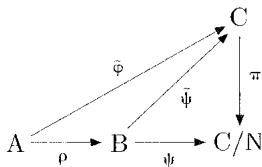
\includegraphics[keepaspectratio]{images/part001_4eedc660.jpg}}

Consider C and C/N as A-algebras by means of \(\tilde{\varphi}\), so that \(\psi\) is a homomorphism of \(A\) -algebras; since B is formally smooth over A, there exists a continuous homomorphism of A-algebras \(\tilde{\psi}: B \to C\) such that \(\pi \circ \tilde{\psi} = \psi\), whence a).

\begin{enumerate}
\def\labelenumi{\alph{enumi})}
\setcounter{enumi}{1}
\item
  It suffices to prove that the product of two formally smooth \(k\)-algebras \(\mathrm{A}_1\) and \(\mathrm{A}_2\) is formally smooth. Let \(\varphi : \mathrm{A}_1 \times \mathrm{A}_2 \to \mathrm{C} / \mathrm{N}\) be a continuous homomorphism of \(k\)-algebras. Set \(e_1 = \varphi(1,0)\), \(e_2 = \varphi(0,1)\), so that \(e_1\) and \(e_2\) are orthogonal idempotents in \(\mathrm{C} / \mathrm{N}\). Let \(\varphi_1 : \mathrm{A}_1 \to (\mathrm{C} / \mathrm{N})e_1\) and \(\varphi_2 : \mathrm{A}_2 \to (\mathrm{C} / \mathrm{N})e_2\) be the maps defined by \(\varphi_1(a_1) = \varphi(a_1,0)\) and \(\varphi_2(a_2) = \varphi(0,a_2)\); these are continuous homomorphisms of \(k\)-algebras, and one has \(\varphi(a_1,a_2) = \varphi_1(a_1) + \varphi_2(a_2)\) for every \((a_1,a_2) \in \mathrm{A}_1 \times \mathrm{A}_2\). There exists an idempotent element \(\tilde{e}_1\) of C such that \(\pi(\tilde{e}_1) = e_1\) (A, VIII, § 9, No. 4, Proposition 7); set \(\tilde{e}_2 = 1 - \tilde{e}_1\), so that \(\pi(\tilde{e}_2) = e_2\). To show that this holds for \(i = 1,2\), the homomorphism \(\mathrm{C}\tilde{e}_i \to (\mathrm{C} / \mathrm{N})e_i\) induced by \(\pi\) is surjective, with kernel \(\mathrm{N}\tilde{e}_i\); since the \(k\)-algebra \(\mathrm{A}_i\) is formally smooth, the homomorphism \(\varphi_i\) admits a continuous lifting \(\tilde{\varphi}_i\) to \(\mathrm{C}\tilde{e}_i\). The map \((a_1,a_2) \mapsto \tilde{\varphi}_1(a_1) + \tilde{\varphi}_2(a_2)\) is a continuous lifting of \(\varphi\) to C.
\item
  Let \(i: \mathrm{A} \to \widehat{\mathrm{A}}\) be the canonical homomorphism. For every ring D equipped with the discrete topology, the map that assigns to a continuous homomorphism \(f: \widehat{\mathrm{A}} \to \mathrm{D}\) the continuous homomorphism \(f \circ i: \mathrm{A} \to \mathrm{D}\) is bijective. Assertion c) follows from this.
\end{enumerate}

The assertion c) of the proposition applies in particular when the topology of \(A\) is the J-adic topology, where \(J\) is a finitely generated ideal: the closure \(\widehat{J}\) of \(J\) in \(\widehat{A}\) is then equal to \(\widehat{JA}\) and the topology of \(\widehat{A}\) is the topology \(\widehat{J}\)-adic (III, § 2, No. 12, Corollary 2 of Proposition 16). Consequently, it is equivalent to say that \(A\) is formally smooth for the J-adic topology or that its separated completion \(\widehat{A}\) is formally smooth for the J-adic topology.

PROPOSITION 4.--- Let k be a ring, A and B k-algebras, J an ideal of A, and K an ideal of B.

\begin{enumerate}
\def\labelenumi{\alph{enumi})}
\item
  Let S be a multiplicative subset of A and T a subset of k whose image in A is contained in S. If \(A\) is formally smooth over \(k\) for the J-adic topology, S \(^{-1}A\) is formally smooth over \(\mathrm{T}^{-1}k\) for the topology \(\mathrm{S}^{-1}\mathrm{J}\)-adic.
\item
  Let \(k'\) be a \(k\)-algebra. If A is formally smooth over \(k\) for the J-adic topology, the \(k'\)-algebra \(A_{(k')}\) is formally smooth over \(k'\) for the \(JA_{(k')}\)-adic topology.
\item
  Let I denote the ideal of A ⊗k B generated by the images of J ⊗k B and A ⊗k K. If A and B are formally smooth over k for the J-adic and K-adic topologies, respectively, then the k-algebra A ⊗k B is formally smooth for the I-adic topology.
\item
  Under the hypotheses of a), let C be a \(\mathrm{T}^{-1}k\)-algebra and N an ideal of square zero in C; endow C and C/N with the discrete topology and denote \(\pi : C \to C/N\) the canonical surjection. Let \(\varphi : S^{-1}A \longrightarrow C/N\) be a homomorphism of \(\mathrm{T}^{-1}k\)-algebras, continuous for the \(\mathrm{S}^{-1}\mathrm{J}\)-adic topology. Denote by i the canonical homomorphism from A into \(S^{-1}A\). The map \(\varphi \circ i\) is a homomorphism of k-algebras, continuous for the J-adic topology, hence admits a lifting \(\tilde{\varphi}_{0} : A \to C\). The elements of \(\tilde{\varphi}_{0}(S)\) are invertible modulo N, hence invertible since N is nilpotent. Consequently there exists a ring homomorphism \(\tilde{\varphi} : S^{-1}A \to C\) such that \(\tilde{\varphi} \circ i = \tilde{\varphi}_{0}\) (II, § 2, No. 1, Proposition 1); by Corollary 3 of Proposition 2 of loc. cit., \(\tilde{\varphi}\) is \(\mathrm{T}^{-1}k\)-linear. We have \(\pi \circ \tilde{\varphi} \circ i = \varphi \circ i\), whence \(\pi \circ \tilde{\varphi} = \varphi\) (loc. cit., Proposition 1), so that \(\tilde{\varphi}\) is a lifting of \(\varphi\).
\item
  Let us place ourselves under the hypotheses of b). Let C be a \(k'\)-algebra and N an ideal of square zero in C; endow C and C/N with the discrete topology. Let \(\varphi : \mathrm{A}_{(k')} \longrightarrow \mathrm{C/N}\) be a homomorphism of \(k'\)-algebras, continuous for the \(J\mathrm{A}_{(k')}\)-adic topology. Let \(i : \mathrm{A} \to \mathrm{A}_{(k')}\) denote the canonical homomorphism. The map \(\varphi \circ i\) is a homomorphism of \(k\)-algebras from A to C/N, continuous for the J-adic topology; if A is formally smooth over \(k\) for the J-adic topology, \(\varphi \circ i\) admits a lifting \(\tilde{\psi} : \mathrm{A} \to \mathrm{C}\). The homomorphism of \(k'\)-algebras \(\tilde{\varphi} : \mathrm{A}_{(k')} \longrightarrow \mathrm{C}\) deduced from \(\tilde{\psi}\) is a lifting of \(\varphi\).
\item
  We place ourselves under the hypotheses of c). The B-algebra A⊗ \(_{k}\) B is formally smooth for the J(A⊗ \(_{k}\) B)-adic topology by b), hence for the I-adic topology; moreover, the canonical homomorphism B → A⊗ \(_{k}\) B is continuous when B is equipped with the K-adic topology and A⊗ \(_{k}\) B with the I-adic topology. Assertion c) therefore follows from Proposition 3, a).
\end{enumerate}

\subsection{Examples of formally smooth algebras}

Let k be a ring.

\begin{enumerate}
\def\labelenumi{\arabic{enumi})}
\tightlist
\item
  Let P be a projective \(k\)-module. The symmetric \(k\)-algebra \(\mathbf{S}_k(\mathrm{P})\) is formally smooth for the discrete topology, and a fortiori for the topology defined by its grading. Indeed, for any \(k\)-algebra C and every ideal N of C, the algebra homomorphisms from \(\mathbf{S}_k(\mathrm{P})\) into C (resp. C/N) are in bijective correspondence with the \(k\)-linear maps from P into C (resp. C/N), and the canonical map \(\mathrm{Hom}_k(\mathrm{P},\mathrm{C}) \to \mathrm{Hom}_k(\mathrm{P},\mathrm{C}/\mathrm{N})\) is surjective.
\end{enumerate}

Therefore (Proposition 3, c)), the \(k\)-algebra \(\widehat{\mathbf{S}}_k(\mathrm{P}) = \prod_{n\geqslant 0}\mathbf{S}_k^n (\mathrm{P})\) is formally smooth (for the product topology of the discrete topologies on the \(\mathbf{S}_k^n (\mathrm{P}))\)); indeed, it is the completion of the \(k\)-algebra \(\mathbf{S}_k(\mathrm{P})\) for the topology defined by the grading.

\begin{enumerate}
\def\labelenumi{\arabic{enumi})}
\setcounter{enumi}{1}
\item
  For any family of indeterminates \(\mathbf{T} = (\mathrm{T}_i)_{i\in I}\), the \(k\)-algebra of polynomials \(k[\mathbf{T}]\) and the \(k\)-algebra of formal power series \(k[[\mathbf{T}]]\), endowed with its canonical topology, are formally smooth; this follows from Example 1. If \(k\) is a field, the purely transcendental extension \(k(\mathbf{T})\) is formally smooth (No. 2, Proposition 4 a)).
\item
  Let \(f \in k[\mathrm{T}]\) be a polynomial in one indeterminate. To say that the \(k\)-algebra \(k[\mathrm{T}]/(f)\) is formally smooth is to say that the following property is satisfied: for every \(k\)-algebra C and every ideal N of square zero in C, every root of \(f\) in C/N lifts to a root of \(f\) in C. This is the case when \(f\) and its derivative \(f'\) generate the unit ideal. Indeed, let \(\alpha\) be a root of \(f\) in C/N and let \(a\) be an element of C lifting \(\alpha\). Then \(f(a)\) belongs to N and consequently \(f'(a)\) is invertible in C; the element \(b = a - f'(a)^{-1}f(a)\) lifts \(\alpha\). Since \(f'(a)^{-1}f(a)\) is of square zero, we have
\end{enumerate}

\[
f (b) = f (a) - f ^ {\prime} (a) f ^ {\prime} (a) ^ {- 1} f (a) = 0.
\]

THEOREM 1 (I. S. Cohen). Let \(k\) be a field and \(K\) a separable extension of \(k\). Then \(K\) is a formally smooth \(k\)-algebra.

Let C be a \(k\)-algebra, N an ideal of square zero in C, \(\pi: \mathrm{C} \to \mathrm{C/N}\) the canonical homomorphism, and \(\varphi: \mathrm{K} \to \mathrm{C/N}\) a homomorphism of \(k\)-algebras. It remains to construct a lifting of \(\varphi\). We distinguish two cases.

\begin{enumerate}
\def\labelenumi{\Alph{enumi})}
\item
  Suppose first that k has characteristic 0. Consider the pairs \((\mathrm{K}^{\prime}, \tilde{\varphi}^{\prime})\), where \(K^{\prime}\) is a subextension of K and \(\tilde{\varphi}^{\prime}: K^{\prime} \to C\) is a lifting of the restriction of \(\varphi\) to \(K^{\prime}\). The set of these pairs, ordered by extension, is inductive; by Zorn's lemma (E, III, p.~20, th. 2), there exists a maximal pair \((\mathrm{K}^{\prime}, \tilde{\varphi}^{\prime})\). Let us prove that \(K^{\prime}\) is equal to K. Let \(x \in K - K^{\prime}\). If x is transcendental over \(K^{\prime}\), the \(K^{\prime}\)-algebra \(\mathrm{K}^{\prime}(x)\) is formally smooth (example 2). If x is algebraic over \(K^{\prime}\), its minimal polynomial \(f \in K^{\prime}[T]\) is relatively prime to its derivative (A, V, p.~37, prop. 4), and \(\mathrm{K}^{\prime}(x)\) identifies with the \(K^{\prime}\)-algebra \(\mathrm{K}^{\prime}[\mathrm{T}]/(f)\), which is therefore a formally smooth \(K^{\prime}\)-algebra (example 3). In both cases, \(\mathrm{K}^{\prime}(x)\) is formally smooth over \(K^{\prime}\), and there exists an extension of \(\tilde{\varphi}^{\prime}\) to \(\mathrm{K}^{\prime}(x)\) that lifts the restriction of \(\varphi\) to \(\mathrm{K}^{\prime}(x)\), contradicting the maximality of \((\mathrm{K}^{\prime}, \tilde{\varphi}^{\prime})\).
\item
  Suppose \(k\) has characteristic \(p \neq 0\). Consider the ring homomorphism F: C → C such that F(x) = x \(^{p}\); one has F(x) = 0 for x ∈ N, so that there exists a unique ring homomorphism λ: C/N → C such that λ ∘ π = F. One has π(λ(π(x))) = π(x \(^{p}\)) = π(x) \(^{p}\); since π is surjective, one therefore has π(λ(z)) = z \(^{p}\) for every element z of C/N. On the other hand, let f: K → K \(^{p}\) be the isomorphism y ↦ y \(^{p}\) and let f \(^{-1}\): K \(^{p}\) → K be the inverse isomorphism. Let g: K \(^{p}\) → C be the composite of the following ring homomorphisms
\end{enumerate}

\[
\mathrm{K} ^ {p} \xrightarrow {f ^ {- 1}} \mathrm{K} \xrightarrow {\varphi} \mathrm{C} / \mathrm{N} \xrightarrow {\lambda} \mathrm{C}.
\]

For every \(x \in K\), one has \(g(x^{p}) = \lambda(\varphi(x))\). Since \(\lambda(\alpha z) = \alpha^{p}\lambda(z)\) for \(\alpha \in k\) and \(z \in C/N\), the map \(g\) is \(k^{p}\)-linear. Since the extension \(K\) of \(k\) is separable, \(k(K^{p})\) is identified with \(k \otimes_{k^{p}} K^{p}\) (A, V, p.~119, remark); consequently there exists a unique homomorphism of \(k\)-algebras \(h: k(K^{p}) \to C\) which coincides with \(g\) on \(K^{p}\).

Let \((a_{i})_{i\in I}\) be a \(p\)-basis of K over \(k(\mathrm{K}^p)\) (A, V, p.~98, theorem 2); for every \(i\in I\), choose an element \(b_{i}\) of C such that \(\pi(b_{i})=\varphi(a_{i})\). One has \(h(a_{i}^{p})=g(a_{i}^{p})=\lambda(\varphi(a_{i}))=\lambda(\pi(b_{i}))=b_{i}^{p}\) for every \(i\in I\). By A, V, p.~94, remark, there exists a homomorphism of \(k\)-algebras \(\tilde{\varphi}:K\to C\), extending \(h\) and such that \(\tilde{\varphi}(a_{i})=b_{i}\) for every \(i\). One has \(\pi(\tilde{\varphi}(a_{i}))=\pi(b_{i})=\varphi(a_{i})\) for every \(i\), and \(\pi(\tilde{\varphi}(x^{p}))=\pi(h(x^{p}))=\pi(g(x^{p}))=\pi(\lambda(\varphi(x)))=\varphi(x^{p})\) for every \(x\in K\). One therefore has \(\pi\circ\tilde{\varphi}=\varphi\), which completes the proof.

COROLLARY.--- Let k be a field, K a separable extension of k, and A a linearly topologized K-algebra. If A is formally smooth over K, it is formally smooth over k.

This follows from the theorem and from prop. 3 a) of no. 2.

Remarks.- 1) Let \(k\) be a field. Every \(k\) -algebra that is étale (A, V, p.~28, def. 1) is formally smooth (loc. cit., p.~34, th. 4, d) and no. 2, prop. 3, b)).

\begin{enumerate}
\def\labelenumi{\arabic{enumi})}
\setcounter{enumi}{1}
\tightlist
\item
  We shall see below (cor. 2 of th. 2 of no. 5) that a field extension which is formally smooth is absolutely regular, hence separable (§ 6, no. 4, example 2).
\end{enumerate}

\subsection{Liftings of homomorphisms in complete filtered algebras}

Let \(k\) be a ring, C a \(k\)-algebra, \((C_n)_{n \in \mathbf{Z}}\) a decreasing filtration of C, compatible with the structure of \(k\)-algebra and such that \(C_0 = C\) (III, § 2, no. 1). Suppose C is separated and complete for the topology defined by this filtration, so that the canonical map \(C \to \varprojlim C / C_n\) is a homeomorphism (loc. cit., no. 6). Let \(m\) be an integer \(>0\). Let us denote \(\pi: C \to C / C_m\) the canonical surjection.

PROPOSITION 5.—Let A be a formally smooth linearly topologized \(k\)-algebra. Every continuous homomorphism of \(k\)-algebras \(\varphi: A \to \mathrm{C/C}_{m}\) admits a continuous lifting to C.

For every integer \(n > m\), let us denote \(\pi_n: \mathrm{C/C}_n \to \mathrm{C/C}_{n-1}\) the canonical surjection. Since C is identified with the projective limit of the \(\mathrm{C/C}_n\), it is equivalent to give a continuous lifting of \(\varphi\) to C or a family \((\varphi_n)_{n > m}\) of continuous homomorphisms of \(k\)-algebras \(\varphi_n: \mathrm{A} \to \mathrm{C/C}_n\), satisfying \(\pi_n \circ \varphi_n = \varphi_{n-1}\). This brings us back, by induction on \(m\), to proving the statement when \(\mathrm{C}_{m+1} = 0\). The ideal \(\mathrm{C}_m\) is then of square zero (since \(2m \geqslant m+1\)), whence the proposition, since A is formally smooth.

Example.—Let C be a \(k\)-algebra and N a nilpotent ideal of C. The proposition applies to the algebra C equipped with the N-adic filtration. If A is a formally smooth linearly topologized \(k\)-algebra, we obtain that every continuous homomorphism from A into the \(k\)-algebra C/N, endowed with the discrete topology, lifts to a continuous homomorphism from A into the \(k\)-algebra C, equipped with the discrete topology.

\subsection{Formally smooth quotients of algebras}

THEOREM 2.--- Let k be a ring, A a k-algebra, and J an ideal of A such that the k-algebra A/J is formally smooth. Endow A with the J-adic topology. The following conditions are equivalent:

\begin{enumerate}
\def\labelenumi{(\roman{enumi})}
\item
  the topological k-algebra A is formally smooth;
\item
  the \(A/\mathrm{J}\)-module \(\mathrm{J}/\mathrm{J}^2\) is projective and the canonical homomorphism (§ 5, no. 2)
\end{enumerate}

\[
\beta : \mathbf {S} _ {\mathrm{A/J}} (\mathrm{J} / \mathrm{J} ^ {2}) \rightarrow \operatorname{gr} _ {\mathrm{J}} (\mathrm{A})
\]

is bijective;

\begin{enumerate}
\def\labelenumi{(\roman{enumi})}
\setcounter{enumi}{2}
\tightlist
\item
  the A/J-module J/J \(^{2}\) is projective and there exists an isomorphism of topological k-algebras from the separated completion of A onto the completion of the graded algebra \(\mathsf{S}_{A/J}\) (J/J \(^{2}\)).
\end{enumerate}

If A is Noetherian, these conditions are also equivalent to:

\begin{enumerate}
\def\labelenumi{(\roman{enumi})}
\setcounter{enumi}{3}
\tightlist
\item
  the ideal J is completely secant.
\end{enumerate}

First observe that (iii) implies (i): indeed, under the hypotheses of (iii), the algebra \(\mathsf{S}_{\mathrm{A}/\mathrm{J}}(\mathrm{J}/\mathrm{J}^{2})\) , endowed with the topology associated with its grading, is formally smooth over A/J (no. 3, example 1), hence over k (no. 2, prop. 3, a)); assertion (i) then follows from prop. 3, c) of no. 2.

Let \(\widehat{\mathbf{A}}\) be the separated completion of the algebra A and \(\widehat{\mathbf{J}}\) the separated completion of J. The canonical homomorphism \(i: \mathbf{A} \to \widehat{\mathbf{A}}\) induces an isomorphism \(\mathrm{A} / \mathrm{J} \longrightarrow \widehat{\mathrm{A}} / \widehat{\mathrm{J}}\) (III, § 2, no. 12, formula (21)). Let \(\varphi: \mathrm{A} / \mathrm{J} \to \widehat{\mathrm{A}}\) be a lifting of this isomorphism (no. 4, prop. 5). Denote \(\lambda: \widehat{\mathrm{J}} \to \mathrm{J} / \mathrm{J}^2\) the surjection deduced from the canonical isomorphism \(\mathrm{J} / \mathrm{J}^2 \longrightarrow \widehat{\mathrm{J}} / \widehat{\mathrm{J}}^2\) (III, § 2, no. 12, formula (21)). Let \(a\) be an element of A, \(\bar{a}\) its class in \(\mathrm{A} / \mathrm{J}\), and let \(z\) be an element of \(\widehat{\mathrm{J}}\); one has \(\varphi(\bar{a}) \equiv i(a)\) (mod. \(\widehat{\mathrm{J}}\)), whence \(\varphi(\bar{a})z \equiv i(a)z\) (mod. \(\widehat{\mathrm{J}}^2\)) and \(\lambda(\varphi(\bar{a})z) = \lambda(i(a)z) = \bar{a}\lambda(z)\). In other words, \(\lambda\) is A/J-linear when one equips \(\widehat{\mathbf{J}}\) with the structure of an A/J-module induced by \(\varphi\).

Suppose that the homomorphism \(\lambda\) admits an A/J-linear section \(\sigma : J/J^{2} \longrightarrow \widehat{J}\). Let \(S\) be the \(k\)-graded algebra \(S_{A/J}(J/J^{2})\) and \(\widehat{S}\) its completion. Let

\[
\theta : \mathsf {S} \to \widehat {\mathsf {A}}
\]

the homomorphism of \(k\)-algebras such that \(\theta(x) = \varphi(x)\) for \(x\) in \(\mathbf{S}^0 = \mathrm{A}/\mathrm{J}\), and \(\theta(x) = \sigma(x)\) for \(x\) in \(\mathbf{S}^1 = \mathrm{J}/\mathrm{J}^2\). Since \(\theta\) maps \(\mathbf{S}^1\) into \(\widehat{\mathbf{J}}\), it maps \(\mathbf{S}^n\) into \(\widehat{\mathbf{J}}^n\) and therefore extends to a continuous homomorphism \(\widehat{\boldsymbol{\theta}}: \widehat{\mathbf{S}} \to \widehat{\mathbf{A}}\). The map \(\mathrm{gr}_1(\boldsymbol{\theta}): \mathrm{J}/\mathrm{J}^2 \longrightarrow \widehat{\mathrm{J}}/\widehat{\mathrm{J}}^2\) is the composite of \(\sigma\) with the canonical surjection \(\widehat{\mathrm{J}} \longrightarrow \widehat{\mathrm{J}}/\widehat{\mathrm{J}}^2\); since \(\sigma\) is a section of \(\lambda\), \(\mathrm{gr}_1(\boldsymbol{\theta})\) coincides with the canonical isomorphism from \(\mathrm{J}/\mathrm{J}^2\) onto \(\widehat{\mathrm{J}}/\widehat{\mathrm{J}}^2\). Consequently \(\mathrm{gr}(\boldsymbol{\theta}): \mathbf{S} \to \mathrm{gr}_{\widehat{\mathbf{J}}}(\widehat{\mathbf{A}})\) is the composite of the canonical surjection \(\beta\) with the canonical isomorphism \(\mathrm{gr}_\mathrm{J}(\mathrm{A}) \to \mathrm{gr}_{\widehat{\mathbf{J}}}(\widehat{\mathbf{A}})\) (III, § 2, no. 12, formula (22)).

Now let us prove the implication (ii)⇒(iii). Under hypothesis (ii), the A/J-module J/J² is projective, so λ admits an A/J-linear section; the homomorphism \(\widehat{\boldsymbol{\theta}}:\widehat{\mathbf{S}}\to\widehat{\mathbf{A}}\) associated with this section by the preceding construction induces, by hypothesis, an isomorphism on the associated graded modules, hence is bijective (III, § 2, no. 8, cor. 3 of th. 1), which proves (iii).

Let us prove (i)⇒(ii). Suppose the topological k-algebra A is formally smooth. First we prove that the A/J-module \(J/J^{2}\) is projective. Let M be an \(A/J\)-module and \(f:M\to J/J^{2}\) a surjective A/J-linear map; the goal is to prove that f admits an A/J-linear section.

Let \(\pi: A/J^{2} \to A/J\) be the canonical surjection. By Remark 1 of No. 2, there exists an isomorphism of \(k\)-algebras \(\psi: A/J \oplus J/J^{2} \longrightarrow A/J^{2}\) such that \(\pi(\psi(y,z)) = y\) and \(\psi(0,z) = z\) for \(y \in A/J\), \(z \in J/J^{2}\). Consider the \(k\)-algebra (A/J) \(\oplus M\) (No. 1, example) and the map \(u: (A/J) \oplus M \to A/J^{2}\) such that \(u(x,m) = \psi(x,f(m))\). This is a surjective homomorphism of \(k\)-algebras, whose kernel is the kernel of \(f\) in M, hence is nilpotent of square zero. The canonical surjection \(\rho: A \to A/J^{2}\) is continuous; since A is formally smooth as a topological \(k\)-algebra, there exists a homomorphism of \(k\)-algebras \(\tilde{\rho}: A \to (A/J) \oplus M\) such that \(u \circ \tilde{\rho} = \rho\). Since \(\mathrm{pr}_{1} = \pi \circ \psi = \pi \circ u\), one has \(\mathrm{pr}_{1} \circ \tilde{\rho} = \pi \circ u \circ \tilde{\rho} = \pi \circ \rho\), so that \(\mathrm{pr}_{1} \circ \tilde{\rho}\) is the canonical surjection of A onto A/J. We therefore have \(\tilde{\rho}(J) \subset M\) and consequently \(\tilde{\rho}(J^{2}) = 0\), so that \(\tilde{\rho}\) induces an A/J-linear map \(s: J/J^{2} \to M\). One has \(u \circ \tilde{\rho} = \rho\) and \(\mathrm{pr}_{2} \circ \psi^{-1} \circ u(y,m) = f(m)\) for \(y \in A/J\) and \(m \in M\). Let \(x \in J\), and let \(\bar{x}\) be its class in \(J/J^{2}\); one has \(f(s(\bar{x})) = f(\mathrm{pr}_{2}(\tilde{\rho}(x))) = \mathrm{pr}_{2}(\psi^{-1}(\bar{x})) = \bar{x}\). Thus \(s\) is a section of \(f\).

It remains to prove that the homomorphism \(\beta\) is injective. Since the A/J-module \(J/J^{2}\) is projective, \(\lambda\) admits an A/J-linear section; denote by \(\theta: S \to \widehat{A}\) the associated homomorphism. The homomorphism gr(θ) is identified with \(\beta\). Let \(m\) be an integer; denote by \(\Sigma_{m}\) the graded \(k\)-algebra quotient of \(S\) by the ideal \(\sum_{i > m} S^{i}\) and \(\theta_{m}: \Sigma_{m} \to A/J^{m+1}\) the homomorphism deduced from \(\theta\). The composite of \(\theta_{m}\) with the canonical surjection \(A/J^{m+1} \longrightarrow A/J\) is the canonical projection of \(\Sigma_{m}\) onto \(S^{0} = A/J\); consequently the kernel of \(\theta_{m}\) is a nilpotent ideal. By the example in no. 4, there exists a lifting \(\psi_{m}: A \to \Sigma_{m}\) of the canonical surjection \(A \to A/J^{m+1}\). Since the composite of \(\psi_{m}\) with the canonical projection from \(\Sigma_{m}\) onto A/J is the canonical surjection, \(\psi_{m}(J)\) consists of elements of degree \(>0\). By passing to the associated graded objects, we deduce from \(\psi_{m}\) a \(k\)-linear graded map gr(\(\psi_{m}\)): gr \(_{J}(A) \to \Sigma_{m}\) such that gr \(_{m}(\theta) \circ\) gr \(_{m}(\psi_{m}) = \text{Id}_{J^{m}/J^{m+1}}\). It follows that gr \(_{m}(\theta)\), hence also \(\beta_{m}\), is injective, which completes the proof of (ii).

Finally, when A is Noetherian, conditions (ii) and (iv) are equivalent (§ 5, no. 2, th. 1).

COROLLARY 1.--- Let \(k\) a field and A a \(k\) -local Noetherian algebra such that the extension \(\kappa_{A}\) of \(k\) Let it be separable. The following conditions are equivalent:

\begin{enumerate}
\def\labelenumi{(\roman{enumi})}
\item
  the \(k\) -algebra A is formally smooth for the topology \(\mathfrak{m}_{\mathrm{A}}\) -adic;
\item
  the ring A is regular;
\item
  the \(k\)-algebra A is absolutely regular (\(\S 6, \mathrm{n}^{\circ} 4\), def. 1);
\item
  the k-algebra \(\hat{A}\) is isomorphic to \(\kappa_{A}[[T_{1},\ldots,T_{n}]]\) , with \(n=\dim A\) .
\end{enumerate}

Conditions (ii) and (iii) are equivalent by Example 3 of § 6, No. 4, and amount to saying that the ideal \(\mathfrak{m}_{\mathrm{A}}\) is completely secant (VIII, § 5, no. 2, th. 1). Moreover, every ring isomorphism of \(\widehat{\mathrm{A}}\) on \(\kappa_{\mathrm{A}}[[\mathrm{T}_{1},\ldots,\mathrm{T}_{n}]]\) is bicontinuous, since these are local rings. Since the \(k\) -algebra \(\mathrm{A}/\mathfrak{m}_{\mathrm{A}}\) is formally smooth (no. 3, th. 1), the corollary follows from th. 2 applied with \(\mathrm{J}=\mathfrak{m}_{\mathrm{A}}\) .

COROLLARY 2.--- Let k be a field, A a Noetherian k-algebra, and J an ideal of A contained in the radical of A. Suppose the k-algebra A is formally smooth for the J-adic topology. Then it is absolutely regular.

Indeed, let \(k'\) be a finite extension of \(k\) and \(A'\) the A-algebra \(A_{(k')}\); it remains to prove that, for every maximal ideal \(\mathfrak{m}'\) of \(A'\), the Noetherian local ring \(A_{\mathfrak{m}'}'\) is regular. Now we have \(JA' \subset \mathfrak{m}'\): indeed, the inverse image of \(\mathfrak{m}'\) in A is a maximal ideal of A (V, § 2, no. 1, prop. 1), hence contains J. The \(k'\)-algebra \(A'\) is formally smooth for the \(JA'\)-adic topology (no. 2, prop. 4, b)), and the \(k'\)-algebra \(A_{\mathfrak{m}'}'\) is formally smooth for the \(JA_{\mathfrak{m}'}'\)-adic topology (no. 2, prop. 4, a)), hence also for the \(\mathfrak{m}'A_{\mathfrak{m}'}'\)-adic topology. Let \(k_0\) be the prime subfield of \(k'\). Then \(A_{\mathfrak{m}'}'\) is formally smooth over \(k_0\) for the \(\mathfrak{m}'A_{\mathfrak{m}'}'\)-adic topology (cor. of th. 1 of no. 3); since \(\kappa(\mathfrak{m}')\) is separable over \(k_0\), the ring \(A_{\mathfrak{m}'}'\) is regular (cor. 1).

COROLLARY 3.--- Let k be a ring and A a formally smooth k-algebra.

\begin{enumerate}
\def\labelenumi{\alph{enumi})}
\item
  The A-module \(\Omega_k(A)\) is projective.
\item
  Suppose that the ring A ⊗k A is Noetherian. Let μ : A ⊗k A → A be the homomorphism such that μ(x ⊗ y) = xy; then the ideal Ker(μ) is completely secant.
\end{enumerate}

The \(k\)-algebras A and \(\mathbf{A} \otimes_{k} \mathbf{A}\) are formally smooth (no. 2, prop. 4, c)), and A is isomorphic to the quotient of \(\mathbf{A} \otimes_{k} \mathbf{A}\) by the kernel I of \(\mu\). By definition, \(\Omega_{k}(\mathbf{A}) = \mathbf{I}/\mathbf{I}^{2}\). Thus a) and b) follow from th. 2.

\subsection{Extension of the base field in regular algebras (nonzero characteristic)}

Let \(k\) be a ring and \(\rho: A \to B\) a homomorphism of \(k\)-algebras. The homomorphism \(\rho\) induces an A-linear map \(\Omega(\rho): \Omega_k(A) \to \Omega_k(B)\), and consequently a B-linear map \(\Omega_0(\rho): B \otimes_A \Omega_k(A) \to \Omega_k(B)\) (A, III, p.~135). Let \(\mathbf{T} = (\mathrm{T}_i)_{i \in I}\) be a family of indeterminates, and \(\mathbf{t} = (t_i)_{i \in I}\) a family of elements of B; for every polynomial \(f = \sum_{\alpha \in \mathbf{N}^{(I)}} c_\alpha \mathbf{T}^\alpha\) of A{[} \(\mathbf{T}\) {]}, let us denote by \(d^{A} f(\mathbf{t})\) the element \(\sum_{\alpha} \mathbf{t}^\alpha \otimes dc_\alpha\) of \(B \otimes_A \Omega_k(A)\).

Lemma 1.—Suppose that the A-algebra B admits a generating family \(\mathbf{t} = (t_i)_{i\in I}\), subject to the relations \(f_\lambda \in \mathrm{A}[\mathbf{T}]\) (\(\lambda \in \Lambda\)). The B-linear homomorphism

\[
\psi : (\mathrm{B} \otimes_ {\mathrm{A}} \Omega_ {k} (\mathrm{A})) \oplus \mathrm{B} ^ {(\mathrm{I})} \longrightarrow \Omega_ {k} (\mathrm{B})
\]

defined by \(\psi(\alpha,(b_i)) = \Omega_0(\rho)(\alpha) + \sum_{i\in I}b_i\,dt_i\) is surjective; its kernel is generated by the elements \(n_{\lambda} = \left(d^{A}f_{\lambda}(\mathbf{t}),\left(\frac{\partial f_{\lambda}}{\partial\mathrm{T}_{i}}(\mathbf{t})\right)_{i\in I}\right)\) for \(\lambda \in \Lambda\).

Consider the sequence of B-modules and B-linear maps

\[
\mathrm{B} ^ {(\Lambda)} \xrightarrow {\varphi} (\mathrm{B} \otimes_ {\mathrm{A}} \Omega_ {k} (\mathrm{A})) \oplus \mathrm{B} ^ {(\mathrm{I})} \xrightarrow {\psi} \Omega_ {k} (\mathrm{B}) \longrightarrow 0,
\]

where \(\varphi\) is the homomorphism such that \(\varphi(e_{\lambda}) = n_{\lambda}\) ; it remains to show that this sequence is exact. By A, II, p.~36, th. 1, it suffices to prove that, for every B-module M, the sequence

\[
0 \to \operatorname{Hom} _ {\mathrm{B}} (\Omega _{k}(\mathrm{B}), \mathrm{M}) \xrightarrow {\operatorname{Hom}(\psi,1)} \operatorname{Hom} _{\mathrm{B}} ((\mathrm{B} \otimes_{\mathrm{A}} \Omega _{k}(\mathrm{A})) \oplus \mathrm{B}^{(\mathrm{I})}, \mathrm{M}) \xrightarrow {\operatorname{Hom}(\varphi,1)} \operatorname{Hom}_{\mathrm{B}}(\mathrm{B}^{(\Lambda)}, \mathrm{M})
\]

is exact. Given the universal property of the module of differentials (A, III, p.~134), this sequence identifies with

\[
0 \to \mathrm{D} _ {k} (\mathrm{B}, \mathrm{M}) \xrightarrow {\psi^ {\prime}} \mathrm{D} _ {k} (\mathrm{A}, \mathrm{M}) \oplus \mathrm{M} ^ {\mathrm{I}} \xrightarrow {\varphi^ {\prime}} \mathrm{M} ^ {\Lambda}
\]

where \(\psi^{\prime}(\mathrm{D}) = (\mathrm{D}\circ \rho,(\mathrm{D}(t_{i}))_{i\in I})\) and \(\varphi^{\prime}(\Delta,(m_{i})) = \big(f_{\lambda}^{\Delta}(\mathbf{t}) + \sum_{i}\frac{\partial f_{\lambda}}{\partial\mathrm{T}_{i}}(\mathbf{t})m_{i}\big)_{\lambda \in \Lambda}\) (in accordance with A, V, p.~121, for every polynomial \(f = \sum_{\alpha \in \mathbf{N}^{(I)}}c_{\alpha}\mathbf{T}^{\alpha}\) of A{[}T{]}, we denote \(f^{\Delta}(\mathbf{t})\) as the element \(\sum_{\alpha}\mathbf{t}^{\alpha}\Delta(c_{\alpha})\). Now the exactness of this sequence follows from loc. cit., prop. 1, taking into account that a derivation D : B → M is \(k\)-linear if and only if \(D\circ\rho\) is so.

Let A be a ring. There exists a unique structure of \(\mathbf{Z}\)-algebra on A; we simply denote \(\Omega(A)\) the A-module \(\Omega_{\mathbf{Z}}(\mathrm{A})\). If \(\rho : k \to \mathrm{A}\) is a ring homomorphism, we have a canonical exact sequence of A-modules (A, III, p.~136, prop. 21) \(\mathrm{A} \otimes_k \Omega(k) \to \Omega(\mathrm{A}) \to \Omega_k(\mathrm{A}) \to 0\).

Suppose that A contains a subfield, and let P be the prime subfield of A; then \(\Omega(\mathrm{P})\) is zero and the canonical homomorphism of A-modules \(\Omega(\mathrm{A}) \to \Omega_{\mathrm{P}}(\mathrm{A})\) is bijective. If moreover A has characteristic \(p \neq 0\) (which means by definition that \(p\) is a prime number, \(p1_{\mathrm{A}} = 0\), and \(1_{\mathrm{A}} \neq 0\)), then P is identified with \(\mathbf{F}_p\). Moreover, every derivation of A vanishes on the subring \(\mathbf{A}^p\); for every subring \(k\) of A contained in \(\mathbf{A}^p\) (and, in particular, for every perfect subfield \(k\) of A), the canonical map \(\Omega(\mathrm{A}) \to \Omega_k(\mathrm{A})\) is bijective.

Let A be a ring of characteristic \(p \neq 0\) and \((f_i)_{1 \leqslant i \leqslant n}\) a finite sequence of elements of A. Denote by \(A_n\) the quotient ring of the polynomial ring \(A[T_1, \ldots, T_n]\) by the ideal generated by the polynomials \(T_i^p - f_i\) , for \(1 \leqslant i \leqslant n\) .

Lemma 2.—Suppose the ring A is local and Noetherian. Then \(A_{n}\) is local and Noetherian. The following conditions are equivalent:

\begin{enumerate}
\def\labelenumi{(\roman{enumi})}
\item
  \(A_{n}\) is regular;
\item
  A is regular and the elements \(1 \otimes df_{i}\) of the \(\kappa_{A}\) -vector space \(\kappa_{A} \otimes_{A} \Omega(A)\) are linearly independent.
\end{enumerate}

The ring \(A_{n}\) is Noetherian (III, § 2, cor. 3 of th. 2). The A-module \(A_{n}\) is free, hence faithfully flat; if \(A_{n}\) is regular, then A is regular (§ 4, no. 5, prop. 8 b)). We shall reason by induction on n, the lemma being evident if n = 0.

\begin{enumerate}
\def\labelenumi{\Alph{enumi})}
\tightlist
\item
  Let us first treat the case n = 1, setting \(T_{1} = T\), \(f_{1} = f\). Let a denote the class of f in \(\kappa_{A}\) and distinguish two cases, according as a belongs or does not belong to \(\kappa_{A}^{p}\). If \(a \notin \kappa_{A}^{p}\), then the polynomial \(T^{p} - a\) is irreducible in \(\kappa_{A}\) (A, V, p.~24, lemma 1) and \(\kappa_{A} \otimes_{A} A_{1}\) is isomorphic to the field \(\kappa_{A}[T]/(T^{p} - a)\). The ideal \(m_{A}A_{1}\) of \(A_{1}\) is therefore maximal, so that the ring \(A_{1}\) is local (V, § 2, no. 1, prop. 1). If A is regular, \(A_{1}\) is regular (VIII, § 5, no. 1, prop. 1). According to A, V, p.~99, prop. 6, the element da of \(\Omega(\kappa_{A})\) is not zero; since it is the image under the canonical map \(\kappa_{A} \otimes_{A} \Omega(A) \to \Omega(\kappa_{A})\) of \(1 \otimes df\), the latter is not zero. This proves the lemma in this case.
\end{enumerate}

Now suppose that \(a\) belongs to \(\kappa_{\mathrm{A}}^{p}\). There therefore exists an element \(g\) of A such that \(f - g^{p} \in \mathfrak{m}_{\mathrm{A}}\). Set \(h = f - g^{p}\). Since \(\mathrm{T}^{p} - f = (\mathrm{T} - g)^{p} - h\), the A-algebra \(A_{1}\) is isomorphic to \(\mathrm{A}[\mathrm{T}] / (\mathrm{T}^{p} - h)\). According to VIII, § 5, no. 4, prop. 4, the ring \(A_{1}\) is local and, for it to be regular, it is necessary and sufficient that A be regular and that \(h\) not belong to \(\mathfrak{m}_{\mathrm{A}}^{2}\). Now, since \(\kappa_{A}\) is formally smooth over the prime field (no. 3, th. 1), the canonical map

\[
\bar {d}: \mathfrak {m} _ {\mathrm{A}} / \mathfrak {m} _ {\mathrm{A}} ^ {2} \to \kappa_ {\mathrm{A}} \otimes_ {\mathrm{A}} \Omega (\mathrm{A})
\]

is injective (no. 2, remark 1); but the image under \(\bar{d}\) of the class of \(h\) modulo \(\mathfrak{m}_{\mathrm{A}}^{2}\) is equal to \(1 \otimes dh = 1 \otimes d(f - g^{p}) = 1 \otimes df\). This proves the lemma in this second case and completes the proof of the case \(n = 1\).

\begin{enumerate}
\def\labelenumi{\Alph{enumi})}
\setcounter{enumi}{1}
\tightlist
\item
  Suppose \(n > 1\) . The ring \(\mathrm{A}_{1}\) is local and Noetherian by the case already treated. The \(\mathrm{A}_{1}\) -algebra \(\mathrm{A}_{n}\) is identified with the quotient of \(\mathrm{A}_{1}[\mathrm{T}_{2},\ldots ,\mathrm{T}_{n}]\) by the ideal generated by the \(\mathrm{T}_i^p -f_i\) , \(i\geqslant 2\) ; by the induction hypothesis, it is a local ring and condition (i) is equivalent to the conjunction of the following two conditions:
\end{enumerate}

(i') A \(_{1}\) is regular;

(i'\,') the elements \(1 \otimes df_2, \ldots, 1 \otimes df_n\) of the \(\kappa_{\mathrm{A}_1}\) -vector space \(\kappa_{\mathrm{A}_1} \otimes_{\mathrm{A}_1} \Omega(\mathrm{A}_1)\) are linearly independent.

But (i') is equivalent, as we have just seen, to

(ii') A is regular and the element \(1 \otimes df_{1}\) of the \(\kappa_{A}\)-vector space \(\kappa_{A} \otimes_{A} \Omega(A)\) is not zero.

By Lemma 1, the canonical homomorphism \(\mathrm{A}_{1} \otimes_{\mathrm{A}} \Omega(\mathrm{A}) \to \Omega(\mathrm{A}_{1})\) induces an isomorphism of \(((\mathrm{A}_{1} \otimes_{\mathrm{A}} \Omega(\mathrm{A})) / \mathrm{A}_{1}(1 \otimes df_{1})) \oplus \mathrm{A}_{1}\) onto \(\Omega(\mathrm{A}_{1})\), and consequently an injective homomorphism of \((\kappa_{\mathrm{A}_{1}} \otimes_{\mathrm{A}} \Omega(\mathrm{A})) / \kappa_{\mathrm{A}_{1}}(1 \otimes df_{1})\) into \(\kappa_{\mathrm{A}_{1}} \otimes_{\mathrm{A}_{1}} \Omega(\mathrm{A}_{1})\). Since \(\kappa_{\mathrm{A}_{1}} \otimes_{\mathrm{A}} \Omega(\mathrm{A})\) is identified with \(\kappa_{\mathrm{A}_{1}} \otimes_{\kappa_{\mathrm{A}}} (\kappa_{\mathrm{A}} \otimes_{\mathrm{A}} \Omega(\mathrm{A}))\), assertion (i'') is therefore equivalent to:

(ii'') the elements \(1 \otimes df_2, \ldots, 1 \otimes df_n\) are linearly independent in \((\kappa_{\mathrm{A}} \otimes_{\mathrm{A}} \Omega(\mathrm{A})) / \kappa_{\mathrm{A}}(1 \otimes df_1)\).

But the conjunction of (ii') and (ii'') is equivalent to (ii), which proves the lemma.

PROPOSITION 6. Let \(k\) be a field of characteristic \(p \neq 0\), \(k'\) be a radical extension of \(k\), of finite degree and height \(\leqslant 1\), and let A be a local regular \(k\)-algebra. Then \(\mathrm{A}_{(k')}\) is a local ring and the following conditions are equivalent:

\begin{enumerate}
\def\labelenumi{(\roman{enumi})}
\item
  the ring \(A_{(k')}\) is regular;
\item
  the \(\kappa_{A}\)-linear map
\end{enumerate}

\[
\kappa_ {\mathrm{A}} \otimes_ {k ^ {\prime p}} \Omega_ {k ^ {p}} (k ^ {\prime p}) \longrightarrow \kappa_ {\mathrm{A}} \otimes_ {\mathrm{A}} \Omega (\mathrm{A})
\]

deduced from the canonical injection \(k^{\prime p}\to \mathrm{A}\) is injective.

Indeed, let \((x_{i})_{i\in \mathrm{I}}\) be a finite \(p\)-basis of \(k'\) over \(k\) (A, V, p.~98); for all \(i\in \mathrm{I}\), set \(f_{i} = x_{i}^{p}\in k\). The \(k\)-algebra \(k'\) is identified with the quotient of \(k[(\mathrm{T}_i)_{i\in \mathrm{I}}]\) by the ideal generated by the polynomials \(\mathrm{T}_i^p - f_i\), hence the A-algebra \(\mathrm{A}_{(k')}\) is the quotient of \(\mathrm{A}[(\mathrm{T}_i)_{i\in \mathrm{I}}]\) by the ideal generated by the polynomials \(\mathrm{T}_i^p - f_i1_{\mathrm{A}}\).

Moreover, \((f_{i})_{i\in\mathrm{I}}\) is a p-basis of \(k^{\prime p}\) over \(k^{p}\), and the \(k^{\prime p}\)-vector space \(\Omega_{k^{p}}(k^{\prime p})\) has the family of \(df_{i}\) as a basis (A, V, p.~97, th. 1). Proposition 6 then follows from Lemma 2.

\subsection{A criterion for formally smooth local algebras}

PROPOSITION 7. Let \(k_{0}\) be a ring, \(k\) a \(k_{0}\)-algebra, A a \(k\)-algebra, and \(\mathfrak{m}\) a maximal ideal of A. We assume that \(k\) and A/\(\mathfrak{m}\) are formally smooth over \(k_{0}\). For A to be formally smooth over \(k\) for the \(\mathfrak{m}\)-adic topology, it is necessary and sufficient that the following two conditions be satisfied:

\begin{enumerate}
\def\labelenumi{(\roman{enumi})}
\item
  the canonical homomorphism \(\mathsf{S}_{\mathrm{A} / \mathfrak{m}}(\mathfrak{m} / \mathfrak{m}^{2})\to \mathrm{gr}_{\mathfrak{m}}(\mathrm{A})\) is bijective;
\item
  the A/m-linear map
\end{enumerate}

\[
\omega : \mathrm{A} / \mathfrak {m} \otimes_ {k} \Omega_ {k _ {0}} (k) \longrightarrow \mathrm{A} / \mathfrak {m} \otimes_ {\mathrm{A}} \Omega_ {k _ {0}} (\mathrm{A})
\]

deduced from the canonical map \(k \to A\) is injective.

Let \(d_{k}:k\to \Omega_{k_{0}}(k)\) and \(d_{\mathrm{A}}:\mathrm{A}\to \Omega_{k_0}(\mathrm{A})\) be the universal \(k_{0}\)-derivations.

Suppose first that A is formally smooth over \(k\) for the \(\mathfrak{m}\)-adic topology. Then A is formally smooth over \(k_{0}\) for the \(\mathfrak{m}\)-adic topology (\(n^{\circ} 2\), prop. 3, a)), which is equivalent to (i) (\(n^{\circ} 5\), th. 2). Moreover, the \(k_{0}\)-derivation \(\lambda \mapsto 1 \otimes d_{k}(\lambda)\) of \(k\) in \(A/\mathfrak{m} \otimes_{k} \Omega_{k_{0}}(k)\) can be extended to a \(k_{0}\)-derivation of A into \(A/\mathfrak{m} \otimes_{k} \Omega_{k_{0}}(k)\) (\(n^{\circ} 2\), remark 2). There therefore exists an A-linear map \(u: \Omega_{k_{0}}(A) \to A/\mathfrak{m} \otimes_{k} \Omega_{k_{0}}(k)\) such that \(u(d_{A}(\lambda 1_{A})) = 1 \otimes d_{k}(\lambda)\) for every \(\lambda \in k\). The \(A/\mathfrak{m}\)-linear map \(A/\mathfrak{m} \otimes_{A} \Omega_{k_{0}}(A) \longrightarrow A/\mathfrak{m} \otimes_{k} \Omega_{k_{0}}(k)\) deduced from \(u\) is a retraction of \(\omega\), which proves (ii).

Conversely, suppose conditions (i) and (ii) are satisfied. Then A is formally smooth over \(k_{0}\) for the \(\mathfrak{m}\)-adic topology (\(n^{\circ}5\), th. 2) and the A-module \(\Omega_{k_{0}}(A)\) is projective (\(n^{\circ}5\), cor. 3 of th. 2). Fix an integer \(r \geqslant 0\) and consider the map, linear over \(A/\mathfrak{m}^{r}\),

\[
\omega_ {r}: \mathrm{A} / \mathfrak {m} ^ {r} \otimes_ {k} \Omega_ {k _ {0}} (k) \longrightarrow \mathrm{A} / \mathfrak {m} ^ {r} \otimes_ {\mathrm{A}} \Omega_ {k _ {0}} (\mathrm{A})
\]

deduced from the canonical map \(k\to\mathrm{A}\). Let \((\lambda_{i})_{i\in\mathrm{I}}\) be a family of elements of \(k\) such that the \(d_{k}(\lambda_{i})\) form a basis of the \(k\)-vector space \(\Omega_{k_{0}}(k)\). By (ii), the elements \(1 \otimes d_{A}(\lambda_{i}1_{A})\) are linearly independent in A/m \(\otimes_{\mathrm{A}} \Omega_{k_0}(\mathrm{A})\). By II, § 3, no. 2, cor. 1 and 2 of prop. 5, the \(1 \otimes d_{A}(\lambda_{i}1_{A})\) form a basis of a direct summand of the A/m \(^{r}\)-module A/m \(^{r} \otimes_{\mathrm{A}} \Omega_{k_0}(\mathrm{A})\). There therefore exists a map, linear over A/m \(^{r}\),

\[
u _ {r}: \mathrm{A} / \mathfrak {m} ^ {r} \otimes_ {\mathrm{A}} \Omega_ {k _ {0}} (\mathrm{A}) \longrightarrow \mathrm{A} / \mathfrak {m} ^ {r} \otimes_ {k} \Omega_ {k _ {0}} (k)
\]

such that \(u_r(1 \otimes d_A(\lambda_i 1_A)) = 1 \otimes d_k(\lambda_i)\) for every \(i\) , hence \(u_r \circ \omega_r = \mathrm{Id}\) .

Let us now verify that A is formally smooth over \(k\) for the m-adic topology. Let C be a \(k\)-algebra, N an ideal of square zero in C, and \(\pi: C \to C/N\) the canonical surjection; endow C and C/N with the discrete topology. Let \(\varphi: A \to C/N\) be a continuous homomorphism of \(k\)-algebras. Since A is formally smooth over \(k_0\) for the m-adic topology, there exists a continuous homomorphism of \(k_0\)-algebras \(\tilde{\varphi}_0: A \to C\) such that \(\pi \circ \tilde{\varphi}_0 = \varphi\). According to Proposition 1 of No. 1, the homomorphisms of \(k_0\)-algebras \(\tilde{\varphi}: A \to C\) such that \(\pi \circ \tilde{\varphi} = \varphi\) are the maps \(x \mapsto v(d_A(x)) + \tilde{\varphi}_0(x)\), where \(v\) ranges over \(\mathrm{Hom}_{A}(\Omega_{k_0}(A), N)\). It remains to choose \(v\) so that \(\tilde{\varphi}\) is a homomorphism of \(k\)-algebras. The map \(\lambda \mapsto \lambda 1_C - \tilde{\varphi}_0(\lambda 1_A)\) is a \(k_0\)-derivation from \(k\) into N (loc. cit.), hence can be written \(h \circ d_k\) with \(h \in \mathrm{Hom}_k(\Omega_{k_0}(k), N)\).

Let us choose an integer \(r\) such that the kernel of \(\varphi\) contains \(\mathfrak{m}^r\). The A-module N is annihilated by \(\mathfrak{m}^r\), and it suffices to take for \(v\) the composite of the sequence of homomorphisms

\[
\Omega_ {k _ {0}} (\mathrm{A}) \longrightarrow \mathrm{A} / \mathfrak {m} ^ {r} \otimes_ {\mathrm{A}} \Omega_ {k _ {0}} (\mathrm{A}) \xrightarrow {u _ {r}} \mathrm{A} / \mathfrak {m} ^ {r} \otimes_ {k} \Omega_ {k _ {0}} (k) \xrightarrow {h ^ {\prime}} \mathrm{N},
\]

where \(h'\) is deduced from \(h\). Indeed, we have, for \(\lambda \in k\):

\[
v \left(d _ {\mathrm{A}} \left(\lambda 1 _ {\mathrm{A}}\right)\right) = h ^ {\prime} u _ {r} \left(1 \otimes d _ {\mathrm{A}} \left(\lambda 1 _ {\mathrm{A}}\right)\right) = h ^ {\prime} \left(1 \otimes d _ {k} (\lambda)\right) = h \left(d _ {k} (\lambda)\right) = \lambda 1 _ {\mathrm{C}} - \tilde {\varphi} _ {0} \left(\lambda 1 _ {\mathrm{A}}\right).
\]

Remark 1.—When A is Noetherian, condition (i) means that the local ring \(A_{\mathfrak{m}}\) is regular (VIII, § 5, no. 2, th. 1).

PROPOSITION 8. Let \(k\) be a field and A a Noetherian local \(k\)-algebra. The following conditions are equivalent:

\begin{enumerate}
\def\labelenumi{(\roman{enumi})}
\item
  A is formally smooth over \(k\) for the \(\mathfrak{m}_{A}\)-adic topology;
\item
  A is regular and the \(\kappa_{\mathrm{A}}\)-linear map
\end{enumerate}

\[
\omega : \kappa_ {\mathrm{A}} \otimes_ {k} \Omega (k) \longrightarrow \kappa_ {\mathrm{A}} \otimes_ {\mathrm{A}} \Omega (\mathrm{A})
\]

deduced from the canonical injection k → A is injective ;

\begin{enumerate}
\def\labelenumi{(\roman{enumi})}
\setcounter{enumi}{2}
\item
  A is absolutely regular;
\item
  for every radical extension \(k'\) of \(k\) , of finite degree and height \(\leqslant 1\) , the local ring \(A_{(k')}\) is regular.
\item
  (ii) \(\Leftrightarrow\) (i): it suffices to apply Proposition 7 and Remark 1 above, taking \(k_{0}\) to be the prime subfield of \(k\); indeed, \(k\) and \(\kappa_{\mathrm{A}}\) are formally smooth over \(k_{0}\) (\(n^{\circ}3\), cf. th. 1).
\end{enumerate}

(i)⇒(iii): this follows from cor. 2 of th. 2 (no. 5).

(iii)⇒(iv): this follows from def. 1 of § 6, no. 4.

If \(k\) is of characteristic 0, it follows from Corollary 1 of Theorem 2 (No. 5) that (iv) implies (i), whence the proposition in this case. Suppose \(k\) has characteristic \(p \neq 0\) and prove (iv)⇒(ii). Let \(k'\) be a radical extension of \(k\) of finite degree and height \(\leqslant 1\). If A and \(\mathrm{A}_{(k')}\) are regular, the canonical map \(\kappa_{\mathrm{A}} \otimes_{k'^{p}} \Omega_{k^{p}}(k'^{p}) \longrightarrow \kappa_{\mathrm{A}} \otimes_{\mathrm{A}} \Omega(\mathrm{A})\) is injective (No. 6, Proposition 6). By Theorem 1(b) of A, V, p.~97, applied to the extension \(k\) of \(k^{p}\), the \(k\)-vector space \(\Omega(k)\), which coincides with \(\Omega_{k^{p}}(k)\), is the increasing filtered union of the subspaces \(k \otimes_{k'^{p}} \Omega_{k^{p}}(k'^{p})\), where \(k'\) ranges over the finite radical extensions of \(k\) of height \(\leqslant 1\) contained in a fixed algebraic closure of \(k\). The assertion (ii) follows from this.

Remark 2.—Let \(k\) be a field and A a \(k\)-algebra such that the ring \(\mathrm{A}_{(k')}\) is regular for every radical extension \(k'\) of \(k\), of finite degree and height \(\leqslant 1\); then A is absolutely regular. Indeed, let \(k'\) be such an extension; for every maximal ideal \(\mathfrak{m}\) of A, the ring \(k'\otimes_k\mathrm{A}_{\mathfrak{m}}\) is identified with a ring of fractions of \(\mathrm{A}_{(k')}\), hence is regular. By Proposition 8 above and Proposition 6 of § 6, No. 4, the algebra A is absolutely regular.

\subsection{Existence of retractions for linear maps}

PROPOSITION 9. Let A be a ring, M a finitely generated A-module, N a projective A-module, and u : M → N an A-linear map.

\begin{enumerate}
\def\labelenumi{\alph{enumi})}
\tightlist
\item
  Let p be a prime ideal of A. The following conditions are equivalent:
\end{enumerate}

\begin{enumerate}
\def\labelenumi{(\roman{enumi})}
\item
  there exists \(f \in \mathrm{A} - \mathfrak{p}\) and \(v \in \operatorname{Hom}_{\mathrm{A}_f}(\mathrm{N}_f, \mathrm{M}_f)\) with \(v \circ u_f = \operatorname{Id}_{\mathrm{M}_f}\) ;
\item
  there exists \(v \in \operatorname{Hom}_{\mathrm{A}_{\mathfrak{p}}}(\mathrm{N}_{\mathfrak{p}}, \mathrm{M}_{\mathfrak{p}})\) with \(v \circ u_{\mathfrak{p}} = \operatorname{Id}_{\mathrm{M}_{\mathfrak{p}}}\);
\item
  the \(\kappa(\mathfrak{p})\text{-linear map }1 \otimes u : \kappa(\mathfrak{p}) \otimes_{\mathrm{A}} \mathrm{M} \to \kappa(\mathfrak{p}) \otimes_{\mathrm{A}} \mathrm{N}\) is injective;
\item
  there exists an integer \(m \geqslant 0\), elements \(x_{1}, \ldots, x_{m}\) of M, and linear forms \(y_{1}, \ldots, y_{m}\) on N such that the images of the \(x_{i}\) in \(\mathrm{M}_{\mathfrak{p}}\) generate the \(\mathrm{A}_{\mathfrak{p}}\)-module \(\mathrm{M}_{\mathfrak{p}}\) and \(\det(<y_{j}, u(x_{i})>) \notin \mathfrak{p}\);
\end{enumerate}

If condition (iv) is satisfied, we have \(m = [\kappa(\mathfrak{p}) \otimes_{\mathrm{A}} \mathrm{M} : \kappa(\mathfrak{p})]\) and the elements \(1 \otimes x_i\) form a basis of the \(\kappa(\mathfrak{p})\)-vector space \(\kappa(\mathfrak{p}) \otimes_{\mathrm{A}} \mathrm{M}\).

\begin{enumerate}
\def\labelenumi{\alph{enumi})}
\setcounter{enumi}{1}
\tightlist
\item
  The set U of prime ideals p of A satisfying the conditions in a) is an open subset of Spec(A), and the following conditions are equivalent:
\end{enumerate}

\begin{enumerate}
\def\labelenumi{(\roman{enumi})}
\item
  We have U = Spec(A);
\item
  U contains all maximal ideals of A;
\item
  there exists \(v \in \operatorname{Hom}_{\mathrm{A}}(\mathrm{N}, \mathrm{M})\) with \(v \circ u = \operatorname{Id}_{\mathrm{M}}\);
\item
  u is injective and Coker(u) is a projective A-module.
\end{enumerate}

Let us prove a).

(i)⇒(ii)⇒(iii): these implications are clear.

(iii)⇒(iv): Set \(m = [\kappa(\mathfrak{p}) \otimes_{\mathrm{A}} \mathrm{M} : \kappa(\mathfrak{p})]\) and let \((x_{1}, \ldots, x_{m})\) be a sequence of elements of M such that the elements \(1 \otimes x_{i}\) form a basis of the \(\kappa(\mathfrak{p})\)-vector space \(\kappa(\mathfrak{p}) \otimes_{\mathrm{A}} \mathrm{M}\). By Nakayama's lemma, the images of the \(x_{i}\) in \(M_{p}\) generate the \(A_{p}\)-module \(M_{p}\). If condition (iii) is satisfied, the elements \(1 \otimes u(x_{i})\) of the \(\kappa(\mathfrak{p})\)-vector space \(\kappa(\mathfrak{p}) \otimes_{\mathrm{A}} N\) are linearly independent.

There exists moreover an A-module \(N'\), an index set I, and an isomorphism of A-modules \(\theta : N \oplus N' \to \mathrm{A}^{(\mathrm{I})}\), from which one deduces an isomorphism of \(\kappa(\mathfrak{p})\)-vector spaces

\[
\overline {{{\theta}}}: (\kappa (\mathfrak {p}) \otimes_ {\mathrm{A}} N) \oplus (\kappa (\mathfrak {p}) \otimes_ {A} N ^ {\prime}) \rightarrow \kappa (\mathfrak {p}) ^ {(I)}.
\]

The elements \(t_i = \bar{\theta}(1 \otimes u(x_i), 0)\) of \(\kappa(\mathfrak{p})^{(I)}\) form a finite free family. There therefore exist elements \(\alpha_1, \ldots, \alpha_{m}\) of I such that one has \(\det(\mathrm{pr}_{\alpha_j}(t_i)) \neq 0\) ; the linear forms \(y_j : z \mapsto \mathrm{pr}_{\alpha_j}(\theta(z, 0))\) on N are suitable.

Suppose condition (iv) is satisfied. Denote \((a_{ij}) \in \mathbf{M}_m(\mathrm{A})\) the matrix of coefficients \(a_{ij} = \langle y_j, u(x_i)\rangle\). Let \(g\) be an element of \(\mathrm{A} - \mathfrak{p}\) such that the images of the \(x_i\) generate the \(\mathrm{A}_g\)-module \(\mathrm{M}_g\) (II, § 5, no. 1, prop. 2), and let \(f = g \det(a_{ij})\). Since \(\det(a_{ij})\) is invertible in \(\mathrm{A}_f\), the images of the elements \(u(x_i)\) in \(\mathrm{N}_f\) are linearly independent; consequently the images of the \(x_i\) in \(\mathrm{M}_f\) form a basis of this \(\mathrm{A}_f\)-module. This proves the last assertion of a). Let us now prove (i). Denote by \(w \in \operatorname{Hom}_{\mathrm{A}}(\mathrm{N}, \mathrm{M})\) the map \(z \mapsto \sum_{j} \langle y_j, z\rangle x_j\). One has

\[
w \circ u (x _ {i}) = \sum_ {j} a _ {i j} x _ {j};
\]

since the images of the \(x_{i}\) form a basis of \(M_{f}\) and the matrix \((a_{ij})\) is invertible in \(\mathbf{M}_{m}(\mathrm{A}_{f})\), the endomorphism \((w \circ u)_{f}\) of \(M_{f}\) is bijective, and the map \(v = (w \circ u)_{f}^{-1} \circ w_{f} \in \operatorname{Hom}_{\mathrm{A}_{f}}(\mathrm{N}_{f}, \mathrm{M}_{f})\) satisfies condition (i).

Let us prove b). The fact that U is open follows from condition (i) of a).

(iii)⇒(i)⇒(ii): this is clear.

(iv)⇒(iii): under the hypotheses of (iv), the sequence 0 → M \(\xrightarrow{u}\) N \(\longrightarrow\) Coker(u) → 0 is exact and split, whence (iii).

\begin{enumerate}
\def\labelenumi{(\roman{enumi})}
\setcounter{enumi}{1}
\tightlist
\item
  (ii) \(\Rightarrow\) (iv): introduce as above an isomorphism of A-modules \(\theta: \mathrm{N} \oplus \mathrm{N}' \to \mathrm{A}^{(\mathrm{I})}\). Let \(u'\) be the map from M to \(\mathrm{A}^{(\mathrm{I})}\) defined by \(u'(x) = \theta(u(x), 0)\). There exists a finite subset J of I such that the image of \(u'\) is contained in the submodule \(\mathrm{A}^{\mathrm{J}}\) of \(\mathrm{A}^{(\mathrm{I})}\). Let \(u'': \mathrm{M} \to \mathrm{A}^{\mathrm{J}}\) be the map induced by \(u'\). Under hypothesis (ii), for every maximal ideal m of A, the \(\mathrm{A}_{\mathfrak{m}}\)-linear map \(u_{\mathfrak{m}}'\) from \(\mathrm{M}_{\mathfrak{m}}\) into \(\mathrm{A}_{\mathfrak{m}}^{(\mathrm{I})}\) admits a retraction, and hence so does \(u_{\mathfrak{m}}''\); thus \(u_{\mathfrak{m}}''\) is injective and its image is a direct summand in \(\mathrm{A}_{\mathfrak{m}}^{\mathrm{J}}\), so that its cokernel is a projective \(\mathrm{A}_{\mathfrak{m}}\)-module. The A-module \(\operatorname{Coker}(u'')\) is of finite presentation by construction; it is therefore projective (II, § 5, no. 2, th. 1). The homomorphism \(u''\) is injective (II, § 3, no. 3, th. 1); consequently, \(u\) is injective. The A-module \(\operatorname{Coker}(u')\) is isomorphic, on the one hand, to \(\operatorname{Coker}(u) \oplus \mathrm{N}'\) and, on the other hand, to \(\operatorname{Coker}(u'') \oplus \mathrm{A}^{(\mathrm{I}-\mathrm{J})}\). Since the A-modules \(\mathrm{A}^{(\mathrm{I}-\mathrm{J})}\), \(\operatorname{Coker}(u'')\), and \(\mathrm{N}'\) are projective, it follows that \(\operatorname{Coker}(u)\) is projective, which completes the proof of (iv).
\end{enumerate}
% semantic-fragments: legacy-input-seam
\relax{}
\subsection{The Jacobian criterion}

Let \(k\) be a ring, A a \(k\)-algebra, J an ideal of A, and \(\bar{d}:\mathrm{J / J^{2}}\to A /\mathrm{J}\otimes_{\mathrm{A}}\Omega_{k}(\mathrm{A})\) the canonical map. For each A/J-algebra R, we denote

\[
\bar {d} _ {\mathrm{R}}: \mathrm{R} \otimes_ {A / \mathrm{J}} \mathrm{J} / \mathrm{J} ^ {2} \longrightarrow \mathrm{R} \otimes_ {\mathrm{A}} \Omega_ {k} (\mathrm{A})
\]

the R-linear map deduced from \(\bar{d}\). If the k-algebra A/J is formally smooth, \(\bar{d}\) possesses an A-linear retraction (no. 2, remark 1) and \(\bar{d}_{R}\) has an R-linear retraction for every R.

More generally:

Lemma 3.--- Let K be an ideal of A containing J. Suppose there exists an integer m such that \(J \cap K^{m}\) is contained in JK (this condition is satisfied if A is Noetherian). If A/J is formally smooth over k for the K/J-adic topology, the map \(\bar{d}_{A/K}: A/K \otimes_{A/J} J/J^{2} \longrightarrow A/K \otimes_{A} \Omega_{k}(A)\) has an A-linear retraction.

Let C denote the \(k\) -algebra \(\mathrm{A} / (\mathrm{JK} + \mathrm{K}^m)\) ; the ideal \(\mathrm{N} = (\mathrm{J} + \mathrm{K}^m) / (\mathrm{JK} + \mathrm{K}^m)\) of C is square-zero, and the quotient ring C/N identifies with \(\mathrm{A} / (\mathrm{J} + \mathrm{K}^m)\) . Endow C and C/N with the discrete topology, and A/J with the K/J-adic topology. The canonical homomorphism \(\mathrm{A} / \mathrm{J} \to \mathrm{A} / (\mathrm{J} + \mathrm{K}^m)\) is continuous; it therefore has a lifting \(\varphi : \mathrm{A} / \mathrm{J} \to \mathrm{A} / (\mathrm{JK} + \mathrm{K}^m)\) .

The map \(a \mapsto a1_{\mathrm{C}} - \varphi(a1_{\mathrm{A/J}})\) from A to N is then a \(k\)-derivation ( \(n^{\circ} 1\) (prop. 1), hence can be written \(a \mapsto u(da)\) with \(u \in \mathrm{Hom}_{\mathrm{A}}(\Omega_k(\mathrm{A}), \mathrm{N})\). But the hypothesis \(\mathrm{J} \cap \mathrm{K}^m \subset \mathrm{JK}\) implies \(\mathrm{J} \cap (\mathrm{JK} + \mathrm{K}^m) = \mathrm{JK}\), so that the canonical map \(\psi: \mathrm{J/JK} \to \mathrm{N}\) is bijective; there therefore exists \(v \in \mathrm{Hom}_{\mathrm{A/K}}(\mathrm{A/K} \otimes_{\mathrm{A}} \Omega_k(\mathrm{A}), \mathrm{J/JK})\) such that, for a in A, we have \(a1_{\mathrm{C}} = \varphi(a1_{\mathrm{A/J}}) + \psi(v(1 \otimes da))\). Taking a in J, we see that \(v(1 \otimes da)\) is equal to the class of a in J/JK. Since \(\mathrm{A/K} \otimes_{\mathrm{A/J}} \mathrm{J/J}^2\) identifies with J/JK, v is the desired retraction.

The fact that the condition on K is satisfied when the algebra A is Noetherian follows from III, § 3, no. 1, cor. 2 of prop. 1.

Lemma 4.--- Suppose that A is formally smooth over k for the J-adic topology. For A/J to be formally smooth over k, it is necessary and sufficient that the canonical map \(\bar{d}\) has an A-linear retraction.

We already know that if A/J is formally smooth over k, the map \(\bar{d}\) admits an A-linear retraction (no. 2, remark 1). Conversely, suppose that \(\bar{d}\) possesses an A-linear retraction. Let \(\pi: A/J^{2} \to A/J\) be the canonical surjection; by prop. 2 of no. 1, there exists a ring homomorphism \(h: A/J \to A/J^{2}\) such that \(\pi \circ h = 1_{A/J}\). Let C be a k-algebra, N an ideal of C with square zero, and \(\rho: C \to C/N\) the canonical surjection; endow C and C/N with the discrete topology. Let \(u: A/J \to C/N\) be a continuous homomorphism of k-algebras. Since A is formally smooth over k for the J-adic topology, there exists a homomorphism of k-algebras \(v: A \to C\) making the diagram commutative

\pandocbounded{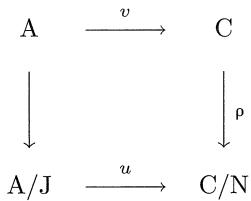
\includegraphics[keepaspectratio]{images/part001_bcdd9d30.jpg}}

where the vertical arrows represent the canonical surjections. We have \(v(\mathrm{J})\subset\mathrm{N}\), hence \(v(\mathrm{J}^{2})\subset\mathrm{N}^{2}=\{0\}\), and v defines, by passing to quotients, a homomorphism \(\bar{v}:\mathrm{A}/\mathrm{J}^{2}\to\mathrm{C}\) which satisfies \(\rho\circ\bar{v}=u\circ\pi\). Then \(\bar{v}\circ h\) is a lifting of u to C.

THEOREM 3.--- Let \(k\) be a ring, A a formally smooth \(k\)-algebra, and J a finitely generated ideal of A; set B=A/J.

\begin{enumerate}
\def\labelenumi{\alph{enumi})}
\tightlist
\item
  Let \(\mathfrak{p}\) be a prime ideal of B and let \(\mathfrak{q}\) be the (prime) ideal of A such that \(\mathfrak{p}=\mathfrak{q}/J\). The following conditions are equivalent:
\end{enumerate}

\begin{enumerate}
\def\labelenumi{(\roman{enumi})}
\item
  the k-algebra \(B_{\mathfrak{p}}\) is formally smooth;
\item
  there exists \(f\in B-\mathfrak{p}\) such that the k-algebra \(B_{f}\) is formally smooth;
\item
  the \(\kappa (\mathfrak{p})\)-linear map
\end{enumerate}

\[
\bar {d} _ {\kappa (\mathfrak {p})}: \kappa (\mathfrak {p}) \otimes_ {\mathrm{B}} \mathrm{J} / \mathrm{J} ^ {2} \rightarrow \kappa (\mathfrak {p}) \otimes_ {\mathrm{A}} \Omega_ {k} (\mathrm{A})
\]

is injective;

\begin{enumerate}
\def\labelenumi{(\roman{enumi})}
\setcounter{enumi}{3}
\tightlist
\item
  there exists an integer \(m \geqslant 0\) , elements \(f_{1}, \ldots, f_{m}\) of J, whose images \((f_{1})_{\mathfrak{q}}, \ldots, (f_{m})_{\mathfrak{q}}\) generate the ideal \(J_{\mathfrak{q}}\) , and k-derivations \(D_{1}, \ldots, D_{m}\) of A such that \(\det(\mathrm{D}_{j}(f_{i})) \not\in \mathfrak{q}\) .
\end{enumerate}

\begin{enumerate}
\def\labelenumi{\alph{enumi})}
\setcounter{enumi}{1}
\item
  The set of prime ideals p of B satisfying the equivalent conditions of (a) is open in Spec(B). For B to be formally smooth over k, it is necessary and sufficient that every prime (respectively maximal) ideal of B satisfy these conditions.
\item
  Suppose A is Noetherian. The conditions of (a) are also equivalent to:
\end{enumerate}

\begin{enumerate}
\def\labelenumi{(\alph{enumi})}
\setcounter{enumi}{21}
\tightlist
\item
  the k-algebra \(B_{\mathfrak{p}}\) is formally smooth for the topology \(\mathfrak{p}B_{\mathfrak{p}}\)-adic.
\end{enumerate}

Moreover, under the conditions of (iv), the ideal \(J_{\mathfrak{q}}\) is completely secant and the sequence \(((f_{1})_{\mathfrak{q}},\ldots,(f_{m})_{\mathfrak{q}})\) is completely secant for \(A_{\mathfrak{q}}\).

Set \(M = J/J^{2}\) and \(N = B \otimes_{A} \Omega_{k}(A)\) . The B-module \(M\) is of finite type, and the B-module \(N\) is projective ( \(n^{\circ} 5\) , cor. 3 of th. 2). For every multiplicative subset \(S\) of \(A\) , the \(k\) -algebra \(S^{-1}A\) is formally smooth ( \(n^{\circ} 2\) , prop. 4, a)). By lemma 4, conditions (i) and (ii) are therefore equivalent respectively to

(i') the map \(\bar{d}_{B_{\mathfrak{p}}}:M_{\mathfrak{p}}\longrightarrow N_{\mathfrak{p}}\) has a \(B_{\mathfrak{p}}\)-linear retraction;

(ii') there exists \(f \in \mathrm{B} - \mathfrak{p}\) such that the map \(\tilde{d}_{\mathrm{B}_f}: \mathrm{M}_f \to \mathrm{N}_f\) has a \(\mathrm{B}_f\)-linear retraction.

Prop. 9 of no. 8 applied to the ring B and to the homomorphism \(\bar{d}:M\to N\) implies the equivalence of conditions (i'), (ii'') and (iii), and also entails the assertions of (b) (using Lemma 4 again). Moreover, (iii) is equivalent to:

(iii') the map \(\kappa(\mathfrak{q})\otimes_{\mathrm{A}}\mathrm{J}\longrightarrow\kappa(\mathfrak{q})\otimes_{\mathrm{A}}\Omega_{k}(\mathrm{A})\) deduced from \(d:\mathrm{J}\to\Omega_{k}(\mathrm{A})\) is injective,

while (iv) can be written as:

(iv') there exists an integer \(m\geqslant 0\), elements \(f_{1},\ldots,f_{m}\) of J whose images generate the ideal \(J_{\mathfrak{q}}\) of \(A_{\mathfrak{q}}\), and elements \(y_{1},\ldots,y_{m}\) of \(\operatorname{Hom}_{\mathrm{A}}(\Omega_{k}(A),A)\) such that \(\det(\langle y_{j},df_{i}\rangle)\notin\mathfrak{q}\).

Since the \(\mathrm{A}\)-module \(\Omega_{k}(A)\) is projective (no. 5, cor. 3 of th. 2), prop. 9 of no. 8, applied to the ring A and to the homomorphism \(d:\mathrm{J}\to\Omega_{k}(A)\) provides the equivalence of (iii') and (iv').

Finally, suppose the ring A is Noetherian. It is clear that (i) implies (v). Under hypothesis (v), Lemma 3 implies that the map

\[
\bar {d} _ {\kappa (\mathfrak {q})}: \kappa (\mathfrak {q}) \otimes_ {\mathrm{B} _ {\mathfrak {p}}} \mathrm{J} _ {\mathfrak {q}} / \mathrm{J} _ {\mathfrak {q}} ^ {2} \longrightarrow \kappa (\mathfrak {q}) \otimes_ {\mathrm{A} _ {\mathfrak {q}}} \Omega_ {k} (\mathrm{A} _ {\mathfrak {q}})
\]

is injective, whence (iii).

Under the conditions of (iv), we have \(m=[\kappa(\mathfrak{q})\otimes_{\mathrm{A}}\mathrm{J}:\kappa(\mathfrak{q})]\) (no. 9, prop. 8). According to th. 2 of no. 5, the ideal \(J_{\mathfrak{q}}\) is completely secant, and the sequence \(((f_1)_{\mathfrak{q}},\ldots,(f_m)_{\mathfrak{q}})\) is completely secant for \(A_{\mathfrak{q}}\) (§ 1, no. 3, cor. 2 of th. 1). This proves c).

COROLLARY 1.--- Let \(k_{0}\) be a ring, \(k\) a Noetherian formally smooth \(k_{0}\)-algebra, and B a local \(k\)-algebra essentially of finite type. If the \(k_{0}\)-algebra B is formally smooth for the topology \(\mathfrak{m}_{\mathrm{B}}\)-adic, it is formally smooth.

There exists an integer \(n\geqslant 0\), a multiplicative subset S of \(k[\mathrm{T}_{1},\ldots,\mathrm{T}_{n}]\), and a surjective \(k\)-homomorphism \(\mathrm{S}^{-1}k[\mathrm{T}_{1},\ldots,\mathrm{T}_{n}]\to\mathrm{B}\). The algebra \(\mathrm{S}^{-1}k[\mathrm{T}_{1},\ldots,\mathrm{T}_{n}]\) is Noetherian and formally smooth over k (no. 3, Example 2 and no. 2, prop. 4, a)), hence over \(k_{0}\) (no. 2, prop. 3, a)). The corollary then follows from Theorem 3, c).

COROLLARY 2.--- Let \(k_{0}\) be a ring, \(k\) a Noetherian formally smooth \(k_{0}\)-algebra, and B a k-algebra essentially of finite type. The set U of prime ideals p of B such that the \(k_{0}\)-algebra \(B_{\mathfrak{p}}\) is formally smooth (for the discrete topology or the topology \(\mathfrak{p}B_{\mathfrak{p}}\)-adic) is open in Spec(B), and the following conditions are equivalent:

\begin{enumerate}
\def\labelenumi{(\roman{enumi})}
\item
  we have U = Spec(B);
\item
  U contains all the maximal ideals of B;
\item
  the \(k_{0}\)-algebra B is formally smooth.
\end{enumerate}

This follows as before from Theorem 3.

Note 1.--- Corollaries 1 and 2 apply in particular when \(k_{0}\) is a field and we are in one of the following two cases:

\begin{enumerate}
\def\labelenumi{\alph{enumi})}
\item
  B is an algebra essentially of finite type over a separable extension of \(k_{0}\) (th. 1 of no. 3);
\item
  B is a \(k_{0}\)-complete Noetherian local algebra whose residue field \(\kappa_{B}\) is a separable extension of \(k_{0}\) (in this case we take for k an algebra of formal power series over \(\kappa_{B}\) of which B is a quotient (no. 3 and IX, § 3, no. 3)).
\end{enumerate}

In each of these cases, it follows from Cor. 2, taking into account Prop. 8 of No. 7 and Prop. 6, b) of § 6, No. 4, that the \(k_0\)-algebra B is formally smooth if and only if it is absolutely regular.

COROLLARY 3 (Zariski). Let \(k\) be a field, A a \(k\)-local regular algebra, and J an ideal of A distinct from A. We assume that the \(k\)-algebra A is essentially of finite type or complete. For the local ring A/J to be regular, it is necessary and sufficient that there exists an integer \(m \geqslant 0\) , elements \(f_1, \ldots, f_m\) of J generating J and derivations D \(_1, \ldots, D_m\) of A such that det(D \(_j(f_i)\) ) \(\not\in \mathfrak{m}_{\mathrm{A}}\). The elements (f \(_1, \ldots, f_m\) ) then form part of a coordinate system of A and the ideal J is prime.

Let \(k_0\) be the prime subfield of \(k\). The \(k_0\)-algebra A is absolutely regular (§ 6, no. 4, Example 1), hence formally smooth (Remark 1 above). For the same reasons, saying that A/J is regular is equivalent to saying that it is a \(k_0\)-algebra formally smooth. The first assertion therefore follows from Theorem 3, which also implies that the sequence \((f_1,\ldots,f_m)\) is completely secant for A. One then applies Proposition 2 of VIII, § 5, no. 3.

Remark 2.--- Under the hypotheses of Cor. 3, the A-module \(\Omega(A)\) is projective (no. 5, Cor. 3 of Theorem 2), hence free; every derivation of A into \(\kappa_{A}\) therefore lifts to a derivation of A. The condition of the statement can thus be expressed as follows: there exists a generating system \((f_{1},\ldots,f_{m})\) of J and derivations \(D_{1},\ldots,D_{m}\) of A into \(\kappa_{A}\) , such that \(\det(D_{j}(f_{i}))\neq0\).

COROLLARY 4 (Zariski).--- Let k be a field and A a k-algebra essentially of finite type or a complete Noetherian local ring. The set of prime ideals p of A such that the local ring A \(_{p}\) is regular is open in Spec(A).

It suffices to apply Remark 1, taking for \(k_0\) the prime subfield of \(k\).

\subsection{Smooth algebras}

Lemma 5.--- Let \(\rho: A \to B\) be a local homomorphism of Noetherian local rings. Suppose that B is essentially of finite type over A. For the A-algebra B to be formally smooth, it is necessary and sufficient that the A-module B be flat and that the \(\kappa_{A}\)-algebra \(\kappa_{A} \otimes_{A} B\) be absolutely regular.

There exists an integer \(n \geqslant 0\), a prime ideal q of \(A[T_{1}, \ldots, T_{n}]\), and a surjective homomorphism h from \(A[T_{1}, \ldots, T_{n}]_{q}\) to B. Let C denote the local A-algebra \(A[T_{1}, \ldots, T_{n}]_{q}\); it is formally smooth ( \(n^{\circ} 3\), Example 2 and \(n^{\circ} 2\), Prop. 4, a)) and flat over A, and one may identify B with the A-algebra C/J, where \(J = \text{Ker}(h)\).

Set \(\overline{\mathrm{C}} = \kappa_{\mathrm{A}} \otimes_{\mathrm{A}} \mathrm{C}\) and \(\overline{\mathrm{B}} = \kappa_{\mathrm{A}} \otimes_{\mathrm{A}} \mathrm{B}\). Suppose B is formally smooth over A. The \(\kappa_{\mathrm{A}}\)-algebra \(\overline{\mathrm{B}}\) is then formally smooth (no. 2, prop. 4, b)), hence absolutely regular (no. 5, cor. 2 of th. 2). Moreover, since \(\overline{\mathrm{C}} / \overline{\mathrm{JC}}\) is identified with \(\overline{\mathrm{B}}\) and since the \(\kappa_{\mathrm{A}}\)-algebra \(\overline{\mathrm{C}}\) is formally smooth, the ideal \(\overline{\mathrm{JC}}\) of \(\overline{\mathrm{C}}\) is completely secant (no. 5, th. 2). It then follows from § 5, no. 6, prop. 6 that the A-module B is flat.

Suppose conversely that B is flat over A and that the \(\kappa_{\mathrm{A}}\)-algebra \(\overline{\mathbf{B}}\) is absolutely regular. Then the \(\kappa_{\mathrm{A}}\)-local algebra \(\overline{\mathbf{B}}\) is formally smooth (Remark 1 of no. 9 with \(k = k_0 = \kappa_{\mathrm{A}}\)). Set \(\overline{\mathbf{J}} = \kappa_{\mathrm{A}} \otimes_{\mathrm{A}} \mathrm{J}\); since B is a flat A-module, the canonical map \(\overline{\mathbf{J}} \to \overline{\mathbf{J}}\overline{\mathbf{C}}\) is bijective and \(\overline{\mathbf{B}}\) is identified with \(\overline{\mathbf{C}}/\overline{\mathbf{J}}\). It follows (Remark 1 of no. 2) that the canonical map

\[
\overline {{\mathrm{J}}} / \overline {{\mathrm{J}}} ^ {2} \longrightarrow \overline {{\mathrm{B}}} \otimes_ {\overline {{\mathrm{C}}}} \Omega_ {\kappa_ {\mathrm{A}}} (\overline {{\mathrm{C}}})
\]

is injective and admits a retraction. Now \(\overline{\mathrm{J}}/\overline{\mathrm{J}}^{2}\) is identified with \(\kappa_{\mathrm{A}}\otimes_{\mathrm{A}}\mathrm{J}/\mathrm{J}^{2}\), hence with \(\overline{\mathrm{B}}\otimes_{\mathrm{B}}\mathrm{J}/\mathrm{J}^{2}\). On the other hand, the \(\overline{\mathrm{C}}\)-module \(\Omega_{\kappa_{\mathrm{A}}}(\overline{\mathrm{C}})\) is canonically isomorphic to \(\overline{\mathrm{C}}\otimes_{\mathrm{C}}\Omega_{\mathrm{A}}(\mathrm{C})\) (A, III, p. 136, prop. 20), hence \(\overline{\mathrm{B}}\otimes_{\overline{\mathrm{C}}}\Omega_{\kappa_{\mathrm{A}}}(\overline{\mathrm{C}})\) is canonically isomorphic to \(\overline{\mathrm{B}}\otimes_{\mathrm{C}}\Omega_{\mathrm{A}}(\mathrm{C})\). Passing to the quotient by the maximal ideal of \(\overline{\mathrm{B}}\), one obtains an injective homomorphism

\[
\kappa_ {B} \otimes_ {B} J / J ^ {2} \longrightarrow \kappa_ {B} \otimes_ {C} \Omega_ {A} (C)
\]

which is precisely \(\bar{d}_{\kappa_{\mathrm{B}}}\). Thus B is formally smooth over A (th. 3).

THEOREM 4.--- Let A be a Noetherian ring and B an A-algebra essentially of finite type. The following conditions are equivalent:

\begin{enumerate}
\def\labelenumi{(\roman{enumi})}
\item
  the A-algebra B is formally smooth;
\item
  for every \(\mathfrak{q} \in \operatorname{Spec}(\mathrm{B})\) , the A-algebra \(\mathrm{B}_{\mathfrak{q}}\) is formally smooth (resp. formally smooth for the topology \(\mathfrak{q}\mathrm{B}_{\mathfrak{q}}\) -adic);
\item
  the A-module B is flat and, for every \(\mathfrak{p} \in \operatorname{Spec}(A)\) , the \(\kappa(\mathfrak{p})\) -algebra \(\kappa(\mathfrak{p}) \otimes_{A} B\) is absolutely regular;
\item
  the A-module B is flat and, for every regular A-algebra R, the ring R ⊗\_A B is regular;
\item
  the A-module B is flat and the kernel of the homomorphism \(\mu:B\otimes_{A}B\to B\) defined by \(\mu(x\otimes y)=xy\) is a completely secant ideal.
\end{enumerate}

The equivalence of (i) and (ii) follows from cor. 2 of th. 3 (no. 9).

(i)⇒(v): suppose the A-algebra B is formally smooth. Let q be a prime ideal of B, and let p be its inverse image in A. The \(A_{\mathfrak{p}}\)-algebra \(B_{\mathfrak{q}}\) is formally smooth (prop. 4, a) of no. 2), hence flat (Lemma 5); consequently the A-module B is flat (II, § 3, no. 4, prop. 15). On the other hand, the ring B ⊗A B is Noetherian (§ 6, no. 1, cor. of prop. 2), so the ideal Ker μ is completely secant by cor. 3 of th. 2 (no. 5).

(v)⇒(iii): suppose condition (v) is satisfied. Set I = Ker(μ). Let p ∈ Spec(A). The map

\[
1 \otimes \mu : \kappa (\mathfrak {p}) \otimes_ {\mathrm{A}} (\mathrm{B} \otimes_ {\mathrm{A}} \mathrm{B}) \rightarrow \kappa (\mathfrak {p}) \otimes_ {\mathrm{A}} \mathrm{B}
\]

is identified with the map

\[
\mu_ {\mathfrak {p}}: (\kappa (\mathfrak {p}) \otimes_ {\mathrm{A}} \mathrm{B}) \otimes_ {\kappa (\mathfrak {p})} (\kappa (\mathfrak {p}) \otimes_ {\mathrm{A}} \mathrm{B}) \rightarrow \kappa (\mathfrak {p}) \otimes_ {\mathrm{A}} \mathrm{B}
\]

deduced from the multiplication of the \(\kappa(\mathfrak{p})\) -algebra \(\kappa(\mathfrak{p})\otimes_{\mathrm{A}}\mathrm{B}\) . The ideal \(\operatorname{Ker}(\mu_{\mathfrak{p}})\) is identified with \(\mathrm{I}(\kappa(\mathfrak{p})\otimes_{\mathrm{A}}(\mathrm{B}\otimes_{\mathrm{A}}\mathrm{B}))\) . It is completely secant since the A-module B is flat ( \(\S 5\) , no. 6, prop. 6). Assertion (iii) then follows from prop. 8 of \(\S 6\) , no. 5.

(iii)⇒(ii): let q be a prime ideal of B, and p its inverse image in A. Under the hypotheses of (iii), the A \(_{p}\) -module B \(_{q}\) is flat, and the κ(p)-algebra κ(p) ⊗A \(_{p}\) B \(_{q}\) , which is identified with a ring of fractions of κ(p) ⊗A B, is absolutely regular (§ 6, no. 4, prop. 6). It follows from lemma 5 that B \(_{q}\) is formally smooth over A \(_{p}\) , hence over A (no. 2, prop. 3 and 4).

(iii)⇒(iv): let us place ourselves under the hypotheses of (iii). Let R be a regular A-algebra. The R-module R ⊗A B is flat (I, § 2, no. 7, cor. 2 to prop. 8). Let r be a prime ideal of R and p its inverse image in A; the ring κ(r)⊗R(R⊗AB), which is identified with κ(r)⊗κ(p) (κ(p)⊗A B), is regular (§ 6, no. 4, cor. 2 of prop. 7). The ring R ⊗A B is therefore regular (§ 4, no. 5, cor. of prop. 9).

(iv)⇒ (iii): let p be a prime ideal of A and let k be an extension of κ(p); under the hypotheses of (iv), the ring \(k \otimes_{\kappa(\mathfrak{p})} (\kappa(\mathfrak{p}) \otimes_{\mathrm{A}} \mathrm{B})\) , which is identified with \(k \otimes_{A} B\) , is regular, whence (iii).

DEFINITION 2.--- Let A be a Noetherian ring. An A-algebra B is said to be smooth if it is essentially of finite type and if it satisfies the equivalent conditions of Theorem 4.

PROPOSITION 10.--- Let A be a Noetherian ring.

\begin{enumerate}
\def\labelenumi{\alph{enumi})}
\item
  Let A' be a Noetherian A-algebra and B a smooth A-algebra. Then the A'-algebra A' ⊗\_A B is smooth.
\item
  Let B be a smooth A-algebra and C a smooth B-algebra. Then the A-algebra C is smooth.
\item
  Let B and C be two smooth A-algebras. Then the A-algebra B ⊗A C is smooth.
\end{enumerate}

This follows from prop. 4 of no. 2 and the analogous statements for algebras essentially of finite type (§ 6, no. 1).

Examples.--- 1) Smooth algebras over a field \(k\) are precisely the essentially finite-type and absolutely regular \(k\)-algebras.

\begin{enumerate}
\def\labelenumi{\arabic{enumi})}
\setcounter{enumi}{1}
\tightlist
\item
  Let A be a Noetherian ring, \(\mathbf{T} = (\mathrm{T}_i)_{i\in I}\) a finite family of indeterminates. The A-algebra A{[}T{]} is smooth. More generally, let \(\mathrm{F}_1,\ldots ,\mathrm{F}_m\) of elements of A{[}T{]}, and let B be the A-algebra A{[}T{]}/ \((\mathrm{F}_1,\dots ,\mathrm{F}_m)\). If in every maximal ideal \(\mathfrak{n}\) of B the class (mod. \(\mathfrak{n}\) ) of the matrix \(\left(\frac{\partial\mathrm{F}_j}{\partial\mathrm{T}_i}\right)\) is of rank \(m\) , the A-algebra B is smooth (th. 3 of no. 9).
\end{enumerate}

\section{Duality of modules of finite length}

\subsection{Indecomposable injective modules}

Let A be a ring. The relation “I is a class of indecomposable injective A-modules” is collectivizing (A, X, p. 21, cor. 1); we shall denote by \(\mathcal{I}(A)\) the set of classes of indecomposable injective A-modules.

PROPOSITION 1.--- Let A be a Noetherian ring. For every prime ideal p of A, let \(e_{\mathfrak{p}}: \mathrm{A}/\mathfrak{p} \to \mathrm{I}(\mathfrak{p})\) be an injective envelope of \(\mathrm{A}/\mathfrak{p}\) (A, X, § 1, no. 9).

\begin{enumerate}
\def\labelenumi{\alph{enumi})}
\item
  The A-modules I(p) are indecomposable.
\item
  Let I be an indecomposable injective A-module; the set Ass(I) is reduced to a single element.
\item
  The map \(\mathfrak{p} \mapsto \operatorname{cl}(\operatorname{I}(\mathfrak{p}))\) is a bijection of \(\operatorname{Spec}(\operatorname{A})\) onto \(\mathcal{I}(A)\). The inverse bijection associates to an element I of \(\mathcal{I}(\operatorname{A})\) the unique element of \(\operatorname{Ass}(\operatorname{I})\).
\end{enumerate}

Let \(\mathfrak{p} \in \operatorname{Spec}(A)\); let us prove that the module \(I(\mathfrak{p})\) is indecomposable. By A, X, p. 21, cor. 2, it suffices to prove that if \(\mathfrak{a}\) and \(\mathfrak{b}\) are ideals of A containing \(\mathfrak{p}\) and distinct from \(\mathfrak{p}\), the ideal \(\mathfrak{a} \cap \mathfrak{b}\) is distinct from \(\mathfrak{p}\) ; or if \(a\) is an element of \(\mathfrak{a} - \mathfrak{p}\) and \(b\) is an element of \(\mathfrak{b} - \mathfrak{p}\) the product \(ab\) belongs to \((\mathfrak{a} \cap \mathfrak{b}) - \mathfrak{p}\).

Let I be an indecomposable injective A-module, and let p, q be elements of Ass(I). Then I contains a submodule M isomorphic to A/p and a submodule N isomorphic to A/q. We have M ∩ N ≠ 0 (A, X, p. 21, prop. 14); for every nonzero element x of M ∩ N, we have p = Ann x = q. Since Ass(I) is not empty (IV, § 1, n° 1, cor. 1 of prop. 2), it is reduced to a single element p(I).

We have thus defined two maps. \(\mathfrak{p} \mapsto \operatorname{cl}(I(\mathfrak{p}))\) of \(\operatorname{Spec}(A)\) in \(\mathcal{I}(A)\) and \(I \mapsto \mathfrak{p}(I)\) of \(\mathcal{I}(A)\) in \(\operatorname{Spec}(A)\); let us prove that these two maps are inverse bijections of each other. Let \(\mathfrak{p} \in \operatorname{Spec}(A)\) ; then \(\mathfrak{p}\) belongs to \(\operatorname{Ass}(I(\mathfrak{p}))\), and it is therefore the unique element of \(\operatorname{Ass}(I(\mathfrak{p}))\). Let \(I\) be an indecomposable injective A-module, and \(\mathfrak{p}\) the unique element of \(\operatorname{Ass}(I)\) ; then \(I\) is an injective envelope of \(A/\mathfrak{p}\) (A, X, p. 21, prop. 14). This completes the proof of the proposition.

Remark 1.—Let I be an indecomposable injective A-module, and let p be the unique element of Ass(I); by Prop. 1, I contains a submodule isomorphic to A/p of which it is an injective envelope. In general such a submodule is not unique, as one sees by taking A = Z, p = 0, I = Q.

For every prime ideal \(\mathfrak{p}\) of \(\mathrm{A}\), let us choose, as above, an injective envelope \((\mathrm{I}(\mathfrak{p}), e_{\mathfrak{p}})\) of \(\Lambda/\mathfrak{p}\). By \(\mathrm{A}\), X, p. 22, th. 3, we have:

THEOREM 1.--- Let A be a Noetherian ring. For every injective A-module I, there exists one and only one family of cardinals \((a_{\mathfrak{p}})_{\mathfrak{p}\in\operatorname{Spec}(\mathrm{A})}\), such that I is isomorphic to \(\bigoplus_{\mathfrak{p}}\mathrm{I}(\mathfrak{p})^{(a_{\mathfrak{p}})}\).

By IV, § 1, no. 1, cor. 1 of prop. 3, the set Ass(I) is then the support of the family \((a_{\mathfrak{p}})\) .

Remark 2. Let \(A\) be a Noetherian ring, M an A-module, \(e: \mathrm{M} \to \mathrm{I}\) an injective envelope of M. The set Ass(M) is equal to Ass(I): indeed, the inclusion Ass(M) ⊂ Ass(I) is evident. On the other hand, if \(\mathfrak{p}\) is an element of Ass(I), I contains a submodule N isomorphic to \(A/\mathfrak{p}\) ; since the \(A\)-module \(e^{-1}(\mathrm{N})\) is nonzero, we have \(\operatorname{Ass}(e^{-1}(\mathrm{N})) = \{\mathfrak{p}\}\). This proves that \(\mathfrak{p}\) is associated with \(e^{-1}(\mathrm{N})\), hence to M, whence our assertion.

Let us adopt the notation of the theorem, and suppose moreover that Ass(M) is finite. For every \(\mathfrak{q} \in \operatorname{Ass}(M)\) let us denote by \(Q_{\mathfrak{q}}\) the intersection with M of \(\bigoplus_{\mathfrak{p} \in \operatorname{Ass}(M) - \{\mathfrak{q}\}} I(\mathfrak{p})^{(a_{\mathfrak{p}})}\). Then \((Q_{\mathfrak{q}})_{\mathfrak{q} \in \operatorname{Ass}(M)}\) is a reduced primary decomposition of 0 in M (IV, § 2, n° 3, def. 3). Indeed, we have \(\cap Q_{\mathfrak{q}} = 0\); as \(M/Q_{\mathfrak{q}}\) is identified with a nonzero submodule of \(I(\mathfrak{q})^{(a_{\mathfrak{q}})}\), one has \(\operatorname{Ass}(M/Q_{\mathfrak{q}}) = \{\mathfrak{q}\}\) and it suffices to apply prop. 4 of loc. cit.

Example.--- Let A be a principal ideal ring, and let K be its field of fractions. The injective A-modules are the divisible A-modules (A, X, p. 17, cor. 2). The A-module K is an injective envelope of A (A, X, p. 20, example 1). Let \(p\) be an extremal element of A, and \(\mathfrak{p}\) the (maximal) ideal \(Ap\). Let us denote by \(e: A/\mathfrak{p} \longrightarrow K/A_{\mathfrak{p}}\) the homomorphism that maps the class of an element \(a \in A\) to the class of \(a/p\). Let us prove that \((K/A_{\mathfrak{p}}, e)\) is an injective envelope of \(A/\mathfrak{p}\). The homomorphism \(e\) is injective. The A-module \(K/A_{\mathfrak{p}}\) is a quotient of a divisible module, hence is divisible. Let \(x\) be a nonzero element of \(K/A_{\mathfrak{p}}\) ; it is the class of an element \(a/p^n\) of K, with \(a \in A - \{0\}\) and \(n \geqslant 1\) (A, VII, p. 10, th. 2). We then have \(p^{n-1}x = e(a)\) , hence \(e(Ax) \neq 0\), which proves our assertion.

It then follows from th. 1 that every divisible A-module is a direct sum of A-modules isomorphic to K or to \(K/A_{p}\) for a maximal (principal) ideal p of A.

\subsection{Structure of indecomposable injective modules}

Lemma 1.--- Let A be a ring, with a an ideal of A, and I an A-module. For every integer \(n \geqslant 0\) let us denote by \(I_{n}\) the submodule of I consisting of the elements annihilated by \(a^{n}\).

\begin{enumerate}
\def\labelenumi{\alph{enumi})}
\item
  Suppose the A-module I is injective. Then the \(\mathrm{A} / \mathfrak{a}^n\)-module \(\mathrm{I}_n\) is injective for every \(n \geqslant 0\).
\item
  Suppose that the ring A is Noetherian, and that for every \(n \geqslant 0\) the \(\mathrm{A} / \mathfrak{a}^n\) -module \(\mathrm{I}_n\) be injective. Then the union of the \(\mathrm{I}_n\) is an injective A-module.
\item
  The \(\mathbf{A} / \mathfrak{a}^n\) -module \(\mathrm{I}_n\) is isomorphic to \(\operatorname{Hom}_{\mathbf{A}}(\mathbf{A} / \mathfrak{a}^n, \mathbf{I})\), which is injective (A, X, p. 18, prop. 11).
\item
  Let J be the union of the \(I_{n}\), b an ideal of A, and \(f : b \to J\) an A-homomorphism. It remains (A, X, p. 16, prop. 10) of proving that there exists an element x of J such that one has \(f(b) = bx\) for every \(b \in b\). Since b is of finite type, there exists an integer n such that one has \(f(\mathfrak{b}) \subset \mathrm{I}_{n}\) , that is \(f(\mathfrak{a}^{n}\mathfrak{b}) = 0\) . According to cor. 2 of prop. 1 of III, § 3, no. 1, there exists an integer \(m \geqslant n\) such that \(a^{m} \cap b \subset a^{n}b\) , hence \(f(\mathfrak{a}^{m} \cap \mathfrak{b}) = 0\) . Then f induces an A/\(a^{m}\)-linear homomorphism from \(\mathfrak{b}/(\mathfrak{a}^{m} \cap \mathfrak{b})\) into \(I_{m}\); since the A/ \(a^{m}\)-module \(I_{m}\) is injective, there exists an element x of \(I_{m}\) such that one has \(f(b) = bx\) for every \(b \in b\) , whence b).
\end{enumerate}

Let \(\mathfrak{a}\) be an ideal of A; in what follows we shall agree to set \(\mathfrak{a}^n = \mathrm{A}\) for every integer \(n \leqslant 0\). Let E be an A-module. For every \(n \in \mathbf{Z}\) let us denote by \(\mathrm{E}_n\) the submodule of E consisting of the elements annihilated by \(\mathfrak{a}^n\); let \(\mathrm{gr}^{\mathfrak{a}}(\mathrm{E})\) be the graded A-module of type \(\mathbf{Z}\) such that \(\mathrm{gr}^{\mathfrak{a}}(\mathrm{E})_m = \mathrm{E}_{-m+1}/\mathrm{E}_{-m}\) for every integer \(m\). The module \(\mathrm{gr}^{\mathfrak{a}}(\mathrm{E})_m\) is zero for \(m \geqslant 1\) , and \(\mathrm{gr}^{\mathfrak{a}}(\mathrm{E})_0\) is identified with \(\mathrm{E}_1\) . Let \(\mathrm{gr}(\mathrm{A})\) be the associated graded ring of A for the \(\mathfrak{a}\) -adic filtration: we have \(\mathrm{gr}(\mathrm{A})_n = \mathfrak{a}^n/\mathfrak{a}^{n+1}\) for every \(n \in \mathbf{Z}\). Let \(n\) and \(m\) be integers. By passing to quotients of the bilinear map \((a,x) \mapsto ax\) of \(\mathfrak{a}^n \times \mathrm{E}_{-m+1}\) in \(\mathrm{E}_{-m-n+1}\) we deduce an A/ \(\mathfrak{a}\) -bilinear map

\[
\alpha_ {n, m}: \mathrm{gr} (\mathrm{A}) _ {n} \times \mathrm{gr} ^ {\mathfrak {a}} (\mathrm{E}) _ {m} \longrightarrow \mathrm{gr} ^ {\mathfrak {a}} (\mathrm{E}) _ {n + m},\tag{1}
\]

which defines on gr \(^{a}\) (E) a graded gr(A)-module structure. For every \(n \in \mathbf{Z}\) one deduces from the A/a-bilinear map \(\alpha_{n,-n} : \text{gr}(A)_n \times \text{gr}^{a}(E)_{-n} \longrightarrow E_1\) an A/a-linear map \(\beta_{E,n} : \text{gr}^{a}(E)_{-n} \longrightarrow \text{Hom}_{A/\alpha}(\text{gr}(A)_n, E_1)\); the maps \(\beta_{E,n}\) are the components of a homomorphism of graded A/a-modules, called canonical.

\[
\beta_ {\mathrm{E}}: \operatorname{gr} ^ {a} (\mathrm{E}) \longrightarrow \operatorname{Homgr} _ {\mathrm{A} / \mathfrak{a}} (\operatorname{gr} (\mathrm{A}), \mathrm{E} _ {1}).\tag{2}
\]

For \(a \in \text{gr(A)}\), \(x \in \text{gr}^{\mathfrak{a}}(\text{E})\) , \(\beta_{\text{E}}(x)(a)\) is by definition the component in \(\text{gr}^{\mathfrak{a}}(\text{E})_0 = \text{E}_1\) of the element \(ax\) of \(\text{gr}^{\mathfrak{a}}(\text{E})\). It follows that \(\beta_{\text{E}}\) is \(\text{gr(A)}\) -linear when one equips \(\text{Homgr}_{\text{A}/\mathfrak{a}}(\text{gr(A)}, \text{E}_1)\) with the structure of \(\text{gr(A)}\) -module defined by the formula \((bf)(a) = f(ab)\) for \(a, b\) in \(\text{gr(A)}\) and \(f\) in \(\text{Homgr}_{\text{A}/\mathfrak{a}}(\text{gr(A)}, \text{E}_1)\) .

PROPOSITION 2.--- Let A be a Noetherian ring, with a an ideal of A, E an A-module, and M a sub-A-module of E annihilated by a. The following conditions are equivalent:

\begin{enumerate}
\def\labelenumi{(\roman{enumi})}
\item
  E is an injective envelope of M;
\item
  the \(\mathrm{A}/\mathfrak{a}\)-module \(\mathrm{E}_1\) is an injective envelope of the \(\mathrm{A}/\mathfrak{a}\) -module \(\mathrm{M}\); the module \(\mathrm{E}\) is the union of \(\mathrm{E}_n\), and the canonical map \(\beta_{\mathrm{E}}\) is bijective.
\end{enumerate}

Suppose condition (i) is satisfied. The A/a-module \(E_{1}\) is injective (Lemma 1, a)), and contains M; since every sub- \(A/a\) -module of \(E_{1}\) is a sub-A-module of E, \(E_{1}\) is an injective envelope of the A/a-module M. By Lemma 1, the union of the \(E_{n}\) is an injective sub-A-module of E containing M, hence equal to E. Since E is injective, we have for all \(n \geqslant 0\) an exact sequence

\[
0 \to \operatorname{Hom} _ {\mathrm{A}} (\mathrm{A} / \mathfrak {a} ^ {n}, \mathrm{E}) \longrightarrow \operatorname{Hom} _ {\mathrm{A}} (\mathrm{A} / \mathfrak {a} ^ {n + 1}, \mathrm{E}) \longrightarrow \operatorname{Hom} _ {\mathrm{A}} (\mathfrak {a} ^ {n} / \mathfrak {a} ^ {n + 1}, \mathrm{E}) \to 0;
\]

as \(\mathrm{Hom}_{\mathrm{A}}(\mathrm{A}/\mathfrak{a}^{m},\mathrm{E})\) is identified with \(\mathrm{E}_{m}\) for every \(m\) and that the canonical injection of \(\mathrm{Hom}_{\mathrm{A}}(\mathfrak{a}^{n}/\mathfrak{a}^{n+1},\mathrm{E}_{1})\) in \(\mathrm{Hom}_{\mathrm{A}}(\mathfrak{a}^{n}/\mathfrak{a}^{n+1},\mathrm{E})\) is bijective, we deduce that the canonical homomorphism \(\beta_{\mathrm{E}}\) is bijective, whence (ii).

Suppose (ii) is satisfied. Let \(e: \mathrm{M} \to \mathrm{I}\) be an injective envelope of M. Since I is injective, there exists an A-linear map \(\varphi: \mathrm{E} \to \mathrm{I}\) extending \(e\). But \(\varphi\) maps \(\mathrm{E}_n\) in \(\mathrm{I}_n\) for every \(n\), therefore induces homomorphisms \(\mathrm{gr}^{\mathfrak{a}}(\varphi):\mathrm{gr}^{\mathfrak{a}}(\mathrm{E})\to \mathrm{gr}^{\mathfrak{a}}(\mathrm{I})\) and \(\varphi_{1}:\mathrm{E}_{1}\rightarrow \mathrm{I}_{1}\) thereby making the diagram commutative

\[
\begin{array}{c c c} \operatorname{gr} ^ {\mathfrak {a}} (\mathrm{E}) & \xrightarrow {\beta_ {\mathrm{E}}} & \operatorname{Homgr} _ {\mathrm{A} / \mathfrak {a}} (\operatorname{gr} (\mathrm{A}), \mathrm{E} _ {1}) \\ \operatorname{gr} ^ {\mathfrak {a}} (\varphi) \Bigg \downarrow & & \Bigg \downarrow \operatorname{Homgr} (1, \varphi_ {1}) \\ \operatorname{gr} ^ {\mathfrak {a}} (\mathrm{I}) & \xrightarrow {\beta_ {\mathrm{I}}} & \operatorname{Homgr} _ {\mathrm{A} / \mathfrak {a}} (\operatorname{gr} (\mathrm{A}), \mathrm{I} _ {1}). \end{array}
\]

Since \(E_{1}\) and \(I_{1}\) are injective envelopes of the A/a-module M, the homomorphism \(\varphi_{1}\) is bijective; since \(\beta_{E}\) and \(\beta_{I}\) are bijective, it follows that \(\mathrm{gr}^{\mathfrak{a}}(\varphi)\) is bijective. This implies, by induction on n, that \(\varphi\) induces a bijection from \(E_{n}\) onto \(I_{n}\) for every \(n \geqslant 1\); therefore \(\varphi\) is bijective, which implies (i).

Lemma 2.--- Let A be a ring, let a be a finitely generated ideal of A, and let M be an A-module in which every element is annihilated by a power of a. Let A-hat denote the separated completion of A for the a-adic topology.

\begin{enumerate}
\def\labelenumi{\alph{enumi})}
\item
  There exists on M a unique structure of \(\widehat{\mathrm{A}}\) -module extending the given structure of A-module.
\item
  The sub-A-hat-modules of M are its sub-A-modules, and one has Hom \(_{\text{A}}\) (M, P) = Hom \(_{\widehat{\text{A}}}\) (M, P) for every \(\widehat{\text{A}}\) -module P.
\item
  Identify \(\widehat{\mathbf{A}}\) with the projective limit of the rings \(\mathrm{A} / \mathfrak{a}^n\), and endow M with the discrete topology. Let \(a = (a_n)\) be an element of \(\widehat{\mathbf{A}}\) , and let \(x\) an element of M. Since \(x\) is annihilated by a power of \(\mathfrak{a}\) , the sequence \((a_n x)\) is stationary; denote its limit by \(ax\). The map \((a, x) \mapsto ax\) defines on M a structure of \(\widehat{\mathbf{A}}\) -module which extends the given structure of A-module.
\end{enumerate}

Conversely, suppose such a structure on M is given; let \(a = (a_{n})\) be an element of \(\widehat{\mathrm{A}}\), \(x\) be an element of M and \(m\) an integer such that \(\mathfrak{a}^{m}x = 0\). For every integer \(n\) , \(a - a_{n}\) belongs to \(\widehat{\mathfrak{a}^{n}}\) , which is equal to \(\mathfrak{a}^{n}\widehat{\mathrm{A}}\) (III, § 2, n° 12, cor. 2 of prop. 16); one therefore has \(ax = a_{n}x\) for \(n \geqslant m\) , whence the uniqueness assertion.

\begin{enumerate}
\def\labelenumi{\alph{enumi})}
\setcounter{enumi}{1}
\tightlist
\item
  It follows from the preceding that one has \(Ax = \widehat{A}x\) for every \(x \in M\) ; the sub- \(\widehat{A}\)-modules of \(M\) are therefore its sub- \(A\) -modules. Finally, let \(u\) be an \(A\)-linear homomorphism from \(M\) into a \(\widehat{A}\) -module \(P\). Let \(a = (a_n)\) be an element of \(\widehat{A}\) , \(x\) be an element of \(M\) and \(m\) an integer such that \(\mathfrak{a}^m x = 0\) ; one has \(\mathfrak{a}^m u(x) = 0\) . Since \(a - a_m\) belongs to \(\mathfrak{a}^m\widehat{A}\) , one has
\end{enumerate}

\[
u (a x) = u \left(a _ {m} x\right) = a _ {m} u (x) = a u (x),
\]

so that u is A-hat-linear.

PROPOSITION 3. Let A be a Noetherian ring, p a prime ideal of A and e : A/p → I an injective envelope of the A-module A/p. For every integer n ≥ 0, denote by I \(_{n}\) the submodule of I consisting of the elements annihilated by p \(^{n}\).

\begin{enumerate}
\def\labelenumi{\alph{enumi})}
\item
  The A-module I is the union of the \(I_{n}\). The injection \(\Lambda/p \to I_{1}\) extends to an isomorphism from \(\kappa(\mathfrak{p})\) onto \(I_{1}\); identify \(\kappa(\mathfrak{p})\) with \(I_{1}\) by means of this isomorphism. For each integer \(n \geqslant 0\) , the structure of \(\Lambda/p\)-module on \(I_{n+1}/I_{n}\) comes by restriction of scalars from a unique structure of \(\kappa(\mathfrak{p})\) -vector space; the canonical homomorphism \(\beta_{I,-n}: I_{n+1}/I_{n} \longrightarrow \operatorname{Hom}_{\mathrm{A}/\mathfrak{p}}(\mathfrak{p}^{n}/\mathfrak{p}^{n+1}, \kappa(\mathfrak{p}))\) is an isomorphism of \(\kappa(\mathfrak{p})\) -vector spaces of finite dimension.
\item
  There exists a unique structure of \(\mathrm{A_p}\) -module on I inducing its structure of A-module. The canonical homomorphism \(\widehat{\mathrm{A_p}} \longrightarrow \mathrm{End}_{\mathrm{A}}(\mathrm{I})\) is bijective.
\end{enumerate}

By A, X, p. 20, example 1, the A/p-module \(\kappa(\mathfrak{p})\) is an injective envelope of A/p. It therefore follows from prop. 2 that I \(_1\) is identified with \(\kappa(\mathfrak{p})\), that I is the union of the I \(_m\) , and for every integer \(n \geqslant 0\) , \(\beta_{1,-n}\) is an isomorphism of A/p-modules. For every nonzero element \(a\) of A/p, the homothety with ratio \(a\) is invertible in Hom \(_{\text{A/p}}(\mathfrak{p}^n/\mathfrak{p}^{n+1}, \kappa(\mathfrak{p}))\) , hence also in I \(_{n+1}\) /I \(_n\) , which completes the proof of a).

Let \(s \in A - p\). Since the homothety \(s_{A/p}\) is injective, the trace of Ker \(s_I\) on \(A/p\) is zero, which implies that the homothety \(s_I\) is injective. Then \(sI\) is a direct summand of I (A, X, p. 19, cor. 4), hence equal to I since I is indecomposable ( \(n^o\) 1, prop. 1), so that the homothety \(s_I\) is bijective. There therefore exists a unique structure of \(A_p\) -module on I inducing its structure of A-module; it extends uniquely to a structure of \(\widehat{A_p}\) -module (lemma 2).

For every integer \(n\) , we deduce from the canonical ring homomorphism \(\Lambda_{\mathfrak{p}} \longrightarrow \mathrm{End}_{\mathrm{A}}(\mathrm{I})\) an A-linear map \(\alpha_{n}: \mathrm{A}_{\mathfrak{p}}/\mathfrak{p}^{n}\mathrm{A}_{\mathfrak{p}} \longrightarrow \mathrm{Hom}_{\mathrm{A}}(\mathrm{I}_{n},\mathrm{I})\). Consider the commutative diagram with exact rows

\[
\begin{array}{c c c c c c c c c} 0 & \longrightarrow & \mathfrak {p} ^ {n} A _ {\mathfrak {p}} / \mathfrak {p} ^ {n + 1} A _ {\mathfrak {p}} & \longrightarrow & A _ {\mathfrak {p}} / \mathfrak {p} ^ {n + 1} A _ {\mathfrak {p}} & \longrightarrow & A _ {\mathfrak {p}} / \mathfrak {p} ^ {n} A _ {\mathfrak {p}} & \longrightarrow & 0 \\ & & \alpha_ {n + 1} ^ {\prime} \Bigg \downarrow & & \alpha_ {n + 1} \Bigg \downarrow & & \alpha_ {n} \Bigg \downarrow \\ 0 & \longrightarrow & \operatorname{Hom} _ {A} (I _ {n + 1} / I _ {n}, I _ {1}) & \longrightarrow & \operatorname{Hom} _ {A} (I _ {n + 1}, I) & \longrightarrow & \operatorname{Hom} _ {A} (I _ {n}, I) & \longrightarrow & 0 \end{array}
\]

where \(\alpha_{n+1}^{\prime}\) is the homomorphism induced by \(\alpha_{n+1}\). Consider the canonical \(\kappa(\mathfrak{p})\)-bilinear map

\[
\alpha_ {n, - n}: \mathfrak {p} ^ {n} \mathrm{A} _ {\mathfrak {p}} / \mathfrak {p} ^ {n + 1} \mathrm{A} _ {\mathfrak {p}} \times \mathrm{I} _ {n + 1} / \mathrm{I} _ {n} \longrightarrow \mathrm{I} _ {1}
\]

(formula (1)). The linear map \(I_{n+1}/I_{n} \longrightarrow \operatorname{Hom}_{\kappa(\mathfrak{p})}(\mathfrak{p}^{n}A_{\mathfrak{p}}/\mathfrak{p}^{n+1}A_{\mathfrak{p}}, I_{1})\) associated with it on the left is identified with \(\beta_{I,-n}\), and the one associated with it on the right is \(\alpha_{n+1}'\) . Since \(\beta_{I,-n}\) is bijective by a), and the same holds for \(\alpha_{n+1}'\); it follows from the above diagram, by induction on n, that \(\alpha_{n}\) is an isomorphism for every n. Since I is the union of the \(I_{n}\) , the canonical map \(\operatorname{End}_{\mathrm{A}}(\mathrm{I}) \to \varprojlim \operatorname{Hom}_{\mathrm{A}}(\mathrm{I}_{n}, \mathrm{I})\) is bijective; the ring homomorphism \(\widehat{A_{p}} \to \operatorname{End}_{\mathrm{A}}(\mathrm{I})\) which is identified with the projective limit of the maps \(\alpha_{n}\) is therefore bijective.

Remark.--- It follows from the preceding proof that the annihilator of \(I_{n}\) in \(\widehat{A_{p}}\) (resp. in \(A_{p}\) ) is \(p^{n}\widehat{A_{p}}\) (resp. \(p^{n}A_{p}\) ). Consequently, the annihilator of the A-module \(I_{n}\) is the inverse image in A of the ideal \(p^{n}A_{p}\) which is sometimes denoted \(\mathfrak{p}^{(n)}\) which is called the n-th symbolic power of the prime ideal p.

COROLLARY.--- Let J be an injective A-module such that \(\mathrm{Ass}_{\mathrm{A}}(\mathrm{J}) = \{\mathfrak{p}\}\).

\begin{enumerate}
\def\labelenumi{\alph{enumi})}
\item
  \(L^{\prime}\) canonical map \(\mathrm{J} \to \mathrm{A}_{\mathfrak{p}} \otimes_{\mathrm{A}} \mathrm{J}\) is bijective.
\item
  Let E denote the A/p-module Hom \(_A\) (A/p, J). On E there exists a unique structure of \(\kappa(p)\)-vector space extending its structure as an A/p-module; the A-module J is isomorphic to I \(^{([E:\kappa(p)])}\).
\end{enumerate}

Indeed, J is isomorphic to an A-module \(I^{(\mathfrak{c})}\) , where c is a suitable cardinal (no. 1, th. 1). The corollary follows from the proposition when J = I, and the general case is deduced from it immediately.

\subsection{Matlis duality}

In this section, we assume that the ring A is local Noetherian.

DEFINITION.--- An A-module I is said to be a Matlis A-module if it is injective, if \(\mathfrak{m}_{\mathrm{A}}\) is its unique associated prime ideal and if the \(\kappa_{\mathrm{A}}\) -vector space \(\operatorname{Hom}_{\mathrm{A}}(\kappa_{\mathrm{A}}, \mathrm{I})\) has dimension 1.

Let \(e: \kappa_{\mathrm{A}} \to I\) be an injective envelope of \(\kappa_{\mathrm{A}}\) (A, X, p. 20, th. 2). The A-module I is a Matlis module, and every Matlis A-module is isomorphic to I (no. 2, cor. of prop. 3). If A is a discrete valuation ring with field of fractions K, the A-module K/A is a Matlis module (no. 1, example). If A is a local Artinian ring, the A-module A is a Matlis module if and only if A is a Gorenstein ring (§ 3, no. 7, lemma 1).

Let I be a Matlis A-module. For every integer \(n \geqslant 0\) let us denote by \(I_n\) the sub-A-module of I consisting of the elements annihilated by \(\mathfrak{m}_A^n\) . By prop. 2 of no. 2, the A-module I is the union of the \(I_n\), the A-module \(I_1\) is of length 1 (that is, isomorphic to \(\kappa_A\) ) and the A-module I is an injective envelope of \(I_1\); moreover, the canonical homomorphism of graded gr(A)-modules

\[
\beta : \mathrm{gr} ^ {\mathrm{m} _ {\mathrm{A}}} (\mathrm{I}) \longrightarrow \operatorname{Homgr} _ {\kappa_ {\mathrm{A}}} (\mathrm{gr} (\mathrm{A}), \mathrm{I} _ {1})\tag{3}
\]

is an isomorphism. By prop. 3 of no. 2, the A-module structure of I extends uniquely to a structure of \(\widehat{\mathrm{A}}\) -module, and the canonical homomorphism \(\widehat{\mathrm{A}} \to \operatorname{End}_{\mathrm{A}}(\mathrm{I})\) is bijective.

Lemma 3.-- Let I be a Matlis A-module. Then:

\begin{enumerate}
\def\labelenumi{\alph{enumi})}
\item
  I is a A-hat-Matlis module;
\item
  the A-module I is Artinian and a cogenerator (A, X, p. 18, def. 3).
\end{enumerate}

Since the A-module I is injective, the \(\mathbf{A} / \mathfrak{m}_{\mathbf{A}}^{n}\) -module \(\mathrm{I}_n\) is injective for each \(n\) ( \(n^{\circ}2\), (lemma 1, a)). Since \(\mathrm{I}_n\) is the set of elements of I annihilated by \(\mathfrak{m}_{\widehat{\mathrm{A}}}^{n}\) , the \(\widehat{\mathrm{A}}\) -module I is injective (lemma 1, b)). It is indecomposable over \(\widehat{\mathrm{A}}\) since it is so over \(\mathrm{A}\); as it contains the sub- \(\widehat{\mathrm{A}}\) -module \(\mathrm{I}_1\) isomorphic to \(\kappa_{\mathrm{A}}\) , one has \(\mathfrak{m}_{\widehat{\mathrm{A}}} \in \operatorname{Ass}_{\widehat{\mathrm{A}}}(\mathrm{I})\) , hence \(\operatorname{Ass}_{\widehat{\mathrm{A}}}(\mathrm{I}) = \{\mathfrak{m}_{\widehat{\mathrm{A}}}\}\) (prop. 1), whence a).

Let us now prove that I is Artinian. To every sub-A-module M of I, associate the graded ideal \(\mathfrak{a}_{\mathrm{M}}\) of gr(A) defined as follows: an element of gr(A) \(_n\) belongs to \((\mathfrak{a}_{\mathrm{M}})_{n}\) if it is annihilated by all the linear forms \(\boldsymbol{\beta}(x)\), where x ranges over \(\left((\mathrm{M}\cap\mathrm{I}_{n+1})+\mathrm{I}_{n}\right)/\mathrm{I}_{n}\). Let M and N be submodules of I such that \(N\subset M\); one has \(a_{M}\subset a_{N}\) . Suppose \(a_{M}=a_{N}\) ; one has \((M\cap I_{n+1})+I_{n}=(N\cap I_{n+1})+I_{n}\) for all n since \(\beta\) is an isomorphism. By induction on n we deduce \(M\cap I_{n+1}=N\cap I_{n+1}\) for all n, whence finally M=N.

That being so, let \(M_{0} \supset M_{1} \supset \ldots \supset M_{n} \supset \ldots\) be a decreasing sequence of sub-A-modules of I; the increasing sequence \(a_{M_{0}} \subset a_{M_{1}} \subset \ldots\) is stationary, since \(\text{gr}(A)\) is an \(\kappa_{A}\) -algebra of finite type. The sequence \((M_{i})_{i \geqslant 0}\) is therefore stationary, which implies that the A-module I is Artinian. Finally, the A-module I is a cogenerator by virtue of A, X, p. 18, prop. 12.

Let M be an A-module. Recall (A, VIII, § 4, n° 6) that the socle of M is the sum of the simple submodules of M, that is, the set of elements of M annihilated by \(\mathfrak{m}_{\mathrm{A}}\); it is a \(\kappa_{\mathrm{A}}\) -vector space, canonically isomorphic to \(\operatorname{Hom}_{\mathrm{A}}(\kappa_{\mathrm{A}}, \mathrm{M})\).

Lemma 4. Let I be a Matlis module over A and let M be an \(A\)-module. The following conditions are equivalent:

\begin{enumerate}
\def\labelenumi{(\roman{enumi})}
\item
  M is Artinian;
\item
  every element of M is annihilated by a power of \(\mathfrak{m}_{\mathrm{A}}\), and the socle of M has finite dimension over \(\kappa_{\mathrm{A}}\);
\item
  there exists an integer \(n \geqslant 0\) and an injective A-linear map from M into \(\mathrm{I}^n\) .
\end{enumerate}

When these conditions are satisfied, every injective envelope of M is isomorphic to \(I^{s}\), where s is the dimension over \(\kappa_{A}\) of the socle of M.

(iii)⇒(i): this is clear since the A-module I is Artinian (Lemma 3).

(i)⇒(ii): suppose M is Artinian. Let \(x \in M\); the decreasing sequence of submodules \(m_{A}^{n}x\) of M is stationary. Let n be an integer such that \(m_{A}^{n+1}x = m_{A}^{n}x\); Nakayama's lemma implies \(m_{A}^{n}x = 0\). Moreover, the socle of M is Artinian as an A-module, hence also as a \(\kappa_{A}\)-vector space, which means it is of finite dimension.

(ii)⇒(iii): suppose condition (ii) holds; let \(e:M\to J\) be an injective envelope of M. We have \(\operatorname{Ass}(M)\subset\{\mathfrak{m}_{A}\}\), hence \(\operatorname{Ass}(J)\subset\{\mathfrak{m}_{A}\}\) ( \(n^{\circ} 1\), see Remark 2), and J is isomorphic to I \(^{(c)}\) for a cardinal c ( \(n^{\circ} 1\), th. 1). Let \(x\) be a nonzero element of J annihilated by \(\mathfrak{m}_{A}\); as the A-module Ax is simple and its intersection with \(e(M)\) is not reduced to 0, \(x\) belongs to \(e(M)\). Thus \(e\) induces an isomorphism from the socle of M onto that of J; consequently, the socle of M has dimension c, which proves (iii) as well as the last assertion.

Lemma 5.--- Every Artinian A-hat-module is Artinian as a Λ-module.

Let M be a \(\widehat{\mathbf{A}}\) -module is Artinian; every element of M is annihilated by a power of \(\mathfrak{m}_{\widehat{\Lambda}}\), hence by a power of \(\mathfrak{m}_{\mathbf{A}}\). By lemma 2 of no. 2, the sub-A-modules of M are its sub- \(\widehat{\mathbf{A}}\) -modules, so M is Artinian as an A-module.

Now fix a Matlis A-module I. For every A-module M, denote by \(D_{\mathrm{A}}(\mathrm{M})\) the \(\widehat{A}\) -module

\[
\mathrm{D} _ {\mathrm{A}} (\mathrm{M}) = \operatorname{Hom} _ {\mathrm{A}} (\mathrm{M}, \mathrm{I}).
\]

The \(\widehat{\mathrm{A}}\) -module \(D_{\mathrm{A}}(A)\) is canonically identified with I, the \(\widehat{\mathrm{A}}\) -module \(D_{\mathrm{A}}(\mathrm{I})\) with \(\widehat{\mathrm{A}}\) ( \(n^{\circ}\) 2, prop. 3), and the \(\widehat{\mathrm{A}}\) -module \(D_{\mathrm{A}}(\kappa_{\mathrm{A}})\) with \(I_{1}\) (loc. cit.).

For any A-linear map \(f: M \rightarrow N\), we shall denote

\[
\mathrm{D} _ {\mathrm{A}} (f): \mathrm{D} _ {\mathrm{A}} (\mathrm{N}) \rightarrow \mathrm{D} _ {\mathrm{A}} (\mathrm{M})
\]

the map \(\widehat{\mathrm{A}}\) -linear \(\operatorname{Hom}_{\Lambda}(f,1_{\mathrm{I}})\) . Since the \(\Lambda\) -module I is injective, the sequence \((\mathrm{D}_{\Lambda}(g),\mathrm{D}_{\mathrm{A}}(f))\) is exact for every exact sequence \((f,g)\) of A-linear maps.

\((D_{\hat{A}}(y), D_{\hat{A}}(f))\) is exact for every exact sequence \((f, y)\) of maps.

We will apply these definitions to the ring \(\hat{A}\) endowed with the Matlis module I (lemma 3, a)); for every \(\hat{A}\) -module P, \(D_{\hat{A}}(P)\) is therefore the sub- \(\hat{A}\) -module \(\text{Hom}_{\hat{A}}(P, I)\) of \(D_{A}(P)\). It amounts to the same thing to say that P is artinian as an A-module or as \(\hat{A}\) -module (Lemma 5); if this is the case, we have \(D_{\hat{A}}(P) = D_{A}(P)\) (loc. cit.).

Let M be an A-module. For \(m \in M\), the map \(f \mapsto f(m)\) of \(\mathrm{D}_{\mathrm{A}}(\mathrm{M})\) in I is \(\widehat{\mathrm{A}}\) -linear; denote it by \(\alpha_{\mathrm{M}}(m)\). One thus defines an A-linear homomorphism

\[
\alpha_ {\mathrm{M}}: \mathrm{M} \longrightarrow \mathrm{D} _ {\widehat {\mathrm{A}}} (\mathrm{D} _ {\mathrm{A}} (\mathrm{M})) .
\]

One denotes by \(\widehat{\alpha}_{\mathrm{M}}:\widehat{\mathrm{A}}\otimes_{\mathrm{A}}\mathrm{M}\longrightarrow \mathrm{D}_{\widehat{\mathrm{A}}}(\mathrm{D}_{\mathrm{A}}(\mathrm{M}))\) the \(\widehat{\mathrm{A}}\) -linear map deduced from \(\alpha_{\mathrm{M}}\)

THEOREM 2.--- Let M be an A-module.

\begin{enumerate}
\def\labelenumi{\alph{enumi})}
\item
  For M to be Artinian, it is necessary and sufficient that the \(\hat{\mathrm{A}}\)-module \(\mathrm{D}_{\mathrm{A}}(\mathrm{M})\) be of finite type. When this is the case, the homomorphism \(\alpha_{\mathrm{M}}\) is bijective.
\item
  For M to be of finite type, it is necessary and sufficient that \(D_{A}(M)\) be Artinian (as an A-module or as \(\hat{A}\)-module). In this case the homomorphism \(\hat{\alpha}_{M}\) is an isomorphism.
\item
  For M to be of finite length, it is necessary and sufficient that \(\mathrm{D}_{\mathrm{A}}(\mathrm{M})\) be of finite length (as an A-module or as \(\widehat{A}\)-module). In this case \(\alpha_{M}\) is an isomorphism from M onto \(\mathrm{D}_{\mathrm{A}}(\mathrm{D}_{\mathrm{A}}(\mathrm{M}))\) and one has \(\mathrm{long}_{\mathrm{A}}(\mathrm{D}_{\mathrm{A}}(\mathrm{M})) = \mathrm{long}_{\mathrm{A}}(\mathrm{M})\).
\end{enumerate}

Let us first prove that the homomorphism \(\alpha_{\mathrm{M}}\) is injective for every A-module M. Let \(m\) be a nonzero element of M; its annihilator is contained in \(\mathfrak{m}_{\mathrm{A}}\). There therefore exists a surjective A-homomorphism from \(Am\) onto \(\kappa_{\mathrm{A}}\) , and consequently a nonzero homomorphism from \(Am\) into I. Since I is injective, it extends to a homomorphism \(f:M\to I\) such that \(f(m)\neq0\). This proves the injectivity of \(\alpha_{\mathrm{M}}\).

Suppose the A-module M is Artinian. By Lemma 4, there exists an integer \(r\) and an injective A-linear map \(f: \mathrm{M} \to \mathrm{I}^r\) The homomorphism \(\mathrm{D}_{\mathrm{A}}(f): \mathrm{D}_{\mathrm{A}}(\mathrm{I}^r) \longrightarrow \mathrm{D}_{\Lambda}(\mathrm{M})\) is then surjective; since \(\mathrm{D}_{\mathrm{A}}(\mathrm{I}^r)\) is identified with \(\widehat{\mathrm{A}}^r\) , this proves that the \(\widehat{\mathrm{A}}\) -module \(\mathrm{D}_{\mathrm{A}}(\mathrm{M})\) is of finite type. Analogously, if M is of finite type, there exists an integer \(n\) and a surjective homomorphism \(u: \mathrm{A}^n \to \mathrm{M}\) ; the homomorphism \(\mathrm{D}_{\Lambda}(u): \mathrm{D}_{\mathrm{A}}(\mathrm{M}) \to \mathrm{I}^n\) is injective, so that \(\mathrm{D}_{\mathrm{A}}(\mathrm{M})\) is artinian (as an A-module or as a \(\widehat{\mathrm{A}}\) -module).

Suppose now that the \(\widehat{\mathrm{A}}\) -module \(\mathrm{D}_{\mathrm{A}}(\mathrm{M})\) is Artinian; the same holds for the \(\widehat{\mathrm{A}}\) -module \(\mathrm{D}_{\widehat{\mathrm{A}}}(\widehat{\mathrm{A}} \otimes_{\mathrm{A}} \mathrm{M})\) which is canonically isomorphic to it. By the preceding, the \(\widehat{\mathrm{A}}\) -module \(\mathrm{D}_{\widehat{\mathrm{A}}}(\mathrm{D}_{\widehat{\mathrm{A}}}(\widehat{\mathrm{A}} \otimes_{\mathrm{A}} \mathrm{M}))\) is of finite type, and the same holds for \(\widehat{\mathrm{A}} \otimes_{\mathrm{A}} \mathrm{M}\) which is isomorphic to a submodule of \(\mathrm{D}_{\widehat{\mathrm{A}}}(\mathrm{D}_{\widehat{\mathrm{A}}}(\widehat{\mathrm{A}} \otimes_{\mathrm{A}} \mathrm{M}))\)). Consequently M is a finitely generated A-module (I, § 3, no. 6, prop. 11 and III, § 3, no. 5, prop. 9). Likewise, if \(\mathrm{D}_{\mathrm{A}}(\mathrm{M})\) is a \(\widehat{\mathrm{A}}\) -module of finite type, \(\mathrm{D}_{\widehat{\mathrm{A}}}(\mathrm{D}_{\mathrm{A}}(\mathrm{M}))\) is a \(\widehat{\mathrm{A}}\) By the preceding, it is an Artinian module, hence an Artinian A-module (Lemma 5), and the same holds for M. Finally, the modules of finite length are the finitely generated Artinian modules (A, VIII, § 1, no. 1, Prop. 1), hence \(\mathrm{D}_{\mathrm{A}}(\mathrm{M})\) has finite length if and only if M has finite length.

Suppose M is Artinian. There exists an integer r and an injective A-linear map \(f : M \to I^{r}\); since I is Artinian (Lemma 3), the A-module Coker(f) is also Artinian, and one can find an integer s and an exact sequence of A-modules

\[
0 \to \mathrm{M} \stackrel {f} {\longrightarrow} \mathrm{I} ^ {r} \stackrel {g} {\longrightarrow} \mathrm{I} ^ {s}.
\]

We deduce a commutative diagram with exact rows

\[
\begin{array}{c c c c c c} 0 \longrightarrow & \mathrm{M} & \xrightarrow {f} & \mathrm{I} ^ {r} & \xrightarrow {g} & \mathrm{I} ^ {s} \\ & \alpha_ {\mathrm{M}} \Biggl \downarrow & & \alpha_ {\mathrm{I} ^ {r}} \Biggl \downarrow & & \alpha_ {\mathrm{I} ^ {s}} \Biggl \downarrow \\ 0 \to & \mathrm{D} _ {\widehat {\mathrm{A}}} (\mathrm{D} _ {\mathrm{A}} (\mathrm{M})) & \xrightarrow {\mathrm{D} _ {\widehat {\mathrm{A}}} (\mathrm{D} _ {\Lambda} (f))} & \mathrm{D} _ {\widehat {\mathrm{A}}} (\mathrm{D} _ {\Lambda} (\mathrm{I} ^ {r})) & \xrightarrow {\mathrm{D} _ {\widehat {\mathrm{A}}} (\mathrm{D} _ {\Lambda} (g))} & \mathrm{D} _ {\widehat {\Lambda}} (\mathrm{D} _ {\Lambda} (\mathrm{I} ^ {s})) \end{array} .
\]

The \(\widehat{\mathbf{A}}\)-module \(\mathrm{D}_{\widehat{\mathbf{A}}}(\mathrm{D}_{\mathbf{A}}(\mathrm{I}))\) is identified with I and \(\alpha_{\mathbf{I}}\) with the identity map; consequently \(\alpha_{\mathbf{I}^r}\) and \(\alpha_{\mathbf{I}^s}\) are bijective, and the same holds for \(\alpha_{\mathbf{M}}\) (A, X, p. 7, cor. 3).

If the A-module M is finitely generated, there exist integers m and n and an exact sequence of A-modules

\[
\mathrm{A} ^ {m} \longrightarrow \mathrm{A} ^ {n} \longrightarrow \mathrm{M} \rightarrow 0;
\]

We deduce a commutative diagram with exact rows:

\[
\begin{array}{c c c c c} \widehat {\mathrm{A}} ^ {m} & \longrightarrow & \widehat {\mathrm{A}} ^ {n} & \longrightarrow & \widehat {\mathrm{A}} \otimes_ {\mathrm{A}} \mathrm{M} \longrightarrow 0 \\ \widehat {\alpha} _ {\mathrm{A} ^ {m}} \Bigg \downarrow & & \widehat {\alpha} _ {\mathrm{A} ^ {n}} \Bigg \downarrow & & \widehat {\alpha} _ {\mathrm{M}} \Bigg \downarrow \\ \widehat {\mathrm{A}} ^ {m} & \longrightarrow & \widehat {\mathrm{A}} ^ {n} & \longrightarrow & \mathrm{D} _ {\mathrm{A}} (\mathrm{D} _ {\mathrm{A}} (\mathrm{M})) \to 0. \end{array}
\]

As \(\widehat{\alpha}_{\mathrm{A}}\) is equal to \(1_{\widehat{\mathrm{A}}}\), it follows that \(\widehat{\alpha}_{\mathrm{M}}\) is an isomorphism.

It remains to prove the equality. \(\operatorname{long}_{\mathrm{A}}(\mathrm{M}) = \operatorname{long}_{\mathrm{A}}(\mathrm{D}_{\Lambda}(\mathrm{M}))\) when M is of finite length. We may assume \(M \neq 0\) ; there then exists an exact sequence

\[
0 \rightarrow \kappa_ {\mathrm{A}} \longrightarrow \mathrm{M} \longrightarrow \mathrm{N} \rightarrow 0,
\]

from which one deduces an exact sequence

\[
0 \rightarrow \mathrm{D} _ {\mathrm{A}} (\mathrm{N}) \longrightarrow \mathrm{D} _ {\mathrm{A}} (\mathrm{M}) \longrightarrow \mathrm{D} _ {\mathrm{A}} (\kappa_ {\mathrm{A}}) \rightarrow 0.
\]

We have long \(_{A}\)(M) = long \(_{A}\)(N) + 1 and

\[
\operatorname{long} _ {\Lambda} \left(\mathrm{D} _ {\Lambda} (\mathrm{M})\right) = \operatorname{long} _ {\mathrm{A}} \left(\mathrm{D} _ {\mathrm{A}} (\mathrm{N})\right) + \operatorname{long} _ {\mathrm{A}} \left(\mathrm{D} _ {\mathrm{A}} \left(\kappa_ {\mathrm{A}}\right)\right) = \operatorname{long} _ {\mathrm{A}} \left(\mathrm{D} _ {\mathrm{A}} (\mathrm{N})\right) + 1;
\]

we conclude by induction on the integer \(_{A}\) (M).

Remark.--- Suppose the ring A is Artinian. We have \(\text{long}_{\text{A}}(\text{I}) = \text{long}_{\text{A}}(\text{D}_{\text{A}}(A)) = \text{long}(\text{A})\) (th. 2, c)). Let M be a finitely generated A-module; it admits an injective envelope isomorphic to I \(^{s}\) , where s is the dimension of the socle of M (lemma 4). Consequently we have \(\text{long}_{\text{A}}(\text{M}) \leqslant s \text{ long}(\text{A})\); for equality to hold, it is necessary and sufficient that M be injective. In particular, for the A-module A to be injective, it is necessary and sufficient that its socle have dimension 1; we thus recover lemma 1 of § 3, no. 7.

\subsection{Duality of modules of finite length}

Let A be a Noetherian ring; denote by \(\Omega\) the set of its maximal ideals. Generalizing the definition given in the preceding number, we shall say that an A-module J is a Matlis A-module if it is injective, if its associated prime ideals are the maximal ideals of A, and if for every maximal ideal \(\mathfrak{m}\) of A the A/ \(\mathfrak{m}\)-vector space \(\mathrm{Hom}_{\mathrm{A}}(\mathrm{A}/\mathfrak{m},\mathrm{J})\) has dimension 1. For each \(\mathfrak{m} \in \Omega\) , choose an injective envelope \(\kappa(\mathfrak{m}) \to \mathrm{I}(\mathfrak{m})\) of the A-module \(\kappa(\mathfrak{m})\); the A-module \(\bigoplus_{\mathfrak{m} \in \Omega} \mathrm{I}(\mathfrak{m})\) is a Matlis module, and every Matlis A-module is isomorphic to it ( \(n^{\circ}\) 1, th. 1).

Recall (VIII, § 1, no. 5) that we denote by \(Z_0(A)\) the \(Z\)-module \(Z^{(\Omega)}\) and \(\varepsilon : Z_0(A) \to Z\) the linear form which maps each element of the basis \(\Omega\) to 1. If M is an A-module of finite length, then \(A_m\) -module \(M_m\) is of finite length for every \(m \in \Omega\), and zero except for finitely many ideals \(m \in \Omega\). We set

\[
z _ {0} (M) = \sum_ {\mathfrak {m} \in \Omega} \operatorname{long} _ {\mathrm{A} _ {\mathfrak {m}}} (\mathrm{M} _ {\mathfrak {m}}) [ \mathfrak {m} ] \quad \text { in } \quad Z _ {0} (\mathrm{A});
\]

We have \(\mathrm{long}_{\mathrm{A}}(\mathrm{M}) = \varepsilon(z_0(\mathrm{M}))\) (loc. cit., example 3). Conversely, an A-module N such that \(\mathrm{long}_{\mathrm{A_m}}(\mathrm{N_m})\) is finite for every \(\mathfrak{m} \in \Omega\), and zero outside a finite subset I of \(\Omega\) , is of finite length: indeed N is isomorphic to a submodule of \(\bigoplus_{\mathfrak{m} \in I} \mathrm{N}_{\mathfrak{m}}\) (II, § 3, no. 3, cor. 2 of th. 1), and we have \(\mathrm{long}_{\mathrm{A_m}}(\mathrm{N_m}) = \mathrm{long}_\mathrm{A}(\mathrm{N_m})\) since every \(\mathrm{A_m}\) -simple module is isomorphic to \(\kappa(\mathfrak{m})\) , hence simple as an A-module.

Let J be a Matlis A-module. For every A-module M, we shall denote by \(D_{A}(M)\) or simply \(D(M)\) the A-module \(\operatorname{Hom}_{\mathrm{A}}(\mathrm{M},\mathrm{J})\). Let \(\alpha_{M}\) be the homomorphism from M to \(D(D(M))\) defined by \(\alpha_{M}(m)(f)=f(m)\) for \(m\in M\) , \(f\in D(M)\) .

PROPOSITION 4.--- For the A-module M to be of finite length, it is necessary and sufficient that D(M) be of finite length. We then have \(z_{0}(\mathrm{D}(\mathrm{M})) = z_{0}(\mathrm{M})\), \(\operatorname{long}_{\mathrm{A}}(\mathrm{M}) = \operatorname{long}_{\mathrm{A}}\mathrm{D}(\mathrm{M})\) , \(\operatorname{Ann}_{\mathrm{A}}(\mathrm{M}) = \operatorname{Ann}_{\mathrm{A}}(\mathrm{D}(\mathrm{M}))\) , and the A-linear map \(\alpha_{M}\) is bijective.

For every \(\mathfrak{m} \in \Omega\), the \(A_{\mathfrak{m}}\) -module \(D(M)_{\mathfrak{m}}\) is identified with \(\operatorname{Hom}_{A_{\mathfrak{m}}} (M_{\mathfrak{m}}, J_{\mathfrak{m}})\) (II, § 2, no. 7, prop. 19); the first assertion of the proposition then follows from th. 2, c) and from the characterization of modules of finite length given above. Suppose henceforth that M is of finite length; we have \(\operatorname{long}_{A_{\mathfrak{m}}} (D(M)_{\mathfrak{m}}) = \operatorname{long}_{A_{\mathfrak{m}}} (M_{\mathfrak{m}})\) for every \(\mathfrak{m} \in \Omega\) (loc. cit.), whence \(z_0(D(M)) = z_0(M)\) and \(\operatorname{long}_A(D(M)) = \operatorname{long}_A(M)\). Moreover, the map \((\alpha_{M})_{\mathfrak{m}}: M_{\mathfrak{m}} \to D(D(M))_{\mathfrak{m}}\) is identified with the canonical homomorphism \(\alpha_{M_{\mathfrak{m}}}\) , which is bijective (loc. cit.); consequently \(\alpha_{M}\) is bijective.

For every \(a \in A\), we have \(D(a_{M}) = a_{D(M)}\) and consequently \(\text{Ann}_{A}(M) \subset \text{Ann}_{A}(D(M))\). Applying this to the A-module \(D(M)\) we deduce the opposite inclusion, whence the equality \(\text{Ann}_{A}(M) = \text{Ann}_{A}(D(M))\) .

Example.--- Let A be a principal ideal ring, K its field of fractions. The A-module K/A is a Matlis module: indeed the canonical map from K/A to \(\prod_{\mathfrak{m}\in\Omega}\mathrm{K}/\mathrm{A}_{\mathfrak{m}}\) induces an isomorphism from K/A to \(\bigoplus_{\mathfrak{m}\in\Omega}\mathrm{K}/\mathrm{A}_{\mathfrak{m}}\) (A, VII, p. 10, th. 2); the assertion then follows from no. 1, example 1. We have moreover already proved in A, VII, § 4, no. 9 that the map \(\alpha_{M}\) is bijective for every A-module M of finite length when the ring A is principal.

\subsection{Dualizing functors}

In this number, we fix a local Noetherian ring A. We assume given

\begin{enumerate}
\def\labelenumi{\alph{enumi})}
\item
  for every A-module M of finite length, an A-module T(M) ;
\item
  for every A-linear map \(f: \mathrm{M} \to \mathrm{N}\) between A-modules of finite length, an A-linear map \(\mathrm{T}(f): \mathrm{T}(\mathrm{N}) \to \mathrm{T}(\mathrm{M})\) such that the following conditions are satisfied:
\end{enumerate}

FD 1) The maps \(f \mapsto \mathrm{T}(f)\) are A-linear.

FD 2) For every A-module of finite length M, we have \(\mathrm{T}(1_{\mathrm{M}}) = 1_{\mathrm{T(M)}}\).

FD 3) For every diagram M \(\xrightarrow{f}\) N \(\xrightarrow{g}\) P of A-modules of finite length and A-linear maps, we have T(g \(\circ\) f) = T(f) \(\circ\) T(g).

FD 4) For any exact sequence \(M' \xrightarrow{u} M \xrightarrow{v} M''\) of finite-length A-modules, the sequence \(T(M'') \xrightarrow{T(v)} T(M) \xrightarrow{T(u)} T(M')\) is exact.

FD 5) The A-module T(κA) has length 1.

From FD 1) and FD 2), we deduce \(\mathrm{T}(a_{\mathrm{M}}) = a\mathrm{T}(1_{\mathrm{M}}) = a1_{\mathrm{T(M)}} = a_{\mathrm{T(M)}}\) for every \(a \in \mathrm{A}\). Taking \(\mathrm{M} = \{0\}\), we obtain \(0_{\mathrm{T(M)}} = 1_{\mathrm{T(M)}}\) , hence \(\mathrm{T}(\{0\}) = \{0\}\). It follows from this and FD 4) that for every injective (resp. surjective) linear map between A-modules of finite length, the map \(\mathrm{T}(f)\) is surjective (resp. injective).

Let M be an A-module of finite length. Then T(M) is of finite length and one has \(\operatorname{long}_{\mathbf{A}}(\operatorname{T}(\mathbf{M})) = \operatorname{long}_{\mathbf{A}}(\mathbf{M})\): this follows in fact from FD 4) and FD 5) and from the fact that every module of finite length admits a composition series whose quotients are isomorphic to \(\kappa_{A}\).

Let M be an A-module of finite length, and \((e_{\lambda})_{\lambda \in L}\) an orthogonal family of projectors of M; by FD 3), \((\mathrm{T}(e_{\lambda}))_{\lambda \in L}\) is an orthogonal family of projectors of T(M). Consequently, if M is the direct sum of a family of submodules \((\mathrm{M}_{\lambda})_{\lambda \in L}\) and if \(p_{\lambda}\) denotes the projection of M onto \(M_{\lambda}\), the homomorphism \(\sum_{\lambda \in L} \mathrm{T}(p_{\lambda}) : \bigoplus_{\lambda \in L} \mathrm{T}(\mathrm{M}_{\lambda}) \longrightarrow \mathrm{T}(\mathrm{M})\) is an isomorphism.

Examples.--- 1) Let J be a Matlis A-module. Set T(M) = Hom\_A(M, J) for every A-module M of finite length and T(f) = Hom\_A(f, 1\_J) for every A-linear map f between A-modules of finite length. Then conditions FD 1) through FD 5) are satisfied. We shall see below (th. 3) that every construction satisfying conditions FD 1) through FD 5) is obtained in this way.

\begin{enumerate}
\def\labelenumi{\arabic{enumi})}
\setcounter{enumi}{1}
\tightlist
\item
  Let C be an injective complex of A-modules and let d be an integer such that \(\mathrm{H}^{i}(\mathrm{Homgr}_{\mathrm{A}}(\kappa_{\mathrm{A}},\mathrm{C}))\) be zero for \(i \neq d\) and is of length 1 for i = d. For every A-module M of finite length, we have \(\mathrm{H}^{i}(\mathrm{Homgr}_{\mathrm{A}}(\mathrm{M},\mathrm{C})) = 0\) for \(i \neq d\); let us indeed reason by induction on the length of M, assumed \textgreater{} 0; there exists an exact sequence of A-modules \(0 \to \kappa_{A} \to M \to N \to 0\), which gives rise to an exact sequence of complexes
\end{enumerate}

\[
0 \rightarrow \operatorname{Homgr} _ {\mathrm{A}} (\mathrm{N}, \mathrm{C}) \longrightarrow \operatorname{Homgr} _ {\mathrm{A}} (\mathrm{M}, \mathrm{C}) \longrightarrow \operatorname{Homgr} _ {\mathrm{A}} (\kappa_ {\mathrm{A}}, \mathrm{C}) \longrightarrow 0
\]

and the conclusion follows from the induction hypothesis applied to N.

Set \(\mathrm{T}(\mathrm{M})=\mathrm{H}^{d}(\mathrm{Homgr}_{\mathrm{A}}(\mathrm{M},\mathrm{C}))\) for every A-module M of finite length, and \(\mathrm{T}(f)=\mathrm{H}^{d}(\mathrm{Homgr}_{\mathrm{A}}(f,1_{\mathrm{C}}))\) for every A-linear map f between A-modules of finite length; the conditions FD 1) through FD 5) are satisfied.

\begin{enumerate}
\def\labelenumi{\arabic{enumi})}
\setcounter{enumi}{2}
\item
  Let \(\Omega\) be an A-module and \(d\) an integer \(\geqslant 0\) such that \(\mathrm{Ext}_{\mathrm{A}}^{i}(\kappa_{\mathrm{A}},\Omega)\) be zero for \(i\neq d\) and has length 1 for \(i = d\). Set \(\mathrm{T(M)} = \mathrm{Ext}_{\mathrm{A}}^{d}(\mathrm{M},\Omega)\) for every finite-length A-module M and \(\mathrm{T}(f) = \mathrm{Ext}_{\mathrm{A}}^{d}(f,1_{\Omega})\) for every A-linear map \(f\) between A-modules of finite length. We then have \(\mathrm{Ext}_{\mathrm{A}}^{i}(\mathrm{M},\Omega) = 0\) for every finite-length A-module M and every \(i\neq d\), and conditions FD 1) through FD 5) are satisfied: it suffices indeed to apply the preceding example to the case where C is the canonical injective resolution of \(\Omega\) .
\item
  If A is a Gorenstein ring, for example a regular ring, one can apply Example 3 by taking \(\Omega = A\) and \(d = \dim(A)\) ( \(\S\) 3, no. 7, prop. 11).
\end{enumerate}

For every integer \(n \geqslant 0\) , we set \(\mathrm{I}_{n} = \mathrm{T}(\mathrm{A}/\mathfrak{m}_{\mathrm{A}}^{n})\). To show that \(m \geqslant n\) let us denote \(p_{mn}: \mathrm{A}/\mathfrak{m}_{\mathrm{A}}^{m} \longrightarrow \mathrm{A}/\mathfrak{m}_{\mathrm{A}}^{n}\) the canonical surjection and \(i_{mn}: \mathrm{T}(\mathrm{A}/\mathfrak{m}_{\mathrm{A}}^{n}) \longrightarrow \mathrm{T}(\mathrm{A}/\mathfrak{m}_{\mathrm{A}}^{m})\) the A-linear map \(\mathrm{T}(p_{mn})\). It is injective by FD 4) and one has \(i_{mn} \circ i_{np} = i_{mp}\) for \(m \geqslant n \geqslant p\) by FD 3). Let \(\mathrm{I} = \varinjlim \mathrm{T}(\mathrm{A}/\mathfrak{m}_{\mathrm{A}}^{n})\), the inductive limit A-module of the system \(((\mathrm{I}_{n}), (i_{mn}))\). To show that \(n \geqslant 0\) , the canonical map \(\mathrm{I}_{n} \to \mathrm{I}\) is injective; we will identify \(\mathrm{I}_{n}\) to its image in I, so that I is the increasing union of the \(\mathrm{I}_{n}\) .

Let M be a finitely generated A-module of finite length, and let n be an integer \(\geqslant0\) such that \(m_{A}^{n}M=0\) For \(x\in M\), let us denote by \(\varphi_{M,x}^{n}\) the A-linear map from \(A/m_{A}^{n}\) into M which maps the class of 1 to x. The map \(\mathrm{T}(\varphi_{\mathrm{M},x}^{n}):\mathrm{T}(\mathrm{M})\to\mathrm{I}_{n}\) is A-linear, and we have \(\mathrm{T}(\varphi_{\mathrm{M},ax}^{n})=a\mathrm{T}(\varphi_{\mathrm{M},x}^{n})\) for \(a\in A\) by FD 1). Consequently, the map \((x,u)\mapsto\mathrm{T}(\varphi_{\mathrm{M},x}^{n})(u)\) of \(M\times T(M)\) onto I is A-bilinear. It does not depend on the choice of the integer n: indeed, for every integer \(q\geqslant n\) and for every element x of M, we have \(\varphi_{M,x}^{q}=\varphi_{M,x}^{n}\circ p_{qn}\), whence by FD 3) \(\mathrm{T}(\varphi_{\mathrm{M},x}^{q})=i_{qn}\circ\mathrm{T}(\varphi_{\mathrm{M},x}^{n})\). From this we deduce an A-linear map

\[
\theta_ {\mathrm{M}}: \mathrm{T} (\mathrm{M}) \longrightarrow \operatorname{Hom} _ {\mathrm{A}} (\mathrm{M}, 1)
\]

satisfying \(\theta_{\mathrm{M}}(u)(x) = \mathrm{T}(\varphi_{\mathrm{M},x})(u)\) for \(u\in \mathrm{T}(\mathrm{M})\), \(x\in \mathrm{M}\)

THEOREM 3.--- a) The A-module I is a Matlis module. For every integer \(m \geqslant 0\) , \(\mathrm{I}_{m}\) is the submodule of I consisting of the elements annihilated by \(\mathfrak{m}_{\mathrm{A}}^{m}\) .

\begin{enumerate}
\def\labelenumi{\alph{enumi})}
\setcounter{enumi}{1}
\item
  For every A-module M of finite length, the A-linear map \(\theta_{\mathrm{M}}: \mathrm{T}(\mathrm{M}) \longrightarrow \mathrm{Hom}_{\mathrm{A}}(\mathrm{M}, \mathrm{I})\) is bijective.
\item
  For any A-linear map \(f: \mathrm{M} \to \mathrm{N}\) between A-modules of finite length, we have \(\theta_{\mathrm{M}} \circ \mathrm{T}(f) = \operatorname{Hom}_{\mathrm{A}}(f, 1_{\mathrm{I}}) \circ \theta_{\mathrm{N}}\).
\end{enumerate}

Let us prove c). Let \(n\) be an integer and M, N finite-length A-modules annihilated by \(\mathfrak{m}_{\mathrm{A}}^{n}\). Let \(f: \mathrm{M} \to \mathrm{N}\) be an A-linear map. For \(u\) in T(N) and \(x\) in M, we have by FD 3)

\[
\begin{array}{r l} & {\theta_ {\mathrm{M}} (\mathrm{T} (f) (u)) (x) = \mathrm{T} (\varphi_ {\mathrm{M}, x} ^ {n}) \big (\mathrm{T} (f) (u) \big) = \mathrm{T} (f \circ \varphi_ {\mathrm{M}, x} ^ {n}) (u)} \\ & {\qquad = \mathrm{T} (\varphi_ {\mathrm{N}, f (x)} ^ {n}) (u) = \theta_ {\mathrm{N}} (u) (f (x)) = (\theta_ {\mathrm{N}} (u) \circ f) (x).} \end{array}
\]

This proves c).

Let us prove b). First consider the particular case. \(M = A/m_{A}^{n}\). Then \(T(M)\) is by definition equal to \(I_{n}\). If a is an element of A, of class \(\bar{a}\) in M,, we have \(\varphi_{M,\bar{a}}^{n} = a1_{M}\) , whence \(T(\varphi_{M,\bar{a}}^{n}) = a1_{I_{n}}\) ; thus \(\theta_{M}: I_{n} \longrightarrow \operatorname{Hom}_{A}(A/m_{A}^{n}, I)\) is the canonical isomorphism that sends an element x of \(I_{n}\) onto the mapping \(\bar{a} \mapsto ax\). This proves b) in this case.

Suppose now given an exact sequence

\[
\mathrm{P} \xrightarrow {u} \mathrm{N} \xrightarrow {v} \mathrm{M} \to 0
\]

of finite length A-modules annihilated by \(\mathfrak{m}_{\mathrm{A}}^{n}\) . Consider the diagram

\[
\begin{array}{c c c c c c} 0 \longrightarrow & \mathrm{T(M)} & \xrightarrow {\mathrm{T(v)}} & \mathrm{T(N)} & \xrightarrow {\mathrm{T(u)}} & \mathrm{T(P)} \\ & \theta_ {\mathrm{M}} \Bigg \downarrow & & \theta_ {\mathrm{N}} \Bigg \downarrow & & \theta_ {\mathrm{P}} \Bigg \downarrow \\ 0 \to & \operatorname{Hom} _ {\mathrm{A}} (\mathrm{M}, \mathrm{I}) & \xrightarrow {\operatorname{Hom} (v , 1)} & \operatorname{Hom} _ {\mathrm{A}} (\mathrm{N}, \mathrm{I}) & \xrightarrow {\operatorname{Hom} (u , 1)} & \operatorname{Hom} _ {\mathrm{A}} (\mathrm{P}, \mathrm{I}) \end{array} ;
\]

it is commutative by the beginning of the proof, and its rows are exact by FD 4). It follows that \(\theta_{\mathrm{M}}\) is bijective if \(\theta_{\mathrm{P}}\) and \(\theta_{\mathrm{N}}\) are. Applying this to a presentation

\[
\left(\mathrm{A} / \mathfrak {m} _ {\mathrm{A}} ^ {n}\right) ^ {r} \longrightarrow \left(\mathrm{A} / \mathfrak {m} _ {\mathrm{A}} ^ {n}\right) ^ {s} \longrightarrow \mathrm{M} \rightarrow 0
\]

of the A/m \(_{A}^{n}\)-module M, we deduce that \(\theta_{M}\) is bijective for every A-module of finite length annihilated by m \(_{A}^{n}\), whence b).

Let us prove a). It follows from the preceding, applied to the A-module \(A/m_{A}^{n}\) that \(I_{n}\) is the set of elements of I that are annihilated by \(m_{A}^{n}\). By FD 5) the A-module \(I_{1} = T(\kappa_{A})\) is isomorphic to \(\kappa_{A}\); by prop. 2 of no. 2, it suffices to prove that, for every integer \(n \geqslant 0\) , the canonical A-linear map

\[
\beta : \mathrm{I} _ {n + 1} / \mathrm{I} _ {n} \longrightarrow \operatorname{Hom} _ {\mathrm{A}} \left(\mathfrak {m} _ {\mathrm{A}} ^ {n} / \mathfrak {m} _ {\mathrm{A}} ^ {n + 1}, \mathrm{I}\right)
\]

is bijective. Now from the exact sequence

\[
0 \longrightarrow \mathfrak {m} _ {\mathrm{A}} ^ {n} / \mathfrak {m} _ {\mathrm{A}} ^ {n + 1} \xrightarrow {u} \mathrm{A} / \mathfrak {m} _ {\mathrm{A}} ^ {n + 1} \xrightarrow {p _ {n + 1 , n}} \mathrm{A} / \mathfrak {m} _ {\mathrm{A}} ^ {n} \longrightarrow 0,
\]

one obtains an exact sequence

\[
0 \longrightarrow \mathrm{I} _ {n} \xrightarrow {i _ {n + 1 , n}} \mathrm{I} _ {n + 1} \xrightarrow {\mathrm{T} (u)} \mathrm{T} (\mathfrak {m} _ {\mathrm{A}} ^ {n} / \mathfrak {m} _ {\mathrm{A}} ^ {n + 1}) \longrightarrow 0.
\]

Composing \(\mathrm{T}(u)\) with \(\theta_{\mathfrak{m}_{\mathrm{A}}^{n} / \mathfrak{m}_{\mathrm{A}}^{n + 1}}\), one therefore obtains a surjective homomorphism

\[
\gamma : \mathrm{I} _ {n + 1} \longrightarrow \operatorname{Hom} _ {\mathrm{A}} (\mathfrak {m} _ {\mathrm{A}} ^ {n} / \mathfrak {m} _ {\mathrm{A}} ^ {n + 1}, \mathrm{I})
\]

with kernel \(I_{n}\) . By c), \(\gamma\) is the composite of the arrows \(\theta_{I_{n+1}}: I_{n+1} \to \mathrm{Hom}_{\mathrm{A}}(\mathrm{A}/\mathfrak{m}_{\mathrm{A}}^{n+1}, \mathrm{I})\) and \(\mathrm{Hom}(u,1): \mathrm{Hom}_{\mathrm{A}}(\mathrm{A}/\mathfrak{m}_{\mathrm{A}}^{n+1}, \mathrm{I}) \longrightarrow \mathrm{Hom}_{\mathrm{A}}(\mathfrak{m}_{\mathrm{A}}^{n}/\mathfrak{m}_{\mathrm{A}}^{n+1}, \mathrm{I})\) ; as \(\theta_{I_{n+1}}\) is the linear map associated with multiplication \(A/m_{A}^{n+1} \times I_{n+1} \longrightarrow I\) , the isomorphism \(I_{n+1}/I_{n} \longrightarrow \mathrm{Hom}_{\mathrm{A}}(\mathfrak{m}_{\mathrm{A}}^{n}/\mathfrak{m}_{\mathrm{A}}^{n+1}, \mathrm{I})\) deduced from \(\gamma\) coincides with \(\beta\) , which completes the proof.

Examples. 5) Let us return to the hypotheses and notation of Example 1. Then \(\mathrm{T}(\mathrm{A} / \mathfrak{m}_{\mathrm{A}}^{n}) = \mathrm{Hom}_{\mathrm{A}}(\mathrm{A} / \mathfrak{m}_{\mathrm{A}}^{n},\mathrm{J})\) is identified with the submodule \(\mathrm{J}_n\) of J consisting of the elements annihilated by \(\mathfrak{m}_{\mathrm{A}}^{n}\); by passing to the inductive limit we obtain a canonical isomorphism from I to J.

\begin{enumerate}
\def\labelenumi{\arabic{enumi})}
\setcounter{enumi}{5}
\tightlist
\item
  Let us take up the hypotheses and notations of Example 3. We obtain that \(I = \varinjlim \operatorname{Ext}_{\mathrm{A}}^{d}(A / \mathfrak{m}_{\mathrm{A}}^{n}, \Omega)\) is a Matlis A-module. For every finite-length A-module M, there is a canonical A-isomorphism
\end{enumerate}

\[
\theta_ {\mathrm{M}}: \mathrm{Ext} _ {\mathrm{A}} ^ {d} (\mathrm{M}, \Omega) \longrightarrow \mathrm{Hom} _ {\mathrm{A}} (\mathrm{M}, \mathrm{I});
\]

moreover this isomorphism is \(\operatorname{End}_{\mathrm{A}}(\mathrm{M})\) -linear (th. 3, c)).

In particular, if the ring A is Gorenstein of dimension d, the A-module \(\lim\operatorname{Ext}_{\mathrm{A}}^{d}(\mathrm{A}/\mathfrak{m}_{\mathrm{A}}^{n},\mathrm{A})\) is a Matlis module.

\subsection{Change of rings; Macaulay duality}

PROPOSITION 5.--- Let \(\rho: A \to B\) be a local homomorphism of Noetherian local rings, such that the residue field extension \(\kappa_A \to \kappa_B\) induced by \(\rho\) has finite degree. Let \(I_A\) be a Matlis A-module.

\begin{enumerate}
\def\labelenumi{\alph{enumi})}
\item
  Let \(I_{B}\) be the sub-B-module of \(\mathrm{Hom}_{\mathrm{A}}(\mathrm{B},\mathrm{I}_{\mathrm{A}})\) consisting of the A-homomorphisms from B into \(I_{A}\) whose kernel contains a power of \(m_{B}\). Then \(I_{B}\) is a Matlis B-module.
\item
  Let M be a B-module. The canonical map
\end{enumerate}

\[
\alpha : \operatorname{Hom} _ {\mathrm{B}} (\mathrm{M}, \operatorname{Hom} _ {\mathrm{A}} (\mathrm{B}, \mathrm{I} _ {\mathrm{A}})) \longrightarrow \operatorname{Hom} _ {\mathrm{A}} (\mathrm{M}, \mathrm{I} _ {\mathrm{A}})
\]

defined by \(\alpha(u)(m)=u(m)(1)\) induces a B-isomorphism of \(\mathrm{D}_{\mathrm{B}}(\mathrm{M})=\mathrm{Hom}_{\mathrm{B}}(\mathrm{M},\mathrm{I}_{\mathrm{B}})\) on the sub-B-module \(\mathrm{Hom}_{\mathrm{A}}^{\mathrm{cont}}(\mathrm{M},\mathrm{I}_{\mathrm{A}})\) of \(\mathrm{D}_{\mathrm{A}}(\mathrm{M})=\mathrm{Hom}_{\mathrm{A}}(\mathrm{M},\mathrm{I}_{\mathrm{A}})\) formed by the applications \(f:\mathrm{M}\to\mathrm{I}_{\mathrm{A}}\) such that for every element \(m\) of M, there exists an integer \(n\geqslant0\) such that \(f(\mathfrak{m}_{\mathrm{B}}^{n}m)=0\).

The above condition on \(f\) means that \(f\) is continuous when one equips \(I_A\) with the discrete topology and M with the finest topology inducing on each finitely generated submodule the topology \(\mathfrak{m}_B\)-adic, which justifies the notation. Likewise, the condition \(g \in I_B\) means that \(g\) is continuous when one equips \(I_A\) with the discrete topology and B with the topology \(\mathfrak{m}_B\) -adic.

Let us prove a). For every finite-length B-module M, denote by T(M) the B-module \(\mathrm{Hom}_{\mathrm{A}}(\mathrm{M},\mathrm{I}_{\mathrm{A}})\). For every B-linear map \(f:M\to N\) between B-modules of finite length, denote by \(\mathrm{T}(f):\mathrm{T}(\mathrm{N})\to\mathrm{T}(\mathrm{M})\) the B-linear map \(\mathrm{Hom}_{\mathrm{A}}(f,1_{\mathrm{I}_{\mathrm{A}}})\). Verification of conditions FD 1) through FD 4) of no. 5 is immediate. Moreover, for every B-module of finite length N, we have \(\mathrm{long}_{\mathrm{A}}(\mathrm{N})=\mathrm{long}_{\mathrm{B}}(\mathrm{N})\left[\kappa_{\mathrm{B}}:\kappa_{\mathrm{A}}\right]\); since we have \(\mathrm{long}_{\mathrm{A}}(\mathrm{T}(\mathrm{M}))=\mathrm{long}_{\mathrm{A}}(\mathrm{M})\) (no. 3, th. 2), we deduce \(\mathrm{long}_{\mathrm{B}}(\mathrm{T}(\mathrm{M}))=\mathrm{long}_{\mathrm{B}}(\mathrm{M})\), which implies FD 5). One may therefore apply Theorem 3 of no. 5; one has

\[
\mathrm{T} (\mathrm{B} / \mathfrak {m} _ {\mathrm{B}} ^ {n}) = \operatorname{Hom} _ {\mathrm{A}} (\mathrm{B} / \mathfrak {m} _ {\mathrm{B}} ^ {n}, \mathrm{I} _ {\mathrm{A}}),
\]

so that the Matlis B-module \(\varinjlim\mathrm{T}(\mathrm{B}/\mathfrak{m}_{\mathrm{B}}^{n})\) is identified with the sub-B-module \(\mathrm{I}_{\mathrm{B}}\) of \(\operatorname{Hom}_{\mathrm{A}}(\mathrm{B},\mathrm{I}_{\mathrm{A}})\), which proves a).

Let us prove b). The map \(\alpha\) is the inverse of the canonical isomorphism

\[
\beta : \operatorname{Hom} _ {\mathrm{A}} (\mathrm{M}, \mathrm{I} _ {\mathrm{A}}) \longrightarrow \operatorname{Hom} _ {\mathrm{B}} (\mathrm{M}, \operatorname{Hom} _ {\mathrm{A}} (\mathrm{B}, \mathrm{I} _ {\mathrm{A}}))
\]

which associates to \(v \in \mathrm{Hom}_{\mathrm{A}}(\mathrm{M}, \mathrm{I}_{\mathrm{A}})\) the map \(v'\) from M to \(\mathrm{Hom}_{\mathrm{A}}(\mathrm{B}, \mathrm{I}_{\mathrm{A}})\) such that \(v'(m)(b) = v(bm)\) (A, II, p. 74, prop. 1). For \(v'\) to take its values in \(\mathrm{I}_{\mathrm{B}}\), it is necessary and sufficient that \(v\) belong to \(\mathrm{Hom}_{\mathrm{A}}^{cont}(\mathrm{M}, \mathrm{I}_{\mathrm{A}})\) , whence b).

COROLLARY.--- a) If the A-algebra B is finite, the B-module \(\mathrm{I_B} = \mathrm{Hom}_{\mathrm{A}}(\mathrm{B},\mathrm{I}_{\mathrm{A}})\) is a Matlis B-module.

\begin{enumerate}
\def\labelenumi{\alph{enumi})}
\setcounter{enumi}{1}
\tightlist
\item
  If the B-module M is Artinian, the map \(\alpha\) is a B-isomorphism from \(D_{B}(M)\) onto \(D_{A}(M)\).
\end{enumerate}

If the A-algebra B is finite, so is the \(\kappa_{A}\) -algebra \(B/\mathfrak{m}_{A}B\), which implies that \(\mathfrak{m}_{A}B\) is a defining ideal of B (VIII, § 3, n° 2, lemma 2). Since every element of the Matlis module \(I_{A}\) is annihilated by a power of \(\mathfrak{m}_{A}\), every element of \(\mathrm{Hom}_{\mathrm{A}}(\mathrm{B}, I_{\mathrm{A}})\) is annihilated by a power of \(\mathfrak{m}_{\mathrm{B}}\) , whence a). Assertion b) follows from the fact that every element of an Artinian module is annihilated by a power of the maximal ideal (n° 3, lemma 4).

Prop. 5 applies in particular when A is a field \(k\), in which case one may take \(\mathrm{I}_{\mathrm{A}} = k\) , hence \(\mathrm{D}_{k}(\mathrm{M}) = \mathrm{Hom}_{k}^{cont}(\mathrm{M}, k)\) (“Macaulay duality”). Note that the hypothesis \([\kappa_{\mathrm{B}} : k] < +\infty\) is in particular satisfied when the \(k\) -algebra B is the local ring at a maximal ideal of a \(k\) -algebra of finite type (A, VIII, App. 3, cor. 1).

More particularly, consider a \(k\)-algebra of finite type S, graded of type N, such that \(S_0\) is a field, a finite-degree extension of \(k\). One may apply prop. 5 to the local ring \(S'\) of S at the maximal ideal \(S_+ = \bigoplus_{n > 0} S_n\) or, equivalently, to its completion \(\widehat{S} = \prod_{n \geqslant 0} S_n\) (III, § 1, n° 3, lemma 2 and § 2, n° 12, example 1). The S-module \(I_{\widehat{S}} = \text{Hom}_k^{cont}(\widehat{S}, k)\) then identifies with

\[
\mathrm{S} ^ {* \mathrm{gr}} = \bigoplus_ {n \geqslant 0} \operatorname{Hom} _ {k} (\mathrm{S} _ {n}, k) ;
\]

for \(s \in S\) and \(u \in S^{*gr}\), the element \(su\) of \(S^{*gr}\) is the interior product \(s \lrcorner u\) (A, III, p. 156 and p. 157). Take for example \(S = k[T_1, \ldots, T_d]\), whence \(\widehat{S} = k[[T_1, \ldots, T_d]]\). Let \((u_\alpha)_{\alpha \in \mathbf{N}^d}\) denote the basis of the \(k\) -vector space \(S^{*gr}\) dual to the basis \((T^\alpha)_{\alpha \in N^d}\) of S. The S-module structure of \(S^{*gr}\) is then described by the formulas (A, III, p. 167)

\[
\begin{array}{l l} \mathbf {T} ^ {\beta} u _ {\alpha} = u _ {\alpha - \beta} & \text { if } \alpha \geqslant \beta , \\ \mathbf {T} ^ {\beta} u _ {\alpha} = 0 & \text { otherwise. } \end{array}
\]
% semantic-fragments: legacy-input-seam
\relax{}
\subsection{Duality of extension modules and torsion products}

Let A be a ring, and let P and J be A-modules. For every complex C of A-modules, we constructed in A, X, p.~99, prop. 12 a canonical isomorphism of complexes

\[
\mu : \operatorname{Homgr} _ {\mathrm{A}} (\mathrm{C} \otimes_ {\mathrm{A}} \mathrm{P}, \mathrm{J}) \longrightarrow \operatorname{Homgr} _ {\mathrm{A}} (\mathrm{C}, \operatorname{Hom} _ {\mathrm{A}} (\mathrm{P}, \mathrm{J})) .
\]

Let M be a \(\Lambda\) module, and (C, p) a projective resolution of M. Consider the sequence of homomorphisms

\[
\begin{array}{r l} \operatorname{Ext} _ {\mathrm{A}} (\mathrm{M}, \operatorname{Hom} _ {\mathrm{A}} (\mathrm{P}, \mathrm{J})) & \xrightarrow {\varphi^ {- i}} \mathrm{H} (\operatorname{Homgr} _ {\mathrm{A}} (\mathrm{C}, \operatorname{Hom} _ {\mathrm{A}} (\mathrm{P}, \mathrm{J}))) \xrightarrow {\mathrm{H} (\mu) ^ {- 1}} \mathrm{H} (\operatorname{Homgr} _ {\mathrm{A}} (\mathrm{C} \otimes_ {\mathrm{A}} \mathrm{P}, \mathrm{J})) \\ & \xrightarrow {u} \operatorname{Homgr} _ {\mathrm{A}} (\mathrm{H} (\mathrm{C} \otimes_ {\mathrm{A}} \mathrm{P}), \mathrm{J}) \xrightarrow {v} \operatorname{Homgr} _ {\mathrm{A}} (\operatorname{Tor} ^ {\mathrm{A}} (\mathrm{M}, \mathrm{P}), \mathrm{J}), \end{array}
\]

where \(\varphi\) is the canonical isomorphism \(\varphi(\mathrm{C},\mathrm{Hom}_{\mathrm{A}}(\mathrm{P},\mathrm{J}))\) (A, X, p.~100, th. 1) \(u\) the canonical homomorphism \(\lambda(\mathrm{C}\otimes_{\Lambda}\mathrm{P},\mathrm{J})\) . (A, X, p.~82), and \(v\) is deduced from the canonical isomorphism \(\psi(\mathrm{C},\mathrm{P}):\operatorname{Tor}^{\Lambda}(\mathrm{M},\mathrm{P})\longrightarrow\mathrm{H}(\mathrm{C}\otimes_{\mathrm{A}}\mathrm{P})\) .

Let \((\mathbf{C}', p')\) another projective resolution of M. By A, X, p.~49, cor. of prop. 3, there exists a homotopy of complexes \(\alpha: \mathbf{C}' \to \mathbf{C}\) such that \(p \circ \alpha = p'\) . It follows from A, X, p.~103, prop. 2, that one has \(\mathrm{H}(\alpha \otimes 1_{\mathrm{P}}) \circ \psi(\mathrm{C}', \mathrm{P}) = \psi(\mathrm{C}, \mathrm{P})\) and \(\varphi(\mathrm{C}', \mathrm{R}) \circ \mathrm{H}(\mathrm{Homgr}(\alpha, 1_{\mathrm{R}})) = \varphi(\mathrm{C}, \mathrm{R})\) for every A-module R. From this it follows that the graded homomorphism of degree 0

\[
\theta (\mathrm{M}, \mathrm{P}): \operatorname{Ext} _ {\mathrm{A}} (\mathrm{M}, \operatorname{Hom} _ {\mathrm{A}} (\mathrm{P}, \mathrm{J})) \longrightarrow \operatorname{Homgr} _ {\mathrm{A}} \left(\operatorname{Tor} ^ {\mathrm{A}} (\mathrm{M}, \mathrm{P}), \mathrm{J}\right)
\]

the composite of the sequence of homomorphisms above is independent of the choice of the projective resolution (C,p) of M. By construction it is End \(_{A}\) (J)-linear.

The definition of the homomorphism \(\theta(\mathrm{M},\mathrm{P})\) is made explicit as follows. Let \(p\) an integer, \(\mathfrak{v}\) be an element of \(\operatorname{Ext}_{\Lambda}^{p}(\mathrm{M},\operatorname{Hom}_{\mathrm{A}}(\mathrm{P},\mathrm{J}))\) , \(\tau\) be an element of \(\operatorname{Tor}_{p}^{\mathrm{A}}(\mathrm{M},\mathrm{P})\) . Using the isomorphism \(\varphi(\mathrm{C},\operatorname{Hom}_{\mathrm{A}}(\mathrm{P},\mathrm{J}))\) , \(\mathfrak{v}\) is represented by a linear map \(u:\mathrm{C}_{p}\to\operatorname{Hom}_{\mathrm{A}}(\mathrm{P},\mathrm{J})\) such that \(u\circ d_{\mathrm{C}}=0\) ; similarly, using \(\psi(\mathrm{C},\mathrm{P})\) , \(\tau\) is represented by an element \(\sum c_{\mu}\otimes p_{\mu}\) of \(\mathrm{C}_{p}\otimes\mathrm{P}\) such that \(\sum d_{\mathrm{C}}(c_{\mu})\otimes p_{\mu}=0\) . One then has \(\theta(\mathrm{M},\mathrm{P})(\mathfrak{v})(\tau)=\sum u(c_{\mu})(p_{\mu})\) .

On the other hand, let \(\nu : C \otimes_A \operatorname{Hom}_A(P, J) \longrightarrow \operatorname{Homgr}_A(\operatorname{Homgr}_A(C, P), J)\) be the homomorphism that maps the element \(c \otimes h\) , for \(c \in C_p\) , \(h \in \operatorname{Hom}_A(P, J)\) on the homomorphism \(u \mapsto (-1)^p h(u(c))\) . It is graded of degree 0; it is bijective if each module \(C_p\) is free of finite type. One verifies without difficulty that it is a morphism of complexes.

Consider the sequence of homomorphisms

\[
\begin{array}{r l} \operatorname{Tor} ^ {\Lambda} (M, \operatorname{Hom} _ {\Lambda} (P, J)) & \xrightarrow {\psi} H (C \otimes_ {A} \operatorname{Hom} _ {\Lambda} (P, J)) \xrightarrow {H (\nu)} H (\operatorname{Homgr} _ {A} (\operatorname{Homgr} _ {A} (C, P), J)) \\ & \xrightarrow {w} \operatorname{Homgr} _ {\Lambda} (H (\operatorname{Homgr} _ {A} (C, P)), J) \xrightarrow {t} \operatorname{Homgr} _ {A} (\operatorname{Ext} _ {A} (M, P), J) \end{array}
\]

where \(\psi\) is the canonical isomorphism \(\psi(\mathrm{C},\mathrm{Hom}_{\mathrm{A}}(\mathrm{P},\mathrm{J}))\) , \(w\) the canonical homomorphism \(\lambda(\mathrm{Homgr}_{\mathrm{A}}(\mathrm{C},\mathrm{P}),\mathrm{J})\) (A, X, p.~82) and \(t\) is deduced from the canonical isomorphism \(\varphi(\mathrm{C},\mathrm{P})\) . One sees as above that the composed homomorphism

\[
\rho (\mathrm{M}, \mathrm{P}): \operatorname{Tor} ^ {\mathrm{A}} (\mathrm{M}, \operatorname{Hom} _ {\mathrm{A}} (\mathrm{P}, \mathrm{J})) \longrightarrow \operatorname{Homgr} _ {\mathrm{A}} \left(\operatorname{Ext} _ {\mathrm{A}} (\mathrm{M}, \mathrm{P}), \mathrm{J}\right)
\]

is independent of the choice of the resolution C; it is \(\operatorname{End}_{\mathrm{A}}(\mathrm{J})\) -linear. Let p be an integer, \(\xi \in \operatorname{Tor}_{p}^{\mathrm{A}}(\mathrm{M}, \operatorname{Hom}_{\mathrm{A}}(\mathrm{P}, \mathrm{J}))\) , \(\lambda \in \operatorname{Ext}_{\mathrm{A}}^{p}(\mathrm{M}, \mathrm{P}), \mathrm{J}\) ; if \(\xi\) is represented by means of \(\psi(\mathrm{C}, \operatorname{Hom}_{\Lambda}(\mathrm{P}, \mathrm{J}))\) by an element \(\sum c_{\mu} \otimes u_{\mu}\) of \(\mathrm{C} \otimes \operatorname{Hom}_{\Lambda}(\mathrm{P}, \mathrm{J})\) such that \(\sum d_{\mathrm{C}}(c_{\mu}) \otimes u_{\mu} = 0\) , and by \(\lambda\) by means of \(\varphi(\mathrm{C}, \mathrm{P})\) by a homomorphism \(\ell : C_{p} \to P\) such that \(\ell \circ d_{C} = 0\) , one has \(\rho(\mathrm{M}, \mathrm{P})(\xi)(\lambda) = (-1)^{p} \sum u_{\mu} (\ell(c_{\mu}))\) .

PROPOSITION 6. - Suppose the A-module J is injective; for every A-module N, set D(N) = \(\mathrm{Hom}_{\Lambda}(N,J)\) .

\begin{enumerate}
\def\labelenumi{\alph{enumi})}
\item
  Homomorphisms \(\theta^{i}(\mathrm{M},\mathrm{P}):\operatorname{Ext}_{\mathrm{A}}^{i}(\mathrm{M},\mathrm{D}(\mathrm{P}))\longrightarrow \mathrm{D}\big(\operatorname {Tor}_{i}^{\mathrm{A}}(\mathrm{M},\mathrm{P})\big)\) are bijective.
\item
  If the ring A is Noetherian and the A-module M is finitely generated, the homomorphisms \(\rho_{i}(\mathrm{M},\mathrm{P}):\operatorname{Tor}_{i}^{\mathrm{A}}(\mathrm{M},\mathrm{D}(\mathrm{P}))\longrightarrow \mathrm{D}\bigl (\operatorname {Ext}_{\mathrm{A}}^{i}(\mathrm{M},\mathrm{P})\bigr)\) are bijective.
\item
  By construction, the homomorphism \(\theta(\mathrm{M},\mathrm{P})\) is bijective as soon as \(\lambda(\mathrm{C}\otimes_{\mathrm{A}}\mathrm{P},\mathrm{J})\) is bijective, which is the case when J is injective (A, X, p.~85, cor. 2).
\item
  Choose the resolution C so that each module \(C_{p}\) is free of finite type (A, X, p.~53, prop. 6). Then the homomorphism v is bijective, and the same is true of \(\lambda(\text{Homgr}_{\text{A}}(\text{C}, \text{P}), \text{J})\), since J is injective; therefore \(\rho(\text{M}, \text{P})\) is bijective.
\end{enumerate}

Remarks.--- 1) For every homomorphism \(f: \mathrm{N} \to \mathrm{N}'\) of A-modules, denote \(\mathrm{D}(f): \mathrm{D}(\mathrm{N}') \to \mathrm{D}(\mathrm{N})\) the homomorphism \(\mathrm{Hom}(f, \mathbf{1}_{\mathrm{J}})\) . Let \(u: \mathrm{M} \to \mathrm{M}'\) and \(v: \mathrm{P} \to \mathrm{P}'\) homomorphisms of A-modules. Choose projective resolutions (C, p) of M and (C', p') of M', and a morphism of complexes \(\tilde{u}: \mathrm{C} \to \mathrm{C}'\) such that \(p' \circ \tilde{u} = u \circ p\) (A, X, p.~49, prop. 3). The diagram

\[
\begin{array}{c c c} \operatorname{Homgr} _ {\mathrm{A}} (\mathrm{C} ^ {\prime} \otimes_ {\mathrm{A}} \mathrm{P} ^ {\prime}, \mathrm{J}) & \xrightarrow {\mu^ {\prime}} & \operatorname{Homgr} _ {\mathrm{A}} (\mathrm{C} ^ {\prime}, \operatorname{Hom} _ {\mathrm{A}} (\mathrm{P} ^ {\prime}, \mathrm{J})) \\ \operatorname{Hom} (\tilde {u} \otimes v, 1 _ {\mathrm{J}}) \Bigg \downarrow & & \Bigg \downarrow \operatorname{Hom} (\tilde {u}, \operatorname{Hom} (v, 1)) \\ \operatorname{Homgr} _ {\mathrm{A}} (\mathrm{C} \otimes_ {\mathrm{A}} \mathrm{P}, \mathrm{J}) & \xrightarrow {\mu} & \operatorname{Homgr} _ {\mathrm{A}} (\mathrm{C}, \operatorname{Hom} _ {\mathrm{A}} (\mathrm{P}, \mathrm{J})) \end{array}
\]

where \(\mu\) and \(\mu'\) are the canonical homomorphisms, is commutative; one then deduces from A. X, p.~103, prop. 2 a commutative diagram

\[
\begin{array}{c c c} \operatorname{Ext} _ {\Lambda} ^ {i} (\mathrm{M} ^ {\prime}, \mathrm{D} (\mathrm{P} ^ {\prime})) & \xrightarrow {\theta^ {i} (\mathrm{M} ^ {\prime} , \mathrm{P} ^ {\prime})} & \mathrm{D} (\operatorname{Tor} _ {i} ^ {\mathrm{A}} (\mathrm{M} ^ {\prime}, \mathrm{P} ^ {\prime})) \\ \operatorname{Ext} ^ {i} (u, \mathrm{D} (v)) \Bigg \downarrow & & \Bigg \downarrow \mathrm{D} (\operatorname{Tor} _ {i} (u, v)) \\ \operatorname{Ext} _ {\Lambda} ^ {i} (\mathrm{M}, \mathrm{D} (\mathrm{P})) & \xrightarrow {\theta^ {i} (\mathrm{M} , \mathrm{P})} & \mathrm{D} (\operatorname{Tor} _ {i} ^ {\Lambda} (\mathrm{M}, \mathrm{P})) \end{array}
\]

Let \(w: \mathrm{P}'' \to \mathrm{P}\) a homomorphism of A-modules; in an analogous manner we obtain a commutative diagram

\[
\begin{array}{c c c} \operatorname{Tor} _ {i} ^ {\mathrm{A}} (\mathrm{M}, \mathrm{D} (\mathrm{P})) & \xrightarrow {\rho_ {i} (\mathrm{M} , \mathrm{P})} & \mathrm{D} (\operatorname{Ext} _ {\mathrm{A}} ^ {i} (\mathrm{M}, \mathrm{P})) \\ \operatorname{Tor} _ {i} (u, \mathrm{D} (w)) \Bigg \downarrow & & \Bigg \downarrow \mathrm{D} (\operatorname{Ext} ^ {i} (u, w)) \\ \operatorname{Tor} _ {i} ^ {\mathrm{A}} (\mathrm{M} ^ {\prime}, \mathrm{D} (\mathrm{P} ^ {\prime \prime})) & \xrightarrow {\rho_ {i} (\mathrm{M} ^ {\prime} , \mathrm{P} ^ {\prime \prime})} & \mathrm{D} (\operatorname{Ext} _ {\mathrm{A}} ^ {i} (\mathrm{M} ^ {\prime}, \mathrm{P} ^ {\prime \prime})) \end{array} .
\]

\begin{enumerate}
\def\labelenumi{\arabic{enumi})}
\setcounter{enumi}{1}
\tightlist
\item
  Let
\end{enumerate}

\[
0 \to \mathrm{M} ^ {\prime} \xrightarrow {j} \mathrm{M} \xrightarrow {q} \mathrm{M} ^ {\prime \prime} \to 0\tag{ℰ}
\]

an exact sequence of A-modules. The homomorphism \(\mathrm{L}(q):\mathrm{L}(\mathrm{M})\to\mathrm{L}(\mathrm{M}^{\prime\prime})\) induced on the canonical free resolutions is surjective, and the complex \(\operatorname{Ker}\mathrm{L}(q)\) defines a projective resolution of \(M^{\prime}\) Applying prop. 3 of A, X, p.~104 to the exact sequence \(0\to\operatorname{Ker}\mathrm{L}(q)\to\mathrm{L}(\mathrm{M})\to\mathrm{L}(\mathrm{M}^{\prime\prime})\to0\) , we obtain commutative diagrams

\[
\begin{array}{c c c} \operatorname{Ext} _ {\mathrm{A}} ^ {i} (\mathrm{M} ^ {\prime}, \mathrm{D} (\mathrm{P})) & \xrightarrow {\theta^ {i} (\mathrm{M} ^ {\prime} , \mathrm{P})} & \mathrm{D} (\operatorname{Tor} _ {i} ^ {\mathrm{A}} (\mathrm{M} ^ {\prime}, \mathrm{P})) \\ \delta^ {i} (\mathcal {E}, \mathrm{D} (\mathrm{P})) \Bigg \downarrow & & \Bigg \downarrow (- 1) ^ {i + 1} \mathrm{D} (\partial_ {i + 1} (\mathcal {E}, \mathrm{P})) \\ \operatorname{Ext} _ {\mathrm{A}} ^ {i + 1} (\mathrm{M} ^ {\prime \prime}, \mathrm{D} (\mathrm{P})) & \xrightarrow {\theta^ {i + 1} (\mathrm{M} ^ {\prime \prime} , \mathrm{P})} & \mathrm{D} (\operatorname{Tor} _ {i + 1} ^ {\mathrm{A}} (\mathrm{M} ^ {\prime \prime}, \mathrm{P})) \end{array}
\]

\[
\begin{array}{c c c} \operatorname{Tor} _ {i + 1} ^ {\mathrm{A}} (\mathrm{M} ^ {\prime \prime}, \mathrm{D} (\mathrm{P})) & \xrightarrow {\rho_ {i + 1} (\mathrm{M} ^ {\prime \prime} , \mathrm{P})} & \mathrm{D} (\operatorname{Ext} _ {\mathrm{A}} ^ {i + 1} (\mathrm{M} ^ {\prime \prime}, \mathrm{P})) \\ \partial_ {i + 1} (\mathcal {E}, \mathrm{D} (\mathrm{P})) \Bigg \downarrow & & \Bigg \downarrow (- 1) ^ {i + 1} \mathrm{D} (\delta^ {i} (\mathcal {E}, \mathrm{P})) \\ \operatorname{Tor} _ {i} ^ {\mathrm{A}} (\mathrm{M} ^ {\prime}, \mathrm{D} (\mathrm{P})) & \xrightarrow {\rho_ {i} (\mathrm{M} ^ {\prime} , \mathrm{P})} & \mathrm{D} (\operatorname{Ext} _ {\mathrm{A}} ^ {i} (\mathrm{M} ^ {\prime}, \mathrm{P})) \end{array}
\]

Let

\[
0 \to \mathrm{P} ^ {\prime} \to \mathrm{P} \to \mathrm{P} ^ {\prime \prime} \to 0\tag{F}
\]

an exact sequence of A-modules; since the A-module J is injective, one deduces an exact sequence

\[
0 \to \mathrm{D} (\mathrm{P} ^ {\prime \prime}) \to \mathrm{D} (\mathrm{P}) \to \mathrm{D} (\mathrm{P} ^ {\prime}) \to 0.\tag{\(\left(\mathcal{D}(\mathcal{F})\right)\)}
\]

Applying A, X, p.~104, prop. 3 and p.~106, prop. 4 to the exact sequences (F) and (D(F)), one obtains in an analogous manner commutative diagrams.

\[
\begin{array}{c c c} \operatorname{Ext} _ {\Lambda} ^ {i} (\mathrm{M}, \mathrm{D} (\mathrm{P} ^ {\prime})) & \xrightarrow {\theta^ {i} (\mathrm{M} , \mathrm{P} ^ {\prime})} & \mathrm{D} (\operatorname{Tor} _ {i} ^ {\mathrm{A}} (\mathrm{M}, \mathrm{P} ^ {\prime})) \\ \delta^ {i} (\mathrm{M}, \mathrm{D} (\mathcal {F})) \Bigg \downarrow & & \Bigg \downarrow (- 1) ^ {i + 1} \mathrm{D} (\partial_ {i + 1} (\mathrm{M}, \mathcal {S})) \\ \operatorname{Ext} _ {\mathrm{A}} ^ {i + 1} (\mathrm{M}, \mathrm{D} (\mathrm{P} ^ {\prime \prime})) & \xrightarrow {\theta^ {i + 1} (\mathrm{M} , \mathrm{P} ^ {\prime \prime})} & \mathrm{D} (\operatorname{Tor} _ {i + 1} ^ {\mathrm{A}} (\mathrm{M}, \mathrm{P} ^ {\prime \prime})) \end{array}
\]

\[
\begin{array}{c c c} \operatorname{Tor} _ {i + 1} ^ {\mathrm{A}} (\mathrm{M}, \mathrm{D} (\mathrm{P} ^ {\prime})) & \xrightarrow {\rho_ {i + 1} (\mathrm{M} , \mathrm{P} ^ {\prime})} & D (\operatorname{Ext} _ {\Lambda} ^ {i + 1} (\mathrm{M}, \mathrm{P} ^ {\prime})) \\ \partial_ {i + 1} (\mathrm{M}, \mathrm{D} (\mathcal {F})) \Bigg \downarrow & & \Bigg \downarrow (\sim 1) ^ {i} \mathrm{D} (\delta^ {i} (\mathrm{M}, \mathcal {F})) \\ \operatorname{Tor} _ {i} ^ {\mathrm{A}} (\mathrm{M}, \mathrm{P} ^ {\prime \prime}) & \xrightarrow {\rho_ {i} (\mathrm{M} , \mathrm{P} ^ {\prime \prime})} & D (\operatorname{Ext} _ {\mathrm{A}} ^ {i} (\mathrm{M}, \mathrm{P} ^ {\prime \prime})) \end{array}
\]

\subsection{Dualizing modules}

\subsection{Dualizing modules}

DEFINITION 1.--- Let A be a Noetherian ring. A Λ-module Ω is said to be dualizing if it is finitely generated and if, for every maximal ideal m of Λ, the A/m-vector space Ext \(_{A}^{i}\) (A/m, Ω) is zero for i ≠ ht(m) and of dimension 1 for i = ht(m).

For every maximal ideal m of A and every integer i, the A/m-vector space \(\operatorname{Ext}_{\mathrm{A}}^{i}(\mathrm{A}/\mathfrak{m},\Omega)\) is canonically isomorphic to \(\operatorname{Ext}_{\mathrm{A}_{\mathfrak{m}}}^{i}(\mathrm{A}/\mathfrak{m},\Omega_{\mathfrak{m}})\) By consequence, for a finitely generated A-module \(\Omega\) be dualizing, it is necessary and sufficient that the \(A_{m}\) -module \(\Omega_{m}\) so that it is dualizing for every maximal ideal m of A.

Examples.--- 1) If the ring A is local and Artinian, the dualizing A-modules are the finitely generated injective A-modules. \(\Omega\) such that \(\mathrm{Hom}_{\mathrm{A}}(\kappa_{\mathrm{A}},\Omega)\) Let \( E \) be of dimension 1 ( \(\S\) 3, no. 3, prop. 6), that is, the Matlis A-modules ( \(\S\) 8, no. 3).

\begin{enumerate}
\def\labelenumi{\arabic{enumi})}
\setcounter{enumi}{1}
\tightlist
\item
  For a Noetherian ring A to be Gorenstein, it is necessary and sufficient that the A-module A be dualizing (§ 3, no. 7, prop. 11). In particular, the A-module A is dualizing when A is regular.
\end{enumerate}

Remarks. -- 1) Let A be a Noetherian local ring and \(\Omega\) a finitely generated A-module. The residue field \(\kappa_{\widehat{A}}\) is identified with \(\kappa_{A}\) , and the \(\widehat{A}\) -module \(\widehat{\Omega}\) with \(\widehat{A} \otimes_{A} \Omega\) (III, § 3, no. 4, th. 3). It then follows from A, X, p.~111, prop. 10 that the \(\kappa_{A}\) -vector space \(\mathrm{Ext}_{\mathbf{A}}^{i}(\kappa_{\mathbf{A}}, \Omega)\) is canonically isomorphic to \(\mathrm{Ext}_{\widehat{A}}^{i}(\kappa_{\widehat{A}}, \widehat{\Omega})\) . Consequently, for the \(A\) -module \(\Omega\) to be dualizing, it is necessary and sufficient that the \(\widehat{A}\) -module \(\widehat{\Omega}\) be dualizing.

\begin{enumerate}
\def\labelenumi{\arabic{enumi})}
\setcounter{enumi}{1}
\tightlist
\item
  Let \(\Omega\) a dualizing A-module; for every rank-1 projective A-module L, the A-module \(\Omega\otimes_{\mathrm{A}}\mathrm{L}\) is dualizing (A, X, p.~108, prop. 7, b)). We shall see below ( \(n^{\circ}\) 4, prop. 6) that every dualizing A-module is isomorphic to a module of this form.
\end{enumerate}

PROPOSITION 1.--- Let A be a Noetherian ring and Ω a dualizing A-module.

\begin{enumerate}
\def\labelenumi{\alph{enumi})}
\tightlist
\item
  Then A is a Macaulay ring, and the A-module Ω is Macaulayan.
\end{enumerate}

\[
\text { b) } O n a \mathrm{di} _ {\mathrm{A}} (\Omega) = \dim (\Omega) = \dim (\mathrm{A}).
\]

Suppose first that the ring A is local, and denote \(d\) its dimension. Prop. 6 of § 3, no. 3 implies \(\mathrm{di}_{\Lambda}(\Omega) = d\) , hence \(\mathrm{prof}(\mathrm{A}) = d\) by Prop. 9 of § 3, no. 6, so that A is a Macaulay ring. Moreover, we have \(\mathrm{prof}(\Omega) = d\) by definition of depth; since we have \(\mathrm{prof}(\Omega) \leqslant \dim(\Omega) \leqslant d\) from which we deduce the proposition in this case.

In the general case, the \(A_{m}\) -module \(\Omega_{m}\) is dualizing for every maximal ideal m of A, hence \(A_{m}\) is a Macaulay ring and \(\Omega_{m}\) a \(\Lambda_{m}\) a). Moreover, we have \(\mathrm{di}_{\mathrm{A}_{\mathfrak{m}}(\Omega_{\mathfrak{m}})} = \dim(\Omega_{\mathfrak{m}}) = \dim(\Lambda_{\mathfrak{m}})\) for every maximal ideal m, whence b) by passing to the supremum (§ 3, no. 2, prop. 3).

PROPOSITION 2.--- Let A be a Noetherian ring, Ω a dualizing A-module. For every prime ideal p of A, the A- \(_{p}\) -module Ω \(_{p}\) is dualizing.

Consider a saturated chain \(\mathfrak{p} \subset \mathfrak{p}_1 \subset \ldots \subset \mathfrak{p}_r\) of prime ideals of A such that the ideal \(\mathfrak{p}_r\) so is maximal. Proceeding by induction on \(r\) one may assume that the \(\mathrm{A}_{\mathfrak{p}_1}\) -module \(\Omega_{\mathfrak{p}_1}\) is dualizing. Replacing \(\Lambda\) by \(\mathrm{A}_{\mathfrak{p}_1}\) and \(\mathfrak{p}\) by \(\mathfrak{p}\mathrm{A}_{\mathfrak{p}_1}\) , we reduce to the case where the ring A is local and the chain \(\mathfrak{p} \subset \mathfrak{m}_{\Lambda}\) is saturated.

Let us then set \(d = \dim(A) = \mathrm{ht}(\mathfrak{m}_{\mathbf{A}})\) . One has \(\dim(A_{\mathfrak{p}}) = \mathrm{ht}(\mathfrak{p}) = d - 1\) since A is a Macaulay ring (§ 2, no. 2, cor. of prop. 2). For every integer \(i\) , the \(A_{\mathfrak{p}}\) -module \(\operatorname{Ext}_{A_{\mathfrak{p}}}^{i}(\kappa(\mathfrak{p}), \Omega_{\mathfrak{p}})\) is isomorphic to \(\operatorname{Ext}_{\Lambda}^{i}(A/\mathfrak{p}, \Omega)_{\mathfrak{p}}\) By § 3, no. 2, prop. 2, it therefore suffices to prove that the \(A/\mathfrak{p}\) -module \(\operatorname{Ext}_{A}^{i}(A/\mathfrak{p}, \Omega)\) is zero for \(i \neq d - 1\) and of rank one for \(i = d - 1\) .

Let \(x\) be an element of \(\mathfrak{m}_{\mathrm{A}} - \mathfrak{p}\) , and by \(\overline{x}\) its class in \(A / \mathfrak{p}\) . Consider the exact sequence of A-modules

\[
0 \rightarrow \mathrm{A} / \mathfrak {p} \xrightarrow {\overline {{{x}}}} \mathrm{A} / \mathfrak {p} \longrightarrow \mathrm{A} / (\mathfrak {p} + x \mathrm{A}) \rightarrow 0.
\]

The A-module \(\mathrm{A} / (\mathfrak{p} + x\mathrm{A})\) is of finite length since its support is reduced to \(\mathfrak{m}_{\mathrm{A}}\) ; since the A-module \(\Omega\) is dualizing, we have \(\operatorname{Ext}_{\mathrm{A}}^{i}(\mathrm{A} / (\mathfrak{p} + x\mathrm{A}), \Omega) = 0\) for \(i \neq d\) (§ 8, no. 5, example 3). One then deduces from the exact sequence of extension modules associated with the above sequence and with \(\Omega\) that the homothety of ratio \(x\) in the A-module \(\operatorname{Ext}_{\mathrm{A}}^{i}(\mathrm{A} / \mathfrak{p}, \Omega)\) is surjective for \(i \neq d - 1\) , which implies that this module is zero (Nakayama's lemma). In particular \(\operatorname{Ext}_{\mathrm{A}}^{d}(\mathrm{A} / \mathfrak{p}, \Omega)\) is zero, and one obtains an exact sequence

\[
0 \rightarrow \operatorname{Ext} _ {\Lambda} ^ {d - 1} (\mathrm{A} / \mathfrak {p}, \Omega) \xrightarrow {x} \operatorname{Ext} _ {\Lambda} ^ {d - 1} (\mathrm{A} / \mathfrak {p}, \Omega) \longrightarrow \operatorname{Ext} _ {\Lambda} ^ {d} (\mathrm{A} / (\mathfrak {p} + x \Lambda), \Omega) \rightarrow 0.
\]

We have \(\operatorname{long}_{\mathrm{A}}(\operatorname{Ext}_{\mathrm{A}}^{i}(\mathrm{A}/(\mathfrak{p}+x\mathrm{A}),\Omega))=\operatorname{long}_{\mathrm{A}}(\mathrm{A}/(\mathfrak{p}+x\mathrm{A}))\) (loc. cit.); the proposition then follows from the following lemma, applied to the ring B = A/p and to the B-module \(M=\operatorname{Ext}_{\Lambda}^{d-1}(\mathrm{A}/\mathfrak{p},\Omega)\) :

Lemma 1. Let B be a local, integral, noetherian ring of dimension 1, and let M be a finitely generated torsion-free B-module. Suppose that one has long \(_{B}\) (M/xM) = long \(_{B}\) (B/xB) for every nonzero element x of B. Then the B-module M has rank 1.

Indeed, let \(r\) the rank of M; there exists a submodule L of M free of rank \(r\) such that M/L is a torsion module (VII, § 4, no. 1, cor. of prop. 1), hence of finite length (VII, § 2, no. 5, lemma 1). The annihilator of M/L is not reduced to 0, and therefore contains a nonzero element \(x\) of \(\mathfrak{m}_{\mathbb{R}}\) . Consider the diagram

commutative

\[
\begin{array}{c c c c c c c} 0 \to & \mathrm{L} & \longrightarrow & \mathrm{M} & \longrightarrow & \mathrm{M} / \mathrm{L} & \to 0 \\ & \Biggl \downarrow x _ {\mathrm{L}} & & \Biggl \downarrow x _ {\mathrm{M}} & & \Biggl \downarrow 0 \\ 0 \to & \mathrm{L} & \longrightarrow & \mathrm{M} & \longrightarrow & \mathrm{M} / \mathrm{L} & \to 0. \end{array}
\]

By the snake lemma (A, X, p.~4, prop. 2), one deduces an exact sequence

\[
0 \rightarrow \mathrm{M} / \mathrm{L} \longrightarrow \mathrm{L} / x \mathrm{L} \longrightarrow \mathrm{M} / x \mathrm{M} \longrightarrow \mathrm{M} / \mathrm{L} \rightarrow 0,
\]

whence long(M/xM) = long(L/xL). Since long(M/xM) = long(B/xB) by hypothesis and long(L/xL) = r long(B/xB), one deduces r = 1.

COROLLARY 1. For every multiplicative subset S of A, the \(\mathrm{S}^{-1}\mathrm{A}\) -module \(\mathrm{S}^{-1}\Omega\) is dualizing.

COROLLARY 2.--- The support of Ω is equal to Spec(A).

Indeed a dualizing module over a local ring is nonzero by definition.

COROLLARY 3. Let M be a finitely generated A-module, and let i be an integer. The A-module \(\operatorname{Ext}_{\mathrm{A}}^{i}(\mathrm{M},\Omega)\) is finitely generated, and its support has codimension \(\geqslant i\) in \(\operatorname{Spec}(\mathrm{A})\) .

The first assertion follows from A, X, p.~108, cor. Let \(\mathfrak{p}\) a prime ideal of the support of \(\operatorname{Ext}_{\mathrm{A}}^{i}(\mathrm{M},\Omega)\) . One has \(\operatorname{Ext}_{\mathrm{A}}^{i}(\mathrm{M},\Omega)_{\mathfrak{p}} \neq 0\) , hence \(\operatorname{Ext}_{\mathrm{A}_{\mathfrak{p}}}^{i}(\mathrm{M}_{\mathfrak{p}},\Omega_{\mathfrak{p}}) \neq 0\) ( \(\S 3, \mathrm{n}^{\circ}2\) , prop. 2), which implies \(\mathrm{di}_{\mathrm{A}_{\mathfrak{p}}}(\Omega_{\mathfrak{p}}) \geqslant i\) . Since \(\Omega_{\mathfrak{p}}\) is a \(\mathrm{A}_{\mathfrak{p}}\) By the dualizing module (prop. 2), we have \(\mathrm{di}_{\mathrm{A}_{\mathfrak{p}}}(\Omega_{\mathfrak{p}}) = \dim(\mathrm{A}_{\mathfrak{p}})\) (prop. 1), whence the corollary.

PROPOSITION 3.--- Let A be a Noetherian local ring, Ω a dualizing A-module, and M a finitely generated A-module.

\[
\text { a) } O n a \operatorname{Ext} _ {\mathrm{A}} ^ {i} (\mathrm{M}, \Omega) = 0 \text { for } i <   \dim (\mathrm{A}) \dots \dim_ {\mathrm{A}} (\mathrm{M}).
\]

\begin{enumerate}
\def\labelenumi{\alph{enumi})}
\setcounter{enumi}{1}
\tightlist
\item
  Set \(c = \dim(\mathrm{A}) - \dim_{\mathrm{A}}(\mathrm{M})\) If M is nonzero, the A-module \(\operatorname{Ext}_{\mathrm{A}}^{c}(\mathrm{M}, \Omega)\) is not zero.
\end{enumerate}

\[
\mathrm{c)} O n a \operatorname{Ext} _ {\mathrm{A}} ^ {i} (\mathrm{M}, \Omega) = 0 p o u r i > \dim (\mathrm{A}) - \operatorname{prof} _ {\mathrm{A}} (\mathrm{M}).
\]

Suppose M is nonzero and denote by F its support. By prop. 9 of § 1, no. 5, the conjunction of assertions a) and b) is equivalent to \(\operatorname{prof}_{\mathbb{F}}(\Omega)=c\) Now since \(\Omega\) is Macaulaycn and that its support is equal to \(\operatorname{Spec}(\mathbb{A})\) (prop. 1 and cor. 2 of prop. 2), we have

\[
\operatorname{prof} _ {\mathrm{F}} (\Omega) = \operatorname{codim} (\mathrm{F}, \operatorname{Spec} (\Lambda)) = c
\]

(§ 2, no. 1, cor. of prop. 1 and no. 2, cor. of prop. 2).

Let us prove c) by induction on the depth of M. If \(\mathrm{prof}_{\Lambda}(\mathbf{M}) = 0\) , we indeed have \(\mathrm{Ext}_{\Lambda}^{i}(\mathbf{M},\Omega) = 0\) for \(i > \dim (\mathbf{A})\) , since \(\mathrm{di}_{\Lambda}(\Omega) = \dim (\mathbf{A})\) (prop. 1). Suppose \(\mathrm{prof}_{\Lambda}(\mathbf{M}) > 0\) then there exists an element \(x\) of \(\mathfrak{m}_{\mathbf{A}}\) such that the homothety of ratio \(x\) injective in M. We have \(\mathrm{prof}_{\Lambda}(\mathbf{M} / x\mathbf{M}) = \mathrm{prof}_{\Lambda}(\mathbf{M}) - 1\) ( \(\S 1, \mathrm{n}^{\circ}4\) prop. 7).

Consider the exact sequence of extension modules

\[
\operatorname{Ext} _ {\mathrm{A}} ^ {i} (\mathrm{M}, \Omega) \xrightarrow {x} \operatorname{Ext} _ {\mathrm{A}} ^ {i} (\mathrm{M}, \Omega) \longrightarrow \operatorname{Ext} _ {\Lambda} ^ {i + 1} (\mathrm{M} / x \mathrm{M}, \Omega)
\]

associated with the exact sequence

\[
0 \to \mathrm{M} \xrightarrow {x} \mathrm{M} \longrightarrow \mathrm{M} / x \mathrm{M} \to 0.
\]

For \(i > \dim(\mathrm{A}) - \operatorname{prof}_{\mathrm{A}}(\mathrm{M})\) , the A-module \(\operatorname{Ext}_{\mathrm{A}}^{i+1}(\mathrm{M}/x\mathrm{M},\Omega)\) is zero by the induction hypothesis, hence the homothety of ratio \(x\) is surjective in \(\operatorname{Ext}_{\mathrm{A}}^{i}(\mathrm{M},\Omega)\) , which implies that this A-module is zero (Nakayama's lemma). This proves c).

COROLLARY.--- If M is Macaulay, one has Ext \(^{i}\) A(M, Ω) = 0 for i ≠ c; the A-module Ext \(^{c}\) A(M, Ω) is Macaulay, and its support is equal to that of M.

The first assertion follows from prop. 3, a) and c). Let \(\mathfrak{p} \in \operatorname{Supp}(M)\) ; by prop. 1 of § 2, no. 1, applied to M and to A, we have

\[
\dim (A _ {p}) - \dim_ {A _ {p}} (M _ {p}) = \dim (A) - \dim_ {A} (M) = c;
\]

since the \(A_{p}\) -module \(\Omega_{p}\) is dualizing (prop. 2), it follows from prop. 3, b) that the \(A_{p}\) -module \(\operatorname{Ext}_{A_{p}}^{c}(M_{p},\Omega_{p})\) is not zero. Consequently, the support of \(\operatorname{Ext}_{A}^{c}(M,\Omega)\) is equal to that of M.

Let us finally prove, by induction on \(\dim(M)\) that the A-module \(\operatorname{Ext}_{A}^{c}(M,\Omega)\) is Macaulay. The assertion is satisfied when \(\dim(M)=0\) since every module of finite length is Macaulay. Suppose \(\dim(M)>0\) and let us choose an element \(x\) of \(\mathfrak{m}_{\mathrm{A}}\) such that the homothety \(x_{\mathrm{M}}\) so that it is injective. The A-module M/ \(x\mathrm{M}\) is Macaulay \(\S 2\) (no. 3, prop. 4), of dimension \(\dim(M)-1\) . In view of the above, the exact sequence of extension modules associated with the exact sequence \(0\to\mathrm{M}\xrightarrow{x}\mathrm{M}\longrightarrow\mathrm{M}/x\mathrm{M}\to0\) reduces to

\[
0 \to \operatorname{Ext} _ {\mathrm{A}} ^ {c} (\mathrm{M}, \Omega) \xrightarrow {x} \operatorname{Ext} _ {\mathrm{A}} ^ {c} (\mathrm{M}, \Omega) \longrightarrow \operatorname{Ext} _ {\mathrm{A}} ^ {c + 1} (\mathrm{M} / x \mathrm{M}, \Omega) \to 0;
\]

Proposition 4 of §2, No. 3 and the induction hypothesis then imply that Ext \(_{A}^{c}\) (M, Ω) is Macaulay, whence the corollary.

\subsection{Quotient by a regular sequence}

PROPOSITION 4. --- Let A be a Noetherian ring, J an ideal of A generated by an A-regular sequence x, and Ω a finitely generated A-module.

\begin{enumerate}
\def\labelenumi{\alph{enumi})}
\item
  If the A-module \(\Omega\) is dualizing, the sequence \(\mathbf{x}\) is \(\Omega\) -regular and the A/J-module \(\Omega/\mathrm{J}\Omega\) is dualizing;
\item
  If the A/J-module \(\Omega/\mathrm{J}\Omega\) is dualizing, that J is contained in the radical of \(\Lambda\) and that the sequence x is \(\Omega\) -regular, the A-module \(\Omega\) is dualizing.
\end{enumerate}

Reasoning by induction on the length of the sequence x, we reduce to the case where it is reduced to a single element x. Suppose that the A-module \(\Omega\) let it be dualizing. For every maximal ideal m of A containing x, we have \(\dim(\mathrm{A}_{\mathfrak{m}}/x\mathrm{A}_{\mathfrak{m}})=\dim(\mathrm{A}_{\mathfrak{m}})-1\) (VIII, § 3, no. 1, cor. 2), and consequently \(\mathrm{Hom}_{\mathrm{A}_{\mathfrak{m}}}\left(\mathrm{A}_{\mathfrak{m}} / x\mathrm{A}_{\mathfrak{m}}, \Omega_{\mathfrak{m}}\right) = 0\) (no. 1, prop. 3, a)). This implies \(\mathrm{Hom}_{\mathrm{A}}(\mathrm{A} / x\mathrm{A}, \Omega) = 0\) so that the homothety \(x_{\Omega}\) is injective. One may therefore assume, in order to prove the proposition, that the homothety \(x_{\Omega}\) is injective.

Let \(\overline{\mathsf{A}}\) the ring A/xA; let \(\mathfrak{m}\) a maximal ideal of A containing \(x\) , and let \(\overline{\mathfrak{m}}\) its image in \(\overline{\mathsf{A}}\) . The A-module A/ \(\mathfrak{m}\) is annihilated by \(x\) and is identified with \(\overline{\mathsf{A}}/\overline{\mathfrak{m}}\) ; thus for every integer \(i \geqslant 1\) we have an isomorphism \(\operatorname{Ext}_{\mathsf{A}}^{i}(\mathsf{A}/\mathfrak{m}, \Omega) \longrightarrow \operatorname{Ext}_{\overline{\mathsf{A}}}^{i-1}(\overline{\mathsf{A}}/\overline{\mathfrak{m}}, \Omega/x\Omega)\) ( \(\S\) 3, no. 4, prop. 7). We have

\[
\mathrm{ht} (\overline {{\mathfrak {m}}}) = \dim (\overline {{\mathrm{A}}} _ {\overline {{\mathfrak {m}}}}) = \dim (\mathrm{A} _ {\mathfrak {m}} / x \mathrm{A} _ {\mathfrak {m}}) = \dim (\mathrm{A} _ {\mathfrak {m}}) - 1 = \mathrm{ht} (\mathfrak {m}) - 1
\]

(VIII, § 3, no. 1, cor. 2, a)). Now the maximal ideals of \(\overline{\mathrm{A}}\) are the ideals \(\overline{\mathfrak{m}}\) , where \(\mathfrak{m}\) is a maximal ideal of A containing \(x\) if moreover \(x\) belongs to the radical of A, every maximal ideal of A contains \(x\) The proposition follows from this.

COROLLARY 1. Let A be an integral noetherian ring. Every dualizing A-module is torsion-free and of rank 1.

Let \(\Omega\) a dualizing A-module; it is torsion-free by prop. 4. Let K be the field of fractions of A; the K-vector space \(K \otimes_{\Lambda} \Omega\) is dualizing \(n^{\circ}\) 1, prop. 2), hence of dimension 1.

COROLLARY 2. Let A be a local Macaulay ring, Ω a finitely generated A-module, and x a maximal secant sequence of elements of m \(_{A}\) , generating an ideal J. The following conditions are equivalent:

\begin{enumerate}
\def\labelenumi{(\roman{enumi})}
\item
  the A-module Ω is dualizing;
\item
  the A-module \(\Omega\) is Macaulay of dimension equal to \(\dim(A)\) , and by \(\Omega/J\Omega\) is an indecomposable injective module over the local artinian ring \(A/J\) ;
\item
  the sequence x is Ω-regular and Ω/JΩ is an indecomposable injective module over the local artinian ring A/J ;
\item
  the sequence \(\mathbf{x}\) is \(\Omega\) -regular, one has \(\mathrm{long}_{\mathrm{A}}(\Omega/\mathrm{J}\Omega) = \mathrm{long}_{\mathrm{A}}(\Lambda/\mathrm{J})\) and the \(\kappa_{\mathrm{A}}\) -vector space \(\mathrm{Hom}_{\Lambda}(\kappa_{\Lambda}, \Omega/\mathrm{J}\Omega)\) has dimension 1.
\end{enumerate}

(i)⇒(ii): if Ω is dualizing, it is Macaulay and of dimension dim(A) (n° 1, prop. 1). The sequence x is A-regular since A is a Macaulay ring; by prop. 4, the A/J-module Ω/JΩ is dualizing, hence is a Matlis A/J-module (n° 1, example 1).

(ii)⇒(iii): under hypothesis (ii), one has \(\dim(\Omega)=\dim(A)\) and \(\dim(\Omega/J\Omega)=\dim(A/J)=0\) , so that the sequence x is secant for \(\Omega\) , hence \(\Omega\) -regular (§ 2, n° 3, th. 1).

(iii)⇒(i): under the hypotheses of (iii), the Λ/J-module Ω/JΩ is a Matlis A-module, hence is dualizing (n° 1, example 1); by prop. 4 the A-module Ω is dualizing.

\begin{enumerate}
\def\labelenumi{(\roman{enumi})}
\setcounter{enumi}{2}
\tightlist
\item
  \(\Leftrightarrow\) (iv): this follows from the remark of § 8, n° 3.
\end{enumerate}

\subsection{Change of rings}

PROPOSITION 5.--- Let \(\rho: A \to B\) a homomorphism of noetherian rings, making B a flat A-module. One assumes that for every maximal ideal \(\mathfrak{n}\) of B, the ring \(\kappa(\rho^{-1}(\mathfrak{n})) \otimes_{A} B\) is a Gorenstein ring. Let \(\Omega\) be a dualizing A-module; the B-module \(\Omega_{(B)}\) is dualizing.

Let \(\mathfrak{n}\) a maximal ideal of B, and \(\mathfrak{p}\) its inverse image in A. The \(A_{\mathfrak{p}}\) -module \(B_{\mathfrak{n}}\) is flat, the \(A_{\mathfrak{p}}\) -module \(\Omega_{\mathfrak{p}}\) is dualizing, \(\Omega_{(B)} \otimes_B B_{\mathfrak{n}}\) is identified with \(\Omega_{\mathfrak{p}} \otimes_{A_{\mathfrak{p}}} B_{\mathfrak{n}}\) and \(\kappa_{\Lambda_{\mathfrak{p}}} \otimes_{\Lambda_{\mathfrak{p}}} B_{\mathfrak{n}}\) , which is identified with a ring of fractions of \(\kappa(\mathfrak{p}) \otimes_A B\) , is a Gorenstein ring. It therefore suffices to prove the proposition when \(\rho\) is a local homomorphism of local rings, which we will assume from now on.

Let us first treat the case where the rings A and B are Artinian. Set \(C = B / \mathfrak{m}_{\Lambda}B\) Since B is flat over A, the B-module \(\mathrm{Hom}_{\mathrm{B}}(\mathrm{C},\Omega_{(\mathrm{B})})\) is isomorphic to \(\mathrm{Hom}_{\Lambda}(\kappa_{\mathrm{A}},\Omega)\otimes_{\mathrm{A}}\mathrm{B}\) (I, § 2, no. 10, prop. 11), hence to \(\mathrm{Hom}_{\mathrm{A}}(\kappa_{\mathrm{A}},\Omega)\otimes_{\kappa_{\mathrm{A}}}\mathrm{C}\) From this we deduce a sequence of isomorphisms

\[
\begin{array}{c} \operatorname{Hom} _ {\mathrm{B}} (\kappa_ {\mathrm{B}}, \Omega_ {(\mathrm{B})}) \longrightarrow \operatorname{Hom} _ {\mathrm{C}} (\kappa_ {\mathrm{C}}, \operatorname{Hom} _ {\mathrm{B}} (\mathrm{C}, \Omega_ {(\mathrm{B})})) \longrightarrow \operatorname{Hom} _ {\mathrm{C}} (\kappa_ {\mathrm{C}}, \operatorname{Hom} _ {\mathrm{A}} (\kappa_ {\mathrm{A}}, \Omega) \otimes_ {\kappa_ {\mathrm{A}}} \mathrm{C}) \\ \qquad \qquad \qquad \qquad \qquad \qquad \qquad \qquad \qquad \qquad \longrightarrow \operatorname{Hom} _ {\mathrm{A}} (\kappa_ {\mathrm{A}}, \Omega) \otimes_ {\kappa_ {\mathrm{A}}} \operatorname{Hom} _ {\mathrm{C}} (\kappa_ {\mathrm{C}}, \mathrm{C}). \end{array}
\]

The \(\kappa_{\mathrm{A}}\) -vector space \(\mathrm{Hom}_{\mathrm{A}}(\kappa_{\mathrm{A}}, \Omega)\) is of dimension 1 since \(\Omega\) is dualizing, and the same holds for the \(\kappa_{\mathrm{C}}\) -vector space \(\mathrm{Hom}_{\mathrm{C}}(\kappa_{\mathrm{C}}, \mathrm{C})\) since C is a Gorenstein ring; consequently, \(\kappa_{\mathrm{B}}\) -vector space \(\mathrm{Hom}_{\mathrm{B}}(\kappa_{\mathrm{B}}, \Omega_{(\mathrm{B})})\) has dimension 1.

Let M be a B-module of finite length; let us prove by induction on \(\operatorname{long}_{\mathrm{B}}(\mathrm{M})\) that we have \(\operatorname{long}_{\mathrm{B}}(\operatorname{Hom}_{\mathrm{B}}(\mathrm{M},\Omega_{(\mathrm{B})})) \leqslant \operatorname{long}_{\mathrm{B}}(\mathrm{M})\) The assertion is clear if M = 0, and it follows from what precedes if \(M = \kappa_{B}\) . Suppose \(\operatorname{long}_{\mathrm{B}}(\mathrm{M}) \geqslant 2\) There exists an exact sequence of B-modules

\[
0 \rightarrow \mathrm{M} ^ {\prime} \rightarrow \mathrm{M} \rightarrow \kappa_ {\mathrm{B}} \rightarrow 0
\]

with \(\mathrm{long}_{\mathrm{B}}(\mathrm{M}^{\prime}) < \mathrm{long}_{\mathrm{B}}(\mathrm{M})\) One deduces an exact sequence

\[
0 \to \operatorname{Hom} _ {\mathrm{B}} (\kappa_ {\mathrm{B}}, \Omega_ {(\mathrm{B})}) \to \operatorname{Hom} _ {\mathrm{B}} (\mathrm{M}, \Omega_ {(\mathrm{B})}) \to \operatorname{Hom} _ {\mathrm{B}} (\mathrm{M} ^ {\prime}, \Omega_ {(\mathrm{B})}),
\]

and one concludes by applying the induction hypothesis to M'.

Let N be the kernel of the canonical surjection from \(\kappa_{A} \otimes_{A} B\) on \(\kappa_{B}\) . Set \(m = \text{long}_{\text{B}}(\kappa_{\text{A}} \otimes_{\text{A}} \text{B})\) ; one has \(\text{long}_{\text{B}}(\text{N}) = m - 1\) . Consider the exact sequence of B-modules

\[
\begin{array}{c} 0 \to \operatorname{Hom} _ {\mathrm{B}} (\kappa_ {\mathrm{B}}, \Omega_ {(\mathrm{B})}) \longrightarrow \operatorname{Hom} _ {\mathrm{B}} (\kappa_ {\mathrm{A}} \otimes_ {\mathrm{A}} \mathrm{B}, \Omega_ {(\mathrm{B})}) \longrightarrow \operatorname{Hom} _ {\mathrm{B}} (\mathrm{N}, \Omega_ {(\mathrm{B})}) \\ \longrightarrow \operatorname{Ext} _ {\mathrm{B}} ^ {1} (\kappa_ {\mathrm{B}}, \Omega_ {(\mathrm{B})}) \longrightarrow \operatorname{Ext} _ {\mathrm{B}} ^ {1} (\kappa_ {\mathrm{A}} \otimes_ {\mathrm{A}} \mathrm{B}, \Omega_ {(\mathrm{B})}). \end{array}
\]

The B-modules \(\mathrm{Hom}_{\mathbb{B}}(\kappa_{\Lambda}\otimes_{\Lambda}\mathrm{B},\Omega_{(\mathbb{B})})\) and \(\mathrm{Ext}_{\mathbb{B}}^{1}(\kappa_{\Lambda}\otimes_{\Lambda}\mathrm{B},\Omega_{(\mathbb{B})})\) are respectively isomorphic to \(\mathrm{Hom}_{\Lambda}(\kappa_{\Lambda},\Omega)\otimes_{\Lambda}\mathrm{B}\) and \(\mathrm{Ext}_{\mathbb{A}}^{1}(\kappa_{\Lambda},\Omega)\otimes_{\Lambda}\mathrm{B}\) , that is, to \(\kappa_{\Lambda}\otimes_{\Lambda}\mathrm{B}\) and to 0. The lengths of the B-modules \(\mathrm{Hom}_{\mathbb{B}}(\kappa_{\mathbb{B}},\Omega_{(\mathbb{B})})\) and \(\mathrm{Hom}_{\mathbb{B}}(\kappa_{\mathbb{A}}\otimes_{\mathbb{A}}\mathrm{B},\Omega_{(\mathbb{B})})\) are 1 and \(m\) and that of \(\mathrm{Hom}_{\mathbb{B}}(\mathrm{N},\Omega_{(\mathbb{B})}))\) is \(\leqslant m - 1\) from which it follows that the B-module \(\mathrm{Ext}_{\mathbb{B}}^{1}(\kappa_{\mathbb{B}},\Omega_{(\mathbb{B})})\) is zero. By prop. 6 of § 3, no. 3, the B-module \(\Omega_{(\mathbb{B})}\) is injective; consequently it is a dualizing module (no. 1, example 1).

Moving to the general case, we set \(C = \kappa_A \otimes_A B\) ; by hypothesis, this is a Gorenstein ring, hence a Macaulay ring ( \(\S\) By prop. 1 of no. 1, A is a Macaulay ring, and the A-module \(\Omega\) is Macaulay. Consequently B is a Macaulay ring, and the B-module \(\Omega_{(B)}\) is Macaulay \(\S\) 2, no. 7, cor. 1 of prop. 9). Set \(r = \dim(A)\) , \(s = \dim(C)\) There exists a sequence ( \(x_1, \ldots, x_r\) ) of elements of \(\mathfrak{m}_A\) regular for the A-modules A and \(\Omega\) and a sequence ( \(y_1, \ldots, y_s\) ) of elements of \(\mathfrak{m}_B\) regular for the B-module C; denote \(x\) denote the ideal of A and \(y\) the ideal of B that they generate respectively. The sequence ( \(y_1, \ldots, y_s, \rho(x_1), \ldots, \rho(x_r)\) ) is regular for the B-modules B and \(\Omega_{(B)}\) ( \(\S\) 1, no. 6, prop. 11), and the A-module B/ \(y\) is flat (loc. cit., prop. 10). Set \(A' = A/x\) , \(B' = B/(xB + y)\) and let \(\rho': A' \to B'\) the homomorphism deduced from \(\rho\) by passing to quotients. The rings \(A'\) and \(B'\) are Artinian, the A'-module \(B'\) is flat, the ring \(\kappa_{A'} \otimes_{A'} B'\) , which is identified with C/ \(y\) is a Gorenstein ring ( \(\S\) 3, no. 7, example 2) and the A'-module \(\Omega_{(A')}\) is dualizing (no. 2, prop. 4). By the first part of the proof, the B'-module \(\Omega_{(B')}\) is dualizing. It then follows from loc. cit. that the B-module \(\Omega_{(B)}\) is dualizing.

COROLLARY.---Let A be a Noetherian ring admitting a dualizing module. \(\Omega\) B be a polynomial algebra over A in a finite number of indeterminates. The B-module \(\Omega_{(B)}\) is dualizing.

Indeed, for every prime ideal p of A, the ring \(\kappa(\mathfrak{p})\otimes_{\mathrm{A}}\mathrm{A}[\mathbf{X}]\) is identified with \(\kappa(\mathfrak{p})[\mathbf{X}]\) , which is regular, hence Gorenstein.

PROPOSITION 6. — Let \(\Lambda\) be a Noetherian local ring and \(\Omega\) a dualizing A-module. Let B be a finite A-algebra; assume that the A-module B is Macaulay. The B-module \(\mathrm{Ext}_{\mathrm{A}}^{i}(\mathrm{B},\Omega)\) is zero for \(i\neq \dim (\Lambda) - \dim (\mathrm{B})\) and dualizing for \(i = \dim (\Lambda) - \dim (\mathrm{B})\) .

We have \(\dim(B) = \dim_{A}(B) \leqslant \dim(\Lambda)\) (VIII, § 2, no. 3, th. 1 c)); set \(c = \dim(A) - \dim(B)\) . One has \(\operatorname{Ext}_{A}^{i}(B, \Omega) = 0\) for \(i \neq c\) since the A-module B is Macaulay (no. 1, cor. of prop. 3). Let us prove that the B-module \(\operatorname{Ext}_{\Lambda}^{c}(B, \Omega)\) is dualizing.

Suppose first \(\dim(B) = 0\) . The spectrum X of B is finite and consists of maximal ideals (IV, § 2, no. 5, prop. 9); the canonical map \(B \to \prod_{n \in X} B_n\) is an isomorphism (loc. cit., cor. 1). The B-module \(\Omega' = \text{Ext}_A^c(B, \Omega)\) is therefore a direct sum of the modules \(\text{Ext}_A^c(B_n, \Omega)\) ; as \(\text{Ext}_A^c(B_n, \Omega)\) has support in \(\{\mathfrak{n}\}\) , it is identified with \(\Omega'_n\) . One has \(\dim(B_n) = 0\) for every \(\mathfrak{n}\) ; to prove that the B-module \(\Omega'\) is dualizing, it therefore suffices to prove that this is so for the \(B_n\) -module \(\text{Ext}_A^c(B_n, \Omega)\) for every \(\mathfrak{n} \in X\) , which reduces us to the case where the ring B is local. In this case, according to example 6 of § 8, no. 5, the B-module \(\text{Ext}_A^c(B, \Omega)\) is isomorphic to \(\text{Hom}_A(B, I)\) , where I is a Matlis A-module; it is consequently a Matlis B-module (§ 8, no. 6, cor. of prop. 5), hence a dualizing B-module (no. 1, example 1).

Now suppose \(\dim(B) > 0\) and reason by induction on \(\dim(B)\) . One has \(\operatorname{prof}_{A}(B) = \dim_{A}(B) = \dim(B)\) , whence \(\operatorname{prof}_{A}(B) > 0\) ; on the other hand we have \(\operatorname{prof}(A) = \dim(A) > 0\) (no. 1, prop. 1), and consequently \(\operatorname{prof}_{A}(A \oplus B) > 0\) . There therefore exists an element \(x\) of \(\mathfrak{m}_{\Lambda}\) such that the homotheties \(x_{\Lambda}\) and \(x_{B}\) are injective.

Consider the exact sequence of extension modules associated with the exact sequence \(0 \to \mathrm{B} \xrightarrow{x_{\mathrm{B}}} \mathrm{B} \longrightarrow \mathrm{B}/x\mathrm{B} \to 0\) and with the A-module \(\Omega\) . The A-module B/xB is Macaulay ( \(\S 2, n^{\circ} 1\) , example 3), of dimension \(\dim(\mathrm{B}) - 1\) (VIII, \(\S 3, n^{\circ} 2\) ; we therefore have \(\operatorname{Ext}_{\mathrm{A}}^{i}(\mathrm{B}/x\mathrm{B}, \Omega) = 0\) for \(i \neq c + 1\) ( \(n^{\circ} 1\) (corollary of Prop. 3). Since we have \(\operatorname{Ext}_{\mathrm{A}}^{i}(\mathrm{B}, \Omega) = 0\) for \(i \neq c\) , one obtains an exact sequence of B-modules

\[
0 \rightarrow \operatorname{Ext} _ {\mathrm{A}} ^ {c} (\mathrm{B}, \Omega) \xrightarrow {x} \operatorname{Ext} _ {\mathrm{A}} ^ {c} (\mathrm{B}, \Omega) \longrightarrow \operatorname{Ext} _ {\mathrm{A}} ^ {c + 1} (\mathrm{B} / x \mathrm{B}, \Omega) \rightarrow 0.
\]

By the induction hypothesis, the B/xB-module \(\operatorname{Ext}_{\Lambda}^{c+1}(\mathrm{B}/x\mathrm{B},\Omega)\) is dualizing. Since the A-algebra B is finite, the image of \(m_{A}\) in B is contained in the radical of B (V, § 2, no. 1, prop. 1); by prop. 4 of no. 2, the B-module \(\operatorname{Ext}_{\mathrm{A}}^{c}(\mathrm{B},\Omega)\) is dualizing.

COROLLARY 1.--- Let A be a Noetherian ring, Ω a dualizing A-module, and B a finite A-algebra; suppose that the A-module B is Macaulay. The B-module Ext \(_{A}\) (B, Ω) is dualizing.

Let \(\Omega'\) the B-module \(\mathrm{Ext}_{\mathsf{A}}(\mathsf{B},\Omega)\) . Let \(\mathfrak{n}\) a maximal ideal of B; its inverse image in A is a maximal ideal \(\mathfrak{m}\) (V, § 2, no. 1, prop. 1). The \(\Lambda_{\mathfrak{m}}\) -algebra \(\mathrm{B}_{\mathfrak{m}} = \mathrm{A}_{\mathfrak{m}} \otimes_{\mathsf{A}} \mathrm{B}\) is finite, and it is a \(\mathrm{A}_{\mathfrak{m}}\) -module macaulayen; by the proposition, the \(\mathrm{B}_{\mathfrak{m}}\) -module \(\Omega_{\mathfrak{m}}'\) , which is identified with \(\mathrm{Ext}_{\mathrm{A}_{\mathfrak{m}}}(B_{\mathfrak{m}},\Omega_{\mathfrak{m}})\) (§ 3, no. 2, prop. 2) is dualizing. Since \(\mathrm{B}_{\mathfrak{n}}\) is a ring of fractions of \(\mathrm{B}_{\mathfrak{m}}\) , the \(\mathrm{B}_{\mathfrak{n}}\) -module \(\Omega_{\mathfrak{n}}'\) is dualizing, whence the corollary.

Remark. Keep the hypotheses of Cor. 1 and suppose further that the canonical homomorphism \(\rho : A \to B\) be injective. We then have \(\dim(\Lambda_{\mathfrak{m}}) = \dim(B_{\mathfrak{m}})\) for every maximal ideal \(\mathfrak{m}\) of \(A\) By prop. 6 and cor. 1, \(\operatorname{Ext}_{A}^{i}(B, \Omega)\) is zero for \(i \neq 0\) and the B-module \(\operatorname{Hom}_{A}(B, \Omega)\) is dualizing.

COROLLARY 2.--- If a Noetherian ring A possesses a dualizing module, then every finitely generated A-algebra which is a Macaulay ring possesses a dualizing module.

This follows from cor. 1 and from the corollary of prop. 5.

COROLLARY 3.--- Every presentable Macaulay ring (in particular, every complete local Macaulay ring) possesses a dualizing module.

Indeed, let R be a regular ring and A a Macaulay ring quotient of R. The R-module A is Macaulay (§ 2, no. 5, example 5), and R possesses a dualizing module (no. 1, example 2); hence so does Λ by cor. 1. Moreover, it has already been observed that a complete local Noetherian ring is presentable (§ 4, no. 4, prop. 6, c)).

More generally, every Macaulay ring that is a quotient of a Gorenstein ring has a dualizing module. Conversely, one can show that a local Macaulay ring that has a dualizing module is a quotient of a local Gorenstein ring (exerc. 1).

\subsection{Structure of dualizing modules}

Lemma 2.--- Let A be a Noetherian ring, and let M and N be finitely generated A-modules, \(u: \mathrm{M} \to \mathrm{N}\) a homomorphism. Let \(x\) an element of the radical of A, such that the homothety \(x_{\mathrm{N}}\) be injective. If the homomorphism \(\overline{u}: \mathrm{M}/x\mathrm{M} \to \mathrm{N}/x\mathrm{N}\) induced by \(u\) is injective (resp. surjective, resp. bijective), then so is \(u\) .

The assertion concerning the surjectivity of \(u\) follows from Nakayama's lemma (II, § 3, no. 2, cor. 1 of prop. 4), without any hypothesis on \(x_{\mathrm{N}}\) . Consider the commutative diagram with exact rows

\[
\begin{array}{c c c c c c c} & \mathrm{M} & \xrightarrow {x _ {\mathrm{M}}} & \mathrm{M} & \longrightarrow & \mathrm{M} / x \mathrm{M} \\ & u \Bigg \downarrow & & u \Bigg \downarrow & & \overline {{u}} \Bigg \downarrow \\ 0 & \longrightarrow & \mathrm{N} & \xrightarrow {x _ {\mathrm{N}}} & \mathrm{N} & \longrightarrow & \mathrm{N} / x \mathrm{N} \end{array} ;
\]

using the snake lemma (I, § 1, n° 4, prop. 2), one deduces an exact sequence \(\operatorname{Ker} u \xrightarrow{x} \operatorname{Ker} u \longrightarrow \operatorname{Ker} \overline{u}\) If \(\overline{u}\) is injective, the homothety with ratio \(x\) is surjective in \(\operatorname{Ker} u\) , which implies \(\operatorname{Ker} u = 0\) by Nakayama's lemma.

PROPOSITION 7.--- Let A be a Noetherian ring and Ω a dualizing A-module.

\begin{enumerate}
\def\labelenumi{\alph{enumi})}
\item
  We have \(\operatorname{Ext}_{\mathrm{A}}^{i}(\Omega, \Omega) = 0\) for \(i > 0\) .
\item
  \(L'\) canonical homomorphism \(\gamma : \mathrm{A} \to \operatorname{End}_{\mathrm{A}}(\Omega)\) is bijective.
\item
  Every dualizing A-module is of the form \(\Omega\otimes_{\mathrm{A}}\mathrm{L}\) where \(\mathrm{L}\) is a projective A-module of rank 1.
\end{enumerate}

\begin{enumerate}
\def\labelenumi{\Alph{enumi})}
\tightlist
\item
  Let us first treat the case where the ring A is local. In this case, condition c) simply means that two dualizing modules are isomorphic.
\end{enumerate}

Let \(\Omega'\) a dualizing A-module. We have \(\operatorname{prof}_{\mathrm{A}}(\Omega') = \dim_{\mathrm{A}}(\Omega') = \dim(\mathrm{A})\) (no. 1, prop. 1), hence \(\operatorname{Ext}_{\Lambda}^{i}(\Omega', \Omega) = 0\) for \(i \neq 0\) (no. 1, prop. 3, c)), whence a).

Let us prove b) and c) by induction on the integer dim(A) (equal to prof(A)). If it is zero, the ring A is Artinian, \(\Omega'\) and \(\Omega\) are Matlis A-modules ( \(n^{\circ}\) 1, example 1); they are therefore isomorphic ( \(\S\) 8, \(n^{\circ}\) the canonical map A → \(\mathrm{End}_{\mathrm{A}}(\Omega)\) is bijective \(\S\) 8, \(n^{\circ}\) 2, prop. 3, c)). Suppose dim(A) \textgreater{} 0 and let \(x\) be a cancellable element of \(\mathfrak{m}_{\mathrm{A}}\) . The homothety \(x_{\Omega}\) is injective ( \(n^{\circ}\) 2, prop. 4), and one has an exact sequence

\[
0 \rightarrow \Omega \xrightarrow {x _ {\Omega}} \Omega \longrightarrow \Omega / x \Omega \rightarrow 0.
\]

Since \(\mathrm{Ext}_{\mathrm{A}}^{1}(\Omega',\Omega)\) is zero and that \(\mathrm{Hom}_{\mathrm{A}}(\Omega',\Omega /x\Omega)\) is identified with \(\mathrm{Hom}_{\mathrm{A} / x\mathrm{A}}(\Omega'/x\Omega',\Omega/x\Omega)\) , one deduces an exact sequence

\[
0 \rightarrow \operatorname{Hom} _ {\mathrm{A}} \left(\Omega^ {\prime}, \Omega\right) \xrightarrow {x} \operatorname{Hom} _ {\mathrm{A}} \left(\Omega^ {\prime}, \Omega\right) \xrightarrow {p} \operatorname{Hom} _ {\mathrm{A} / x \mathrm{A}} \left(\Omega^ {\prime} / x \Omega^ {\prime}, \Omega / x \Omega\right)\rightarrow 0,\tag{1}
\]

where \(p\) is the canonical map. By prop. 4, the A/xA-modules \(\Omega/x\Omega\) and \(\Omega'/x\Omega'\) are dualizing, hence isomorphic by the induction hypothesis. Let \(\overline{u}\) an isomorphism of \(\Omega'/x\Omega'\) on \(\Omega/x\Omega\) . Taking into account the exact sequence (1), there exists an A-homomorphism \(u: \Omega' \to \Omega\) such that \(p(u) = \overline{u}\) ; by Lemma 2, \(u\) is bijective, which proves c). By the induction hypothesis, the canonical homomorphism A/xA \(\longrightarrow\) End \(_{A/xA}(\Omega/x\Omega)\) is bijective. Given the exact sequence (1), this homomorphism is identified with the homomorphism \(\overline{\gamma}: A/xA \longrightarrow \text{End}_A(\Omega)/x \text{End}_A(\Omega)\) induced by \(\gamma\) it then follows from Lemma 2 that \(\gamma\) is bijective, whence b).

\begin{enumerate}
\def\labelenumi{\Alph{enumi})}
\setcounter{enumi}{1}
\tightlist
\item
  Let us turn to the general case. For every maximal ideal m of A and every integer i \textgreater{} 0, we have \(\operatorname{Ext}_{A_{m}}^{i}(\Omega_{\mathfrak{m}}, \Omega_{\mathfrak{m}}) = 0\) based on the foregoing, therefore \(\operatorname{Ext}_{A}^{i}(\Omega, \Omega)_{\mathfrak{m}} = 0\) (§ 3, no. 2, prop. 2), which implies \(\operatorname{Ext}_{A}^{i}(\Omega, \Omega) = 0\) (II, § 3, no. 3, cor. 2 of th. 1). Likewise, the homomorphism \(\gamma_{m}: A_{m} \to \operatorname{End}_{A}(\Omega)_{m}\) is bijective for every maximal ideal m of A, hence \(\gamma\) is bijective (loc. cit., th. 1).
\end{enumerate}

Let us finally prove c). Let \(\Omega'\) a dualizing A-module. Denote by L the A-module \(\mathrm{Hom}_{\mathrm{A}}(\Omega',\Omega)\) and by \(v:\Omega' \otimes_{\mathrm{A}} \mathrm{L} \longrightarrow \Omega\) the homomorphism such that \(v(x \otimes f) = f(x)\) for \(x \in \Omega'\) , \(f \in \mathrm{L}\) . Let \(\mathfrak{m}\) a maximal ideal of A. The \(\mathrm{A}_{\mathfrak{m}}\) -module \(\mathrm{L}_{\mathfrak{m}}\) is identified with \(\mathrm{Hom}_{\mathrm{A}_{\mathfrak{m}}}(\Omega_{\mathfrak{m}}',\Omega_{\mathfrak{m}})\) by the already treated case it is free of rank one, and every isomorphism \(h:\Omega_{\mathfrak{m}}' \to \Omega_{\mathfrak{m}}\) is a generator. When one identifies \(\mathrm{L}_{\mathfrak{m}}\) with \(\mathrm{A}_{\mathfrak{m}}\) using the generator \(h\) , the homomorphism \(v_{\mathfrak{m}}:\Omega_{\mathfrak{m}}' \otimes_{\mathrm{A}_{\mathfrak{m}}}\mathrm{L}_{\mathfrak{m}} \longrightarrow \Omega_{\mathfrak{m}}\) is identified with \(h\) therefore it is bijective. Since this holds for every maximal ideal \(\mathfrak{m}\) of A, the A-module L is projective of rank one (II, § 5, no. 3, th. 2), and the homomorphism \(v\) is bijective (II, § 3, no. 3, th. 1).

COROLLARY 1.--- For A to be a Gorenstein ring, it is necessary and sufficient that the A-module Ω be projective of rank 1.

This follows from example 2 of no. 1 and from prop. 7 c).

COROLLARY 2.--- Suppose that the ring A is presentable. The set of prime ideals p of A such that A \(_{p}\) let a Gorenstein ring be open in Spec(A).

Let p be a prime ideal of A such that \(A_{p}\) Let A be a Gorenstein ring. It is then a Macaulay ring; after possibly replacing A by \(A_{f}\) , where f is a suitable element of A - p, one reduces to the case where A is a Macaulay ring (§ 4, n° 4, prop. 7, c)). Let \(\Omega\) be a dualizing A-module (n° 3, cor. 3 of prop. 6). Then \(\Omega_{p}\) is a dualizing module over the Gorenstein ring \(A_{p}\) (n° 1, prop. 2), hence is free of rank 1 (cor. 1). Consequently there exists an element g of A - p such that the \(A_{g}\) -module \(\Omega_{g}\) is free of rank 1 (II, § 5, n° 1, cor. of prop. 2). Thus \(A_{g}\) is a Gorenstein ring (cor. 1) and the same is true of \(A_{q}\) for every prime ideal q of A not containing g (§ 3, n° 7, example 1), which proves the corollary.

\subsection{Duality of finitely generated modules}

In this section we consider a Noetherian ring A of finite dimension which possesses a dualizing module \(\Omega\) . One then has \(\mathrm{di}_{\Lambda}(\Omega) = \dim(\mathrm{A}) < +\infty\) ( \(n^{\circ}\) 1, prop. 1). Choose an injective resolution of finite length \(e: \Omega \to (\mathbf{I}, \delta)\) . For every complex C of A-modules, denote \(\mathbf{D}(\mathbf{C})\) the complex \(\operatorname{Homgr}_{\Lambda}(\mathbf{C}, \mathbf{I})\) . This applies in particular to every A-module M, considered as a complex concentrated in degree 0; we then have \(\mathbf{D}(\mathrm{M})^{i} = \mathrm{Hom}_{\mathrm{A}}(\mathrm{M},\mathrm{I}^{i})\) for every integer \(i\) . Recall that in A, X, p.~100, th. 1, we constructed a canonical isomorphism

\[
\varphi (\mathrm{M}, \mathrm{I}): \mathrm{H} (\mathbf {D} (\mathrm{M})) \longrightarrow \operatorname{Ext} _ {\mathrm{A}} (\mathrm{M}, \Omega).
\]

Examples.--- 1) The complex \(\mathbf{D}(\mathbf{A}) = \operatorname{Homgr}_{\mathbf{A}}(\mathbf{A},\mathbf{l})\) is identified with I. The map \(c:\Omega \to \mathbf{D}(\Lambda)\) is by definition a homologism.

\begin{enumerate}
\def\labelenumi{\arabic{enumi})}
\setcounter{enumi}{1}
\item
  The homomorphism \(e \in \text{Homgr}_A(\Omega, I)^0\) is an element of \(\mathbf{D}(\Omega)^0\) ; the A-linear map \(\tilde{e}: A \to \mathbf{D}(\Omega)\) such that \(\tilde{e}(1) = e\) is a homologism (no. 4, prop. 7, a) and b)).
\item
  Let S be a multiplicative subset of A. The \(S^{-1}A\) -module \(S^{-1}\Omega\) is dualizing (no. 1, cor. 1 of prop. 2); the \(S^{-1}A\) -modules \(S^{-1}I^{i}\) are injective (cor. 1 of prop. 3 of § 3, no. 2) and the morphism \(e^{\prime}:S^{-1}\Omega\to S^{-1}I\) deduced from e is an injective resolution of \(S^{-1}\Omega\) , to which one may therefore apply the preceding results. For every complex C of finite type (and in particular every finitely generated A-module M), the canonical homomorphism from \(S^{-1}\mathbf{D}(\mathbf{C})\) in \(\operatorname{Homgr}_{\mathrm{S}^{-1}\mathrm{A}}(\mathrm{S}^{-1}\mathrm{C},\mathrm{S}^{-1}\mathrm{I})=\mathbf{D}(\mathrm{S}^{-1}\mathrm{C})\) is bijective.
\item
  Let A be a Dedekind ring, K its field of fractions. The A-module A is dualizing and admits the injective resolution I of length 1 defined by the exact sequence
\end{enumerate}

\[
0 \to \mathrm{A} \stackrel {e} {\longrightarrow} \mathrm{K} \stackrel {\delta} {\longrightarrow} \mathrm{K/A} \to 0
\]

where δ is the canonical surjection. For every A-module M, the complex D(M) is the complex concentrated in degrees 0 and 1

\[
\dots \longrightarrow 0 \longrightarrow \operatorname{Hom} _ {\mathrm{A}} (\mathrm{M}, \mathrm{K}) \stackrel {d} {\longrightarrow} \operatorname{Hom} _ {\mathrm{A}} (\mathrm{M}, \mathrm{K} / \mathrm{A}) \longrightarrow 0 \longrightarrow \dots
\]

with \(d = \mathrm{Hom}_{\mathrm{A}}(1_{\mathrm{M}},\delta)\) . We have an exact sequence

\[
0 \to \operatorname{Hom} _ {\mathrm{A}} (\mathrm{M}, \mathrm{A}) \longrightarrow \mathbf {D} (\mathrm{M}) ^ {0} \stackrel {d} {\longrightarrow} \mathbf {D} (\mathrm{M}) ^ {1} \longrightarrow \operatorname{Ext} _ {\mathrm{A}} ^ {1} (\mathrm{M}, \mathrm{A}) \to 0.
\]

For every morphism of complexes \(f: \mathrm{C} \to \mathrm{C}'\) , we denote \(\mathbf{D}(f): \mathbf{D}(\mathrm{C}') \to \mathbf{D}(\mathrm{C})\) the morphism of complexes \(\operatorname{Homgr}_{\mathrm{A}}(f, 1_{\mathrm{I}})\) If \(f\) is a homologism, \(\mathbf{D}(f)\) is a homologism (A, X, p.~86, prop. 4, b)). If \(\mathrm{C}' \xrightarrow{f} \mathrm{C} \xrightarrow{g} \mathrm{C}''\) is an exact sequence of complexes, the sequence of complexes \(\mathbf{D}(\mathrm{C}''') \xrightarrow{\mathbf{D}(g)} \mathbf{D}(\mathrm{C}) \xrightarrow{\mathbf{D}(f)} \mathbf{D}(\mathrm{C}')\) is exact (A, X, p.~83, prop. 2, a)).

Let M be an A-module. To each element m of M, associate the map \(\alpha_{\mathrm{M}}(m): f \mapsto f(m)\) of D(M) into I; it is an element of \(\mathbf{D}(\mathbf{D}(\mathbf{M}))_{0} = \operatorname{Homgr}_{\mathrm{A}}(\mathbf{D}(\mathbf{M}), \mathrm{I})_{0}\) It follows from the definitions that \(\alpha_{\mathrm{M}}(m)\) is a morphism of complexes, hence an element of \(\mathrm{Z}_{0}(\mathbf{D}(\mathbf{D}(\mathbf{M})))\) .

One thus defines a morphism of complexes:

\[
\alpha_ {\mathrm{M}}: \mathrm{M} \rightarrow \mathbf {D} (\mathbf {D} (\mathrm{M})) ,
\]

whence, by passing to homology, a homomorphism of A-modules

\[
\alpha_ {\mathrm{M}}: \mathrm{M} \to \mathrm{H} _ {0} (\mathbf {D} (\mathbf {D} (\mathrm{M}))).
\]

THEOREM 1. Let M be a finitely generated A-module. Then \(\alpha_{\mathrm{M}}\) is a homomorphism: we have \(\mathrm{H}_{i}(\mathbf{D}(\mathbf{D}(\mathbf{M}))) = 0\) for \(i \neq 0\) and the homomorphism \(\alpha_{\mathrm{M}}\) is bijective.

Let us first take M = A. The map \(e : \Omega \to \mathbf{D}(A)\) is a homomorphism (example 1), hence so is the map \(\mathbf{D}(e) : \mathbf{D}(\mathbf{D}(A)) \to \mathbf{D}(\Omega)\) . The map \(\tilde{e} : A \to \mathbf{D}(\Omega)\) is a homologism (example 2), and we have \(\mathbf{D}(e) \circ \alpha_{\mathbf{A}} = \tilde{c}\) ; thus \(\alpha_{A}\) is a homomorphism, which proves the theorem in this case. It follows that \(\alpha_{M}\) is a homomorphism when the A-module M is finitely generated free.

Let us turn to the general case; we shall prove by induction on the integer n the following assertion:

\((A_{n})\) for every finitely generated A-module M, the homomorphism \(H_{i}(\alpha_{M})\) is bijective for \(i \leqslant n\) .

This also means that \(\mathrm{H}_{i}(\mathbf{D}(\mathbf{D}(\mathbf{M})))\) is zero for \(i \neq 0\) and \(i \leqslant n\) , and that \(\alpha_{M}\) is bijective if \(n \geqslant 0\) . Observe that \((\mathrm{A}_{n})\) holds for n \textless{} -d, where d is the length of the complex 1: indeed the A-module \(\mathbf{D}(\mathbf{D}(\mathbf{M}))_{i}\) is equal to \(\bigoplus_{p}\mathrm{Hom}_{\mathrm{A}}(\mathrm{Hom}_{\mathrm{A}}(\mathrm{M},\mathrm{I}^{p}),\mathrm{I}^{p-i})\) , hence is zero for i \textless{} -d and i \textgreater{} d.

Let us prove the implication \((\mathrm{A}_{n}) \Rightarrow (\mathrm{A}_{n+1})\) . Let M be a finitely generated A-module. There exists a finitely generated free A-module L and an exact sequence \(0 \to N \xrightarrow{u} L \xrightarrow{v} M \to 0\) . The sequence \(0 \to \mathbf{D}(M) \xrightarrow{\mathbf{D}(v)} \mathbf{D}(L) \xrightarrow{\mathbf{D}(u)} \mathbf{D}(N) \to 0\) is exact; likewise, if we set \(u' = \mathbf{D}(\mathbf{D}(u))\) and \(v' = \mathbf{D}(\mathbf{D}(v))\) , the sequence \(0 \to \mathbf{D}(\mathbf{D}(N)) \xrightarrow{u'} \mathbf{D}(\mathbf{D}(L)) \xrightarrow{v'} \mathbf{D}(\mathbf{D}(M)) \to 0\) is exact.

Since \(H_{i}(\mathbf{D}(\mathbf{D}(\mathrm{L})))\) is zero for \(i \neq 0\) we have isomorphisms

\[
\mathrm{H} _ {i} (\mathbf {D} (\mathbf {D} (\mathrm{M}))) \longrightarrow \mathrm{H} _ {i - 1} (\mathbf {D} (\mathbf {D} (\mathrm{N}))) \quad \text { pour } i \neq 0, 1;
\]

this entails the implication \((\mathrm{A}_{n})\Rightarrow(\mathrm{A}_{n+1})\) for \(n\neq-1\) and \(n\neq0\) . Consider the commutative diagram with exact rows

\[
\begin{array}{c c c c c c c} 0 \to & N & \xrightarrow {u} & L & \xrightarrow {v} & M & \to 0 \\ & \alpha_ {N} \Bigg \downarrow & & \alpha_ {L} \Bigg \downarrow & & \alpha_ {M} \Bigg \downarrow \\ 0 \to H _ {1} (\mathbf {D} (\mathbf {D} (M))) & \xrightarrow {} H _ {0} (\mathbf {D} (\mathbf {D} (N))) & \xrightarrow {H _ {0} (u ^ {\prime})} & H _ {0} (\mathbf {D} (\mathbf {D} (L))) & \xrightarrow {H _ {0} (v ^ {\prime})} & H _ {0} (\mathbf {D} (\mathbf {D} (M))) \longrightarrow H _ {- 1} (\mathbf {D} (\mathbf {D} (N)) \end{array}
\]

where \(\alpha_{\mathrm{L}}\) is bijective. If \((\mathrm{A}_0)\) is satisfied, the homomorphism \(\alpha_{\mathrm{N}}\) is also bijective, hence \(\mathrm{H}_0(u')\) is injective and one obtains \(\mathrm{H}_1(\mathbf{D}(\mathbf{D}(\mathbf{M}))) = 0\) , whence \((\mathrm{A}_1)\) If \((\mathrm{A}_{-1})\)

is satisfied, \(\mathrm{H}_{-1}(\mathbf{D}(\mathbf{D}(\mathrm{N})))\) is zero, therefore \(\mathrm{H}_{0}(v^{\prime})\) is surjective, which implies that \(\alpha_{M}\) is surjective. Since this holds for every finitely generated A-module M, \(\alpha_{N}\) is also surjective; by I, § 1, no. 4, cor. 2 of prop. 2, \(\alpha_{M}\) is bijective, so that \((\mathrm{A}_{0})\) is satisfied.

Thus \((\mathrm{A}_{n})\) is true for all n, which proves the theorem.

Let M be a finitely generated A-module; set \(c = \dim(A) - \dim_{A}(M)\) . Let \(\mathbf{D}'(M)\) the subcomplex of \(\mathbf{D}(M)\) equal to \(\bigoplus_{i\in\mathcal{O}}\mathbf{D}(M)^{i}\bigoplus Z^{c}(\mathbf{D}(M))\) , and by

\[
j: \mathbf {D} ^ {\prime} (\mathrm{M}) \rightarrow \mathbf {D} (\mathrm{M})
\]

the canonical injection. From the canonical surjection we deduce \(\mathrm{Z}^{c}(\mathbf{D}(\mathrm{M}))\to\mathrm{H}^{c}(\mathbf{D}(\mathrm{M}))\) and of the isomorphism \(\varphi(\mathrm{M},\mathrm{I})\) a morphism of complexes

\[
p: \mathbf {D} ^ {\prime} (\mathrm{M}) (- c) \rightarrow \operatorname{Ext} _ {\Lambda} ^ {c} (\mathrm{M}, \Omega);
\]

as \(\mathrm{H}^{i}(\mathbf{D}(\mathrm{M}))\) is zero for i \textless{} c (no. 1, prop. 3 a)), \((\mathbf{D}^{\prime}(\mathrm{M})(-c), p)\) is a left resolution of \(\operatorname{Ext}_{\mathrm{A}}^{c}(\mathrm{M}, \Omega)\) . By A, X, p.~100, th. 1, we have a canonical isomorphism

\[
\varphi^ {0} \left(\mathbf {D} ^ {\prime} (\mathrm{M}) (- c), \mathrm{I}\right): \mathrm{H} _ {0} \left(\mathbf {D} \left(\mathbf {D} ^ {\prime} (\mathrm{M})\right)\right) \longrightarrow \operatorname{Ext} _ {\mathrm{A}} ^ {c} \left(\operatorname{Ext} _ {\mathrm{A}} ^ {c} (\mathrm{M}, \Omega), \Omega\right);
\]

composing it with the homomorphism \(\mathrm{H}_{0}(\mathbf{D}(j)) : \mathrm{H}_{0}(\mathbf{D}(\mathbf{D}(\mathrm{M}))) \to \mathrm{H}_{0}(\mathbf{D}(\mathbf{D}'(\mathrm{M})))\) we therefore obtain a homomorphism

\[
\mathrm{H} _ {0} (\mathbf {D} (\mathbf {D} (\mathrm{M}))) \longrightarrow \operatorname{Ext} _ {\mathrm{A}} ^ {c} \left(\operatorname{Ext} _ {\mathrm{A}} ^ {c} (\mathrm{M}, \Omega), \Omega\right),
\]

whence finally, by composition with \(\alpha_{\mathrm{M}}\) , a canonical homomorphism

\[
\beta_ {\mathrm{M}}: \mathrm{M} \longrightarrow \operatorname{Ext} _ {\mathrm{A}} ^ {c} (\operatorname{Ext} _ {\mathrm{A}} ^ {c} (\mathrm{M}, \Omega), \Omega).
\]

COROLLARY.--- If the A-module M is Macaulay, the homomorphism \(\beta_{\mathrm{M}}\) is bijective.

If M is Macaulay, the \(\Lambda\) -module \(\mathrm{H}^i(\mathbf{D}(\mathrm{M}))\) is zero for \(i \neq c\) ( \(n^\circ 1\) (cor. of prop. 3), so that the canonical injection \(j: \mathbf{D}'(\mathrm{M}) \to \mathbf{D}(\mathrm{M})\) is a homologism; consequently the morphism of complexes \(\mathbf{D}(j): \mathbf{D}(\mathbf{D}(\mathrm{M})) \to \mathbf{D}(\mathbf{D}'(\mathrm{M}))\) is a homologism ( \(\Lambda\) , X, p.~86, prop. 4). Thus \(\mathrm{H}_0(\mathbf{D}(j))\) is bijective; on the other hand, \(\alpha_{\mathrm{M}}\) is bijective by th. 1, whence the corollary.

When the A-module M is of finite length, the A-module \(\operatorname{Ext}_{\Lambda}^{c}(M,\Omega)\) is identified with the Matlis dual of M (cf.~§ 8, n° 5, example 3 and th. 3), and one recovers prop. 4 of § 8, n° 4.

\subsection{Example: the case of dimension 1}

In this section, one considers an integral, noetherian ring A of dimension 1, admitting a dualizing module \(\Omega\) . We denote by K the field of fractions of A, and by V the K-vector space \(K \otimes_{A} \Omega\) .

The canonical homomorphism \(\Omega\to V\) is injective, and the K-vector space \(V\) is of dimension 1 ( \(n^{\circ}\) 2, cor. 1 of prop. 4); let us identify \(\Omega\) to a sub-A-module of \(V\) .

PROPOSITION 8. The A-module V/Ω is a Matlis module.

Consider the exact sequence

\[
0 \to \Omega \to \mathrm{V} \to \mathrm{V} / \Omega \to 0;
\]

the A-module V is injective (A, X, p.~18, example 1), and we have \(\mathrm{di}_{\mathrm{A}}(\Omega) = 1\) ( \(n^{\circ} 1\) , prop. 1). From this we deduce on the one hand that \(V/\Omega\) is injective ( \(\S 3\) , \(n^{\circ} 1\) , prop. 1), on the other hand, that for every maximal ideal \(\mathfrak{m}\) of A, the \(\Lambda/\mathfrak{m}\) -vector space \(\mathrm{Hom}_{\mathrm{A}}(\mathrm{A}/\mathfrak{m}, \mathrm{V}/\Omega)\) is isomorphic to \(\mathrm{Ext}_{\mathrm{A}}^{1}(\mathrm{A}/\mathfrak{m}, \Omega)\) , hence of dimension 1. Since \(V/\Omega\) is a torsion module, its associated prime ideals are maximal; this proves the proposition ( \(\S 8\) , \(n^{\circ} 4\) ).

Let M be an A-module; in accordance with loc. cit., we denote by D(M) the A-module \(\mathrm{Hom}_{\mathrm{A}}(\mathrm{M},\mathrm{V}/\Omega)\) . One can apply the constructions of no. 5 by taking for I the complex

\[
\dots 0 \longrightarrow \mathrm{V} \xrightarrow {p} \mathrm{V} / \Omega \longrightarrow 0 \dots
\]

where V is placed in degree 0, and p denotes the canonical surjection. The complex D(M) is

\[
\dots 0 \longrightarrow \operatorname{Hom} _ {\mathrm{A}} (\mathrm{M}, \mathrm{V}) \xrightarrow {p _ {\mathrm{M}}} \mathrm{D} (\mathrm{M}) \longrightarrow 0 \dots ,
\]

with \(p_{\mathbf{M}} = \mathrm{Hom}(\mathbf{1}_{\mathbf{M}}, p)\) We have a canonical isomorphism of graded A-modules \(\varphi(\mathbf{M}, \mathbf{I}) : \mathrm{H}(\mathbf{D}(\mathbf{M})) \longrightarrow \mathrm{Ext}_{\mathbf{A}}(\mathbf{M}, \Omega)\) (A, X, p.~100, th. 1).

When M is a torsion module, the module \(\mathbf{D}(\mathbf{M})^{0} = \operatorname{Hom}_{\mathbf{A}}(\mathbf{M}, \mathbf{V})\) is zero, and \(\varphi(\mathbf{M}, \mathbf{I})\) is an isomorphism from D(M) to \(\operatorname{Ext}_{\Lambda}^{1}(\mathbf{M}, \Omega)\) ; the morphism \(\alpha_{M}: M \to \mathbf{D}(\mathbf{D}(\mathbf{M}))\) is none other than the canonical homomorphism of A-modules

\[
\alpha_ {\mathrm{M}}: \mathrm{M} \longrightarrow \mathrm{D} (\mathrm{D(M)})
\]

defined in § 8, no. 3, which is an isomorphism when M is of finite type (that is, of finite length). In this case we recover the situation of loc. cit.

Let us return to the general case, and suppose the A-module M is of finite type. Then D(M) is a torsion module, so the A-module \(\mathbf{D}(\mathbf{D}(\mathbf{M}))^{-1} = \mathrm{Hom}_{\mathrm{A}}(\mathrm{D}(\mathrm{M}), \mathrm{V})\) is zero. On the other hand, the A-module \(\mathrm{Hom}_{\mathrm{A}}(\mathbf{D}(\mathbf{M})^{0}, \mathrm{V}) = \mathrm{Hom}_{\mathrm{A}}(\mathrm{Hom}_{\mathrm{A}}(\mathrm{M}, \mathrm{V}), \mathrm{V})\) is naturally identified with \(K \otimes_{A} M\) , so that the homomorphism

\[
\operatorname{Hom} (1, p): \operatorname{Hom} _ {\mathrm{A}} (\operatorname{Hom} _ {\mathrm{A}} (\mathrm{M}, \mathrm{V}), \mathrm{V}) \longrightarrow \mathrm{D} (\operatorname{Hom} _ {\mathrm{A}} (\mathrm{M}, \mathrm{V}))
\]

is identified with the map

\[
j: \mathrm{K} \otimes_ {\mathrm{A}} \mathrm{M} \longrightarrow \mathrm{D} (\operatorname{Hom} _ {\mathrm{A}} (\mathrm{M}, \mathrm{V}))
\]

such that \(j(\lambda \otimes m)(f) = p(\lambda f(m))\) for \(\lambda \in \mathbf{K}\) , \(m \in \mathbf{M}\) , \(f \in \mathrm{Hom}_{\mathrm{A}}(\mathrm{M},\mathrm{V})\) . Th. 1 of no. 5 therefore translates into the exactness of the sequence

\[
0 \longrightarrow \mathrm{M} \xrightarrow {(i , \alpha_ {\mathrm{M}})} (\mathrm{K} \otimes_ {\mathrm{A}} \mathrm{M}) \oplus \mathrm{D} (\mathrm{D} (\mathrm{M})) \xrightarrow {(j , - \mathrm{D} (p _ {\mathrm{M}}))} \mathrm{D} (\operatorname{Hom} _ {\Lambda} (\mathrm{M}, \mathrm{V})) \longrightarrow 0,
\]

where \(i\) denotes the canonical map from M into \(\mathrm{K} \otimes_{\mathrm{A}} \mathrm{M}\) The kernel of \(i\) is identified with the torsion submodule \(\mathrm{T(M)}\) of M, and its cokernel at \((\mathrm{K/A}) \otimes_{\mathrm{A}} \mathrm{M}\) . Consider the commutative diagram with exact rows

\[
\begin{array}{c c c c c c c} 0 \to \mathrm{T(M)} & \longrightarrow & \mathrm{M} & \stackrel {{\imath}} {{\longrightarrow}} & \mathrm {K\otimes_ {A} M} & \longrightarrow & (\mathrm{K/A}) \otimes_ {\mathrm{A}} \mathrm{M} \longrightarrow 0 \\ & & ^ {\alpha_ {\mathrm{M}}} \Bigg \downarrow & & \Bigg \downarrow_ {j} \\ 0 \to \mathrm{D(Ext} _ {\mathrm{A}} ^ {1} (\mathrm{M}, \Omega)) & \longrightarrow & \mathrm{D(D(M))} & \stackrel {{\mathrm{D} (p _ {\mathrm{M}})}} {{\longrightarrow}} & \mathrm{D(Hom} _ {\mathrm{A}} (\mathrm{M}, \mathrm{V})) & \longrightarrow & \mathrm{D(Hom} _ {\mathrm{A}} (\mathrm{M}, \Omega)) \longrightarrow 0 \end{array}
\]

where the second line is obtained by Matlis duality from the exact sequence

\[
0 \rightarrow \operatorname{Hom} _ {\mathrm{A}} (\mathrm{M}, \Omega) \longrightarrow \operatorname{Hom} _ {\mathrm{A}} (\mathrm{M}, \mathrm{V}) \xrightarrow {p _ {\mathrm{M}}} \operatorname{Hom} _ {\mathrm{A}} (\mathrm{M}, \mathrm{V} / \Omega) \longrightarrow \operatorname{Ext} _ {\Lambda} ^ {1} (\mathrm{M}, \Omega) \rightarrow 0.
\]

Theorem 1 then means that the homomorphisms of A-modules

\[
\gamma^ {0} (\mathrm{M}): \mathrm{T} (\mathrm{M}) \longrightarrow \mathrm{D} \left(\operatorname{Ext} _ {\mathrm{A}} ^ {1} (\mathrm{M}, \boldsymbol {\Omega})\right) e t \quad \gamma^ {1} (\mathrm{M}): (\mathrm{K} / \mathrm{A}) \otimes_ {\Lambda} \mathrm{M} \longrightarrow \mathrm{D} \left(\operatorname{Hom} _ {\mathrm{A}} (\mathrm{M}, \boldsymbol {\Omega})\right)
\]

inferred from \(\alpha_{\mathrm{M}}\) and \(j\) respectively, are bijective. Since the A-module T(M) has finite length, the A-module \(\operatorname{Ext}_{\mathrm{A}}^{1}(\mathrm{M},\Omega)\) is of finite length and is identified with the Matlis dual D(T(M)), and we have \([\operatorname{Ext}_{\mathrm{A}}^{1}(\mathrm{M},\Omega)] = [\operatorname{T}(\mathrm{M})]\) in the group Z0(A) and \(\operatorname{long}_{\mathrm{A}}(\operatorname{Ext}_{\mathrm{A}}^{1}(\mathrm{M},\Omega)) = \operatorname{long}_{\mathrm{A}}(\operatorname{T}(\mathrm{M}))\) ( \(\S 8\) (no. 4, prop. 4). On the other hand, when one takes M = A, one obtains a canonical isomorphism \(\gamma^{1}(\mathrm{A}):K / A\to D(\Omega)\) .

Let B be a subring of K containing A, finite over \(\Lambda\) . For every maximal ideal \(\mathfrak{m}\) of A, we have \(\mathrm{prof}_{\mathrm{A}_{\mathfrak{m}}}(B_{\mathfrak{m}}) = \dim_{A_{\mathfrak{m}}}(B_{\mathfrak{m}}) = 1\) ( \(\S 1\) , \(n^{\circ} 1\) , Remark 2 and VIII, \(\S 2\) , \(n^{\circ} 3\) , Th. 1), so that B is a Macaulay A-module. Consequently, the B-module \(\Omega_{\mathrm{B}} = \mathrm{Hom}_{\mathrm{A}}(B, \Omega)\) is dualizing \(n^{\circ} 3\) , remark). The canonical map from \(\Omega_{\mathrm{B}} = \mathrm{Hom}_{\mathrm{A}}(B, \Omega)\) in \(\Omega = \mathrm{Hom}_{\mathrm{A}}(A, \Omega)\) is injective; its image consists of the elements \(\omega\) of \(\Omega\) such that the sub-B-module B \(\omega\) of V be contained in \(\Omega\) Thus \(\Omega_{\mathrm{B}}\) is identified with the largest sub-B-module of \(\Omega\) . The A-module B/ \(\Lambda\) is of finite length; the exact sequence

\[
0 \to \Omega_ {\mathrm{B}} \to \Omega \to \operatorname{Ext} _ {\mathrm{A}} ^ {1} (\mathrm{B/A}, \Omega) \to 0
\]

allows one to identify \(\Omega/\Omega_{\mathrm{B}}\) with \(\operatorname{Ext}_{\mathrm{A}}^{1}(\mathrm{B}/\mathrm{A},\Omega)\) , hence by what precedes with \(\mathrm{D}(\mathrm{B}/\mathrm{A})\) . In particular, we have \([\mathrm{B}/\mathrm{A}] = [\Omega/\Omega_{\mathrm{B}}]\) in \(Z_{0}(\mathrm{A})\) and \(\operatorname{Ann}_{\mathrm{A}}(\mathrm{B}/\mathrm{A}) = \operatorname{Ann}_{\mathrm{A}}(\Omega/\Omega_{\mathrm{B}})\) ( \(\S 8\) , \(\mathfrak{n}^{\circ}4\) , prop. 4).

The ideal \(\mathfrak{c} = \mathrm{Ann}_{\mathrm{A}}(\mathrm{B / A})\) is the transporter A : B, that is (VII, § 1, no. 1) the set of elements \(x\) of K such that \(xB \subset \Lambda\) . It is a (nonzero) ideal of

A and of B; in fact it is the largest ideal of B contained in A. Since \(\Omega_{\mathrm{B}} : \Omega \subset \Omega : \Omega = \mathrm{A} (\mathrm{n}^{\circ} 4, \text{prop. } 7, \mathrm{b}))\) , we have Ann \(_{\mathrm{A}}(\Omega/\Omega_{\mathrm{B}}) = \Omega_{\mathrm{B}} : \Omega\) , whence finally

\[
\mathfrak {c} = \operatorname{Ann} _ {\mathrm{A}} (\mathrm{B/A}) = \operatorname{Ann} _ {\mathrm{A}} (\Omega / \Omega_ {\mathrm{B}}) = \Omega_ {\mathrm{B}}: \Omega .
\]

Since \(\Omega_{\mathrm{B}}\) is a B-module, the relation \(x\Omega \subset \Omega_{\mathrm{B}}\) is equivalent to \(xB\Omega \subset \Omega_{\mathrm{B}}\) , so that we also have \(\mathfrak{c} = \Omega_{\mathrm{B}}: \mathrm{B}\Omega\) .

We shall now specialize the preceding discussion to the case where B is the integral closure of A; the hypothesis that B is a finitely generated A-module is satisfied when the ring A is Japanese (IX, § 4, no. 1, def. 1), which is the case when it is local and complete (loc. cit., no. 2, th. 2), or when it is essentially of finite type over a field (loc. cit., no. 1, remark 2 and example). The ring B is then a Dedekind ring (VII, § 2, no. 2, th. 1), and the torsion-free B-modules \(\Omega_{\mathrm{B}}\) , B \(\Omega\) and c are projective of rank 1 (VII, § 4, no. 10, prop. 22). The relation \(c = \Omega_{\mathrm{B}} : \mathrm{B}\Omega\) then means that the linear map \(c \otimes_{\mathrm{B}} \mathrm{B}\Omega \to \Omega_{\mathrm{B}}\) deduced from the action of K on V is an isomorphism (II, § 5, no. 6, prop. 11). In particular, we have \(\Omega_{\mathrm{B}} = c(\mathrm{B}\Omega) = c\Omega\) .

PROPOSITION 9. Let B be the integral closure of A, and \(\mathfrak{c} = \mathrm{A}:\mathrm{B}\) . Suppose that B is a finitely generated A-module. We have the inequality \([\mathrm{B} / \mathrm{c}] \leqslant 2[\mathrm{B} / \mathrm{A}]\) in \(\mathrm{Z}_0(\mathrm{A})\) . For equality to hold, it is necessary and sufficient that A be a Gorenstein ring.

We have \([B/c] = [B/A] + [A/c]\) , so that the inequality under consideration is equivalent to \([A/c] \leqslant [B/A]\) .

\begin{enumerate}
\def\labelenumi{\Alph{enumi})}
\item
  For every maximal ideal m of A, the integral closure of \(A_{m}\) is \(B_{m}\) (V, § 1, no. 5, cor. 1), and we have \(c_{m} = A_{m} : B_{m}\) . Moreover, by definition we have \([B/c] = \sum_{m} \text{long}_{A_{m}}(B_{m}/c_{m})[m]\) and \([B/A] = \sum_{m} \text{long}_{A_{m}}(B_{m}/A_{m})[m]\) . This reduces us to proving the proposition when the ring A is local, which we shall henceforth assume. In this case the ordered group \(Z_{0}(A)\) is canonically identified with Z, so that the class of a module of finite length is its length. The ring B is semi-local and the B-module BΩ is free of rank 1 (II, § 5, no. 3, prop. 5).
\item
  If A is a Gorenstein ring, the A-module \(\Omega\) is free of rank 1 (no. 4, cor. 1 of prop. 7); let us choose a generator \(\omega\) of \(\Omega\) . One has \(\Omega = A\omega\) and \(\Omega_{\mathrm{B}} = c\Omega = c\omega\) and consequently \(\text{long}(A/c) = \text{long}(\Omega/\Omega_{\mathrm{B}}) = \text{long}(B/A)\) .
\item
  Suppose the residue field \(\kappa_{\mathrm{A}}\) is infinite. For every maximal ideal \(\mathfrak{n}\) of B, denote by L(n) the B/n-vector space (of dimension 1) BΩ/nBΩ, and by pr \(_{\mathfrak{n}}\) the canonical projection of \(\bigoplus_{\mathfrak{n}}\) L(n) onto L(n). Let \(\varphi : \Omega \longrightarrow \bigoplus_{\mathfrak{n}}\) L(n) be the restriction to \(\Omega\) of the canonical homomorphism BΩ \(\longrightarrow \bigoplus_{\mathfrak{n}}\) L(n). The image of \(\varphi\) is a sub- \(\kappa_{\mathrm{A}}\) -vector space of \(\bigoplus_{\mathfrak{n}}\) L(n); it is not contained in Ker pr \(_{\mathfrak{n}}\) , for otherwise one would have \(\Omega \subset \mathfrak{n}\mathrm{B}\Omega\) and consequently BΩ \(\subset \mathfrak{n}\mathrm{B}\Omega\) , which is contradictory. Thus the image of \(\varphi\) is not contained in the union of the Ker pr \(_{\mathfrak{n}}\) (A, V, p.~40, lemma 1); there therefore exists an element \(\omega\) of \(\Omega\) whose image in BΩ/nBΩ is nonzero for every n, which implies that \(\omega\) generates the B-module BΩ (II, § 3, no. 3, prop. 11).
\end{enumerate}

Let \(a \in \mathbf{A}\) ; if \(a\omega\) belongs to \(\Omega_{\mathrm{B}}\) , one has \(a\mathrm{B}\omega \subset \Omega_{\mathrm{B}}\) , hence \(a\Omega \subset \Omega_{\mathrm{B}}\) , which implies \(a \in \mathfrak{c}\) . The map \(a \mapsto a\omega\) therefore induces an injection of \(\mathrm{A}/\mathfrak{c}\) in \(\Omega/\Omega_{\mathrm{B}}\) ; consequently one has \(\mathrm{long}(\mathrm{A}/\mathfrak{c}) \leqslant \mathrm{long}(\Omega/\Omega_{\mathrm{B}}) = \mathrm{long}(\mathrm{B}/\mathrm{A})\) .

If long(A/c) = long(B/A), then Aω + ΩB = Ω. We may assume that the ideal c is contained in mA (otherwise A equals B, hence is a Gorenstein ring). Since ΩB = cΩ is contained in mAΩ, it follows from Nakayama's lemma that ω generates Ω. Thus the A-module Ω is cyclic, hence free of rank 1, which means that A is a Gorenstein ring (no. 4, cor. 1 of prop. 7).

\begin{enumerate}
\def\labelenumi{\Alph{enumi})}
\setcounter{enumi}{3}
\tightlist
\item
  Let us treat the general case. Denote by A' the ring A{]}X{[}, that is (IX, App., no. 2) the local ring of the polynomial ring Λ{[}X{]} in the prime ideal m\_AΛ{[}X{]} ; it is a flat, integral A-algebra of dimension 1, whose residue field κ\_A' is identified with κ\_A(X) and the field of fractions to K(X) (loc. cit.). By the corollary of Prop. 5 of No. 3, the A'-module A' ⊗\_A Ω is dualizing. Set B' = A' ⊗\_A B; this is the integral closure of Λ' in K(X) (V, § 1, no. 3, prop. 13 and no. 5, prop. 16). The transporter c' = A' : B' is equal to cA' (I, § 2, no. 10, formula (11)). For every A-module M of finite length, one has long\_A'(A' ⊗\_A M) = long\_A(M): indeed, since the A-algebra A' is flat, it suffices to prove this relation when M is simple, that is, isomorphic to κ\_A; but in this case A' ⊗\_A κ\_A is identified with κ\_A′, whence our assertion. We therefore have
\end{enumerate}

\[
\operatorname{long} _ {\mathrm{A}} (\mathrm{B} / \mathfrak {c}) = \operatorname{long} _ {\mathrm{A} ^ {\prime}} \left(\mathrm{B} ^ {\prime} / \mathfrak {c} ^ {\prime}\right) \quad \text { and } \quad \operatorname{long} _ {\mathrm{A}} (\mathrm{B} / \mathrm{A}) = \operatorname{long} _ {\mathrm{A} ^ {\prime}} \left(\mathrm{B} ^ {\prime} / \mathrm{A} ^ {\prime}\right).
\]

The ring A' satisfies the hypotheses of the proposition, and its residue field is infinite. By part C) of the proof, we have \(\text{long}_{\text{A}'}(\text{B}'/\text{c}') \leqslant 2 \text{long}_{\text{A}'}(\text{B}'/\text{A}')\) , and the equality implies that A' is a Gorenstein ring; but this latter condition entails that A is a Gorenstein ring (§ 3, no. 8, cor. 1 of prop. 12).

\section{Local cohomology, Grothendieck duality}
% semantic-fragments: legacy-input-seam
\relax{}
\subsection{Local cohomology}

In this number, we consider a local Noetherian ring A. Recall (VIII, § 3, n° 3, lemma 2) that the ideals of definition of A are the ideals of A distinct from A containing a power of \(\mathfrak{m}_{\mathrm{A}}\) , or equivalently the ideals \(\mathfrak{a} \subset \mathfrak{m}_{\mathrm{A}}\) such that \(\mathrm{A}/\mathfrak{a}\) is of finite length. We will denote \(\mathcal{D}\) the set of defining ideals of \(\mathrm{A}\) , equipped with the order relation opposite to inclusion; it is filtered on the right.

Let M be an A-module. Associate with every ideal of definition a of A the graded A-module \(\operatorname{Ext}_{\mathrm{A}}(\mathrm{A}/\mathfrak{a},\mathrm{M})\) ; if a and b are ideals of definition with \(a \subset b\) , let us denote by \(p_{ab}: A/a \to A/b\) the canonical map, and consider the A-linear map \(\operatorname{Ext}(p_{ab},1_{\mathrm{M}}): \operatorname{Ext}_{\mathrm{A}}(\mathrm{A}/\mathfrak{b},\mathrm{M}) \longrightarrow \operatorname{Ext}_{\mathrm{A}}(\mathrm{A}/\mathfrak{a},\mathrm{M})\) . We thus obtain an inductive system of graded A-modules and graded A-linear maps of degree 0 relative to the ordered set D. We call the local cohomology module of M, and denote \(\mathrm{H}_{\mathrm{A}}(\mathrm{M})\) , the graded A-module \(\lim \operatorname{Ext}_{\mathrm{A}}(\mathrm{A}/\mathfrak{a},\mathrm{M})\) .

The ideals \(\mathfrak{m}_{\mathrm{A}}^{n}\) for \(n \geqslant 1\) form a cofinal subset of \(\mathcal{D}\) ; we therefore have a canonical isomorphism of graded modules \(\varinjlim_{n} \operatorname{Ext}_{\mathrm{A}}(\mathrm{A}/\mathfrak{m}_{\mathrm{A}}^{n}, M) \longrightarrow \mathrm{H}_{\mathrm{A}}(\mathrm{M})\) . Consequently, every element of \(\mathrm{H}_{\mathrm{A}}(\mathrm{M})\) is annihilated by a power of \(\mathfrak{m}_{\mathrm{A}}\) .

Remark 1.--- *Let X be the topological space* \(\operatorname{Spec}(A)\) , \(\mathcal{O}_{\mathrm{X}}\) the structural sheaf of rings and \(\widetilde{\mathbf{M}}\) the \(\mathcal{O}_{\mathrm{X}}\) -module associated with M. The graded A-module \(\mathrm{H}_{\mathrm{A}}(\mathrm{M})\) is identified with the module \(\mathrm{H}_{\{\mathfrak{m}_{\mathrm{A}}\}}(\mathrm{X},\widetilde{\mathrm{M}})\) of cohomology with support in the closed point \(\mathfrak{m}_{\mathrm{A}}\) of \(X\) .

For every homomorphism \(f: \mathrm{M} \to \mathrm{N}\) of A-modules, the maps \(\operatorname{Ext}_{\mathrm{A}}(1_{\mathrm{A}/\mathfrak{a}}, f): \operatorname{Ext}_{\mathrm{A}}(\mathrm{A}/\mathfrak{a}, \mathrm{M}) \longrightarrow \operatorname{Ext}_{\mathrm{A}}(\mathrm{A}/\mathfrak{a}, \mathrm{N})\) form an inductive system of graded linear maps. Passing to the inductive limit, one obtains a graded homomorphism \(\mathrm{H}_{\mathrm{A}}(f): \mathrm{H}_{\mathrm{A}}(\mathrm{M}) \to \mathrm{H}_{\mathrm{A}}(\mathrm{N})\) . For every sequence \(\mathrm{M} \xrightarrow{f} \mathrm{N} \xrightarrow{g} \mathrm{P}\) of A-modules and homomorphisms, one has \(\mathrm{H}_{\mathrm{A}}(g \circ f) = \mathrm{H}_{\mathrm{A}}(g) \circ \mathrm{H}_{\mathrm{A}}(f)\) . Let

\[
0 \longrightarrow \mathrm{M} \stackrel {f} {\longrightarrow} \mathrm{N} \stackrel {g} {\longrightarrow} \mathrm{P} \longrightarrow 0\tag{ℰ}
\]

an exact sequence of A-modules. By A, X, p.90, prop. 8, the connecting homomorphisms of the extension modules \(\operatorname{Ext}_{\mathrm{A}}(\mathrm{A}/\mathfrak{a},\mathrm{P}) \longrightarrow \operatorname{Ext}_{\mathrm{A}}(\mathrm{A}/\mathfrak{a},\mathrm{M})\) form an inductive system of A-linear maps, graded of (ascending) degree +1. Passing to the inductive limit, one deduces an A-homomorphism \(\partial(\mathcal{E}): \mathrm{H}_{\mathrm{A}}(\mathrm{P}) \to \mathrm{H}_{\mathrm{A}}(\mathrm{M})\) , graded of degree +1, which makes exact the sequence of homomorphisms

\[
\dots \longrightarrow \mathrm{H} _ {\mathrm{A}} ^ {n - 1} (\mathrm{P}) \xrightarrow {\partial^ {n - 1} (\mathcal {E})} \mathrm{H} _ {\mathrm{A}} ^ {n} (\mathrm{M}) \xrightarrow {\mathrm{H} _ {\mathrm{A}} ^ {n} (f)} \mathrm{H} _ {\mathrm{A}} ^ {n} (\mathrm{N}) \xrightarrow {\mathrm{H} _ {\mathrm{A}} ^ {n} (g)} \mathrm{H} _ {\mathrm{A}} ^ {n} (\mathrm{P}) \xrightarrow {\partial^ {n} (\mathcal {E})} \mathrm{H} _ {\mathrm{A}} ^ {n + 1} (\mathrm{M}) \longrightarrow \dots
\]

Let M be an A-module. For every ideal a of A, the A-module \(\mathrm{Hom}_{\mathrm{A}}(\mathrm{A}/\mathfrak{a},\mathrm{M})\) is canonically identified with the submodule of M consisting of the elements annihilated by a. Thus \(\mathrm{H}_{\mathrm{A}}^{0}(\mathrm{M})\) identifies with the submodule of M consisting of the elements m that are annihilated by a power of \(\mathfrak{m}_{\mathrm{A}}\) , that is, such that \(\mathrm{long}_{\mathrm{A}}(\mathrm{Am}) < +\infty\) . In particular, we have \(\mathrm{H}_{\mathrm{A}}^{0}(\mathrm{M}) = \mathrm{M}\) when M is Artinian.

Examples.--- 1) If M is injective, the A-module \(\mathrm{H}_{\mathrm{A}}^{i}(\mathrm{M})\) is zero for \(i > 0\) and injective for \(i = 0\) ( \(\S 8, \mathrm{n}^{\circ}2\) , lemma 1, c)).

\begin{enumerate}
\def\labelenumi{\arabic{enumi})}
\setcounter{enumi}{1}
\item
  If \(\mathrm{H}_{\mathrm{A}}^{0}(\mathrm{M})=\mathrm{M}\) (for example if M is Artinian), \(\mathrm{H}_{\mathrm{A}}^{i}(\mathrm{M})\) is zero for i > 0. Let (I, e) be an injective envelope of M. The submodule \(\mathrm{H}_{\mathrm{A}}^{0}(\mathrm{I})\) of I is injective (example 1) and contains \(e(\mathrm{M})\) , therefore is equal to I. Set N to be the cokernel of e and consider the exact sequence \(0\rightarrow M\xrightarrow{e}\mathrm{I}\xrightarrow{p}\mathrm{N}\rightarrow0\) . Since \(\mathrm{I}=\mathrm{H}_{\mathrm{A}}^{0}(\mathrm{I})\) , one has \(\mathrm{N}=\mathrm{H}_{\mathrm{A}}^{0}(\mathrm{N})\) and the homomorphism \(\mathrm{H}_{\mathrm{A}}^{0}(p)\) is surjective. Since \(\mathrm{H}_{\mathrm{A}}^{i}(\mathrm{I})\) is zero for i > 0 (example 1), \(\mathrm{H}_{\mathrm{A}}^{1}(\mathrm{M})\) is zero, and \(\mathrm{H}_{\mathrm{A}}^{i}(\mathrm{M})\) is isomorphic to \(\mathrm{H}_{\mathrm{A}}^{i-1}(\mathrm{N})\) for i > 1; we conclude by reasoning by induction on the integer i.
\item
  Let \(\Omega\) be a dualizing A-module. For \(i \neq \dim(A)\) , one has \(\operatorname{Ext}_{A}^{i}(A/a, \Omega) = 0\) for every ideal of definition \(a\) of A ( \(\S 8\) , \(n^{\circ} 5\) , example 3), whence \(\mathrm{H}_{\mathrm{A}}^{i}(\Omega) = 0\) ; for \(i = \dim(A)\) , the A-module \(\mathrm{H}_{\mathrm{A}}^{i}(\Omega)\) , which is isomorphic to \(\varinjlim \operatorname{Ext}_{\mathrm{A}}^{i}(\mathrm{A}/\mathfrak{m}_{\mathrm{A}}^{n}, \Omega)\) , is a Matlis A-module (loc. cit., example 6).
\item
  Let A be a Noetherian local integral domain; denote by K its field of fractions, and suppose A ≠ K. K is an injective A-module (A, X, p.18, example 1), so that the module \(\mathrm{H}_{\mathrm{A}}(K)\) is zero (example 1). From the exact sequence 0 → A → K → K/A → 0, we derive for every i an isomorphism \(\mathrm{H}_{\mathrm{A}}^{i}(K/A)\) → \(\mathrm{H}_{\mathrm{A}}^{i+1}(A)\).
\end{enumerate}

More generally, for every torsion-free A-module M and every integer i, we deduce from the exact sequence

\[
0 \rightarrow \mathrm{M} \rightarrow \mathrm{K} \otimes_ {\mathrm{A}} \mathrm{M} \rightarrow (\mathrm{K/A}) \otimes_ {\mathrm{A}} \mathrm{M} \rightarrow 0
\]

an isomorphism \(\mathrm{H}_{\mathrm{A}}^{i}((\mathrm{K}/\mathrm{A})\otimes_{\mathrm{A}}\mathrm{M})\to \mathrm{H}_{\mathrm{A}}^{i + 1}(\mathrm{M})\)

\begin{enumerate}
\def\labelenumi{\arabic{enumi})}
\setcounter{enumi}{4}
\tightlist
\item
  Keep the hypotheses of the preceding example and suppose moreover that dim(A) = 1. Let N be a torsion A-module; since every nonzero ideal of A distinct from A is an ideal of definition (VIII, § 1, n° 3, prop. 6, e)), we have \(\mathrm{H}_{\mathrm{A}}^{0}(N) = N\), and consequently \(\mathrm{H}_{\mathrm{A}}^{i}(N) = 0\) for i > 0 (example 2).
\end{enumerate}

Let M be an A-module; denote by T(M) its torsion submodule. Consider the long exact sequence of local cohomology associated with the exact sequence

\[
0 \to \mathrm{T} (\mathrm{M}) \to \mathrm{M} \to \mathrm{M} / \mathrm{T} (\mathrm{M}) \to 0;
\]

taking the preceding into account, we deduce from it canonical isomorphisms T(M) → \(\mathrm{H}_{\mathrm{A}}^{0}(M)\) and \(\mathrm{H}_{\mathrm{A}}^{1}(M)\) → \(\mathrm{H}_{\mathrm{A}}^{1}(M/T(M))\). Since the canonical homomorphism \((K/A) \otimes_{A} M\) → \((K/A) \otimes_{A} (M/T(M))\) is bijective, we finally obtain canonical isomorphisms

\[
\mathrm{H} _ {\mathrm{A}} ^ {0} (\mathrm{M}) \rightarrow \mathrm{T} (\mathrm{M}), \quad \mathrm{H} _ {\mathrm{A}} ^ {1} (\mathrm{M}) \rightarrow (\mathrm{K} / \mathrm{A}) \otimes_ {\mathrm{A}} \mathrm{M}.
\]

PROPOSITION 1. Let A be a Noetherian local ring and M a finitely generated A-module.

\begin{enumerate}
\def\labelenumi{\alph{enumi})}
\item
  The A-module \(\mathrm{H}_{\mathrm{A}}(\mathrm{M})\) is Artinian, and zero in degree \(>\dim (\mathrm{M})\) .
\item
  Set \(p = \mathrm{prof}_{\mathrm{A}}(\mathrm{M})\) . One has \(\mathrm{H}_{\mathrm{A}}^{i}(\mathrm{M}) = 0\) for \(i < p\) , and \(\mathrm{H}_{\mathrm{A}}^{p}(\mathrm{M}) \neq 0\) if \(M\) is nonzero.
\end{enumerate}

Let us prove a) by reasoning by induction on \(\dim(M)\) . The case \(\dim(M) \leqslant 0\) follows from example 2 above. Suppose \(\dim(M) > 0\) and first take \(M\) of the form \(A/p\) , where \(p\) is a prime ideal of \(A\) distinct from \(\mathfrak{m}_A\) . Let \(x\) be an element of \(\mathfrak{m}_A - p\) ; we have an exact sequence \(0 \to M \xrightarrow{x_M} M \longrightarrow M/xM \to 0\) , with \(\dim(M/xM) = \dim(M) - 1\) . From this we deduce an exact sequence of local cohomology

\[
\mathrm{H} _ {\mathrm{A}} ^ {i - 1} (\mathrm{M} / x \mathrm{M}) \longrightarrow \mathrm{H} _ {\mathrm{A}} ^ {i} (\mathrm{M}) \stackrel {x} {\longrightarrow} \mathrm{H} _ {\mathrm{A}} ^ {i} (\mathrm{M}).
\]

Every element of \(\mathrm{H}_{\mathrm{A}}^{i}(\mathrm{M})\) is annihilated by a power of \(\mathfrak{m}_{\mathrm{A}}\) ; to prove that this module is Artinian, it therefore suffices to prove that the socle of \(\mathrm{H}_{\mathrm{A}}^{i}(\mathrm{M})\) is of finite dimension over \(\kappa_{A}\) (§ 8, n° 3, lemma 3). By the induction hypothesis, the kernel N of the homothety of ratio x in \(\mathrm{H}_{\mathrm{A}}^{i}(\mathrm{M})\) is Artinian; since x belongs to \(\mathfrak{m}_{\mathrm{A}}\) , the socle of \(\mathrm{H}_{\mathrm{A}}^{i}(\mathrm{M})\) identifies with that of N, hence is of finite dimension. If i > dim(M), we have \(\mathrm{H}_{\mathrm{A}}^{i-1}(\mathrm{M}/x\mathrm{M}) = 0\) by the induction hypothesis, so that the homothety of ratio x is injective in \(\mathrm{H}_{\mathrm{A}}^{i}(\mathrm{M})\) ; since every element of \(\mathrm{H}_{\mathrm{A}}^{i}(\mathrm{M})\) is annihilated by a power of x, we deduce \(\mathrm{H}_{\mathrm{A}}^{i}(\mathrm{M}) = 0\) , whence a) in the case under consideration.

Let us pass to the general case. The A-module M admits a composition series \((\mathrm{M}_{j})_{0\leqslant j\leqslant n}\) such that each quotient \(M_{j}/M_{j+1}\) is isomorphic to \(A/p_{j}\) , where \(p_{j}\) is a prime ideal of A (IV, § 1, n° 4, th. 1). Let us prove by induction on n that M satisfies a). The case n=0 is trivial. The exact sequence \(0\to M_{1}\to M\to A/p_{0}\to0\) provides an exact sequence of local cohomology

\[
\mathrm{H} _ {\mathrm{A}} ^ {i} \left(\mathrm{M} _ {1}\right) \longrightarrow \mathrm{H} _ {\mathrm{A}} ^ {i} (\mathrm{M}) \longrightarrow \mathrm{H} _ {\mathrm{A}} ^ {i} \left(\mathrm{A} / \mathfrak {p} _ {0}\right);
\]

the A-module \(\mathrm{H}_{\mathrm{A}}^{i}(\mathrm{M}_{1})\) is Artinian by the induction hypothesis, and the same holds for \(\mathrm{H}_{\mathrm{A}}^{i}(\mathrm{A}/\mathfrak{p}_{0})\) by the cases already treated; consequently \(\mathrm{H}_{\mathrm{A}}^{i}(\mathrm{M})\) is Artinian. If \(i > \dim(\mathrm{M})\) the modules \(M_{1}\) and \(A/p_{0}\) are of dimension < i; the modules \(\mathrm{H}_{\mathrm{A}}^{i}(\mathrm{M}_{1})\) and \(\mathrm{H}_{\mathrm{A}}^{i}(\mathrm{A}/\mathfrak{p}_{0})\) are therefore zero by the induction hypothesis and the cases already treated, which implies \(\mathrm{H}_{\mathrm{A}}^{i}(\mathrm{M}) = 0\) .

Suppose M is nonzero, and prove b) by induction on the integer \(p = \text{prof}(M)\) . The case \(p = 0\) follows from the definition of depth. Suppose \(p > 0\) and let us choose an element \(x\) of \(\mathfrak{m}_{\mathrm{A}}\) such that the homothety \(x_{\mathrm{M}}\) is injective. As above, we obtain an exact sequence of local cohomology.

\[
\mathrm{H} _ {\mathrm{A}} ^ {i - 1} (\mathrm{M} / x \mathrm{M}) \longrightarrow \mathrm{H} _ {\mathrm{A}} ^ {i} (\mathrm{M}) \xrightarrow {x} \mathrm{H} _ {\mathrm{A}} ^ {i} (\mathrm{M}).
\]

We have \(\operatorname{prof}(M/xM) = \operatorname{prof}(M) - 1\) ( \(\S 1, n^{\circ} 4\) prop. 7), whence \(H_{A}^{i-1}(M/xM) = 0\) for \(i < p\) by the induction hypothesis, which implies as above \(H_{A}^{i}(M) = 0\) . In particular \(H_{A}^{p-1}(M)\) is zero, so that the homomorphism \(H_{A}^{p-1}(M/xM) \longrightarrow H_{A}^{p}(M)\) is injective; thus \(H_{A}^{p}(M)\) is nonzero by the induction hypothesis.

One can show that the module \(H_{A}^{\dim(M)}(M)\) is nonzero when M is nonzero (exerc. 4; cf. no. 3, cor. of th. 2).

COROLLARY. Let M be a nonzero finitely generated Macaulay A-module. The A-module \(\mathrm{H}_{\mathrm{A}}^{i}(\mathrm{M})\) is zero for \(i \neq \dim(\mathrm{M})\) and nonzero for \(i = \dim(\mathrm{M})\) .

Remark 2.--- For every ideal of definition a of A, the A-module \(\operatorname{Ext}_{\mathbf{A}}(\mathbf{A}/\mathfrak{a},\mathbf{M})\) is annihilated by a, and A/a is identified with \(\widehat{\mathbf{A}}/\mathfrak{a}\widehat{\mathbf{A}}\) ; therefore, the graded A-module \(\operatorname{Ext}_{\mathbf{A}}(\mathbf{A}/\mathfrak{a},\mathbf{M})\) is identified with \(\widehat{\mathbf{A}}\otimes_{\mathbf{A}}\operatorname{Ext}_{\mathbf{A}}(\mathbf{A}/\mathfrak{a},\mathbf{M})\) , and hence also with \(\operatorname{Ext}_{\widehat{\mathbf{A}}}(\widehat{\mathbf{A}}/\mathfrak{a}\widehat{\mathbf{A}},\widehat{\mathrm{A}}\otimes_{\mathbf{A}}\mathbf{M})\) (A, X, p.111, prop. 10). The set of ideals \(\mathfrak{a}\widehat{\mathbf{A}}\) , for \(\mathfrak{a}\in\mathcal{D}\) , contains the powers of \(\mathfrak{m}_{\widehat{\mathbf{A}}}\) , hence is cofinal in the set of defining ideals of \(\widehat{\mathbf{A}}\) ; we therefore deduce from the preceding an isomorphism of graded A-modules

\[
\mathrm{H} _ {\mathrm{A}} (\mathrm{M}) \longrightarrow \mathrm{H} _ {\widehat {\mathrm{A}}} (\widehat {\mathrm{A}} \otimes_ {\mathrm{A}} \mathrm{M}).
\]

If the A-module M is of finite type, the A-module \(\widehat{\mathrm{A}}\otimes_{\mathrm{A}}\mathrm{M}\) is identified with the completion \(\widehat{\mathrm{M}}\) of M (III, § 3, n° 4, th. 3), and we have an isomorphism \(\mathrm{H}_{\mathrm{A}}(\mathrm{M})\to \mathrm{H}_{\widehat{\mathrm{A}}}(\widehat{\mathrm{M}})\) , graded of degree 0.

\subsection{Local cohomology over a Macaulay ring}

In this section, we assume that A is a local Macaulay ring; we set \(\dim(A) = d\) .

The ideals generated by a sequence of elements of \(\mathfrak{m}_{\mathrm{A}}\) completely secant for A and of length \(d = \dim (\mathrm{A})\) form a cofinal subset \(\mathcal{D}_{cs}\) in the set \(\mathcal{D}\) of defining ideals of A. Indeed, let \((x_{1},\ldots ,x_{d})\) be a sequence of elements of \(\mathfrak{m}_{\mathrm{A}}\) completely secant for A (§ 2, n° 3, prop. 3); for every integer \(n\) , the sequence \((x_1^n,\dots ,x_d^n)\) is completely secant for A (A, X, p.158, prop. 6, c)), and generates a defining ideal (VIII, § 3, n° 2, cor. of prop. 3 and th. 1) contained in \(\mathfrak{m}_{\mathrm{A}}^n\) .

Let \(\mathfrak{a} \in \mathcal{D}_{cs}\) , and let \(\pi: L \to A/\mathfrak{a}\) be a free resolution of finite type, zero in degree \(>d\) (for example the Koszul complex associated with a completely secant sequence for A generating \(\mathfrak{a}\) ). Consider the dual \(L^{*} = \operatorname{Homgr}_{A}(L,A)\) of \(L\) ; since the depth of A is equal to \(d\) , one has \(\operatorname{Ext}_{A}^{i}(A/\mathfrak{a}, A) = 0\) for \(i < d\) ( \(\S\) 1, \(n^{\circ}\) 1, cor. 2 of prop. 2). Since \(L^{*}\) is of length \(\leqslant d\) , we deduce that \(H^{i}(L^{*})\) is zero for \(i \neq d\) and that \(H^{d}(L^{*})\) is identified with \(\operatorname{Ext}_{A}^{d}(A/\mathfrak{a}, A)\) (A, X, p.100, th. 1). Consequently, we have a homomorphism

\[
\pi^ {*}: \mathrm{L} ^ {*} (- d) \longrightarrow \operatorname{Ext} _ {\mathrm{A}} ^ {d} (\mathrm{A} / \mathfrak {a}, \mathrm{A})
\]

which defines a free resolution of finite type of \(\operatorname{Ext}_{\mathrm{A}}^{d}(\mathrm{A}/\mathfrak{a},\mathrm{A})\) .

Let M be an A-module; consider the canonical isomorphisms (loc. cit.)

\[
\varphi (\mathrm{L}, \mathrm{M}): \mathrm{H} (\operatorname{Homgr} _ {\mathrm{A}} (\mathrm{L}, \mathrm{M})) \rightarrow \operatorname{Ext} _ {\mathrm{A}} (\mathrm{A} / \mathfrak {a}, \mathrm{M})
\]

\[
\psi (\mathrm{M}, \mathrm{L} ^ {*} (- d)): \mathrm{Tor} ^ {\mathrm{A}} (\mathrm{M}, \mathrm{Ext} _ {\mathrm{A}} ^ {d} (\mathrm{A} / \mathfrak {a}, \mathrm{A})) \to \mathrm{H} (\mathrm{M} \otimes_ {\mathrm{A}} \mathrm{L} ^ {*}) (- d).
\]

Since the complex L is free of finite type, the canonical morphism of complexes \(M \otimes_{A} L^{*} \to \text{Homgr}_{A}(L, M)\) is an isomorphism; from this we deduce an isomorphism of graded A-modules \(H(M \otimes_{A} L^{*}) \to H(\text{Homgr}_{A}(L, M))\) . By composing the preceding isomorphisms, we obtain an isomorphism of graded A-modules, said to be canonical.

\[
\tau (\mathrm{L}, \mathrm{M}): \operatorname{Tor} ^ {\mathrm{A}} (\mathrm{M}, \operatorname{Ext} _ {\mathrm{A}} ^ {d} (\mathrm{A} / \mathfrak {a}, \mathrm{A})) (d) \longrightarrow \operatorname{Ext} _ {\mathrm{A}} (\mathrm{A} / \mathfrak {a}, \mathrm{M})
\]

which induces, for each integer i, an isomorphism

\[
\tau^ {i} (\mathrm{L}, \mathrm{M}): \operatorname{Tor} _ {d - i} ^ {\mathrm{A}} (\mathrm{M}, \operatorname{Ext} _ {\mathrm{A}} ^ {d} (\mathrm{A} / \mathfrak {a}, \mathrm{A})) \longrightarrow \operatorname{Ext} _ {\mathrm{A}} ^ {i} (\mathrm{A} / \mathfrak {a}, \mathrm{M}).
\]

For \(M = A\) , \(\tau^d(L, A)\) is the canonical isomorphism from \(A \otimes_A \operatorname{Ext}_A^d(\mathrm{A} / \mathfrak{a}, A)\) onto \(\operatorname{Ext}_\mathrm{A}^d(A / \mathfrak{a}, A)\) .

Let \(\mathfrak{b}\) be an ideal of \(\mathcal{D}_{cs}\) contained in \(\mathfrak{a}\) . Let \(\rho: R \to A/\mathfrak{b}\) be a finite free resolution of length \(\leqslant d\) and let \(p_{\mathfrak{ab}}: A/\mathfrak{b} \to A/\mathfrak{a}\) be the canonical surjection. By A, X, p.49, prop. 3, there exists a morphism of complexes \(\mathrm{P}_{\mathrm{LR}}: R \to L\) such that \(\pi \circ \mathrm{P}_{\mathrm{LR}} = p_{\mathfrak{ab}} \circ \rho\) . By prop. 2 of A, X, p.103, we have a commutative diagram

\[
\begin{array}{c c c} \operatorname{Tor} ^ {A} (M, \operatorname{Ext} _ {A} ^ {d} (A / \mathfrak {a}, A)) (d) & \xrightarrow {\operatorname{Tor} (1 _ {M} , \operatorname{Ext} ^ {d} (p _ {a b} , 1 _ {\mathrm{A}}))} & \operatorname{Tor} ^ {\mathrm{A}} (M, \operatorname{Ext} _ {A} ^ {d} (A / \mathfrak {b}, A)) (d) \\ \psi (L ^ {*} (- d), M) \Bigg \downarrow & & \Bigg \downarrow \psi (R ^ {*} (- d), M) \\ H (M \otimes_ {A} L ^ {*}) & \xrightarrow {H (1 _ {M} \otimes^ {t} P _ {L R})} & H (M \otimes_ {A} R ^ {*}) \\ \Bigg \downarrow & & \Bigg \downarrow \\ H (\operatorname{Homgr} _ {\mathrm{A}} (L, M)) & \xrightarrow {H (\operatorname{Homgr} (P _ {L R} , M))} & H (\operatorname{Homgr} _ {A} (R, M)) \\ \varphi (L, M) \Bigg \downarrow & & \Bigg \downarrow \varphi (R, M) \\ \operatorname{Ext} _ {\mathrm{A}} (A / \mathfrak {a}, M) & \xrightarrow {\operatorname{Ext} (p _ {a b} , 1 _ {M})} & \operatorname{Ext} _ {A} (A / \mathfrak {b}, M) \end{array}
\]

It follows first, by taking \(\mathfrak{a} = \mathfrak{b}\) , that the isomorphism \(\tau(\mathrm{L},\mathrm{M})\) does not depend on the choice of the resolution L of A/ \(\mathfrak{a}\) ; let us denote it \(\tau_{\mathfrak{a}}(\mathrm{M})\) . It then follows that the \(\tau_{\mathfrak{a}}(\mathrm{M})\) for \(\mathfrak{a} \in \mathcal{D}_{cs}\) form an inductive system of isomorphisms. Passing to the inductive limit, one obtains for each integer \(i\) , taking into account A, X, p.70, prop. 8, an isomorphism of A-modules

\[
\tau^ {i} (\mathrm{M}): \operatorname{Tor} _ {d - i} ^ {\mathrm{A}} (\mathrm{M}, \mathrm{H} _ {\mathrm{A}} ^ {d} (\mathrm{A})) \longrightarrow \mathrm{H} _ {\mathrm{A}} ^ {i} (\mathrm{M}).
\]

For M = A, \(\tau^{d}(A)\) is the canonical isomorphism from \(A \otimes_{A} H_{A}^{d}(A)\) onto \(H_{A}^{d}(A)\) .

Remarks.--- 1) Let \(f: \mathrm{M} \to \mathrm{N}\) be a homomorphism of A-modules. Using A, X, p.103, prop. 2, one proves that the following diagrams are commutative:

\[
\begin{array}{c c c} \operatorname{Tor} _ {d - i} ^ {\mathrm{A}} (\mathrm{M}, \mathrm{H} _ {\mathrm{A}} ^ {d} (\mathrm{A})) & \xrightarrow {\tau^ {i} (\mathrm{M})} & \mathrm{H} _ {\mathrm{A}} ^ {i} (\mathrm{M}) \\ \operatorname{Tor} _ {d - i} (f, 1) \Bigg \downarrow & & \Bigg \downarrow \mathrm{H} ^ {i} (f) \\ \operatorname{Tor} _ {d - i} ^ {\mathrm{A}} (\mathrm{N}, \mathrm{H} _ {\mathrm{A}} ^ {d} (\mathrm{A})) & \xrightarrow {\tau^ {i} (\mathrm{N})} & \mathrm{H} _ {\mathrm{A}} ^ {i} (\mathrm{N}) \quad . \end{array}
\]

\begin{enumerate}
\def\labelenumi{\arabic{enumi})}
\setcounter{enumi}{1}
\tightlist
\item
  Let
\end{enumerate}

\[
0 \to \mathrm{M} \to \mathrm{N} \to \mathrm{P} \to 0\tag{ℰ}
\]

an exact sequence of A-modules. Using A, X, p.104, prop. 3 and p.106, prop. 4, one proves that the following diagrams are commutative:

\[
\begin{array}{c c c} \operatorname{Tor} _ {d - i} ^ {\mathrm{A}} (\mathrm{P}, \mathrm{H} _ {\mathrm{A}} ^ {d} (\mathrm{A})) & \xrightarrow {\tau^ {i} (\mathrm{P})} & \mathrm{H} _ {\mathrm{A}} ^ {i} (\mathrm{P}) \\ \partial_ {d - i} (\mathscr {E}, \mathrm{H} _ {\mathrm{A}} ^ {d} (\mathrm{A})) \Bigg \downarrow & & \Bigg \downarrow \partial^ {i} (\mathscr {E}) \\ \operatorname{Tor} _ {d - i - 1} ^ {\mathrm{A}} (\mathrm{M}, \mathrm{H} _ {\mathrm{A}} ^ {d} (\mathrm{A})) & \xrightarrow {\tau^ {i + 1} (\mathrm{M})} & \mathrm{H} _ {\mathrm{A}} ^ {i + 1} (\mathrm{M}) \end{array} .
\]

\begin{enumerate}
\def\labelenumi{\arabic{enumi})}
\setcounter{enumi}{2}
\tightlist
\item
  Consider the isomorphism
\end{enumerate}

\[
\tau^ {d} (\mathrm{M}): \mathrm{M} \otimes_ {\mathrm{A}} \mathrm{H} _ {\mathrm{A}} ^ {d} (\mathrm{A}) \longrightarrow \mathrm{H} _ {\mathrm{A}} ^ {d} (\mathrm{M}).
\]

For \(x \in \mathrm{M}\) let us denote by \(f_x\) the map \(a \mapsto ax\) from A into M. For every \(u \in \mathrm{H}_{\mathrm{A}}^{d}(\mathrm{A})\) , one has

\[
\tau^ {d} (\mathrm{M}) (x \otimes u) = \mathrm{H} _ {\mathrm{A}} ^ {d} (f _ {x}) (u).
\]

This indeed follows from Remark 1 applied to the homomorphism \(f_{x}:A\to M\) .

\subsection{Grothendieck duality over a Macaulay ring}

We continue to assume that A is a local Macaulay ring, of dimension \(d\) . Let \(\Omega\) be a dualizing A-module. The A-module \(\mathrm{H}_{\mathrm{A}}^{d}(\Omega)\) is a Matlis module ( \(\S 8\) , no. 5, Example 6); in accordance with the notation of \(\S 8\) , we set \(\mathrm{D(M)} = \mathrm{Hom}_{\mathrm{A}}(\mathrm{M}, \mathrm{H}_{\mathrm{A}}^{d}(\Omega))\) for every A-module M.

Consider the isomorphism \(\tau^{d}(\Omega):\Omega\otimes\mathrm{H}_{\mathrm{A}}^{d}(\mathrm{A})\to\mathrm{H}_{\mathrm{A}}^{d}(\Omega)\) (no. 2). From this one deduces a homomorphism \(\omega:\mathrm{H}_{\mathrm{A}}^{d}(\mathrm{A})\to\mathrm{Hom}_{\mathrm{A}}(\Omega,\mathrm{H}_{\mathrm{A}}^{d}(\Omega))\) which associates with each element \(u\) of \(\mathrm{H}_{\mathrm{A}}^{d}(\mathrm{A})\) the homomorphism \(x\mapsto\mathrm{H}_{\mathrm{A}}^{d}(f_{x})(u)\) (Remark 3 above).

PROPOSITION 2.--- Let A be a local Macaulay ring of dimension d, and let \(\Omega\) be a dualizing A-module. The homomorphism \(\omega: H_{A}^{d}(A) \to D(\Omega)\) is bijective.

The homomorphism \(\omega\) is the limit of the inductive system of maps \((\omega_{\mathfrak{a}})_{\mathfrak{a}\in\mathcal{D}_{cs}}\) , where

\[
\omega_ {\mathfrak {a}}: \operatorname{Ext} _ {\mathrm{A}} ^ {d} (\mathrm{A} / \mathfrak {a}, \mathrm{A}) \longrightarrow \operatorname{Hom} _ {\mathrm{A}} (\Omega , \operatorname{Ext} _ {\mathrm{A}} ^ {d} (\mathrm{A} / \mathfrak {a}, \Omega))
\]

which associates with each element \(u\) of \(\operatorname{Ext}_{\mathrm{A}}^{d}(\mathrm{A}/\mathfrak{a},\mathrm{A})\) the map \(x\mapsto f_{x}\circ u\) (A, X, p.114). It therefore suffices to prove that each of the maps \(\omega_{\mathfrak{a}}\) is bijective.

Let \(\mathfrak{a}\) be an ideal of \(\mathcal{D}_{cs}\) generated by a sequence \(\mathbf{x} = (x_1, \ldots, x_d)\) completely secant for A. The Koszul complex \(\mathbf{K}^{\bullet}(\mathbf{x}, \mathrm{A})\) provides a projective resolution of A/ \(\mathfrak{a}\) ; for every A-module M, the A-module \(\mathrm{H}^d\big(\mathrm{Homgr}_\mathrm{A}(\mathbf{K}^{\bullet}(\mathbf{x}, \mathrm{A}), \mathrm{M})\big)\) is canonically identified with M/ \(\mathfrak{a}\mathrm{M}\) (A, X, p.155). From this we deduce an isomorphism (A, X, p.100)

\[
\varphi_ {\mathrm{M}}: \mathrm{M} / \mathfrak {a} \mathrm{M} \longrightarrow \operatorname{Ext} ^ {d} (\mathrm{A} / \mathfrak {a}, \mathrm{M}).
\]

Let \(x \in \Omega\) . In view of loc. cit., p.103, prop. 2, we have a commutative diagram

\[
\begin{array}{c c c} \mathrm{A/a} & \xrightarrow {\varphi_ {\mathrm{A}}} & \operatorname{Ext} _ {\mathrm{A}} ^ {d} (\mathrm{A/a}, \mathrm{A}) \\ \bar {f} _ {x} \Bigg \downarrow & & \Bigg \downarrow \operatorname{Ext} (1 _ {\mathrm{A} / a}, f _ {x}) \\ \Omega / a \Omega & \xrightarrow {\varphi_ {\Omega}} & \operatorname{Ext} _ {\mathrm{A}} ^ {d} (\mathrm{A/a}, \Omega) \end{array}
\]

where \(\bar{f}_x\) is the homomorphism deduced from \(f_x\) by passing to quotients. It follows that if for every A-module M one identifies \(\mathrm{Ext}_{\mathrm{A}}^{d}(\mathrm{A}/\mathfrak{a},\mathrm{M})\) with M/ \(\mathfrak{a}\) M by means of \(\varphi_{\mathrm{M}}\) , the homomorphism \(\omega_{\mathfrak{a}}\) is identified with the A-linear map from A/ \(\mathfrak{a}\) to \(\mathrm{Hom}_{\mathrm{A}}(\Omega,\Omega/\mathfrak{a}\Omega)\) which sends 1 to the canonical surjection, that is, to the canonical map A/ \(\mathfrak{a}\longrightarrow\mathrm{End}_{\mathrm{A}/\mathfrak{a}}(\Omega/\mathfrak{a}\Omega)\) . But since the A/ \(\mathfrak{a}\) -module \(\Omega/\mathfrak{a}\Omega\) is dualizing (\(\S\) 9, no. 2, prop. 4), this map is bijective ( \(\S\) 9, no. 4, prop. 6), which proves the proposition.

Identify the Matlis double dual D(D(Ω)) with Ω via the isomorphism \(\widehat{\alpha}_{\Omega}\) (§ 8, no. 3, th. 2, b)).

COROLLARY.--- The homomorphism D(ω): \(\widehat{\Omega} \rightarrow \mathrm{D}(\mathrm{H}_{\mathrm{A}}^{d}(\mathrm{A}))\) is an isomorphism.

Let M be an A-module, and let i be an integer. Consider the canonical homomorphisms (§ 8, no. 7)

\[
\rho_ {d - i} (\mathrm{M}, \Omega): \mathrm{Tor} _ {d - i} ^ {\mathrm{A}} (\mathrm{M}, \mathrm{D} (\Omega)) \longrightarrow \mathrm{D} \big (\mathrm{Ext} _ {\mathrm{A}} ^ {d - i} (\mathrm{M}, \Omega) \big)
\]

\[
\theta^ {d - i} (\mathrm{M}, \mathrm{H} _ {\mathrm{A}} ^ {d} (\mathrm{A})): \operatorname{Ext} _ {\mathrm{A}} ^ {d - i} \left(\mathrm{M}, \mathrm{D} \left(\mathrm{H} _ {\mathrm{A}} ^ {d} (\mathrm{A})\right)\right) \longrightarrow \mathrm{D} \left(\operatorname{Tor} _ {d - i} ^ {\mathrm{A}} \left(\mathrm{M}, \mathrm{H} _ {\mathrm{A}} ^ {d} (\mathrm{A})\right)\right).
\]

Using the isomorphisms \(\omega : \mathrm{H}_{\mathrm{A}}^{d}(\mathrm{A}) \to \mathrm{D}(\Omega)\) , \(\mathrm{D}(\omega) : \widehat{\Omega} \to \mathrm{D}(\mathrm{H}_{\mathrm{A}}^{d}(\mathrm{A}))\) (corollary 1 of Proposition 2) and \(\tau^{i}(\mathrm{M}) : \mathrm{Tor}_{d-i}^{\mathrm{A}}(\mathrm{M}, \mathrm{H}_{\mathrm{A}}^{d}(\mathrm{A})) \longrightarrow \mathrm{H}_{\mathrm{A}}^{i}(\mathrm{M})\) ( \(n^{\circ}\) 2), we deduce canonical homomorphisms of A-modules

\[
\gamma^ {i} (\mathrm{M}): \mathrm{H} _ {\mathrm{A}} ^ {i} (\mathrm{M}) \longrightarrow \mathrm{D} \left(\mathrm{Ext} _ {\mathrm{A}} ^ {d - i} (\mathrm{M}, \Omega)\right)
\]

\[
\delta^ {i} (\mathrm{M}): \operatorname{Ext} _ {\mathrm{A}} ^ {d - i} (\mathrm{M}, \widehat {\Omega}) \longrightarrow \mathrm{D} \left(\mathrm{H} _ {\mathrm{A}} ^ {i} (\mathrm{M})\right).
\]

THEOREM 1 (Grothendieck duality). Let A be a local Macaulay ring of dimension d, and let Ω be a dualizing A-module.

\begin{enumerate}
\def\labelenumi{\alph{enumi})}
\item
  The A-module \(\mathrm{H}_{\mathrm{A}}^{d}(\Omega)\) is a Matlis module; for every A-module P, let D(P) denote the Matlis dual \(\mathrm{Hom}_{\mathrm{A}}(\mathrm{P},\mathrm{H}_{\mathrm{A}}^{d}(\Omega))\) .
\item
  For every \(\mathrm{A}\)-module of finite type M and any integer \(i\) , the canonical homomorphism
\end{enumerate}

\[
\gamma^ {i} (\mathrm{M}): \mathrm{H} _ {\mathrm{A}} ^ {i} (\mathrm{M}) \longrightarrow \mathrm{D} \left(\operatorname{Ext} _ {\mathrm{A}} ^ {d - i} (\mathrm{M}, \Omega)\right)
\]

is an isomorphism of Artinian A-modules.

\begin{enumerate}
\def\labelenumi{\alph{enumi})}
\setcounter{enumi}{2}
\tightlist
\item
  For every A-module M and every integer i, the canonical homomorphism
\end{enumerate}

\[
\delta^ {i} (\mathrm{M}): \operatorname{Ext} _ {\mathrm{A}} ^ {d - i} (\mathrm{M}, \widehat {\Omega}) \longrightarrow \mathrm{D} \left(\mathrm{H} _ {\mathrm{A}} ^ {i} (\mathrm{M})\right)
\]

is an isomorphism of \(\widehat{\mathrm{A}}\) -modules.

This follows from prop. 6 of § 8, no. 7.

COROLLARY.- Let A be a local Macaulay ring, M a nonzero finitely generated A-module of dimension e. The A-module \(\mathrm{H}_{\mathrm{A}}^{e}(\mathrm{M})\) is nonzero.

By virtue of Remark 2 of No. 1, we may assume that the local ring A is complete. In this case A possesses a dualizing module Ω (§ 9, No. 3, cor. 3 of prop. 6); if \(\mathrm{H}_{\mathrm{A}}^{e}(M)\) is zero, then so is its Matlis dual \(\operatorname{Ext}_{\mathrm{A}}^{d-e}(M, \Omega)\), which contradicts Prop. 3, b) of § 9, No. 1.

Remarks.--- 1) When the A-module M is finitely generated, the \(\widehat{\mathrm{A}}\) -module \(\operatorname{Ext}_{\mathrm{A}}^{d-i}(\mathrm{M}, \widehat{\Omega})\) is identified with \(\widehat{\mathrm{A}} \otimes_{\mathrm{A}} \operatorname{Ext}_{\mathrm{A}}^{d-i}(\mathrm{M}, \Omega)\) (A, X, p.108, prop. 7, c)), and \(\delta^{i}(\mathrm{M})\) can also be obtained by composing \(\mathrm{D}(\gamma^{i}(\mathrm{M}))\) with the biduality isomorphism.

\begin{enumerate}
\def\labelenumi{\arabic{enumi})}
\setcounter{enumi}{1}
\tightlist
\item
  Let \(u: \mathrm{M} \to \mathrm{M}'\) be a homomorphism of A-modules. By Remark 1 of No. 2 and that of § 8, No. 7, the following diagrams are commutative:
\end{enumerate}

\[
\begin{array}{c c c} \mathrm{H} _ {\mathrm{A}} ^ {i} (\mathrm{M}) & \xrightarrow {\gamma^ {i} (\mathrm{M})} & \mathrm{D} (\mathrm{Ext} _ {\mathrm{A}} ^ {d - i} (\mathrm{M}, \Omega)) \\ \mathbb {1} _ {\mathrm{A}} ^ {i} (u) \Bigg \downarrow & & \Bigg \downarrow \mathrm{D} (\mathrm{Ext} (u, 1)) \\ \mathrm{H} _ {\mathrm{A}} ^ {i} (\mathrm{M} ^ {\prime}) & \xrightarrow {\gamma^ {i} (\mathrm{M} ^ {\prime})} & \mathrm{D} (\mathrm{Ext} _ {\mathrm{A}} ^ {d - i} (\mathrm{M} ^ {\prime}, \Omega)) \end{array}
\]

\[
\begin{array}{c c c} \operatorname{Ext} _ {\mathrm{A}} ^ {d - i} (\mathrm{M} ^ {\prime}, \widehat {\Omega}) & \xrightarrow {\delta^ {i} (\mathrm{M} ^ {\prime})} & \mathrm{D} (\mathrm{H} _ {\mathrm{A}} ^ {i} (\mathrm{M} ^ {\prime})) \\ \operatorname{Ext} (u, 1) \Bigg \downarrow & & \Bigg \downarrow \mathrm{D} (\mathrm{H} _ {\mathrm{A}} ^ {i} (u)) \\ \operatorname{Ext} _ {\mathrm{A}} ^ {d - i} (\mathrm{M}, \widehat {\Omega}) & \xrightarrow {\delta^ {i} (\mathrm{M})} & \mathrm{D} (\mathrm{H} _ {\mathrm{A}} ^ {i} (\mathrm{M})) \end{array} .
\]

\begin{enumerate}
\def\labelenumi{\arabic{enumi})}
\setcounter{enumi}{2}
\tightlist
\item
  Let
\end{enumerate}

\[
0 \rightarrow \mathrm{M} ^ {\prime} \rightarrow \mathrm{M} \rightarrow \mathrm{M} ^ {\prime \prime} \rightarrow 0\tag{ℰ}
\]

an exact sequence of A-modules. By Remark 2 of No. 2 and that of § 8, No. 7, the following diagrams are commutative:

\[
\begin{array}{c c c} \mathrm{H} _ {\mathrm{A}} ^ {i - 1} (\mathrm{M} ^ {\prime \prime}) & \xrightarrow {\gamma^ {i - 1} (\mathrm{M} ^ {\prime \prime})} & \mathrm{D} (\mathrm{Ext} _ {\mathrm{A}} ^ {d - i + 1} (\mathrm{M} ^ {\prime \prime}, \Omega)) \\ \partial^ {i - 1} (\mathscr {E}) \Bigg \downarrow & & \Bigg \downarrow (- 1) ^ {d - i + 1} \mathrm{D} (\delta^ {d - i} (\mathscr {E}, \Omega)) \\ \mathrm{H} _ {\mathrm{A}} ^ {i} (\mathrm{M} ^ {\prime}) & \xrightarrow {\gamma^ {i} (\mathrm{M} ^ {\prime})} & \mathrm{D} (\mathrm{Ext} _ {\mathrm{A}} ^ {d - i} (\mathrm{M} ^ {\prime}, \Omega)) \end{array}
\]

\[
\begin{array}{c c c} \operatorname{Ext} _ {\mathrm{A}} ^ {d - i} (\mathrm{M} ^ {\prime}, \widehat {\Omega}) & \xrightarrow {\delta^ {i} (\mathrm{M} ^ {\prime})} & \mathrm{D} (\mathrm{H} _ {\mathrm{A}} ^ {i} (\mathrm{M} ^ {\prime})) \\ \delta^ {d - i} (\mathscr {E}, \widehat {\Omega}) \Bigg \downarrow & & \Bigg \downarrow (- 1) ^ {d - i + 1} \mathrm{D} (\partial^ {i - 1} (\mathscr {E})) \\ \operatorname{Ext} _ {\mathrm{A}} ^ {d - i + 1} (\mathrm{M} ^ {\prime \prime}, \widehat {\Omega}) & \xrightarrow {\delta^ {i - 1} (\mathrm{M} ^ {\prime \prime})} & \mathrm{D} (\mathrm{H} _ {\mathrm{A}} ^ {i - 1} (\mathrm{M} ^ {\prime \prime})) \quad . \end{array}
\]

Example.--- Let A be a Noetherian local integral domain of dimension 1; denote by K its field of fractions. Let Ω be a dualizing A-module, and let M be a finitely generated A-module. The A-modules \(\mathrm{H}_{\mathrm{A}}^{0}(M)\) and \(\mathrm{H}_{\mathrm{A}}^{1}(M)\) are canonically identified with T(M) and \((K/A) \otimes_{A} M\) (no. 1, example 5). With these identifications, the duality isomorphisms

\[
\gamma^ {0} (\mathrm{M}): \mathrm{T} (\mathrm{M}) \longrightarrow \mathrm{D} \left(\operatorname{Ext} _ {\mathrm{A}} ^ {1} (\mathrm{M}, \Omega)\right), \quad \gamma^ {1} (\mathrm{M}): (\mathrm{K} / \mathrm{A}) \otimes_ {\mathrm{A}} \mathrm{M} \longrightarrow \mathrm{D} \left(\operatorname{Hom} _ {\mathrm{A}} (\mathrm{M}, \Omega)\right)
\]

(th. 1) are none other than the isomorphisms defined in § 9, no. 6.

\specialchapter{Exercises}

\exercisesection{Depth}

\begin{enumerate}
\def\labelenumi{\arabic{enumi})}
\item
  Let A be a ring, J an ideal of A, and M an A-module. Prove that in order to have \(\operatorname{prof}_{\mathrm{A}}(J;M)\geqslant2\) it is necessary and sufficient that the map \(M\to\operatorname{Hom}_{\mathrm{A}}(J,M)\) deduced from the canonical injection of J into A be an isomorphism.
\item
  Let A be a valuation ring of height 1, not Noetherian, m its maximal ideal, n a principal ideal of A, distinct from (0) and from A. Prove that we have \(\operatorname{prof}_{\mathrm{A}}(\mathfrak{n};\mathrm{A})=1\) and \(\operatorname{prof}_{\mathrm{A}}(\mathfrak{m};\mathrm{A})\geqslant2\) even though one has \(\mathrm{V}(\mathfrak{m})=\mathrm{V}(\mathfrak{n})\) (Observe that \(\operatorname{Ext}_{\mathrm{A}}^{1}(\mathrm{A}/\mathfrak{m},\mathrm{A}/\mathfrak{n})\) is isomorphic to \(\operatorname{Hom}_{\mathrm{A}}(\mathrm{A}/\mathfrak{m},\mathrm{A})\) .)
\item
  Let A be the local ring \(k[[X,Y]]\) and let M be the direct sum of the A-modules \(\mathrm{A}/\mathfrak{a}\) , where \(\mathfrak{a}\) runs through the set of nonzero principal ideals of A. Show that one has \(\mathrm{prof}_{\mathrm{A}}(\mathrm{M}) = 1\) but that there exists no M-regular element in \(\mathfrak{m}_{\mathrm{A}}\) .
\item
  Let A be a ring, J a finitely generated ideal of A, M an A-module, P a flat A-module. Prove that one has \(\operatorname{prof}_{\mathrm{A}}(\mathrm{J};\mathrm{P}\otimes_{\mathrm{A}}\mathrm{M})\geqslant\operatorname{prof}_{\mathrm{A}}(\mathrm{J};\mathrm{M})\) and that equality holds if P is faithfully flat.
\item
  Let \(\mathrm{A}\) be a Noetherian ring, M a nonzero finitely generated A-module, J an ideal of \(\mathrm{A}\) , \(\mathbf{x} = (x_1, \ldots, x_n)\) a generating system of J. Prove that we have \(\mathrm{H}^i(\mathbf{x}, \mathrm{M}) \neq 0\) for \(\operatorname{prof}_{\mathrm{A}}(\mathrm{J}; \mathrm{M}) \leqslant i \leqslant n\) (reduce to the local case, and use A, X, p.157, cor. 2).
\item
  Let A be a Noetherian local ring, and let P be a complex of flat A-modules of finite length \(\ell\) , such that \(\operatorname{Supp}(\mathrm{H}(\mathrm{P})) = \{\mathfrak{m}_{\mathrm{A}}\}\) . Prove that every A-module M such that \(\kappa_{\mathrm{A}} \otimes_{\mathrm{A}} \mathrm{M} \neq 0\) is of depth \(\leqslant \ell\) (applying prop. 3 to the complex \(\mathrm{P} \otimes_{\mathrm{A}} \mathrm{M}\) by observing that this complex is not exact and using exerc. 4).
\item
  Let A be a local ring, M a finitely generated A-module, and F a closed subset of \(\operatorname{Spec}(A)\) . Prove the inequality \(\operatorname{prof}_{\mathbf{F}}(\mathbf{M}) \geqslant \operatorname{prof}(\mathbf{M}) - \dim(\mathbf{F})\) .
\item
  Let A be a Noetherian ring, and let M be a finitely generated A-module. We say that M satisfies the property \((S_{k})\) if one has \(\operatorname{prof}_{A_{\mathfrak{p}}}(M_{\mathfrak{p}}) \geqslant \inf(k, \dim_{A_{\mathfrak{p}}}(M_{\mathfrak{p}}))\) for every prime ideal p of A.
\end{enumerate}

\begin{enumerate}
\def\labelenumi{\alph{enumi})}
\item
  Every module satisfies \((\mathrm{S}_{k})\) for \(k \leqslant 0\) ; to say that a module satisfies \((\mathrm{S}_{1})\) means that it has no embedded associated prime ideals.
\item
  Let \(0 \to M' \to M \to M'' \to 0\) be a short exact sequence of finitely generated A-modules, and \(k\) an integer. We assume that \(M\) satisfies \((S_k)\) , that \(M''\) satisfies \((S_{k-1})\) , and if \(k \geqslant 2\) that we have \(\operatorname{Ass}(M'') \subset \operatorname{Ass}(M)\) . Prove that \(M'\) satisfies \((S_k)\) (using cor. 2 of no. 7).
\item
  c) Let \((L,p)\) be a resolution of M by finitely generated free A-modules. If A satisfies the property \((S_{k})\) , the A-module \(B_{i}(L)\) for \(i \geqslant 0\) satisfies \((S_{h})\) with \(h = \inf(k,i+1)\) . d) If A satisfies \((S_{2})\) , the dual of every finitely generated A-module satisfies \((S_{2})\) (apply c). e) Let J be an ideal of A, generated by an M-regular sequence \((x_{1},\ldots,x_{r})\) . If M satisfies \((S_{k})\) , the A-module M/JM satisfies \((S_{k-r})\) .
\end{enumerate}

\(f)\) Let B be a Noetherian A-algebra, N a finitely generated B-module which is a faithfully flat A-module, and \(k\) an integer. If the B-module \(\mathrm{M} \otimes_{\mathrm{A}} \mathrm{N}\) satisfies property \((\mathrm{S}_k)\) , then so does the A-module M. If M satisfies \((\mathrm{S}_k)\) and if the \((\kappa(\mathfrak{p}) \otimes_{\mathrm{A}} \mathrm{B})\) -module \(\kappa(\mathfrak{p}) \otimes_{\mathrm{A}} \mathrm{N}\) satisfies \((\mathrm{S}_k)\) for every \(\mathfrak{p} \in \operatorname{Supp}(\mathrm{M})\) , the B-module \(\mathrm{M} \otimes_{\mathrm{A}} \mathrm{N}\) satisfies \((\mathrm{S}_k)\) .

\begin{enumerate}
\def\labelenumi{\arabic{enumi})}
\setcounter{enumi}{8}
\item
  Give an example of a local ring A and a finitely generated A-module M such that \(\mathfrak{m}_{\mathrm{A}}M \neq M\) and \(\operatorname{prof}_{A}(M) = +\infty\) (take for A the localization of a polynomial ring in an infinite family of indeterminates).
\item
  Let A be a Noetherian ring, M a finitely generated A-module, J an ideal of A, \((x_{1},\ldots,x_{r})\) an M-regular sequence of elements of J, with \(r < \operatorname{prof}_{\mathrm{A}}(\mathrm{J};\mathrm{M})\) . Let \(q_{1}\ldots,q_{n}\) be ideals of A not containing J, all prime except possibly two, and \(J_{0}\) a subset of J, stable under addition and multiplication and generating the ideal J. Prove that there exists an element x of \(J_{0}\) not belonging to any of the \(q_{i}\) such that the sequence \((x_{1},\ldots,x_{r},x)\) is M-regular (use Cor. 2 of Prop. 2 of II, § 1, No. 1).
\item
  Let \(\mathrm{A}\) be a ring, M an \(\mathrm{A}\)-module, and \(x_{1},\ldots ,x_{r}\) elements of \(\mathrm{A}\) .
\end{enumerate}

\begin{enumerate}
\def\labelenumi{\alph{enumi})}
\item
  For every integer p such that \(1 \leqslant p \leqslant r\) , we set \(M_{p} = M/(x_{2}M + \ldots + x_{p}M)\) . Prove that if the sequence \((x_{1}, \ldots, x_{r})\) is M-regular, the sequence \((x_{1}, x_{p+1}, x_{p+2}, \ldots, x_{r})\) is \(M_{p}\) -regular (argue by induction on p).
\item
  For the sequences \((x_{1}, x_{3})\) and \((x_{2}, x_{3})\) to be M-regular, it is necessary and sufficient that the sequence \((x_{1}x_{2}, x_{3})\) be M-regular.
\item
  Let \(x_p' \in \mathrm{A}\) ( \(1 \leqslant p \leqslant r\) ). For the sequences \((x_1, \ldots, x_p, \ldots, x_r)\) and \((x_1, \ldots, x_p', \ldots, x_r)\) to be M-regular, it is necessary and sufficient that the sequence \((x_1, \ldots, x_p x_p', \ldots, x_r)\) be M-regular (use a) and b)).
\end{enumerate}

\(d\) Let \(n_1,\ldots ,n_r\) be integers \(\geqslant 1\) . For the sequence \((x_{1}^{n_{1}},\dots,x_{r}^{n_{r}})\) to be M-regular, it is necessary and sufficient that the sequence \((x_{1},\ldots ,x_{r})\) be M-regular.

\begin{enumerate}
\def\labelenumi{\arabic{enumi})}
\setcounter{enumi}{11}
\tightlist
\item
  Let A be a ring, M an A-module.
\end{enumerate}

\begin{enumerate}
\def\labelenumi{\alph{enumi})}
\item
  Let \(P \in A[X]\) . Prove that if the kernel of the homothety of ratio P in M{[}X{]} is not zero, it contains a nonzero element of M (let Q be an element of M{[}X{]} of minimal degree such that PQ = 0; if \(P = a_{0}X^{p} + \ldots + a_{p}\) , \(Q = m_{0}X^{q} + \ldots + m_{q}\) , observe that \(a_{0}Q = 0\) , then by induction that \(a_{i}Q = 0\) for all i).
\item
  Let J be a finitely generated ideal of A. Prove that the relation \(\operatorname{prof}_{\mathrm{A}}(\mathrm{J};\mathrm{M}) > 0\) is equivalent to the existence of an element which is M{[}X{]}-regular in JA{[}X{]}.
\item
  Let I and J be finitely generated ideals of A. Prove the equality \(\mathrm{prof}_{\mathrm{A}}(\mathrm{IJ};\mathrm{M}) = \min (\mathrm{prof}_{\mathrm{A}}(\mathrm{I};\mathrm{M}),\mathrm{prof}_{\mathrm{A}}(\mathrm{J};\mathrm{M}))\) (reason by induction on \(\mathrm{prof}_{\mathrm{A}}(\mathrm{IJ};\mathrm{M})\) , using \(b)\) ).
\end{enumerate}

Let A be a ring, J an ideal of A, and M an A-module. For every integer \(n \geqslant 0\) , we denote by \(\operatorname{prof}_{n}(\mathbf{J}; \mathbf{M})\) the upper bound (in \(\overline{\mathbf{N}}\) ) of the lengths of the sequences \(\mathrm{M}[\mathrm{X}_{1}, \ldots, \mathrm{X}_{n}]\) -regular elements of \(\mathrm{JA}[\mathrm{X}_{1}, \ldots, \mathrm{X}_{n}]\) .

\begin{enumerate}
\def\labelenumi{\alph{enumi})}
\item
  Show that the sequence \(\left(\operatorname{prof}_{n}(\mathrm{J};\mathrm{M})\right)_{n\geqslant0}\) is increasing; we denote by \(\operatorname{prof}_{\infty}(\mathrm{J};\mathrm{M})\) its limit (in \(\overline{\mathbf{N}}\) ). Prove that we have \(\operatorname{prof}_{\infty}(\mathrm{J};\mathrm{M})\leqslant\operatorname{prof}_{\mathrm{A}}(\mathrm{J};\mathrm{M})\) .
\item
  When the ideal J is finitely generated, prove the equality \(\operatorname{prof}_{\infty}(\mathrm{J};\mathrm{M})=\operatorname{prof}_{\mathrm{A}}(\mathrm{J};\mathrm{M})\) (reason as in the proof of Th. 2 of No. 4, using Exerc. 12.)
\item
  In the general case, show that \(\operatorname{prof}_{\infty}(J;M)\) is the supremum of the numbers \(\operatorname{prof}_{\mathrm{A}}(J';M)\) , where \(J'\) ranges over the set of finitely generated ideals contained in J.
\item
  Let \(J'\) be an ideal of A such that \(V(J') = V(J)\) . Prove that we have \(\text{prof}_{\infty}(J'; M) = \text{prof}_{\infty}(J; M)\) .
\item
  Let A be a valuation ring of height 1, not Noetherian, and let m be its maximal ideal. Prove that we have \(\operatorname{prof}_{\infty}(\mathfrak{m};\mathrm{A})=1\) and \(\operatorname{prof}_{\mathrm{A}}(\mathfrak{m};\mathrm{A})\geqslant2\) (cf. exerc. 2).
\end{enumerate}

\begin{enumerate}
\def\labelenumi{\arabic{enumi})}
\setcounter{enumi}{13}
\tightlist
\item
  Let A be a complete Noetherian local ring.
\end{enumerate}

\begin{enumerate}
\def\labelenumi{\alph{enumi})}
\item
  Prove that an ideal of A contained in the union of a sequence of prime ideals of A is contained in one of them (observe that the topological space A is a Baire space, cf. TG, IX, p. 55, th. 1).
\item
  Let M be an A-module admitting a countable generating family. Show that the conclusions of Th. 2 still hold (observe that the set Ass(M) is countable, and deduce from a) that if \(\mathrm{prof}_{\mathrm{A}}(\mathrm{J};\mathrm{M}) > 0\) , there exists an element \(x\) of J such that the homothety \(x_{\mathrm{M}}\) is injective).
\end{enumerate}

\begin{enumerate}
\def\labelenumi{\arabic{enumi})}
\setcounter{enumi}{14}
\tightlist
\item
  Let A be a Noetherian local ring, and let M be a finitely generated A-module. Prove the inequalities
\end{enumerate}

\[
\operatorname{prof} (A) \leqslant \operatorname{grade} (M) + \dim (M) \leqslant \dim (A).
\]

(Prove the first inequality by induction on the integer \(g = \text{grade}(M)\) using cor. 2 of prop. 13, no. 7 in the case \(g = 0\) and then by considering an A-regular element of Ann(M). For the second, observe that one has grade(M) ≤ prof(A \(_{p}\) ) for every p ∈ Supp(M).)

\begin{enumerate}
\def\labelenumi{\arabic{enumi})}
\setcounter{enumi}{15}
\tightlist
\item
  Let A be a Noetherian local ring. For every finitely generated A-module M, we denote by \(t_{\mathrm{A}}(\mathrm{M})\) , or simply \(t(\mathrm{M})\) , the dimension of the \(\kappa_{A}\) -vector space \(\operatorname{Ext}_{\mathrm{A}}^{p}(\kappa_{\mathrm{A}},\mathrm{M})\) , with \(p=\operatorname{prof}(\mathrm{M})\) .
\end{enumerate}

\begin{enumerate}
\def\labelenumi{\alph{enumi})}
\item
  Let \((x_{1},\ldots,x_{r})\) be a sequence of elements of \(m_{A}\) completely secant for M, generating an ideal J. We have \(t(\mathrm{M})=t(\mathrm{M}/\mathrm{JM})\) .
\item
  Let \(\rho : A \to B\) be a local homomorphism of Noetherian local rings; let M be a finitely generated A-module, and N a finitely generated B-module flat over A. Prove the formula \(t_{B}(M \otimes_{A} N) = t_{A}(M)t_{B}(\kappa_{A} \otimes_{A} N)\) (reduce using \(a\) to the case where \(\mathrm{prof}_{\mathrm{B}}(M \otimes_{A} N) = \mathrm{prof}_{\mathrm{A}}(M) = \mathrm{prof}_{\mathrm{B}}(\kappa_{\mathrm{A}} \otimes_{\mathrm{A}} N) = 0\) ).
\end{enumerate}

\begin{enumerate}
\def\labelenumi{\arabic{enumi})}
\setcounter{enumi}{16}
\tightlist
\item
  Let A be a Noetherian ring, M a finitely generated A-module. Show that M is reflexive if and only if the following two conditions are satisfied:
\end{enumerate}

\begin{enumerate}
\def\labelenumi{(\roman{enumi})}
\item
  for every \(\mathfrak{p} \in \operatorname{Spec}(A)\) such that \(\operatorname{prof}(A_{\mathfrak{p}}) \leqslant 1\) , the \(A_{\mathfrak{p}}\) -module \(M_{\mathfrak{p}}\) is reflexive;
\item
  for every \(\mathfrak{p} \in \operatorname{Spec}(\mathrm{A})\) such that \(\operatorname{prof}(A_{\mathfrak{p}}) \geqslant 2\) , one has \(\operatorname{prof}_{\mathrm{A}_{\mathfrak{p}}} (M_{\mathfrak{p}}) \geqslant 2\) .
\end{enumerate}

(Under hypotheses (i) and (ii), prove that the kernel, then the cokernel, of the canonical homomorphism \(M \to M^{**}\) have no associated prime ideals.)

\begin{enumerate}
\def\labelenumi{\arabic{enumi})}
\setcounter{enumi}{17}
\tightlist
\item
  Let A be a Noetherian ring, J an ideal of A, M and N finitely generated A-modules, with \(\operatorname{prof}_{\mathrm{A}}(J;N)\geqslant2\) .
\end{enumerate}

\begin{enumerate}
\def\labelenumi{\alph{enumi})}
\item
  Prove the inequality \(\mathrm{prof}_{\mathrm{A}}(\mathrm{J};\mathrm{Hom}_{\mathrm{A}}(\mathrm{M},\mathrm{N}))\geqslant 2\) (consider an N-regular sequence \((x,y)\) in J).
\item
  Assume \(\mathrm{prof}_{\mathrm{A}}(\mathrm{J};\mathrm{Hom}_{\mathrm{A}}(\mathrm{M},\mathrm{N}))\geqslant 3\) . Prove that we have \(\mathrm{prof}_{\mathrm{A}}(\mathrm{J};\mathrm{Ext}_{\mathrm{A}}^{1}(\mathrm{M},\mathrm{N}))\geqslant 1\) (consider an exact sequence of extension modules associated with an N-regular element of J).
\end{enumerate}

\exercisesection{Macaulay modules and rings}

\begin{enumerate}
\def\labelenumi{\arabic{enumi})}
\item
  Let A be a Noetherian local ring, and let \(0 \to M' \to M \to M'' \to 0\) be an exact sequence of Macaulay A-modules. Show that we have \(\dim(M') = \dim(M)\) and that \(\dim(M'')\) is equal to \(\dim(M)\) or to \(\dim(M) - 1\) .
\item
  Let A be a Macaulay local ring, and \(\mathfrak{p} \in \operatorname{Spec}(A)\) . Show that we have \(\dim(\widehat{A}/\mathfrak{q}) = \dim(A/\mathfrak{p})\) for every \(\mathfrak{q} \in \operatorname{Ass}(\widehat{A}/\mathfrak{p}\widehat{A})\) . In particular, the ring \(\widehat{\mathrm{A}}/\mathfrak{p}\widehat{A}\) has no embedded prime ideal.
\item
  \begin{enumerate}
  \def\labelenumii{\alph{enumii})}
  \tightlist
  \item
    Let R be a Noetherian, integral, integrally closed Q-algebra, A a ring, and \(\rho: \mathrm{R} \to \mathrm{A}\) an injective homomorphism making A into a finite R-algebra. Prove that the sub-R-module \(\rho(\mathrm{R})\) is a direct summand of A (reduce to cor. 3 of prop. 8).
  \end{enumerate}
\end{enumerate}

\begin{enumerate}
\def\labelenumi{\alph{enumi})}
\setcounter{enumi}{1}
\tightlist
\item
  Let A be a Noetherian local Q-algebra. Prove that A satisfies the following property (the “monomial condition”):
\end{enumerate}

\begin{enumerate}
\def\labelenumi{(\Roman{enumi})}
\setcounter{enumi}{899}
\tightlist
\item
  for every maximal secant sequence \((x_{1},\ldots,x_{d})\) of elements of \(m_{A}\) and every integer p, the element \((x_{1}\ldots x_{d})^{p}\) does not belong to the ideal \((x_{1}^{p+1},\ldots,x_{d}^{p+1})\) . (Reduce to the case where A is complete, hence admits a coefficient field K, and apply a) to a homomorphism \(\rho:K[[X_{1},\ldots,X_{d}]]\to A\) such that \(\rho(X_{i})=x_{i}\) .)
\end{enumerate}

\begin{enumerate}
\def\labelenumi{\arabic{enumi})}
\setcounter{enumi}{3}
\tightlist
\item
  Let A be a local ring, p a prime ideal of A. Let B denote the ring of fractions \(A[Z][S^{-1}]\) , where S is the set of elements \(Z + a\) of A{[}Z{]} with \(a \in \mathfrak{m}_{A} - \mathfrak{p}\) . Let z denote the element Z/1 of B.
\end{enumerate}

\begin{enumerate}
\def\labelenumi{\alph{enumi})}
\item
  Prove that \(\mathrm{B} / (z)\) is isomorphic to \(\mathbf{A}_{\mathfrak{p}}\) and that \(\mathrm{B} / (z - 1)\) is isomorphic to \(\mathbf{A}\) .
\item
  Assume henceforth that the ring A is integral and Noetherian, and that p is generated by a nonzero element p of A. Let C be the ring B{[}T{]}/(z(pT-1)); if A is a Macaulay ring, so is C. Prove that Spec C has two irreducible components \(X_{1}\) and \(X_{2}\) which meet at a closed point x, so that \(\text{codim}(\{x\}, X_{1}) = \text{codim}(\{x\}, X_{2}) = 1\) , \(\text{dim}(X_{1}) = 2\) and \(\text{dim}(X_{2}) \geqslant \text{dim}(A_{\mathfrak{p}})\) . For every integer n, give an example with \(\text{dim}(A_{\mathfrak{p}}) = n\) .
\end{enumerate}

¶ 5) Let A be a Noetherian local ring, M a finitely generated A-module, \(\mathbf{x} = (x_{1},\ldots ,x_{n})\) a sequence of elements of \(\mathfrak{m}_{\mathrm{A}}\) , generating an ideal \(\mathfrak{x}\); assume that the A-module M/xM has finite length (which implies \(n\geqslant \dim (\mathrm{M})\) ). Let \(\mathrm{gr(A)}\) and \(\mathrm{gr(M)}\) denote the associated graded rings of A and M for the x-adic topology, \(\xi_{i}\) ( \(1\leqslant i\leqslant n\) ) the image of \(x_{i}\) in \(\mathfrak{x} / \mathfrak{x}^{2}\) , \(\xi\) the sequence \((\xi_1,\dots ,\xi_n)\) .

\begin{enumerate}
\def\labelenumi{\alph{enumi})}
\item
  For \(p \in \mathbf{Z}\) , we set \(\mathrm{F}^p\mathbf{K}_i(\mathbf{x},\mathrm{M}) = \mathbf{K}_i(\mathbf{x},\mathfrak{x}^{p - i}\mathrm{M})\) (with the convention \(\mathfrak{x}^s = A\) for \(s \leqslant 0\) ). Prove that \(\mathrm{F}^p\mathbf{K}_{\bullet}(\mathbf{x},\mathrm{M})\) is a subcomplex of \(\mathbf{K}_{\bullet}(\mathbf{x},\mathrm{M})\) , and that the complex \(\bigoplus_{n}\mathrm{F}^p\mathbf{K}_{\bullet}(\mathbf{x},\mathrm{M}) / \mathrm{F}^{p + 1}\mathbf{K}_{\bullet}(\mathbf{x},\mathrm{M})\) is identified with \(\mathbf{K}_{\bullet}^{\mathrm{gr}(A)}(\boldsymbol {\xi},\mathrm{gr}(M))\) .
\item
  For every complex of A-modules C such that H(C) is of finite length, we set \(\chi(C) = \sum_{i}(-1)^{i}\lg(\mathrm{H}_{i}(C))\) . Prove that there exists an integer \(p_0\) such that the complex \(\mathrm{F}^{p}\mathbf{K}_{\bullet}(\mathbf{x},\mathrm{M}) / \mathrm{F}^{p + 1}\mathbf{K}_{\bullet}(\mathbf{x},\mathrm{M})\) has zero homology for \(p\geqslant p_0\) ; deduce from this the equalities
\end{enumerate}

\[
\chi \left(\mathbf {K} _ {\bullet} ^ {\operatorname{gr} (\mathrm{A})} (\boldsymbol {\xi}, \operatorname{gr} (\mathrm{M}))\right) = \chi \left(\mathbf {K} _ {\bullet} (\mathrm{x}, \mathrm{M}) / \mathrm{F} ^ {p} \mathbf {K} _ {\bullet} (\mathrm{x}, \mathrm{M})\right) = \sum (- 1) ^ {i} \binom {n} {i} \lg (\mathrm{M} / x ^ {p - i} \mathrm{M})
\]

for \(p \geqslant p_0\) .

\begin{enumerate}
\def\labelenumi{\alph{enumi})}
\setcounter{enumi}{2}
\item
  Prove that the above expression is zero if \(n > \dim(\mathrm{M})\) , and equal to \(e_{\mathfrak{x}}(\mathrm{M})\) if \(n = \dim(\mathrm{M})\) .
\item
  Let \(h \geqslant 0\) , and \(p \geqslant p_{0}\); prove that the canonical injection of \(\mathrm{F}^{p}\mathbf{K}_{\bullet}(\mathbf{x},\mathrm{M})\) into \(\mathrm{F}^{p+h}\mathbf{K}_{\bullet}(\mathbf{x},\mathrm{M})\) is a homology isomorphism. Deduce from this that \(\mathrm{H}_{i}(\mathrm{F}^{p}\mathbf{K}_{\bullet}(\mathbf{x},\mathrm{M}))\) is discrete for the x-adic topology. Prove moreover that the filtration of this module defined by the images of the maps \(\mathrm{H}_{i}(\mathrm{F}^{p+h}\mathbf{K}_{\bullet}(\mathbf{x},\mathrm{M})) \to \mathrm{H}_{i}(\mathrm{F}^{p}\mathbf{K}_{\bullet}(\mathbf{x},\mathrm{M}))\) is x-good, and deduce from this that \(\mathrm{F}^{p}\mathbf{K}_{\bullet}(\mathbf{x},\mathrm{M})\) has zero homology. Conclude that \(\chi(\mathbf{K}_{\bullet}(\mathbf{x},\mathrm{M}))\) is zero if \(n > \dim(\mathrm{M})\) , and equal to \(e_{\mathfrak{x}}(\mathrm{M})\) if \(n = \dim(\mathrm{M})\) .
\end{enumerate}

\begin{enumerate}
\def\labelenumi{\arabic{enumi})}
\setcounter{enumi}{5}
\tightlist
\item
  We keep the hypotheses of the preceding exercise; for every finitely generated A-module N such that N/xN is of finite length, we denote by \(\chi(\mathbf{x},\mathbf{N})\) the integer \(\chi(\mathbf{K}_{\bullet}(\mathbf{x},\mathbf{N}))\) .
\end{enumerate}

\begin{enumerate}
\def\labelenumi{\alph{enumi})}
\item
  For every submodule \(M'\) of \(M\) , one has \(\chi(\mathbf{x}, M) = \chi(\mathbf{x}, M') + \chi(\mathbf{x}, M/M')\) .
\item
  If \(x_{1}\mathrm{M} = 0\), show that \(\chi (\mathbf{x},\mathrm{M})\) is zero.
\item
  Denote by \(\mathbf{x}'\) the sequence \((x_2,\ldots ,x_n)\); prove the equality
\end{enumerate}

\[
\chi (\mathbf {x}, \mathrm{M}) = \chi (\mathbf {x} ^ {\prime}, \mathrm{M} / x _ {1} \mathrm{M}) - \chi (\mathbf {x} ^ {\prime}, \operatorname{Ker} (x _ {1}) _ {\mathrm{M}})
\]

(use exerc. 8 of A, X, p. 207).

\begin{enumerate}
\def\labelenumi{\alph{enumi})}
\setcounter{enumi}{3}
\tightlist
\item
  For \(1 \leqslant i \leqslant n\) , we denote \(\mathrm{K}_i\) the kernel of the homothety with ratio \(x_i\) in \(\mathrm{M}/(x_1\mathrm{M} + \ldots + x_{i-1}\mathrm{M})\) . Prove the equality
\end{enumerate}

\[
\lg (\mathrm{M} / \mathfrak {x} \mathrm{M}) - \chi (\mathbf {x}, \mathrm{M}) = \sum_ {i = 1} ^ {n} \chi ((x _ {i + 1}, \dots , x _ {n}), \mathrm{K} _ {i}).
\]

\begin{enumerate}
\def\labelenumi{\alph{enumi})}
\setcounter{enumi}{4}
\tightlist
\item
  Let \(p_1, \ldots, p_n\) be integers \(> 1\) , \(\mathbf{x}^{\mathbf{p}}\) the sequence \((x_{1}^{p_1}, \ldots, x_n^{p_n})\) . Prove the equality \(\chi(\mathbf{x}^{\mathbf{p}}, \mathrm{M}) = p_1 \ldots p_n \chi(\mathbf{x}, \mathrm{M})\) (first treat the case \(n = 1\) and then reduce to this case using cor. 2 of A, X, p. 157).
\end{enumerate}

¶ 7) Let A be a Noetherian local ring, M a finitely generated A-module. One says that a sequence \((x_1, \ldots, x_n)\) is weakly regular for M if for \(i = 1, \ldots, n\) the kernel of the homothety with ratio \(x_{i+1}\) in \(\mathrm{M}/(x_1\mathrm{M} + \ldots + x_i\mathrm{M})\) is annihilated by \(\mathfrak{m}_A\) .

\begin{enumerate}
\def\labelenumi{\alph{enumi})}
\item
  If \(n \leqslant \dim(M)\), prove that a sequence \((x_{1}, \ldots, x_{n})\) weakly regular for M is secant for M (reason by induction on n). Give an example of a weakly regular sequence that is not secant (one may take \(\mathrm{A} = M = k[X]/(X^{2})\) (where k is a field).
\item
  We say that M is a Buchsbaum module if every secant sequence for M is weakly regular for M. A Macaulay module is a Buchsbaum module; if M is a Buchsbaum module, the \(A_{\mathfrak{p}}\) -module \(M_{\mathfrak{p}}\) is Macaulay for every prime ideal \(p \neq \mathfrak{m}_{\mathrm{A}}\). c) Let M be a Buchsbaum module, \((x_{1}, \ldots, x_{n})\) a secant sequence for M; prove that \(\mathrm{M}/(x_{1}\mathrm{M} + \ldots + x_{n}\mathrm{M})\) is a Buchsbaum module.
\end{enumerate}

\(d\) ) For M to be a Buchsbaum module, it is necessary and sufficient that for every maximal secant sequence \((x_{1},\ldots ,x_{n})\) for M, one has in \(\mathrm{M}_n = \mathrm{M} / (x_1\mathrm{M} + \dots +x_{n - 1}\mathrm{M})\) the equality \(\mathrm{Ker}(x_n)_{\mathrm{M}_n} = \mathrm{Ker}(x_n^2)_{\mathrm{M}_n}\) (first treat the case \(n = 1\) , observing that \(\mathrm{Ker}(x_1)_{\mathrm{M}}\) is then of finite length and reasoning by induction on this length. In the general case, complete every secant sequence \((x_{1},\ldots ,x_{i})\) to a maximal secant sequence \((x_{1},\ldots ,x_{n})\) , and consider the sequences \((x_{1},\ldots ,x_{i - 1},x_{i + 1}^{k},\ldots ,x_{n}^{k},x_{i})\) for \(k\geqslant 1\) ).

¶ 8) Let A be a Noetherian local ring, M a finitely generated A-module. We propose to prove the equivalence of the following two conditions:

\begin{enumerate}
\def\labelenumi{(\roman{enumi})}
\item
  M is a Buchsbaum module;
\item
  there exists a positive integer \(i(M)\) such that one has \(\lg(M/qM)-e_{\mathfrak{q}}(M)=i(M)\) for every ideal \(\mathfrak{q}\subset\mathfrak{m}_{A}\) such that \(M/qM\) is of finite length.
\end{enumerate}

\begin{enumerate}
\def\labelenumi{\alph{enumi})}
\item
  Under hypothesis (i), let x be a secant sequence for M, and let x denote the ideal it generates. With the notations of exerc. 6, d), prove the equality \(\lg(\mathrm{M}/x\mathrm{M}) - e_{\mathfrak{x}}(\mathrm{M}) = \lg(\mathrm{K}_{n})\) . Let \(\mathbf{x}'\) be another secant sequence for M, and let \(\mathrm{K}_{n}^{\prime}\) be the corresponding module; prove the equality \(\lg(\mathrm{K}_{n}) = \lg(\mathrm{K}_{n}^{\prime})\) (reason by induction on \(n\) , considering an element \(t\) of \(\mathfrak{m}_{\mathrm{A}}\) such that the sequences \((x_{1},\ldots,x_{n-1},t)\) and \((x_{1}',\ldots,x_{n-1}',t)\) are secant for M).
\item
  We assume hypothesis (ii) is satisfied. Let \(\mathbf{x} = (x_{1}, \ldots, x_{n})\) be a maximal secant sequence for M, and let \(M_{n} = \mathrm{M}/(x_{1}\mathrm{M} + \ldots + x_{n-1}\mathrm{M})\) ; by applying the formula of exerc. 6, d) to the sequences x and \((x_{1}, \ldots, x_{n-1}, x_{n}^{2})\) (taking account of exerc. 6, e)), prove that one has \(\operatorname{Ker}(x_{n})_{\mathrm{M}_{n}} = \operatorname{Ker}(x_{n}^{2})_{\mathrm{M}_{n}}\) . Conclude with exerc. 7, d)).
\item
  For M to be a Buchsbaum module, it is necessary and sufficient that it be so for \(\widehat{\mathbf{M}}\) ; in this case we have \(i(\widehat{\mathbf{M}}) = i(\mathbf{M})\) .
\item
  Let M be a Buchsbaum module, and \((x_{1},\ldots,x_{p})\) be a sequence of elements of \(\mathfrak{m}_{A}\) secant for M, with \(p<\dim(M)\) ; prove that we have \(i(\mathrm{M}/(x_{1}\mathrm{M}+\ldots+x_{p}\mathrm{M}))=i(\mathrm{M})\) (using the expression of \(i(\mathrm{M})\) given in a)).
\end{enumerate}

\begin{enumerate}
\def\labelenumi{\arabic{enumi})}
\setcounter{enumi}{8}
\tightlist
\item
  Let A be a Noetherian local ring.
\end{enumerate}

\begin{enumerate}
\def\labelenumi{\alph{enumi})}
\item
  Let M be a finitely generated Macaulay A-module, N a submodule of M containing \(\mathfrak{m}_{A}M\). Prove that N is a Buchsbaum module, and that one has \(i(N) = (\dim(M) - 1)[M/N : \kappa_{A}]\) .
\item
  If A is a Macaulay ring, the ideal \(\mathfrak{m}_{A}\) is a Buchsbaum module, which is not Macaulay if \(\dim(A) \geqslant 2\) .
\item
  Let \(k\) be a field; we take for A the subring of \(k[[X,Y]]\) generated by \(X^4, X^3Y, XY^3, Y^4\) . One has \(\dim(A) = 2\) , \(\text{prof}(A) = 1\) , and A is a Buchsbaum ring, with \(i(A) = 1\) (applying \(a\)) by taking for M the integral closure of A).
\end{enumerate}

¶ 10) a) Let \(\rho: A \to B\) be an injective homomorphism of Noetherian rings, such that the sub-A-module \(\mathrm{A}1_{B}\) of B is a direct factor. Prove that if B is a Macaulay ring, then so is A.

(Reduce to the case where A is local and, by reasoning by induction on \(\mathrm{prof}_{\mathrm{A}}(\mathrm{B})\) , where \(\mathrm{Ass}(\mathrm{B})\) contains a maximal ideal. Show, by considering a primary decomposition of 0 in B, that B is then isomorphic to a product, and conclude by reasoning by induction on the number of maximal ideals of B.

\begin{enumerate}
\def\labelenumi{\alph{enumi})}
\setcounter{enumi}{1}
\tightlist
\item
  Let B be a Macaulay ring, G a finite group of automorphisms of B whose order is invertible in B. Prove that the ring of invariants of G is a Macaulay ring.
\end{enumerate}

¶ 11) Let B be a Noetherian integrally closed ring, G a finite group of automorphisms of B, and A the ring of invariants of G.

\begin{enumerate}
\def\labelenumi{\alph{enumi})}
\tightlist
\item
  We assume that for every prime ideal p of \(\mathrm{A}\) of height 1 and every prime ideal q of B lying over p, the valuation \(v_{\mathfrak{q}}\) is unramified with respect to \(v_{\mathfrak{p}}\) (VI, § 8, no. 1). Let \(i: C(A) \to C(B)\) be the canonical homomorphism on divisor class groups (VII, § 1, no. 10); prove that the kernel of \(i\) is isomorphic to the cohomology group \(H^{1}(G,B^{*})\) (A, X, p. 111; let L be the fraction field of B; consider the exact sequence of Z \(^{(G)}\) -modules
\end{enumerate}

\[
0 \rightarrow \mathrm{B} ^ {*} \rightarrow \mathrm{L} ^ {*} \rightarrow \mathrm{D} (\mathrm{B}) \rightarrow \mathrm{C} (\mathrm{B}) \rightarrow 0,
\]

by observing that \(\mathrm{H}^{0}(\mathrm{G},\mathrm{D}(\mathrm{B}))\) is identified with \(\mathrm{D}(\mathrm{A})\) and that \(\mathrm{H}^{1}(\mathrm{G},\mathrm{L}^{*})\) is zero).

\begin{enumerate}
\def\labelenumi{\alph{enumi})}
\setcounter{enumi}{1}
\item
  Let k be a field of characteristic 2; take B to be the ring \(k[X_{1},\ldots,X_{4}]\) , and G to be the group of automorphisms of the k-algebra B generated by the automorphism \(\sigma\) such that \(\sigma(X_{i})=X_{i+1}\) for \(1\leqslant i\leqslant3\) and \(\sigma(X_{4})=X_{1}\) . Deduce from a) that the ring A of invariants of G is factorial.
\item
  Let m be the trace on \(\mathrm{A}\) of the ideal \((\mathrm{X}_1, \ldots, \mathrm{X}_4)\) ; set \(s = \mathrm{X}_1 + \ldots + \mathrm{X}_4\) , \(t = (\mathrm{X}_1 + \mathrm{X}_3)(\mathrm{X}_2 + \mathrm{X}_4)\) , \(u = (\mathrm{X}_1 + \mathrm{X}_2)(\mathrm{X}_3 + \mathrm{X}_4)(\mathrm{X}_1 + \mathrm{X}_4)(\mathrm{X}_2 + \mathrm{X}_3)\) , \(v = \mathrm{X}_1\mathrm{X}_2\mathrm{X}_3\mathrm{X}_4\) . Prove that the sequence \((s, t, u, v)\) is secant but not completely secant for \(\mathrm{A}_{\mathfrak{m}}\) . (Let \(x = \mathrm{X}_1^2(\mathrm{X}_2 + \mathrm{X}_3) + \mathrm{X}_2^2(\mathrm{X}_3 + \mathrm{X}_4) + \mathrm{X}_3^2(\mathrm{X}_4 + \mathrm{X}_1) + \mathrm{X}_4^2(\mathrm{X}_1 + \mathrm{X}_2)\) , \(y = \mathrm{X}_1\mathrm{X}_3 + \mathrm{X}_2\mathrm{X}_4\) , \(w = \mathrm{X}_1\mathrm{X}_2\mathrm{X}_3 + \mathrm{X}_2\mathrm{X}_3\mathrm{X}_4 + \mathrm{X}_3\mathrm{X}_4\mathrm{X}_1 + \mathrm{X}_4\mathrm{X}_1\mathrm{X}_2\) ; prove that we have \(sw + y^2 = u\) and that \(xy + tw\) is divisible by \(s\) , so that \(ux\) belongs to the ideal \((s, t)\) .)
\item
  Show that A is not a Macaulay ring, and that the sub-A-module \(A.1_{B}\) is not a direct summand of B.
\end{enumerate}

\exercisesection{Depth and homological dimension}

\begin{enumerate}
\def\labelenumi{\arabic{enumi})}
\tightlist
\item
  Let \(\rho: A \to B\) be a local homomorphism of Noetherian local rings, \(N\) a finitely generated B-module. Suppose that the A-modules \(B\) and \(N\) are flat.
\end{enumerate}

\begin{enumerate}
\def\labelenumi{\alph{enumi})}
\item
  Prove the equality \(\mathrm{dp}_{\mathrm{B}}(\mathrm{N}) = \mathrm{dp}_{\kappa_{\mathrm{A}} \otimes_{\mathrm{A}} \mathrm{B}}(\kappa_{\mathrm{A}} \otimes_{\mathrm{A}} \mathrm{N})\) (consider a resolution of N by finitely generated free B-modules).
\item
  Let M be a finitely generated A-module. Prove the equality
\end{enumerate}

\[
\mathrm{dp} _ {\mathrm{B}} (\mathrm{M} \otimes_ {\mathrm{A}} \mathrm{N}) = \mathrm{dp} _ {\mathrm{A}} (\mathrm{M}) + \mathrm{dp} _ {\mathrm{B}} (\mathrm{N}).
\]

(Let K (resp. L) be a resolution of the A-module M (resp. of the B-module N) by finitely generated free modules; prove that \(K \otimes_{A} L\) is a resolution of \(M \otimes_{A} N\) by free B-modules. If dp \(_{A}\) (M) = m and dp \(_{B}\) (N) = n, compute \(\mathrm{H}_{m+n}(\kappa_{\mathrm{B}} \otimes_{\mathrm{B}} (\mathrm{K} \otimes_{\mathrm{A}} \mathrm{L}))\) in terms of \(\mathrm{H}_{m}(\kappa_{\mathrm{A}} \otimes_{\mathrm{A}} \mathrm{K})\) and \(\mathrm{H}_{n}(\kappa_{\mathrm{B}} \otimes_{\mathrm{B}} \mathrm{L})\) .

\begin{enumerate}
\def\labelenumi{\arabic{enumi})}
\setcounter{enumi}{1}
\tightlist
\item
  Let A be a Noetherian ring, M an A-module admitting a finite free resolution (L, p) by finitely generated free modules.
\end{enumerate}

\begin{enumerate}
\def\labelenumi{\alph{enumi})}
\tightlist
\item
  Show that for every prime ideal p of A, one has
\end{enumerate}

\[
\sum_ {i \geqslant 0} (- 1) ^ {i} \operatorname{rg} _ {\mathrm{A}} (\mathrm{L} _ {i}) = \sum_ {i \geqslant 0} (- 1) ^ {i} \left[ \operatorname{Tor} _ {i} ^ {\mathrm{A}} (\mathrm{M}, \kappa (\mathfrak {p})): \kappa (\mathfrak {p}) \right] = \sum_ {i \geqslant 0} (- 1) ^ {i} \left[ \operatorname{Ext} _ {\mathrm{A}} ^ {i} (\mathrm{M}, \kappa (\mathfrak {p})): \kappa (\mathfrak {p}) \right];
\]

denote \(\chi(\mathrm{M})\) this integer.

\begin{enumerate}
\def\labelenumi{\alph{enumi})}
\setcounter{enumi}{1}
\item
  Prove that one has \(\chi(M) \geqslant 0\) (consider an ideal \(\mathfrak{p}\) associated to A).
\item
  Prove that the following conditions are equivalent:
\end{enumerate}

\begin{enumerate}
\def\labelenumi{(\roman{enumi})}
\item
  \(\chi (\mathbf{M}) = 0\)
\item
  the annihilator of M is not reduced to zero;
\item
  the annihilator of M contains a cancellable element.
\end{enumerate}

(If \(\chi(M) = 0\) , prove that \(M_{\mathfrak{p}}\) is zero for every \(\mathfrak{p} \in \operatorname{Ass}(A)\) ; if \(\chi(M) > 0\) , prove similarly that the annihilator of Ann(M) contains a cancellable element, which implies Ann(M) = 0.)

\begin{enumerate}
\def\labelenumi{\arabic{enumi})}
\setcounter{enumi}{2}
\tightlist
\item
  Let A be a Macaulay local ring. Recall (A, II, p.186, exerc. 16) that an ideal of A is said to be irreducible in A if it is distinct from A and is not the intersection of two ideals strictly containing it. Prove that the following conditions are equivalent:
\end{enumerate}

\begin{enumerate}
\def\labelenumi{(\roman{enumi})}
\item
  A is a Gorenstein ring;
\item
  every ideal of A generated by a maximal secant sequence is irreducible;
\item
  there exists a maximal secant sequence in A generating an irreducible ideal.
\end{enumerate}

(Reduce to the case where A has dimension 0, and consider the socle \(\mathrm{Hom}_{\mathrm{A}}(\kappa_{\mathrm{A}},\mathrm{A})\) of A.)

\begin{enumerate}
\def\labelenumi{\arabic{enumi})}
\setcounter{enumi}{3}
\tightlist
\item
  Let A be a Noetherian ring, M a nonzero finitely generated A-module. One has grade(M) ≤ dpA(M); M is said to be perfect if equality holds.
\end{enumerate}

\begin{enumerate}
\def\labelenumi{\alph{enumi})}
\tightlist
\item
  Let d be an integer; prove that the following conditions are equivalent:
\end{enumerate}

\begin{enumerate}
\def\labelenumi{(\roman{enumi})}
\item
  the A-module M is perfect of projective dimension d;
\item
  we have \(\operatorname{Ext}_{\mathrm{A}}^{p}(\mathrm{M},\mathrm{A}) = 0\) for \(p\neq d\)
\item
  for every prime (resp. maximal) ideal \(\mathfrak{p}\) in the support of M, the \(\mathrm{A}_{\mathfrak{p}}\) -module \(\mathrm{M}_{\mathfrak{p}}\) is perfect of projective dimension \(d\) .
\end{enumerate}

(First prove the equivalence of (i) and (ii).)

\begin{enumerate}
\def\labelenumi{\alph{enumi})}
\setcounter{enumi}{1}
\item
  Let J be an ideal of A generated by a completely secant sequence, and let m be an integer \(\geqslant 1\) . Prove that the A-module \(A/J^{m}\) is perfect.
\item
  If M is perfect, its associated prime ideals are the ideals p such that \(\text{prof}(A_{\mathfrak{p}}) = \text{dp}_{\mathrm{A}}(M)\) .
\item
  For every perfect module N of projective dimension d, set \(\mathrm{N}^{\prime} = \mathrm{Ext}_{\mathrm{A}}^{d}(\mathrm{N}, \mathrm{A})\) . Prove that \(N^{\prime}\) is perfect, of projective dimension d, and that \((\mathrm{N}^{\prime})^{\prime}\) is isomorphic to N (consider a projective resolution of N). We have \(\mathrm{Ass}(\mathrm{N}^{\prime}) = \mathrm{Ass}(\mathrm{N})\) .
\item
  Let \(x\) be a non-zero-divisor in the radical of A, such that the homothety \(x_{\mathrm{M}}\) is injective. For the A-module M to be perfect of projective dimension \(d\) , it is necessary and sufficient that the (A/xA)-module M/xM be so.
\item
  A Macaulay module of finite projective dimension is perfect (reduce to the local case, and argue by induction on dim(M)).
\item
  If A is a Macaulay ring, the perfect modules are the Macaulay modules of finite projective dimension.
\end{enumerate}

\begin{enumerate}
\def\labelenumi{\arabic{enumi})}
\setcounter{enumi}{4}
\tightlist
\item
  \begin{enumerate}
  \def\labelenumii{\alph{enumii})}
  \tightlist
  \item
    Let \(k\) be a field, and R a \(k\) -algebra of finite degree. For R to be a Gorenstein ring, it is necessary and sufficient that the R-module \(\mathrm{Hom}_{k}(\mathrm{R}, k)\) be free of rank 1 (reduce to the case where R is local, and observe that the R-module \(\mathrm{Hom}_{k}(\mathrm{R}, k)\) is injective and contains a submodule isomorphic to \(\kappa_{\mathrm{R}}\) ; for another proof, cf. § 8, no. 6, cor. of prop. 5).
  \end{enumerate}
\end{enumerate}

\begin{enumerate}
\def\labelenumi{\alph{enumi})}
\setcounter{enumi}{1}
\item
  Assume that the above conditions are satisfied, and moreover that the algebra R is graded of type N, with \(R_{0} = k\) . Let s be the largest integer such that \(R_{s} \neq 0\) . Prove that \(R_{s}\) is of dimension 1 over k, and equal to the socle of R; for every non-zero k-linear form \(\ell\) on \(R_{s}\) , the k-bilinear form \((x, y) \mapsto \ell(xy)\) on \(R_{i} \times R_{s- i}\) induces for every i an isomorphism of \(R_{i}\) on \(\operatorname{Hom}_{k}(R_{s-i}, k)\) .
\item
  Let A be a Noetherian ring, and B an A-algebra which is a flat module of finite type. Prove that the following conditions are equivalent:
\end{enumerate}

\begin{enumerate}
\def\labelenumi{(\roman{enumi})}
\item
  the B-module \(\operatorname{Hom}_{\mathrm{A}}(\mathbf{B},\mathbf{A})\) is projective of rank 1;
\item
  for every maximal (resp. prime) ideal \(\mathfrak{p}\) of A, the ring \(\kappa(\mathfrak{p})\otimes_{\mathrm{A}}\mathrm{B}\) is a Gorenstein ring.
\end{enumerate}

These conditions are satisfied in particular when B is a Gorenstein ring.

¶ 6) Let A be a Noetherian local ring, M a finitely generated A-module of finite projective dimension, and N an A-module such that \(\operatorname{Tor}_{i}^{\mathrm{A}}(\mathrm{M},\mathrm{N}) = 0\) for i \textgreater{} 0.

\begin{enumerate}
\def\labelenumi{\alph{enumi})}
\tightlist
\item
  Define for every integer n a canonical isomorphism
\end{enumerate}

\[
\operatorname{Ext} _ {\mathrm{A}} ^ {n} (\kappa_ {\mathrm{A}}, \mathrm{M} \otimes_ {\mathrm{A}} \mathrm{N}) \longrightarrow \bigoplus_ {p \geqslant n} \operatorname{Tor} _ {p - n} ^ {\mathrm{A}} (\kappa_ {\mathrm{A}}, \mathrm{M}) \otimes_ {k} \operatorname{Ext} _ {\mathrm{A}} ^ {p} (\kappa_ {\mathrm{A}}, \mathrm{N}),
\]

and prove that one has \(\mathrm{di}_{\mathrm{A}}(\mathrm{M}\otimes_{\mathrm{A}}\mathrm{N})\leqslant \mathrm{di}_{\mathrm{A}}(\mathrm{N})\).

(Let (P,p) be a finite free resolution of M, (I,e) an injective resolution of N, and C the complex \(P \otimes_A I\). Prove that the complex

\[
0 \to \mathrm{C} ^ {0} / \mathrm{B} ^ {0} (\mathrm{C}) \to \mathrm{C} ^ {1} \to \mathrm{C} ^ {2} \to \dots
\]

defines an injective resolution of \(M \otimes_A N\).)

\begin{enumerate}
\def\labelenumi{\alph{enumi})}
\setcounter{enumi}{1}
\item
  Prove the inequality \(\mathrm{prof}_{\mathrm{A}}(\mathrm{N}) = \mathrm{dp}_{\mathrm{A}}(\mathrm{M}) + \mathrm{prof}(\mathrm{M} \otimes_{\mathrm{A}} \mathrm{N})\) . Deduce another proof of the Auslander-Buchsbaum theorem.
\item
  Assume moreover that N is of finite projective dimension. Prove the equality \(\mathrm{dp}_{\mathrm{A}}(\mathrm{M}\otimes_{\mathrm{A}}\mathrm{N})=\mathrm{dp}_{\mathrm{A}}(\mathrm{M})+\mathrm{dp}_{\mathrm{A}}(\mathrm{N})\) .
\item
  Assume that A is a Gorenstein ring, and denote its dimension by d. Let n be an integer; show that the \(\kappa_{A}\) -vector spaces \(\operatorname{Ext}_{\mathrm{A}}^{n}(\mathbf{k}_{\mathrm{A}},\mathrm{M})\) , \(\operatorname{Tor}_{d-n}^{\mathrm{A}}(\mathbf{k}_{\mathrm{A}},\mathrm{M})\) and \(\operatorname{Ext}_{\mathrm{A}}^{d-n}(\mathrm{M},\mathbf{k}_{\mathrm{A}})\) have the same dimension.
\end{enumerate}

\begin{enumerate}
\def\labelenumi{\arabic{enumi})}
\setcounter{enumi}{6}
\tightlist
\item
  Let A be a Noetherian local ring, M a finitely generated A-module, and T a finitely generated A-module of finite injective dimension. Prove the equality
\end{enumerate}

\[
\operatorname{prof} (\mathrm{A}) = \operatorname{prof} _ {\mathrm{A}} (\mathrm{M}) + \sup \left\{i \mid \operatorname{Ext} _ {\mathrm{A}} ^ {i} (\mathrm{M}, \mathrm{T}) \neq 0 \right\}
\]

(reason by induction on \(\mathrm{prof}_{\mathrm{A}}(\mathrm{M})\) , using prop. 9).

\begin{enumerate}
\def\labelenumi{\arabic{enumi})}
\setcounter{enumi}{7}
\tightlist
\item
  Let A be a ring, and \(u: \mathrm{A}^p \to \mathrm{A}^q\) an A-linear map. We call the rank of \(u\) , and denote it by \(\text{rg}(u)\) , the largest integer \(r\) such that \(\wedge^r u \neq 0\) . One denotes by \(\mathfrak{d}(u)\) the ideal of A generated by the minors of order \(\text{rg}(u)\) of the matrix of \(u\) .
\end{enumerate}

\begin{enumerate}
\def\labelenumi{\alph{enumi})}
\item
  Show that for \(\mathfrak{d}(u)\) to be equal to A, it is necessary and sufficient that the cokernel of \(u\) be projective of rank \(q - \mathrm{rg}(u)\) (reduce to the case where \(\mathrm{A}\) is local and write the matrix of \(u\) in a suitable basis).
\item
  Let \(v: \mathbf{A}^q \to \mathrm{A}^s\) an A-linear map; we assume that we have \(\mathfrak{d}(u) = \mathfrak{d}(v) = \mathbf{A}\) For \(\operatorname{Ker} v = \operatorname{Im} u\) , it is necessary and sufficient that one has \(\operatorname{rg}(u) + \operatorname{rg}(v) = q\) (same method).
\item
  If \(\operatorname{rg}(u) = q\) , prove that \(\mathfrak{d}(u)\) annihilates the cokernel of \(u\) (by reducing to the case \(p = q\) ).
\end{enumerate}

Let A be a ring, and let (L, d) be a bounded complex of finitely generated free A-modules, zero in degrees \textless{} 0. We propose to prove that the following conditions are equivalent:

\begin{enumerate}
\def\labelenumi{(\roman{enumi})}
\item
  We have \(\mathrm{H}_i(\mathrm{L}) = 0\) for \(i > 0\) ;
\item
  We have \(\operatorname{prof}_{\mathrm{A}}(\mathfrak{d}(d_i); \mathrm{A}) \geqslant i\) and \(\operatorname{rg}(d_i) + \operatorname{rg}(d_{i+1}) = \operatorname{rg}_{\mathrm{A}}(\mathrm{L}_i)\) for every \(i \geqslant 1\) .
\end{enumerate}

\begin{enumerate}
\def\labelenumi{\alph{enumi})}
\item
  Show that it suffices to prove this statement when the ring A is Noetherian (consider the subring of A generated by the coefficients of the matrices \(d_{i}\) for \(i \geqslant 1\)). From now on, this condition is assumed to hold.
\item
  If A is a local ring of dimension 0, prove that (ii) implies (i) (use Exercise 8, b)).
\item
  Assume that the ring A is local, that condition (ii) is satisfied, and that \(\operatorname{Supp}(\mathrm{H}_i(\mathrm{L})) = \{\mathfrak{m}_{\mathrm{A}}\}\) for \(i \geqslant 1\) . Prove that \(\mathrm{H}_i(\mathrm{L}) = 0\) for \(i \geqslant 0\) (let \(p\) be the largest integer such that \(\mathfrak{d}(d_p) \neq \mathrm{A}\); deduce from exercise 8, b) that \(\mathrm{H}_i(\mathrm{L}) = 0\) for \(i > p\) , then from exerc. 8, a) and from cor. 2 of prop. 3 \(n^{\circ} 2\) ) that the complex \(0 \to L_p / B_p(L) \to L_{p-1} \to \ldots \to L_0\) is acyclic in degrees \(>0\) ).
\item
  Prove the implication (ii)⇒(i) (reduce to the case where A is local, and argue by induction on dim(A)).
\item
  We assume that the complex L is acyclic in degrees \textgreater{} 0. Let p be a prime ideal associated with A. Show that for every \(i \geqslant 1\) (Coker \(d_{i}\) )p is a free Ap-module, of rank \(\sum_{p \geqslant i-1} (-1)^{p} \operatorname{rg}_{\mathrm{A}}(\mathrm{L}_{p})\) ; moreover, we have \(\operatorname{rg}((d_{i})_{\mathfrak{p}}) = \sum_{p \geqslant i} (-1)^{p-i} \operatorname{rg}_{\mathrm{A}}(\mathrm{L}_{p})\) and \(\mathfrak{d}((d_{i})_{\mathfrak{p}}) = A_{\mathfrak{p}}\) (exerc. 8).
\end{enumerate}

\(f)\) Hence we have \(\operatorname{rg}(d_i) = \sum_{p \geqslant i} (-1)^{p - i} \operatorname{rg}_A(L_p)\) and consequently \(\operatorname{rg}(d_i) + \operatorname{rg}(d_{i+1}) = \operatorname{rg}_\mathrm{A}(L_i)\) for every \(i \geqslant 1\) .

\(g)\) Let \(i\) be an integer \(\geqslant 1\) , and \(\mathfrak{p}\) a prime ideal of \(\mathrm{A}\). Show that the condition \(\mathrm{dp}_{\mathrm{A}_{\mathfrak{p}}}(H_0(L)_{\mathfrak{p}}) \geqslant i\) is equivalent to \(\mathfrak{d}(d_i)A_{\mathfrak{p}} \neq A_{\mathfrak{p}}\) that is, \(\mathfrak{d}(d_i) \subset \mathfrak{p}\) (use exerc. 8, a)). Using prop. 8 of § 1, no. 5 and th. 1, deduce that one has \(\operatorname{prof}_{\mathrm{A}}(\mathfrak{d}(d_i); A) \geqslant i\) which proves the implication (i) \(\Rightarrow\) (ii).

¶ 10) We retain the hypotheses of Exerc. 9; we assume that the complex L is exact in degrees ≠ 0.

\begin{enumerate}
\def\labelenumi{\alph{enumi})}
\item
  Prove the inclusion \(V(\mathfrak{d}(d_{i+1})) \subset V(\mathfrak{d}(d_i))\) for every \(i \geqslant 1\) (observe that by Exercise 8, a prime ideal p does not contain \(\mathfrak{d}(d_i)\) if and only if the \(A_{\mathfrak{p}}\)-module \((\operatorname{Coker} d_i)_{\mathfrak{p}}\) is free).
\item
  We now assume that the annihilator of \(\mathrm{H}_{0}(\mathrm{L})\) is not reduced to zero. Prove that one has \(\mathrm{rg}(d_{1}) = \mathrm{rg}_{\mathrm{A}}(\mathrm{L}_{0})\) (if f is a cancellable element of \(\mathfrak{o}(d_{1})\) , the \(A_{f}\) -module \(\mathrm{H}_{0}(\mathrm{L})_{f}\) is projective of constant rank according to exerc. 8, hence necessarily zero); deduce from this that the support of \(\mathrm{H}_{0}(\mathrm{L})\) is \(\mathrm{V}(\mathfrak{o}(d_{1}))\) .
\item
  We set \(p = \text{prof}_A(\mathfrak{d}(d_1); A)\) . Prove that we have \(V(\mathfrak{d}(d_i)) = \text{Supp}(\mathbf{H}_0(L))\) for \(1 \leqslant i \leqslant p\) (reason as in the proof of \(a\) ), observing that if a prime ideal \(\mathfrak{p}\) of the support of \(\mathrm{H}_0(L)\) did not contain \(\mathfrak{d}(d_k)\) , one would have \(\text{dp}_{\mathrm{A}_{\mathfrak{p}}} \, H_0(L)_{\mathfrak{p}} < k \leqslant \text{grade}_{\mathrm{A}_{\mathfrak{p}}} \, H_0(L)_{\mathfrak{p}}\) .
\end{enumerate}

\begin{enumerate}
\def\labelenumi{\arabic{enumi})}
\setcounter{enumi}{10}
\tightlist
\item
  Let A be a local ring.
\end{enumerate}

\begin{enumerate}
\def\labelenumi{\alph{enumi})}
\tightlist
\item
  Let n be an integer \(\geqslant 1\) , \(u : A^{n-1} \to A^n\) an A-linear map, \(\mathfrak{d}(u)\) the ideal generated by the minors of order n-1 of u (exerc. 8). If \(\operatorname{prof}_{\mathrm{A}}(\mathfrak{d}(u); A) \geqslant 2\) , prove that \(\mathfrak{d}(u)\) admits the resolution
\end{enumerate}

\[
0 \rightarrow \mathrm{A} ^ {n - 1} \xrightarrow {u} \mathrm{A} ^ {n} \xrightarrow {v} \mathfrak {d} (u) \rightarrow 0,
\]

where \(v\) is induced by the homomorphism \(\wedge^{n-1}(^t u): A^n \to A\) (apply Exercise 9).

\begin{enumerate}
\def\labelenumi{\alph{enumi})}
\setcounter{enumi}{1}
\tightlist
\item
  Conversely, let J be an ideal of A of projective dimension 1. Prove that there exists a cancellable element a of A, an integer n, and an A-linear map \(u: A^{n-1} \to A^n\) such that \(\mathrm{J} = a\mathfrak{d}(u)\) ; one has \(\operatorname{prof}_{\mathrm{A}}(\mathrm{J}; \mathrm{A}) = 2\) ("Hilbert-Burch theorem": deduce from exerc. 9 that a minimal resolution of J is of the form \(0 \to A^{n-1} \xrightarrow{u} \mathrm{A}^n \to J\) , with \(\operatorname{prof}_{\mathrm{A}}(\mathfrak{d}(u); \mathrm{A}) \geqslant 2\) then apply a) and exerc. 1 of § 1, observing that \(\mathfrak{d}(u)\) contains a cancellable element of A).
\end{enumerate}

\begin{enumerate}
\def\labelenumi{\arabic{enumi})}
\setcounter{enumi}{11}
\tightlist
\item
  Let A be a Noetherian local ring, and let M and N be finitely generated non-zero \(\mathrm{A}\)-modules. Assume the projective dimension of M is finite. Let \(q\) be the largest integer such that \(\operatorname{Tor}_q^A(M, N) \neq 0\) .
\end{enumerate}

\begin{enumerate}
\def\labelenumi{\alph{enumi})}
\item
  Assume \(\mathrm{prof}_{\mathrm{A}}(\mathrm{Tor}_{q}^{\mathrm{A}}(\mathrm{M},\mathrm{N})) = 0\) . Prove the equality \(\mathrm{prof}_{\mathrm{A}}(\mathrm{N}) + q = \mathrm{dp}_{\mathrm{A}}(\mathrm{M})\) (one may reason by induction on \(\mathrm{prof}_{\mathrm{A}}(\mathrm{N})\) , considering an element \(x\) of \(\mathfrak{m}_{\mathrm{A}}\) a non-zero-divisor in N).
\item
  We further assume that the A-module \(M \otimes_{A} N\) is of finite length. Deduce from a) that \(\operatorname{Tor}_{i}^{A}(M, N)\) is zero for i \textgreater{} depth(A) - depth(M) - depth(N), and nonzero when equality holds. In particular, \(\operatorname{prof}(M) + \operatorname{prof}(N) \leqslant \operatorname{prof}(A)\) .
\end{enumerate}

¶ 13) Let A be a Noetherian local ring. Suppose the following condition is satisfied \(^{1}\) :

(GM) for every Noetherian local A-algebra B, there exists a B-module M such that \(\mathfrak{m}_{\mathrm{B}}\mathrm{M}\neq\mathrm{M}\) and \(\operatorname{prof}_{\mathrm{B}}(\mathrm{M})=\dim(\mathrm{B})\) .

\begin{enumerate}
\def\labelenumi{\alph{enumi})}
\item
  Let P be a complex of flat A-modules of finite length \(\ell\) such that \(\operatorname{Supp}(\mathrm{H}(\mathrm{P})) = \{\mathfrak{m}_{\mathrm{A}}\}\) . Prove that we have \(\ell \geqslant \dim(\mathrm{A})\) (use Exerc. 6 of § 1) \(^2\) .
\item
  Let B be a Noetherian ring, \(\rho: A \to B\) a homomorphism, \(^a\rho: \operatorname{Spec}(B) \to \operatorname{Spec}(A)\) the associated map, M a finitely generated A-module. Prove that the codimension of \(^a\rho^{-1}(\operatorname{Supp}(M))\) in \(\operatorname{Spec}(B)\) is \(\leqslant \mathrm{dp}_A(M)\) (applying \(a\) ) to the complex \(L \otimes_A B_q\) , where \(q\) is the minimal prime ideal of a component of \(^a\rho^{-1}(\operatorname{Supp}(M))\) and L a free resolution of M).
\item
  Let M, N be finitely generated A-modules, with \(M \neq 0\) . Prove the inequality
\end{enumerate}

\[
\dim (N) \leqslant \mathrm{dp} _ {A} (M) + \dim (M \otimes_ {A} N)
\]

(intersection theorem: reason by induction on the integer \(d = \dim(M \otimes_{\mathrm{A}} N)\) . If d = 0, apply b) to the ring B = A/Ann(M); in the general case consider an element of A that is regular for N and for M \(\otimes_{A} N\) ).

\begin{enumerate}
\def\labelenumi{\alph{enumi})}
\setcounter{enumi}{3}
\tightlist
\item
  For there to exist an A-module of finite length and finite projective dimension, it is necessary and sufficient that A be a Macaulay ring.
\end{enumerate}

\begin{enumerate}
\def\labelenumi{\arabic{enumi})}
\setcounter{enumi}{13}
\tightlist
\item
  Let \(\mathrm{A}\) be a Noetherian local ring satisfying condition (GM) (exerc. 13), M a finitely generated A-module of finite projective dimension.
\end{enumerate}

\begin{enumerate}
\def\labelenumi{\alph{enumi})}
\tightlist
\item
  Prove the inequalities
\end{enumerate}

\[
\dim (A) \leqslant \mathrm{dp} _ {A} (M) + \dim (M) \quad \dim (A) - \operatorname{prof} (A) \leqslant \dim (M) - \operatorname{prof} (M).
\]

If moreover the module M is perfect (exerc. 4), one has \(\dim(A) = \mathrm{dp}_{A}(M) + \dim(M)\) (use exerc. 15 of § 1).

\begin{enumerate}
\def\labelenumi{\alph{enumi})}
\setcounter{enumi}{1}
\item
  Let \(\mathfrak{p} \in \mathrm{Supp}(M)\) ; if the \(\mathrm{A}_{\mathfrak{p}}\) -module \(\mathrm{M}_{\mathfrak{p}}\) is Macaulay, the ring \(\mathrm{A}_{\mathfrak{p}}\) is a Macaulay ring. This is in particular the case if \(\mathfrak{p}\) is a minimal prime ideal of \(\mathrm{Supp}(M)\) .
\item
  Let \(\mathbf{x} = (x_{1},\ldots ,x_{r})\) be a regular sequence of elements of \(\mathfrak{m}_{\mathrm{A}}\) , which generates an ideal J of finite projective dimension. Prove that the sequence \(\mathbf{x}\) is completely regular for A (let \(\mathfrak{p}\in V(J)\) and let \(\mathfrak{q}\subset \mathfrak{p}\) be a minimal prime ideal of \(V(J)\) ; observe that one has \(\mathrm{prof}(A_{\mathfrak{p}})\geqslant \mathrm{dp}_{A_{\mathfrak{p}}}(A_{\mathfrak{p}} / J_{\mathfrak{p}})\geqslant \mathrm{dp}_{A_{\mathfrak{q}}}(A_{\mathfrak{q}} / J_{\mathfrak{q}})\) and \(\mathrm{dp}_{A_{\mathfrak{q}}}(A_{\mathfrak{q}} / J_{\mathfrak{q}})\geqslant r\) according to \(b\) ), whence finally \(\mathrm{prof}_{\mathrm{A}}(\mathrm{J};\mathrm{A})\geqslant r\) ; conclude that \(\mathbf{x}\) is completely regular with the aid of cor. 1 of th. 1 of § 1, no. 3).
\item
  Prove that every M-regular sequence is A-regular. (Prove that every element a of A whose annihilator is nonzero is not M-regular; for this, reduce by localization to the case where Supp(M) ∩ Supp(a) = \(\{\mathfrak{m}_{A}\}\) ; by applying exerc. 13 a) to the complex \(L \otimes_A A/p\), where L is a free resolution of M and p is an associated prime ideal of a, prove the inequalities \(\operatorname{prof}(A) \leqslant \dim(A/p) \leqslant \operatorname{dp}_{A}(M)\) and deduce from this that prof(M) = 0.)
\item
  For A to be an integral domain, it is necessary and sufficient that it contain a prime ideal of projective dimension \(< +\infty\) (if \(\mathrm{dp}_{\mathrm{A}}(\mathfrak{p}) < +\infty\) , show that A identifies with a subring of the regular ring \(\mathrm{A}_{\mathfrak{p}}\) ).
\end{enumerate}

\begin{enumerate}
\def\labelenumi{\arabic{enumi})}
\setcounter{enumi}{14}
\tightlist
\item
  Let A be a Noetherian local ring, M a finitely generated A-module of finite injective dimension.
\end{enumerate}

\begin{enumerate}
\def\labelenumi{\alph{enumi})}
\item
  Let \(\mathfrak{p} \in \operatorname{Supp}(M)\) . Prove the equality \(\operatorname{prof}(A) = \operatorname{prof}(A_{\mathfrak{p}}) + \dim(A/p)\) . (Let \(p = \operatorname{prof}(A_{\mathfrak{p}})\) and \(q = \dim(A/p)\) ; observe that one has \(p = \operatorname{di}_{A_{\mathfrak{p}}} (M_{\mathfrak{p}})\) , whence \(\operatorname{Ext}_{A_{\mathfrak{p}}}^{p}(\kappa(\mathfrak{p}), M_{\mathfrak{p}}) \neq 0\) and consequently \(\operatorname{Ext}_{A}^{p+q}(\kappa_A, M) \neq 0\) by lemma 3 of § 1, no. 7, which implies \(\operatorname{prof}(A) = \operatorname{di}_A(M) = p + q\) .) If \(\operatorname{Supp}(M) = \operatorname{Spec}(A)\), A is a Macaulay ring.
\item
  Prove the equality grade(M) + dim(M) = prof(A) (use a) and exercise 15 of § 1).
\end{enumerate}

¶ 16) Let A be a Macaulay ring and M an A-module of finite projective dimension. Prove that for M to be flat, it is necessary and sufficient that for every ideal J of A generated by a completely secant sequence, the canonical homomorphism \(J \otimes_{A} M \to JM\) is bijective (prove by induction on the length of the sequence that this condition implies \(\operatorname{Tor}_{i}^{A}(A/J, M) = 0\) for all i \textgreater{} 0, then, by descending induction on n, \(\operatorname{Tor}_{n}^{A}(N, M) = 0\) for every finitely generated A-module N and every integer n \textgreater{} 0). Example: a torsion-free module over a Dedekind ring is flat (cf. VII, § 2, exerc. 14).
% semantic-fragments: legacy-input-seam
\relax{}
\exercisesection{Regular rings}

\begin{enumerate}
\def\labelenumi{\arabic{enumi})}
\item
  Let A be a Noetherian local ring. For A to be regular, it is necessary and sufficient that we have \(\mathrm{di}_{\mathrm{A}}(\kappa_{\mathrm{A}})<+\infty\) .
\item
  Let A be a regular ring and p a prime ideal of A. Prove that the completion of A with respect to the p-adic topology is an integral domain.
\item
  Let A be a ring, and \(\mathbf{T} = (T_i)_{i\in I}\) a finite family of indeterminates. Prove that the following conditions are equivalent:
\end{enumerate}

\begin{enumerate}
\def\labelenumi{(\roman{enumi})}
\item
  the ring A is regular;
\item
  the ring A{[}T{]} is regular;
\item
  the ring A{[}{[}T{]}{]} is regular.
\end{enumerate}

\begin{enumerate}
\def\labelenumi{\arabic{enumi})}
\setcounter{enumi}{3}
\item
  Let A be a Noetherian ring of dimension \(\leqslant 2\) Show that for A to be regular, it is necessary and sufficient that the dual of every finitely generated A-module be projective (i.e., \(\mathfrak{p}\) a prime ideal of \(\Lambda\) ; if the second condition is satisfied, first prove that \(\mathrm{A}_{\mathfrak{p}}\) is regular when \(\operatorname{prof}(A_{\mathfrak{p}}) \leqslant 1\) and then that \(\mathrm{dp}_{\mathrm{A}_{\mathfrak{p}}}(\kappa(\mathfrak{p})) = 2\) when \(\operatorname{prof}(A_{\mathfrak{p}}) = 2\) ).
\item
  Let A be a Noetherian local ring of finite homological dimension; deduce from exerc. 16 of A, X, p.~208 another proof of the fact that A is regular (observe that one has dim \(_{\kappa_A}\) \(\mathfrak{m}_A/\mathfrak{m}_A^2 \leqslant \mathrm{dh}(A) \leqslant \mathrm{prof}(A)\) ).
\item
  Let A be a regular local ring, \((x_{1},\ldots,x_{n})\) and \((y_{1},\ldots,y_{n})\) maximal intersecting sequences of elements of \(m_{A}\) , generating ideals x and y respectively. We assume that we have \(y \subset x\) , so that there exist elements \(a_{ij}\) of A such that we have \(y_{i} = \sum_{j} a_{ij} x_{j}\) for \(1 \leqslant i \leqslant n\) . Prove that the class of \(\det(a_{ij})\) in A/y does not depend on the matrix \((a_{ij})\) chosen, and that its annihilator is the image of x; in particular, one has \(\det(a_{ij}) \neq 0\) (prove that the canonical homomorphism \(\operatorname{Ext}_{\mathrm{A}}^{n}(\mathrm{A}/x,\mathrm{A}) \to \operatorname{Ext}_{\mathrm{A}}^{n}(\Lambda/\mathfrak{y},\Lambda)\) is injective, then show using Koszul complexes that it identifies with the homomorphism A/x → A/y induced by the homothety of ratio \(\det(a_{ij})\) ).
\end{enumerate}

Let A be a regular local ring of dimension 3, and let f be a nonzero element of \(m_{A}\) Show that the following conditions are equivalent:

\begin{enumerate}
\def\labelenumi{(\roman{enumi})}
\item
  the ring A/(f) is not factorial;
\item
  there exists an integer \(n \geqslant 2\) and a matrix \(X \in \mathbf{M}_n(\mathrm{A})\) with elements in \(\mathfrak{m}_{\mathrm{A}}\) , such that \(f = \det(\mathrm{X})\) .
\end{enumerate}

(Under hypothesis (ii), prove that the ideal of A/(f) generated by the classes of the minors \(X^{11}, \ldots, X^{1n}\) of X, where \(X^{1p}\) is obtained by deleting the first row and the column of index p, has height 1 but is not principal. Under hypothesis (i), let p be a prime ideal of height 2 of A whose image in \(\Lambda/(f)\) is not principal; deduce from exerc. 11 of §3 that p is generated by the minors of order n-1 of a matrix \(Y \in \mathbf{M}_{n,n-1}(\mathbf{A})\) with elements in \(m_{\Lambda}\) . Write f as the determinant of a matrix \(\widetilde{Y}\) obtained by adding a column \(Y_{n}\) to Y; if an element of \(Y_{n}\) is invertible, reduce to the case where \(Y_{n}\) belongs to the canonical basis of \(\Lambda^{n}\) .

¶ 8) Let A be a regular local ring, \(\mathbf{x} = (x_1, \ldots, x_d)\) a coordinate system of A, \(\rho : A \to B\) an injective ring homomorphism making B a finitely generated A-module. Prove that the following conditions are equivalent:

\begin{enumerate}
\def\labelenumi{(\roman{enumi})}
\item
  for every integer \(p\) , the element \(\rho(x_1 \ldots x_d)^p\) does not belong to the ideal of B generated by \(\rho(x_1^{p+1}), \ldots, \rho(x_d^{p+1})\) ;
\item
  the A-module \(\rho(A)\) is a direct factor of B.
\end{enumerate}

These conditions are satisfied if A is a Q-algebra (exerc. 3 of § 2).

To prove (ii)⇒(i), adapt the proof of loc. cit. For the converse implication, reduce to the case where A is complete, and set, for \(p \geqslant 0\) \(A_{p} = A/(x_{1}^{p+1}, \ldots, x_{d}^{p+1})\) and \(B_{p} = B/(x_{1}^{p+1}, \ldots, x_{d}^{p+1})\) B. Observe that the class dc \((x_{1} \ldots x_{d})^{p}\) generates the socle of \(A_{p}\) and deduce from this that the homomorphism \(\rho_{p}: A_{p} \to B_{p}\) induced by \(\rho\) is injective. Prove that \(\rho_{p}\) admits a retraction \(A_{p}\) -linear. Conclude using E, III, p.~60, example II.

\begin{enumerate}
\def\labelenumi{\arabic{enumi})}
\setcounter{enumi}{8}
\tightlist
\item
  Let \(\rho: A \to B\) a local homomorphism of Noetherian local rings, \(N\) a finitely generated Macaulay B-module. Suppose that the ring \(A\) is regular and that we have \(\dim_{B}(N) = \dim(A) + \dim_{B/\mathfrak{m}_{A}B}(N/\mathfrak{m}_{A}N)\) . Prove that the A-module \(N\) is flat (argue by induction on \(\dim(A)\) ; if \(x \in \mathfrak{m}_{A} - \mathfrak{m}_{A}^{2}\) we will show that \(x\) is \(N\) -regular and that the homomorphism A/xA → B/xB and the (B/xB)-module N/xN satisfy the same hypotheses as ρ and N).
\end{enumerate}

¶ 10) Let A be a Noetherian ring, M a finitely generated A-module. For every integer \(n \geqslant 0\) , we denote by \(X_{n}\) the set of elements \(\mathfrak{p}\) of \(\operatorname{Spec}(A)\) such that \(\dim_{A_{\mathfrak{p}}}(M_{\mathfrak{p}}) - \operatorname{prof}_{A_{\mathfrak{p}}}(M_{\mathfrak{p}}) \geqslant n\) . Let \(k\) an integer \(\geqslant 0\) .

\begin{enumerate}
\def\labelenumi{\alph{enumi})}
\item
  For M to satisfy property \(S_{k}\) (§ 1, exerc. 8), it is necessary and sufficient that one have codim( \(X_{n}\) , Supp(M)) \(\geqslant n + k\) for every \(n \geqslant 0\) .
\item
  Assume that \(X_{n}\) is closed in \(\operatorname{Spec}(A)\) for every \(n \geqslant 0\) . Let p be an element of \(\operatorname{Supp}(M)\) . For the \(A_{p}\) -module \(M_{p}\) satisfies the property \(S_{k}\) (§ 1, exerc. 8), it is necessary and sufficient that one have \(\operatorname{codim}(X_{n}^{\prime}, \operatorname{Supp}(M)) \geqslant n + k\) for every \(n \geqslant 0\) and every component \(X_{n}^{\prime}\) of \(X_{n}\) containing p.
\item
  Assume that the ring A is presentable. Deduce from b) that the set of prime ideals p of A such that \(M_{p}\) satisfies the property \(S_{k}\) is open in Spec(A).
\end{enumerate}

\begin{enumerate}
\def\labelenumi{\arabic{enumi})}
\setcounter{enumi}{10}
\tightlist
\item
  Let A be the ring \(\mathbf{Z}[\mathbf{X}]\) , where \(\mathbf{X} = (X_i)_{i\in I}\) is a finite family of indeterminates. Let J be an ideal of A generated by monomials.
\end{enumerate}

\begin{enumerate}
\def\labelenumi{\alph{enumi})}
\item
  Let \(i \in I\) ; let \(\mathrm{P}_{1}, \ldots, \mathrm{P}_{r}\) ; \(\mathrm{Q}_{1}, \ldots, \mathrm{Q}_{s}\) of monomials generating J, where the \(\mathrm{P}_{j}\) are divisible by \(\mathrm{X}_{i}\) while c the \(\mathrm{Q}_{k}\) are not. Prove that the transporter J: \(\mathrm{X}_{i}\) (ideal of A consisting of the elements P such that \(\mathrm{X}_{i} \mathrm{P} \in \mathrm{J}\) ) is generated by the monomials \(\mathrm{X}_{i}^{-1} \mathrm{P}_{1}, \ldots, \mathrm{X}_{i}^{-1} \mathrm{P}_{r}\) ; \(\mathrm{Q}_{1}, \ldots, \mathrm{Q}_{s}\) .
\item
  Therefore deduce that if \(J: X_i\) is equal to \(J\) or \(A\) for every \(i \in I\) , \(J\) is the ideal generated by the variables \(X_i\) that belong to \(J\) .
\item
  Let M be an A-module, and let p be an integer. Assume that \(\operatorname{Tor}_{p}^{A}(A/J',M)\) (resp. \(\operatorname{Ext}_{A}^{p}(A/J',M)\) ) is zero for every ideal \(J'\) containing J and generated by some of the \(X_{i}\) . Prove that \(\operatorname{Tor}_{p}^{A}(A/J,M)\) (resp. \(\operatorname{Ext}_{A}^{p}(A/J,M)\) ) is zero (let \(J'\) an ideal containing J, generated by monomials, such that \(\operatorname{Tor}_{p}^{A}(A/J',M) \neq 0\) , and maximal for these properties; deduce from the exact sequence
\[
0 \rightarrow \mathrm{A} / (\mathrm{J} ^ {\prime}: \mathrm{X} _ {i}) \longrightarrow \mathrm{A} / \mathrm{J} ^ {\prime} \longrightarrow \mathrm{A} / (\mathrm{J} ^ {\prime} + \mathrm{AX} _ {i}) \rightarrow 0
\]

and hence b) that J' is generated by the elements \(X_{i}\) that it contains, which contradicts the hypothesis).

\item
  Hence deduce the inequality \(\mathrm{dp}_{\mathrm{A}}(\mathrm{A}/\mathrm{J}) \leqslant \mathrm{Card}(\mathrm{I})\) .

\item
  Let A be a ring, and \(\mathbf{x} = (x_{i})_{i \in I}\) a finite family of elements of A; suppose that for every subset I' of I the family \((x_{i})_{i \in I'}\) is completely secant for A. Let J be an ideal of A generated by elements \(x^{\alpha}\) , where \(\alpha\) ranges over a finite subset F of \(N^{1}\) . Prove the inequality dp \(_{A}\) (A/J) ≤ Card(I) (let J \(_{0}\) be the ideal of the ring A \(_{0}\) = Z{[}(X \(_{i}\) ) \(_{i \in I}\) {]} generated by the \(X^{\alpha}\) for \(\alpha \in F\) ; deduce from c) that Tor \(_{p}^{A_{0}}\) (A \(_{0}\) /J \(_{0}\) , A) is zero, and conclude by considering a projective resolution of the A \(_{0}\) -module A \(_{0}\) /J \(_{0}\) of length ≤ n).
\end{enumerate}

¶ 12) Let A be a regular local ring, M a finitely generated A-module, such that the A-module End \(_{A}\) (M) let it be free. We propose to prove that the following conditions are equivalent:

\begin{enumerate}
\def\labelenumi{(\roman{enumi})}
\item
  the A-module M is free;
\item
  the A-module M is reflexive;
\item
  \(\operatorname{Ext}_{\mathrm{A}}^{1}(\mathbf{M},\mathbf{M}) = 0\)
\end{enumerate}

\begin{enumerate}
\def\labelenumi{\alph{enumi})}
\item
  Prove the implication (iii) \(\Rightarrow\) (ii) (use exerc. 2 of VII, § 4).
\item
  Prove the converse implication (use Exerc. 4 if dim(A) ≤ 2, then reason by induction on dim(A) using Exerc. 18 of § 1).
\item
  Assume \(\dim(A) \leqslant 3\) Show the implication (ii) \(\Rightarrow\) (i) (use exerc. 4 if \(\dim(A) \leqslant 2\) ; if \(\dim(A) = 3\) , observe that (ii) implies \(\mathrm{dp}_{A}(M) \leqslant 1\) , then that (iii) and remark 2 of \(n^{\circ} 3\) imply that M is projective).
\item
  Assume M is reflexive. Let x be an element of \(m_{A} = m_{A}^{2}\) ; denote by B the ring A/xA, by N the B-module M/xM and by \(N^{*}\) its dual. Using b), prove that the B-module \(\operatorname{End}_{\mathbb{B}}(\mathbb{N})\) is free, then that \(\operatorname{End}_{\mathbb{B}}(\mathbb{N}^{*})\) is free (deduce from VII, § 4, no. 2 that \(\operatorname{End}_{\mathbb{B}}(\mathbb{N}^{*})\) is identified with the bidual of \(\operatorname{End}_{\mathbb{B}}(\mathbb{N})\) ).
\item
  Prove that (ii) implies (i) (argue by induction on the dimension of A, assumed ≥ 4; with the notation of d), the induction hypothesis implies that the B-module N* is free; deduce from this, using exerc. 18 of § 1 and prop. 7 of no. 4, that one has prof \(_{A}\) (Ext \(^{1}_{A}\) (M, B)) ≥ 1, then that Ext \(^{1}_{A}\) (M, A), which is of finite length by the induction hypothesis, is zero; conclude that the B-module M*/xM* is identified with N*, hence is free, then that the A-module M* is free and finally that M is free.)
\item
  Deduce from these results another proof of the fact that the ring A is factorial.
\end{enumerate}

\begin{enumerate}
\def\labelenumi{\arabic{enumi})}
\setcounter{enumi}{11}
\tightlist
\item
  Let A be a ring, and \((x_{1},\ldots,x_{n})\) a family of elements of A, generating an ideal I. We say that the family \((x_{1},\ldots,x_{n})\) is A-independent if the classes of \(x_{i}\) in I/I \(^{2}\) form a basis of this A/l-module.
\end{enumerate}

\begin{enumerate}
\def\labelenumi{\alph{enumi})}
\item
  Every completely intersecting family for A is A-independent.
\item
  Let \((x_{1},\ldots,x_{n})\) a A-independent family, with \(x_{1}=x_{1}^{\prime}x_{1}^{\prime\prime}\) . Prove that the families \((x_{1}^{\prime},\ldots,x_{n})\) and \((x_{1}^{\prime\prime},\ldots,x_{n})\) are A-independent, and that one has
\end{enumerate}

\[
\lg_ {\mathrm{A}} \left(\mathrm{A} / \left(x _ {1}, \dots , x _ {n}\right)\right) = \lg_ {\mathrm{A}} \left(\mathrm{A} / \left(x _ {1} ^ {\prime}, \dots , x _ {n}\right)\right) + \lg_ {\mathrm{A}} \left(\mathrm{A} / \left(x _ {1} ^ {\prime \prime}, \dots , x _ {n}\right)\right)
\]

(observe that the quotient \((x_{1}^{\prime},\ldots,x_{n})/(x_{1},\ldots,x_{n})\) is isomorphic to \(A/(x_{1}^{\prime\prime},\ldots,x_{n})\) ).

¶ 13) Let \(p\) be a prime number, \(q\) a power of \(p\) Let A be a reduced Noetherian local ring of characteristic \(p\) . One denotes by \(\mathrm{A}^q\) the subring of A consisting of the elements \(a^q\) for \(a \in \mathrm{A}\) . Prove that for A to be regular, it is necessary and sufficient that the \(\mathrm{A}^q\) -module A be flat.

(Reduce to the case where A is complete, hence a quotient of a formal power series algebra \(B = \kappa_{A}[[X_{1}, \ldots, X_{n}]]\) by an ideal b, which may be assumed to be contained in \(m_{B}^{2}\) . If A is regular, then b = 0. If A is flat over \(A^{q}\) let \(x_{i}\) be the image of \(X_{i}\) in A; prove that the family \((x_{1}^{q}, \ldots, x_{n}^{q})\) is A-independent (exercise 12), and deduce from this the equality \(\lg_{\mathrm{A}}(\mathrm{A}/(x_{1}^{q}, \ldots, x_{n}^{q})) = q^{n}\) . Show that this implies \(b \subset (X_{1}^{q}, \ldots, X_{n}^{q})\) ; prove similarly that one has \(b \subset (X_{1}^{q^{s}}, \ldots, X_{n}^{q^{s}})\) for every s, whence finally b = 0.)

\exercisesection{Complete intersections}

\begin{enumerate}
\def\labelenumi{\arabic{enumi})}
\item
  Let \(k\) a field, A the quotient ring of the polynomial ring \(k[X,Y,Z]\) by the ideal generated by \(Z^2,ZX,Z(Y-1)\) , \(x\) and \(y\) the classes of X and Y in \(\Lambda\) . Show that the sequence \((x,y)\) is completely secant for A but is not A-regular, although the sequence \((y,x)\) is A-regular.
\item
  Let A be a regular local ring, and I an ideal of A.
\end{enumerate}

\begin{enumerate}
\def\labelenumi{\alph{enumi})}
\tightlist
\item
  If ht(I) = 1, prove that the following conditions are equivalent:
\end{enumerate}

\begin{enumerate}
\def\labelenumi{(\roman{enumi})}
\item
  the ideal I is principal;
\item
  A/I is a Gorenstein ring;
\item
  A/I is a Macaulay ring.
\end{enumerate}

\begin{enumerate}
\def\labelenumi{\alph{enumi})}
\setcounter{enumi}{1}
\item
  Assume \(ht(I)=2\) for A/I to be a Gorenstein ring, it is necessary and sufficient that the ideal I be completely secant (if \((L,p)\) is a minimal projective resolution of I; observe that \(L_{1}\) is of rank 1 and consequently \(L_{0}\) of rank 2).
\item
  Let \(k\) a commutative field; we take \(A = k[[X,Y,Z]]\) and \(I = (XY,YZ,ZX, X^2 - Y^2, Y^2 - Z^2)\) . Prove that \(I\) is an ideal of height 3 that is not completely secant, and that \(A/I\) is a Gorenstein ring.
\end{enumerate}

\begin{enumerate}
\def\labelenumi{\arabic{enumi})}
\setcounter{enumi}{2}
\tightlist
\item
  Let R be a regular local ring, I an ideal of R, and A the ring R/I. Let \(\mathbf{x} = (x_{1}, \ldots, x_{d})\) a coordinate system of R, and \(\mathbf{y} = (y_{1}, \ldots, y_{m})\) a minimal generating system of I, so that \(m = [I/\mathfrak{m}_{R}\mathbf{l} : \kappa_{R}]\) .
\end{enumerate}

\begin{enumerate}
\def\labelenumi{\alph{enumi})}
\item
  When I is contained in \(\mathfrak{m}_{\mathrm{R}}^{2}\) define a canonical isomorphism of \(\mathrm{H}_1(\mathbf{x},\mathrm{A})\) on \(\mathrm{I} / \mathfrak{m}_{\mathrm{R}}\mathrm{I}\) (consider an exact sequence of Koszul complexes).
\item
  For the images of the \(x_{i}\) in A to form a minimal system of generators of \(m_{A}\) it is necessary and sufficient that 1 be contained in \(m_{R}^{2}\) .
\item
  Prove that the dimension of the \(\kappa_{\mathrm{A}}\) -vector space \(H_1(\mathbf{x}, A)\) is equal to \(m - d + [\mathfrak{m}_{\mathrm{A}} / \mathfrak{m}_{\mathrm{A}}^{2} : \kappa_{\mathrm{A}}]\) .
\end{enumerate}

4) Let A be a Noetherian local ring. Set \(\delta(A) = [\mathfrak{m}_{A}/\mathfrak{m}_{A}^{2}:\kappa_{A}] - \dim(A)\) (cf. § 4, no. 5).

\begin{enumerate}
\def\labelenumi{\alph{enumi})}
\item
  Show that the dimension of the \(\kappa_{\Lambda}\) -vector space \(H_{i}(\mathbf{z}, A)\) , where \(\mathbf{z}\) is a minimal generating system of \(\mathfrak{m}_{\mathrm{A}}\) is independent of the choice of \(\mathbf{z}\) ; it is denoted \(h_{i}(\mathrm{A})\) .
\item
  Prove the equality \(h_i(\mathrm{A}) = h_i(\widehat{\mathrm{A}})\) for every \(i\) .
\item
  Prove that one has \(h_1(A) \geqslant \delta(A)\) , and equality holds if and only if \(A\) is a complete intersection ring (Remark 2 of No. 2; reduce to the case where \(A\) is complete and apply Exerc. 4 by presenting \(A\) as a quotient \(R/I\) , where \(R\) is a regular local ring and \(I \subset m_R^2\) ).
\item
  Let \((x_{1},\ldots,x_{p})\) a completely secant sequence of elements of \(m_{A}\) generating an ideal J. Prove the equality \(h_{1}(A/J)-\delta(A/J)=h_{1}(A)-\delta(A)\) (reduce to the case p=1 and distinguish two cases, according as \(x_{1}\) belongs or does not belong to \(m_{A}^{2}\) ).
\end{enumerate}

\begin{enumerate}
\def\labelenumi{\arabic{enumi})}
\setcounter{enumi}{4}
\tightlist
\item
  Let R be a regular local ring, I an ideal of R, A the ring R/I. For A to be a complete intersection ring, it is necessary and sufficient that the ideal I be completely secant (use Exercises 4 c) and 3 c)).
\end{enumerate}

¶ 6) Let A be a Noetherian local ring, I an ideal of A.

\begin{enumerate}
\def\labelenumi{\alph{enumi})}
\tightlist
\item
  Prove that the following conditions are equivalent:
\end{enumerate}

\begin{enumerate}
\def\labelenumi{(\roman{enumi})}
\item
  the ideal I is completely secant;
\item
  the A/I-module I/I² is free and one has dp\_A(A/I) \textless{} +∞.
\end{enumerate}

Under hypothesis (ii), deduce from exerc. 2 of § 3 that there exists a cancellable element \(x\) in I such that \(x \notin \mathfrak{m}_{\mathrm{A}}\mathrm{I}\) ; reason by induction on the dimension of \(\mathrm{I} / \mathrm{I}^2\) .)

\begin{enumerate}
\def\labelenumi{\alph{enumi})}
\setcounter{enumi}{1}
\item
  Prove that the set of prime ideals p of A for which the ideal \(I_{p}\) is completely secant is open in Spec(A).
\item
  Let B be a presentable ring; prove that the set of prime ideals q of B such that \(B_{q}\) let a complete intersection ring be open in Spec(B).
\end{enumerate}

\begin{enumerate}
\def\labelenumi{\arabic{enumi})}
\setcounter{enumi}{6}
\tightlist
\item
  Let A be a ring, B an A-algebra; we assume that the A-module B is free of finite type. In the following exercises, we denote by B* the A-module Hom \(_{A}\) (B, A), and we endow it with its natural structure as a B-module.
\end{enumerate}

\begin{enumerate}
\def\labelenumi{\alph{enumi})}
\item
  Let \((e_i)_{i\in I}\) a basis of the A-module B, and \((e_i^*)_{i\in I}\) the dual basis of \(\mathbf{B}^*\) Prove that the element \(\mathrm{Tr}_{\mathrm{B / A}}\) of \(\mathbf{B}^*\) (A, III, p.~110) is equal to \(\sum_{j}e_{i}e_{i}^{*}\) .
\item
  We assume that the B-module \(B^{*}\) is free of rank 1; let \(\ell\) an element forming a basis of this module, and let \(\delta\) the element of B such that \(Tr_{B/A} = \delta\ell\) . The ideal \(\delta B\) of B does not depend on the choice of \(\ell\) ; it is called the different ideal of B over A. Prove that \(N_{B/A}(\delta)\) is a generator of the discriminant ideal of B over A (A, III, p. 115; compute the discriminant of a basis ( \(e_{i}\) ) of B on \(\Lambda\) using the matrix of multiplication by \(\delta\) in this basis).
\end{enumerate}

\begin{enumerate}
\def\labelenumi{\arabic{enumi})}
\setcounter{enumi}{7}
\tightlist
\item
  Let A be a ring, P a monic polynomial of degree \(n\) of A{[}X{]}, let B be the A-algebra A{[}X{]}/(P). We denote by \(x\) the class of X in B. Let \(\ell: \mathrm{B} \to \mathrm{A}\) be the A-linear form such that \(\ell(x^{n-1}) = 1\) , \(\ell(x^i) = 0\) for \(0 \leqslant i \leqslant n-2\) ; we denote \(\tilde{\ell}: \mathrm{B}[\mathrm{X}] \to \mathrm{A}[\mathrm{X}]\) the A-map{[}X{]}-linear map deduced from \(\ell\) by extension of scalars.
\end{enumerate}

\begin{enumerate}
\def\labelenumi{\alph{enumi})}
\item
  Let \(\sigma : B[X] \to A[X]\) the map \(A[X]\) -linear such that \(\sigma(x^i) = X^i\) for \(i = 0, \ldots, n - 1\) . Prove the formula \(P\tilde{\ell}(Q) = \sigma((X - x)Q)\) for every element \(Q\) of \(B[X]\) (check it for \(Q = 1, \ldots, x^{n-1}\) ).
\item
  Let \(\mathrm{P}^{*}(\mathrm{X}) = b_{n-1}\mathrm{X}^{n-1} + \ldots + b_{0}\) the polynomial B{[}X{]} such that one has \(\mathrm{P}(\mathrm{X}) = (\mathrm{X} - x)\mathrm{P}^{*}(\mathrm{X})\) in B{[}X{]}. Prove that \((b_{0}\ell, \ldots, b_{n-1}\ell)\) is the basis of \(B^{*}\) dual to the basis \((1, \ldots, x^{n-1})\) of B (apply a) to polynomials \(x^{i}\mathrm{P}^{*}\) ). Deduce that the B-module \(B^{*}\) is free of rank one, and that \(\ell\) forms a basis.
\item
  Prove the equality. \(\mathrm{Tr}_{\mathrm{B / A}} = \mathrm{P}'(x)\ell\) in \(\mathrm{B}^*\) (cf.~exerc. 7 a)).
\end{enumerate}

\begin{enumerate}
\def\labelenumi{\arabic{enumi})}
\setcounter{enumi}{8}
\tightlist
\item
  Let A be a ring, n an integer, S the algebra \(A[X_{1},\ldots,X_{n}]\) (resp. \(A[[X_{1},\ldots,X_{n}]]\) ), and a an ideal of S generated by a sequence \(\mathbf{P}=(\mathbf{P}_{1},\ldots,\mathbf{P}_{n})\) completely secant for S. We set \(B=S/a\) and we denote by \(\pi\) the canonical homomorphism from S onto S/a. Assume that the A-module B is free of finite type. We propose to prove that the B-module \(B^{*}\) is free of rank 1 and the different ideal of B over A is generated by \(\pi(\det(\frac{\partial P_{i}}{\partial X_{j}}))\) .
\end{enumerate}

\begin{enumerate}
\def\labelenumi{\alph{enumi})}
\item
  We set \(C = S \otimes_{A} B\) and \(\xi_{i} = X_{i} \otimes 1 - 1 \otimes \pi(X_{i})\) for \(1 \leqslant i \leqslant n\) . We denote by \(\varphi : C \to B\) the homomorphism of A-algebras such that \(\varphi(P \otimes b) = \pi(P)b\) . Prove that the kernel of \(\varphi\) is generated by the sequence \(\boldsymbol{\xi} = (\xi_{1}, \ldots, \xi_{n})\) , and that this sequence is completely secant for C.
\item
  Let \((c_{ij}) \in \mathbf{M}_{n}(\mathbf{C})\) be a matrix satisfying \(P_{i} \otimes 1 = \sum_{j} c_{ij} \xi_{j}\) . Prove the equality \(\pi(\frac{\partial P_{i}}{\partial X_{j}}) = \varphi(c_{ij})\) .
\item
  The matrix \((c_{ij})\) defines a morphism of complexes \(\mathbf{K}_{\bullet}(\mathbf{P},\mathrm{C})\to\mathbf{K}_{\bullet}(\boldsymbol{\xi},\mathrm{C})\) (A, X, p.~151), whence a morphism of complexes of S-modules \(u:\mathbf{K}_{\bullet}(\mathbf{P},\mathrm{S})\to\mathbf{K}_{\bullet}(\boldsymbol{\xi},\mathrm{C})\) The homomorphism \(u_{n}:S\to C\) maps \(1_{S}\) on the element \(d=\det(c_{ij})\) of C.
\item
  Let \(v: \mathrm{Hom}_{\mathrm{S}}(\mathrm{C}, \mathrm{S}) \otimes_{\mathrm{C}} \mathrm{B} \to \mathrm{B}\) be the B-linear homomorphism such that \(v(f \otimes 1) = \pi(f(d))\) ; prove that \(v\) is an isomorphism (identify \(v\) with \(\mathrm{H}^n(\mathrm{Homgr}_{\mathrm{S}}(u, 1_{\mathrm{S}}))\) , and observe that each of the complexes \(\mathbf{K}_{\bullet}(\mathbf{P}, \mathrm{S})\) and \(\mathbf{K}_{\bullet}(\boldsymbol{\xi}, \mathrm{C})\) defines a resolution of B by free S-modules of finite type).

\item
  We consider the composite map \(t: \mathrm{Hom}_{\mathrm{A}}(\mathrm{B}, \mathrm{A}) \to \mathrm{Hom}_{\mathrm{S}}(\mathrm{C}, \mathrm{S}) \to \mathrm{B}\) , where the first arrow is obtained by extension of scalars and the second is deduced from \(v\) . Prove that \(t\) is B-linear and bijective (identify \(\mathrm{Hom}_{\mathrm{S}}(\mathrm{C}, \mathrm{S})\) with \(\mathrm{Hom}_{\mathrm{A}}(\mathrm{B}, \mathrm{A}) \otimes_{\mathrm{B}} \mathrm{C}\) ).
\item
  Prove the formula \(t(\mathrm{Tr}_{\mathrm{B / A}}) = \varphi (d)\) (express \(d\) and \(\mathrm{Tr}_{\mathrm{B / A}}\) using a basis of B and the dual basis of \(\mathrm{B}^*\) cf. exercise 7, a)).
\item
  Deduce from b), e), and f) that the different ideal of B over A is generated by \(\pi(\det(\frac{\partial P_i}{\partial X_j}))\) .
\end{enumerate}

\begin{enumerate}
\def\labelenumi{\arabic{enumi})}
\setcounter{enumi}{9}
\tightlist
\item
  Let A be a discrete valuation ring, v its normalized valuation, and K its field of fractions. Consider a Noetherian A-algebra B equipped with a homomorphism of A-algebras \(\varepsilon:B\to A\) Let I denote the kernel of \(\varepsilon\) and J its annihilator in B.
\end{enumerate}

\begin{enumerate}
\def\labelenumi{\alph{enumi})}
\tightlist
\item
  Prove that the following conditions are equivalent:
\end{enumerate}

\begin{enumerate}
\def\labelenumi{(\roman{enumi})}
\item
  the \(\Lambda\) -module \(1 / I^2\) is of finite length;
\item
  the local ring of \(K \otimes_{A} B\) at the maximal ideal \(K \otimes_{A} I\) is isomorphic (as a K-algebra) to K ;
\item
  ; we have \(\mathrm{K}\otimes_{\mathrm{A}}\mathrm{B} = (\mathrm{K}\otimes_{\mathrm{A}}\mathrm{I})\oplus (\mathrm{K}\otimes_{\mathrm{A}}\mathrm{J})\)
\end{enumerate}

We now assume that these conditions are satisfied; we denote by \(\gamma(B, \varepsilon)\) , or simply \(\gamma(B)\) the length of the A-module \(I/I^{2}\) , and by \(\eta(B, \varepsilon)\) , or simply \(\eta(B)\) , that of the A-module \(A/\varepsilon(J)\) .

\begin{enumerate}
\def\labelenumi{\alph{enumi})}
\setcounter{enumi}{1}
\item
  Let b be an ideal of B contained in I; one considers the A-algebra \(B' = B/b\) and the homomorphism \(\varepsilon': B' \to A\) deduced from \(\varepsilon\) . Prove that \(B'\) also satisfies the conditions of a), and that one has \(\gamma(B', \varepsilon') \leqslant \gamma(B, \varepsilon)\) and \(\eta(B', \varepsilon') \leqslant \eta(B, \varepsilon)\) .
\item
  Assume that the A-module B is free of finite type. Prove that J is a free A-module of rank one, a direct factor in B, and that one has \(\mathrm{Tr}_{\mathrm{B / A}}(x) = \varepsilon (x)\) for every \(x\in J\)
\item
  Assume moreover that B is a Gorenstein ring; denote by \(\ell\) a basis of the B-module B* (§ 3, exerc. 5), and by δ a generator of the different ideal of B over A (exerc. 7, b)). Prove the equality η(B) = v(ε(δ)) (prove that \(\ell\)(J) is equal to A, and use c)).
\item
  One places oneself in the situation of \(b\) ), with \(\mathfrak{b} \neq 0\) ; assume that the A-algebras B and B' are finite and flat, and that B is a Gorenstein ring. Prove that one has \(\eta(B') < \eta(B)\) (observe that the image of J in B/ \(\mathfrak{m}_{A}\) B is the socle of B/ \(\mathfrak{m}_{A}\) B, hence is contained in \(\mathfrak{b}/\mathfrak{m}_{A}\mathfrak{b}\) ).
\end{enumerate}

¶ 11) One keeps the notation of the preceding exercise; assume that the rings A and B are local and complete.

\begin{enumerate}
\def\labelenumi{\alph{enumi})}
\item
  Show that B is isomorphic to the quotient of a formal power series algebra \(S = A[[X_{1}, \ldots, X_{n}]]\) by an ideal a contained in \((X_{1}, \ldots, X_{n})\) ; one may take \(n = \dim_{\kappa_{A}}(\mathfrak{n}/\mathfrak{n}^{2})\) , where n is the image of \(m_{B}\) in \(B/m_{A}B\) .
\item
  Prove that the following conditions are equivalent:
\end{enumerate}

\begin{enumerate}
\def\labelenumi{(\roman{enumi})}
\item
  B is a finite flat A-algebra and a complete intersection ring;
\item
  the ideal a is generated by a sequence \((\mathrm{P}_{1},\ldots,\mathrm{P}_{n})\) completely secant for \(\kappa_{A}\otimes_{A}S\) .
\end{enumerate}

(cf. exerc. 5.)

\begin{enumerate}
\def\labelenumi{\alph{enumi})}
\setcounter{enumi}{2}
\item
  If these conditions are satisfied, prove that one has \(\eta(B) = \gamma(B) = v(\varepsilon(\det(\frac{\partial P_i}{\partial X_j})))\) (use exercises 9 and 10, \(d\) )).
\item
  Show that one can find a sequence \((f_{1},\ldots,f_{n})\) of elements of a completely secant for \(\kappa_{A}\otimes_{A}S\) such that the A-algebra \(\mathrm{B}^{\prime}=\mathrm{S}/(f_{1},\ldots,f_{n})\) satisfies \(\gamma(\mathrm{B}^{\prime})=\gamma(\mathrm{B})\) .
\end{enumerate}

(Deduce from the exact sequence \(\mathfrak{a}/\mathfrak{a}^{2}\to\Omega_{\mathrm{A}}(\mathrm{S})\otimes_{\mathrm{S}}\mathrm{B}\to\Omega_{\mathrm{A}}(\mathrm{B})\to0\) (A, III, p.~137) an exact sequence of A-modules \(\mathfrak{a}/\mathfrak{a}^{2}\otimes_{\mathrm{S}}\mathrm{A}\to\Omega_{\mathrm{A}}(\mathrm{S})\otimes_{\mathrm{S}}\mathrm{A}\to\mathrm{I}/\mathrm{I}^{2}\to0\) ; take elements \(f_{1},\ldots,f_{n}\) of \(\mathfrak{a}\) whose images in \(\Omega_{\mathrm{A}}(\mathrm{S})\otimes_{\mathrm{S}}\Lambda\) form a basis over A of the image of \(\mathfrak{a}/\mathfrak{a}^{2}\otimes_{\mathrm{S}}\mathrm{A}\) .)

\begin{enumerate}
\def\labelenumi{\alph{enumi})}
\setcounter{enumi}{4}
\tightlist
\item
  Hence, using Exercise 10, e), we have \(\gamma(B) \geqslant \eta(B)\) and equality holds if and only if B is a complete intersection ring.
\end{enumerate}

\exercisesection{Extension of scalars in regular algebras}

\begin{enumerate}
\def\labelenumi{\arabic{enumi})}
\tightlist
\item
  Let \(k\) be a non-perfect field of characteristic \(p > 2\) , let \(a\) be an element of \(k - k^p\) , and let \(A = k[\mathrm{X},\mathrm{Y}] / (\mathrm{X}^2 -\mathrm{Y}^p +a)\) .
\end{enumerate}

\begin{enumerate}
\def\labelenumi{\alph{enumi})}
\item
  Prove that the ring A is regular (one may prove that A is integrally closed in its field of fractions \(K = k(Y)[X]/(X^{2} - Y^{p} + a)\) ).
\item
  Prove that k is algebraically closed in K.
\item
  Let \(k'\) the extension \(k(a^{1/p})\) of \(k\) prove that the ring \(A \otimes_k k'\) is not normal.
\end{enumerate}

\begin{enumerate}
\def\labelenumi{\arabic{enumi})}
\setcounter{enumi}{1}
\tightlist
\item
  Let \(k\) be a field, A an essentially finitely generated \(k\)-algebra, B a \(k\)-algebra, and \(p\) an integer.
\end{enumerate}

\begin{enumerate}
\def\labelenumi{\alph{enumi})}
\item
  If A and B satisfy the property \(S_{p}\) (§ 1, exerc. 8), then so does \(A \otimes_{k} B\) (argue as in the proof of prop. 4, using loc. cit., f)).
\item
  Let K be an extension of k; for \(\mathrm{A}_{(\mathbb{K})}\) check \(S_{p}\) it is necessary and sufficient that it be so for A.
\end{enumerate}

\begin{enumerate}
\def\labelenumi{\arabic{enumi})}
\setcounter{enumi}{2}
\tightlist
\item
  Let A be a Noetherian ring and \(\rho : A \to B\) a ring homomorphism. We say that the A-algebra B is absolutely regular if B is a Noetherian ring and a flat A-module and, for every \(\mathfrak{p} \in \operatorname{Spec}(A)\), the \(\kappa(\mathfrak{p}) \otimes_{A} B\) is absolutely regular.
\end{enumerate}

\begin{enumerate}
\def\labelenumi{\alph{enumi})}
\item
  Let T be a multiplicative subset of B and S a subset of A such that \(\rho(S) \subset T\) If B is a regular A-algebra, \(T^{1}B\) is an \(S^{-1}A\) regular algebra.
\item
  For a Noetherian A-algebra B to be absolutely regular, it is necessary and sufficient that for every maximal ideal n of B, the \(A_{\rho^{-1}(n)}\) -algebra \(B_{n}\) be absolutely regular.
\item
  If C is an absolutely regular B-algebra and B is an absolutely regular A-algebra, then C is an absolutely regular A-algebra.
\item
  If B is a Noetherian ring and C is a faithfully flat B-module and an absolutely regular A-algebra, then B is an absolutely regular A-algebra.
\item
  Let B be an absolutely regular A-algebra and A' an A-algebra essentially of finite type. The A'-algebra A' ⊗A B is absolutely regular.
\end{enumerate}

\begin{enumerate}
\def\labelenumi{\arabic{enumi})}
\setcounter{enumi}{3}
\item
  Let A be a Noetherian ring, B a faithfully flat absolutely regular A-algebra (exerc. 3). For A to be a regular (resp. normal, resp. Macaulay, resp. Gorenstein) ring, it is necessary and sufficient that the same be true of B.
\item
  One says that A is a Grothendieck ring if A is a Noetherian ring and, for every prime ideal p of A, the completion of the local ring \(\Lambda_{p}\) is an \(A_{p}\) -algebra absolutely regular (exerc. 3).
\end{enumerate}

\begin{enumerate}
\def\labelenumi{\alph{enumi})}
\item
  Prove that every ring of fractions and every quotient of a Grothendieck ring is a Grothendieck ring.
\item
  Let A be a Noetherian ring and B a faithfully flat absolutely regular A-algebra. If B is a Grothendieck ring, prove that the same is true of A (if p is a prime ideal of A and q a prime ideal of B above p, one will show that \(\widehat{B}_{q}\) is a \(\widehat{\Lambda_{p}}\) -module faithfully flat using III, § 5, n° 4, prop. 4; one will then apply exerc. 3).
\end{enumerate}

\begin{enumerate}
\def\labelenumi{\arabic{enumi})}
\setcounter{enumi}{5}
\item
  Let A be a Grothendieck ring, I an ideal of A, and \(\widehat{\mathsf{A}}\) the separated completion of A for the I-adic topology. Prove that \(\widehat{\mathsf{A}}\) is an absolutely regular A-algebra. (Let \(\mathfrak{n}\) be a maximal ideal of \(\widehat{\mathsf{A}}\) , and by \(\mathfrak{m}\) its inverse image in A; deduce from exerc. 3 that \(\widehat{\Lambda}_{\mathfrak{n}}\) is an \(\mathrm{A}_{\mathfrak{m}}\) -algebra absolutely regular.)
\item
  \begin{enumerate}
  \def\labelenumii{\alph{enumii})}
  \tightlist
  \item
    Show that an integral Dedekind ring of characteristic 0 is a Grothendieck ring.
  \end{enumerate}
\end{enumerate}

\begin{enumerate}
\def\labelenumi{\alph{enumi})}
\setcounter{enumi}{1}
\tightlist
\item
  Let \(k\) a field of characteristic \(p > 0\) such that \(k\) be of infinite dimension over \(k^p\) , \(r\) an integer \(\geqslant 1\) , and A the subring of \(k[[\mathrm{X}_1, \ldots, \mathrm{X}_r]]\) formed by formal series whose coefficients generate a vector space of finite dimension over \(k^p\) . Show that A is a regular local ring of dimension \(r\) whose completion is identified with \(k[[\mathrm{X}_1, \ldots, \mathrm{X}_r]]\) , but is not a Grothendieck ring (use exerc. 17 of III, § 3).
\end{enumerate}

\exercisesection{Smooth algebras}

\begin{enumerate}
\def\labelenumi{\arabic{enumi})}
\tightlist
\item
  Let \(k\) a ring, A a linearly topologized formally smooth \(k\) -linearly topologized algebra. One says that A is a \(k\) -algebra formally étale (resp. formally net) if it satisfies the following condition: whatever the \(k\) -algebra C, endowed with the discrete topology, and the ideal N of square zero of C, every continuous homomorphism of \(k\) -algebras A → C/N admits a unique (resp. at most one) lifting A → C. For A to be formally étale over \(k\) it is necessary and sufficient that it be formally smooth and formally unramified. Every quotient of \(k\) is formally unramified.
\end{enumerate}

\begin{enumerate}
\def\labelenumi{\alph{enumi})}
\item
  Prove the analogues of the statements of Props. 3 and 4 for formally smooth or formally étale algebras.
\item
  Let J be an ideal of \(\Lambda\) such that the topology of A is the J-adic topology; denote by \(\widehat{\Omega}_{k}(\Lambda)\) the separated completion of the A-module \(\Omega_{k}(A)\) (for the J-adic topology). For the \(k\) -topological algebra A to be formally smooth, it is necessary and sufficient that \(\widehat{\Omega}_{k}(A)\) be zero (observe that each of these properties is equivalent to the fact that every \(k\) -derivation of A into an A-module annihilated by a power of J is zero).
\end{enumerate}

\begin{enumerate}
\def\labelenumi{\arabic{enumi})}
\setcounter{enumi}{1}
\item
  Let A be a Noetherian ring, J an ideal of A, and \(\widehat{\mathbf{A}}\) the separated completion of A for the J-adic topology. If the \(\Lambda\) -algebra \(\widehat{\mathbf{A}}\) is formally smooth (for the discrete topology), it is formally étale (observe that one has \(\Omega_{\mathbf{A}}(\widehat{\mathbf{A}}) = J^{n}\Omega_{\mathbf{A}}(\widehat{\mathbf{A}})\) for every integer \(n\) ).
\item
  Let K be a finitely generated extension of a field \(k\) ; prove that the following conditions are equivalent:
\end{enumerate}

\begin{enumerate}
\def\labelenumi{(\roman{enumi})}
\item
  the k-algebra K is formally smooth;
\item
  the \(k\) -algebra K is formally étale;
\item
  K is a finite separable extension of k.
\end{enumerate}

\begin{enumerate}
\def\labelenumi{\arabic{enumi})}
\setcounter{enumi}{3}
\tightlist
\item
  Let \(k\) be a Noetherian ring, A a finitely generated \(k\) -algebra. One says that \(\Lambda\) is an \(k\) -étale algebra (resp. smooth) if it is formally étale (resp. formally smooth) when equipped with the discrete topology.
\end{enumerate}

\begin{enumerate}
\def\labelenumi{\alph{enumi})}
\tightlist
\item
  Prove that the following conditions are equivalent:
\end{enumerate}

\begin{enumerate}
\def\labelenumi{(\roman{enumi})}
\item
  the k-algebra A is smooth;
\item
  \(\Omega_k(A) = 0\)
\item
  the \(\mathrm{A}\otimes_{k}\mathrm{A}\) -module A is projective.
\end{enumerate}

(Let I be the kernel of the canonical homomorphism \(\mathrm{A} \otimes_k \mathrm{A} \to \mathrm{A}\) ; show that (ii) and (iii) are both equivalent to

\begin{enumerate}
\def\labelenumi{(\roman{enumi})}
\setcounter{enumi}{3}
\tightlist
\item
  \(I_{q} = 0\) for every prime ideal q of A \(\otimes_{k}\) A containing I.)
\end{enumerate}

\begin{enumerate}
\def\labelenumi{\alph{enumi})}
\setcounter{enumi}{1}
\item
  Let \(f \in k[T]\) be a polynomial such that f and \(f'\) generate the unit ideal of k{[}T{]}. Prove that the k-algebra \(k[T]/(f)\) is étale (cf.~no. 3, Example 3).
\item
  If k is a field, the smooth k-algebras are the étale k-algebras, and this notion coincides with that introduced in A, V, p.~28 (the case of algebras of finite degree over k follows from loc. cit., p.~32, th. 3; if A is a smooth k-algebra, consider a maximal ideal m of A and apply the preceding case to A/m \(^{n}\) ). The smooth k-algebras are therefore the finite products of finite separable extensions of k (A, V, p.~34, th. 4).
\item
  For the k-algebra A to be smooth, it is necessary and sufficient that for every prime ideal p of k the \(\kappa(\mathfrak{p})\) -algebra \(\kappa(\mathfrak{p})\otimes_{k}A\) be étale.
\end{enumerate}

\begin{enumerate}
\def\labelenumi{\arabic{enumi})}
\setcounter{enumi}{4}
\tightlist
\item
  Let A be a complete Noetherian local ring and B an essentially finitely generated A-algebra.
\end{enumerate}

\begin{enumerate}
\def\labelenumi{\alph{enumi})}
\item
  Show that the set of prime ideals p of A such that the ring \(\Lambda_{\mathfrak{p}}\) is regular is open in \(\operatorname{Spec}(\mathbf{A})\) (one will use Exercise 16 of VIII, § 5 to reduce to the case where A is integral, then IX, § 2, no. 5, th. 3 and Exercise 17 of VIII, § 5).
\item
  Suppose that A contains a field \(^{1}\) . Show that the set of prime ideals q of B such that the ring \(B_{q}\) is regular is open in Spec(B) (one will use § 7, no. 9, cor. 2 of th. 3 and IX, § 3, no. 3, th. 2).
\end{enumerate}

\begin{enumerate}
\def\labelenumi{\arabic{enumi})}
\setcounter{enumi}{5}
\item
  Let \(k\) a ring, A a linearly topologized formally smooth \(k\) -algebra. Prove that for every open ideal J of A, the A/J-module \((\mathrm{A} / \mathrm{J}) \otimes_{\mathrm{A}} \Omega_k(\mathrm{A})\) is projective (prove, using the example of no. 1, that for every surjective homomorphism of A/J-modules \(\mathrm{M} \to \mathrm{M}''\) , every \(k\) -derivation of A into \(\mathrm{M}''\) lifts to M).
\item
  Let \(k\) a ring, \(\rho : A \to B\) a homomorphism of \(k\) -algebras, \(J\) an ideal of \(B\) . One says that \(B\) , equipped with the \(J\) -adic topology, is formally smooth over \(A\) relative to \(k\) if for every \(A\) -algebra \(C\) (which we endow with the discrete topology) and every ideal of square zero \(N\) of \(C\) , every continuous homomorphism of \(A\) -algebras \(B \to C/N\) that lifts to a continuous homomorphism of \(k\) -algebras from \(B\) in \(C\) also lifts to a continuous homomorphism of \(A\) -algebras from \(B\) in \(C\) .
\end{enumerate}

\begin{enumerate}
\def\labelenumi{\alph{enumi})}
\tightlist
\item
  Show that the following conditions are equivalent:
\end{enumerate}

\begin{enumerate}
\def\labelenumi{(\roman{enumi})}
\item
  B is formally smooth over A relative to k for the J-adic topology.
\item
  for all \(k\) -derivation D of \(\Lambda\) In a B-module E annihilated by a power of J, there exists a \(k\) -derivation \(\tilde{D}: B \to E\) such that \(\tilde{D} \circ \rho = D\) ;
\item
  for every integer \(n \geqslant 0\) , the canonical map \(u_n: \Omega_k(A) \otimes_A (B/J^n) \longrightarrow \Omega_k(B) \otimes_B (B/J^n)\) is injective and its image is a direct summand.
\end{enumerate}

\begin{enumerate}
\def\labelenumi{\alph{enumi})}
\setcounter{enumi}{1}
\tightlist
\item
  We assume B is formally smooth over k for the J-adic topology. Prove that for B to be formally smooth over A, it is necessary and sufficient that the canonical homomorphism \(u_{1}:\Omega_{k}(A)\otimes_{A}(B/J)\to\Omega_{k}(B)\otimes_{B}(B/J)\) be injective and that its image be a direct summand (use a) and exerc. 6 to prove that a retraction of \(u_{1}\) lifts to a retraction of \(u_{n}\) for every n).
\end{enumerate}

¶ 8) Let k be a field and T a finite family of indeterminates. One equips the k-algebra \(k[[T]]\) with the discrete topology.

\begin{enumerate}
\def\labelenumi{\alph{enumi})}
\item
  Prove that \(k[[T]]\) is formally smooth over \(k[T]\) with respect to k (exerc. 7).
\item
  If \(k[[\mathbf{T}]]\) is formally smooth over \(k\) , prove that the characteristic \(p\) of \(k\) is strictly positive and that \(k\) is a finite extension of \(k^p\) (deduce from exerc. 2 that \(\Omega_{k|\mathbf{T}|}(k[[\mathbf{T}]])\) is zero, and consequently that \(\Omega_{k(\mathbf{T})}(k((\mathbf{T})))\) is zero; then prove, using prop. 6 of A, V, p.~99, that the subextension of \(k((\mathbf{T}))\) consisting of series whose coefficients generate a finitely generated extension of \(k^p\) is equal to \(k((\mathbf{T})))\) .
\end{enumerate}

\begin{enumerate}
\def\labelenumi{\arabic{enumi})}
\setcounter{enumi}{8}
\tightlist
\item
  Let \(k\) a field of characteristic \(p > 0\) , containing a decreasing filtered family \((k_{\lambda})_{\lambda \in \Lambda}\) of subfields satisfying \(\bigcap_{\lambda \in \Lambda} k_{\lambda} = k^{p}\) .
\end{enumerate}

\begin{enumerate}
\def\labelenumi{\alph{enumi})}
\item
  Prove that the intersection of the kernels of the canonical homomorphisms from \(\Omega(k)\) in \(\Omega_{k_{\lambda}}(k)\) , for \(\lambda\) traversing \(\Lambda\) is reduced to (0) (consider a \(p\) -basis of \(k\) ).
\item
  Let A be a regular local k-algebra, endowed with the topology \(m_{A}\) -adic. Prove that for A to be formally smooth over k, it is necessary and sufficient that \(\Lambda\) let be formally smooth over k relative to \(k_{\lambda}\) , for all \(\lambda \in \Lambda\) (using a), Prop. 8, and Exerc. 7, a)).
\end{enumerate}

¶ 10) Let A be a complete Noetherian local ring, K its field of fractions. Let p be a prime ideal of A; denote by B the local ring \(A_{p}\) and \(\widehat{B}\) its completion.

\begin{enumerate}
\def\labelenumi{\alph{enumi})}
\item
  Assume A is regular and K has characteristic zero. Show that the K-algebra \(K \otimes_{B} \widehat{B}\) is absolutely regular.
\item
  Assume A is regular and K has characteristic p. \textgreater{} 0, so that A is identified with a ring of formal power series. \(k[[T_{1}, \ldots, T_{n}]]\) (IX, § 3, no. 3, th. 2). We denote by \((k_{\lambda})_{\lambda \subset \Lambda}\) the family of subfields \(k_{\lambda}\) of k containing \(k^{p}\) and such that k is a finite-degree extension of \(k_{\lambda}\) . Let \(\lambda \in \Lambda\) ; we denote \(A_{\lambda}\) the ring \(k_{\lambda}[[T_{1}^{p}, \ldots, T_{n}^{p}]]\) , \(B_{\lambda}\) the local ring of \(A_{\lambda}\) into the prime ideal \(p \cap A_{\lambda}\) , and by \(K_{\lambda}\) the field of fractions of \(\Lambda_{\lambda}\) and \(B_{\lambda}\) Prove that the A-algebra B (endowed with the discrete topology) is formally smooth relative to \(B_{\lambda}\) (one may first show that \(\widehat{B}\) is isomorphic to \(B \otimes_{B_{\lambda}} \widehat{B_{\lambda}}\) ).
\item
  Under the hypotheses of b), prove that every local ring of \(K \otimes_{B} \widehat{B}\) is of the form \((\widehat{B})_{\mathbf{r}}\) , with \(\mathfrak{r} \in \operatorname{Spec}(\widehat{B})\) and \(\mathfrak{r} \cap B = \{0\}\) , and that it is formally smooth over K relative to \(K_{\lambda}\) Deduce from this that the K-algebra \(K \otimes_{B} \widehat{B}\) is absolutely regular (prove that the family \(\{K_{\lambda}\}_{\lambda \in \Lambda}\) of subfields of K is downward filtering and that \(\bigcap_{\lambda \in \Lambda} K_{\lambda} = k^{p}((T_{1}, \ldots, T_{n}))\) ; then apply exercise 9).
\item
  We return to the general case. Prove that A is a Grothendieck ring (§ 6, exerc. 5); if \(\mathfrak{q} \in \operatorname{Spec}(B)\) , we need to show that the \(\kappa(\mathfrak{q})\) -algebra \(\kappa(\mathfrak{q}) \otimes_{\mathrm{B}} \widehat{\mathrm{B}}\) is absolutely regular; replacing A by \(\mathrm{A}/(\mathrm{A} \cap \mathfrak{q})\) one may assume \(\Lambda\) integral domain and \(\mathfrak{q} = \{0\}\) ; we will use IX, § 2, n° 3, th. 3 and § 3, n° 3, th. 2 to reduce to the case where A is a complete regular local ring.
\end{enumerate}

\begin{enumerate}
\def\labelenumi{\arabic{enumi})}
\setcounter{enumi}{10}
\item
  Let A be a Noetherian ring; suppose that for every maximal ideal m of A, the completion of the local ring \(A_{m}\) is an \(A_{m}\) absolutely regular algebra. Show that A is a Grothendieck ring (§ 6, exerc. 5). (Use loc. cit. and the preceding exercise to show that for every maximal ideal m of A, the ring \(A_{m}\) is a Grothendieck ring.)
\item
  Let A be a Noetherian local ring. For A to be a Grothendieck ring, it is necessary and sufficient that, for every finite integral A-algebra B, every maximal ideal m of B, and every prime ideal q of the completed ring \(\widehat{B_{m}}\) satisfying \(B_{m} \cap q = (0)\) , the local ring \((\widehat{B_{m}})_{q}\) let be regular (to show that this condition is necessary, it suffices, by the previous exercise, to show that, for every prime ideal p of A, and every finite extension K of \(\kappa(\mathfrak{p})\) , the ring \(K \otimes_{A} \widehat{A}\) is regular; one may introduce a finite integral A-algebra B with fraction field \(K\) to note \(\mathfrak{m}_{1},\ldots,\mathfrak{m}_{r}\) its maximal ideals, and interpret the local rings of \(K\otimes_{A}\widehat{A}\) as local rings of one of the \(\widehat{B_{\mathfrak{m}_{i}}}\) .
\item
  Let \(k\) a field and A a \(k\) -algebra essentially of finite type. Show that A is a Grothendieck ring (reduce to the case where A is a local ring of a polynomial ring over \(k\) in a finite number of indeterminates; using the preceding exercise, reduce next to showing that, for every prime ideal \(\mathfrak{r}\) of \(\mathrm{A}[\mathrm{T}_1,\ldots ,\mathrm{T}_n]\) , every local ring C of \(\mathrm{A}[\mathrm{T}_1,\ldots ,\mathrm{T}_n]\) at a maximal ideal containing \(\mathfrak{r}\) , and every ideal \(\mathfrak{q}\) of the completed ring \(\widehat{\mathrm{C}}\) such that \(\mathrm{C}\cap \mathfrak{q} = \mathfrak{r}\mathrm{C}\) , the ring \((\widehat{\mathrm{C}})_q / \mathfrak{r}(\widehat{\mathrm{C}})_q\) is regular. For this, one may use th. 3 of no. 9).
\end{enumerate}

¶ 14) Let A be a local Grothendieck ring. Show that the set of prime ideals p of A such that the ring \(A_{p}\) is regular is open in \(\operatorname{Spec}(A)\) (let \(\widehat{A}\) the completion of A; we will use exercise 5, exercise 16 of VIII, § 5, and the fact that the canonical mapping \(\operatorname{Spec}(\widehat{A}) \to \operatorname{Spec}(A)\) is open).

¶ 15) Let \(k\) a perfect field of characteristic \(p > 0\) , \((\mathrm{T}_{n})_{n \in \mathbf{N}}\) a family of indeterminates, and K the field \(k((\mathrm{T}_{n})_{n \in \mathbf{N}})\) . Let \(\Lambda\) the subring of the ring of formal power series \(\mathrm{K}[[\mathrm{X},\mathrm{Y}]]\) generated by \(\mathrm{K}^{p}[[\mathrm{X},\mathrm{Y}]]\) and K. The ring A is a regular local Noetherian ring of dimension 2, and its completion is \(\mathrm{K}[[\mathrm{X},\mathrm{Y}]]\) For every integer \(n\) , we denote \(p_{n}\) the element \(\mathrm{X} - \mathrm{T}_{n}\mathrm{Y}\) of A, \(q_{n}\) the product \(p_{0} \ldots p_{n}\) , and we set \(c = \sum_{n \in \mathbf{N}} q_{n}\mathrm{T}_{n}\) We denote by B the sub-A-algebra dc \(\mathrm{K}[[\mathrm{X},\mathrm{Y}]]\) generated by \(c\) .

\begin{enumerate}
\def\labelenumi{\alph{enumi})}
\item
  Let \(n\) an integer \(> 0\) and \(\mathfrak{p}\) a prime ideal of \(B\) of height 1 that contains \(p_n\) Show that the ring \(B_{\mathfrak{p}}\) is not normal (for every integer \(m\) , we will set \(c_m = (c - \sum_{i=0}^{m-1} q_i T_i)/q_m\) and we will show that \(B_{\mathfrak{p}} = A_{A p_n}[c_{n-1}]\) , so that \(c_n\) is not in \(B_{\mathfrak{p}}\) , whereas \(c_n^p\) belongs to \(A\) ).
\item
  Deduce that the set of prime ideals p of B such that the ring \(B_{p}\) is regular contains no nonempty open subset of Spec(B) (note that B is a faithfully flat A-module).
\end{enumerate}

\exercisesection{Duality of modules of finite length}

\begin{enumerate}
\def\labelenumi{\arabic{enumi})}
\tightlist
\item
  Let A be a Noetherian local ring, and M an A-module. Show that for M to be Artinian, it is necessary and sufficient that its socle S be of finite dimension over \(\kappa_{\Lambda}\) and that M be an essential extension of S (that is, by (A, II, p.~185, exerc. 15), every nonzero submodule of M contains a nonzero element of S).
\end{enumerate}

¶ 2) Let A be a complete local Noetherian ring, and let M be a Λ-module. Show that the following conditions are equivalent:

\begin{enumerate}
\def\labelenumi{(\roman{enumi})}
\item
  the canonical homomorphism \(\alpha_{\mathrm{M}}: \mathrm{M} \to \mathrm{D}(\mathrm{D}(\mathrm{M}))\) is bijective;
\item
  there exists an exact sequence \(0 \to M' \to M \to M'' \to 0\) , where \(M'\) is of finite type and \(M''\) Artinian.
\end{enumerate}

(If M satisfies (i), show that its socle is of finite dimension over \(\kappa_{A}\) , and that the same is true of every quotient of M; construct a finitely generated submodule N of M such that M/mN is an essential extension of its socle, and use exerc. 1).

\begin{enumerate}
\def\labelenumi{\arabic{enumi})}
\setcounter{enumi}{2}
\tightlist
\item
  Let \(k\) a field, S the ring \(k[\mathrm{T}_{1},\ldots ,\mathrm{T}_{d}]\) , \(\mathfrak{m}\) the ideal \((\mathrm{T}_1,\dots ,\mathrm{T}_d)\) . One denotes by \(\mathrm{S^{*gr}}\) the graded dual of S (no. 6), and \((\mathbf{T}^{-\alpha})_{\alpha \in \mathbf{N}^d}\) the dual basis of \((\mathbf{T}^{\alpha})_{\alpha \in \mathbf{N}^d}\) (denoted \((u_{\alpha})_{\alpha \in \mathbf{N}^d}\) in loc. cit.).
\end{enumerate}

\begin{enumerate}
\def\labelenumi{\alph{enumi})}
\item
  To every finitely generated sub-S-module M of S*gr one associates the ideal Ann(M) of S. Show that this defines a bijective correspondence between the finitely generated submodules of S*gr and the ideals a of S contained in m and such that S/a is of finite length; the inverse bijection associates to the ideal a the submodule M of S*gr consisting of the elements annihilated by a (observe that M is a Matlis S/a-module).
\item
  For S/a to be a Gorenstein ring, it is necessary and sufficient that the S-module M be cyclic.
\item
  Let \(f\) the element \(\sum \mathrm{T}_i^{-2}\) of \(\mathrm{S}^{*\mathrm{gr}}\) ; prove that the ideal \(\mathfrak{a}\) corresponding to the submodule \(A f\) of \(\mathrm{S}^{*\mathrm{gr}}\) is generated by the quadratic forms \(\mathrm{T}_i\mathrm{T}_j\) for \(i < j\) and \(\mathrm{T}_i^2 - \mathrm{T}_1^2\) for \(i > 1\) If \(d \geqslant 3\) the ideal \(\mathfrak{a}\) is not completely secant; the Gorenstein ring \(A / \mathfrak{a}\) is not a complete intersection ring (cf. § 5, exerc. 5).
\end{enumerate}

\begin{enumerate}
\def\labelenumi{\arabic{enumi})}
\setcounter{enumi}{3}
\item
  Let A be a Noetherian ring, M a finitely generated A-module. For every \(\mathfrak{p} \in \operatorname{Spec}(A)\) , we set \(\boldsymbol{\mu}^{i}(\mathfrak{p}, M) = \dim_{\kappa(\mathfrak{p})} \operatorname{Ext}_{A_{\mathfrak{p}}}^{i}(\kappa(\mathfrak{p}), M_{\mathfrak{p}})\) ; we denote \((I(\mathfrak{p}), e_{\mathfrak{p}})\) an injective envelope of the A-module \(A/\mathfrak{p}\) . Let I be a minimal injective resolution of M (which means that \(I^{n}\) is an injective envelope of \(Z^{n}(I)\) for every \(n \geqslant 0\) , cf. A, X, p. 182, exerc. 13). Prove that the A-module \(I^{p}\) is isomorphic to \(\bigoplus_{\mathfrak{p}} I(\mathfrak{p})^{\mu^{p}(\mathfrak{p}, M)}\) .
\item
  Let A be a Noetherian local ring, I a Matlis A-module. For every A-module M one denotes by D(M) the Matlis dual \(\mathrm{Hom}_{\mathrm{A}}(\mathrm{M},\mathrm{I})\) . Recall that one denotes by \(\mathrm{dpl}_{\mathrm{A}}(\mathrm{M})\) the infimum of the lengths of flat resolutions of M (A, X, p. 202, exerc. 7). Prove the equalities \(\mathrm{di}_{\mathrm{A}}(\mathrm{D}(\mathrm{M})) = \mathrm{dpl}_{\mathrm{A}}(\mathrm{M})\) , \(\mathrm{di}_{\mathrm{A}}(\mathrm{M}) = \mathrm{dpl}_{\mathrm{A}}(\mathrm{D}(\mathrm{M}))\) .
\item
  Let A be a Noetherian ring, I and J injective A-modules. Prove that the A-module \(\mathrm{Hom}_{\mathrm{A}}(\mathrm{I},\mathrm{J})\) is flat (cf. prop. 6, b)).
\item
  Let A and B be rings not necessarily commutative, J a (A, B)-bimodule, P a flat left B-module. Assume the ring A is left Noetherian. Prove that if J is an injective A-module, then J ⊗B P is likewise.
\end{enumerate}

¶ 8) Let A be a Noetherian local ring.

\begin{enumerate}
\def\labelenumi{\alph{enumi})}
\tightlist
\item
  Let M and N be A-modules such that \(\mathrm{dpl}_{\mathrm{A}}(\mathrm{M}) < +\infty\) and \(\operatorname{Tor}_{i}^{\mathrm{A}}(\mathrm{M}, \mathrm{N}) = 0\) for i \textgreater{} 0. Define for every integer n a canonical isomorphism
\end{enumerate}

\[
\operatorname{Ext} _ {\mathrm{A}} ^ {n} \left(\kappa_ {\mathrm{A}}, \mathrm{M} \otimes_ {\mathrm{A}} \mathrm{N}\right) \longrightarrow \bigoplus_ {p \geqslant n} \left(\operatorname{Tor} _ {p - n} ^ {\mathrm{A}} \left(\kappa_ {\Lambda}, \mathrm{M}\right) \otimes_ {k} \operatorname{Ext} _ {\mathrm{A}} ^ {p} \left(\kappa_ {\mathrm{A}}, \mathrm{N}\right)\right),
\]

and prove that one has \(\mathrm{di}_{\mathrm{A}}(\mathrm{M}\otimes_{\mathrm{A}}\mathrm{N})\leqslant \mathrm{di}_{\mathrm{A}}(\mathrm{N})\) (adapt the proof of exerc. 6 of § 3 with the aid of exerc. 7).

\begin{enumerate}
\def\labelenumi{\alph{enumi})}
\setcounter{enumi}{1}
\tightlist
\item
  Let N, P be A-modules such that \(\mathrm{di}_{\mathrm{A}}(\mathrm{P}) < +\infty\) and \(\mathrm{Ext}_{\mathrm{A}}^{i}(\mathrm{N},\mathrm{P}) = 0\) for i \textgreater{} 0. Define for every integer n a canonical isomorphism
\end{enumerate}

\[
\operatorname{Tor} _ {n} ^ {\mathrm{A}} \left(\kappa_ {\mathrm{A}}, \operatorname{Hom} _ {\mathrm{A}} (\mathrm{N}, \mathrm{P})\right) \longrightarrow \bigoplus_ {p \geqslant n} \operatorname{Hom} _ {\kappa_ {\mathrm{A}}} \left(\operatorname{Ext} _ {\mathrm{A}} ^ {p - n} \left(\kappa_ {\mathrm{A}}, \mathrm{P}\right), \operatorname{Ext} _ {\mathrm{A}} ^ {p} \left(\kappa_ {\mathrm{A}}, \mathrm{N}\right)\right)
\]

(apply Matlis duality).

\begin{enumerate}
\def\labelenumi{\alph{enumi})}
\setcounter{enumi}{2}
\item
  Prove that if there exists an A-module M whose injective dimension and flat dimension are finite, then A is a Gorenstein ring (take N = A in a)).
\item
  Conversely, if A is a Gorenstein ring, prove that there is an identity between modules of finite injective dimension and modules of finite flat dimension (prove with the aid of a) that a module of finite flat dimension is of finite injective dimension, and obtain the converse by Matlis duality).
\item
  Deduce from d) that the following conditions are equivalent:
\end{enumerate}

\begin{enumerate}
\def\labelenumi{(\roman{enumi})}
\item
  A is a Gorenstein ring;
\item
  the finitely generated A-modules of finite injective dimension coincide with the finitely generated A-modules of finite projective dimension;
\item
  there exists a finitely generated A-module whose injective dimension and projective dimension are finite.
\end{enumerate}

\begin{enumerate}
\def\labelenumi{\arabic{enumi})}
\setcounter{enumi}{8}
\tightlist
\item
  Let A be a Noetherian local ring satisfying condition (GM) (§ 3, exerc. 13).
\end{enumerate}

\begin{enumerate}
\def\labelenumi{\alph{enumi})}
\item
  Let I be a complex of injective A-modules, of length \(\ell\) , whose homology is nonzero and of finite type. Prove the inequality \(\ell \geqslant \dim(A)\) (reduce to loc. cit. a) by Matlis duality).
\item
  If there exists a finitely generated A-module M of finite injective dimension, then A is a Macaulay ring (apply a) to an injective resolution of M).
\item
  For A to be a Gorenstein ring, it is necessary and sufficient that it possess a cyclic module of finite injective dimension (use Exercise 8, b)).
\end{enumerate}

\begin{enumerate}
\def\labelenumi{\arabic{enumi})}
\setcounter{enumi}{9}
\tightlist
\item
  Let A be a Noetherian ring, and let M, P, T be A-modules; suppose that M is finitely generated, T has finite injective dimension, and that the modules \(\operatorname{Ext}_{\mathrm{A}}^{i}(\mathrm{M},\mathrm{P})\) and \(\operatorname{Ext}_{\mathrm{A}}^{i}(\mathrm{P},\mathrm{T})\) are zero for i \textgreater{} 0. Prove that the canonical homomorphism \(\mathrm{M}\otimes_{\mathrm{A}}\mathrm{Hom}_{\mathrm{A}}(\mathrm{P},\mathrm{T})\to\mathrm{Hom}_{\mathrm{A}}(\mathrm{Hom}_{\mathrm{A}}(\mathrm{M},\mathrm{P}),\mathrm{T})\) which maps \(m\otimes h\) onto the homomorphism \(u\mapsto h(u(m))\) is an isomorphism (argue as in the proof of Prop. 6, replacing J by an injective resolution of T).
\end{enumerate}

\exercisesection{Dualizing modules}

\begin{enumerate}
\def\labelenumi{\arabic{enumi})}
\tightlist
\item
  Let A be a local Macaulay ring.
\end{enumerate}

\begin{enumerate}
\def\labelenumi{\alph{enumi})}
\item
  We assume that A admits a dualizing module. \(\Omega\) ; we endow the A-module \(\mathrm{A} \oplus \Omega\) of the A-algebra structure for which \(\Omega\) is an ideal with square zero. Prove that \(\mathrm{A} \oplus \Omega\) is a Gorenstein ring (using a maximal regular sequence, reduce to the case where A is Artinian; observe that the socle of \(\mathrm{A} \oplus \Omega\) is identified with that of the A-module \(\Omega\) ).
\item
  Deduce that for A to admit a dualizing module, it is necessary and sufficient that there exist a Gorenstein ring B and a surjective homomorphism from B to A.
\end{enumerate}

\begin{enumerate}
\def\labelenumi{\arabic{enumi})}
\setcounter{enumi}{1}
\tightlist
\item
  Let A be a regular local ring, I an ideal of A, B the ring A/I; suppose that B is a Macaulay ring. Let (L,p) be a minimal projective resolution of the A-module B; it has length \(c = \text{ht}(I)\) .
\end{enumerate}

\begin{enumerate}
\def\labelenumi{\alph{enumi})}
\item
  Let \(\mathrm{L}^*\) the complex \(\operatorname{Homgr}_{\mathrm{A}}(\mathrm{L},\mathrm{A})\) ; prove that we have \(\mathrm{H}^{i}(\mathrm{L}^{*}) = 0\) for \(i\neq c\) and that the B-module \(\mathrm{H}^c (\mathrm{L}^*)\) is dualizing.
\item
  Prove that the following conditions are equivalent:
\end{enumerate}

\begin{enumerate}
\def\labelenumi{(\roman{enumi})}
\item
  A is a Gorenstein ring;
\item
  the complexes L and \(L^{*}(-d)\) are isomorphic;
\item
  \(L_{c}\) is free of rank one.
\end{enumerate}

\begin{enumerate}
\def\labelenumi{\arabic{enumi})}
\setcounter{enumi}{2}
\tightlist
\item
  Let A be a ring admitting a dualizing module \(\Omega\) .
\end{enumerate}

\begin{enumerate}
\def\labelenumi{\alph{enumi})}
\item
  For \(\Omega\) is isomorphic to an ideal I of A, it is necessary and sufficient that \(A_{p}\) let R be a Gorenstein ring for every minimal prime ideal \(p\) of A (observe that \(\Omega\) is isomorphic to a submodule of \(\bigoplus \Omega_{p}\) ).
\item
  When these conditions are satisfied, prove that I is equal to A or has height 1, and that A/I is a Gorenstein ring (compute the depth of A/I, then the A/I-module \(\mathrm{Ext}_{\mathrm{A}}^{1}(\mathrm{A / I,I})\) ).
\item
  Prove that a factorial ring admitting a dualizing module is a Gorenstein ring.
\end{enumerate}

\begin{enumerate}
\def\labelenumi{\arabic{enumi})}
\setcounter{enumi}{3}
\item
  Let A be a local Macaulay ring of dimension \(d\) ; let \(\Omega\) a finitely generated A-module, of finite injective dimension, of depth \(d\) , such that the canonical homomorphism \(\mathrm{A} \to \mathrm{End}_{\mathrm{A}}(\Omega)\) is bijective. Prove that the \(\Lambda\) -module \(\Omega\) is dualizing (argue by induction on \(d\) , deducing from exerc. 7 of § 3 that for every element \(\Omega\) -regular \(x\) of \(\mathfrak{m}_{\mathrm{A}}\) , the canonical homomorphism \(\mathrm{A}/x\mathrm{A} \to \mathrm{End}_{\mathrm{A}/x\mathrm{A}}(\Omega/x\Omega)\) is bijective).
\item
  Let A be a Noetherian local ring admitting a dualizing module \(\Omega\) . Let T be a finitely generated A-module of finite injective dimension.
\end{enumerate}

\begin{enumerate}
\def\labelenumi{\alph{enumi})}
\item
  Prove that \(\mathrm{Ext}_{\mathrm{A}}^{i}(\Omega, \mathrm{T})\) is zero for \(i > 0\) (use exerc. 7 of § 3).
\item
  Prove that the canonical homomorphism \(\Omega\otimes_{\Lambda}\mathrm{Hom}_{\mathbb{A}}(\Omega,\mathrm{T})\to\mathrm{T}\) is bijective (apply a) and exerc. 10 of § 8).
\item
  Prove using exercise 8, b) of § 8 the equalities dp \(_{A}\) Hom \(_{A}\) (Ω,T)) = dim(A) - prof(T) and prof(Hom \(_{A}\) (Ω,T)) = prof(T). Deduce that if prof(T) = dim(A), then the A-module T is a direct sum of modules isomorphic to Ω.
\end{enumerate}

\(d)\) We set \(c = \dim(A) - \operatorname{prof}(T)\) Prove that there exist integers \(n_0, \ldots, n_c\) and an exact sequence

\[
0 \rightarrow \Omega^ {n _ {c}} \rightarrow \dots \rightarrow \Omega^ {n _ {0}} \rightarrow \mathrm{T} \rightarrow 0
\]

(argue by induction on c, constructing with the aid of b) a surjective homomorphism \(\Omega^{n_{0}} \to T\) ).

¶ 6) Let A be a local noetherian ring admitting a dualizing module Ω; let M be a finitely generated A-module of finite projective dimension.

\begin{enumerate}
\def\labelenumi{\alph{enumi})}
\item
  Prove that one has \(\operatorname{Tor}_{i}^{\mathrm{A}}(\Omega, \mathrm{M}) = 0\) for \(i > 0\) (Argue by induction on \(\dim(\mathrm{A})\) , considering an exact sequence \(0 \to \mathrm{N} \to \mathrm{L} \to \mathrm{M} \to 0\) where \(\mathrm{L}\) is free of finite type. If \(x\) is a non-zero-divisor element of \(\mathfrak{m}_{\mathrm{A}}\) , deduce from the induction hypothesis that \(\operatorname{Tor}_{i}^{\mathrm{A}}(\Omega, \mathrm{N})\) is zero for \(i > 0\) , which implies \(\operatorname{Tor}_{i}^{\mathrm{A}}(\Omega, \mathrm{M}) = 0\) for \(i > 1\) , and that the homothety of ratio \(x\) is injective in \(\Omega \otimes_{\mathrm{A}} \mathrm{N}\) , which implies that every prime ideal \(\mathfrak{p}\) associated with \(\operatorname{Tor}_{1}^{\mathrm{A}}(\Omega, \mathrm{M})\) is a minimal ideal of \(\operatorname{Spec}(\mathrm{A})\) ; observe that at such a \(\mathfrak{p}\) the \(\mathrm{A}_{\mathfrak{p}}\) -module \(\mathrm{M}_{\mathfrak{p}}\) is free).
\item
  Prove that the A-module \(\Omega\otimes_{\mathrm{A}}\mathrm{M}\) is of finite injective dimension.
\item
  Prove that the map \(\theta: \mathrm{M} \to \mathrm{Hom}_{\Lambda}(\Omega, \Omega \otimes_{\Lambda} \mathrm{M})\) defined by \(\theta(m)(w) = w \otimes m\) for \(m \in \mathrm{M}\) , \(w \in \Omega\) is an isomorphism (reduce with the aid of a projective resolution to the case where M is free).
\end{enumerate}

\(d\) ) The maps \([\mathrm{T}] \mapsto [\mathrm{Hom}_{\mathrm{A}}(\Omega, \mathrm{T})]\) and \([\mathrm{M}] \mapsto [\Omega \otimes_{\mathrm{A}} \mathrm{M}]\) define mutually inverse bijections between the set of isomorphism classes of finitely generated A-modules of finite injective dimension and the set of isomorphism classes of finitely generated A-modules of finite projective dimension, * and quasi-inverse equivalences of categories between the corresponding categories*.

¶ 7) Let A be a macaulay local ring, and M a finitely generated macaulay A-module. We denote by \(r(M)\) (resp. \(t(M)\) ) the dimension of the \(\kappa_{A}\) -vector space \(\kappa_{A} \otimes_{A} M\) (resp. \(\operatorname{Ext}_{A}^{p}(\kappa_{A}, M)\) , with \(p = \operatorname{prof}(M)\) ), cf. exercise 16 of § 1.

\begin{enumerate}
\def\labelenumi{\alph{enumi})}
\item
  Suppose that A possesses a dualizing module \(\Omega\) ; set \(M' = \operatorname{Ext}_A^c(M, \Omega)\) , with \(c = \dim(A) - \dim_A(M)\) . Prove the equalities \(r(M') = t(M)\) and \(t(M') = r(M)\) (reduce with the aid of prop. 7 of § 3 to the case \(c = 0\) , then by passing to the quotient by a maximal secant sequence to the case where A is artinian, and use prop. 6 of § 8).
\item
  Hence we have \(t(\mathrm{M}_{\mathfrak{p}}) \leqslant t(\mathrm{M})\) for every \(\mathfrak{p} \in \operatorname{Spec}(\mathrm{A})\) (reduce with the aid of exercises 2 of § 2 and 16 of § 1 to the case where A is complete, and apply a)).
\item
  For the module M to be dualizing, it is necessary and sufficient that it be faithful and that one have \(t(\mathrm{M}) = 1\) (reduce to the case where A is complete; apply a) and the corollary of th. 1).
\end{enumerate}

\begin{enumerate}
\def\labelenumi{\arabic{enumi})}
\setcounter{enumi}{7}
\tightlist
\item
  Let A be a local Gorenstein ring, a a non-zero ideal of height zero, and b the annihilator of a.
\end{enumerate}

\begin{enumerate}
\def\labelenumi{\alph{enumi})}
\item
  Prove that the ideal b is of height zero, and that the A-module A/b has no embedded associated prime ideals (observe that every prime ideal associated to A/b is associated to A).
\item
  Suppose that the A-module A/α has no embedded associated prime ideals; prove that α is the annihilator of β (reduce to the case where dim(A) = 0, and use Matlis duality).
\item
  For A/a to be a Macaulay ring, it is necessary and sufficient that the same be true of A/b (use the corollary of th. 1 and that of prop. 3). If these conditions are satisfied, the A/a-module b is dualizing.
\end{enumerate}

\begin{enumerate}
\def\labelenumi{\arabic{enumi})}
\setcounter{enumi}{8}
\tightlist
\item
  Let \(\Gamma\) a submonoid of the additive monoid \(\mathbf{N}\) such that \(\mathbf{N} - \Gamma\) be finite; we denote by \(c\) the smallest integer such that \(\Gamma\) contains all the integers \(\geqslant c\) . Let \(k\) a field, B the ring \(k[[T]]\) , \(\mathrm{K} = k((\mathrm{T}))\) its field of fractions, and A the sub- \(k\) -algebra of B generated by the elements \(\mathrm{T}^{\gamma}\) for \(\gamma \in \Gamma\) .
\end{enumerate}

\begin{enumerate}
\def\labelenumi{\alph{enumi})}
\item
  Prove that A is a local integral noetherian ring of dimension 1, whose field of fractions is K and whose integral closure is B; the ideal c = A : B is equal to BT \(^{c}\) .
\item
  For A to be a Gorenstein ring, it is necessary and sufficient that one have \(c = 2\operatorname{Card}(\mathbf{N} - \Gamma)\) .
\item
  Let \(\Omega\) the sub-A-module of K generated by the elements \(T^{-\alpha}\) for \(\alpha \notin \Gamma\) . Prove that \(K/\Omega\) is a Matlis A-module (use prop. 2 of § 8), and that \(\Omega\) is a dualizing A-module.
\end{enumerate}

\begin{enumerate}
\def\labelenumi{\arabic{enumi})}
\setcounter{enumi}{9}
\tightlist
\item
  Let A be a noetherian ring. Let I be a bounded injective A-complex, whose homology is of finite type; for every A-complex C, we denote by D(C) the complex Homgr \(_{A}\) (C,I).
\end{enumerate}

\begin{enumerate}
\def\labelenumi{\alph{enumi})}
\tightlist
\item
  Prove that the following conditions are equivalent:
\end{enumerate}

\begin{enumerate}
\def\labelenumi{(\roman{enumi})}
\item
  for every finitely generated A-module M, the canonical morphism of complexes \(\boldsymbol{\alpha}_{\mathrm{M}}:\mathrm{M}\to\mathbf{D}(\mathbf{D}(\mathrm{M}))\) (n° 5) is a homomorphism;
\item
  for every bounded A-complex C whose homology is of finite type, the morphism \(\alpha_{\mathrm{C}}: \mathrm{C} \to \mathbf{D}(\mathbf{D}(\mathrm{C}))\) (loc. cit.) is a homologism;
\item
  the canonical morphism \(\alpha_{\mathrm{A}}:\mathrm{A}\to \mathrm{Homgr}_{\mathrm{A}}(\mathrm{I},\mathrm{I})\) is a homological isomorphism.
\end{enumerate}

(Adapt the proof of Thm. 1.)

We say that the complex I is dualizing if it is bounded, injective, H(I) is finitely generated, and it satisfies the equivalent conditions above.

\begin{enumerate}
\def\labelenumi{\alph{enumi})}
\setcounter{enumi}{1}
\item
  If A admits a dualizing module \(\Omega\) any finite-length injective resolution (I, δ) of \(\Omega\) defines a dualizing complex (loc. cit.).
\item
  Let B be an A-algebra which is a finitely generated A-module, and let I be a dualizing complex of A-modules; prove that the complex of B-modules \(\mathrm{Homgr}_{\mathrm{A}}(\mathrm{B},\mathrm{I})\) is dualizing. Thus every quotient ring of a Gorenstein ring of finite dimension admits a dualizing complex.
\item
  Let I be a bounded injective A-complex. For I to be dualizing, it is necessary and sufficient that the complex of \(A_{m}\) -modules \(I_{m}\) so that it is dualizing for every maximal ideal m of A.
\item
  Let I be a dualizing A-complex, P a projective A-module of rank 1, n an integer. The complex \(1 \otimes_{\mathrm{A}} \mathrm{P}(n)\) is dualizing.
\item
  Let I, J be bounded injective A-complexes whose homology is of finite type, and \(u: I \rightarrow J\) a homomorphism; for J to be dualizing, it is necessary and sufficient that I be so.
\end{enumerate}

¶ 11) Let A be a Noetherian ring.

\begin{enumerate}
\def\labelenumi{\alph{enumi})}
\tightlist
\item
  Assume \(\Lambda\) local. Let P, Q be bounded flat A-complexes. Suppose that \(\mathrm{H}(\mathrm{P}\otimes_{\mathrm{A}}\mathrm{Q})\) is zero in degree \(\neq 0\) and free of rank 1 in degree 0. Prove that there exists an integer \(p\in \mathbf{Z}\) and homologisms \(\mathrm{A}\to \mathrm{P}(p)\) and \(\mathrm{A}\to \mathrm{Q}(-p)\) .
\end{enumerate}

(Using lemma 1 and prop. 1 of A, X, pp.~66 and 62, reduce to the case where P and Q are zero on the right; using prop. 1 of loc. cit. and th. 3 of II, § 5, no. 4, then construct complexes P' and Q' such that P = A ⊕ P' and Q = A ⊕ Q', and prove that one has H(P') = H(Q') = 0.)

\begin{enumerate}
\def\labelenumi{\alph{enumi})}
\setcounter{enumi}{1}
\item
  Let I, J be dualizing A-complexes (exerc. 10). If A is local, prove that there exists an integer n and a homologism of J onto I(n) (let P = Homgr \(_A\) (I, J), Q = Homgr \(_A\) (J, I); using the morphism \(\nu\) of no. 7 and the homologism \(\alpha_{J}\) : J → Homgr \(_A\) (Q, I) relative to the dualizing complex 1, construct a homomorphism P ⊗ \(_A\) Q → A, and apply a)).
\item
  In the general case, prove that there exists an integer n, a projective A-module L of rank 1, and a homomorphism from J onto \(I \otimes_{A} L(n)\) (set \(L = H(\text{Homgr}_{A}(I, J))\) , and apply b)).
\end{enumerate}

\begin{enumerate}
\def\labelenumi{\arabic{enumi})}
\setcounter{enumi}{11}
\tightlist
\item
  Let \(k\) be a field, and R a \(k\) -graded algebra of type \(\mathbf{N}\) such that \(\mathrm{R}_0 = k\) and that R be a Macaulay ring, of dimension \(d\) For every finitely generated graded R-module M, we denote by \(\mathrm{P}_{\mathrm{M}}(\mathrm{T})\) the Poincaré series \(\sum_{i} (\dim_k \mathrm{M}_i) \mathrm{T}^i\) and one sets \(\mathrm{Q}_{\mathrm{M}}(\mathrm{T}) = (1 - \mathrm{T})^{\dim(M)} \mathrm{P}_{\mathrm{M}}(\mathrm{T})\) ; it is an element of \(\mathbf{Z}[\mathrm{T}, \mathrm{T}^{-1}]\) (VIII, § 6, no. 3, prop. 5).
\end{enumerate}

\begin{enumerate}
\def\labelenumi{\alph{enumi})}
\item
  Let \(\Omega\) a dualizing R-module; prove that \(\Omega\) admits a graded R-module structure for which \(Q_{\Omega}(T) = (-1)^{d} Q_{\mathbb{R}}(T^{-1})\) (write R as a quotient of a polynomial algebra \(A = k[X_1, \ldots, X_n]\) , with \(\deg(X_i) = d_i\) ; if L is a free graded resolution of the A-module R, observe that the complex \(\mathrm{Homgr}_{\mathrm{A}}(\mathrm{L}, \mathrm{A})(-d)\) defines one of \(\Omega\) , and use Example 3 of VIII, § 4, no. 2).
\item
  Assume that R is a Gorenstein ring; prove that there exists an integer \(a \in \mathbf{Z}\) satisfying \(\mathrm{Q}_{\mathbb{R}}(\mathrm{T}^{-1}) = (-1)^{d}\mathrm{T}^{a}\mathrm{Q}_{\mathbb{R}}(\mathrm{T})\) .
\item
  Assume that R is an integral domain and that there exists an integer \(a \in \mathbf{Z}\) such that one has \(\mathrm{Q}_{\mathrm{R}}(\mathrm{T}^{-1}) = (-1)^{d}\mathrm{T}^{a}\mathrm{Q}_{\mathrm{R}}(\mathrm{T})\) Prove that R is a Gorenstein ring (endow \(\Omega\) of a graduation for which \(\mathrm{Q}_{\Omega} = \mathrm{Q}_{\mathrm{R}}\) , and prove that a nonzero element of \(\Omega_{0}\) forms a basis of \(\Omega\) ).
\item
  Let R be the graded k-algebra \(k[X,Y]/(X^{3},XY,Y^{2})\) ; prove that we have \(Q_{R}(T^{-1}) = T^{-2}Q_{R}(T')\) , but that R is not a Gorenstein ring.
\end{enumerate}

\exercisesection{Local cohomology, Grothendieck duality}

\begin{enumerate}
\def\labelenumi{\arabic{enumi})}
\tightlist
\item
  Let A be a ring, J an ideal of A, M an A-module. We denote by \(H_{A,J}(M)\) , or simply \(H_{J}(M)\) , the graded A-module \(\varinjlim_{n}\operatorname{Ext}_{A}(A/J^{n},M)\) . If A is local Noetherian, the graded A-module \(H_{A,m_{A}}(M)\) is identified with \(H_{A}(M)\) .
\end{enumerate}

\begin{enumerate}
\def\labelenumi{\alph{enumi})}
\item
  Establish for \(H_{J}(M)\) the properties analogous to those of \(H_{A}(M)\) with respect to homomorphisms and exact sequences of A-modules (no. 1).
\item
  Define for every \(i \geqslant 1\) isomorphisms \(\mathrm{H}_{\mathrm{J}}^{i+1}(\mathrm{M}) \to \varinjlim \operatorname{Ext}_{\mathrm{A}}^{i}(\mathrm{J}^{n}, \mathrm{M})\) .
\item
  We suppose the ring A is local Noetherian of dimension d, and the ideal J is generated by a completely secant sequence \((x_{1},\ldots,x_{r})\) . Construct an isomorphism

\[
\tau^ {i} (\mathrm{J}; \mathrm{M}): ^ {\prime} \operatorname{Tor} _ {r - i} ^ {\mathrm{A}} (\mathrm{M}, \mathrm{H} _ {\mathrm{J}} ^ {d} (\mathrm{A})) \longrightarrow \mathrm{H} _ {\mathrm{J}} ^ {i} (\mathrm{M})
\]

which generalizes the isomorphism \(\tau^{i}(\mathrm{M})\) of no. 2; in particular, we have \(\mathrm{H}_{\mathrm{J}}^{i}(\mathrm{A}) = 0\) for \(i > r\) .

\item
  For every ideal K of A contained in J, we denote by \(\rho_{\mathrm{K},\mathrm{J}}:\mathrm{H}_{\mathrm{J}}(\mathrm{M})\to \mathrm{H}_{\mathrm{K}}(\mathrm{M})\) the homomorphism deduced from the canonical maps of \(\mathrm{A / K^n}\) in \(\mathrm{A / J^n}\) . Let I be an ideal of A; construct a long exact sequence of A-modules

\[
\dots \longrightarrow \mathrm{H} _ {\mathrm{I} +, \mathrm{J}} ^ {i} (\mathrm{M}) \stackrel {\alpha} {\longrightarrow} \mathrm{H} _ {\mathrm{I}} ^ {i} (\mathrm{M}) \oplus \mathrm{H} _ {\mathrm{J}} ^ {i} (\mathrm{M}) \stackrel {\beta} {\longrightarrow} \mathrm{H} _ {\mathrm{I} \cap \mathrm{J}} ^ {i} (\mathrm{M}) \longrightarrow \mathrm{H} _ {\mathrm{I} \mid \mathrm{J}} ^ {i + 1} (\mathrm{M}) \longrightarrow \dots ,
\]

\[
\text {   où   } \alpha (x) = (\rho_ {\mathrm{I,I+J}} (x), \rho_ {\mathrm{J,I+J}} (x)) \text {   et   } \beta (x, y) = \rho_ {\mathrm{I} \cap \mathrm{J}, \mathrm{I}} (x) - \rho_ {\mathrm{I} \cap \mathrm{J}, \mathrm{J}} (y).
\]

\end{enumerate}

\begin{enumerate}
\def\labelenumi{\arabic{enumi})}
\setcounter{enumi}{1}
\tightlist
\item
  Let \(\Lambda\) a local Macaulay ring of dimension \(d\) . Prove that for A to be a Gorenstein ring, it is necessary and sufficient that the \(\Lambda\) -module \(\mathrm{H}_{\mathrm{A}}^{d}(\Lambda)\) be injective.
\end{enumerate}

¶ 3) Let \(\rho: A \to B\) be a local homomorphism of local Noetherian rings, such that \(\rho(\mathfrak{m}_{A})B\) is a definition ideal of B.

\begin{enumerate}
\def\labelenumi{\alph{enumi})}
\item
  Construct for every B-module N a natural A-linear isomorphism of \(H_{A}(N)\) on \(H_{B}(N)\) . (Using an injective resolution of N, show that it suffices to prove that we have \(H_{A}^{i}(J)=0\) for all i\textgreater0 and every indecomposable injective B-module J. Let q be the unique element of \(\operatorname{Ass}_{\mathrm{B}}(\mathrm{J})\) , and by \(p=\rho^{-1}(q)\) If \(p\neq m_{A}\) , observe that there exists \(a\in m_{A}\) such that the homothety \(a_{J}\) be bijective. If \(p=m_{A}\) , and if I is a minimal injective resolution of the A-module J, observe that we have \(\operatorname{Ass}_{\mathrm{A}}(\mathrm{I}^{n})=\{\mathfrak{m}_{\mathrm{A}}\}\) for every n.)
\item
  We suppose moreover that B is a flat A-module. Construct for every A-module M a natural B-linear isomorphism of \(\mathrm{B}\otimes_{\mathrm{A}}\mathrm{H}_{\mathrm{A}}(\mathrm{M})\) on \(\mathrm{H}_{\mathrm{B}}(\mathrm{B}\otimes_{\mathrm{A}}\mathrm{M})\) .
\end{enumerate}

\begin{enumerate}
\def\labelenumi{\arabic{enumi})}
\setcounter{enumi}{3}
\item
  Let A be a local ring and M a nonzero finitely generated A-module, of dimension e. Prove that \(\mathrm{H}_{\mathrm{A}}^{e}(\mathrm{M})\) is not zero (reduce to the case where the ring A is complete, then with the aid of exerc. 3 to the case where A is regular).
\item
  Let I be a finite subset of N.
\end{enumerate}

\begin{enumerate}
\def\labelenumi{\alph{enumi})}
\item
  Construct a regular local ring B and a B-module N such that the set of centers p such that \(H_{\mathrm{B}}^{p}(\mathrm{N}) \neq 0\) is equal to I (consider a direct sum).
\item
  Construct a local ring A such that the set of integers p such that \(\mathrm{H}_{\mathrm{A}}^{p}(\mathrm{A}) \neq 0\) is equal to I (take \(A = B \oplus N\) , where N is an ideal of square zero, and use exerc. 3).
\end{enumerate}

\begin{enumerate}
\def\labelenumi{\arabic{enumi})}
\setcounter{enumi}{5}
\tightlist
\item
  Let A be a local Noetherian ring admitting a dualizing module, M a finitely generated A-module, n an integer.
\end{enumerate}

\begin{enumerate}
\def\labelenumi{\alph{enumi})}
\item
  For the A-module \(H_{\mathrm{A}}^{n}(\mathrm{M})\) to be of finite length, it is necessary and sufficient that for every prime ideal p of A distinct from \(m_{A}\) , one has \(\mathrm{H}_{\mathrm{A}_{\mathfrak{p}}}^{n-\dim(\mathrm{A}/\mathfrak{p})}(\mathrm{M}_{\mathfrak{p}})=0\) (use Grothendieck duality).
\item
  For \(\mathrm{H}_{\mathrm{A}}^{i}(\mathrm{M})\) be of finite length for every \(i \leqslant n\) , it is necessary and sufficient that one has \(\operatorname{prof}(\mathrm{M}_{\mathfrak{p}}) + \dim(\mathrm{A}/\mathfrak{p}) > n\) for every prime ideal p distinct from \(m_{A}\)
\end{enumerate}

\begin{enumerate}
\def\labelenumi{\arabic{enumi})}
\setcounter{enumi}{6}
\tightlist
\item
  Let A be a ring, M a \(\Lambda\) -module, \(\mathbf{x} = (x_i)_{i \in I}\) a finite family of elements of A. For every integer \(n \geqslant 1\) , we denote \(\mathbf{x}^n\) the family \((x_i^n)_{i \in I}\) . Let \(\Delta(\mathbf{x})\) the endomorphism of \(\mathrm{A}^{\mathrm{I}}\) defined by \(\Delta(\mathbf{x})(e_i) = x_i e_i\) .
\end{enumerate}

\begin{enumerate}
\def\labelenumi{\alph{enumi})}
\tightlist
\item
  For every pair of integers \((n, m)\) such that \(n \geqslant m\) show that the maps
\end{enumerate}

\[
\operatorname{Homgr} \left(\Lambda \left(\Delta \left(\mathbf {x} ^ {n - m}\right)\right), 1 _ {\mathrm{M}}\right): \mathbf {K} ^ {\bullet} \left(\mathbf {x} ^ {m}, \mathrm{M}\right) \longrightarrow \mathbf {K} ^ {\bullet} \left(\mathbf {x} ^ {n}, \mathrm{M}\right)
\]

define an inductive system of complexes; we denote by \(\mathbf{K}^{\bullet}(\mathbf{x}^{\infty},\mathrm{M})\) the limit of this system, and \(\mathrm{H}^{\bullet}(\mathbf{x}^{\infty},\mathrm{M})\) its cohomology.

\begin{enumerate}
\def\labelenumi{\alph{enumi})}
\setcounter{enumi}{1}
\tightlist
\item
  We choose a total order on I. For every subset J of I, we set \(x_{J} = \prod_{j \in J} x_{j}\) .
\end{enumerate}

For \(p \in \mathbf{Z}\) , we set \(\mathcal{C}^p = \bigoplus_{|J| = p} A_{x_J}\) ; for \(a \in A_{x_J}\) , with \(\text{Card}(J) = p\) , we set \(d^p(a) = \sum_{i \notin J} (-1)^{\varepsilon(J, i)} \frac{a}{1}\) in \(A_{x_{J \cup \{i\}}}\) , where \(\varepsilon(J, i)\) is the number of elements of \(J\) strictly less than \(i\) Prove that \((\mathcal{C}, d)\) is a complex, and define a canonical isomorphism of \(\mathbf{K}^\bullet(\mathbf{x}^\infty, M)\) on the complex \(\mathcal{C} \otimes_A M\) .

8) We keep the notation from the previous exercise, assuming moreover that the ring A is Noetherian. We denote by x the ideal generated by x.

\begin{enumerate}
\def\labelenumi{\alph{enumi})}
\item
  Let m be an integer. Prove that there exists an integer \(n_{0} \geqslant m\) such that for \(n \geqslant n_{0}\) such that the morphism \(\boldsymbol{\Lambda}(\Delta(\mathbf{x})^{n-m}) : \mathbf{K}_{\bullet}(\mathbf{x}^{n}, \mathrm{A}) \longrightarrow \mathbf{K}_{\bullet}(\mathbf{x}^{m}, \mathrm{A})\) induces 0 on the homology in degree \(\geqslant 1\) (observe that one has \(\boldsymbol{\Lambda}^{p}(\Delta(\mathbf{x}^{n-m}))(\mathbf{K}_{p}(\mathbf{x}^{n}, \mathrm{A})) \subset x^{n-m}\mathbf{K}_{p}(\mathbf{x}^{m}, \mathrm{A})\) ; deduce from the Artin–Rees lemma that there exists an integer \(n_{0}\) such that \(Z_{p}(\mathbf{x}^{m}, \mathrm{A}) \cap x^{n_{0}}\mathbf{K}_{\bullet}(\mathbf{x}^{m}, \mathrm{A})\) is contained in \(x^{rm}Z_{p}(\mathbf{x}^{m}, \mathrm{A})\) , and hence in \(B_{p}(\mathbf{x}^{m}, \mathrm{A})\) ).
\item
  Define a canonical isomorphism from \(\varinjlim_{n}\mathrm{Ext}_{\mathrm{A}}^{p}(\mathrm{A}/x^{n},\mathrm{M})\) on \(\mathrm{H}^p (\mathbf{x}^\infty ,\mathrm{M})\) (reduce to proving that \(\mathrm{H}^p (\mathbf{x}^\infty ,\mathrm{M})\) is zero for \(p\geqslant 1\) and M injective; in this case observe that \(\mathrm{H}^p (\mathbf{x}^\infty ,\mathrm{M})\) is identified with the inductive limit of the \(\mathrm{Hom}_{\mathrm{A}}(\mathrm{H}_p(\mathbf{x}^n,\mathrm{M}))\) and use \(a)\) ). In particular, if A is local and if \(x\) is an ideal of definition of A, the graded A-module \(\mathrm{H}_{\mathrm{A}}(\mathrm{M})\) is canonically isomorphic to \(\mathrm{H}^{\bullet}(\mathbf{x}^{\infty},\mathrm{M})\) .
\item
  We assume the ring A is local Noetherian, of dimension \(d\) ; let \(\mathbf{x} = (x_{1},\ldots ,x_{d})\) a maximal secant sequence of elements of \(\mathfrak{m}_{\Lambda}\) Show that the A-module \(\mathrm{H}_{\mathrm{A}}^{d}(\mathrm{M})\) is identified with the limit of the inductive system of A-modules \((\mathrm{M}_p,u_{qp})\) , where \(\mathrm{M}_p\) is the quotient module \(\mathrm{M} / (x_1^p\mathrm{M} + \dots +x_d^p\mathrm{M})\) and \(u_{qp}:\mathrm{M}_p\to \mathrm{M}_q\) ( \(q\geqslant p\) ) the homomorphism induced by the homothety of ratio \((x_{1}\dots x_{d})^{q - p}\) .
\end{enumerate}

\begin{enumerate}
\def\labelenumi{\arabic{enumi})}
\setcounter{enumi}{8}
\tightlist
\item
  Let A be a Noetherian local ring, d its dimension, \(\mathbf{x} = (x_{1}, \ldots, x_{d})\) a maximal secant sequence of elements of \(m_{A}\) .
\end{enumerate}

\begin{enumerate}
\def\labelenumi{\alph{enumi})}
\item
  Prove that there exists an integer \(m_0\) such that for \(m \geqslant m_0\) and \(n \geqslant 0\) , one has \((x_1^m \ldots x_d^m)^n \not\in (x_1^{m(n+1)}, \ldots, x_d^{m(n+1)})\) (use Exercises 4 and 7, b)).
\item
  Assume that \(\Lambda\) contains a field of characteristic \(p\) . Prove that we have \((x_{1} \ldots x_{d})^{n} \notin (x_{1}^{n+1}, \ldots, x_{d}^{n+1})\) for every \(n \geqslant 0\) , that is, A satisfies condition (CM) (Exercise 3 of § 2; consider the endomorphism \(x \mapsto x^p\) Therefore, every Noetherian local ring containing a field satisfies condition (CM). \(^{1}\) .
\item
  We further assume that A is regular; let \(\rho: A \to B\) an injective ring homomorphism making B into a finitely generated A-module. Prove that the A-module \(\rho(A)\) is a direct factor in B (cf.~§ 2, exerc. 3); reduce to the case where B is integral, hence local, and apply exerc. 8 of § 4).
\end{enumerate}

\begin{enumerate}
\def\labelenumi{\arabic{enumi})}
\setcounter{enumi}{9}
\tightlist
\item
  Let \(k\) a field, A a \(k\) -regular local algebra of dimension \(d\) , such that the extension \(k \to \kappa_{\mathrm{A}}\) is trivial. The A-modules \(\mathrm{H}_{\mathrm{A}}^{d}(\mathrm{A})\) and \(\mathrm{A}' = \mathrm{Hom}_k^{cont}(\mathrm{A}, k)\) are Matlis modules, hence isomorphic; we propose to make explicit an isomorphism between these two modules.
\end{enumerate}

\begin{enumerate}
\def\labelenumi{\alph{enumi})}
\item
  Let \(\mathbf{x} = (x_{1}, \ldots, x_{d})\) a coordinate system of A. For every integer \(p \geqslant 0\) , we denote \(A_{p}\) the k-algebra \(\mathrm{A}/(x_{1}^{p}, \ldots, x_{d}^{p})\) The classes of monomials \(x_{1}^{a_{1}} \ldots x_{d}^{a_{d}}\) with \(0 \leqslant a_{i} < p\) form a basis of \(A_{p}\) on k; we denote by \(\rho_{p}\) the linear form on \(A_{p}\) which takes the value 1 on the class of \(x_{1}^{p-1} \ldots x_{d}^{p-1}\) and 0 on the other elements of the basis. Prove that the k-linear map \(\tilde{\rho}_{p}: A_{p} \to \operatorname{Hom}_{k}(A_{p}, k)\) derived from the bilinear form \((a, b) \mapsto \rho_{p}(ab)\) is an isomorphism (one may reason directly, or use Exercise 10 of § 5).
\item
  For \(q \geqslant p\) let \(u_{qp}: A_p \to A_q\) the A-linear homomorphism induced by the homothety of ratio \((x_1 \ldots x_d)^{q-p}\) , and let \(\pi_{pq}: A_q \to A_p\) the passage-to-the-quotient map; prove that one has \(\tilde{\rho}_q \circ u_{qp} = {}^t \pi_{pq} \circ \tilde{\rho}_p\) . Deduce by passage to the inductive limit, taking into account exerc. 8, c), an A-linear isomorphism \(\tilde{\rho}: H_A^d(A) \to A'\) .
\item
  Assume \(d=1\) , so that A is a discrete valuation ring, and \(x_{1}=x\) a uniformizer of A. Show that the choice of the uniformizer \(x\) allows one to identify \(\mathrm{H}_{\mathrm{A}}^{1}(\mathrm{A})\) to K/A; the isomorphism \(\rho:\mathrm{K}/\mathrm{A}\to\mathrm{A}'\) is then defined by \(\rho(\varphi)(a)=\mathrm{Res}(a\varphi)\) , where \(\mathrm{Res}:\mathrm{K}/\mathrm{A}\to k\) is the projection onto the factor \(k x^{-1}\) in the canonical decomposition \(\mathrm{K}/\Lambda=\bigoplus_{n\geqslant 1}k x^{-n}\) .
\end{enumerate}

\begin{enumerate}
\def\labelenumi{\arabic{enumi})}
\setcounter{enumi}{10}
\item
  Let A be a Noetherian local ring, I a Matlis module over A, and M a finitely generated A-module. We set \(\mu^{p} = \dim_{\kappa_{A}} \operatorname{Ext}_{A}^{p}(\kappa_{A}, M)\) for every \(p \geqslant 0\) (cf. § 8, exerc. 4). Prove that the graded A-module H \(_{A}\) (M) is identified with the homology of a complex \(\ldots \to 0 \to I^{\mu^{0}} \to I^{\mu^{1}} \to \ldots\) (loc. cit.). In particular, if M is nonzero, we have \(\mu^{p} \neq 0\) for \(p = \text{prof}(M)\) and \(p = \dim(M)\) (exercise 4).
\item
  Let A be a Noetherian local ring, M a finitely generated A-module of dimension d; suppose that M is a Buchsbaum module (§ 2, exerc. 7).
\end{enumerate}

\begin{enumerate}
\def\labelenumi{\alph{enumi})}
\item
  Prove that \(\mathrm{H}_{\mathrm{A}}^{i}(\mathrm{M})\) is annihilated by \(m_{A}\) for \(i \neq d\) (First handle the case d = 1, then reason by induction on d).
\item
  Let \(x\) a secant element for \(\mathfrak{m}\) ; define for \(0 \leqslant i \leqslant d - 2\) the exact sequences \(0 \to \mathrm{H}_{\mathrm{A}}^{i}(\mathrm{M}) \to \mathrm{H}_{\mathrm{A}}^{i}(\mathrm{M}/x\mathrm{M}) \to \mathrm{H}_{\mathrm{A}}^{i+1}(\mathrm{M}) \to 0\) .
\item
  Prove the formula \(i(\mathrm{M}) = \sum_{i=0}^{d-1} \left( \begin{array}{cc} d & 1 \\ i & \end{array} \right) \lg(\mathrm{H}_{\mathrm{A}}^i(\mathrm{M}))\) (argue by induction on the integer \(d \geqslant 1\) , using \(b\) ) and exerc. 8, \(d\) ) of § 2).
\end{enumerate}

\specialchapter{Index of notations}

\(\mathrm{prof}_{\mathrm{A}}(\mathrm{J};\mathrm{M})\) , \(\mathrm{prof}(\mathrm{J};\mathrm{M})\) , \(\mathrm{prof}_{\mathrm{A}}(\mathrm{M})\) , \(\mathrm{prof}(\mathrm{M})\) : p.~2. \(\mathbf{K}^{\bullet}(\mathbf{x},\mathbf{M})\) : p.~5. \(\mathrm{H}^{\bullet}(\mathbf{x},\mathbf{M})\) p.~5. \(\mathrm{prof}_{\mathrm{F}}(\mathrm{M})\) p.~10. \(\mathrm{gradc}(\mathrm{N})\) p.~11. \(\mathrm{dp}_{\mathrm{A}}(\mathrm{M})\) , \(\mathrm{di}_{\mathrm{A}}(\mathrm{M})\) p.~37. \(\mathrm{dh(A)}\) p.~38. \(\delta (\Lambda)\) p.~60. \(\alpha_{\mathrm{J}},\beta_{\mathrm{J}}\) p.~63. \(\Omega_k(\mathrm{A}),d_{\mathrm{A / k}}\) p.~78. \(\Omega (\mathrm{A})\) p.~93. \(\mathcal{I}(\mathrm{A})\) p.~105.\\
I(p), \(e_{\mathfrak{p}}\) p.~105. \(\mathrm{D_A(M),D_A(f),}\alpha_{\mathrm{M}}\) p.~112. \(\theta (\mathrm{M},\mathrm{P}),\rho (\mathrm{M},\mathrm{P})\) p.~121. \(\mathbf{D}(\mathbf{C})\) , p.~134. \(\mathbf{D}_{\mathrm{A}}(f),\mathbf{D}(\mathbf{M})\) p.~135. \(\alpha_{\mathrm{M}}\) p.~136. \(\mathrm{H}_{\mathrm{A}}(\mathrm{M}),\mathrm{H}_{\mathrm{A}}(f)\) p.~142. \(\mathcal{D}\) p.~142. \(\mathcal{D}_{cs}\) p.~145. \(\tau^i (\mathbf{M})\) p.~146. \(\gamma^i (\mathbf{M}),\delta^i (\mathbf{M})\) p.~148. \(S_{k}\) p.~151, exerc. 8. \(t_\mathrm{A}(\mathbf{M}),t(\mathbf{M})\) p.~153, exerc. 16. \(\chi (\mathbf{x},\mathbf{N})\) p.~155, exerc. 6. \(\chi (\mathbf{M})\) p.~157, exerc. 2. \(rg(u),\mathfrak{d}(u)\) p.~159, exerc. 8. \(h_i(\mathbf{A})\) p.~166, exerc. 4. \(\mu^i (\mathfrak{p},\mathbf{M})\) p.~174, exerc. 4. \(\mathrm{H}_{\mathrm{J}}(\mathrm{M})\) p.~179, exerc. 1. \(\mathbf{K}^{\bullet}(\mathbf{x}^{\infty},\mathbf{M}),\mathrm{H}^{\bullet}(\mathbf{x}^{\infty},\mathbf{M})\) p.~180, exerc. 7.

\specialchapter{Terminological index}

Absolutely regular, normal (algebra): p.~75. Absolutely regular, absolutely normal algebra: p.~75. Essentially of finite type algebra: p.~71. Formally étale, formally unramified algebra: p.~170, exerc. 1 Formally smooth algebra: p.~85. Smooth algebra: p.~104. Complete intersection ring: p.~65. Gorenstein ring: p.~48. Grothendieck ring: p.~169, exerc. 5. Locally integral ring: p.~16. Macaulay ring (or Macaulay ring): p.~30. Normal ring: p.~16. Presentable ring: p.~58. Regular ring: p.~55. Auslander-Buchsbaum (theorem of): p.~45.

Bass (theorem of): p.~49. Buchsbaum (module of): p.~155, exerc. 7.

Cohen (theorem of): p.~88. Local cohomology (module of): p.~142. Completely secant (ideal): p.~62. Dualizing complex: p.~177, exerc. 10 Canonical components of a ring: p.~15.

Different (ideal): p.~167, exerc. 7. Homological dimension of a ring: p.~38. Projective or injective dimension of a module: p.~37. Dualizing (complex): p.~177, exerc. 10. Dualizing (module): p.~125. Grothendieck duality: p.~149.

Essentially of finite type (algebra): p.~71. Essentially generating (family): p.~71.

Essentially generating family: p.~71. Formally étale, formally unramified (algebra): p.~170, exerc. 1. Formally smooth (algebra): p.~85. Strongly secant (subset): p.~28.

Gorenstein (ring, of): p.~48. Grade of a module: p.~11. Grothendieck (ring, of): p.~169, exerc. 5. Grothendieck (duality of): p.~149.

Hartshorne (theorem of): p.~17. Hilbert-Burch (theorem of): p.~160, exerc. 11. Homological (dimension): p.~38. Completely secant ideal: p.~62. Injective (dimension): p.~37. Complete intersection (ring of): p.~65. Smooth (formally smooth algebra): p.~85. Smooth (algebra): p.~104. Macaulay (ring of): p.~30. Macaulay-Cohen (criterion of): p.~31. Macaulay-Cohen (theorem of): p.~30. Macaulayan (module): p.~30. Matlis (module of): p.~110. Buchsbaum module: p.~155, exerc. 7. Local cohomology module: p.~142. Matlis module: p.~110. Dualizing module: p.~125. Macaulayan (or Macaulay) module: p.~23. Perfect module: p.~158, exerc. 4. Pure module: p.~27. Normal (ring): p.~16. Perfect (module): p.~158, exerc. 4. Strongly secant part: p.~28. Presentable (ring): p.~58. Depth of a module along a closed subset: p.~10. Depth of a module, of a local ring: p.~2. Projective (dimension): p.~37. Property \(S_k\) : p.~151, exerc. 8. n-th symbolic power of a prime ideal: p.~109. Pure (module): p.~27. Regular (ring): p.~55. Lifting of a homomorphism of algebras: p.~83. Secant (completely secant ideal): p.~62. Serre (theorems of): p.~20 and p.~54. Socle of a module: p.~111. M-regular sequence: p.~8. Auslander-Buchsbaum theorem: p.~45. Bass theorem: p.~49. Cohen theorem: p.~88. Hartshorne theorem: p.~17. Hilbert-Burch theorem: p.~160, exerc. 11. Macaulay-Cohen theorem: p.~30. Serre theorems: p.~20 and p.~54. Zariski theorems: p.~101 and p.~102. Zariski (theorems of): p.~101 and p.~102.

\end{document}
